\documentclass[10pt,openany]{book}\usepackage[]{graphicx}\usepackage[]{color}
%% maxwidth is the original width if it is less than linewidth
%% otherwise use linewidth (to make sure the graphics do not exceed the margin)
\makeatletter
\def\maxwidth{ %
  \ifdim\Gin@nat@width>\linewidth
    \linewidth
  \else
    \Gin@nat@width
  \fi
}
\makeatother

\definecolor{fgcolor}{rgb}{0.345, 0.345, 0.345}
\newcommand{\hlnum}[1]{\textcolor[rgb]{0.686,0.059,0.569}{#1}}%
\newcommand{\hlstr}[1]{\textcolor[rgb]{0.192,0.494,0.8}{#1}}%
\newcommand{\hlcom}[1]{\textcolor[rgb]{0.678,0.584,0.686}{\textit{#1}}}%
\newcommand{\hlopt}[1]{\textcolor[rgb]{0,0,0}{#1}}%
\newcommand{\hlstd}[1]{\textcolor[rgb]{0.345,0.345,0.345}{#1}}%
\newcommand{\hlkwa}[1]{\textcolor[rgb]{0.161,0.373,0.58}{\textbf{#1}}}%
\newcommand{\hlkwb}[1]{\textcolor[rgb]{0.69,0.353,0.396}{#1}}%
\newcommand{\hlkwc}[1]{\textcolor[rgb]{0.333,0.667,0.333}{#1}}%
\newcommand{\hlkwd}[1]{\textcolor[rgb]{0.737,0.353,0.396}{\textbf{#1}}}%
\let\hlipl\hlkwb

\usepackage{framed}
\makeatletter
\newenvironment{kframe}{%
 \def\at@end@of@kframe{}%
 \ifinner\ifhmode%
  \def\at@end@of@kframe{\end{minipage}}%
  \begin{minipage}{\columnwidth}%
 \fi\fi%
 \def\FrameCommand##1{\hskip\@totalleftmargin \hskip-\fboxsep
 \colorbox{shadecolor}{##1}\hskip-\fboxsep
     % There is no \\@totalrightmargin, so:
     \hskip-\linewidth \hskip-\@totalleftmargin \hskip\columnwidth}%
 \MakeFramed {\advance\hsize-\width
   \@totalleftmargin\z@ \linewidth\hsize
   \@setminipage}}%
 {\par\unskip\endMakeFramed%
 \at@end@of@kframe}
\makeatother

\definecolor{shadecolor}{rgb}{.97, .97, .97}
\definecolor{messagecolor}{rgb}{0, 0, 0}
\definecolor{warningcolor}{rgb}{1, 0, 1}
\definecolor{errorcolor}{rgb}{1, 0, 0}
\newenvironment{knitrout}{}{} % an empty environment to be redefined in TeX

\usepackage{alltt}

%\input{c:/aaaWork/zGnrlLatex/BookPreamble_HC}   % use for the hard-copy version
\input{c:/aaaWork/zGnrlLatex/BookPreamble}
\hypersetup{pdftitle = MTH107 Notes}
\input{c:/aaaWork/zGnrlLatex/JustRPreamble}
\usepackage{animate}
\IfFileExists{upquote.sty}{\usepackage{upquote}}{}
\begin{document}


  \frontmatter
    %MAKE MINI TABLE OF CONTENTS for each chapter ----------------------------------
\dominitoc
\setcounter{minitocdepth}{1} %sets the depth to show in chapter TOC -- 0 is chapters, 1 would be sections, etc.

\VerbatimFootnotes  % allows verbatim in footnotes

%TITLE PAGE --------------------------------------------------------------------
\begin{titlepage}
\begin{center}

% Upper part of the page
\textsc{\LARGE Northland College}\\[0.5cm]
\textsc{\Large MTH107 -- Statistical Analysis and Interpretation}\\[1.5cm]

\HRuleW \\
\HRule \\[1cm]
{ \huge \bfseries Introduction to Statistical Analysis and Interpretation}\\[1cm]
\HRule \\
\HRuleW \\[1.5cm]

% Author and supervisor
\begin{minipage}{0.4\textwidth}
\begin{flushleft}
%  \Large \emph{Author:}\\ Dr. Derek H. Ogle
  \Large \emph{Instructors:}\\Dr. Derek H. Ogle \\ Jodi Supanich
\end{flushleft}
\end{minipage}
\begin{minipage}{0.4\textwidth}
\begin{flushright} 
  \Large \emph{Department:} \\ Mathematical Sciences
%  \Large \emph{Department:} \\ Mathematical Sciences \\ Mathematical Sciences
\end{flushright}
\end{minipage}

\vfill

% Bottom of the page
%\includegraphics[width=4in]{Title.JPG} \\[2.5cm]
{\Large \today}

\end{center}

\end{titlepage}

%PREFACE -----------------------------------------------------------------------
\cleardoublepage                          %not sure why but is needed so that TOC entry will point to right start page
\phantomsection                           %not sure why but is needed so that TOC entry will point to right start page
\setlength{\cftbeforepartskip}{0.4em}     %set space before parts in TOC to smaller number for Preface
\addcontentsline{toc}{part}{Preface}      %put a preface item as a part into TOC
\vspace{-120pt}
\chapter*{Preface}                        %star means that the preface won't be numbered in TOC
\vspace{-80pt}
\section*{The ``Book''}
This document serves as the ``text'' for the MTH107 course taught by Derek Ogle at Northland College.  The use of this ``book'' as the class ``text'' stems from three primary concerns I had about teaching from a third-party textbook.  First, it seems that every textbook available covered more chapters of material than I could cover in a one semester course.  I was uncomfortable asking you (the student) to buy a textbook that was not used completely.  Second, it seemed to me that textbook authors often write for professors rather than students.  This leads to an extreme amount of detail in texts that does not fall within the learner outcomes or objectives that I have identified for this class.  In other words, you were left with the ``trick'' of having to identify exactly what I thought was important in each chapter.  This exercise, in my opinion, detracts from time and effort that should be spent learning the material that is important.  Third, it seems that my teaching style and some of my language differed from each and every textbook.  This created the situation of having to explain when and where to substitute my language into the textbook, which created a level of confusion that was not necessary.  In addition, this created the uncomfortable situation, for both you and me, of feeling that assessments that were written by me differed in orientation from the problems or exercises written by the third-party author.  With these concerns in mind, this ``book'' provides a ``text'' for students in MTH107 that (1) contains only the chapters of material that I will cover during the course of the semester, (2) contains only material that matches the intended learning outcomes for the course, and (3) is written in my style with my language and emphases.

One note to bear in mind as you interact with this ``book'' is that it has been distilled to the barest amount of material that I feel is required to meet the learning outcomes for this course.  Thus, none of the material should be skipped.  In addition, all exercises and problems have been written by me (though some data are from other texts) and, thus, reflect the type of questions that I am likely to ask and the activities that I feel will lead to learning.  Thus, you should carefully study the examples and work all of the review exercises and homework problems provided.

This ``book'' is distributed in electronic PDF format and can be viewed with the free Adobe Acrobat Reader software\footnote{Available for free download at \href{http://www.adobe.com/products/acrobat/readermain.html}{www.adobe.com/products/acrobat/readermain.html}.}.  The electronic version of this ``book'' has the following characteristics.

\begin{Itemize}
  \item Internal links exist to figures, tables, equations, chapters, sections, footnotes, and appendices.  All internal links appear as red text in the document.  You can return to where you were by right-clicking on the page and selecting ``previous view`` or simultaneously pressing the ``ALT'' key and the left arrow key.  Example links are as follows: to \figref{fig:VarTypes}, to \tabrefp{tab:KreherParkPbconc}, to \chapref{chap:Foundations}, and to equation \eqref{eqn:SampleMean}.
  \item External links exist to data files and third-party web pages with additional information and will appear as fuchsia text (e.g., to the \href{https://sites.google.com/site/ncstats/data/LakeSuperiorIce.txt}{LakeSuperiorIce.txt} data file).  These items can only be accessed if you are connected to the internet.
  \item Chapters of the text can be accessed by the table of contents that appears on the left-side of the PDF document.  In addition, a table of contents for items within a chapter is found on the first page of each chapter.
\end{Itemize}

Finally, please report all questions, problems, corrections, or concerns about these notes directly to me at \href{mailto:dogle@northland.edu}{dogle@northland.edu}.


\section*{R Statistical Software}
The R statistical programming language R is used throughout this text to construct graphics, perform statistical calculations, and test hypotheses.  R is a command-line driven ``language'' where calculations and graph construction is performed by typing commands rather than selecting menu items and options in dialog boxes.  While this form of interaction with a computer may initially seem like a drawback to using R, I have chosen to use R in this class for several strong reasons.  It is my experience that this very powerful language is becoming increasingly popular among applied researchers in a wide variety of fields.  R has several advantages that contribute to this surge in popularity:

\begin{Itemize}
  \item R is free, open source, and runs on Windows, Macintosh, and Unix/Linux platforms;
  \item The programming language in R is very powerful, flexible, and has many built-in statistical functions;
  \item The programming language is easy to learn for basic analyses;
  \item R has excellent graphing capabilities that are extensible;
  \item The programming language is easily extended with user-written functions;
  \item Further developments of the programming language are continuous and made available by a large group of international researchers; and
  \item The next step to programming other languages will be made easier by a student's experience with the R programming language.
\end{Itemize}

I know of no other free computer package that can be used in the variety of ways that R can be used in applied research.  Thus, even though R has a rather steep learning curve, I feel that the benefits of this program make it useful as the primary analytic tool for the methods learned in this course (and beyond).

Specific aspects of R are introduced and integrated throughout this ``book.''  It should be noted that the complete capabilities of R will not be addressed in this ``book.''  Rather the specific commands required to complete the analyses of this course will be described.  A thorough introduction to R is available as a PDF file with the downloaded program.  In addition, very good introductions to R for basic statistics are found in widely available resources \footnote{The interested reader is referred to \textsc{Introductory Statistics with R} (Dalgaard, P. 2002.) and \textsc{Using R for Introductory Statistics} (Verzani, J. 2004).  Previous versions of the latter are available on the web by searching for \verb+"SimpleR"+.  The Dalgaard volume is available in our library.}.

Directions for installing R, RStudio, and packages for R are described in \sectref{sect:RSetup}.

\section*{Acknowledgments}
I have used various incarnations of this ``book'' since Fall 2001.  Watching students interact with the material presented here has helped form my ideas for how best to present this information.  I thank all of these students for their patience with me in this endeavor with a very special thanks to those students that took the time to nicely tell me where there were mistakes, points of confusion, or areas that lacked clarity.  I hope that you, as you use this book, will do the same \footnote{You can contact me at \href{mailto:dogle@northland.edu}{dogle@northland.edu}.} as this is incredibly helpful to any author.

I also am deeply thankful to my colleague at Northland College, Dr. Susan (Annette) Nelson, as she identified many grammatical and editorial problems with the ``book'' in Summer 2011 that motivated me to make considerable improvements in the tone, language, and look of the ``book.''  She noticed things that my eyes just would not see and I am very thankful to her for that.

Of course, I don't have the luxury of just giving ideas and having someone else write for me so any errors, inconsistencies, lack of clarity, or conceptual failings are mine and mine alone.


%TABLE OF CONTENTS ---------------------------------------------------------------------------------------------------
\setcounter{tocdepth}{0} %sets the depth to show in TOC -- 0 is chapters, 1 would be sections, etc.

%modify what the parts look like
\renewcommand{\cftpartfont}{\scshape}                          %changes to small caps

%modify what the chapters look like
\setlength{\cftchapindent}{1.5em}                              %indent the chapters
\setlength{\cftbeforechapskip}{0.4em}                          %set the space between chapters -- reduce to 0.2 if depth is set to 0

%modify what the sections look like
\setlength{\cftsecindent}{3.8em}                               %indent the sections --- doesn't seem to work
\setlength{\cftbeforesecskip}{0.2em}                           %set the space between sections

\newpage                                                       %need this so that the TOC will start on its own page
\tableofcontents                                               %build the table of contents

%SETTING FOR LEAVING FRONT MATTER AND GOING TO MAIN DOCUMENT ---------------------------------------------------------
\addtocontents{toc}{\setlength{\cftbeforepartskip}{1.5em}}     %increase distance before parts in the main TOC
\addtocontents{toc}{\cftpagenumbersoff{part}}                  %so page numbers won't appear for parts in the main TOC 

  \mainmatter
    \part{Beginnings}



\chapter{Foundation} \label{chap:Foundations}
\begin{ChapObj}{\boxwidth}
  \textbf{Chapter Objectives:}
  \begin{Enumerate}
    \item Describe the two major reasons why statistics is important for understanding populations.
    \item Define natural and sampling variability.
    \item Describe ``difficulties'' in making conclusions about population caused by sampling variability.
    \item Define ``statistics'' (as a field of study).
    \item Appreciate the importance of statistics in scientific inquiry.
    \item Describe what an individual is.
    \item Describe what a population and a sample are and how they differ.
    \item Describe what a parameter and a statistic are and how they differ.
    \item Describe how a population, parameter, sample, and statistic are related.
    \item Identify the individual, variable(s), population, parameter(s), sample, and statistic(s) (IVPPSS) in a given situation.
    \item Identify variable types in context.
  \end{Enumerate}
\end{ChapObj}

\minitoc
\newpage

\section{Why Statistics Is Important}\label{sect:WhyStats}
\lettrine{T}{he city of Ashland} performed an investigation in the area of Kreher Park \figrefp{fig:KreherParkMap} when considering the possible expansion of an existing wastewater treatment facility in 1989.  The discovery of contamination from what was believed to be creosote waste in the subsoils and ground water at Kreher Park prompted the city to abandon the project. A subsequent assessment by the Wisconsin Department of Natural Resources (WDNR) indicated elevated levels of hazardous substances in soil borings and ground water samples and in the sediments of Chequamegon Bay directly offshore of Kreher Park.  In 1995 and 1999, the Northern States Power Company conducted investigations that further defined the area of contamination and confirmed the presence of specific contaminants associated with coal tar wastes.  This site is now listed as a superfund site and is being given considerably more attention.\footnote{More information at the \href{http://www.epa.gov/region5/sites/ashland/}{EPA} and the \href{http://dnr.wi.gov/org/aw/rr/cleanup/ashland.htm}{WDNR} websites.}

\begin{figure}[htbp]
  \centering
    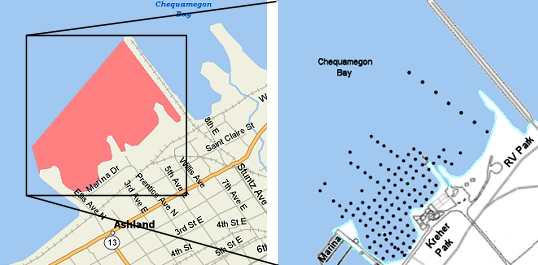
\includegraphics[width=6in]{Figs/Kreher_Park_Map.png}
  \caption{Location of the Ashland superfund site (left) with the location of 119 historical sediment sampling sites (right).}
  \label{fig:KreherParkMap}
\end{figure}

The WDNR wants to study elements in the sediment (among other things) in the entire area shaded in \figref{fig:KreherParkMap}.  This area covers approximately 3000 m$^2$.  Is it physically possible to examine every square meter of that area?  Is it prudent, ecologically and economically, to examine every square meter of this area?  The answer, of course, is ``no.''  How then will the WDNR be able to make conclusions about this entire area if they cannot reasonably examine the whole area?  The most reasonable solution is to sample a subset of all of this area and use the results from this sample to make inferences about the entire area.

Methods for properly selecting a sample that fairly represents a larger collection of individuals are an important area of study in the field of statistics.  For example, the WDNR would not want to sample areas that are only conveniently near shore because this will likely not be an accurate representation of the entire area to be studied.  In this example, it appears that the WDNR employed a grid to assure a relatively even dispersal of samples throughout the study area \figrefp{fig:KreherParkMap}.  Methods for choosing the number of individuals to select and how to select these individuals will be discussed in \chapref{chap:DataProd}.


Suppose that the WDNR measured the concentration of lead at each of the 119 locations shown in \figref{fig:KreherParkMap} and that they were to present the results from these data at a public meeting.  Further suppose that the WDNR scientist came to the meeting and showed a slide that simply had the list of lead concentration measurements on it \tabrefp{tab:KreherParkPbconc}\footnote{These are hypothetical data for this site.}.  Is it easy to come to any conclusion about what these data mean from this type of presentation?  Instead, suppose that the scientist came to the meeting with a simple plot of the frequency of concentrations present in the data and brief numerical summaries \figrefp{fig:KreherParkPbhist}.  With this presentation one can fairly easily see that the measurements were fairly symmetric with no obviously ``weird'' measurements and ranged from as low as 0.67 $\mu g \bullet m^{-3}$ to as high as 1.36 $\mu g \bullet m^{-3}$ with the measurements centered on approximately 1.0 $\mu g \bullet m^{-3}$.  These summaries will be discussed in detail in \chapref{chap:UnivEDA}.  However, at this point note that statistical methods are important for distilling or summarizing large quantities of data into graphs or numerical summaries from which it is much easier to identify characteristics of the data.

\begin{table}[htbp]   \label{tab:KreherParkPbconc}
  \caption{List of Pb concentration ($\mu g \bullet m^{-3}$) measurements at each of 119 sites in Kreher Park superfund site.}
  \begin{center}
\begin{knitrout}
\definecolor{shadecolor}{rgb}{1, 1, 1}\color{fgcolor}\begin{kframe}
\begin{verbatim}
  [1] 0.91 1.03 0.87 1.24 1.05 0.88 1.07 1.11 1.09 0.95 1.23 1.06 0.91 0.67 1.17 0.99
 [17] 1.00 1.14 1.12 1.09 1.14 1.12 1.01 0.70 1.09 0.99 0.98 0.78 0.93 1.06 1.20 0.98
 [33] 1.06 0.99 0.79 0.94 0.94 0.99 1.17 1.11 0.98 0.96 1.10 1.08 0.90 0.89 1.05 1.12
 [49] 0.98 1.13 1.06 0.91 1.05 0.83 1.21 1.30 0.94 0.84 1.09 0.98 1.36 0.99 1.10 1.00
 [65] 0.89 1.03 0.73 1.22 1.02 1.33 1.07 0.89 1.09 0.86 0.81 1.04 0.93 1.00 1.01 0.91
 [81] 0.91 0.98 1.18 0.77 1.09 1.05 1.16 0.95 1.06 1.04 0.92 1.18 1.17 1.11 1.24 1.08
 [97] 0.81 0.91 0.82 0.93 0.91 1.01 0.86 1.02 0.90 1.27 1.11 1.14 1.06 1.25 0.90 0.93
[113] 1.21 0.90 0.97 0.94 0.95 0.96 1.07
\end{verbatim}
\end{kframe}
\end{knitrout}
  \end{center}
\end{table}

\begin{knitrout}
\definecolor{shadecolor}{rgb}{0.922, 0.922, 0.922}\color{fgcolor}\begin{figure}[hbtp]

{\centering 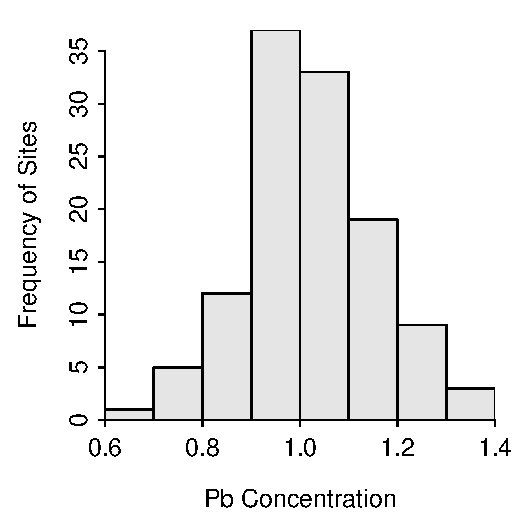
\includegraphics[width=.4\linewidth]{Figs/KreherParkPbhist-1} 
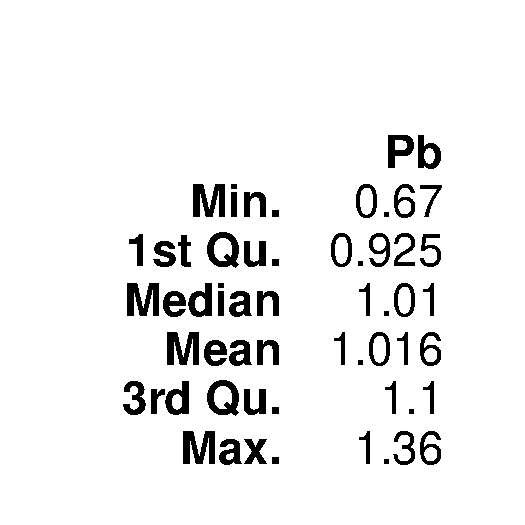
\includegraphics[width=.4\linewidth]{Figs/KreherParkPbhist-2} 

}

\caption[Histogram and summary statistics of Pb concentration ($\mu g \bullet m^{-3}$) measurements at each of 119 sites in Kreher Park superfund site]{Histogram and summary statistics of Pb concentration ($\mu g \bullet m^{-3}$) measurements at each of 119 sites in Kreher Park superfund site.}\label{fig:KreherParkPbhist}
\end{figure}


\end{knitrout}

A critical question at this point is whether or not the results from the one sample of 119 sites perfectly represents what the results would be for the entire area.  One way to consider this question is to examine the results obtained from another sample of 119 sites.  The results from this second sample \figrefp{fig:KreherParkPbhist1} are clearly, though not radically, different from the results of the first sample.  Thus, it is seen that any one sample from a large area will not perfectly represent the area.  Furthermore, it is observed that two different samples give two different results which will likely lead to two different, albeit generally only slightly different, conclusions.

\begin{knitrout}
\definecolor{shadecolor}{rgb}{0.922, 0.922, 0.922}\color{fgcolor}\begin{figure}[hbtp]

{\centering 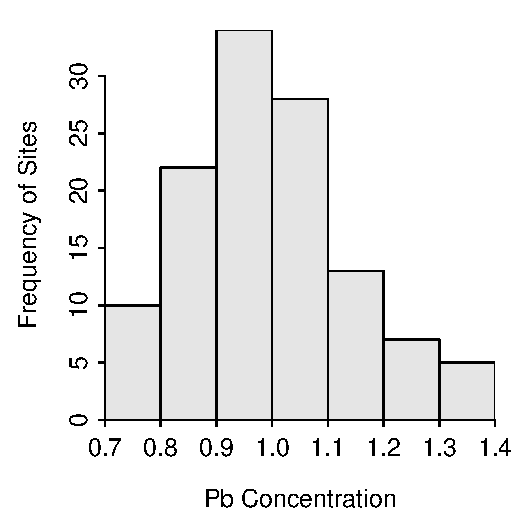
\includegraphics[width=.4\linewidth]{Figs/KreherParkPbhist1-1} 
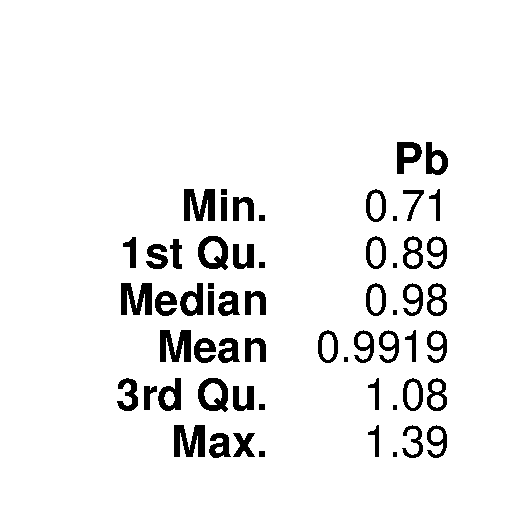
\includegraphics[width=.4\linewidth]{Figs/KreherParkPbhist1-2} 

}

\caption[Kreher Park 1]{Histogram and summary statistics of Pb concentration ($\mu g \bullet m^{-3}$) measurements at each of 119 sites (different from the sites shown in \figref{fig:KreherParkPbhist}) in Kreher Park superfund site.}\label{fig:KreherParkPbhist1}
\end{figure}


\end{knitrout}

The results of two different samples do not perfectly agree because each sample contains different individuals, and no two individuals are exactly alike in every regard.  The fact that no two individuals are exactly alike is \textbf{natural variability}\index{Natural Variability!Definition}, because of the ``natural'' differences that occur among individuals.  The fact that the results from different samples are different is called \textbf{sampling variability}\index{Sampling Variability!Definition}.  If there was no natural variability, then there would be no sampling variability.  If there was no sampling variability, then the field of statistics would not be needed because a sample (even of 1) would perfectly represent the larger group of individuals.  Thus, understanding variability is at the core of statistical practice.  These concepts of natural and sampling variability will be revisited continuously throughout this book.

\defn{Natural Variability}{The fact that no two individuals are exactly alike.}

\vspace{-12pt}
\defn{Sampling Variability}{The fact that the results (i.e., statistics) from different samples are different.}

This may all be a bit unsettling!  First, it was shown that an entire area or all of the individuals of interest cannot be examined.  It was then shown that a sample drawn to represent the population does not perfectly represent it.  Furthermore, each sample is unique and will likely lead to a different conclusion.  These are all real and difficult issues faced by the practicing scientist and considered by the informed consumer.  However, the field of statistics is designed to ``deal with'' these issues such that the results from a relatively small subset of measurements can be used to make conclusions about the entire collection of measurements.

\warn{Statistics provides methods for overcoming the difficulties caused by the requirement of sampling and the presence of sampling variability.}


\subsection{Purpose of Statistics}
The field of statistics has two primary purposes as illustrated in the Kreher Park example.  First, statistics provides methods to summarize large quantities of data into concise and informative numerical or graphical summaries.  For example, it is easier to discern the general underlying structure of the lead measurements from the statistics and histograms presented in \figref{fig:KreherParkPbhist} and \figref{fig:KreherParkPbhist1} than it is from the full list of lead measurements in \tabref{tab:KreherParkPbconc}.  Second, statistical methods allow inferences to be made about populations from samples.  These words will be defined more specifically in \sectref{sect:IVPPSS}, but this purpose is the process of making conclusions about the entire area or group of interest from a sample or subset of the individuals.

\warn{Statistics, as a field of study, is used to (1) summarize large quantities of data and (2) make inferences about populations from samples.}


\subsection{Definition of Statistics}
With the Kreher Park example in mind, let's consider a definition of statistics.  Statistics is the science of collecting, organizing, and interpreting numerical information or data \citep{MooreMcCabe1998}\index{Statistics, Field of!Definition}.  People (students and professionals) study statistics for a variety of reasons, including \citep{Bluman2000}:
\begin{Enumerate}
  \item They must be able to read and understand the statistical studies performed in their field. To have this understanding they must be knowledgeable about the vocabulary, symbols, concepts, and statistical procedures used in these studies.
  \item They may need to conduct research in their field. To accomplish this they must be able to design experiments and samples; collect, organize, analyze, and summarize data; and possibly make reliable predictions or forecasts for future use. They must also be able to communicate the results of the study.
  \item They also need to be better consumers of statistical information.
\end{Enumerate}

\defn{Statistics}{The science of collecting, organizing, and interpreting numerical information or data.}

The science of statistics permeates a wide variety of disciplines. \cite{MooreMcCabe1998} state:
\begin{quote}
The study and collection of data are important in the work of many professions, so that training in the science of statistics is valuable preparation for a variety of careers.  Each month, for example, government statistical offices release the latest numerical information on unemployment and inflation.  Economists and financial advisers, as well as policy makers in government and business study these data in order to make informed decisions.  Doctors must understand the origin and trustworthiness of the data that appear in medical journals if they are to offer their patients the most effective treatments. Politicians rely on data from polls of public opinion.  Business decisions are based on market research data that reveal customer tastes.  Farmers study data from field trials of new crop varieties.  Engineers gather data on the quality and reliability of manufactured products.  Most areas of academic study make use of numbers, and therefore also make use of the methods of statistics.
\end{quote}

\begin{exsection}


  \item \label{revex:WhyStatsLakes} There are 1499 lakes in Ashland, Bayfield, and Douglas counties of Wisconsin.  However, only 605 of these are named.  A random sample of named lakes from this population is extracted with the following R code:
\vspace{-12pt}
\begin{knitrout}
\definecolor{shadecolor}{rgb}{0.922, 0.922, 0.922}\color{fgcolor}\begin{kframe}
\begin{verbatim}
> library(NCStats)
> data(ABDLakes)
> named <- filterD(ABDLakes,named)
> srsdf(named,n=50,vars=c("county","area"))
\end{verbatim}
\end{kframe}
\end{knitrout}
Use this code and some hand (or calculator) calculations to answer the questions below. \ansref{ans:WhyStatsLakes}
    \begin{Enumerate}
      \item Extract a sample of 50 lakes with the code above.  Compare the size (area in acres) of the first two lakes.  What do you observe?  This is an example of what type of variability?
      \item Compute the proportion of lakes in your sample that are from Bayfield county.
      \item Extract another sample of 50 lakes.  Compare the proportion of lakes that are from Bayfield county in this sample to the proportion from your first sample.  What do you observe?  This is an example of what type of variability?
      \item Of the named lakes in the three counties, 346 are from Bayfield county.  Was the proportion of lakes from Bayfield County in either of your samples equal to the proportion of all named lakes that were from Bayfield County?  Were you surprised?  Why or why not?
    \end{Enumerate}
\end{exsection}


\section{IVPPSS}  \label{sect:IVPPSS}
\textbf{Statistical inference} is the process of forming conclusions about the unknown parameters of a population by computing statistics from the individuals in a sample.\index{Inference!Definition}  As you can imagine from this definition, it is important that you understand the difference between a population and a sample and a parameter and a statistic before you can understand and appreciate the process of making statistical inferences.  Before identifying these items you must also identify the individual and variable(s) of interest.  These six items must be explicitly identified at the beginning of any statistical analysis for that analysis to be conducted properly.  Understanding and identifying these items is the focus of this section.  Formal methods of inference will be discussed beginning with \chapref{chap:ProbIntro}.

\defn{Inference}{The process of forming conclusions about the unknown parameters of a population by computing statistics from the individuals in a sample.  As you can imagine from this definition, it is important that you understand the difference between a population and a sample.}

Throughout this section we will identify the individual, variable, population, parameter, sample, and statistic (referred to as the \textbf{IVPPSS}) for the following hypothetical example.  Assume that interest is in determining the average (or mean) length of the 1015 fish in Square Lake \figrefp{fig:SquareLakePopn}.  Note that in ``real life'' we would not know how many fish are in this lake.  However, for the purpose of illustrating the concepts of this chapter we will suppose that specific values of several variables for all 1015 fish in this lake are known.

\begin{knitrout}
\definecolor{shadecolor}{rgb}{0.922, 0.922, 0.922}\color{fgcolor}\begin{figure}[hbtp]

{\centering 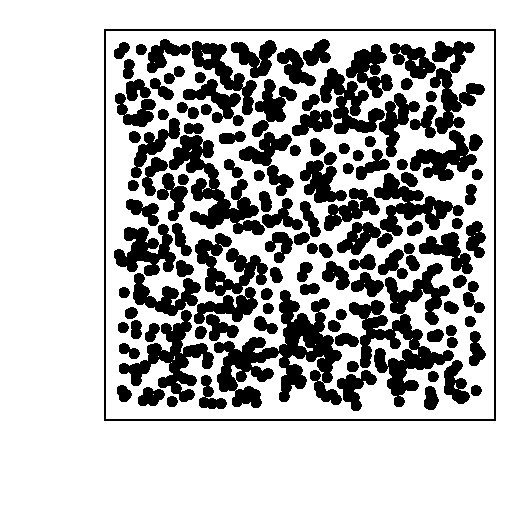
\includegraphics[width=.4\linewidth]{Figs/SquareLakePopn-1} 
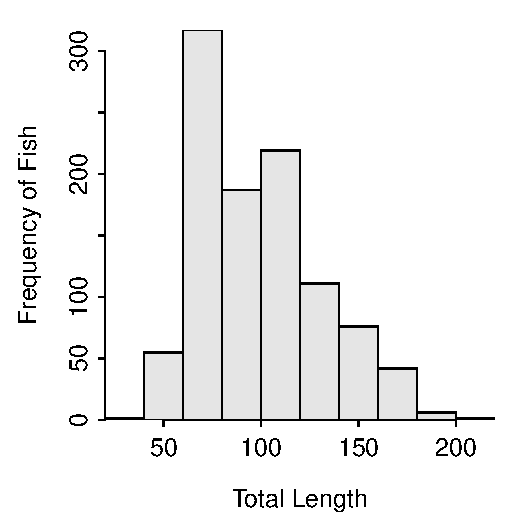
\includegraphics[width=.4\linewidth]{Figs/SquareLakePopn-2} 

}

\caption{Schematic representation (\textbf{Left}) of the 1015 fish (i.e., dots) in Square Lake and histogram (\textbf{Right}) of the total length of all 1015 fish in the Square Lake Population.}\label{fig:SquareLakePopn}
\end{figure}


\end{knitrout}

\subsection{Definitions}
The \textbf{individual} in a statistical analysis is one of the ``items'' that will be examined by the researcher.\index{Individual, Definition}  Sometimes the individual is a person, but it may be an animal, a piece of wood, a site or location, a particular time, or an event.  It is extremely important that you don't always visualize a person when you use the word individual in a statistical context.  Synonyms for individual are unit, experimental unit (usually used in experiments), sampling unit (usually used in observational studies), case, and subject (usually used in studies involving humans).  The individual of interest in the Square Lake example is an individual fish, because the researcher will collect a set of fish and examine each one individually.

\defn{Individual}{One of the items examined by the researcher.}

\vspace{-12pt}
\warn{An individual is not necessarily a person.}

The \textbf{variable} is the characteristic of interest about each individual.\index{Variable!Definition}  The variable is the information that the researcher records about each individual. The variable of interest in the Square Lake example is the length of each fish. Note that in most ``real life'' studies the researcher will be interested in more than one variable.  For example, in this example, the researcher may also record the fish's weight, sex, and age.  Studies with one variable are called univariate studies, studies with two variables are bivariate studies, and studies with more than two variables are called multivariate studies.

\defn{Variable}{The characteristic of interest about each individual.}

A \textbf{population} is the collection of ALL individuals of interest.\index{Population}  Simply put, the population is all of the individuals.  In the Square Lake example, the population is all 1015 fish in the lake.  You should define the population as thoroughly as possible including all qualifiers as necessary.  This example is simple because Square Lake is so well defined; however, as you will see in the chapter review exercises the population is often only well-defined by your choice of descriptors.

\defn{Population}{The collection of ALL individuals of interest.}

A \textbf{parameter} is a summary computed from ALL individuals in a population.\index{Parameter!Definition}  The term for the particular summary is usually preceded by the word ``population.''  Parameters are ultimately what is of interest because interest is in all individuals in the population.  However, in practice, parameters cannot be computed because the entire population cannot be ``seen.''  In this hypothetical example, all 1015 fish are accessible and the parameters are computed \tabrefp{tab:SquareLakePopn}\footnote{We will discuss how to compute and interpret each of these values in later chapters.}.  As stated above, in this example, interest is in the population mean (or average) length of all fish in Square Lake, which is 98.06 mm.

% latex table generated in R 3.3.1 by xtable 1.8-2 package
% Sat Aug 27 14:27:45 2016
\begin{table}[ht]
\centering
\caption{Summary parameters for the total length of all 1015 fish in the Square Lake population.} 
\label{tab:SquareLakePopn}
\begin{tabular}{cccccccccc}
 n & nvalid & mean & sd & min & Q1 & median & Q3 & max & percZero \\ 
  \hline
1015 & 1015 & 98.06 & 31.49 & 39 & 72 & 93 & 117 & 203 & 0.0 \\ 
   \hline
\end{tabular}
\end{table}


\defn{Parameter}{A summary of all individuals in a population.}

\vspace{-12pt}
\warn{Populations and parameters can generally not be ``seen.''}

The entire population cannot be ``seen'' in real life.  Thus, the only alternative for learning something about the population is to examine a subset of the population.  This subset is called a \textbf{sample}.\index{Sample!Definition}  The red dots in \figref{fig:SquareLakeSample1} represent a random sample of 50 fish from Square Lake (note that the sample size is usually denoted by a lower-case n; i.e., n=50).

\begin{knitrout}
\definecolor{shadecolor}{rgb}{0.922, 0.922, 0.922}\color{fgcolor}\begin{figure}[hbtp]

{\centering 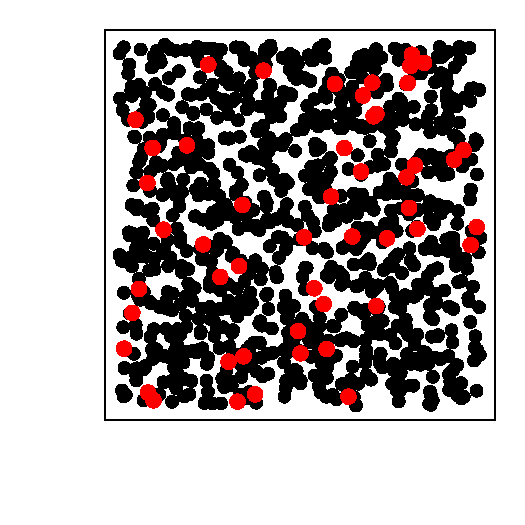
\includegraphics[width=.4\linewidth]{Figs/SquareLakeSample1-1} 
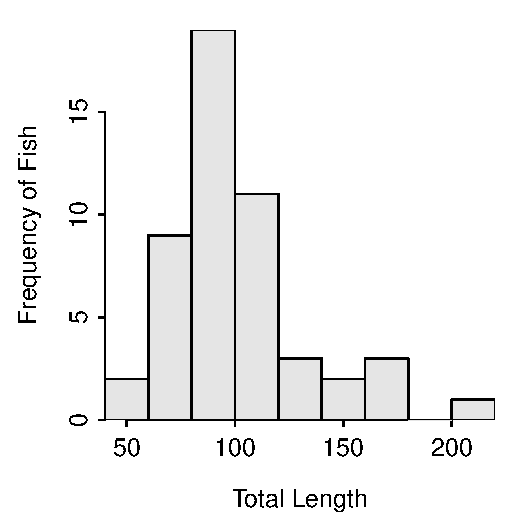
\includegraphics[width=.4\linewidth]{Figs/SquareLakeSample1-2} 

}

\caption{Schematic representation (\textbf{Left}) of a sample of 50 fish (i.e., red dots) from Square Lake and histogram (\textbf{Right}) of the total length of the 50 fish in this sample.}\label{fig:SquareLakeSample1}
\end{figure}


\end{knitrout}

\defn{Sample}{A subset of the population examined by a researcher.}

Summaries computed from individuals in a sample are called \textbf{statistics}.\index{Statistic!Definition}  Specific names of statistics should be preceded by the word ``sample.''  The statistic of interest is always the same as the parameter of interest; i.e., the statistic describes the sample the same way that the parameter describes the population.  For example, if interest is in the population mean, then the sample mean would be computed.  Some statistics computed from this sample are shown in \tabref{tab:SquareLakeSample1} and \figref{fig:SquareLakeSample1}.  The sample mean of 100.04 mm is the best ``guess'' at the population mean.  Not surprisingly from the discussion in \sectref{sect:WhyStats}, the sample mean does not perfectly equal the population mean.

% latex table generated in R 3.3.1 by xtable 1.8-2 package
% Sat Aug 27 14:27:45 2016
\begin{table}[ht]
\centering
\caption{Summary statistics for the total length of a sample of 50 fish from the Square Lake population.} 
\label{tab:SquareLakeSample1}
\begin{tabular}{cccccccccc}
 n & nvalid & mean & sd & min & Q1 & median & Q3 & max & percZero \\ 
  \hline
50 & 50 & 100.04 & 31.94 & 49 & 81 & 91 & 118 & 203 & 0.0 \\ 
   \hline
\end{tabular}
\end{table}



\subsection{Performing an IVPPSS}
In each statistical analysis it is important that you determine the Individuals, Variable, Population, Parameter, Sample, and Statistics (IVPPSS).  It is simplest to do this in this order -- IVPPSS.  First, determine what items you are actually going to look at; those are your individuals.  Second, what are you going to record when you look at an individual; that is the variable.  Third, the population is simply ALL of the individuals.  Fourth, the parameter is a summary (e.g., mean or proportion) of the variable recorded from all of the individuals in the population\footnote{Again, parameters generally cannot be computed because all of the individuals in the population can generally not be seen.  Thus, the parameter is largely conceptual.}.  Fifth, we realize that we cannot see all of the individuals in the population so we examined only a few -- those few were the sample.  Finally, the summary of the individuals in the sample is the statistic.  The statistic has to be the same summary of the sample as the parameter was of the population.

When performing an IVPPSS, keep in mind that parameters describe populations (note that they both start with ``p'') and statistics describe samples (note that they both start with ``s'').  This can also be looked at from another perspective.  A sample is an estimate of the population and a statistic is an estimate of a parameter.

This process can be illustrated by performing an IVPPSS for the following situation:
\begin{quote}
\textit{A University of New Hampshire graduate student (and Northland College alum) investigated habitat utilization by New England (Sylvilagus transitionalis) and Eastern (Sylvilagus floridanus) cottontail rabbits in Maine.  In a preliminary portion of his research he wants to determine the proportion of ``rabbit patches'' that are inhabited by New England cottontails.  In the winter of 1999 he examined 70 ``patches'' and found that 53 showed evidence of inhabitance by New England cottontails.}
\end{quote}

\begin{Itemize}
  \item The individuals are the rabbit patches (i.e., a rabbit patch is the ``item'' being sampled and examined).
  \item The variable is ``evidence for New England cottontails or not (yes or no)'' (i.e., the characteristic of each rabbit patch that was recorded).
  \item The population is ALL rabbit patches in Maine.
  \item The parameter is the proportion of ALL rabbit patches in Maine that showed evidence for New England cottontails\footnote{Note that this population and parameter cannot actually be calculated but it is what the researcher wants to know.}.
  \item The sample is the 70 rabbit patches in Maine that were actually examined by the researcher.
  \item The statistic is the proportion of the 70 rabbit patches in Maine actually examined that showed evidence for New England cottontails\footnote{Note that this statistic is the same as the parameter; it is just computed on a different collection of individuals.}.
\end{Itemize}

In some situations it may be easier to start by identifying the sample.  From this, and through the realization that a sample is always ``of the individuals'', it may be easier to identify the individual.  This process is illustrated in the following example, with the items listed in the order identified rather than in the traditional IVPPSS order.

\begin{quote}
\textit{The Duluth, MN touristry board is interested in the average number of raptors seen per year at Hawk Ridge\footnote{Information about Hawk Ridge is found \href{http://www.hawkridge.org/}{here}.}.  To determine this value they collected the total number of raptors seen in a sample of years from 1971-2003.}
\end{quote}

\begin{Itemize}
  \item The sample is the 32 years between 1971-2003 at Hawk Ridge.
  \item An individual is a year (because a ``sample of \emph{years}'' was taken) at Hawk Ridge.
  \item The variable recorded was the number of raptors seen in one year.
  \item The population is ALL years (this is a bit ambiguous but may be thought of as all years that Hawk Ridge has existed).
  \item The parameter is the average number of raptors seen per year in ALL years.
  \item The statistic is the average number of raptors seen in the 1971-2003 sample of years.
\end{Itemize}


\begin{exsection}
  \item \label{revex:IVPPSSDad}My Dad owns 60 acres of timber (mostly Oak, Walnut, and Poplar) in Iowa.  He wants to measure the mean diameter-at-breast-height (DBH) of the oak trees on his property.  He measures the DBH of 75 randomly selected oak trees.  Use this information to perform an IVPPSS. \ansref{ans:IVPPSSDad}
  \item \label{revex:IVPPSSFishStore}I have a friend who wants to start a (fishing) bait store on the West end of Ashland.  He wants to determine what proportion of Ashland residents who currently use the East end bait store would use a store in the West end if one existed.  He sends out 5000 questionnaires and receives 2378 back from patrons of the East end store.   Use this information to perform an IVPPSS.  \ansref{ans:IVPPSSFishStore}
  \item \label{revex:IVPPSSNBA}I'm interested in developing a model to predict how many points an NBA starting basketball player scores. Therefore, I want to determine the relationship between points scored and height, speed (in the 40-yard dash), position, and minutes played. To identify this relationship I gather these data from 100 NBA starting basketball players.  Use this information to perform an IVPPSS. \ansref{ans:IVPPSSNBA}
  \item \label{revex:IVPPSSClinton}Pollsters wanted to determine the proportion of registered voters who approved of President Clinton's performance.  They called 5000 randomly selected registered voters and ask 4123 of those (the rest weren't home, didn't answer, or hung up) ``Do you approve of Pres. Clinton's performance?''  Use this information to perform an IVPPSS. \ansref{ans:IVPPSSClinton}
  \item \label{revex:IVPPSSGoslings}You Might Be Interested To Know (YMBITK), the average level of mercury in newly-hatched goslings in the upper Midwest (MI, MN, ND, SD, WI). You obtained 20 goslings from resource agencies in each state.  Use this information to perform an IVPPSS. \ansref{ans:IVPPSSGoslings}
  \item \label{revex:IVPPSSNClead}YMBITK, the proportion of NC students that think NC can become ``the nation's leading environmental liberal arts college'' in the next decade. You polled 124 students.  Use this information to perform an IVPPSS. \ansref{ans:IVPPSSNClead}
  \item \label{revex:IVPPSSStudy}YMBITK, the relationship between hours studied and GPA of students in the UW system (excluding UW-Madison). You interviewed 250 students from throughout the system.  Use this information to perform an IVPPSS. \ansref{ans:IVPPSSStudy}
  \item \label{revex:IVPPSSCoach}YMBITK, the average difference in salaries between the head coaches of men's and head coaches of women's basketball teams at Division I schools. You interviewed 73 head-coach pairs.  Use this information to perform an IVPPSS. \ansref{ans:IVPPSSCoach}
  \item \label{revex:IVPPSSBioGrads}YMBITK, the proportion of graduates from small private schools, who majored in Biology and who have been out of school for at least 5 years, that feel that statistics is an ``important'' course. You interviewed 1023 people.  Use this information to perform an IVPPSS. \ansref{ans:IVPPSSBioGrads}
  \item \label{revex:IVPPSSBaikal}Scientist in Chivyrkui Bay on Lake Baikal \citep{OwensPronin2000} were interested, among other things, in determining the mean age of pike (\textit{Esox lucius}) in the bay. They collected scales from 30 fish using gill nets and angling methods. Use this information to perform an IVPPSS. \ansref{ans:IVPPSSBaikal}
  \item \label{revex:IVPPSSRuffe}The Eurasian ruffe is an exotic species of fish that is causing some alarm in fisheries biologists in the Great Lakes area \citep{Maniaketal2000}. A few of these biologists tested to see if a certain pheromone released by injured ruffe would repel other ruffe.  If so, natural, or possibly synthetic, versions of this pheromone could be used to distract ruffe from areas in which they are causing damage. In their experiment, they observed ruffe held in aquaria divided into four sections.  They recorded what proportion of 24 randomly-selected ruffe caught in the St. Louis River Harbor, and then held in the aquaria, left a section when the chemical was added to that section.  Use this information to perform an IVPPSS. \ansref{ans:IVPPSSRuffe}
\end{exsection}


\subsection{Sampling Variability, Again}
It is instructive to once again consider how the statistics might change when different samples are taken.  \tabref{tab:SquareLakeSample234} and \figref{fig:SquareLakeSample234} show the results from three more samples of 50 fish from the Square Lake population.  All four samples (including the sample shown in \tabref{tab:SquareLakeSample1} and \figref{fig:SquareLakeSample1}) had means that were quite different from the known population mean of 98.06.  All four histograms were similar in appearance but were slightly different in actual values.  Similar conclusions could be made for the other parameters and statistics (e.g., compare the population and sample standard deviations, min, max, etc.).  The concept illustrated here is that a sample will likely represent the population of interest, but there will be variability among samples.  This variability between samples is called \textbf{sampling variability}, which is one of the most important concepts in statistics and will be discussed in great detail throughout this class.\index{Sampling Variability!Definition}

\begin{knitrout}
\definecolor{shadecolor}{rgb}{0.922, 0.922, 0.922}\color{fgcolor}\begin{figure}[hbtp]

{\centering 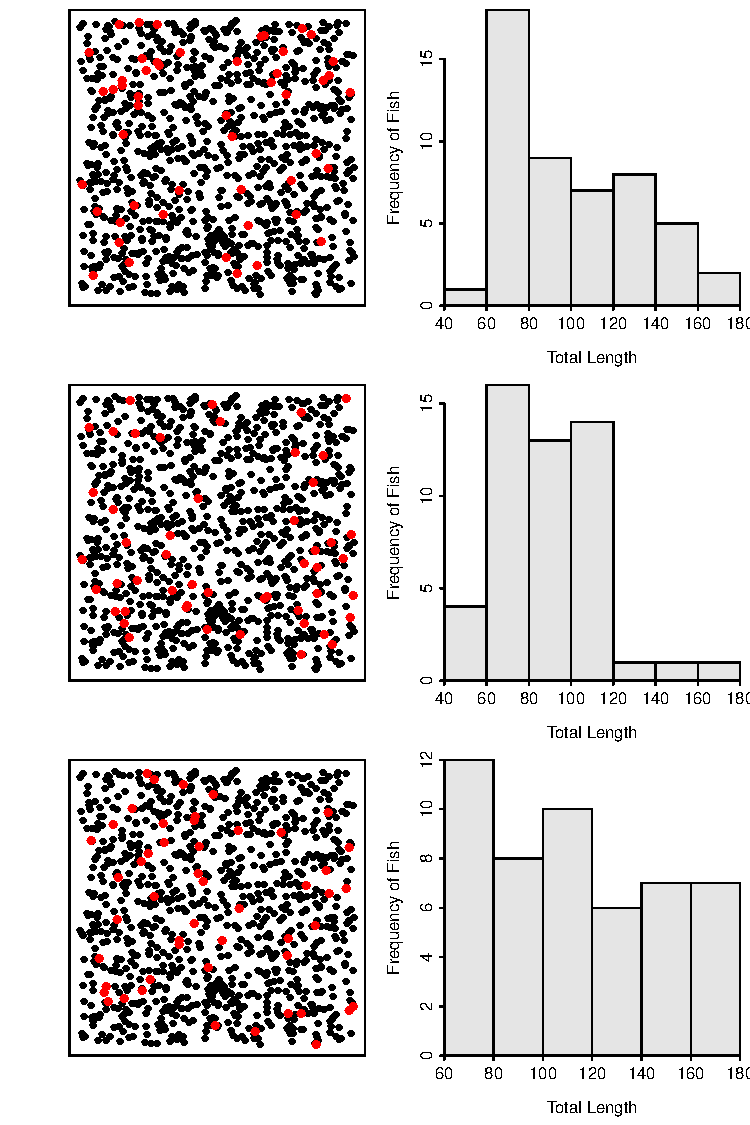
\includegraphics[width=.7\linewidth]{Figs/SquareLakeSample234-1} 

}

\caption{Schematic representation (\textbf{Left}) of three samples of 50 fish (i.e., red dots) from Square Lake and histograms (\textbf{Right}) of the total length of the 50 fish in each sample.}\label{fig:SquareLakeSample234}
\end{figure}


\end{knitrout}

% latex table generated in R 3.3.1 by xtable 1.8-2 package
% Sat Aug 27 14:27:45 2016
\begin{table}[htbp]
\centering
\caption{Summary statistics for the total length in three samples of 50 fish from the Square Lake population.} 
\label{tab:SquareLakeSample234}
\begin{tabular}{cccccccccc}
 n & nvalid & mean & sd & min & Q1 & median & Q3 & max & percZero \\ 
  \hline
50 & 50 & 99.56 & 32.47 & 57 & 69 & 91 & 123 & 167 & 0.0 \\ 
  50 & 50 & 88.64 & 24.52 & 53 & 68 & 86 & 106 & 166 & 0.0 \\ 
  50 & 50 & 112.74 & 35.86 & 61 & 84 & 108 & 147 & 174 & 0.0 \\ 
   \hline
\end{tabular}
\end{table}


\defn{Sampling Variability}{The realization that no two samples are exactly alike. Thus, statistics computed from different samples will likely vary.}

This example also illustrates another important statistical concept.  Parameters are fixed values because populations don't change.  If a population does change, then it is considered to be a different population.  In the Square Lake example, if a fish is removed from the lake, then the lake would then be considered a different population of fish.  Statistics, on the other hand, vary in value depending on the sample because each sample consists of different individuals and individuals vary (i.e., sampling variability exists because natural variability exists).

\warn{Parameters are fixed in value, while statistics vary in value.}


\section{Variable Types}\label{sect:VarTypes}
The type of statistic that can be calculated is dictated by the type of variable to be analyzed.  For example, a sample mean (or average) can only be calculated for a quantitative variable (defined below).  Thus, immediately after identifying the variable in the IVPPSS procedure you should identify the type of that variable.


\subsection{Variable Definitions}
There are two main groups of variable types -- quantitative and categorical \figrefp{fig:VarTypes}.  \textbf{Quantitative} variables are variables with numerical values for which it makes sense to do arithmetic operations (like adding or averaging).\index{Quantitative Variable}  Synonyms for quantitative are measurement or numerical.  \textbf{Categorical} variables are variables that record to which group or category an individual belongs.\index{Categorical Variable}  Synonyms for categorical are qualitative or attribute.  Within each main type of variable are two subgroups \figrefp{fig:VarTypes}.

\begin{knitrout}
\definecolor{shadecolor}{rgb}{0.922, 0.922, 0.922}\color{fgcolor}\begin{figure}[hbtp]

{\centering 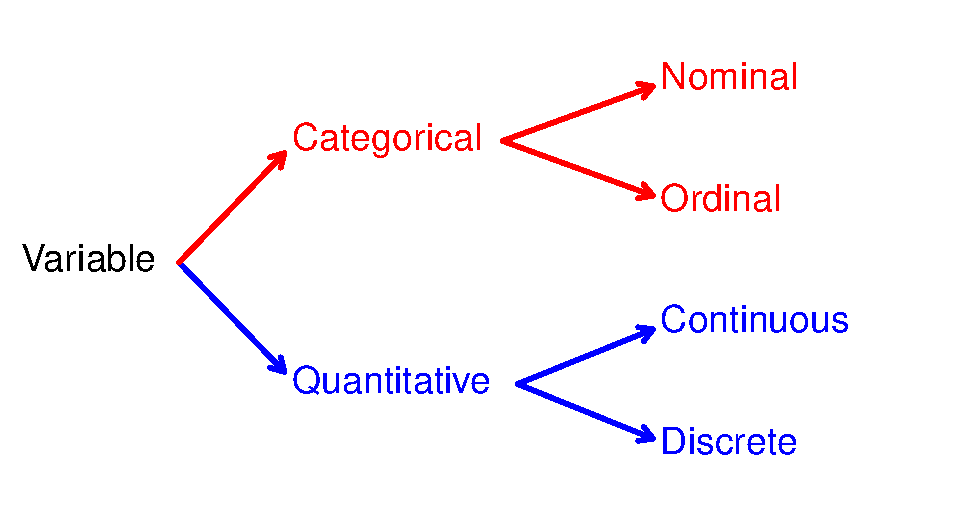
\includegraphics[width=.7\linewidth]{Figs/VarTypes-1} 

}

\caption[Schematic representation of the four types of variables]{Schematic representation of the four types of variables.}\label{fig:VarTypes}
\end{figure}


\end{knitrout}
\vspace{9pt} % added because of paragraph compressions following R code

The two types of quantitative variables are continuous and discrete variables.  \textbf{Continuous} variables are quantitative variables that have an uncountable number of values.\index{Continuous Variable}  In other words, a potential value \textsc{does} exist between every pair of values of a continuous variable.  \textbf{Discrete} variables are quantitative variables that have a countable number of values.\index{Discrete Variable}  Stated differently, a potential value \textsc{does not} exist between every pair of values of a discrete variable.  Typically, but not always, discrete variables are counts of items.

Continuous and discrete variables are easily distinguished by determining if it is possible for a value to exist between every two values of the variable.  For example, can there be between 2 and 3 ducks on a pond?  No!  Thus, the number of ducks is a discrete variable.  Alternatively, can a duck weigh between 2 and 3 kg?  Yes!  Can it weigh between 2 and 2.1 kg?  Yes!  Can it weigh between 2 and 2.01 kg?  Yes!  You can see that this could continue forever.  Thus, duck weight is a continuous variable.

\defn{Discrete Variable}{A quantitative variable that can assume a countable number of values.}

\vspace{-12pt}
\defn{Continuous Variable}{A quantitative variable that can assume an uncountable number of values.}

\vspace{-12pt}
\warn{A quantitative variable is continuous if a possible value exists between every two values of the variable; otherwise, it is discrete.}

The two types of categorical variables are ordinal and nominal.  \textbf{Ordinal} variables are categorical variables where a natural order or ranking exists among the categories.\index{Ordinal Variable}  \textbf{Nominal} variables are categorical variables where no order or ranking exists among the categories.\index{Nominal Variable}

Ordinal and nominal variables are easily distinguished by determining if the order of the categories matters.  For example, suppose that a researcher recorded a subjective measure of condition (i.e., poor, average, excellent) and the species of each duck.  Order matters with the condition variable -- i.e., condition improves from the first (poor) to the last category (excellent) -- and some reorderings of the categories would not make sense -- i.e., average, poor, excellent does not make sense.  Thus, condition is an ordinal variable.  In contrast, species (e.g., mallard, redhead, canvasback, and wood duck) is a nominal variable because there is no inherent order among the categories (i.e., any reordering of the categories also ``makes sense'').

\defn{Ordinal Variable}{A categorical variable for which a natural order exists among the categories.}

\vspace{-12pt}
\defn{Nominal Variable}{A categorical variable for which a natural order DOES NOT exist among the categories.}

\vspace{-12pt}
\warn{Remember that \textbf{ord}inal means that an \textbf{ord}er among the categories exists (note ``ord'' in both ordinal and order).}

The following are some issues to consider when identifying the type of a variable:
\begin{Enumerate}
  \item The categories of a categorical variable are sometimes labeled with numbers.  Don't let this fool you into calling the variable quantitative.
  \item Rankings, ratings, and preferences are ordinal (categorical) variables.
  \item Counts of numbers are discrete (quantitative) variables.
  \item Measurements are typically continuous (quantitative) variables.
  \item Categorical variables that consist of only two levels or categories will be labeled as a nominal variable (because any order of the groups makes sense).  This type of variable is also often called a ``binomial'' variable.
  \item Do not confuse ``what type of variable'' (answer is one of ``continuous'', ``discrete'', ``nominal'', or ``ordinal'')  with ``what type of variability'' (answer is ``natural'' or ``sampling'') questions.
\end{Enumerate}

\warn{``What type of variable is ...?'' is a different question than ``what type of variability is ...?''  Be careful to note the word difference (i.e., ``variable'' versus ``variabiltiy'' when answering these questions.}

\begin{exsection}
  \item \label{revex:VarTypeDucks} What type of variable is the number of ducks found at the ``Hot Pond'' every morning? \ansref{ans:VarTypeDucks}
  \item \label{revex:VarTypeGenetics} What type of variable is the genotype (AA, Aa, aa) of a particular species of sunflower? \ansref{ans:VarTypeGenetics}
  \item \label{revex:VarTypeGenetics2} What type of variable is the length of petals on individual flowers? \ansref{ans:VarTypeGenetics2}
  \item \label{revex:VarTypeGenetics3} What type of variable is the number of seeds produced by an individual sunflower? \ansref{ans:VarTypeGenetics3}
  \item \label{revex:VarTypeGenetics4} What type of variable is the ``quality'' of the seeds produced by an individual plant (``quality'' is recorded as 1=poor, 2=low, 3=good, and 4=excellent)? \ansref{ans:VarTypeGenetics4}
  \item \label{revex:VarTypeSOS} What type of variable is student rankings (``Excellent'', ``Very Good'', ``Good'', ``Fair'', ``Poor'') of a professor's abilities? \ansref{ans:VarTypeSOS}
  \item \label{revex:VarTypeAudit} What type of variable is whether an account is valid or invalid? \ansref{ans:VarTypeAudit}
  \item \label{revex:VarTypeDefects} What type of variable is the number of defects produced by a machine? \ansref{ans:VarTypeDefects}
  \item \label{revex:VarTypeBottles} What type of variable is the ounces of cola in a sample of 100 bottles? \ansref{ans:VarTypeBottles}
  \item \label{revex:VarTypeFish} What type of variable is the sex of fish collected from a lake? \ansref{ans:VarTypeFish}
  \item \label{revex:VarTypeFrogs} What type of variable is the number of legs on frogs collected in Bayfield County? \ansref{ans:VarTypeFrogs}
  \item \label{revex:VarTypeCroak} What type of variable is the frequency (mhz) of a bullfrog's ``croak''? \ansref{ans:VarTypeCroak}
  \item \label{revex:VarTypeTowns} What type of variable is the number of incorporated towns in a county? \ansref{ans:VarTypeTowns}
  \item \label{revex:VarTypeWeasels} What type of variable is the qualitative size of least weasels (small, medium, large)? \ansref{ans:VarTypeWeasels}
\end{exsection}


\newpage
\section{Writing Homework Reports} \label{sect:ReportWriting}
I have very specific expectations for your homework assignment reports.  These expectations and requirements are described below.

\begin{Itemize}
  \item Each document should be labeled with your name and homework title (e.g., ``Chapter 10 Homework'').  It is not that important to me that you include the name of the class or my name (I already know both of these).
  \item Each document should include the following statement along with your signature -- ``\emph{I have neither given nor received unauthorized aid in completing this work, nor have I presented someone else's work as my own.}''
  \item Each document should be typed and printed to hand in as a hard-copy.
  \item Your document should ``look nice.''  This means that you should include spaces that increase readability (e.g., between a paragraph and a table) but remove spaces that waste paper (e.g., there is no need to have five empty lines between a paragraph and a graphic).  In addition, you should not use ``non-standard'' fonts -- the most common of which is ``comic sans.''  Scientific presentations require a ``serious'' font which is likely one of ``Times New Roman'', ``Arial'', ``Calibri'', or ``Helvetica''.  The one exception to this is the use of ``\texttt{Courier}'' for tabular results (see below).
  \item You should use complete sentences whenever possible.  This may result in very simple sentences -- e.g., ``The sample mean is 3.26 (Table 1).'' -- but should become your default.
  \item Generally, the document should be single-spaced (see \sectref{sect:RFAQSingleSpace} for making MSWord ``single space'' your document).
  \item You should provide evidence for each factual statement that you make.  Most of the time this means that you will be referring to a particular figure or table.  It is inappropriate to say ``in the table below'', for example.  Instead you should say ``as seen in Table 1'' or put ``(Table 1)'' at the end of a sentence.  Tables and figures should then be properly labeled (see below).
  \item Tables and figures should be properly labeled.  There are a wide variety of proper styles for labeling figures and tables.  The most common styles label tables ON TOP of the table and figures BELOW the figure.  The labels should include the words ``Table'' or ``Figure'' (note that ``Graph'' and ``Chart'' are unacceptable), should include a sequential number (the first of each table or figure is numbered ``1'' and each subsequent table or figure has an increased number), and a descriptive label.  Descriptive labels are \textbf{descriptive} -- i.e., ``Table 1.  Summary statistics of data.'' is inadequate, ``Table 1.  Summary statistics of the length of ant antennae separated by sex.'' is much better.  Examples of labeling standards are shown in \sectref{sect:RFAQLabels}.
  \item R output (usually as a table) should be converted to ``Courier'' or ``Courier (New)'' font.  This is the font used by R and, thus, will force the items in the table to ``line up.'' This will save you from having to include spaces or tabs to make items line up.  See \sectref{sect:RFAQCourier} on how to change the font.  ONLY R output should be in the ``Courier'' font.  All other text should be in the fonts mentioned previously.
  \item Where appropriate, Greek letters should be changed to their symbol equivalent.  In other words, it is better to use $\alpha$ than ``alpha.''  See \sectref{sect:RFAQGreek} for how to include these symbols in your analysis.
  \item Every assignment that uses R should include an appendix that lists the script of R commands used to produce the analyses (i.e., the code from your RStudio script window).  This script should contain only ``good'' commands and should not include any commands that produce errors or were not used in your analysis.
\end{Itemize}


\newpage
\begin{hwsection}{All questions below should be typed and answered following the expectations identified in \sectref{sect:ReportWriting}.  All work must be shown.  Questions marked with the R logo must include R output with your R commands in an attached appendix.}
  \item \label{hwprob:WhyStatsFrogs} Sigurd Olson Environmental Institute (SOEI) biologists were interested in estimating the total number of frogs on all lakes in northern Wisconsin (defined as north of Highway 8) in 2010.  They identified a sample of lakes in northern Wisconsin, and on each lake they used two methods to determine the number of frogs on the lake.  First, they counted the number of frogs seen as they walked the shoreline of the lake (called the \var{visual} count).  Second, they counted individual mating calls heard (called the \var{call} count).  Use this information to answer the questions below.
    \begin{Enumerate}
      \item What is an individual in this scenario?
      \item What type of variable is the number of frogs on a lake?
      \item Do you think it is reasonable to count the number of frogs on every lake in northern Wisconsin at the same time (say, in the same week)?  Why or why not?
      \item \rhw{} Extract a sample of 10 lakes using the \R{srsdf()} function and the \R{data(Frogs)} data frame in the \R{NCStats} package. [HINT: You can use these three lines of R code below.]  Copy the numbers for your sample and paste them in your report document.
\begin{knitrout}
\definecolor{shadecolor}{rgb}{0.922, 0.922, 0.922}\color{fgcolor}\begin{kframe}
\begin{verbatim}
> library(NCStats)
> data(Frogs)
> ( smpl1 <- srsdf(Frogs,n=10) )
\end{verbatim}
\end{kframe}
\end{knitrout}
\vspace{9pt}
      \item Compare the visual number of frogs recorded on the first two lakes.  What do you observe?  This is an example of what type of variability?
      \item Compute the average visual number of frogs in all lakes in your sample.  Show your work (you may leave space in your document and hand write your work before handing it in)!
      \item \rhw{} Extract another sample of 10 lakes.  Again, copy and paste the data into your document.
      \item Compare the average visual number of frogs in this sample (Show your work!) to the average from the first sample.  What do you observe?  This is an example of what type of variability?
      \item I happen to know that the average visual number of frogs on all lakes in northern Wisconsin (the population) is 225.  Was the average visual counts from both of your samples equal to this population value?  Were you surprised?  Why or why not?
    \end{Enumerate}

  \item \label{hwprob:WhyStatsVAR}Define natural and sampling variability.  Construct the narrative background for an example ``real-life'' situation and illustrate natural and sampling variability within the context of this example.

  \item \label{hwprob:WhyStatsReality}Identify and describe two ``realities'' that, if they did not exist, would eliminate the need for the field of statistics.

  \item \label{hwprob:IVPPSSCrayfish}A NC student, for their Biology capstone, wants to determine the mean carapace length of Rusty Crayfish (\textit{Orconectes rusticus}) in a lake with Smallmouth Bass (\textit{Micropterus dolomieu}). In 2012, the student gathered and examined 235 crayfish in a manner that was as random as possible.
    \begin{Enumerate}
      \item Use this information to identify the individual, variable, population, parameter, sample, and statistic.
      \item What type of variable is the carapace length of crayfish?
    \end{Enumerate}

\turnpage{24}

  \item \label{hwprob:IVPPSSWater} Many exotic aquatic organisms have been transferred to the Great Lakes in the ballast water of trans-oceanic ships.  To attempt to halt this invasion ships are required to release their ballast water before entering the St. Lawrence seaway.  Ships with cargo theoretically do not contain ballast.  However, their ballast tanks contain some residual amount of water and, thus, may harbor exotic organisms.  Researchers with Michigan Sea Grant (more information on page 9 \href{http://www.miseagrant.umich.edu/downloads/upwellings/sum02.pdf}{here}) examined the water found in 43 ballast tanks from 22 cargo-laden boats entering the Seaway in 2001.  They were interested in determining the proportion of ballast tanks that contained living organisms.
    \begin{Enumerate}
      \item Use this information to identify the individual, variable, population, parameter, sample, and statistic.
      \item What type of variable is the variable you identified?
    \end{Enumerate}

  \item \label{hwprob:VarTypeLead} In the beginning of this chapter, the concentration ($\mu g \bullet m^{-3}$) of lead at 119 sites in Chequamegon Bay was discussed.  What type of variable is the concentration of lead?

  \item \label{hwprob:VarTypeRisk} An actuary rates potential insurees as ``low risk'', ``moderate risk'', or ``high risk''.  What type of variable is this risk rating?

  \item \label{hwprob:VarTypeInfoType} A sociologist asked respondents from which medium they receive most of their information about wolves: ``TV'', ``Newspaper'', ``Outdoor Magazines'', ``Public Policy Meetings'', ``Friends or Family'', or ``Other''.  What type of variable is information type?

  \item \label{hwprob:VarTypeKoppen} The Koppen scheme of classifying ``climates'' contains five principal groups: ``tropical rainy'', ``dry'', ``temperate rainy'', ``cold snowy forest'', and ``polar''.  What type of variable is the Koppen scheme of classification?  Write a short sentence defending your choice.
\end{hwsection}



\chapter{Getting Started with R} \label{chap:FoundationsR}
\begin{ChapObj}{\boxwidth}
  \textbf{Chapter Objectives:}
  \begin{Enumerate}
    \item Understand the difference between R expressions and assignments.
    \item Understand the different types of data that can be stored in R.
    \item Understand the different types of data structures used in R.
    \item Be able to enter data into R data frames.
    \item Be able to isolate individual variables and individuals in R.
    \item Be able to create data frames that are subsets of larger data frames.
    \item Understand how homework assignments should be formatted.
  \end{Enumerate}
\end{ChapObj}

\minitoc
\newpage

\section{Setting Up R and Helpers} \label{sect:RSetup}
\vspace{-8pt}
Detailed methods for downloading, installing, and configuring R, RStudio, and \R{NCStats} on your personal computer are given on the \href{http://derekogle.com/NCMTH107/resources/}{Resources page of the course website}.

\vspace{-8pt}
\section{Working With R Basics} \label{sect:RBasics}
\vspace{-12pt}
\subsection{Saving Results} \label{sect:RSaving}
Results are not saved in R or RStudio.  Rather, ``scripts'' of successful R commands are saved and, then, if the analysis needs to be re-done, the entire set of commands is opened in RStudio and run again.  When writing a report, all tabular and graphical output should be copied from RStudio and pasted into your report document.  This document will serve as your analysis report and can be modified to include answers to questions, references to the tables and graphs, etc.  Specifics for how this report should be prepared are discussed in \sectref{sect:ReportWriting}.  All data that is not a simple vector (see \sectref{sect:RInfoStorage}) should be entered into R through text files (see \sectref{sect:REnterData}).  With this method, the data will only need to be typed once.

R does allow one to save a ``workspace.''  I strongly urge you to follow the three suggestions of the previous paragraph rather than saving the workspace.  Saving the workspace ``brings back'' objects that a student has either forgotten about, contain incorrect information, or otherwise clutter the work area.  Saving a workspace appears to cause trouble for most students.  Save your ``good'' commands in a script and save your ``good'' results in a report document; do not save the workspace.

\vspace{-8pt}
\subsection{Expressions and Assignments} \label{sect:RExprAssn}
\vspace{-8pt}
Expressions in R are mathematical ``equations'' that are evaluated by R with a result seen immediately.  An example of an expression in R is
\begin{knitrout}
\definecolor{shadecolor}{rgb}{0.922, 0.922, 0.922}\color{fgcolor}\begin{kframe}
\begin{verbatim}
> 5+log(7)-pi
[1] 3.804317
\end{verbatim}
\end{kframe}
\end{knitrout}

where \R{log()} and \R{pi} are built-in functions used to compute the natural log and find the value of $\pi$, respectively.  Expressions in R are like using a calculator where the result is shown on the console but it is not saved for any subsequent analyses.  In addition, expressions in R follow the same general rules as expressions entered into your calculator -- i.e., same order of operations and use of parentheses.

\warn{The results of expressions in R are temporary unless the result is assigned to an object.}

Typically you will want to save a computation for further computations.  This ``saving'' is accomplished by assigning the results of an expression to an object in R.  The results of an expression is assigned to an object with the assignment operator (i.e., \R{<-}).  The general form for saving the result of an expression into an object is \R{object <- expression}.  The result of the expression will not be seen unless the object name is subsequently typed into R (but see below).  For example, the result of the previous expression is saved into an object called \var{x} and then viewed with
\begin{knitrout}
\definecolor{shadecolor}{rgb}{0.922, 0.922, 0.922}\color{fgcolor}\begin{kframe}
\begin{verbatim}
> x <- 5+log(7)-pi
> x
[1] 3.804317
\end{verbatim}
\end{kframe}
\end{knitrout}
Many times one wants to also see the result of an expression immediately after it has been saved to an object.  As shown above, one can simply type the name of the object.  However, a short-cut for both assigning and printing the result of an expression is to surround the entire command in parentheses.  For example, the following both assigns the result of the expression to \var{y} and prints the result\footnote{Note that the spaces after the opening parentheses and before the closing parentheses are not needed.  However, they make the code more legible.},
\begin{knitrout}
\definecolor{shadecolor}{rgb}{0.922, 0.922, 0.922}\color{fgcolor}\begin{kframe}
\begin{verbatim}
> ( y <- 15*exp(2) )
[1] 110.8358
> # note that the next line is now not needed
> y
[1] 110.8358
\end{verbatim}
\end{kframe}
\end{knitrout}

\warn{The convention of surrounding commands in parentheses to both assign and print the results will be used extensively in this book to save space.}

As a general rule, you should assign your computations to an object so that the result can be easily retrieved later\footnote{Note, however, that each assignment uses computer memory.  Thus, if you know for sure that you will not need the result for later use, then do not assign it to an object.  Memory can also be made available by removing objects that are known to no longer be of use.  Objects are removed from R with \R{rm(objectname)}.  A list of current objects is obtained with \R{ls()} and all objects are removed with the \R{Menu..Remove All Objects} menu item.}.  The name of the object can generally be whatever you want with the exception that it cannot start with a number, contain a space, or be the name of a reserved word or function in R (e.g., \R{pi} or \R{log}).  Furthermore, you should keep object names short and simple enough that you can remember what is contained in the object.  It is also good practice to type the name of the object immediately after making the assignment to make sure that it (1) contains results and (2) contains results that seem appropriate.

\warn{In general, computational results should be assigned to an object.}

\vspace{-12pt}
\warn{Type the name of the object after making the assignment to confirm the results.}

\vspace{-8pt}
\begin{exsection}
  \item \label{revex:BasicsExpr1} \rhw{} Compute the value of $\frac{3}{7}+\frac{1}{2}$. \ansref{ans:BasicsExpr1}
  \item \label{revex:BasicsExpr2} \rhw{} Compute the value of $\pi*3.7^{2}$. \ansref{ans:BasicsExpr2}
  \item \label{revex:BasicsExpr3} \rhw{} Assign the value of 3.7 to \var{r}. \ansref{ans:BasicsExpr3}
  \item \label{revex:BasicsExpr4} \rhw{} Compute the value of $\pi r^{2}$ using the value of \var{r} assigned in the previous problem. \ansref{ans:BasicsExpr4}
  \item \label{revex:BasicsExpr5} \rhw{} \hspace{18pt} Assign the value 1.2 to \var{r} and then re-evaluate $\pi r^{2}$. \ansref{ans:BasicsExpr5}
\end{exsection}


\subsection{Functions and Arguments}  \label{sect:RFunctions}
R contains many ``programs'', or functions, used to perform particular tasks.  A function is ``called'' by typing the function name followed by open and closed parentheses.  Arguments sent to the function, which the function will use to perform its task, are contained within the parentheses.  The \R{log()} function, used in the previous section, is an example of a function.  The name of the function is \R{log} and the argument, the number for which to compute the natural log, is contained within the parentheses following the function name.  The performance of many other functions will be described below and in subsequent chapters.

\defn{Function}{An R program that performs a particular task.}

\vspace{-12pt}
\defn{Argument}{A ``directive'' that is provided to a function.  Arguments are contained within parentheses that follow the function name.}

\vspace{-12pt}
\warn{Regular curved parentheses have two primary uses in R: (1) to control order of operations in expressions (as with a calculator) and (2) to contain the arguments sent to a function.}


\section{Information/Data Storage}
\subsection{Data Types}  \label{sect:RDataTypes}
R can handle a wide variety of data types.  These types are as follows:
\begin{Enumerate}
  \item \textbf{int}: Integer.
  \item \textbf{num}: Non-integer numeric.
  \item \textbf{chr}: Character.
  \item \textbf{factor}: Factor (special form of character).
  \item \textbf{logi}: Logical (i.e., \R{TRUE} and \R{FALSE}).
\end{Enumerate}
The data type of an object is identified by including the object name in \R{str()}\footnote{Note that \R{str} comes from the word ``structure.''}.  The use of \R{str()} to identify types of data is illustrated with
\begin{knitrout}
\definecolor{shadecolor}{rgb}{0.922, 0.922, 0.922}\color{fgcolor}\begin{kframe}
\begin{verbatim}
> x <- 5+log(7)-pi
> str(x)
 num 3.8
> prof <- "Derek"
> str(prof)
 chr "Derek"
\end{verbatim}
\end{kframe}
\end{knitrout}

In addition, there is a special type of variable called a \textbf{factor} consisting of either integers or characters that identify specific groupings\index{Factor!Variable in R}.  In other words, if the data identifies which group an individual belongs to, then the data should be identified as a factor so that R knows that this data is a grouping variable.  For example, suppose that the numeric vector \var{group} contains a ``0'' if the individual is a male and a ``1'' if the individual is a female.  R will treat these ``codes'' as numbers unless it is explicitly told to treat them as codes.  In the example below, \R{factor()} is used to create the new vector \var{fgroup} which explicitly tells R to consider these numbers as codes.
\begin{knitrout}
\definecolor{shadecolor}{rgb}{0.922, 0.922, 0.922}\color{fgcolor}\begin{kframe}
\begin{verbatim}
> group <- c(0,0,1,1,0,1,1)
> str(group)
 num [1:7] 0 0 1 1 0 1 1
> fgroup <- factor(group)
> str(fgroup)
 Factor w/ 2 levels "0","1": 1 1 2 2 1 2 2
\end{verbatim}
\end{kframe}
\end{knitrout}

\defn{Factor}{A special type of variable that identifies the group to which an individual belongs.}

\vspace{-12pt}
\warn{A character or integer vector that is designed to identify to which group an individual belongs should be converted to a group factor variable with the \R{factor()} function.}


\subsection{Information Storage}  \label{sect:RInfoStorage}
R uses four object types for storing information.  These four object types can be categorized by their general shape (or number of dimensions) and restrictions on the type of data that each can contain \tabrefp{tab:InfoStoreObjects}.  The vector and data frame types will be used almost exclusively in this book.

\begin{table}[htbp]
  \centering
  \caption{Information storage objects in R categorized by dimensions of the object and the data types possible in the object.}\label{tab:InfoStoreObjects}
  \begin{tabular}{c||c|c|}
    \multicolumn{1}{c}{} & \multicolumn{2}{c}{\widen{-1}{6}{Dimensions}} \\
    \cline{2-3}
    \widen{-1}{6}{Data Types} & One & Multi \\
    \hline\hline
    \multicolumn{1}{|c||}{\widen{-1}{6}{One}} & Vector & Matrix \\
    \hline
    \multicolumn{1}{|c||}{\widen{-1}{6}{Mixed}} & List & Data Frame \\
    \hline
  \end{tabular}
\end{table}

The primary information storage object in R is the \emph{vector}.  A vector consists of a one-dimensional list of items of the same data type (e.g., all numeric, all character, etc.).  A vector may be viewed as a row-vector where the series of items are listed in one row across many columns or a column-vector where the series of items are listed in one column across many rows.

\defn{Vector}{A one-dimensional list of items of the same data type.  The primary information storage unit in R.}

Data are entered into a simple vector with the \R{c(x,x,$\ldots$)} function\footnote{Note that \R{c} comes from the word ``concatenate.''} where \R{x} are specific numbers, characters, or logical values.  For example, the following concatenates the numbers 1, 2, and 5 into a vector object called \var{v},
\begin{knitrout}
\definecolor{shadecolor}{rgb}{0.922, 0.922, 0.922}\color{fgcolor}\begin{kframe}
\begin{verbatim}
> ( v <- c(1,2,5) )
[1] 1 2 5
\end{verbatim}
\end{kframe}
\end{knitrout}

The ``values'' for a character variable must be contained within paired quotations when entered into a vector.  For example,
\begin{knitrout}
\definecolor{shadecolor}{rgb}{0.922, 0.922, 0.922}\color{fgcolor}\begin{kframe}
\begin{verbatim}
> ( y <- c("Iowa","Minnesota","Wisconsin") )
[1] "Iowa"      "Minnesota" "Wisconsin"
\end{verbatim}
\end{kframe}
\end{knitrout}

Each item in a vector is accessed by supplying the single number position of that item within square brackets following the name of the vector.  For example, the third item in the \var{v} vector is found with
\begin{knitrout}
\definecolor{shadecolor}{rgb}{0.922, 0.922, 0.922}\color{fgcolor}\begin{kframe}
\begin{verbatim}
> v[3]
[1] 5
\end{verbatim}
\end{kframe}
\end{knitrout}

\warn{The value of an item within a vector is found by including the position of the item in square brackets immediately after the name of the vector.}

\vspace{-12pt}
\warn{Identifying the position of an item in an object is the ONLY time that square brackets are used in R.}

A \emph{data frame} is a two-dimensional object of potentially different data types.  In a data frame the columns correspond to variables and the rows correspond to individuals.  For simplicity, a data frame can be thought of as a ``spreadsheet'' that contains several variables (columns) recorded on many individuals (rows).

\defn{Data Frame}{A two-dimensional organization of variables (as columns) recorded on multiple individuals (as rows) where the columns may be of different data types.}

\vspace{-12pt}
\warn{A data frame may have columns of different data types (e.g., numeric and character) whereas a vector must have columns all of the same data type.}

\vspace{-12pt}
\warn{The columns of a data frame correspond to variables and the rows of a data frame correspond to individuals.}

A data frame is constructed from separate vectors with \R{data.frame()}\footnote{Note, however, that it is generally much more efficient to read data from an external text file into a data frame (see \sectref{sect:REnterData}).}.  The arguments to \R{data.frame()} are the vectors to be combined column-wise into the data frame.  An example of creating a simple data frame, called \var{fish}, from vectors is
\begin{knitrout}
\definecolor{shadecolor}{rgb}{0.922, 0.922, 0.922}\color{fgcolor}\begin{kframe}
\begin{verbatim}
> len <- c(45,56,67)
> sex <- c("M","M","F")
> dead <- c(TRUE,FALSE,FALSE)
> ( fish <- data.frame(len,sex,dead) )
  len sex  dead
1  45   M  TRUE
2  56   M FALSE
3  67   F FALSE
\end{verbatim}
\end{kframe}
\end{knitrout}

\warn{Data is most often entered into a data frame through an external file rather than through \R{data.frame()}.}

Each column of a data frame corresponds to a vector representing a single variable.  A particular variable is accessed by typing the data frame name, followed by a dollar sign, followed by the name of the variable (i.e., \R{data.frame\$variable}).  In other words, the \var{len} variable in the \var{fish} data frame is specifically accessed with \R{fish\$len}.  As the result of this command is a simple vector, the measurement of \var{len} on the third individual is accessed with \R{fish\$len[3]}.  These commands are illustrated with
\begin{knitrout}
\definecolor{shadecolor}{rgb}{0.922, 0.922, 0.922}\color{fgcolor}\begin{kframe}
\begin{verbatim}
> fish$len
[1] 45 56 67
> fish$len[3]
[1] 67
\end{verbatim}
\end{kframe}
\end{knitrout}

\warn{The columns of a data frame are accessed with the name of the data frame, a dollar sign, and then the name of the variable -- i.e., generically, \R{dataframe\$varname}.}

\vspace{-12pt}
\warn{A dollar sign is ONLY used in R to separate the name of a data frame from the name of a variable within that data frame.}

\begin{exsection}
  \item \label{revex:BasicsData1}\rhw{} Create a vector called \var{h} that contains nine heights of people. \ansref{ans:BasicsData1}
  \item \label{revex:BasicsData2}\rhw{} Create a vector called \var{w} that contains nine weights of people. \ansref{ans:BasicsData2}
  \item \label{revex:BasicsData3}\rhw{} Create a vector called \var{hc} that contains nine hair colors of people. \ansref{ans:BasicsData3}
  \item \label{revex:BasicsData4}\rhw{} Create a vector called \var{m} that contains nine logical values (=\R{TRUE} if male). \ansref{ans:BasicsData4}
  \item \label{revex:BasicsData5}\rhw{} Using the vectors from the previous questions,  \ansref{ans:BasicsData5}
  \begin{Enumerate}
    \item ... create the largest possible data frame (use \R{data.frame()}).
    \item ... identify the height of the third individual of this data frame.
    \item ... identify the hair color for the sixth individual of this data frame.
  \end{Enumerate}
\end{exsection}

\subsection{Entering Data}  \label{sect:REnterData}
For data that consists of data for several variables recorded from many individuals it is most efficient to enter the data into an external spreadsheet or database program, export the data from that program to a comma-separated values (CSV) text file, and then import that file into R.  While this may sound cumbersome, it is a very efficient way to store data as most data, for realistic size situations, has already been entered into a spreadsheet or database program.  In the following paragraphs, I demonstrate how to enter data regarding lady bugs into Microsoft Excel, how to export that data to a CSV file, and then how to import that file into R.

The Excel file should be organized with variable names in the first row and the recorded data in rows below that.  In this example, the variable name \var{len} is entered into the first cell of the first row and the seven length measurements are listed in the cells of the next seven rows as illustrated below.
\begin{center}
  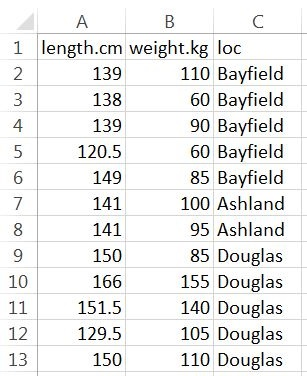
\includegraphics[width=1.5in]{Figs/Data_File_1.jpg}
\end{center}

The variable names must NOT contain any spaces.  For example use \var{len} rather than \var{total length} or \var{length (mm)}.  If you feel the need to have longer variable names, then separate the parts with a period -- e.g., \var{total.length} or an underscore \var{total\_length}.  In addition, note that numerical measurements should NOT include units -- e.g., don't use \verb"7 mm".  Finally, when using categorical data to denote group memberships make sure that all category labels are consistent.  For example, do not have a column with both \verb"male" and \verb"Male".

\warn{Variable names and data should not contain spaces.  The \R{Error in scan} error message usually indicates that you have spaces in the variable names or data.}

The Excel file should be saved as a CSV file by selecting the \verb"File..Save As" menu item which produces the following dialog box.
\begin{center}
  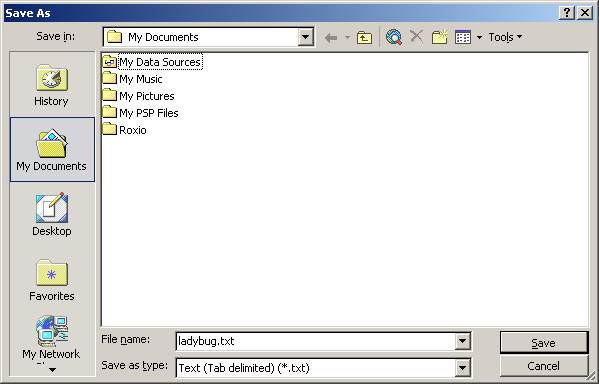
\includegraphics[width=4.5in]{Figs/Data_File_2.jpg}
\end{center}

In this dialog box change \verb"Save as type" to \verb"CSV (Comma delimited) (*.csv)" (you may have to scroll down), provide a file name (don't have any periods in the name besides ``.csv''), select a location to save the file (and don't forget this location!!), and press \verb"Save".  Two ``warning'' dialog boxes may then appear -- select \verb"OK" on the first and \verb"YES" on the second.  A CSV file will now be created with the name and in the folder you provided.  You can now close the Excel file (you will likely be asked to save changes -- you should say \verb"No").

The R working directory must be set to the directory where the the CSV file was saved before it can be read into R.  The simplest method for setting the working directory is to save an RStudio script file in the same directory as the data file.  If you do this, then you can choose the \verb"Session", \verb"Set Working Directory ...", \verb"To Source File Location" menu items in RStudio which will send an appropriate \R{setwd()} command to the R console.  This command should then be copied from the R console to your RStudio script for future use\footnote{Doing this will eliminate the need to manually select the menu options every time you want to run this script.}.

Regardless of which method you use, the result is a \R{setwd()} command that has the path to the directory containing the data as the argument.  For example, I stored the lady bug data file in the \verb"C:/data" directory.  Thus, the method of the previous paragraph would result in the following command which I then copied to my script file.

\begin{knitrout}
\definecolor{shadecolor}{rgb}{0.922, 0.922, 0.922}\color{fgcolor}\begin{kframe}
\begin{verbatim}
> setwd("C:/data/")
\end{verbatim}
\end{kframe}
\end{knitrout}

The CSV file is read into R with \R{read.csv()}.  This function requires the filename in quotes as the first argument.  For example, the CSV file of lady bug data is read into R and stored in a data frame called \var{LB} with
\begin{knitrout}
\definecolor{shadecolor}{rgb}{0.922, 0.922, 0.922}\color{fgcolor}\begin{kframe}
\begin{verbatim}
> LB <- read.table("ladybug.csv")
\end{verbatim}
\end{kframe}
\end{knitrout}

\warn{Data stored in an external CSV file is read into R with \R{read.csv()}.}

It is important that each row of the data frame correspond to one individual.  This will become critically important when data is recorded for two different groups (e.g., for a two-sample t-test; see \sectref{sect:t2test}).  For example, consider the following data of methyl mercury levels recorded in mussels from a location labeled as ``impacted'' and a separate location labeled as ``reference'',
\begin{Verbatim}
  impacted   0.011  0.054  0.056  0.095  0.051  0.077
  reference  0.031  0.040  0.029  0.066  0.018  0.042  0.044
\end{Verbatim}
To follow the ``one individual per row'' rule, these data would have to be entered in stacked format where the ``reference'' data are stacked underneath the ``impacted'' data and a column is used to indicate to which groups the individuals belong.  For example, the Excel file for data entry would look like the following

\begin{center}
  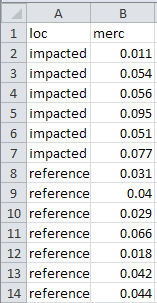
\includegraphics[width=1.5in]{Figs/StackedData.jpg}
\end{center}

\subsubsection*{Alternative Forms of Getting Data} \label{sect:RAltData}
Some of the data files that you will use are provided on the \href{http://derekogle.com/NCMTH107/resources/data_107}{Data for MTH107} resource page of the class webpage.  In these cases, the data should be downloaded from the webpage and saved in the same directory or folder as your analysis script.  The downloaded file is then read into R in the same manner as described previously (i.e., set the working direcotry with \R{setwd()} and then use \R{read.csv()}).

\warn{Every data file provided with this book contains a header and, thus, \R{header=TRUE} must be used in \R{read.table()}.}

A few data files used in this book are supplied with R or the NCStats package.  These files are installed but need to be loaded with \R{data()}.  For example, the \dfile{iris} data file is loaded into R with
\begin{knitrout}
\definecolor{shadecolor}{rgb}{0.922, 0.922, 0.922}\color{fgcolor}\begin{kframe}
\begin{verbatim}
> data(iris)
\end{verbatim}
\end{kframe}
\end{knitrout}

\section{Working With Data Frames}  \label{sect:RWorkdf}
\subsection{Viewing a Data Frame}  \label{sect:RViewdf}
Many users are disoriented in R because they cannot ``see'' their data in the same way that they see it in a spreadsheet program.  There are, however, several options for viewing your data in R.  First, you can type the name of the data frame object to see the entire contents of the data frame.  This is adequate for small data frames,
\begin{knitrout}
\definecolor{shadecolor}{rgb}{0.922, 0.922, 0.922}\color{fgcolor}\begin{kframe}
\begin{verbatim}
> fish
  len sex  dead
1  45   M  TRUE
2  56   M FALSE
3  67   F FALSE
\end{verbatim}
\end{kframe}
\end{knitrout}
but not so useful for large data frames.  The entire data frame is opened in a separate window by double-clicking on the name of the data frame in the \R{Workspace} tab of RStudio.  The first and last three rows of a data frame are viewed by including the data.frame object in \R{headtail()}.
\begin{knitrout}
\definecolor{shadecolor}{rgb}{0.922, 0.922, 0.922}\color{fgcolor}\begin{kframe}
\begin{verbatim}
> headtail(iris)
    Sepal.Length Sepal.Width Petal.Length Petal.Width   Species
1            5.1         3.5          1.4         0.2    setosa
2            4.9         3.0          1.4         0.2    setosa
3            4.7         3.2          1.3         0.2    setosa
148          6.5         3.0          5.2         2.0 virginica
149          6.2         3.4          5.4         2.3 virginica
150          5.9         3.0          5.1         1.8 virginica
\end{verbatim}
\end{kframe}
\end{knitrout}

In addition to viewing the contents of the data frame, it is often useful to examine the structure of the data frame returned from \R{str()}.  For example, the structure of the \dfile{iris} data frame is obtained with
\begin{knitrout}
\definecolor{shadecolor}{rgb}{0.922, 0.922, 0.922}\color{fgcolor}\begin{kframe}
\begin{verbatim}
> str(iris)
'data.frame':	150 obs. of  5 variables:
 $ Sepal.Length: num  5.1 4.9 4.7 4.6 5 5.4 4.6 5 4.4 4.9 ...
 $ Sepal.Width : num  3.5 3 3.2 3.1 3.6 3.9 3.4 3.4 2.9 3.1 ...
 $ Petal.Length: num  1.4 1.4 1.3 1.5 1.4 1.7 1.4 1.5 1.4 1.5 ...
 $ Petal.Width : num  0.2 0.2 0.2 0.2 0.2 0.4 0.3 0.2 0.2 0.1 ...
 $ Species     : Factor w/ 3 levels "setosa","versicolor",..: 1 1 1 1 1 1 1 1 1 1 ...
\end{verbatim}
\end{kframe}
\end{knitrout}
From this it is seen that five variables were recorded on 150 individuals.  The first four variables -- called \var{Sepal.Length}, \var{Sepal.Width}, \var{Petal.Length}, and \var{Petal.Width} -- are various numerical measurements of sepal and petals.  The last variable -- called \var{Species} -- is a factor variable that records the species of iris examined.  The levels in the \var{Species} variable are seen by including this variable (must also include the data frame name) as the argument to \R{levels()},
\begin{knitrout}
\definecolor{shadecolor}{rgb}{0.922, 0.922, 0.922}\color{fgcolor}\begin{kframe}
\begin{verbatim}
> levels(iris$Species)
[1] "setosa"     "versicolor" "virginica" 
\end{verbatim}
\end{kframe}
\end{knitrout}

\vspace{-12pt}
\subsection{Filtering a Data Frame}  \label{sect:RSubsetdf}
\vspace{-12pt}
It is common to create a new data frame that contains only some of the individuals from an existing data frame.  For example, a researcher may want to extract only the data for the \emph{setosa} species or those irises with sepal lengths greater than 5 cm from the \var{iris} data frame.  The process of creating the newer, smaller data frame is called filtering (or subsetting) and is accomplished with \R{filterD()}.  The \R{filterD()} function requires the original data frame as the first argument and a conditioning statement as the second argument.  The conditioning statement is a statement that is used to either include or exclude the individuals from the original data frame that will make up the new data frame.  The result from \R{filterD()} should be assigned an object which will then be the name of the new data frame.

\warn{The \R{filterD()} function is used to create a new data frame that consists of individuals selected by some criterion from an existing data frame.}

The conditioning statements used in \R{filterD()} can be fairly complex.  However, in this book, the conditioning statements will usually consist of the name of a variable in the original data frame, a comparison operator, and a comparison value.  Some common comparison operators are shown in \tabrefp{tab:RSubsetConditions}.

\begin{table}[htbp]
  \caption{Condition operators used in \R{filterD()} and their results.  Note that \emph{variable} generically represents a variable in the original data frame and \emph{value} is a generic value or level.  Both of these would be replaced with specific items.}  \label{tab:RSubsetConditions}
  \centering
\begin{tabular}{cc}
\hline\hline
Comparison &  \\
Operator &  Individuals Returned from Original Data Frame \\
\hline
\widen{-1}{6}{\emph{variable}} $==$ \emph{value} & all individual that are \textbf{equal} to the given value \\
\widen{-1}{5}{\emph{variable}} $!=$ \emph{value} & all individuals that are \textbf{NOT equal} to the given value \\
\widen{-1}{5}{\emph{variable}} $>$ \emph{value} & all individuals that are \textbf{greater than} the given value \\
\widen{-1}{5}{\emph{variable}} $>=$ \emph{value} & all individuals that are \textbf{greater than or equal} to the given value \\
\widen{-1}{5}{\emph{variable}} $<$ \emph{value} & all individuals that are \textbf{less than} the given value \\
\widen{-1}{5}{\emph{variable}} $<=$ \emph{value} & all individuals that are \textbf{less than or equal} to the given value \\
\widen{-1}{5}{\emph{condition}} \& \emph{condition} & all individuals that \textbf{meet both conditions} \\
\widen{-2}{6}{\emph{condition}} $|$ \emph{condition} & all individuals that \textbf{meet one or both conditions}\footnote{Note that this ``or'' operator is a ``vertical line'' which is typed with the shift-backslash key.} \\
\hline\hline
\end{tabular}
\end{table}

The following items are examples of new data frames created by subsetting the \var{iris} data frame\footnote{The \R{headtail()} function is used in these examples to show some rows in the new data frame.}.

\begin{itemize}
  \item A data frame that contains only individuals of the \emph{setosa} species\footnote{Note that in this, and all ensuing examples, that the object name to the left of the assignment operator (i.e., \R{iris.set} in this example) can be nearly any name of the authors choosing.  In other words, this object does not have to be called \R{iris.set}; it could be called nearly anything else.}.
\begin{knitrout}
\definecolor{shadecolor}{rgb}{0.922, 0.922, 0.922}\color{fgcolor}\begin{kframe}
\begin{verbatim}
> iris.set <- filterD(iris,Species=="setosa")
> headtail(iris.set)
   Sepal.Length Sepal.Width Petal.Length Petal.Width Species
1           5.1         3.5          1.4         0.2  setosa
2           4.9         3.0          1.4         0.2  setosa
3           4.7         3.2          1.3         0.2  setosa
48          4.6         3.2          1.4         0.2  setosa
49          5.3         3.7          1.5         0.2  setosa
50          5.0         3.3          1.4         0.2  setosa
\end{verbatim}
\end{kframe}
\end{knitrout}

  \item A data frame that contains individuals of the \emph{setosa} and \emph{versicolor} species.
\begin{knitrout}
\definecolor{shadecolor}{rgb}{0.922, 0.922, 0.922}\color{fgcolor}\begin{kframe}
\begin{verbatim}
> iris.setver <- filterD(iris,Species=="setosa" | Species=="versicolor")
> headtail(iris.setver)
    Sepal.Length Sepal.Width Petal.Length Petal.Width    Species
1            5.1         3.5          1.4         0.2     setosa
2            4.9         3.0          1.4         0.2     setosa
3            4.7         3.2          1.3         0.2     setosa
98           6.2         2.9          4.3         1.3 versicolor
99           5.1         2.5          3.0         1.1 versicolor
100          5.7         2.8          4.1         1.3 versicolor
\end{verbatim}
\end{kframe}
\end{knitrout}

  \item A data frame that contains individuals with a sepal length greater than 5 cm.
\begin{knitrout}
\definecolor{shadecolor}{rgb}{0.922, 0.922, 0.922}\color{fgcolor}\begin{kframe}
\begin{verbatim}
> iris.gt5 <- filterD(iris,Sepal.Length>5)
> headtail(iris.gt5)
    Sepal.Length Sepal.Width Petal.Length Petal.Width   Species
1            5.1         3.5          1.4         0.2    setosa
2            5.4         3.9          1.7         0.4    setosa
3            5.4         3.7          1.5         0.2    setosa
116          6.5         3.0          5.2         2.0 virginica
117          6.2         3.4          5.4         2.3 virginica
118          5.9         3.0          5.1         1.8 virginica
\end{verbatim}
\end{kframe}
\end{knitrout}

  \item A data frame that contains individuals of the \emph{setosa} species with a sepal length greater than 5 cm.
\begin{knitrout}
\definecolor{shadecolor}{rgb}{0.922, 0.922, 0.922}\color{fgcolor}\begin{kframe}
\begin{verbatim}
> iris.setgt5 <- filterD(iris,Species=="setosa" & Sepal.Length>5)
> headtail(iris.setgt5)
   Sepal.Length Sepal.Width Petal.Length Petal.Width Species
1           5.1         3.5          1.4         0.2  setosa
2           5.4         3.9          1.7         0.4  setosa
3           5.4         3.7          1.5         0.2  setosa
20          5.1         3.8          1.9         0.4  setosa
21          5.1         3.8          1.6         0.2  setosa
22          5.3         3.7          1.5         0.2  setosa
\end{verbatim}
\end{kframe}
\end{knitrout}
\end{itemize}

Note that after each subsetting you should either view or examine the structure of the new data frame to determine if the data frame actually contains the items that you desire.

\warn{View or ``structure'' the data frame created from using \R{filterD()} to assure that it contains data.}

\begin{exsection}
  \item \label{revex:BasicsDataFrame1} \rhw{} Two students at Seattle Community College made biometric measurements on 25 Douglas fir (\emph{Pseudotsuga menziesii}) trees in the lowlands of western Washington.  The variables recorded in the \href{https://raw.githubusercontent.com/droglenc/NCData/master/DougFirBiometrics.csv}{DougFirBiometrics.csv} file are a unique tree identifier (\var{tree}), the observer's name (\var{observer}; either ``Ingrid'' or ``Dylan''), the circumference at breast height (meters; \var{circ}), the height to the eye of the observer (meters; \var{eyeht}), the horizontal distance between observer and tree (meters; \var{horizdist}), the angle between observer and top of tree (degrees; \var{angle}), and the estimated height of tree (meters; \var{height}) using right-angle trigonometry. \ansref{ans:BasicsDataFrame1}
  \begin{Enumerate}
    \item Read this data file into an object called \R{DF}.
    \item Examine the structure of this data frame.
    \item Show all measurements made on the third tree. [Do not do this manually; use commands to find the results.]
    \item Show all estimated tree heights.
    \item Show the estimated tree height for the fifth tree.
    \item Show all measurements for all trees measured by ``Ingrid''.  [HINT: use subsetting.]
    \item Show all estimated tree heights for all trees measured by ``Dylan''.  [HINT: use subsetting.]
    \item Show all measurements for tree heights less than 10 m.  [HINT: use subsetting.]
    \item Show all measurements for tree heights greater than 10 m and circumference less than 1 m.  [HINT: use subsetting.]
  \end{Enumerate}
\end{exsection}

\newpage
\begin{hwsection}{All questions below should be typed and answered following the expectations identified in \sectref{sect:ReportWriting}.  All work must be shown.  Questions marked with the R logo must include R output with your R commands in an attached appendix.}

  \item \label{hwprob:RBasicsPL1} \rhw{} The data below are the number of purple loosestrife (\textit{Lythrum salicaria}) plants found in each of 19 randomly selected plots in the Green Gables Creek Slough.

    \begin{Verbatim}[xleftmargin=5mm]
13, 2, 1, 0, 9, 11, 5, 5, 14, 23, 0, 2, 3, 3, 6, 7, 4, 16, 1
    \end{Verbatim}

In addition, the researchers also recorded a qualitative measure of the shadiness of the plot.  The three levels of ``shadiness'' (along with abbreviations) used were ``completely shaded'' (S), ``partially shaded'' (P), and ``completely open'' (O).  The data below are the shadiness levels of the same 19 plots in the same order as the number of loosestrife plants shown above,

    \begin{Verbatim}[xleftmargin=5mm]
O,S,S,S,O,O,S,P,O,O,S,S,P,P,P,P,S,O,S
    \end{Verbatim}

Enter these data into an Excel file with columns labeled as \var{lstrf} and \var{shade}.  Save this file as a CSV file and read that file into an object called \R{df} in R.  Use this to answer the questions below using R commands (i.e., don't re-type the data).

  \begin{Enumerate}
    \item List the number of purple loosestrife plants and shadiness category for the 10th plot.
    \item List the number of purple loosestrife plants in each plot.
    \item List the data for all\footnote{Don't use \R{headtail()} when asked to show all individuals, as \R{headtail()} only shows six individuals.} of the completely shaded plots.
    \item List the data for all of the open plots.
    \item List the data for all of the completely open or partially shaded plots (use only one command in R).
    \item List the data for all plots with more than 10 purple loosestrife plants.
    \item List the data for all plots with less than 5 purple loosestrife plants and that are completely shaded (use only one command in R).
  \end{Enumerate}
\end{hwsection}

    \part{Exploratory Data Analysis}



\chapter{Univariate EDA} \label{chap:UnivEDA}
\begin{ChapObj}{\boxwidth}
  \textbf{Chapter Objectives:}
  \begin{Enumerate}
    \item Construct histograms with quantitative data,
    \item Use graphs to describe the shape of a distribution, and
    \item Use graphs to describe outliers in a distribution.
    \item Calculate summary statistics for measuring the center of quantitative data,
    \item Calculate summary statistics for measuring the dispersion of quantitative data,
    \item Describe the underlying differences in how the different statistics measure center and dispersion,
    \item Identify which summary statistics are appropriate in a given situation,
    \item Construct an appropriate overall numerical summary, and
    \item Construct frequency and percentage tables with categorical data.
    \item Construct bar-charts with categorical data, and
    \item Use tables and graphs to describe the categorical data.
  \end{Enumerate}
\end{ChapObj}

\minitoc
\newpage

\lettrine{O}{nce data have been collected} (see \chapref{chap:DataProd}), it is important to explore the distribution of the values of each variable.  The goal at this point is to develop a ``feel'' for the data, to identify what types of values each variable assumes, and to determine if there are any ``issues'' in the data.  This first step in a statistical analysis is called \textsc{Exploratory Data Analysis} (EDA).  We will begin by examining each variable by itself, called a univariate EDA, and then examine pairs of variables, called a bivariate EDA (see \chapref{chap:BivEDA}).  In addition, the methods of exploration differ for quantitative and categorical variables.  Thus, in this chapter, methods for conducting a univariate EDA with quantitative and categorical data will be described.

\section{Quantitative Univariate EDA}
A univariate EDA for quantitative data is concerned with describing the distribution of the values of a variable or, in other words, describing what values of the variable occurred and how often those values occurred.\index{EDA!Univariate!Quantitative}  Specifically, for each quantitative variable, the distribution is described by four specific attributes:

\begin{Enumerate}
  \item the \textbf{shape} of the distribution,
  \item the presence of \textbf{outliers},
  \item the \textbf{center} of the distribution, and
  \item the \textbf{dispersion} or spread of the distribution.
\end{Enumerate}

Graphs are best for identifying shape and the presence of outliers and for getting a general feel for the center and dispersion of the data.  However, numerical summaries are better for identifying the center and dispersion of the data.

\warn{Ultimately, we will describe shape, center, dispersion, and outliers of the distribution of each quantitative variable.}

\vspace{-12pt}
\warn{We will explicitly describe shape and outliers with the aid of graphs and center and dispersion with numerical summaries.}

Three primary data sets will be explored throughout this chapter.  The first data set consists of measurements of water consumption in one hour by mice \tabrefp{tab:MouseData}\footnote{See \sectref{sect:REnterData} for how to enter these data into R.}.  The second data set is the Richter scale recordings for 15 major earthquakes \tabrefp{tab:EQData}.

% latex table generated in R 3.3.1 by xtable 1.8-2 package
% Sat Aug 27 14:27:45 2016
\begin{table}[ht]
\centering
\caption{Amount of water consumed (in ml) in one hour by a sample of mice.} 
\label{tab:MouseData}
\begin{tabular}{rrrrrrrrrrrrrrr}
   \hline
10.6 & 14.1 & 13.7 & 15.2 & 15.4 & 12.5 & 12.9 & 14.3 & 13.0 & 16.6 & 11.5 & 9.4 & 16.5 & 13.7 & 14.7 \\ 
  12.6 & 12.0 & 14.0 & 10.0 & 18.2 & 18.4 & 17.4 & 11.1 & 15.8 & 15.8 & 16.6 & 11.4 & 17.0 & 13.6 & 13.5 \\ 
   \hline
\end{tabular}
\end{table}


% latex table generated in R 3.3.1 by xtable 1.8-2 package
% Sat Aug 27 14:27:45 2016
\begin{table}[ht]
\centering
\caption{Richter scale recordings for 15 major earthquakes.} 
\label{tab:EQData}
\begin{tabular}{rrrrrrrrrrrrrrr}
   \hline
5.5 & 6.3 & 6.5 & 6.5 & 6.8 & 6.8 & 6.9 & 7.1 & 7.3 & 7.3 & 7.7 & 7.7 & 7.7 & 7.8 & 8.1 \\ 
   \hline
\end{tabular}
\end{table}


The third data set is the number of days of ice cover at ice gauge station 9004 in Lake Superior (data originally\footnote{This data was found at the \href{http://www.seattlecentral.org/qelp/}{Quantitative Environmental Learning Project website}.} from the \href{http://www.nsidc.org/}{National Snow and Ice Data Center} and found in the \href{https://raw.githubusercontent.com/droglenc/NCData/master/LakeSuperiorIce.csv}{LakeSuperiorIce.csv} data file on the class webpage\footnote{See \sectref{sect:RAltData} for more description of how to access these data.}).  One variable in this file, \var{days}, is the total number of days of ice cover at this site for nearly every ice season from 1955-56 to 1996-97 (three years were missing).  These data are loaded and observed with
\begin{knitrout}
\definecolor{shadecolor}{rgb}{0.922, 0.922, 0.922}\color{fgcolor}\begin{kframe}
\begin{verbatim}
> LSI <- read.csv("data/LakeSuperiorIce.csv")
> headtail(LSI)
   season decade  temp days
1    1955   1950 22.94   87
2    1956   1950 23.02  137
3    1957   1950 25.68  106
40   1994   1990 26.63   62
41   1995   1990    NA   NA
42   1996   1990 23.88  132
\end{verbatim}
\end{kframe}
\end{knitrout}

\subsection{Histograms}\index{Histogram!Construction}\index{Sample Distribution!Histogram}
\subsubsection{General Construction}
A histogram is a plot of the frequency of occurrence of individuals (y-axis) in classes of values of the variable (x-axis).  The steps for constructing a histogram from raw data are:
\begin{Enumerate}
  \item Create categorical classes of values for the variable of interest,
  \item Count the frequency of individuals in each class,
  \item Construct a graph template with values of the variable on the x-axis and frequency of individuals on the y-axis, and
  \item Draw bars on the graph that are as wide as the class of values and as tall as the frequency of individuals.
\end{Enumerate}
These steps will be illustrated below with the mouse water consumption data.

The first step is to create a list of classes of the water consumption data.  The easiest way to do this by hand is to find the difference between the maximum and minimum value in the data set and divide this value by the number of desired bars.  The number of bars is usually a ``nice'' number near eight to ten.  This number is typically rounded up to make classes that are easy to work with.  The range of values in this example is 18.4-9.4 = 9.0.  A ``nice'' value between eight and ten to divide the range by in this example is nine.  Thus, the classes of data should be one unit wide.  To make the histogram as easy as possible to construct by hand it is best to start the classes at 9 mm \tabrefp{tab:MouseFreqTable}.

\begin{table}[htbp]
  \caption{Frequency table of mouse consumption values in one-unit classes.}
  \label{tab:MouseFreqTable}
    \begin{Verbatim}[xleftmargin=5mm]
Class     Frequency
 9.0- 9.9      1
10.0-10.9      2
11.0-11.9      3
12.0-12.9      4
13.0-13.9      5
14.0-14.9      4
15.0-15.9      4
16.0-16.9      3
17.0-17.9      2
18.0-18.9      2
    \end{Verbatim}
\end{table}

The next step is to count the number of individuals with a value of the variable in each class.  These values are called the frequencies and are shown in the second column of \tabref{tab:MouseFreqTable}.

We now prepare a plot for placing the frequency data on.  The values of the classes will form the x-axis and the frequencies will form the y-axis (\figref{fig:MouseHist1}-Left).  To this skeleton plot a bar is added with the left-bottom corner at 9 and the right-bottom corner at 10 on the x-axis and with a height equal to the frequency of individuals in the 9 to 9.9 class (\figref{fig:MouseHist1}-Center).  A second bar is then added with the left-bottom corner at 10 and the right-bottom corner at 11 on the x-axis and with a height equal to the frequency of individuals in the 10 to 10.9 class (\figref{fig:MouseHist1}-Right).  This process is continued with the remaining classes until the full histogram is constructed \figrefp{fig:MouseHist2}.

\begin{knitrout}
\definecolor{shadecolor}{rgb}{0.922, 0.922, 0.922}\color{fgcolor}\begin{figure}[hbtp]

{\centering 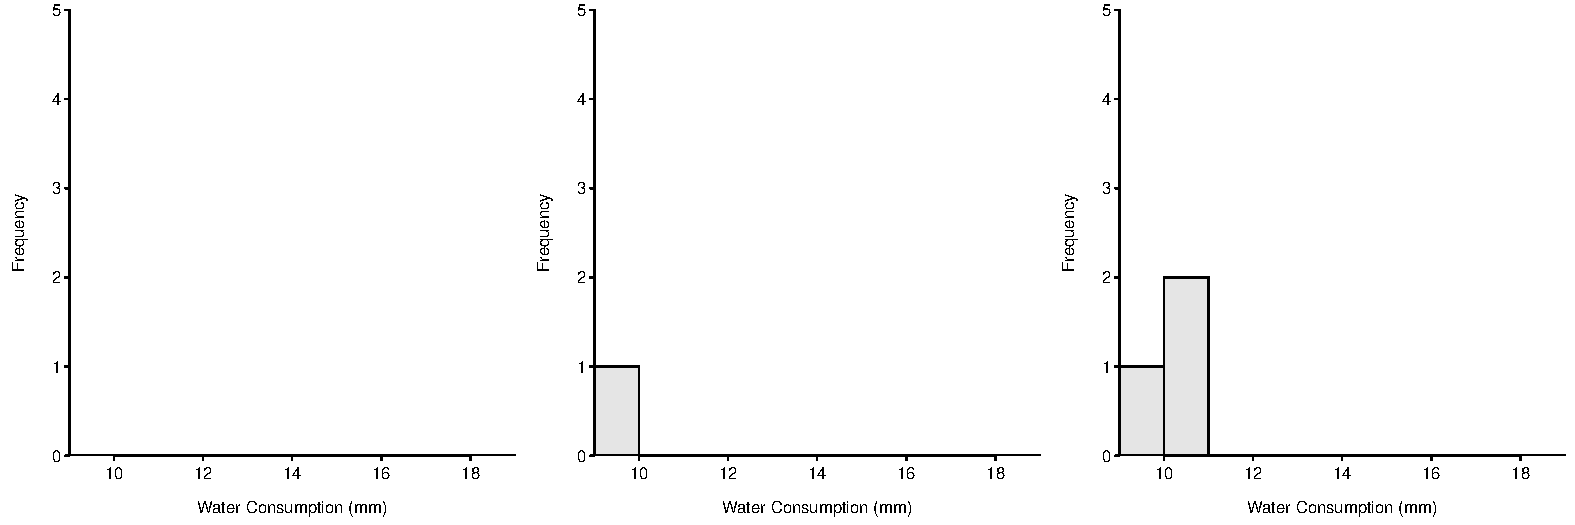
\includegraphics[width=.95\linewidth]{Figs/MouseHist1-1} 

}

\caption[Steps illustrating the development of a histogram]{Steps illustrating the development of a histogram.}\label{fig:MouseHist1}
\end{figure}


\end{knitrout}

\vspace{24pt}  % handles an overlapping problem with the floats

\begin{knitrout}
\definecolor{shadecolor}{rgb}{0.922, 0.922, 0.922}\color{fgcolor}\begin{figure}[hbtp]

{\centering 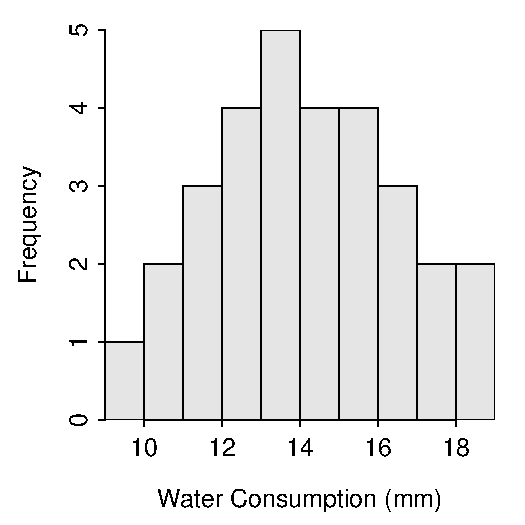
\includegraphics[width=.4\linewidth]{Figs/MouseHist2-1} 

}

\caption[Histogram of water consumption (mm) by mice]{Histogram of water consumption (mm) by mice.}\label{fig:MouseHist2}
\end{figure}


\end{knitrout}

Ideally eight to ten classes (i.e., bars) are used to construct a histogram.  Too many or too few bars make it difficult to identify the shape and may lead to different interpretations.  A dramatic example of the effect of changing the number of classes is seen in a series of histograms of the length of eruptions for the Old Faithful geyser \figrefp{fig:histOF}.

\begin{knitrout}
\definecolor{shadecolor}{rgb}{0.922, 0.922, 0.922}\color{fgcolor}


















































\begin{figure}[hbtp]

{\centering \animategraphics[width=.4\linewidth,controls,palindrome,autoplay]{1}{Figs/histOF-}{1}{52}

}

\caption[Hisgoram of length (minutes) of eruprtions for Old Faitfhul geyser with varying number of classes]{Hisgoram of length (minutes) of eruprtions for Old Faitfhul geyser with varying number of classes.}\label{fig:histOF}
\end{figure}


\end{knitrout}

\subsubsection{Histograms in R}
Histograms are constructed with \R{hist()} with a one-side formula of the form \R{\TILDE quant} where \R{quant} generically represents the quantitative variable and the \R{data=} argument.  For example, \R{hist(\TILDE days,data=LSI)} produces the default plot shown on the left of \figref{fig:Histogram1}.  A more proper histogram would not have the main title above the histogram and the x-axis would be labeled in a more readable manner.  The main title is removed by including the \R{main=""} argument\footnote{\R{main=} is for the ``main'' title.}.  The x-axis label is improved by including the \R{xlab="Days of Ice Cover"} argument\footnote{\R{xlab=} is for the ``x-axis label.''}.  The histograms in \figref{fig:Histogram1} are produced with

\begin{knitrout}
\definecolor{shadecolor}{rgb}{0.922, 0.922, 0.922}\color{fgcolor}\begin{kframe}
\begin{verbatim}
> hist(~days,data=LSI)                                    # Left
> hist(~days,data=LSI,main="",xlab="Days of Ice Cover")   # Right
\end{verbatim}
\end{kframe}\begin{figure}[hbtp]

{\centering 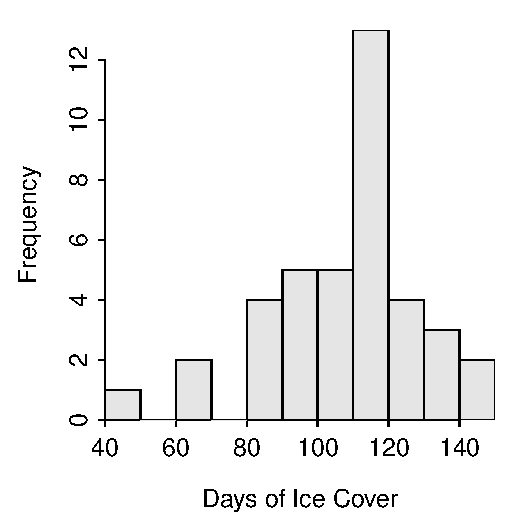
\includegraphics[width=.4\linewidth]{Figs/Histogram1-1} 
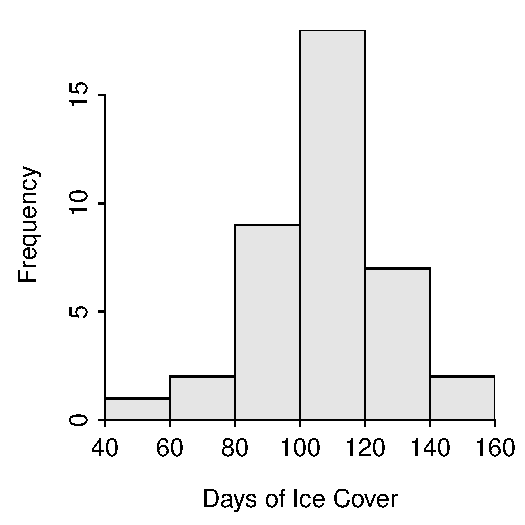
\includegraphics[width=.4\linewidth]{Figs/Histogram1-2} 

}

\caption[Histograms of the duration of ice cover at ice gauge 9004 in Lake Superior]{Histograms of the duration of ice cover at ice gauge 9004 in Lake Superior.}\label{fig:Histogram1}
\end{figure}


\end{knitrout}

\warn{The default histogram should be modified by removing the main graph label and properly labeling the x-axis.}

The number of bins or classes is modified with the \R{breaks=} argument.  The endpoints for the bin values are set by setting the \R{breaks=} argument to a vector of endpoints\footnote{The default bins are left-inclusive and right-exclusive.  In other words, the bins have the form $[a,b)$ where the value of $a$ would be in the bin but the value of $b$ would no be.  For example, the bin $[20,40)$ would include an individual with a value of $20$ but not an individual with a value of $40$.  The bins are changed to left-inclusive and right-exclusive, i.e., $(a,b]$, by including the \R{right=TRUE} option as an argument in \R{hist()}.  Typically, this is not an important distinction because only very broad conclusions are of interest when performing an EDA.  However, this argument may be important when handling discrete data.}.  For example, the histograms shown in \figref{fig:Histogram2} was created by controlling the bin values with

\begin{knitrout}
\definecolor{shadecolor}{rgb}{0.922, 0.922, 0.922}\color{fgcolor}\begin{kframe}
\begin{verbatim}
> hist(~days,data=LSI,main="",xlab="Days of Ice Cover",breaks=c(40,60,80,100,120,140,160))
\end{verbatim}
\end{kframe}\begin{figure}[hbtp]

{\centering \includegraphics[width=.4\linewidth]{Figs/Histogram2-1} 

}

\caption[Histogram of the duration of ice cover at ice gauge 9004 in Lake Superior showing classes defined by the \R{c(40,60,80,100,140,180)} vector]{Histogram of the duration of ice cover at ice gauge 9004 in Lake Superior showing classes defined by the \R{c(40,60,80,100,140,180)} vector.}\label{fig:Histogram2}
\end{figure}


\end{knitrout}

\newpage % may not need upon revision, forces title to be with questions
\begin{exsection}
  \item \label{revex:quEDAHistVar} Histograms are constructed from what type of variables? \ansref{ans:quEDAHistVar}
  \item \label{revex:quEDAHistX} What type of values are plotted on the x-axis of a histogram? \ansref{ans:quEDAHistX}
  \item \label{revex:quEDAHistY} What type of values are plotted on the y-axis of a histogram? \ansref{ans:quEDAHistY}
  \item \label{revex:quEDAHistBins} What is the ideal number of bars on a histogram? \ansref{ans:quEDAHistBins}
  \item \label{revex:quEDACreatPhosph} \rhw{} The table below contains the concentrations (International Units per liter) of creatine phosphokinase (an enzyme related to muscle and brain functions) in 36 male volunteers.  Construct a histogram from these data.  [HINT: Enter these data into Excel and load into R as described in \sectref{sect:REnterData}.]\ansref{ans:quEDACreatPhosph}
    \begin{Verbatim}[xleftmargin=5mm]
121  82 100 151  68  58  95 145  64 119 104 110 113 118 203  62  83  67
201 101 163  84  57 139  60  78  94  93  92 110  25 123  70  48  95  42
    \end{Verbatim}
  \item \label{revex:quEDAAirPolln} \rhw{} The table below contains the carbon monoxide levels (ppm) arising from one of the stacks for an oil refinery northeast of San Francisco between April 16 and May 16, 1993. The measurements were submitted as evidence for establishing a baseline to the Bay Area Air Quality Management District (BAAQMD)\footnote{BAAQMD personnel had also made nine independent measurements of the carbon monoxide from this same stack over the period from September 11, 1990, to March 30, 1993, (which are not shown).}.  Construct a histogram from these data.  [HINT: Enter these data into Excel and load into R as described in \sectref{sect:REnterData}.]\ansref{ans:quEDAAirPolln}
    \begin{Verbatim}[xleftmargin=5mm]
30 30 34 36 37 38 40 42 43  43  45  52  55  58 58 58
59 63 63 71 75 85 86 86 99 102 102 141 153 261 21
    \end{Verbatim}
\end{exsection}

\subsection{Interpreting Shape}\index{Histogram!Interpretation}
A histogram has two tails -- a left-tail for smaller or more negative values and a right-tail for larger or more positive values.  The relative appearance of these two tails is used to identify three different shapes of distributions -- symmetric, left-skewed, and right-skewed.\index{Shape}\index{Symmetric}\index{Skewed}  If the left- and right-tail of a histogram are equal in shape (length and height), then the distribution is said to be \textbf{symmetric}.  Perfectly symmetric distributions rarely occur in ``real-life.''  Therefore, if the left- and right-tail are approximately equal in shape, then the distribution is \textbf{approximately symmetric}.  If the left-tail of the histogram is stretched out or, alternatively, the left-tail is longer and flatter than the right-tail, then the distribution is negatively- or \textbf{left-skewed}.  If the right-tail of the histogram is stretched out or, alternatively, the right-tail is longer and flatter than the left-tail, then the distribution is positively- or \textbf{right-skewed}.  The type of skew is defined by the longer tail; a longer right-tail means the distribution is right-skewed and a longer left-tail means it is left-skewed.  Examples of each shape are shown in \figref{fig:ShapeExamples}.

\begin{knitrout}
\definecolor{shadecolor}{rgb}{0.922, 0.922, 0.922}\color{fgcolor}\begin{figure}[hbtp]

{\centering 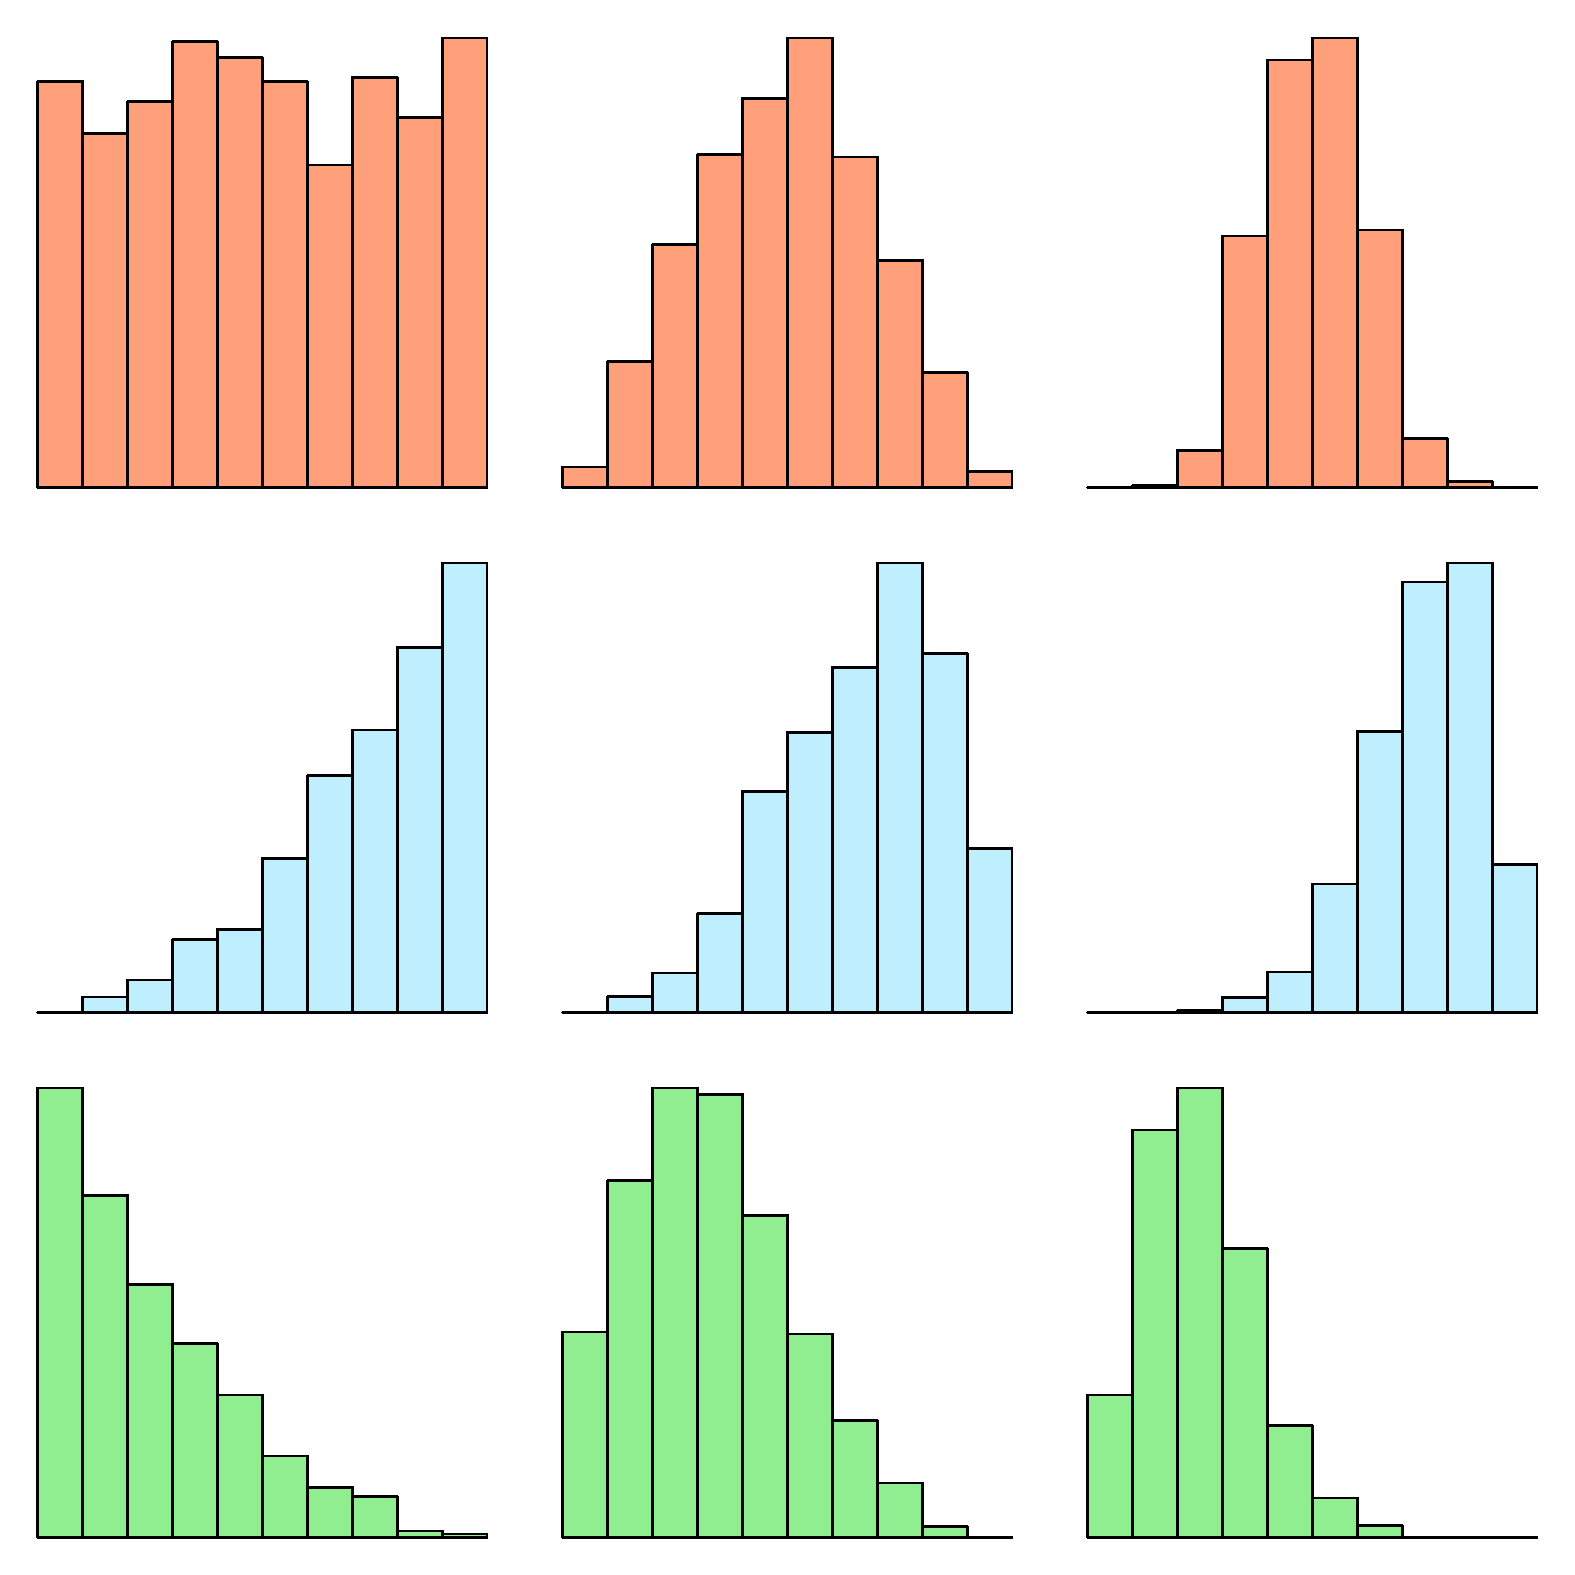
\includegraphics[width=.7\linewidth]{Figs/ShapeExamples-1} 

}

\caption[Examples of approximately symmetric (top, red), left-skewed (middle, blue), and right-skewed (bottom, green) histograms]{Examples of approximately symmetric (top, red), left-skewed (middle, blue), and right-skewed (bottom, green) histograms.  Note that the axes labels were removed to focus attention on the shape of the histograms.  Each histogram was constructed from n=1000 individuals and the x-axis range is from 0 to 1.}\label{fig:ShapeExamples}
\end{figure}


\end{knitrout}

\defn{Symmetric}{The left- and right-tail of a distribution are nearly the same in length and height.}

\vspace{-12pt}
\defn{Left-skewed}{The left-tail of a distribution is longer or more drawn out than the right-tail.}

\vspace{-12pt}
\defn{Right-skewed}{The right-tail of a distribution is longer or more drawn out than the left-tail.}

\vspace{-12pt}
\warn{The longer tail defines the type of a skewed distribution.}

You will find in practice that these labels form a continuum.  For example, a perfectly symmetric distribution is rare.  However, in the many cases of an asymmetric distribution, it is a fine line between calling the shape approximately symmetric or one of the skewed distributions.

\warn{Symmetric, left-skewed, and right-skewed descriptors are guides; many ``real'' distributions will not fall neatly into these categories.}


\subsection{Interpreting Outliers}\index{Outlier}\index{Histogram!Interpretation}
An outlier is an individual in a sample whose value is widely separated from the main cluster of values in the sample.  On histograms, outliers appear as bars that are separated from the main cluster of bars by ``white space'' or areas with no bars \figrefp{fig:OutlierExHist}.  In general, outliers must be on the margins of the histogram, should be separated by one or two missing bars, and should only be one or two individuals.

\begin{knitrout}
\definecolor{shadecolor}{rgb}{0.922, 0.922, 0.922}\color{fgcolor}\begin{figure}[hbtp]

{\centering 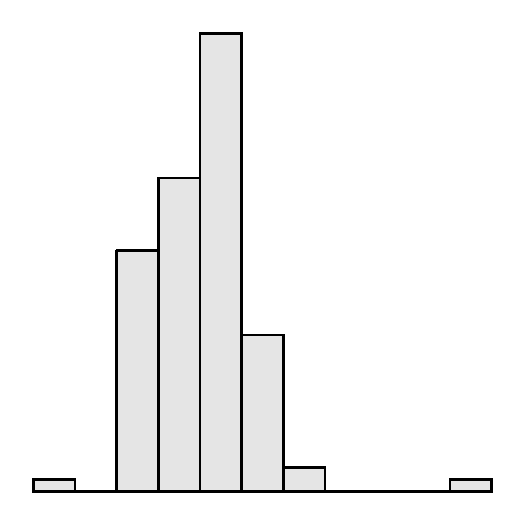
\includegraphics[width=.4\linewidth]{Figs/OutlierExHist-1} 

}

\caption[Example histogram with an outlier to the right]{Example histogram with an outlier to the right.}\label{fig:OutlierExHist}
\end{figure}


\end{knitrout}

\defn{Outlier}{An individual in a sample whose value is widely separated from the main cluster of values in the sample.}

\vspace{-12pt}
\warn{In general, don't consider a group of more than two individuals as outliers even if they are separated from the main cluster of individuals.}

Outliers are not necessarily evil.  Sometimes outliers do occur as a result of human error in the sampling process.  If this is the case, then the individual's value should be corrected or removed.  Sometimes outliers are individuals that are not part of the population of interest -- e.g., an adult animal that was sampled when only immature animals were being considered.  In this case, the individual's value should be removed from the sample.  Sometimes outliers are simply part of the population.  In this case you should generally not remove the individual's value; in fact you may wish to highlight its existence as an interesting observation.  In any case, it is important that you plot the distribution of your data with a histogram to determine if outliers are present or not.

Don't let outliers completely influence how you define the shape of a distribution.  For example, if the main cluster of values is approximately symmetric and there is one outlier to the right of the main cluster (as illustrated in \figref{fig:OutlierExHist}), \textbf{DON'T} call the distribution right-skewed.  You should describe this distribution as approximately symmetric with an outlier to the right.

\warn{Not all outliers warrant removal from your sample.}

\vspace{-12pt}
\warn{Don't let outliers completely influence how you define the shape of a distribution.}

Graphing data is the first step in an EDA and is used to identify the shape and presence of outliers.  In the next several pages numerical summaries of center and dispersion will be introduced.


\vspace{24pt}
\begin{exsection}
  \item \label{revex:quEDALSkew} What is a distribution with a long left-tail called? \ansref{ans:quEDALSkew}
  \item \label{revex:quEDARSkew} What is a distribution with a long right-tail called? \ansref{ans:quEDARSkew}
  \item \label{revex:quEDALSkewg} What is the shape of the distribution on the left below? \ansref{ans:quEDALSkewg}


\begin{center}
  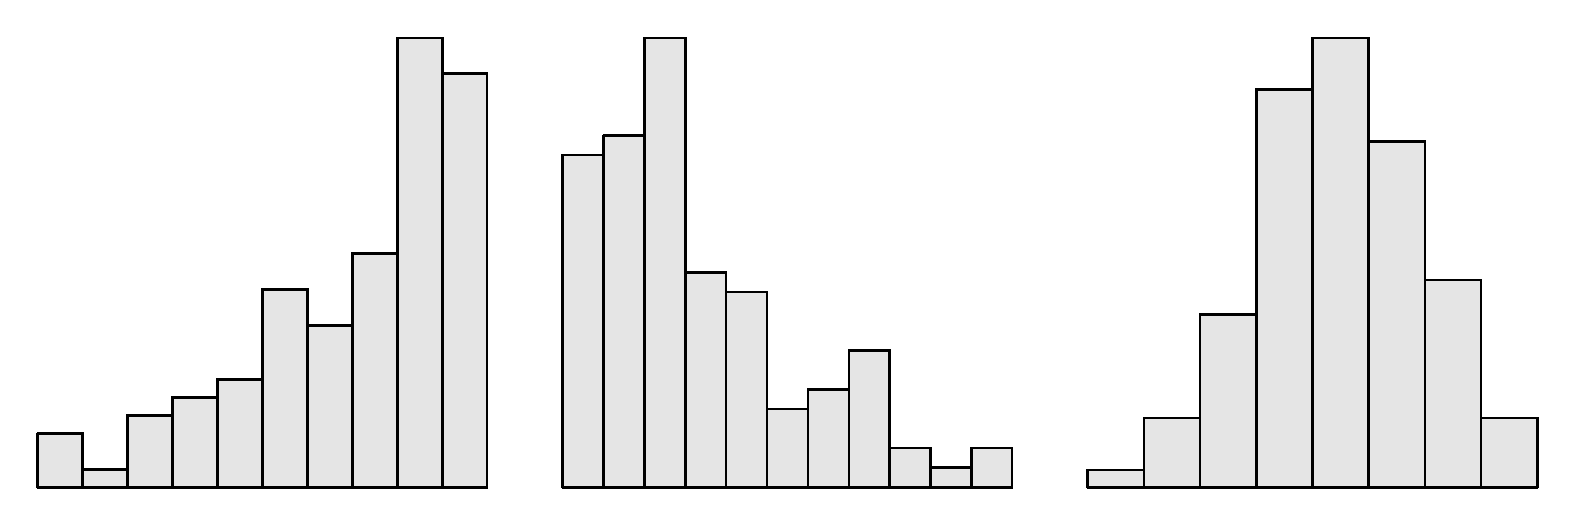
\includegraphics[width=5in]{Figs/HistQuest-1}
\end{center}
  \item \label{revex:quEDASymg} What is the shape of the distribution in the center above? \ansref{ans:quEDASymg}
  \item \label{revex:quEDARSkewg} What is the shape of the distribution on the right above? \ansref{ans:quEDARSkewg}
  \item \label{revex:quEDAlead} Comment on the shape and presence of outliers in \figref{fig:KreherParkPbhist}. \ansref{ans:quEDAlead}
\end{exsection}


\subsection{Measures of Center} \label{sec:quEDACenter}
There are three common methods to measure the center of a distribution: the mode, median, and mean.\index{Center}  The median and mean are the most widely used methods.  The choice of which method to use depends, in part, on the shape of the distribution, the presence of outliers, and your purpose.

The modes, medians, and means computed in this section are summary statistics -- i.e., they are computations from individuals in a sample.  Thus, they should specifically be called the sample mode, sample median, and sample mean.  The mode, median, and mean can also be computed from every individual in the population, if it is known.  The computed values would then be parameters and should be called the population mode, population median, and population mean.  For clarification on the differences between populations and samples and parameters and statistics, consult \sectref{sect:IVPPSS}.

\warn{Three measures of the center of a distribution are the mode, median, and mean.}

\vspace{12pt}
\warn{Measures of center computed from individuals in a sample are preceded by the word ``sample''; those computed from all individuals in a population are preceded by the word ``population.''}

\subsubsection{Mode}
The mode is the value that occurs most often in a data set.\index{Mode}  If the variable is continuous, then the modal class is the class of values that occurs most often in a data set.  In other words, it is the class that is the peak of a distribution.  For example, in the mouse water consumption data \figrefp{fig:MouseHist2} the modal class is the 13.0-13.9 class.  Some data sets may have what looks like two ``humps.''  Each ``hump'' is considered a mode and the distribution is said to be \textbf{bimodal}.

\defn{Mode}{The value or class of values that occurs most often in a data set.}

\vspace{-12pt}
\defn{Bimodal}{The shape of a distribution with two peaks or ``humps.''}

\subsubsection{Mean}
The mean is the arithmetic average of the data.\index{Mean!Calculation}  The sample mean is denoted by $\bar{x}$ and the population means is denoted by $\mu$.\index{Mean!Sample Symbol}\index{Mean!Population Symbol}  If the measurement of the generic variable $x$ on the $i$th individual is denoted as $x_{i}$, then the sample mean is computed with these two steps,
\begin{Enumerate}
  \item Sum (i.e., add together) all of the values -- $\Sum_{i=1}^{n}x_{i}$.
  \item Divide by the number of individuals in the sample -- $n$.
\end{Enumerate}
or, more succinctly, summarized with this equation,

\begin{equation} \label{eqn:SampleMean}
     \bar{x} = \frac{\Sum_{i=1}^{n}x_{i}}{n}
\end{equation}

For example, the sample mean of the mouse consumption data is computed as follows:

\[ \bar{x} = \frac{9.4+10.0+10.6+11.1+11.4+11.5+ ... +16.6+16.6+17.0+17.4+18.2}{30} = \frac{421.2}{30} = 14.04  \]

\defn{Mean}{The center of gravity or balance point of the data, i.e., the sum of the data divided by the number of individuals}.

\subsubsection{Median} \label{sec:Median}
The median is the value of the individual in the position that splits the \textbf{ordered} list of individuals into two equal-\textbf{sized} halves.\index{Median!Calculation}  In other words, if the data are ordered, half the values will be smaller than the median and half will be larger.

The process for finding the median consists of three steps\footnote{Most computer programs use a more sophisticated algorithm for computing the median and, thus, will produce different results than what will result from applying these steps.},
\begin{Enumerate}
  \item Order the data from smallest to largest.
  \item Determine what \textbf{position} the median ($mp$)\footnote{$mp$ stands for ``the middle position.''} is in with $mp=\frac{n+1}{2}$.
  \item If $mp$ is an integer (i.e., no decimal), then the median is the value of the individual in that position.  If $mp$ is not an integer, then the median is the average of the value immediately below and the value immediately above the $mp$.
\end{Enumerate}

As an example, examine the mouse water consumption data from \tabref{tab:MouseData}.  The ordered data are,

% latex table generated in R 3.3.1 by xtable 1.8-2 package
% Sat Aug 27 14:27:45 2016
\begin{tabular}{rrrrrrrrrrrrrrr}
  9.4 & 10.0 & 10.6 & 11.1 & 11.4 & 11.5 & 12.0 & 12.5 & 12.6 & 12.9 & 13.0 & 13.5 & 13.6 & 13.7 & 13.7 \\ 
  14.0 & 14.1 & 14.3 & 14.7 & 15.2 & 15.4 & 15.8 & 15.8 & 16.5 & 16.6 & 16.6 & 17.0 & 17.4 & 18.2 & 18.4 \\ 
  \end{tabular}


Because $n=30$, the $mp=\frac{30+1}{2}=15.5$.  The $mp$ is not an integer so the median is the average of the values in the 15th and 16th ordered positions (i.e., the two actual positions closest to $mp$).  Thus, the median water consumption in this sample of mice is $\frac{13.7+14.0}{2}=13.85$ mm.

As another example, consider finding the median of the Richter Scale magnitude recorded for fifteen major earthquakes \tabrefp{tab:EQData}.  Because $n=15$, the $mp=\frac{15+1}{2}=8$.  The $mp$ is an integer (i.e., no decimals) so the median is the value of the individual that is in the 8th ordered position which is 7.1 (note that the data presented in \tabref{tab:EQData} was already ordered).

\defn{Median}{The midpoint of the data, i.e., the value of the individual in the position that splits the ordered list of individuals into two equal-sized halves.}


\subsection{Measures of Center in R} \label{sect:DescStatsCenter}\index{Mean!Calculation}\index{Median!Calculation}
\vspace{-12pt}
The mean and median (along with other measures) are calculated in R with \R{Summarize()} using a one-side formula of the form \R{\TILDE quant}, where \R{quant} generically represents the quantitative variable, and the \R{data=} argument.  However, you can control the number of digits after the decimal place with the \R{digits=} argument.  Thus, all of the descriptive statistics for the duration of ice cover are computed with
\begin{knitrout}
\definecolor{shadecolor}{rgb}{0.922, 0.922, 0.922}\color{fgcolor}\begin{kframe}
\begin{verbatim}
> Summarize(~days,data=LSI,digits=2)
       n   nvalid     mean       sd      min       Q1   median       Q3      max 
   42.00    39.00   107.85    21.59    48.00    97.00   114.00   118.00   146.00 
percZero 
    0.00 
\end{verbatim}
\end{kframe}
\end{knitrout}

From this we see that the sample mean is 107.85 and the sample median is 114.00.

\begin{exsection}
  \item \label{revex:quEDABrule} \rhw{} The following values are the maximum gauge heights of the Bois Brule River in Brule, WI from 10-25Feb05\footnote{Data collected from \href{http://waterdata.usgs.gov/wi/nwis/uv?04025500}{USGS}.}.  Compute the mean and median of these data both ``by hand'' and with R.  [HINT: Enter these data into Excel and load into R as described in \sectref{sect:REnterData}.] \ansref{ans:quEDABrule}
  \begin{Verbatim}[xleftmargin=5mm]
1.56 1.54 1.54 1.57 1.58 1.61 1.60 1.69
1.99 2.11 1.98 1.76 1.69 1.99 1.86 1.53
  \end{Verbatim}

  \item \label{revex:quEDAWIc} \rhw{} The following values are the population density (number of people per acre of land) for 15 randomly selected Wisconsin counties\footnote{Data collected from \href{http://factfinder.census.gov/}{U.S. census}.}.  Compute the mean and median of these data both ``by hand'' and with R.  [HINT: Enter these data into Excel and load into R as described in \sectref{sect:REnterData}.]\ansref{ans:quEDAWIC}
  \begin{Verbatim}[xleftmargin=5mm]
429.0  67.8  52.1  97.4  57.9 354.9  16.2  19.1
127.0  27.6  10.2  54.6  28.8  30.1  20.2
  \end{Verbatim}

  \item \label{revex:quEDACreatPhosph2} \rhw{} Compute the mean and median of the creatine phosphate data in Exercise \ref{revex:quEDACreatPhosph}. \ansref{ans:quEDACreatPhosph2}

    \item \label{revex:quEDAAirPolln2} \rhw{} \hspace{12pt} Compute the mean and median of the carbon monoxide data in Exercise \ref{revex:quEDAAirPolln}. \ansref{ans:quEDAAirPolln2}
\end{exsection}

\subsection{Comparing the Median and Mean} \label{sect:MeanMedian}
The mean and median measure center in different ways.\index{Median!Compared to mean}\index{Mean!Compared to median}\index{Mean!How measures center}\index{Median!How measures center}  The median is concerned with the \textbf{position} of the value rather than the value itself (recall how it is calculated).  The mean, on the other hand, is the value such that the sum of the distances from it to all points smaller than it is the same as the sum of the distances from it to all points greater than it.  The mean is very much concerned about the \textbf{values} for each individual as the values are used to find the ``distance'' from the mean.

\warn{The actual values of the data (beyond ordering the data) are not considered when calculating the median; whereas the actual values are very much considered when calculating the mean.}

A plot of the earthquake Richter scale data against the corresponding ordered individual number is shown in \figref{fig:MeanMedianComp1}-Left \footnote{This is a rather non-standard graph but it is useful for comparing how the mean and median measure the center of the data.}.  The median (blue line) is found by locating the middle position on the individual number axis and then finding the corresponding Richter scale value (move right until the point is intercepted and then move down to the x-axis).  The vertical blue line represents the median, and it can be seen that it has the same \textbf{number} of individuals (i.e., points) below it as above it.  In contrast, the mean finds the Richter scale value that has the same total distance to values below it as total distance to values above it.  In other words, the mean is the vertical red line so that the total \textbf{length} of the horizontal dashed red lines is the same to the left as it is to the right.  Thus, the median balances the number of individuals above and below the median whereas the mean balances the difference in values above and below the mean.

\begin{knitrout}
\definecolor{shadecolor}{rgb}{0.922, 0.922, 0.922}\color{fgcolor}\begin{figure}[hbtp]

{\centering 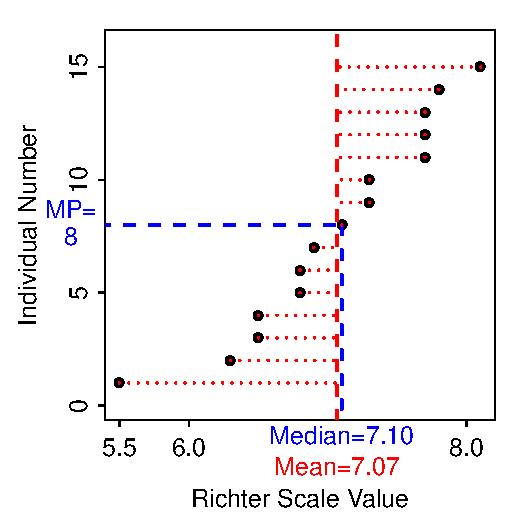
\includegraphics[width=.45\linewidth]{Figs/MeanMedianComp1-1} 
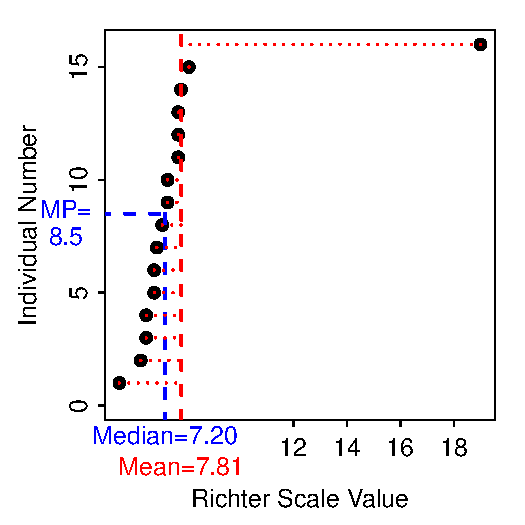
\includegraphics[width=.45\linewidth]{Figs/MeanMedianComp1-2} 

}

\caption[Plot of the individual number versus Richter scale values for the original earthquake data (\textbf{Left}) and the earthquake data with an extreme outlier (\textbf{Right})]{Plot of the individual number versus Richter scale values for the original earthquake data (\textbf{Left}) and the earthquake data with an extreme outlier (\textbf{Right}).  The median value is shown as a blue vertical line and the mean value is shown as a red vertical line.  Differences between each individual value and the mean value are shown with horizontal red lines.}\label{fig:MeanMedianComp1}
\end{figure}


\end{knitrout}

\warn{The mean balances the distance to individuals above and below the mean. The median balances the number of individuals above and below the median.}

\vspace{-12pt}
\warn{The sum of all differences between individual values and the mean (as properly calculated) equals zero.}

The mean and median differ in their sensitivity to outliers (\figref{fig:MeanMedianComp1}-Right).\index{Mean!Sensitivity to outliers}\index{Median!Sensitivity to outliers}  For example, suppose that an incredible earthquake with a Richter Scale value of 19.0 was added to the earthquake data set.  With this additional individual, the median increases from 7.1 to 7.2, but the mean increases from 7.1 to 7.8.  The outlier affects the value of the mean more than it affects the value of the median because of the way that each statistic measures center.  The mean will be pulled towards an outlier because it must ``put'' many values on the ``side'' of the mean away from the outliers so that the sum of the differences to the larger values and the sum of the differences to the smaller values will be equal.  Thus, the outlier in this example creates a large difference to the right of the mean so the mean has to ``move'' to the right to make this difference smaller, move more individuals to the left side of the mean, and increase the differences of individuals to the left of the mean to balance this one large individual.  The median on the other hand will simply ``put'' one more individual on the side opposite of the outlier because it balances the number of individuals on each side of it.  Thus, the median has to move very little to the right to accomplish this balance.

\warn{The mean is more sensitive (i.e., changes more) to outliers than the median; it will be ``pulled'' towards the outlier more than the median.}

The shape of the distribution, even if outliers are not present, also has an effect on the values of the mean and median as depicted in \figref{fig:MeanMedianShape}.  If a distribution is perfectly symmetric, then the median and mean (along with the mode) will be identical.  If the distribution is approximately symmetric, then the median and mean will be approximately equal.  If the distribution is right-skewed, then the mean will be greater than the median.  Finally, if the distribution is left-skewed, then the mean will be less than the median.

\begin{knitrout}
\definecolor{shadecolor}{rgb}{0.922, 0.922, 0.922}\color{fgcolor}\begin{figure}[hbtp]

{\centering 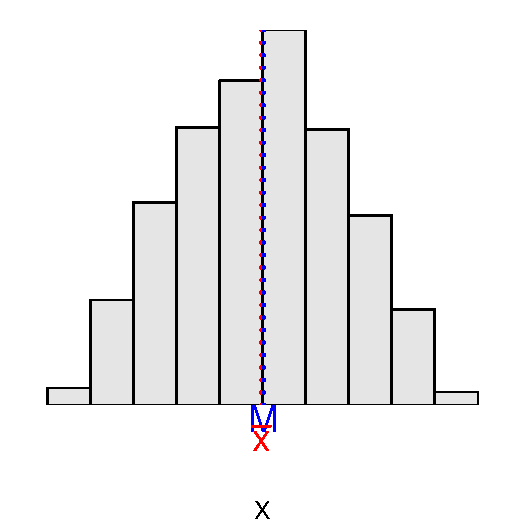
\includegraphics[width=.3\linewidth]{Figs/MeanMedianShape-1} 
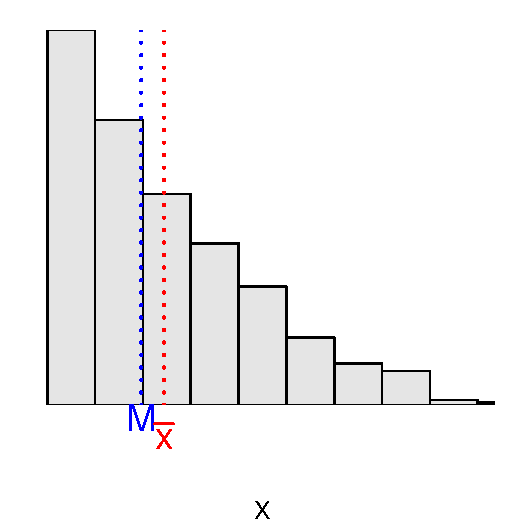
\includegraphics[width=.3\linewidth]{Figs/MeanMedianShape-2} 
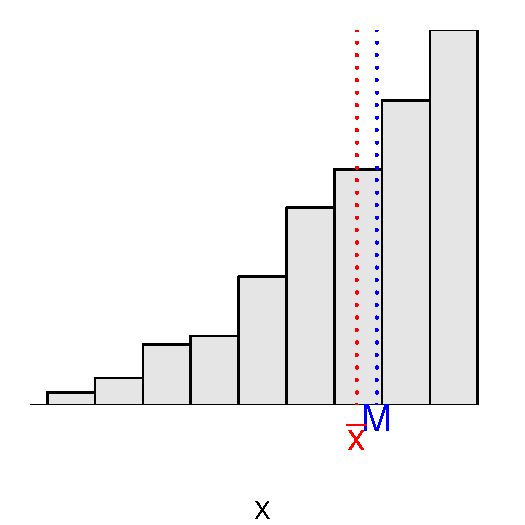
\includegraphics[width=.3\linewidth]{Figs/MeanMedianShape-3} 

}

\caption[Three differently shaped histograms with vertical lines superimposed at the median (M]{Three differently shaped histograms with vertical lines superimposed at the median (M; blue lines) and the mean ($\bar{x}$; red lines).}\label{fig:MeanMedianShape}
\end{figure}


\end{knitrout}

\warn{The mean and median are equal for symmetric distributions.}

\vspace{-12pt}
\warn{The mean is pulled towards the long tail of a skewed distribution. Thus, the mean is greater than the median for right-skewed distributions and the mean is less than the median for left-skewed distributions.}

As shown above, the mean and median measure center in different ways.  The question now becomes ``which measure of center is better?''  The median is a ``better'' measure of center when outliers are present.  In addition, when the data are skewed the median gives a better measure of a typical individual.  Thus, in this book let us agree to use the median when outliers are present or the distribution of the data is skewed.\index{Median!When to use}  If the distribution is symmetric, then the purpose of the analysis will dictate which measure of center is ``better.''  However, in this course, let us also agree to use the mean when the data are symmetric or, at least, not strongly skewed.\index{Mean!When to use}

\warn{Describe center with the median if outliers are present or the data are skewed; use the mean if the data are symmetric and no outliers are present.}


\begin{exsection}
  \item \label{revex:quEDALSkewMM}Is the mean less than, approximately equal to, or greater than the median for the distribution shown in Exercise \ref{revex:quEDALSkewg}? \ansref{ans:quEDALSkewMM}
  \item \label{revex:quEDAAsymMM}Is the mean less than, approximately equal to, or greater than the median for the distribution shown in Exercise \ref{revex:quEDASymg}? \ansref{ans:quEDAAsymMM}
  \item \label{revex:quEDARSkewMM}Is the mean less than, approximately equal to, or greater than the median for the distribution shown in Exercise \ref{revex:quEDARSkewg}? \ansref{ans:quEDARSkewMM}
  \item \label{revex:quEDARatio} Is the mean divided by the median less than 1, equal to 1, or greater than 1 for a symmetric distribution? \ansref{ans:quEDARatio}
  \item \label{revex:quEDABruleMM} From your calculation of the mean and median in Review Exercise  \ref{revex:quEDABrule} do you expect the histogram to be left-skewed, approximately symmetric, or right-skewed? \ansref{ans:quEDABruleMM}
  \item \label{revex:quEDAWIcMM} From your calculation of the mean and median in Review Exercise \ref{revex:quEDAWIc} do you expect the histogram to be left-skewed, approximately symmetric, or right-skewed? \ansref{ans:quEDAWIcMM}
\end{exsection}


\subsection{Measures of Dispersion}
There are three common methods for measuring the dispersion of a distribution: the range, inter-quartile range (IQR), and standard deviation.\index{Dispersion}  The standard deviation is the most widely used method.  The choice of which method to use depends, however, on what statistic you chose as the measure of center and, thus, depends on the shape of the distribution, presence of outliers, and your purpose.

The range, IQR, and standard deviation computed in this section are summary statistics -- i.e., they are computations from individuals in a sample.  Thus, they should all be preceded with the word ``sample.''  For clarification on the differences between populations and samples and parameters and statistics, consult \sectref{sect:IVPPSS}.

\warn{Three measures of the dispersion of a distribution are the range, inter-quartile range (IQR), and standard deviation.}

\vspace{-12pt}
\warn{Measures of dispersion computed from individuals in a sample are preceded by the word ``sample''; those computed from all individuals in a population are preceded by the word ``population.''}

\subsubsection{Range}
The range is the difference between the maximum and minimum values in the data.\index{Range}  It is a measure of the ultimate dispersion or spread of the data.  The range in the mouse consumption data \tabrefp{tab:MouseData} is 18.4-9.4 = 9.0.

The range should never be used by itself as a measure of dispersion.  The range is extremely sensitive to outliers and is best used only to show all possible values present in the data.  The range (as strictly defined) also suffers from a lack of information.  For example, what does a range of 9 mean?  It can have a completely different interpretation if it came from the values of 1 to 10 or if it came from the values of 1000 to 1009.  Thus, the range is more instructive if presented as both the maximum and minimum value rather than just the range.

\defn{Range}{The difference between the maximum and minimum value in a data set.}

\vspace{-12pt}
\warn{Never use the range by itself as a measure of dispersion.}

\subsubsection{IQR}
Quartiles are the values recorded on the three individuals in the positions that divide ordered data into four (approximately) equal parts.\index{Quartile}  Finding the three quartiles\footnote{You should review how a median is computed before proceeding with this section.} consists of finding the median, splitting the data into two equal parts at the median, and then finding the medians of the two halves.  A concern in this process is that the median is NOT part of either half if there is an odd number of individuals\footnote{Some authors will put the median into both halves when $n$ is odd.  The difference between the two methods is minimal for large $n$.}.  These steps are summarized as,
\begin{Enumerate}
  \item Order the data from smallest to largest.
  \item Find the median -- this is the second quartile -- Q2.
  \item Split the data into two halves at the median.  If $n$ is odd (so that the median is one of the observed values), then the median is not part of either half.
  \item Find the median of the lower half of data -- this is the 1st quartile - Q1
  \item Find the median of the upper half of data -- this is the third quartile - Q3
\end{Enumerate}

These calculations are illustrated with the earthquake data \tabrefp{tab:EQData}.  Recall from above \sectrefp{sec:Median} that the median (=7.1) is in the eighth position of the ordered data.  The value in the eighth position will not be included in either half.  Thus, the two halves of the data are 5.5 6.3 6.5 6.5 6.8 6.8 6.9 and 7.3 7.3 7.7 7.7 7.7 7.8 8.1.

Each half contains seven individuals so the middle position for each half is $mp=\frac{7+1}{2}=4$.  Thus, the median for each half will be the individual in the fourth position.  Therefore, the median of the first half is $Q1=6.5$ and the median of the second half is $Q3=7.7$.

As another example, consider the quartiles of the mouse consumption data (the median was computed in \sectref{sec:Median}).  Because $n=30$ is even, the halves of the data split naturally with 15 individuals in each half.  Therefore, the $mp=\frac{15+1}{2}=8$ and the median of each half is the value of the individual in the eighth position.  Thus, $Q1=12.5$ and $Q3=15.8$.  In summary, the first, second, and third quartiles for the mouse water consumption data are 12.5, 13.85, and 15.8, respectively.  These three values separate the ordered individuals into approximately four equally-sized groups -- those with values less than 12.5, with values between 12.5 and 13.85, with values between 13.85 and 15.8, and with values greater than 15.8.

\defn{Quartiles}{The values that divide the ordered data into quarters.}

The interquartile range is the difference between the third quartile (Q3) and the first quartile (Q1), namely Q3-Q1.\index{IQR!Calculation}  The IQR for the mouse consumption data is, thus, 15.8-12.5 = 3.3.  Intuitively, the IQR can be thought of as the ``range of the middle half of the data.''  The IQR is favored over the range because it is not sensitive to outliers (\textit{you should convince yourself that this is true}).  As with the range, however, the IQR suffers from a lack of information.  Thus, you should always present the IQR by presenting both Q1 and Q3 rather than the difference between the two.  Finally, the IQR should be chosen as the measure of dispersion when the median is used as the measure of center because they are conceptually related (both rely on position rather than actual value).  Thus, the IQR is used if outliers are present or the data are skewed.\index{IQR!When to use}

\defn{Inter-Quartile Range (IQR)}{The difference between the  third (Q3) and first (Q1) quartiles.}

\vspace{-12pt}
\warn{The IQR should be used as the measure of dispersion only if the median is chosen as the measure of center.}

\subsubsection{Standard Deviation}\label{sect:StdDev}
The sample standard deviation, denoted by $s$, can be thought of as ``the average difference between the observed values and the mean.''\footnote{This statement is not strictly correct as will likely become obvious.  However, this is an acceptable general interpretation of the standard deviation.}\index{Standard Deviation!Sample symbol}\index{Standard Deviation!Interpretation}\index{Standard Deviation!Calculation}\index{Variance!Calculation}  The standard deviation is computed with these six steps:
\begin{Enumerate}
  \item Compute the sample mean (i.e., $\bar{x}$).
  \item For each value ($x_{i}$), find the difference between the value and the mean, namely $x_{i}-\bar{x}$.
  \item Square each difference, namely $(x_{i}-\bar{x})^{2}$.
  \item Add together all the squared differences.
  \item Divide this sum by $n-1$.  [\textit{Note that if you stopped at this step, then the sample variance, $s^{2}$, has been calculated.}]
  \item Take the square root of the result from the previous step to get $s$.
\end{Enumerate}
These steps are neatly summarized with
\begin{equation}
  \label{eqn:SampleSD}
     s = \sqrt{\frac{\Sum_{i=1}^{n}(x_{i}-\bar{x})^{2}}{n-1}}
\end{equation}

The calculation of the standard deviation of the earthquake data \tabrefp{tab:EQData} is facilitated with the calculations shown in \tabref{tab:SDCalc}.  In \tabref{tab:SDCalc}, note that $\bar{x}$ is equal to the sum of the ``Value'' column divided by $n=15$ (i.e., $\bar{x}=7.07$).  Step 2 of the calculation of $s$ appears in the column labeled as ``Diff'' as this column contains each observed value minus the calculated $\bar{x}$.  Step 3 of the calculation of $s$ appears in the ``Diff$^2$'' column as this column contains the square of the previously calculated differences.  Step 4 is the sum of the ``Diff$^2$'' column.  The sample variance, i.e., the result of Step 5 in the calculation, is equal to this sum divided by $n-1=14$ or $\frac{6.773}{14}=0.484$.  Finally, the sample standard deviation is the square root of the sample variance or $s=\sqrt{0.484}=0.696$.  Thus, on average, each earthquake is approximately 0.7 units on the Richter scale different than the average earthquake in this data set.

\begin{table}[htbp]
  \caption{Table showing an efficient calculation of the standard deviation of the earthquake data.}
  \label{tab:SDCalc}
    \centering
    \begin{tabular}{cccc}
\hline\hline
Indiv & Value & Diff & Diff$^2$ \\
i & $x_{i}$ & $x_{i}-\bar{x}$ & $(x_{i}-\bar{x})^{2}$ \\
\hline
1 & 5.5 & -1.57 & 2.454 \\
2 & 6.3 & -0.77 & 0.588 \\
3 & 6.5 & -0.57 & 0.321 \\
4 & 6.5 & -0.57 & 0.321 \\
5 & 6.8 & -0.27 & 0.071 \\
6 & 6.8 & -0.27 & 0.071 \\
7 & 6.9 & -0.17 & 0.028 \\
8 & 7.1 & 0.03 & 0.001 \\
9 & 7.3 & 0.23 & 0.054 \\
10 & 7.3 & 0.23 & 0.054 \\
11 & 7.7 & 0.63 & 0.401 \\
12 & 7.7 & 0.63 & 0.401 \\
13 & 7.7 & 0.63 & 0.401 \\
14 & 7,8 & 0.73 & 0.538 \\
15 & 8.1 & 1.03 & 1.068 \\
\hline
Sum & 106 & 0 & 6.773 \\
\hline\hline
    \end{tabular}
\end{table}

\defn{Standard Deviation}{``Essentially'' the average deviation or difference of each individual from the mean.}

\vspace{-12pt}
\warn{In the standard deviation calculations don't forget to take the square root of the variance.}

There are four characteristics of the standard deviation that you should be aware of,\index{Standard Deviation!Characteristics}
\begin{Enumerate}
  \item $s \geq$ 0.
  \item $s$ = 0 only if there is no dispersion (i.e., all values are the same).
  \item $s$ is strongly influenced by outliers.
  \item $s$ is inflated for skewed distributions (similar to the mean).
\end{Enumerate}
The final two characteristics are a result of the standard deviation being computed from the \textbf{values}, rather than the position, of the individuals (as is the mean).  The argument here is the same as it was for the mean.  In fact, it should be obvious that the mean and standard deviation are conceptually linked (i.e., they both require the actual values and the mean is within the standard deviation calculation).

\warn{The standard deviation should be used as the measure of dispersion only if the mean is chosen as the measure of center.}

At the beginning of this section, the standard deviation was defined as ``essentially the average difference between the values and the mean.''\index{Standard Deviation!Interpretation} \textbf{Essentially} was emphasized because the formula for the standard deviation does not simply add together the differences and divide by $n$ as this definition would imply.  Notice in \tabref{tab:SDCalc} that the sum of the differences from the mean is 0.  This will be the case for all standard deviation calculations using the correct mean, because the mean balances the distance to individuals below the mean with the distance of individuals above the mean (review \sectref{sect:MeanMedian}).  Thus, the mean difference will always be zero.  This ``problem'' was corrected by squaring the differences before summing them.  To get back to the original units, the squaring is later ``reversed'' by the square root.  So, more accurately, the standard deviation is the square root of the average squared difference between the values and the mean.  Therefore, the original definition of the standard deviation is strictly incorrect; however, it works well as a practical definition of the meaning of the standard deviation.

\warn{Use the fact that the sum of all differences from the mean equals zero as a check of your standard deviation calculation.}

Furthermore, you should note that the mean is the value that will minimize the value of the standard deviation -- i.e., putting any other value besides the mean into the standard deviation equation will result in a larger standard deviation value.

Finally, why is the sum of the squared differences divided by $n-1$, rather than $n$, in the standard deviation calculation?  Recall (from \sectref{sect:IVPPSS}) that statistics are meant to estimate parameters.  The sample standard deviation is supposed to estimate the population standard deviation ($\sigma$).  Theorists have shown that if we divide by $n$, $s$ will consistently underestimate $\sigma$.  Thus, $s$ calculated in this way would be a biased estimator of $\sigma$.  Theorists have found, though, that dividing by $n-1$ will cause $s$ to be an unbiased estimator of $\sigma$.  Being unbiased is generally good -- it means that on average our statistic estimates our parameter (this is discussed in more detail in \chapref{chap:SamplingDist}).

\subsection{Measures of Dispersion in R} \label{sect:DescStatsDispersion}\index{Standard Deviation!Calculation}\index{IQR!Calculation}\index{Quartile!Calculation}\index{Range!Calculation}
The minimum, maximum, Q1, and Q3 (in addition to the mean and median) are calculated in R with \R{Summarize()} as described previously.  For example, all of the descriptive statistics for the duration of ice cover are computed with
\begin{knitrout}
\definecolor{shadecolor}{rgb}{0.922, 0.922, 0.922}\color{fgcolor}\begin{kframe}
\begin{verbatim}
> Summarize(~days,data=LSI,digits=2)
       n   nvalid     mean       sd      min       Q1   median       Q3      max 
   42.00    39.00   107.85    21.59    48.00    97.00   114.00   118.00   146.00 
percZero 
    0.00 
\end{verbatim}
\end{kframe}
\end{knitrout}
From this we see that $s=$21.59, the IQR is from $Q1=$97.00 to $Q3=$118.00, and the range is from 48.00 to 146.00.


\begin{exsection}
  \item \label{revex:quEDABruleDisp} \rhw{} Compute the range, IQR, and standard deviation for the maximum gauge heights of the Bois Brule River in Brule, WI from Exercise \ref{revex:quEDABrule} both ``by hand'' and with R. \ansref{ans:quEDABruleDisp}

  \item \label{revex:quEDAWIDisp} \rhw{} Compute the range, IQR, and standard deviation for the population density of Wisconsin counties from Exercise \ref{revex:quEDAWIc} both ``by hand'' and with R. \ansref{ans:quEDAWIDisp}

  \item \label{revex:quEDACreatPhosph3} \rhw{} Compute the range, IQR, and standard deviation of the creatine phosphate data in Exercise \ref{revex:quEDACreatPhosph}. \ansref{ans:quEDACreatPhosph3}

  \item \label{revex:quEDAAirPolln3} \rhw{} \hspace{12pt} Compute the the range, IQR, and standard deviation of the carbon monoxide data in Exercise \ref{revex:quEDAAirPolln}. \ansref{ans:quEDAAirPolln3}
\end{exsection}


\subsection{Overall Summaries}
The relationships among measures of center and dispersion must be considered in order to create an overall numerical summary of the data.  From the previous section it should be obvious that the standard deviation and mean are conceptually linked as are the median and IQR.  Indeed, the linked measure of center must be computed first in both dispersion measure calculations.  Thus, if it is decided that the mean will be used to measure center, then the standard deviation must be used to measure dispersion.\index{Standard Deviation!When to use}  Similarly, if the median is used to measure center, then the IQR must be used to measure dispersion\footnote{Recall that the range will never be used by itself.}.\index{IQR!When to use}

The median, range, and IQR form the \textbf{five-number summary}.\index{Five Number Summary}  Specifically, the five-number summary consists of the minimum value, Q1, median, Q3, and maximum value.  The five-number summary for the mouse consumption data is 48.0, 97.0, 114.0, 118.0, and 146.0 (all values computed in the previous section).


\subsubsection{Boxplots}
The five-number summary is typically displayed as a graph called a box-and-whisker or \textbf{boxplot}.\index{Boxplot!Construction}  A traditional boxplot consists of a horizontal line at the median, horizontal lines at Q1 and Q3 that are connected with vertical lines to form a box, and then vertical lines (or whiskers) from Q1 to the minimum value and from Q3 to the maximum value.  Modern boxplots have been modified to allow easier detection of outliers.  Many of these modern boxplots construct the ``box'' in the same manner as the traditional boxplot.  However, the upper whisker extends from Q3 to the last observed value that is within 1.5 IQRs of Q3 and the lower whisker extends from Q1 to the last observed value that is within 1.5 IQRs of Q1.  Observed values outside of the whiskers are termed ``outliers'' by this algorithm and are typically plotted with circles or asterisks.  If no individuals are deemed ``outliers'' by this algorithm, then the two forms of boxplots will be the same.  A boxplot of the mouse consumption data is shown in \figref{fig:MouseBoxplot}.

\begin{knitrout}
\definecolor{shadecolor}{rgb}{0.922, 0.922, 0.922}\color{fgcolor}\begin{figure}[hbtp]

{\centering 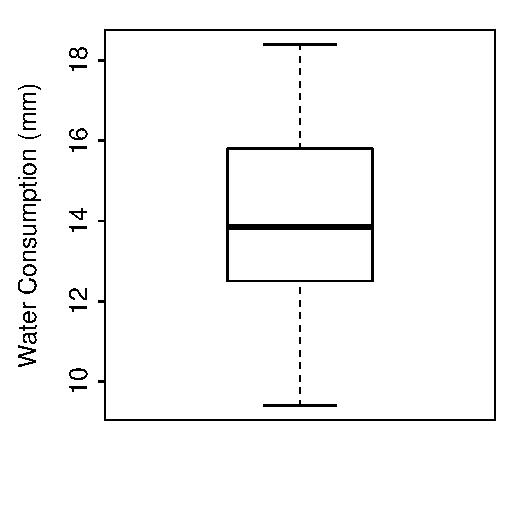
\includegraphics[width=.4\linewidth]{Figs/MouseBoxplot-1} 

}

\caption[Boxplot of the mouse consumption data]{Boxplot of the mouse consumption data.}\label{fig:MouseBoxplot}
\end{figure}


\end{knitrout}

\defn{Boxplot}{Generally, a graphical depiction of the five-number summary.}

The relative length from the median to Q1 and the median to Q3 (i.e., the position of the median line in the box) can give an indication of the shape of a distribution.\index{Boxplot!Interpretation}  If the distribution is left-skewed (i.e., the left tail or lesser-valued individuals is spread out; \figref{fig:BoxplotShape}-Right), then the ``dispersion'' of the individuals in the second quarter of the ordered data (i.e., Q1 - median) will be greater than the ``dispersion'' of the individuals in the third quarter (i.e., median - Q3).  In contrast, if the distribution is right-skewed (i.e., the right tail or larger-valued individuals is spread out; \figref{fig:BoxplotShape}-Middle), then the ``dispersion'' of the individuals in the third quarter of the ordered data will be greater than the ``dispersion'' of the individuals in the second quarter.  Thus, if the distribution is right-skewed, then the median will be closer to Q1 than to Q3.  If the distribution is left-skewed, then the median will be closer to Q3 than to Q1.  If the distribution is approximately symmetric (\figref{fig:BoxplotShape}-Left), then the median will be in the middle of the box (and the middle of the whiskers).

\begin{knitrout}
\definecolor{shadecolor}{rgb}{0.922, 0.922, 0.922}\color{fgcolor}\begin{figure}[hbtp]

{\centering 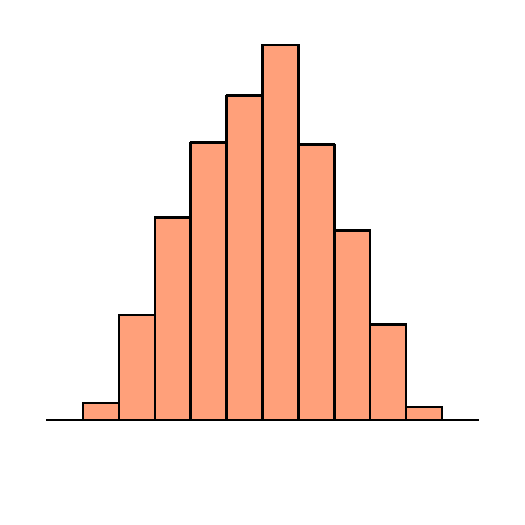
\includegraphics[width=.3\linewidth]{Figs/BoxplotShape-1} 
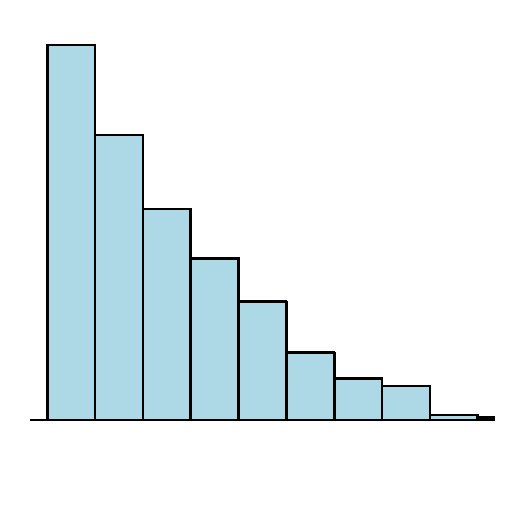
\includegraphics[width=.3\linewidth]{Figs/BoxplotShape-2} 
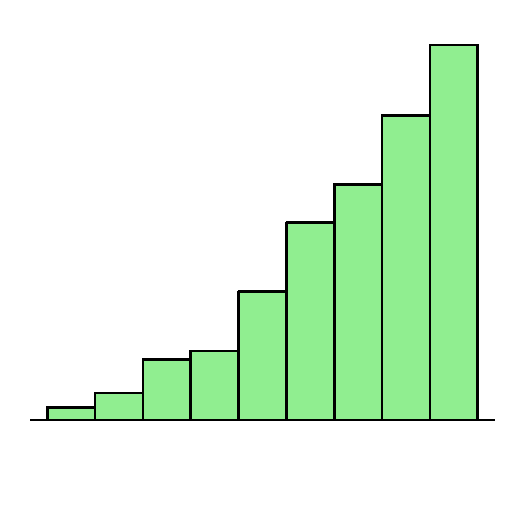
\includegraphics[width=.3\linewidth]{Figs/BoxplotShape-3} 
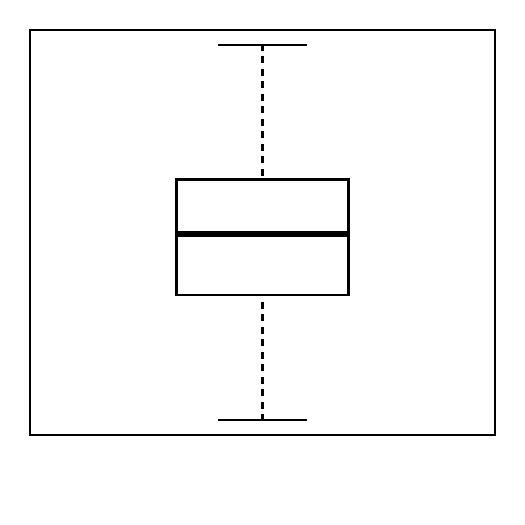
\includegraphics[width=.3\linewidth]{Figs/BoxplotShape-4} 
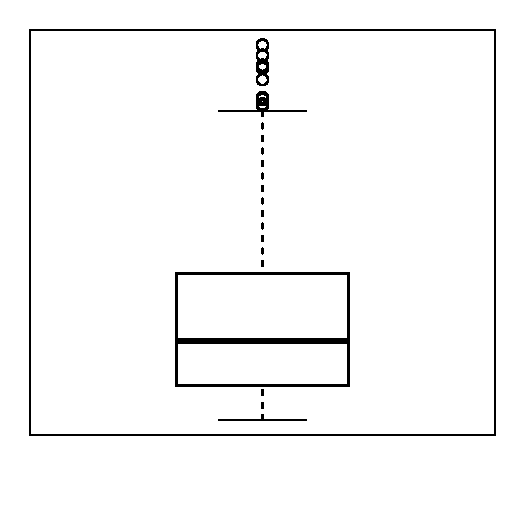
\includegraphics[width=.3\linewidth]{Figs/BoxplotShape-5} 
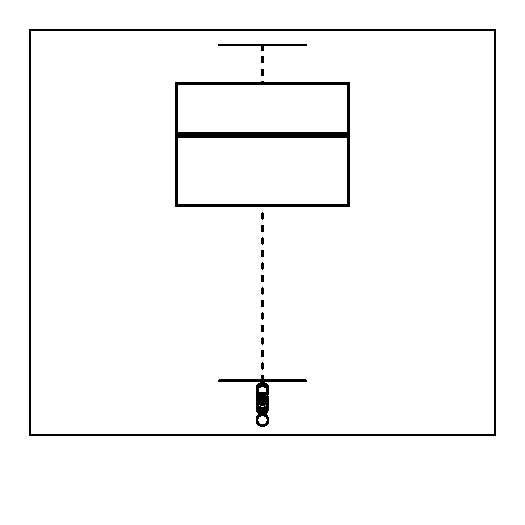
\includegraphics[width=.3\linewidth]{Figs/BoxplotShape-6} 

}

\caption[Histograms and boxplots for several different shapes of distributions]{Histograms and boxplots for several different shapes of distributions.}\label{fig:BoxplotShape}
\end{figure}


\end{knitrout}

\warn{If a distribution is right-skewed, then the median will be closer to Q1 than to Q3. If the distribution is left-skewed, then the median will be closer to Q3 than to Q1.}

\vspace{-12pt}
\warn{Even though shape can be described from a boxplot, it is always easier to describe shape from a histogram.}

A boxplot is constructed in R with \R{boxplot()}.  This function requires only the name of the quantitative variable as the first argument although the x- and y-axes are labeled with \R{xlab=} and \R{ylab=}, respectively.


\begin{exsection}
  \item \label{revex:quEDABrule5N} What is the five-number summary for the maximum gauge heights of the Bois Brule River in Brule, WI from Exercise \ref{revex:quEDABrule}. \ansref{ans:quEDABrule5N}
  \item \label{revex:quEDAWI5N} \rhw{} Construct a boxplot for the population density of Wisconsin counties from Exercise \ref{revex:quEDAWIc}. \ansref{ans:quEDAWI5N}
  \item \label{revex:quEDABoxLeft} What is the shape of the left boxplot below? \ansref{ans:quEDABoxLeft}

\begin{center}
  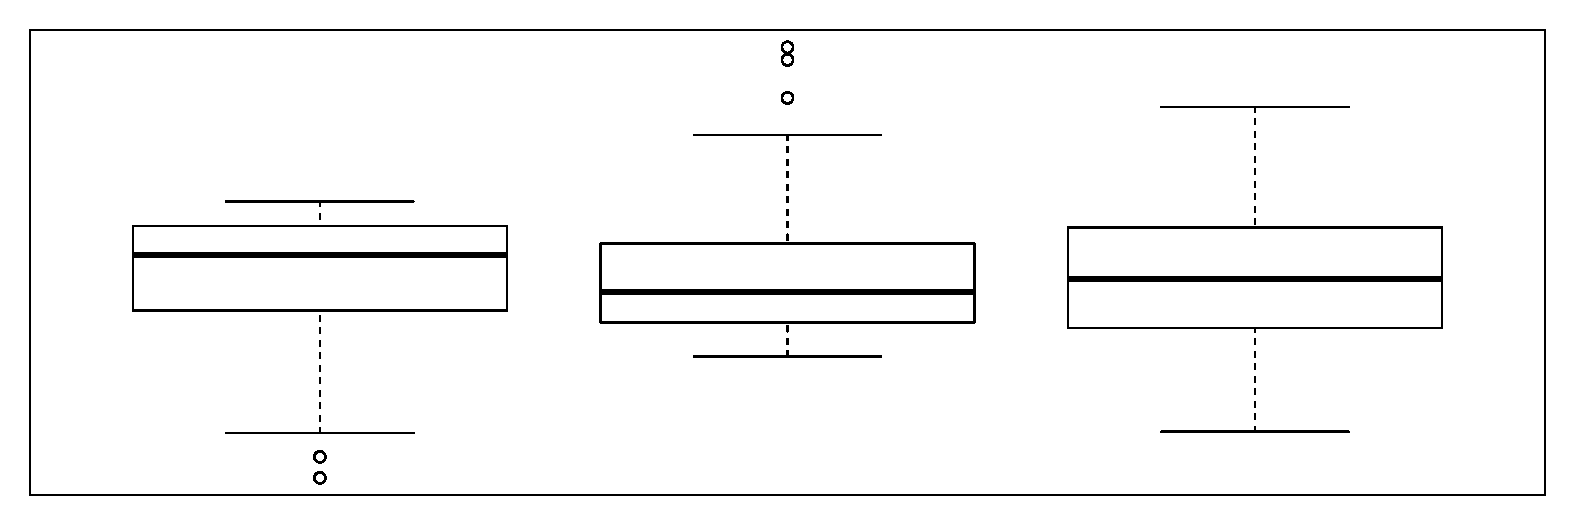
\includegraphics[width=4in]{Figs/BoxplotQuest-1}
\end{center}

  \item \label{revex:quEDABoxRight} What is the shape of the middle boxplot above? \ansref{ans:quEDABoxRight}
  \item \label{revex:quEDABoxSym} What is the shape of the right boxplot above? \ansref{ans:quEDABoxSym}
  \item \label{revex:quEDALSkewCtr} If the distribution is skewed left, which measure should you generally use to measure center? \ansref{ans:quEDALSkewCtr}
  \item \label{revex:quEDARSkewCtr} Which measure of center should you generally use for a right-skewed distribution? \ansref{ans:quEDARSkewCtr}
  \item \label{revex:quEDASymCtr} Which measure of center should you generally use for a symmetric distribution? \ansref{ans:quEDASymCtr}
  \item \label{revex:quEDASymDisp} Which measure of dispersion should you generally use for a symmetric distribution? \ansref{ans:quEDASymDisp}
  \item \label{revex:quEDALSkewDisp} Which measure of dispersion should you generally use for a left-skewed distribution? \ansref{ans:quEDALSkewDisp}
  \item \label{revex:quEDARSkewDisp} Which measure of dispersion should you generally use for a right-skewed distribution? \ansref{ans:quEDARSkewDisp}
  \item \label{revex:quEDAQShape1} Is Q3-Q2 less than, approximately equal to, or greater than Q2-Q1 if the data are left-skewed? \ansref{ans:quEDAQShape1}
  \item \label{revex:quEDAQShape2} What is the shape of the distribution if Q3-Q2 is greater than Q2-Q1? \ansref{ans:quEDAQShape2}
\end{exsection}

\subsection{Multiple Groups} \label{sect:MultGroups}
It is common to conduct a univariate EDA for a quantitative variable separately for multiple groups of individuals.  In these cases it is beneficial to have a function that will efficiently construct a histogram and compute summary statistics for the quantitative variable separated by the levels of a factor variable.  Separate histograms are constructed with \R{hist()} if the first argument is a ``formula'' of the type \R{var\TILDE group} where \R{var} represents the quantitative response variable of interest and \R{group} represents the factor variable that indicates to which group the individual belongs.\index{Histogram!Multiple}  When a formula is supplied as an argument, then the \R{data=} argument becomes required and should be set equal to the data frame containing the variables in the formula.  Summary statistics are separated by group by supplying the same formula and \R{data=} arguments to \R{Summarize()}.

As an example, suppose that you want to examine the average annual days of ice for each decade (using the \R{LSI} data).  One might expect to use the \R{days\TILDE decade} formula except that the \R{decade} variable is not a factor\footnote{It is not a factor because the data in that variable looks numeric to R.}.  A new variable that is a factored version of \var{decade} is created by including \var{decade} into \R{factor()}, as follows,
\begin{knitrout}
\definecolor{shadecolor}{rgb}{0.922, 0.922, 0.922}\color{fgcolor}\begin{kframe}
\begin{verbatim}
> LSI$fdecade <- factor(LSI$decade)
\end{verbatim}
\end{kframe}
\end{knitrout}
Thus, the \R{LSI} data frame now has a new variable, \var{fdecade}, as can be seen with
\begin{knitrout}
\definecolor{shadecolor}{rgb}{0.922, 0.922, 0.922}\color{fgcolor}\begin{kframe}
\begin{verbatim}
> str(LSI)
'data.frame':	42 obs. of  5 variables:
 $ season : int  1955 1956 1957 1958 1959 1960 1961 1962 1963 1964 ...
 $ decade : int  1950 1950 1950 1950 1950 1960 1960 1960 1960 1960 ...
 $ temp   : num  22.9 23 25.7 20 24.8 ...
 $ days   : int  87 137 106 97 105 118 118 136 91 NA ...
 $ fdecade: Factor w/ 5 levels "1950","1960",..: 1 1 1 1 1 2 2 2 2 2 ...
\end{verbatim}
\end{kframe}
\end{knitrout}

Summary statistics and histograms \figrefp{fig:mhist1} separated by decade can then be constructed with

\begin{knitrout}
\definecolor{shadecolor}{rgb}{0.922, 0.922, 0.922}\color{fgcolor}\begin{kframe}
\begin{verbatim}
> Summarize(days~fdecade,data=LSI,digits=2)
  fdecade  n nvalid   mean    sd min     Q1 median    Q3 max percZero
1    1950  5      5 106.40 18.73  87  97.00  105.0 106.0 137        0
2    1960 10      8 113.12 14.80  91 104.20  116.0 119.8 136        0
3    1970 10     10 115.50 19.19  82 105.80  115.0 124.0 146        0
4    1980 10     10 103.80 24.88  48  90.25  116.0 118.0 123        0
5    1990  7      6  96.00 28.53  62  72.00  100.5 114.0 132        0
> hist(days~fdecade,data=LSI,ylab="Days of Ice Cover")
\end{verbatim}
\end{kframe}\begin{figure}[hbtp]

{\centering 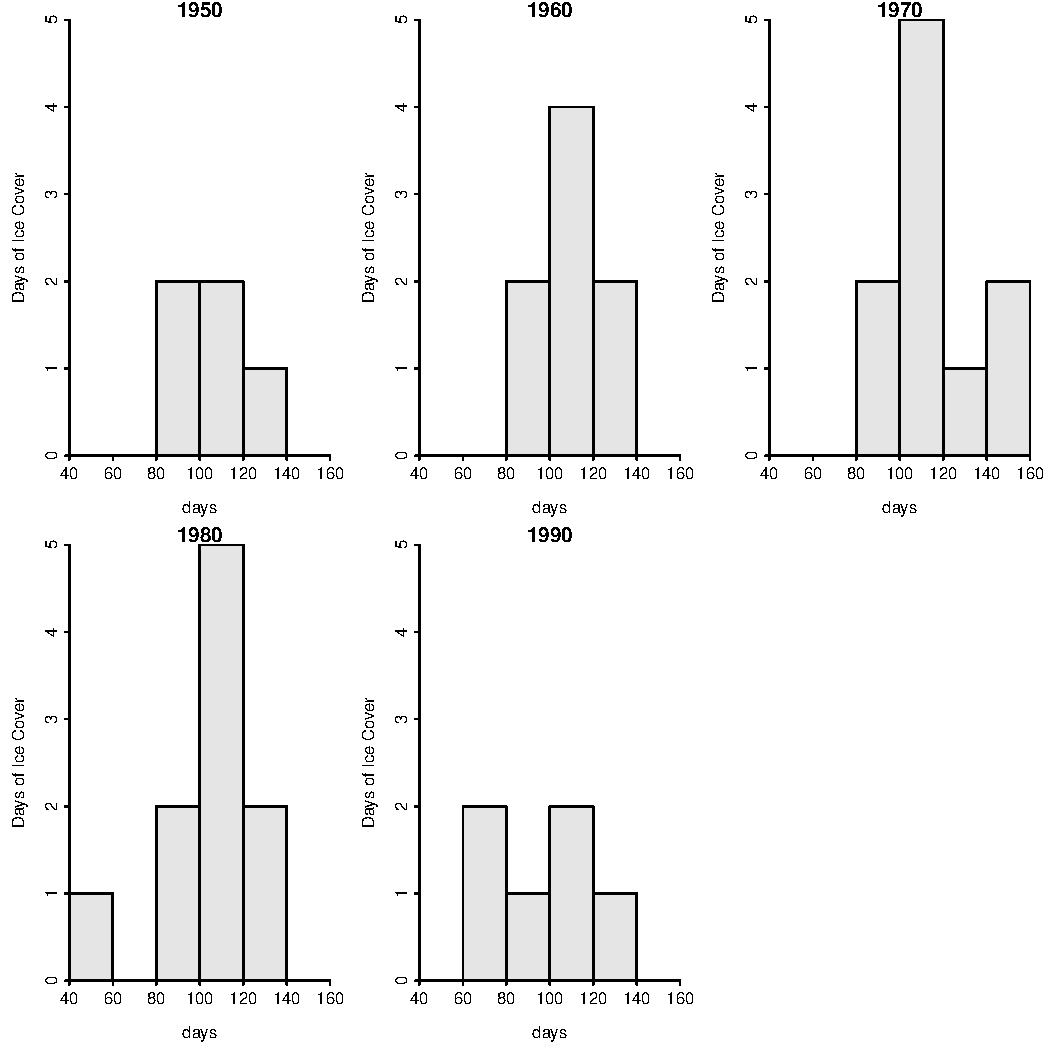
\includegraphics[width=.8\linewidth]{Figs/mhist1-1} 

}

\caption[Histograms of the duration of ice cover at ice gauge 9004 in Lake Superior by each decade]{Histograms of the duration of ice cover at ice gauge 9004 in Lake Superior by each decade.}\label{fig:mhist1}
\end{figure}


\end{knitrout}

The desired grouping variable may already be a factor in some data frames.  It was not in this case because the values in the \R{decade} variable were numerical and will be treated as numbers unless designated by the \R{factor()} function.  Thus, most grouping variables will not require modification by the \R{factor()} function.  Furthermore, note that any variable modification should be stored into a new variable (e.g., \R{fdecade}) so as not to permanently alter (or destroy!) the original data.

Side-by-side boxplots \figrefp{fig:Boxplot1} are an alternative to the separated histograms and are constructed by including the same formula and \R{data=} arguments to \R{boxplot()},

\begin{knitrout}
\definecolor{shadecolor}{rgb}{0.922, 0.922, 0.922}\color{fgcolor}\begin{kframe}
\begin{verbatim}
> boxplot(days~fdecade,data=LSI,ylab="Days of Ice Cover",xlab="Decade")
\end{verbatim}
\end{kframe}\begin{figure}[hbtp]

{\centering 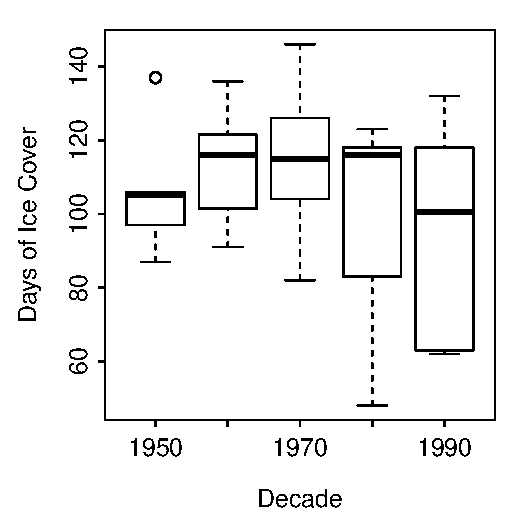
\includegraphics[width=.4\linewidth]{Figs/Boxplot1-1} 

}

\caption[Boxplot of the duration of ice cover at ice gauge 9004 in Lake Superior by each decade]{Boxplot of the duration of ice cover at ice gauge 9004 in Lake Superior by each decade.}\label{fig:Boxplot1}
\end{figure}


\end{knitrout}

\vspace{100pt}
\begin{exsection}
  \item \label{revex:EDAArsenic1} \rhw{} Arsenic concentrations were measured in the well water and in the toe nails of 21 people with home wells.  Also recorded were the person's age, sex, and qualitative measurements of usage for drinking and cooking.  The data are found in \href{https://raw.githubusercontent.com/droglenc/NCData/master/Arsenic.csv}{Arsenic.csv}.  Load these data into R to answer the questions below. \ansref{ans:EDAArsenic1}
  \begin{Enumerate}
    \item Construct a univariate EDA for the well water measurements.
    \item Construct a univariate EDA for the measurements of arsenic in the toe nails.
    \item Construct a univariate EDA for the toe nail arsenic levels separated by levels of drinking water usage.
  \end{Enumerate}
\end{exsection}

\clearpage
\section{Categorical Univariate EDA}  \label{sect:UEDACategorical}
Interpreting summaries of a single categorical variable is more intuitive and less defined than that for quantitative data.\index{EDA!Univariate!Categorical}  Specifically, one DOES NOT describe shape, center, dispersion, and outliers for categorical data.  In this chapter, methods to construct tables and graphs for categorical data will be described and the interpretation of the results will be demonstrated.  These concepts will be illustrated with data recorded on MTH107 students in the Winter 2010 semester.  The sex of a subset of individuals in this data set is shown in \tabref{tab:Mth107SexSubset}.

\begin{table}[htbp]
  \caption{Sex of a subset of individuals in MTH107 in Winter 2010.}
  \label{tab:Mth107SexSubset}
  \centering
  \begin{Verbatim}[xleftmargin=5mm]
Indiv  1  2  3  4  5  6  7  8
Sex    M  F  F  M  M  M  F  M
  \end{Verbatim}
\end{table}


\subsection{Summary Tables}
A simple method to summarize categorical data is to count the number of individuals in each category (or level) of the categorical variable.  These counts are called frequencies and the resulting table \tabrefp{tab:Mth107SexSubsetFreq} is called a frequency table.\index{Table!Frequency}  From this table, it is seen that there were five males and three females in this (subsetted) class.

\begin{table}[htbp]
  \caption{Frequency table of the sex of a subset of individuals in MTH107 in Winter 2010.}
  \label{tab:Mth107SexSubsetFreq}
  \centering
  \begin{Verbatim}[xleftmargin=5mm]
Sex  Freq
 M     5
 F     3
  \end{Verbatim}
\end{table}

\warn{Frequency tables show the total count or number of individuals in each category (or level) of a categorical variable.}

The remainder of this chapter will use the results from the entire class rather than the subset used above to illustrate computing a frequency table.  The frequency tables of individuals by sex and by year-in-school for the entire class is shown in \tabref{tab:Mth107Freq}.

\begin{table}[htbp]
  \caption{Frequency tables of the sex (Left) and year-in-school (Right) of all individuals in MTH107 in Winter 2010.}
  \label{tab:Mth107Freq}
  \centering
  \begin{Verbatim}[xleftmargin=5mm]
Sex  Freq          Year  Freq
 M    38            Fr    19
 F    30            So    12
                    Jr    29
                    Sr     9
   \end{Verbatim}
\end{table}

Many times, frequency tables are modified by showing the percentage, rather than the frequency, of individuals in each category.  These modified tables are called \textbf{percentage tables}.\index{Table!Percentage}  Percentage tables are constructed from frequency tables by dividing the frequency of individuals in each category by the total number of individuals examined ($n$) and then multiplying by 100.  For example, the percentage tables for both sex and year-in-school \tabrefp{tab:Mth107Prop} of students in MTH107 is constructed from \tabref{tab:Mth107Freq} by dividing the value in each cell by 68, the total number of students in the class, and then multiplying by 100.  From this it is seen that 55.9\% of students were male and 13.2\% were seniors.

\begin{table}[htbp]
  \caption{Percentage table of the sex (Left) and year-in-school (Right) of all individuals in MTH107 in Winter 2000.}
  \label{tab:Mth107Prop}
  \centering
  \begin{Verbatim}[xleftmargin=5mm]
Sex   Perc          Year   Perc
 M    55.9           Fr    27.9
 F    44.1           So    17.6
                     Jr    42.6
                     Sr    13.2
  \end{Verbatim}
\end{table}

\warn{Percentage tables show the percentage of all individuals in each category (or level) of a categorical variable.}

\subsection{Tables in R}
The General Sociological Survey (GSS) is a very large survey that has been administered 25 times since 1972.  The basic purpose of the GSS is to gather data on contemporary American society in order to monitor and explain trends in attitudes, behaviors, and attributes.  One question that was asked in a recent GSS was, ``How often do you make a special effort to sort glass or cans or plastic or papers and so on for recycling?''  These data are found in the \var{recycle} variable of the \href{https://raw.githubusercontent.com/droglenc/NCData/master/GSSEnviroQues.csv}{GSSEnviroQues.csv} file.  These data are loaded and observed with
\begin{knitrout}
\definecolor{shadecolor}{rgb}{0.922, 0.922, 0.922}\color{fgcolor}\begin{kframe}
\begin{verbatim}
> GSS <- read.csv("data/GSSEnviroQues.csv")
> str(GSS)
'data.frame':	3539 obs. of  2 variables:
 $ recycle: Factor w/ 5 levels "Always","Never",..: 1 1 1 1 1 1 1 1 1 1 ...
 $ tempgen: Factor w/ 5 levels "Extremely","Not",..: 1 1 1 1 1 1 1 1 1 1 ...
> levels(GSS$recycle)
[1] "Always"    "Never"     "Not Avail" "Often"     "Sometimes"
\end{verbatim}
\end{kframe}
\end{knitrout}

These results show the five levels in the \var{recycle} factor variable.  Note that the levels appear to be out of order because the default for a group factor variable is for the order of the levels to be alphabetical.  The levels should be in the order ``Always'', ``Often'', ``Sometimes'', ``Never'', and ``Not Avail'' to follow the natural order of this ordinal variable.  The order of a factor variable is controlled by including the ordered level names within a vector sent to the \R{levels=} argument in \R{factor()}.\index{Factor!Variable in R}\index{Level!Controlling in R}  The level names in this vector must be exactly as they appear in the original variable and they must be contained within quotes.  The order of the levels of \var{recycle} is changed and stored in a new variable in \var{GSS} with
\begin{knitrout}
\definecolor{shadecolor}{rgb}{0.922, 0.922, 0.922}\color{fgcolor}\begin{kframe}
\begin{verbatim}
> GSS$frecycle <- factor(GSS$recycle,levels=c("Always","Often","Sometimes","Never","Not Avail"))
> levels(GSS$frecycle)
[1] "Always"    "Often"     "Sometimes" "Never"     "Not Avail"
\end{verbatim}
\end{kframe}
\end{knitrout}
The advantage of correcting this order is that when the summary table is made, the order will follow the natural order of the variable rather than the alphabetical order.

\warn{The order of the levels of a factor are controlled with the \R{levels=} argument in the \R{factor()} function.}

\vspace{-12pt}
\warn{When changing the order of the levels with the \R{levels=} argument, the level names must be contained within quotes and they must be spelled exactly as they were spelled in the original variable.}

The frequency table of a single categorical variable is computed with \R{xtabs()} where the first argument is a one-side formula of the form \R{\TILDE var} with the corresponding data.frame in \R{data=}.  The result from \R{xtabs()} should be assigned to an object for further processing.  For example, the frequency table is produced, stored in the \var{tabRecycle} object, and displayed with
\begin{knitrout}
\definecolor{shadecolor}{rgb}{0.922, 0.922, 0.922}\color{fgcolor}\begin{kframe}
\begin{verbatim}
> ( tabRecycle <- xtabs(~frecycle,data=GSS) )
frecycle
   Always     Often Sometimes     Never Not Avail 
     1289       850       823       448       129 
\end{verbatim}
\end{kframe}
\end{knitrout}
Thus, we see that 1289 respondents answered ``Always'' to the recycling question.

The percentage table is computed in R by including the saved frequency table\footnote{Thus, \R{xtabs()} must be completed and saved to an object before \R{percTable()}.} as the first argument to \R{percTable()}.  The number of digits of output is controlled with \R{digits=}  For example, the percentage table is constructed with
\begin{knitrout}
\definecolor{shadecolor}{rgb}{0.922, 0.922, 0.922}\color{fgcolor}\begin{kframe}
\begin{verbatim}
> percTable(tabRecycle)
frecycle
    Always      Often  Sometimes      Never  Not Avail        Sum 
 36.422718  24.018084  23.255157  12.658943   3.645097 100.000000 
\end{verbatim}
\end{kframe}
\end{knitrout}
Thus, we see that 36.4\% of respondents answered ``Always'' to the recycling question.

\subsection{Bar Plots}
Bar plots, or bar charts, are used to display the frequency or percentage of individuals in each category of a categorical variable.\index{Bar Chart}  Bar plots look very similar to histograms as they have frequency of individuals on the y-axis.  However, category labels rather than quantitative values are plotted on the x-axis.  In addition, bars on a bar plot are usually not connected in order to highlight the categorical nature of the data.  A bar plot corresponding to the sex of individuals in MTH107 is shown in \figref{fig:MTH107BarChart}.  This bar plot is not very helpful because there were only two categories (i.e., it does not add much to the frequency table).  However, bar plots make it easier to compare the number of individuals in each category when there are several categories as in \figref{fig:MTH107BarChart}.

\begin{knitrout}
\definecolor{shadecolor}{rgb}{0.922, 0.922, 0.922}\color{fgcolor}\begin{figure}[hbtp]

{\centering 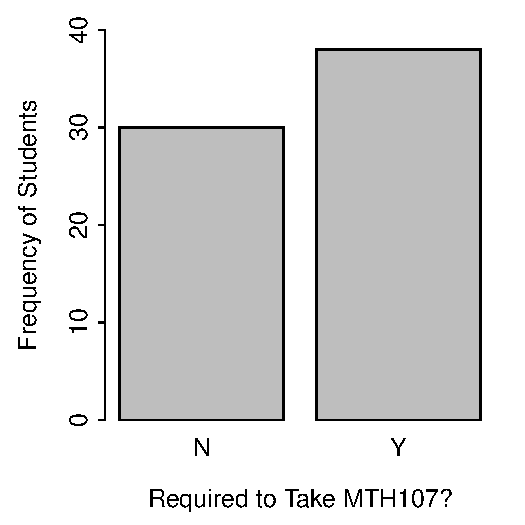
\includegraphics[width=.4\linewidth]{Figs/MTH107BarChart-1} 
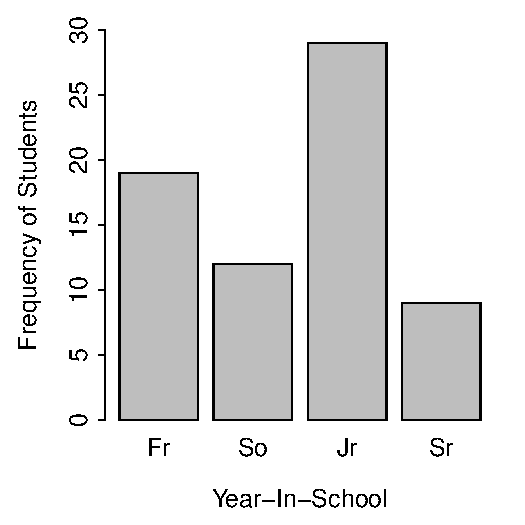
\includegraphics[width=.4\linewidth]{Figs/MTH107BarChart-2} 

}

\caption[Bar charts of the frequency of individuals in MTH107 during Winter 2010 by sex (\textbf{Left}) and year-in-school (\textbf{Right})]{Bar charts of the frequency of individuals in MTH107 during Winter 2010 by sex (\textbf{Left}) and year-in-school (\textbf{Right}).}\label{fig:MTH107BarChart}
\end{figure}


\end{knitrout}

\warn{Bar charts are used to display the frequency of individuals in the categories of a categorical variable. Histograms are used to display the frequency of individuals in classes created from quantitative variables.}

Shape, center, dispersion, and outliers are not described for categorical data because the data is not numerical and, if nominal, no order exists.  In general, the major characteristics of the table or graph are described from an intuitive basis.  For example, there were more males than females in the Winter 2010 MTH107 class and mostly juniors and Freshmen.

\warn{Do not describe shape, center, dispersion, and outliers for a categorical variable.}

\subsubsection{Bar Plots in R} \label{sect:BarChart}\index{Bar Chart!Construction}
A bar plot is produced by submitting the saved table as the first argument to \R{barplot()}.  Again, the x- and y-axis labels should be explicitly defined with the \R{xlab=} and \R{ylab=} arguments, respectively.  The bar plot for the recycling data \figrefp{fig:Barchart1} is produced with

\begin{knitrout}
\definecolor{shadecolor}{rgb}{0.922, 0.922, 0.922}\color{fgcolor}\begin{kframe}
\begin{verbatim}
> barplot(tabRecycle,ylab="Frequency",xlab="Recycle Response")
\end{verbatim}
\end{kframe}\begin{figure}[hbtp]

{\centering 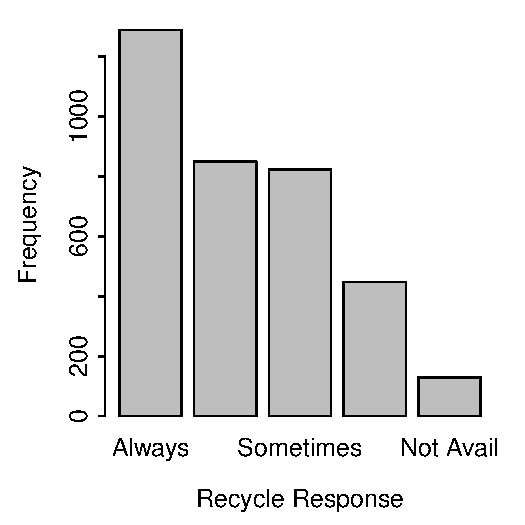
\includegraphics[width=.4\linewidth]{Figs/Barchart1-1} 

}

\caption[Bar chart of the frequency of responses to the recycling question on the GSS]{Bar chart of the frequency of responses to the recycling question on the GSS.}\label{fig:Barchart1}
\end{figure}


\end{knitrout}

\begin{exsection}
  \item \label{revex:EDAArsenic2} \rhw{} Use the \href{https://raw.githubusercontent.com/droglenc/NCData/master/Arsenic.csv}{Arsenic.csv} data in Exercise \ref{revex:EDAArsenic1} to answer the questions below. \ansref{ans:EDAArsenic2}
  \begin{Enumerate}
    \item Construct a univariate EDA for the assessment of drinking water usage.
    \item Construct a univariate EDA for the assessment of cooking water usage.
  \end{Enumerate}

  \item \label{revex:cuEDAEPA}The Environmental Protection Agency (EPA) commissioned the Gallup Organization to conduct a nationwide telephone survey of 1000 households during August and September of 2002 regarding consumer knowledge and satisfaction with drinking water quality.  Of the 1000 respondents surveyed, 751 knew that their drinking water came from a public or commercial water supplier.  Of these 751 respondents, the following percentages knew precisely where that water was derived:

  \begin{center}
  \begin{tabular}{c|c|c|c|c|c}
    \hline\hline
    Ground- & Lake/ &  & Multiple & Don't & Refused \\
    water & Reservoir & River & Sources & Know & Answer \\
    \hline
    15.9\% & 29.2\% & 9.6\% & 15.7\% & 29.4\% & 0.2\% \\
    \hline\hline
  \end{tabular}
  \end{center}

  Use these data to answer the questions below. \ansref{ans:cuEDAEPA}
  \begin{Enumerate}
    \item Construct a frequency table of these data (note percentages above were rounded).
    \item Write a brief conclusion derived from these data.
  \end{Enumerate}

  \item \label{revex:cuEDAHI} \rhw{} A neighborhood in Honolulu conducted a survey to determine if residents participated in the curbside recycling program.  One question on their survey was, ``How much has curbside recycling reduced your regular refuse? 0\%, 25\%, 50\%, 75\%, 100\%, or `too early to tell'?''  The individual responses for the returned surveys are shown below with letters corresponding to the category choices offered (e.g., \verb"A"=0\%, \verb"B"=25\%, and so on).

  \begin{Verbatim}
C, C, B, B, B, B, C, E, B, B, C, B, C, B, C, C, C, E, B, B, B,
C, B, B, C, C, C, B, C, B, C, B, B, C, B, C, B, B, B, C, E, B,
E, B, B, C, C, B, B, B, E, B, C, C, C, B, B, C, B, B, B, B, B
  \end{Verbatim}

  Use these data to answer the questions below. \ansref{ans:cuEDAHI}
  \begin{Enumerate}
    \item Construct a frequency table of these data.
    \item Construct a percentage table of these data.
    \item Write a brief conclusion derived from these data.
  \end{Enumerate}

  \item \label{revex:cuEDARice} \rhw{} Students in a senior level environmental studies class at Rice University conducted a voluntary response survey regarding water usage by their peers.  They received returned surveys from a total 130 students.  One question on their survey was, ``On average, for how many minutes do you let the water run each time you take a shower? 0-5, 6-10, 11-15, or over 15 minutes?''  The individual responses for this survey are shown below with letters corresponding to the category choices offered (e.g., \verb"A"=``0-5'', \verb"B"=``6-10'', and so on). \ansref{ans:cuEDARice}

  \begin{Verbatim}
  D, C, B, B, C, C, B, B, C, C, C, B, D, B, C, C, B, C, D, D,
  B, C, C, A, B, C, C, A, C, C, D, A, C, C, B, B, B, B, B, C,
  D, B, D, B, C, B, C, C, D, C, B, B, D, C, B, C, B, B, C, C,
  B, C, B, C, B, B, C, D, B, C, D, C, B, C, D, C, C, B, C, B,
  D, B, B, D, B, C, B, B, C, B, C, D, D, C, D, B, B, C, B, C,
  A, A, B, C, B, C, D, D, C, B, D, C, C, C, C, A, C, D, B, C,
  B, B, D, C, B, B, A, B, C, B
  \end{Verbatim}

  Use these data to answer the questions below.
  \begin{Enumerate}
    \item Construct a frequency table of these data.
    \item Construct a percentage table of these data.
    \item Write a brief conclusion derived from these data.
  \end{Enumerate}
\end{exsection}


\section{Example Interpretations}\index{EDA!Univariate!Quantitative}
While most of the previous sections focused on how to construct various graphs and numerical summaries, the most important aspect of this chapter is that you can make appropriate interpretations for an EDA from the summary results.  For quantitative data, an appropriate EDA consists of identifying the shape, center, dispersion, and outliers for the variable.  For categorical data, an appropriate EDA consists of identifying the major characteristics among the categories.  Below, I will model properly constructed EDAs for the mouse consumption data and two new data sets.

\subsubsection{Mouse Consumption Example}
\begin{quote}
\textit{Construct a proper EDA for the following situation and data -- `The  following measurements \tabrefp{tab:MouseData} are of the consumption of water in one hour by mice in a laboratory setting.'}
\end{quote}


Mouse water consumption appears to be approximately symmetric without any outliers present \figrefp{fig:MouseHist2}.  The center of the distribution is best measured by the mean, which is 14.05 ml \tabrefp{tab:MouseStats}.  The range of water consumption by the mice in the sample is from 9.4 to 18.4 ml while the dispersion as measured by the standard deviation is 2.41 ml \tabrefp{tab:MouseStats}.  I chose to use the mean and standard deviation because the data were symmetric with no outliers.  [\textit{NOTE: 1) the use of units, 2) the reference to the figure and table, 3) the labeling of the figure and table, 4) I did not present or discuss the median and IQR because I chose to use the mean and standard deviation, 5) I did not use the range alone as a measure of dispersion, 6) I explained why I used the mean and standard deviation rather than the median and IQR, and 7) I provided the R code used.}]

% latex table generated in R 3.3.1 by xtable 1.8-2 package
% Sat Aug 27 14:27:46 2016
\begin{table}[ht]
\centering
\caption{Descriptive statistics of mouse water consumption.} 
\label{tab:MouseStats}
\begin{tabular}{rrrrrrrrrr}
  \hline
n & nvalid & mean & sd & min & Q1 & median & Q3 & max & percZero \\ 
  \hline
30.00 & 30.00 & 14.05 & 2.41 & 9.40 & 12.52 & 13.85 & 15.80 & 18.40 & 0.00 \\ 
   \hline
\end{tabular}
\end{table}


\begin{minipage}{\textwidth}
R commands:
\begin{knitrout}
\definecolor{shadecolor}{rgb}{0.922, 0.922, 0.922}\color{fgcolor}\begin{kframe}
\begin{verbatim}
> setwd("c:/data/")
> mc <- read.csv("MouseData.csv")
> str(mc)
> Summarize(~consump,data=mc,digits=2)
> hist(~consump,data=mc,xlab="Water Consumption (mm)",main="")
\end{verbatim}
\end{kframe}
\end{knitrout}
\end{minipage}

\subsubsection{Crayfish Temperature Selection}
\begin{quote}
\textit{\cite{Peck1985} examined the temperature selection of dominant and subdominant crayfish (\textit{Orconectes virilis}) together in an artificial stream.  The temperature ($^{o}$C) selection by the dominant crayfish in the presence of subdominant crayfish in these experiments was recorded below.  Thoroughly describe all aspects of the distribution of selected temperatures, using appropriate numerical summaries where needed.}
\end{quote}

% latex table generated in R 3.3.1 by xtable 1.8-2 package
% Sat Aug 27 14:27:46 2016
\begin{tabular}{rrrrrrrrrrrrrrrr}
  30 & 26 & 26 & 26 & 25 & 25 & 25 & 25 & 25 & 24 & 24 & 24 & 24 & 24 & 24 & 23 \\ 
  23 & 23 & 23 & 22 & 22 & 22 & 22 & 21 & 21 & 21 & 20 & 20 & 19 & 19 & 18 & 16 \\ 
  \end{tabular}


The shape of the data is slightly left-skewed \figrefp{fig:CrayfishTempHist} with a possible weak outlier at the maximum value of 30$^{o}$C \tabrefp{tab:CrayfishTempStats}.  The center is best measured by the median, which is 23$^{o}$C \tabrefp{tab:CrayfishTempStats} and the dispersion is best measured by the IQR, which is from 21 to 25$^{o}$C \tabrefp{tab:CrayfishTempStats}.

\begin{knitrout}
\definecolor{shadecolor}{rgb}{0.922, 0.922, 0.922}\color{fgcolor}\begin{figure}[hbtp]

{\centering 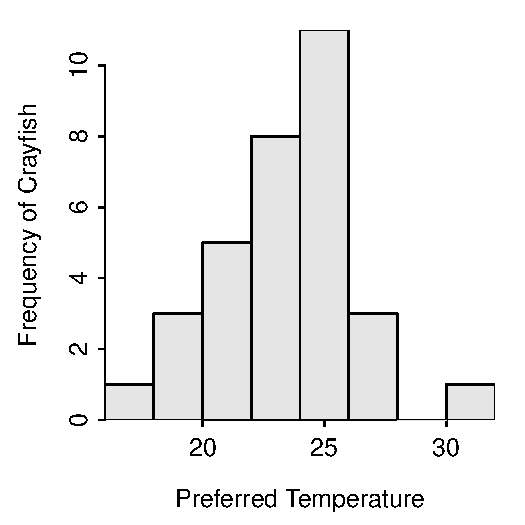
\includegraphics[width=.4\linewidth]{Figs/CrayfishTempHist-1} 

}

\caption[Histogram of crayfish temperature preferences]{Histogram of crayfish temperature preferences.}\label{fig:CrayfishTempHist}
\end{figure}


\end{knitrout}

% latex table generated in R 3.3.1 by xtable 1.8-2 package
% Sat Aug 27 14:27:46 2016
\begin{table}[ht]
\centering
\caption{Descriptive statistics of crayfish temperature preferences.} 
\label{tab:CrayfishTempStats}
\begin{tabular}{rrrrrrrrrr}
  \hline
n & nvalid & mean & sd & min & Q1 & median & Q3 & max & percZero \\ 
  \hline
32.00 & 32.00 & 22.88 & 2.79 & 16.00 & 21.00 & 23.00 & 25.00 & 30.00 & 0.00 \\ 
   \hline
\end{tabular}
\end{table}


\begin{minipage}{\textwidth}
R commands:
\begin{knitrout}
\definecolor{shadecolor}{rgb}{0.922, 0.922, 0.922}\color{fgcolor}\begin{kframe}
\begin{verbatim}
> setwd("c:/data/")
> cray <- read.csv("Crayfish.csv")
> str(cray)
> brks <- seq(15.9,31.9,2)
> hist(~temp,data=cray,breaks=brks,main="",xlab="Preferred Temperature",
 ylab="Frequency of Crayfish")
> Summarize(~temp,data=cray,digits=2)
\end{verbatim}
\end{kframe}
\end{knitrout}
\end{minipage}

\subsubsection{Mixture Seed Count}
\begin{quote}
\textit{A bag of seeds was purchased for seeding a recently constructed wetland.  The purchaser wanted to determine if the percentage of seeds in four broad categories -- ``grasses'', ``sedges'', ``wildflowers'', and ``legumes'' -- was similar to what the seed manufacturer advertised.  The purchaser examined a 0.25-lb sample of seeds from the bag and recorded the results in \href{https://raw.githubusercontent.com/droglenc/NCData/master/WetlandSeeds.csv}{WetlandSeeds.csv}.  Use these data to describe the distribution of seed counts into the four broad categories.}
\end{quote}



The majority of seeds were either sedge or grass with sedge being more than twice as abundant as grass (\tabref{tab:SeedTable}; \figref{fig:SeedBarplot}).  Very few legumes were found in the sample.

\begin{knitrout}
\definecolor{shadecolor}{rgb}{0.922, 0.922, 0.922}\color{fgcolor}\begin{figure}[hbtp]

{\centering 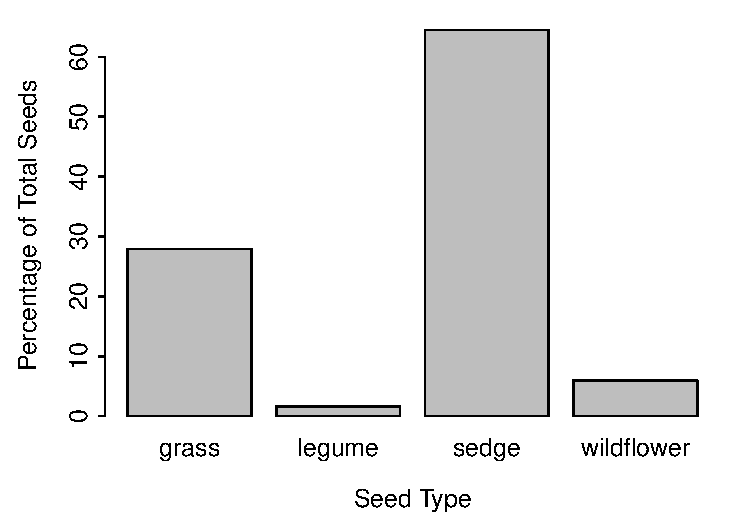
\includegraphics[width=.5\linewidth]{Figs/SeedBarplot-1} 

}

\caption[Barplot of the percentage of wetland seeds by type]{Barplot of the percentage of wetland seeds by type.}\label{fig:SeedBarplot}
\end{figure}


\end{knitrout}

% latex table generated in R 3.3.1 by xtable 1.8-2 package
% Sat Aug 27 14:27:46 2016
\begin{table}[ht]
\centering
\caption{Percentage distribution of wetland seeds by type.} 
\label{tab:SeedTable}
\begin{tabular}{rrrrr}
  \hline
grass & legume & sedge & wildflower & Sum \\ 
  \hline
27.9 & 1.6 & 64.5 & 6.0 & 100.0 \\ 
   \hline
\end{tabular}
\end{table}


\begin{minipage}{\textwidth}
R commands:
\begin{knitrout}
\definecolor{shadecolor}{rgb}{0.922, 0.922, 0.922}\color{fgcolor}\begin{kframe}
\begin{verbatim}
> ws <- read.csv("data/WetlandSeeds.csv")
> str(ws)
> wtbl <- xtabs(~type,data=ws)
> percTable(wtbl,digits=1)
> barplot(wptbl,ylab="Percentage of Total Seeds",xlab="Seed Type")
\end{verbatim}
\end{kframe}
\end{knitrout}
\end{minipage}

\begin{exsection}
  \item \label{revex:quEDAPL} \rhw{} The data below are the number of purple loosestrife (\textit{Lythrum salicaria}) plants found in each of 19 randomly selected plots in the Green Gables Creek Slough.  Describe the distribution of these data.  [\textit{Note: You should use fewer bars on your histogram because the sample size is so small in this situation.}] \ansref{ans:quEDAPL}
    \begin{Verbatim}[xleftmargin=5mm]
13, 2, 1, 0, 9, 11, 5, 5, 14, 23, 0, 2, 3, 3, 6, 7, 4, 16, 1
    \end{Verbatim}
  \item \label{revex:quEDACP} \rhw{} Construct a proper EDA for the creatine phosphokinase data presented in Exercise \ref{revex:quEDACreatPhosph}.  Make sure to defend your choice of numerical summaries.  \ansref{ans:quEDACP}
  \item \label{revex:quEDADJTI} \rhw{} \hspace{12pt} The Dow Jones Travel Index tracks the cost of hotel and car-rental rates in 20 major cities.  For its May 7, 1996, survey the following rates were given for the 20 cities: 152, 180, 167, 119, 115, 113, 119, 135, 140, 126, 114, 133, 205, 104, 149, 124, 127, 161, 106, and 179.  Thoroughly describe the distribution of these data.  [\textit{Note: You can use fewer than the ideal number of bars on your histogram because the sample size is so small in this situation.}] \ansref{ans:quEDADJTI}
  \item \label{revex:cuEDAZoo1} \rhw{} The data in \href{}{Zoo1.csv} contains a list of animals found in several different zoos\footnote{These data are stored in a ``comma separated values'' (CSV) file rather than a ``tab delimited text'' file.  Thus, these data must be loaded into R with \R{read.csv()} rather than \R{read.csv()}.  The arguments to \R{read.csv()} are the same as \R{read.csv()}.}.  In addition, each animal was classified into broad ``type'' categories (``mammal'', ``bird'', and ``amph/rep'').  Perform a univariate EDA on the \var{type} variable. \ansref{ans:cuEDAZoo1}
  \item \label{revex:quEDAZoo2} \rhw{} The data in \href{}{Zoo2.csv} contains the physical size (in acres) of a sample of zoos from around the United States\footnote{These data are stored in a ``comma separated values'' (CSV) file rather than a ``tab delimited text'' file.  Thus, these data must be loaded into R with \R{read.csv()} rather than \R{read.csv()}.  The arguments to \R{read.csv()} are the same as \R{read.csv()}.}.  Perform a univariate EDA on the \var{size} variable. \ansref{ans:quEDAZoo2}
\end{exsection}

\newpage
\begin{hwsection}{All questions below should be typed and answered following the expectations identified in \sectref{sect:ReportWriting}.  All work must be shown.  Questions marked with the R logo must include R output with your R commands in an attached appendix.}

  \item \label{hwprob:quEDABOD} \rhw{} Municipal wastewater treatment plants are required by law to monitor their discharges into rivers and streams on a regular basis.  Concern about the reliability of data from one of these self-monitoring programs led to a study in which samples of effluent were divided and sent to two labs -- a State of Wisconsin lab and a private commercial lab.  Each lab measured the Biological Oxygen Demand (BOD) on the effluent sample sent to them.  Enter these data, in stacked format with two columns labeled \var{lab} and \var{bod} in Excel\footnote{Descriptions for how to enter these data are found in \sectref{sect:REnterData}.}, save the data to a CSV file, and read the data into an object named \var{d} in R.
    \begin{Verbatim}[xleftmargin=5mm]
State -- 6,6,8,11,18,20,28,33,34,43,71
Private -- 15,25,28,29,34,35,36,39,42,44,54
    \end{Verbatim}
  \begin{Enumerate}
    \item List all measurements for the state lab.  [HINT: use \R{filterD()}\footnote{See \sectref{sect:RSubsetdf}.}.]
    \item List the eighth measurement for the state lab.
    \item Perform separate appropriate EDAs for \textbf{each} lab.  Refer to figures and tables as appropriate.  [HINT: construct your figures and tables with one R command each\footnote{See \sectref{sect:MultGroups}.}.]
    \item What major differences did you see in results from the two labs?
  \end{Enumerate}

  \item \label{hwprob:cuEDA} \rhw{} In June 2000, facilities management at the University of Massachusetts -- Boston surveyed lab managers at the University regarding chemical waste disposal.  One question that they asked the survey participants was, ``Which federal agency regulates the disposal of chemical wastes: Occupational Safety and Health Administration, Environmental Protection Agency, Department of Transportation, or National Institutes of Health?''  The individual responses for this survey are shown below by showing the first letter corresponding to each participant's category choice.  Note that one participant did not answer this question and is labeled with a ``U'' for ``unanswered.''  Enter these data into Excel\footnote{A description for how to enter these data is found in \sectref{sect:REnterData}.}, save the data to a CSV file, and load the file into R.  Use these data to answer the questions below.
  \begin{Verbatim}
O, E, E, O, E, E, E, O, D, O, E, O, E, D, E, O, N, O, E, D,
N, E, D, E, D, O, E, O, E, O, E, E, D, O, E, E, E, E, O, E,
N, O, N, O, E, N, E, O, E, E, E, D, N, E, O, E, N, E, E, N,
E, E, E, N, E, E, N, D, D, E, O, O, E, E, E, N, O, O, O, E,
O, O, E, E, U, O, E, O
  \end{Verbatim}

  \begin{Enumerate}
    \item Construct a frequency table of these data.
    \item Construct a percentage table of these data.
    \item Write a brief conclusion regarding the beliefs of lab managers derived from these data.
  \end{Enumerate}
\end{hwsection}



\chapter{Normal Distribution}  \label{chap:NormDist}
\begin{ChapObj}{\boxwidth}
  \textbf{Chapter Objectives:}
  \begin{Enumerate}
    \item Describe what a normal distribution looks like and what parameters control its shape.
    \item Describe simple properties describing the distribution of individuals on a normal distribution.
    \item Compute the proportion of individuals with a particular set of values from a normal distribution (``forward'' calculations).
    \item Compute the range of values for a certain proportion of individuals from a normal distribution (``reverse'' calculations).
  \end{Enumerate}
\end{ChapObj}

\minitoc
\newpage


\lettrine{A}{ model for the distribution} of a single quantitative variable can be visualized by ``fitting'' a smooth curve to a histogram, removing the histogram, and using the remaining curve as a model for the distribution of the entire population of individuals.  This process is illustrated with the set of three figures shown in \figref{fig:NormDensityEx}.  The underlying histogram was computed from the individuals in a very large sample.  The smooth red curve was drawn over the histogram and then removed to serve as a model for the distribution of the entire population.\index{Population Distribution!Normal Distribution}  If the smooth curve follows a known distribution, then certain calculations will be greatly simplified.

\begin{knitrout}
\definecolor{shadecolor}{rgb}{0.922, 0.922, 0.922}\color{fgcolor}\begin{figure}[hbtp]

{\centering 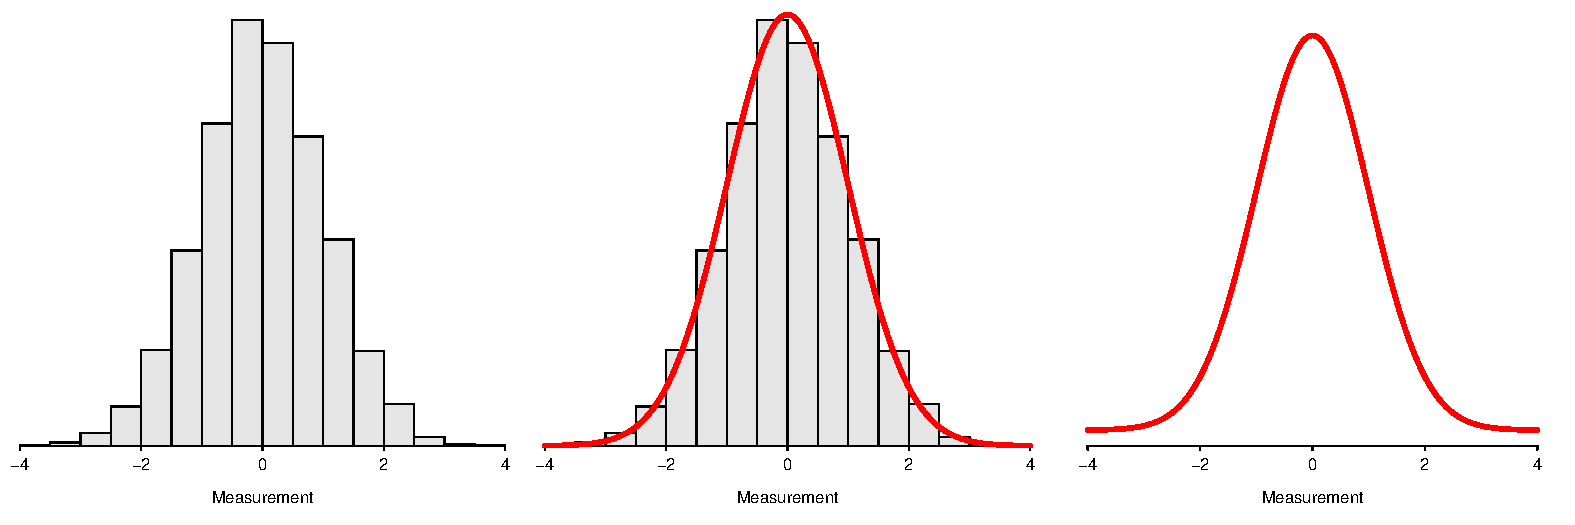
\includegraphics[width=.95\linewidth]{Figs/NormDensityEx-1} 

}

\caption[Depiction of fitting a smooth curve to a histogram and then removing the histogram to leave the smooth curve model]{Depiction of fitting a smooth curve to a histogram and then removing the histogram to leave the smooth curve model.}\label{fig:NormDensityEx}
\end{figure}


\end{knitrout}

The normal distribution is one of the most important distributions in statistics because it serves as a model for the distribution of individuals in many natural situations and the distribution of statistics from repeated samplings (i.e., sampling distributions\footnote{See \chapref{chap:SamplingDist}.}).  The use of a normal distribution model to make certain calculations will be demonstrated in this chapter.

\section{Characteristics}\index{Normal Distribution!Characteristics}
The normal distribution is the common bell-shaped curve that you are probably familiar with (\figref{fig:NormDensityEx}-Right).  Normal distributions are abstractions of reality that are meant to represent all of the individuals in a population.  The height of the curve at a value of $x$ is found with
\begin{equation}
  \label{eqn:NormDistfx}
    f(x) = \frac{1}{\sigma\sqrt{2\pi}}e^{-\frac{1}{2}\left(\frac{x-\mu}{\sigma}\right)^{2}}
\end{equation}
which has the two parameters\footnote{The $e$ and $\pi$ are the usual numerical constants.} -- the population mean, $\mu$,\index{Mean!Population symbol} and the population standard deviation, $\sigma$.\index{Standard Deviation!Population symbol}  The mean, $\mu$, controls the center and the standard deviation, $\sigma$, controls the dispersion of the normal distribution \figrefp{fig:NormMultDists}.

\begin{knitrout}
\definecolor{shadecolor}{rgb}{0.922, 0.922, 0.922}\color{fgcolor}\begin{figure}[hbtp]

{\centering 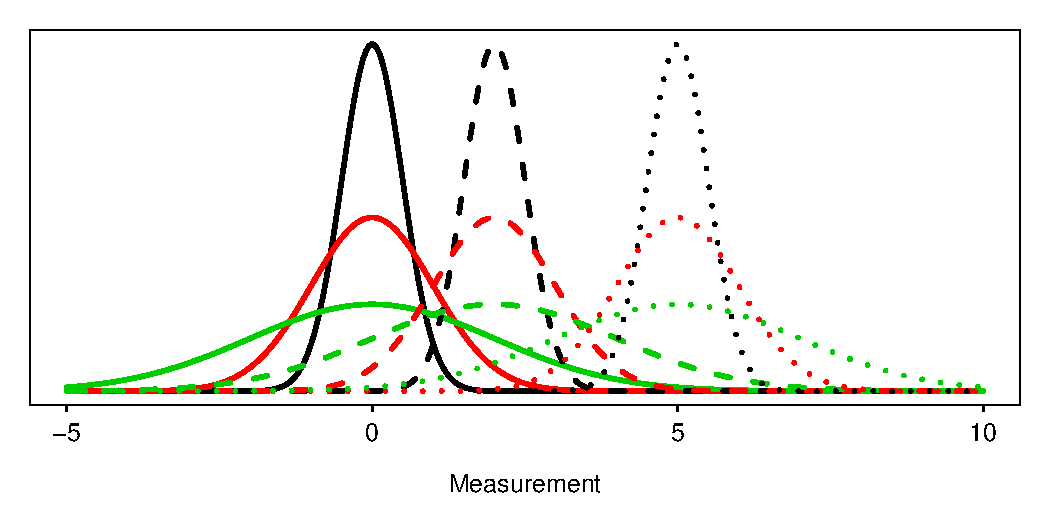
\includegraphics[width=.8\linewidth]{Figs/NormMultDists-1} 

}

\caption[Multiple normal distributions]{Multiple normal distributions.  Distributions with the same line type have the same value of $\mu$.  Distributions with the same color have the same value of $\sigma$.  Values of $\mu$ are 0 (solid), 2 (dashed), and 5 (dotted).  Values of $\sigma$ are 0.5 (black), 1 (red), and 2 (green).}\label{fig:NormMultDists}
\end{figure}


\end{knitrout}

\warn{It is not important that you remember the equation for the height of a normal distribution; you need to remember, though, that the exact position and width of the normal distribution is controlled \textsc{\textbf{only}} by the values of $\mu$ and $\sigma$.}

\begin{minipage}{\textwidth}
There are an infinite number of normal distributions because there are an infinite number of combinations of $\mu$ and $\sigma$.  However, each normal distribution will
\begin{Enumerate}
  \item be bell-shaped and symmetric,
  \item have a center at $\mu$,
  \item have inflection points at $\mu \pm \sigma$, and
  \item have a total area under the curve equal to 1.
\end{Enumerate}
\end{minipage}

\warn{All normal distributions are bell-shaped. The center and dispersion of each, though, is dictated by the values of $\mu$ and $\sigma$, respectively.}

If a generic variable $X$ follows a normal distribution with a mean of $\mu$ and a standard deviation of $\sigma$, then it is said that $X\sim N(\mu,\sigma)$.\index{Normal Distribution!Symbol}  For example, if the heights of students ($H$) follows a normal distribution with a $\mu$ of 66 and a $\sigma$ of 3, then it is said that $H\sim N(66,3)$.  As another example, $Z\sim N(0,1)$ means that the variable $Z$ follows a normal distribution with a mean of $\mu$=0 and a standard deviation of $\sigma$=1.

\warn{A generic variable $X$ that is normally distributed with a mean of $\mu$ and standard deviation of $\sigma$ is abbreviated as $X\sim N(\mu,\sigma)$.}


\section{Simple Areas Under the Curve}
A common statistical problem is to determine the proportion of individuals that have values of the variable between two numbers.  For example, you might be faced with determining the proportion of all sites that have lead concentrations between 1.2 and 1.5 $\mu g \bullet m^{-3}$, the proportion of students that scored higher that 700 on the SAT, or the proportion of least weasels that are shorter than 150 mm.  Before considering these more realistic situations we will explore the calculations for the generic variable $X$ shown in \figref{fig:NormDistShade}.

Let's consider finding the proportion of individuals in a \textit{sample} with values between 0 and 2.  A histogram can be used to answer this question because it is about the individuals in a sample (\figref{fig:NormDistShade}-Left).  In this case, the proportion of individuals with values between 0 and 2 is computed by dividing the number of individuals in the red shaded bars by the total number of individuals in the histogram.  The analogous computation on the superimposed smooth curve is to find the area under the curve between 0 and 2 (\figref{fig:NormDistShade}-Right).  The area under the curve is a ``proportion of the total'' because, as stated above, the area under the entire curve is equal to 1.  The actual calculations on the normal curve will be shown in the following sections.  However, at this point, note that the calculation of an area on a normal curve is analogous to summing the number of individuals in the appropriate classes of the histogram and dividing by $n$.

\begin{knitrout}
\definecolor{shadecolor}{rgb}{0.922, 0.922, 0.922}\color{fgcolor}\begin{figure}[hbtp]

{\centering 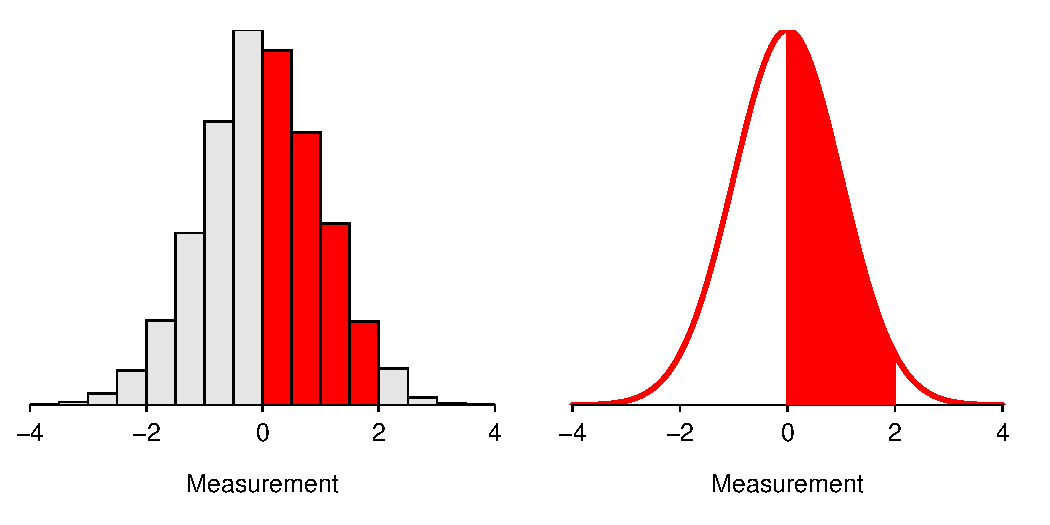
\includegraphics[width=.8\linewidth]{Figs/NormDistShade-1} 

}

\caption[Depiction of finding the proportion of individuals between 0 and 2 on a histogram (\textbf{Left}) and on a standard normal distribution (\textbf{Right})]{Depiction of finding the proportion of individuals between 0 and 2 on a histogram (\textbf{Left}) and on a standard normal distribution (\textbf{Right}).}\label{fig:NormDistShade}
\end{figure}


\end{knitrout}

\warn{The proportion of individuals between two values of a variable that is normally distributed is found by finding the area under the normal distribution between those two values.}

The 68-95-99.7 Rule\footnote{Other authors call this the ``Empirical Rule.''} states that 68\% of the individuals that follow a normal distribution will have values between $\mu-1\sigma$ and $\mu+1\sigma$, 95\% will be between $\mu-2\sigma$ and $\mu+2\sigma$, and 99.7\% will be between $\mu-3\sigma$ and $\mu+3\sigma$ \figrefp{fig:NormEmpiricalRule}.\index{Normal Distribution!68-95-99.7\% Rule}\index{68-95-99.7\% Rule}  The 68-95-99.7 Rule is true no matter what $\mu$ and $\sigma$ are as long as the distribution is normal.  For example, if $A\sim N(3,1)$, then 68\% of the individuals will fall between 2 (i.e., 3-1*1) and 4 (i.e., 3+1*1) and 99.7\% will fall between 0 (i.e., 3-3*1) and 6 (i.e., 3+3*1).  Alternatively, if $B\sim N(9,3)$, then 68\% of the individuals will fall between 6 (i.e., 9-1*3) and 12 (i.e., 9+1*3) and 95\% will be between 3 (i.e., 9-2*3) and 15 (i.e., 9+2*3).  Similar calculations can be made for any normal distribution.

\begin{knitrout}
\definecolor{shadecolor}{rgb}{0.922, 0.922, 0.922}\color{fgcolor}\begin{figure}[hbtp]

{\centering 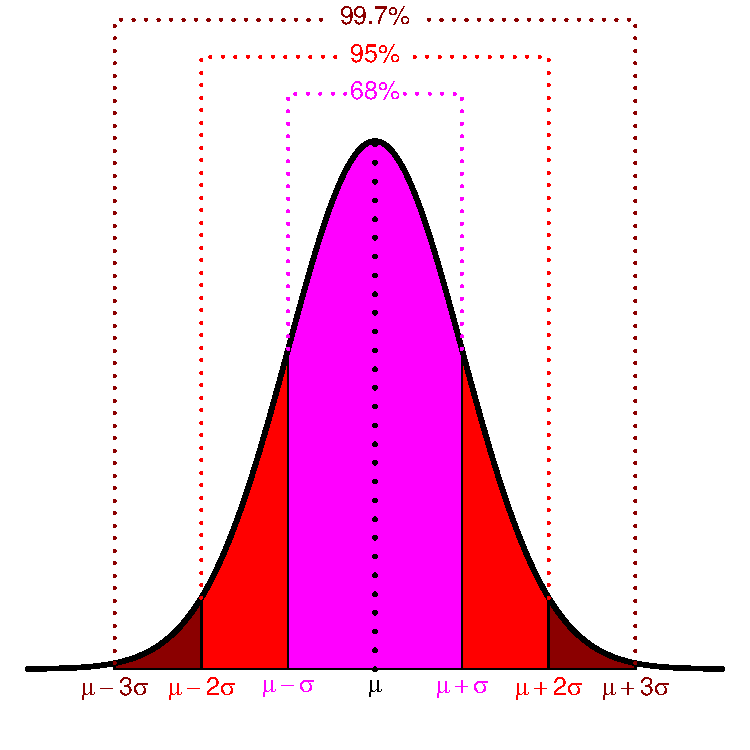
\includegraphics[width=.5\linewidth]{Figs/NormEmpiricalRule-1} 

}

\caption[Depiction of the 68-95-99.7 (or Empirical) Rule on a normal distribution]{Depiction of the 68-95-99.7 (or Empirical) Rule on a normal distribution.}\label{fig:NormEmpiricalRule}
\end{figure}


\end{knitrout}

\defn{68-95-99.7 Rule}{For all normal distributions 68\% of the individuals will be between $\mu\pm1\sigma$, 95\% will be between $\mu\pm2\sigma$, and 99.7\% will be between $\mu\pm3\sigma$}

The 68-95-99.7 Rule is used to find areas under the normal curve as long as the value of interest is an \textbf{integer} number of standard deviations away from the mean.  For example, the proportion of individuals that have a value of A greater than 5 is found by first realizing that 95\% of the individuals on this distribution fall between 1 and 5.  By subtraction this means that 5\% of the individuals must be less than 1 \textbf{AND} greater than 5.  Finally, because of the symmetry of normal distributions, the same proportion of individuals must be less than 1 as are greater than 5.  Thus, half of 5\%, or 2.5\%, of the individuals have a value of A greater than 5.

\warn{The 68-95-99.7 Rule can only be used for questions involving \textbf{integer} standard deviations away from the mean.}

\begin{exsection}
  \item \label{revex:quNorm68} On any normal distribution, what percentage of the individuals is within $\pm1\sigma$ of $\mu$? \ansref{ans:quNorm68}
  \item \label{revex:quNorm68gt} On any normal distribution, what percentage of the individuals are greater than $\mu+\sigma$? \ansref{ans:quNorm68gt}
  \item \label{revex:quNorm95gt} On any normal distribution, what percentage of the individuals are greater than $\mu-2\sigma$? \ansref{ans:quNorm95gt}
  \item \label{revex:quNormbt6895} On any normal distribution, what percentage of the individuals are between $\mu-2\sigma$ and $\mu+1\sigma$? \ansref{ans:quNormbt6895}
  \item \label{revex:quNorm84} On a N(-1,1) distribution, what percentage of the individuals are negative? \ansref{ans:quNorm84}
  \item \label{revex:quNorm16} On a N(100,20) distribution, what percentage of the individuals are less than 80? \ansref{ans:quNorm16}
  \item \label{revex:quNorm16a} On a N(-20,100) distribution, what percentage of the individuals are greater than 80? \ansref{ans:quNorm16a}
  \item \label{revex:quNormAB} Identify the mean and standard deviation for each population on the graph below (HINT: ``eyeball'' integers). \ansref{ans:quNormAB}

    \begin{center}
      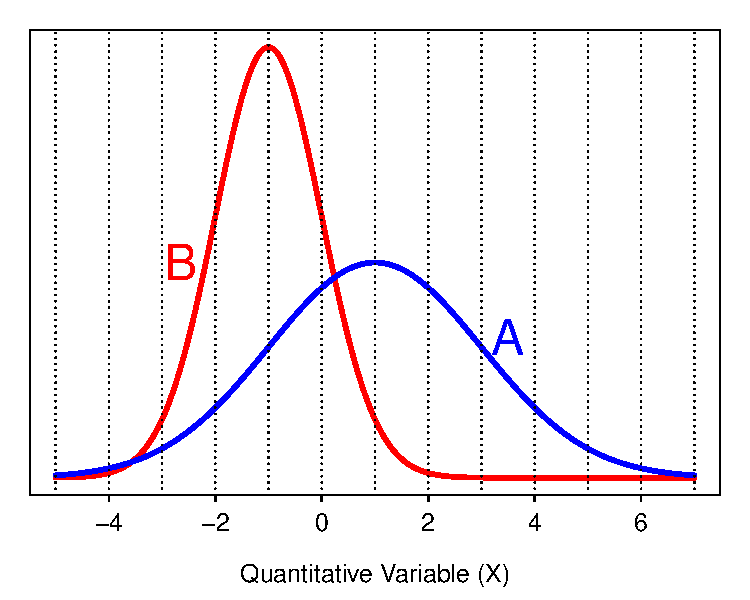
\includegraphics[width=3in]{Figs/Guess-1}
    \end{center}
\end{exsection}


\section[Forward Calculations]{More Complex Areas (Forward Calculations)}
Areas under the curve relative to a non-integer number of standard deviations away from the mean used to be found via a calculation and examination of a so-called standard normal table.  With the advent of computers and cheap software these areas are now found simply with the aid of computer software like R.  The area under a normal curve relative to a particular value is computed in R with \R{distrib()}.  This function requires the \textit{particular value} as the first argument, the mean of the normal distribution in the \R{mean=} argument, and the standard deviation of the normal distribution in the \R{sd=} argument.  The \R{distrib()} function defaults to finding the area under the curve to the \textbf{left of} the particular value but it can find the area under the curve to the right of the particular value by including the \R{lower.tail=FALSE} argument.

For example, suppose that the heights of a population of students, represented by $H$, is known to be $H\sim N(66,3)$.  Thus, the proportion of students in this population that have a height less than 71 inches is computed with (the results are shown below and in \figref{fig:NormZCalc1}),
\begin{knitrout}
\definecolor{shadecolor}{rgb}{0.922, 0.922, 0.922}\color{fgcolor}\begin{kframe}
\begin{verbatim}
> ( distrib(71,mean=66,sd=3) )
[1] 0.9522096
\end{verbatim}
\end{kframe}\begin{figure}[hbtp]

{\centering 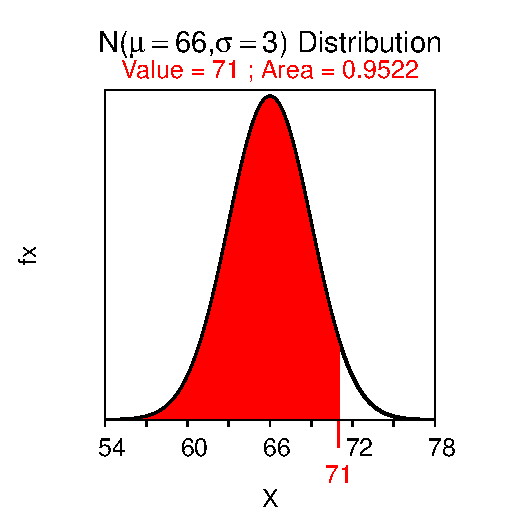
\includegraphics[width=.4\linewidth]{Figs/NormZCalc1-1} 

}

\caption[Calculation of the proportion of individuals on a $N(66,3)$ with a value less than 71]{Calculation of the proportion of individuals on a $N(66,3)$ with a value less than 71.}\label{fig:NormZCalc1}
\end{figure}


\end{knitrout}
Thus, approximately 95.2\% of the students in this population have a height less than 71 inches.  The proportion of students in this population that have a height \textit{greater} than 68 inches is computed by including the \R{lower.tail=FALSE} argument as follows (with the results shown below and in \figref{fig:NormZCalc2}),
\begin{knitrout}
\definecolor{shadecolor}{rgb}{0.922, 0.922, 0.922}\color{fgcolor}\begin{kframe}
\begin{verbatim}
> ( distrib(68,mean=66,sd=3,lower.tail=FALSE) )
[1] 0.2524925
\end{verbatim}
\end{kframe}\begin{figure}[hbtp]

{\centering 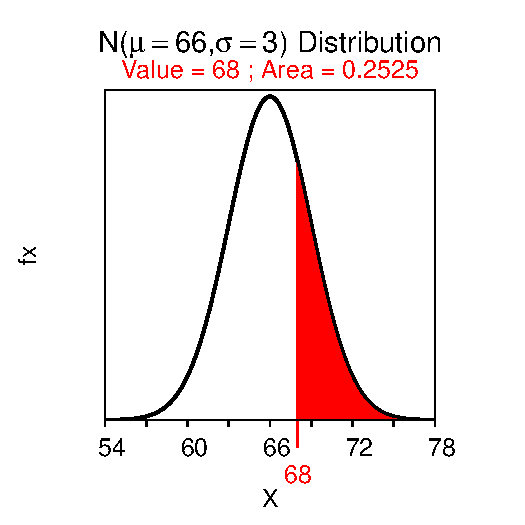
\includegraphics[width=.4\linewidth]{Figs/NormZCalc2-1} 

}

\caption[Calculation of the proportion of individuals on a $N(66,3)$ with a value greater than 68]{Calculation of the proportion of individuals on a $N(66,3)$ with a value greater than 68.}\label{fig:NormZCalc2}
\end{figure}


\end{knitrout}
Thus, approximately 25.2\% of the students in this population have a height greater than 68 inches.

\warn{The area greater than a particular value is found by including the \R{lower.tail=FALSE} argument in \R{distrib()}.}

Finding the area between two particular values is a bit more work.  To answer ``between''-type problems, the area less than the smaller of the two values is subtracted from the area less than the larger of the two values.  This is illustrated by noting that two values split the area under the normal curve into three parts -- A, B, and C \figrefp{fig:NormDistBetween}.  The area between the two values is B.  The area to the left of the larger value corresponds to the combined area of A and B (i.e., A+B).  The area to the left of the smaller value corresponds to the area A.  Thus, subtracting the latter from the former leaves the ``in-between'' area B (i.e., (A+B)-A = B).

\begin{knitrout}
\definecolor{shadecolor}{rgb}{0.922, 0.922, 0.922}\color{fgcolor}\begin{figure}[hbtp]

{\centering \includegraphics[width=.4\linewidth]{Figs/NormDistBetween-1} 

}

\caption[Schematic representation of how to find the area between two $Z$ values]{Schematic representation of how to find the area between two $Z$ values.}\label{fig:NormDistBetween}
\end{figure}


\end{knitrout}

For example, the area between 62 and 70 inches of height is found with (with intermediate calculations shown in \figref{fig:NormZCalc3})

\begin{knitrout}
\definecolor{shadecolor}{rgb}{0.922, 0.922, 0.922}\color{fgcolor}\begin{kframe}
\begin{verbatim}
[1] 0.9087888
> ( A <- distrib(62,mean=66,sd=3) )
[1] 0.09121122
> AB-A
[1] 0.8175776
\end{verbatim}
\end{kframe}\begin{figure}[hbtp]

{\centering \includegraphics[width=.4\linewidth]{Figs/NormZCalc3-1} 
\includegraphics[width=.4\linewidth]{Figs/NormZCalc3-2} 

}

\caption[Calculation of the areas less than 70 inches (\textbf{Left}) and 62 inches (	extbf{Right})]{Calculation of the areas less than 70 inches (\textbf{Left}) and 62 inches (	extbf{Right}).}\label{fig:NormZCalc3}
\end{figure}


\end{knitrout}

Thus, 81.8\% of students in this population have a height between 62 and 70 inches.

\warn{The area between two values is found by subtracting the area less than the smaller value from the area less than the larger value.}

\begin{exsection}
  \item \label{revex:quNormZ0.11} If $X\sim N(0,1)$, then what is the percentage of $X<0.11$? \ansref{ans:quNormZ0.11}
  \item \label{revex:quNormZm0.11} If $X\sim N(0,1)$, then what is the percentage of $X>-0.11$? \ansref{ans:quNormZm0.11}
  \item \label{revex:quNormZbtwn} If $X\sim N(0,1)$, then what is the percentage of $-1.45<X<1.11$? \ansref{ans:quNormZbtwn}
  \item \label{revex:quNormXgt75} If $Y\sim N(70,6)$, then what is the percentage of $Y>75$? \ansref{ans:quNormXgt75}
  \item \label{revex:quNormXlt63} If $Y\sim N(70,6)$, then what is the percentage of $Y<63$? \ansref{ans:quNormXlt63}
  \item \label{revex:quNormXbtwn} If $Y\sim N(70,6)$, then what is the percentage of $62.3<Y<72.9$? \ansref{ans:quNormXbtwn}
\end{exsection}


\section[Reverse Calculations]{Values from Areas (Reverse Calculations)}
Another important calculation with normal distributions is finding the value or values of $X$ with a given proportion of individuals less than, greater than, or between.  For example, it may be necessary to find the test score such that 90\% (or 0.90 as a proportion) of the students scored lower.  In contrast to the calculations in the previous section, the value of $X$ is given and a proportion of individuals (or area) is asked for, the calculations in this section give a proportion and ask for a value of $X$.  These types of questions have been dubbed \textbf{``reverse'' normal distribution questions} to contrast them with the questions in the previous section.

Reverse questions are also answered with \R{distrib()}.  Again, the first argument must be the value of interest -- a proportion (or area) in these questions -- and the mean and standard deviation are given in \R{mean=} and \R{sd=}, respectively.  However, the question is treated as a ``reverse'' question when the \R{type="q"} argument\footnote{``q'' stands for quantile.} is supplied.  Thus, the height that has 20\% of all individuals shorter \figrefp{fig:NormZCalc4} is computed with
\begin{knitrout}
\definecolor{shadecolor}{rgb}{0.922, 0.922, 0.922}\color{fgcolor}\begin{kframe}
\begin{verbatim}
> ( distrib(0.20,mean=66,sd=3,type="q") )
[1] 63.47514
\end{verbatim}
\end{kframe}\begin{figure}[hbtp]

{\centering \includegraphics[width=.4\linewidth]{Figs/NormZCalc4-1} 

}

\caption[Calculation of the height with 20\% of all students shorter]{Calculation of the height with 20\% of all students shorter.}\label{fig:NormZCalc4}
\end{figure}


\end{knitrout}

Thus, 20\% of the population of students is shorter than 63.5 inches.  ``Greater than'' reverse questions are computed by including the \R{lower.tail=FALSE} argument.  For example, the top 10\% of heights \figrefp{fig:NormZCalc5} is found with
\begin{knitrout}
\definecolor{shadecolor}{rgb}{0.922, 0.922, 0.922}\color{fgcolor}\begin{kframe}
\begin{verbatim}
> ( distrib(0.10,mean=66,sd=3,type="q",lower.tail=FALSE) )
[1] 69.84465
\end{verbatim}
\end{kframe}\begin{figure}[hbtp]

{\centering \includegraphics[width=.4\linewidth]{Figs/NormZCalc5-1} 

}

\caption[Calculation of the height with 10\% of all students taller]{Calculation of the height with 10\% of all students taller.}\label{fig:NormZCalc5}
\end{figure}


\end{knitrout}

Thus, 10\% of the population of students is taller than 69.8 inches.

``Between'' questions can only be easily handled if the question is looking for endpoint values that are symmetric about $\mu$.  In other words, the question must ask for the two values that contain the ``most common'' proportion of individuals.  For example, suppose that you were asked to find the most common 80\% of heights.  This type of question is handled by converting this ``symmetric between'' question into two ``less than'' questions.  For example, in \figref{fig:NormRevBetween} the area D is the symmetric area of interest.  If D is 0.80, then C+E must be 0.20\footnote{Because all three areas must sum to 1.}.  Because D is symmetric about $mu$, C and E must both equal 0.10.  Thus, the lower bound on D is the value that has 10\% of all values smaller.  Similarly, because the combined area of C and D is 0.90, the upper bound on D is the value that has 90\% of all values smaller.  This question has now been converted from a ``symmetric between'' to two ``less than'' questions that can be answered exactly as shown above.  For example, the two heights that have a symmetric 80\% of individuals between them are 62.2 and 69.8 as computed with
\begin{knitrout}
\definecolor{shadecolor}{rgb}{0.922, 0.922, 0.922}\color{fgcolor}\begin{kframe}
\begin{verbatim}
> ( distrib(0.10,mean=66,sd=3,type="q") )
[1] 62.15535
> ( distrib(0.90,mean=66,sd=3,type="q") )
[1] 69.84465
\end{verbatim}
\end{kframe}
\end{knitrout}

\begin{knitrout}
\definecolor{shadecolor}{rgb}{0.922, 0.922, 0.922}\color{fgcolor}\begin{figure}[hbtp]

{\centering \includegraphics[width=.4\linewidth]{Figs/NormRevBetween-1} 

}

\caption[Depiction of areas in a reverse between type normal distribution question]{Depiction of areas in a reverse between type normal distribution question.}\label{fig:NormRevBetween}
\end{figure}


\end{knitrout}

\begin{exsection}
  \item \label{revex:quNormXrev03} If $Y\sim N(70,6)$, then what is Y such that the area to the left of it is 0.3? \ansref{ans:quNormXrev03}
  \item \label{revex:quNormXrev04} If $Y\sim N(70,6)$, then what is Y such that the area to the right of it is 0.4? \ansref{ans:quNormXrev04}
  \item \label{revex:quNormXrev05} If $Y\sim N(70,6)$, then what are the Ys such that the area between them is 0.5? \ansref{ans:quNormXrev05}
\end{exsection}


\subsection{Distinguish Calculation Types}\index{Normal Distribution!Finding areas}\index{Normal Distribution!Finding values}
It is critical to be able to distinguish between the two main types of calculations made with normal distributions.  The first type of calculation is a ``forward'' calculation where the area or proportion of individuals relative to a value of the variable must be found.  The second type of calculation is a ``reverse'' calculation where the value of the variable relative to a particular area is calculated.

Distinguishing between these two types of calculations a matter of deciding if (i) the value of the variable is known and the proportion (or area) is to be found or (ii) if the proportion (or area) is known and the value of the variable is to be found.  Therefore, distinguishing between the calculation types is as simple as identifying what is known and what must be found.  If the value of the variable is known but not the proportion or area, then a forward calculation is used.  If the area or proportion is known, then a reverse calculation to find the value of the variable is used.

\begin{exsection}
  \item \label{revex:quNormStudentAge} The age at which ``traditional'' students graduate from college is N(22.1, 1.1).  Use this information to answer the questions below. \ansref{ans:quNormStudentAge}
\begin{Enumerate}
  \item What percentage of the students graduate by the age of 21?
  \item What percentage of the students graduate after age 24?
  \item What is the age range for the middle 95\% of the students?
  \item What is the age at which 90\% of the students have graduated?
\end{Enumerate}

  \item \label{revex:quNormBlackBears} We know, from years of study of black bears, that the population distributions for head length is N(13.7,1.9), neck girth is N(20.9,4.8), and body length is N(60.0,10). All other variables measured on black bears cannot be described by a normal distribution.  Use this information to answer the questions below. \ansref{ans:quNormBlackBears}
\begin{Enumerate}
  \item What is the percentage of bears between 45" and 65" in body length?
  \item What is the percentage of bears that weighs more than 200 lbs?
\end{Enumerate}

  \item \label{revex:quNormShrews} The brain weights of short-tailed shrews (\textit{Blarina brevicauda}) is normally distributed with a mean of 0.14 grams and a standard deviation of 0.04 grams. Use this information to answer the questions below. \ansref{ans:quNormShrews}
\begin{Enumerate}
  \item What percentage of shrews have a brain weight less than 0.09 grams?
  \item What percentage of shrews have a brain weight between 0.09 and 0.17 grams?
  \item What is the brain weight such that 30\% of all shrews have a larger brain weight?
\end{Enumerate}

  \item \label{revex:quNormBart} The distribution of arrival times for the BART bus at Northland is normally distributed with a mean of 0 and standard deviation of 3, where negative values indicate early arrivals (i.e., before the scheduled time) and positive values indicate late arrivals.  Use this information to answer the questions below.  \ansref{ans:quNormBart}
\begin{Enumerate}
  \item What percentage of the arrivals are more than 5 minutes late?
  \item What percentage of the arrivals are more than 4 minutes early?
  \item What percentage of the arrivals are between 4 minutes early and 4 minutes late?
  \item What is the arrival time such that 25\% of all arrival times are later than that time?
  \item What are the most common 60\% of arrival times?
  \item What kind of variable is arrival time?
\end{Enumerate}

  \item \label{revex:quNormRoeDeer} Researchers on Storfosna Is., Norway wanted to examine reproductive habits of roe deer \textit{Capreolus capreolus} in the northern extremities \citep{AndersenLinnell2000}.  The researchers observed how many fawns were born to each of 149 female, sexually mature roe deer between the years 1991 and 1994.  The mean number of fawns from each deer was 2.235 with a standard deviation of 0.460.  Use this information to answer the questions below. \ansref{ans:quNormRoeDeer}
\begin{Enumerate}
  \item What percentage of does have less than 2 fawns.
  \item What percentage of does have more than 3 fawns.
  \item What percentage of does have between 1 and 3 fawns.
  \item What is the number of fawns such that only 7.6\% of the does have fewer fawns?
  \item What is the number of fawns such that only 4.2\% of the does have more fawns?
  \item What is the most common 87\% of number of fawns born per doe?
\end{Enumerate}

  \item \label{revex:quNormCrayfish} I recently investigated the efficacy of becoming a commercial crayfisherman (crayfish = crawfish = crawdad) on the lake I live on. With carefully constructed samples I concluded that the size of crayfish was N(93,8). The market for crayfish resides in Sweden. Swedes prefer (hence, will only buy) crayfish that are between $90$ and $110$ mm long ($<90$ are too small to deal with and $>110$ taste bad).  Use this information to answer the questions below.  \ansref{ans:quNormCrayfish}
\begin{Enumerate}
  \item How many acceptably-sized crayfish could I send to market, if I could catch approximately 50,000 crayfish? [HINT: compute the proportion of preferably-sized crayfish first.]
  \item If I could find an alternative market for the larger ($>110$) crayfish, how many could I send to it (again assume that I could catch 50,000 crayfish)?
\end{Enumerate}
\end{exsection}


\section{Standardization and Z-Scores}\label{sect:Standardizing}
The relative magnitude that an individual differs from the mean is often better expressed as the number of standard deviations that the individual is away from the mean.  For example, if heights are $N(66,3)$ and an individual's height is 59 inches, then it is said that the individual is seven inches shorter than average.  Can this be considered to be a large or a small difference?  However, it can also be said that the individual is $\frac{-7}{3}$ = $-2.33$ standard deviations below the mean.  One can conclude that the height of this individual is relatively rare because it is known\footnote{From the 68-95-99.7\% Rule.} that very few individuals are more than two standard deviations away from the mean.

Values are ``standardized'' by changing the original scale (inches in this example) to one that counts the number of standard deviations (i.e., $\sigma$) that the value is away from the center of the distribution (i.e., $\mu$).  For example, with the height variable (i.e., N(66,3)), 69 inches is one standard deviation above the mean and, thus, corresponds to 1 on the standardized scale.  Similarly, 60 inches is two standard deviations below the mean and corresponds to -2 on the standardized scale.  Finally, 67.5 inches on the original scale is one half standard deviation above the mean and corresponds to 0.5 on the standardized scale.

The process of computing the number of standard deviations that an individual is away from the mean is called \textbf{standardizing}.  Standardizing is accomplished with the generic formula,
\begin{equation}
  \label{eqn:Zgeneral}
    Z = \frac{\text{``value''}-\text{``center''}}{\text{``dispersion''}}
\end{equation}
or with the more specific formula,
\begin{equation}
  \label{eqn:Zspecific}
    Z = \frac{x-\mu}{\sigma}
\end{equation}
The more general of these two formulae, i.e., \eqref{eqn:Zgeneral}, is preferred over the specific formula because it will work in all later applications.  Using the height example again, the standardized value of an individual with a height of 59 inches is $z=\frac{59-66}{3}=-2.33$.  Thus, this individual's height is 2.33 standard deviations below the average height in the population.

The standardized value ($Z$) that is the result from \eqref{eqn:Zgeneral} follows a $N(0,1)$.  Thus, the $N(0,1)$ is called the ``standard normal distribution.''  The relationship between $X$ and $Z$ is one-to-one meaning that each value of $X$ converts to one and only one value of $Z$.  This means that the area to the left of $X$ on a $N(\mu,\sigma)$ is the same as the area to the left of $Z = \frac{x-\mu}{\sigma}$ on a $N(0,1)$.  This one-to-one relationship is illustrated in \figref{fig:NormStandardizingEx} using the individual with a height of 59 inches which resulted in $Z=-2.33$.

\warn{The standardized scale (i.e., z-scores) represents the number of standard deviations that a value is from the mean.}

\begin{knitrout}
\definecolor{shadecolor}{rgb}{0.922, 0.922, 0.922}\color{fgcolor}\begin{figure}[hbtp]

{\centering \includegraphics[width=.4\linewidth]{Figs/NormStandardizingEx-1} 
\includegraphics[width=.4\linewidth]{Figs/NormStandardizingEx-2} 

}

\caption{Plots depicting the area to the left of 59 on a $N(66,3)$ (	extbf{Left}) and the area to the right of the corresponding Z-score of $Z=-2.33$ on a $N(0,1)$ (	extbf{Right}).  Not that the x-axis scales are different.}\label{fig:NormStandardizingEx}
\end{figure}


\end{knitrout}

\newpage
\begin{hwsection}{All questions below should be typed and answered following the expectations identified in \sectref{sect:ReportWriting}.  All work must be shown.  Questions marked with the R logo must include R output with your R commands in an attached appendix.}

  \item \label{hwprob:quNormSAT} \rhw{} SAT scores are approximately normal with a mean of 550 and standard deviation of 65.  School A accepts students with a score of 500 or better.  School B accepts students with a score of 650 or better.  Use this information to answer the questions below.
  \begin{Enumerate}
    \item What type of variable is SAT score?
    \item What proportion of the students cannot get accepted by School A?
    \item What percentage of the students can get accepted by School B?
    \item What percentage of the students can get accepted by School A BUT NOT by School B?
    \item What score should School C use so that only 25\% of students can get accepted?
  \end{Enumerate}

  \item \label{hwprob:quNormDeerRelocation} \rhw{} Relocation methods for controlling  the overpopulation of whitetail deer in urban areas is a controversial issue.  Animal rights organizations like the idea because they believe deer are unharmed in this manner, but scientists suspect that translocation can have a higher mortality rate than hunting or culling.  On this note, researchers in Wanakena, New York wanted to examine the home-range sizes of resident and translocated female deer \citep{Jonesetal1997}.  Among the 39 translocated does in the Dubuar Forest between 1994 and 1995, the average home range size was 0.30 km$^{2}$, with a standard deviation of 0.095 km$^{2}$.  Assume that the distribution of home range sizes is normal.  Use this information to answer the questions below.
  \begin{Enumerate}
    \item What proportion of deer have home range sizes between 0.2 and 0.4 km$^{2}$?
    \item What proportion of deer have a home range size greater than 0.32 km$^{2}$?
    \item How big is the home range such that 17\% of deer have a larger home range?
    \item How big is the home range such that 32\% of deer have a smaller home range?
    \item What proportion of deer have a home range size less than 0.4 km$^{2}$?
    \item Between what two sizes of home ranges do the most common 48\% of deer inhabit?
  \end{Enumerate}

\end{hwsection}



\chapter{Bivariate EDA} \label{chap:BivEDA}
\begin{ChapObj}{\boxwidth}
  \textbf{Chapter Objectives:}
  \begin{Enumerate}
    \item Describe what bivariate data is.
    \item Distinguish between response and explanatory variables.
    \item Construct scatterplots of bivariate quantitative data.
    \item Describe bivariate relationships with interpretations from scatterplots.
    \item Describe how the correlation coefficient is calculated.
    \item Use the correlation coefficient to describe the strength (and association) of the relationship between two quantitative variables.
    \item Construct two-way contingency tables from raw data.
    \item Identify marginal distributions.
    \item Construct row-, column-, and table-percentage tables from two-way tables.
    \item Interpret two-way contingency tables.
  \end{Enumerate}
\end{ChapObj}

\minitoc
\newpage

\lettrine{B}{ivariate data occurs when two} variables have been measured on the same individuals.\index{EDA!Bivariate!Quantitative}  For example, you may measure (i) the height and weight of students in class, (ii) depth and area of a lake, (iii) gender and age of welfare recipients, or (iv) number of mice in a field and the biomass of legumes in the field.  The meaning of bivariate is easy to remember if you split the word into its roots -- bi, or ``two'', and variate, or ``variables.''

\defn{Bivariate}{Data where two variables have been measured on the same individuals.}

\section{Quantitative Bivariate EDA} \label{sect:QbivEDA}
Data on the \var{weight} (lbs) and highway miles per gallon (stored as \var{HMPG}) for 93 cars from the 1993 model year will be used as an example throughout this section (data from \cite{Lock1993}).  Ultimately, the relationship between highway MPG and the weight of a car will be examined.  These are bivariate data because measurements of both variables (\var{HMPG} and \var{Weight}) are recorded for each individual (i.e., a car).  The data are stored in \href{https://raw.githubusercontent.com/droglenc/NCData/master/93cars.csv}{93cars.csv}.  The following commands read the data into R and lists the \var{HMPG} and \var{weight} values for six randomly selected cars\footnote{The vector in the second argument to \R{headtail()} is used to show only the two variables of interest.}.
\begin{knitrout}
\definecolor{shadecolor}{rgb}{0.922, 0.922, 0.922}\color{fgcolor}\begin{kframe}
\begin{verbatim}
> cars93 <- read.csv("data/93cars.csv")
> headtail(cars93,which=c("HMPG","Weight"))
   HMPG Weight
1    31   2705
2    25   3560
3    26   3375
91   25   2810
92   28   2985
93   28   3245
\end{verbatim}
\end{kframe}
\end{knitrout}

\subsection{Scatterplots} \index{Scatterplot!Construction}
Scatterplots are used to display and identify the relationship between \textbf{TWO quantitative} variables.  Scatterplots are what most people think of when they hear ``plot the data.''  The correct construction of a scatterplot usually requires that one of the variables be identified as a response variable and the other as an explanatory variable.  The \textbf{response variable} is the variable that one is interested in explaining something about (i.e., variability) or in making future predictions about.\index{Response Variable!Bivariate EDA}  Synonyms for response variable are dependent variable or predicted variable.  The \textbf{explanatory variable} is the variable that may help explain or allow one to predict the response variable.\index{Explanatory Variable!Bivariate EDA}  Synonyms for explanatory variable are independent variable or predictor variable.

\warn{Both variables must be quantitative to construct a scatterplot.}

\vspace{-12pt}
\defn{Response Variable}{The variable that we are interested in explaining or predicting.  Synonyms are ``dependent'' or ``predicted'' variable.}

\vspace{-12pt}
\defn{Explanatory Variable}{The variable that we think may explain or allow us to predict the response variable. Synonyms are ``independent'' or ``predictor'' variable.}

In the car data, the weight of the car may help explain the number of highway MPG of the car (e.g., a hypothesis might be that the heavier the car, the lower the MPG will be).  Thus, the number of highway MPG is the response variable because it is the variable of primary interest and the variable we are trying to explain.  The explanatory variable is the weight of the car as it will be used to explain the number of highway MPG.

Deciding which variable is the response variable often depends on the context of the situation.  In the first example of bivariate data given above, the response variable may be weight if we are interested in predicting weight from height or it may be height if we are interested in predicting height from weight\footnote{The latter is usually not the case, though.}.  The researcher (you) will identify the context of the problem.  In the four previous examples, the response and explanatory variables are as follows (followed by context notes):
\begin{Itemize}
  \item R = weight, E = height [want to predict weight (hard to measure) from height (easy to measure)].
  \item R = area, E = depth [area is hard to measure, depth is easy].
  \item CAN'T DO, both variables are categorical.
  \item R = number of mice in a field, E = biomass of legumes in the field [hypothesized that higher biomass leads to more mice].
\end{Itemize}

\warn{Which variable is the response variable depends on the context of the problem or the researcher's needs (i.e., which variable is being explained or predicted).}

A scatterplot is a graph of points where each point simultaneously represents the values of both the response and explanatory variable.  The value of the explanatory variable gives the x-coordinate and the value of the response variable gives the y-coordinate of the point plotted for an individual.  For the first individual of the \dfile{cars93} data, a point would be placed at x (\var{Weight}) = 2705 and y (\var{HMPG}) = 31.  For the second individual, a point would be placed at x=3560 and y=25.  The scatterplot for all individuals in the data file is shown in \figref{fig:carscat1}.
\begin{knitrout}
\definecolor{shadecolor}{rgb}{0.922, 0.922, 0.922}\color{fgcolor}\begin{figure}[hbtp]

{\centering \includegraphics[width=.4\linewidth]{Figs/carscat1-1} 

}

\caption[Scatterplot between the highway MPG and weight of cars manufactured in 1993]{Scatterplot between the highway MPG and weight of cars manufactured in 1993.}\label{fig:carscat1}
\end{figure}


\end{knitrout}

\warn{Response variables are plotted on the y-axis and explanatory variables are plotted on the x-axis.}

\subsection{Scatterplots in R}
Scatterplots are constructed in R with \R{plot()}.  This function requires a model formula as the first argument\footnote{This function can also take the vector of x-axis data as its first argument followed by a vector of y-axis data as its second argument.  The formula notation is preferred for ease of transferability to other functions.} followed by the dataframe name in \R{data=}.  This model formula is of the form \R{Y\TILDE X} where \R{Y} and \R{X} are vectors of quantitative data to be plotted on the y- and x-axes, respectively.  As with histograms, the x- and y-axis labels are modified with the \R{xlab=} and \R{ylab=} arguments.  The scatterplot of highway MPG versus car weight \figrefp{fig:Scatplot1} was created with

\begin{knitrout}
\definecolor{shadecolor}{rgb}{0.922, 0.922, 0.922}\color{fgcolor}\begin{kframe}
\begin{verbatim}
> plot(HMPG~Weight,data=cars93,ylab="Highway MPG",xlab="Weight (lbs)")
\end{verbatim}
\end{kframe}\begin{figure}[hbtp]

{\centering \includegraphics[width=.4\linewidth]{Figs/Scatplot1-1} 

}

\caption[Scatterplot between the highway MPG and weight of cars manufactured in 1993 (using R default values)]{Scatterplot between the highway MPG and weight of cars manufactured in 1993 (using R default values)}\label{fig:Scatplot1}
\end{figure}


\end{knitrout}

The character plotted at each point can be changed with the \R{pch=} argument\footnote{This argument is short for ``plotting character''.}.  This argument defaults to a value of 1 which is an open-circle.  Numerical values used to represent other plotting characters are shown in \figref{fig:Rpch}.  For example, the scatterplot shown in \figrefp{fig:carscat1} was created with
\begin{knitrout}
\definecolor{shadecolor}{rgb}{0.922, 0.922, 0.922}\color{fgcolor}\begin{kframe}
\begin{verbatim}
> plot(HMPG~Weight,data=cars93,ylab="Highway MPG",xlab="Weight (lbs)",pch=16)
\end{verbatim}
\end{kframe}
\end{knitrout}

\begin{knitrout}
\definecolor{shadecolor}{rgb}{0.922, 0.922, 0.922}\color{fgcolor}\begin{figure}[hbtp]

{\centering \includegraphics[width=.4\linewidth]{Figs/Rpch-1} 

}

\caption[Plotting characters available in R and their numerical codes]{Plotting characters available in R and their numerical codes.}\label{fig:Rpch}
\end{figure}


\end{knitrout}

A scatterplot with different plotting characters for individuals from different groups is obtained with the \R{col=} argument or \R{pch=} coupled with the \R{as.numeric()} argument and a factor variable.  The \R{as.numeric()} argument converts a factor variable to a numeric variable where the first factor is listed with a ``1'', the second with a ``2'', and so on.  If the result from  \R{as.numeric()} is assigned to the \R{pch=} argument, then these numbers will serve to identify different plotting characters for the different levels of the factor variable.  Of course, this plot should have a legend to this plot, which is added with \R{legend()}.  This function requires a position for the legend as the first argument, names for the levels in the \R{legend=} argument, and the same \R{pch=} argument as used in \R{plot()} except that the data frame from which the factor comes from must be explicitly stated.  For example, the plot of highway MPG versus weight separated by the type of the vehicle \figrefp{fig:Scatplot3} is constructed with

\begin{knitrout}
\definecolor{shadecolor}{rgb}{0.922, 0.922, 0.922}\color{fgcolor}\begin{kframe}
\begin{verbatim}
> plot(HMPG~Weight,data=cars93,ylab="Highway MPG",xlab="Weight (lbs)",pch=as.numeric(Type))
> legend("topright",legend=levels(cars93$Type),pch=1:length(levels(cars93$Type)),cex=0.75)
\end{verbatim}
\end{kframe}\begin{figure}[hbtp]

{\centering \includegraphics[width=.4\linewidth]{Figs/Scatplot3-1} 

}

\caption[Scatterplot of highway MPG versus weight separated by the six types of vehicle]{Scatterplot of highway MPG versus weight separated by the six types of vehicle.}\label{fig:Scatplot3}
\end{figure}


\end{knitrout}

\begin{minipage}{\textwidth}
\subsection{Meaning and Interpretation I}
Four characteristics should be described when exploring bivariate data with a scatterplot,\index{Scatterplot!Interpretation}
\begin{Enumerate}
  \item \textbf{Direction} of the relationship, or the association between the variables.
  \item \textbf{Form} of the relationship.
  \item \textbf{Strength} of the relationship.
  \item Presence or absence of \textbf{outliers}.
\end{Enumerate}
All four of these items can be described from the examination of a scatterplot.  It should be noted, though, that the strength of the relationship is best described with the correlation coefficient (see \sectref{sect:corr}).
\end{minipage}

Association is a general statement about the direction of the relationship.\index{Association!Definitions}\index{Direction!Definitions}  Three general statements of association are used -- positive, negative, and none.  A positive association is when the scatterplot resembles an increasing function -- i.e., increases from lower-left to upper-right (\figref{fig:corrassn}-Right).  For a positive association, most of the individuals are simultaneously above average or below average for both of the variables.  A negative association is when the scatterplot looks like a decreasing function -- i.e., decreases from upper-left to lower-right (\figref{fig:corrassn}-Left).  For a negative association, most of the individuals are simultaneously above average for one variable and below average for the other variable.  No association is when the scatterplot looks like a flat horizontal line or a ``shotgun blast'' of points (\figref{fig:corrassn}-Middle).  For no association, there are no tendencies for individuals to be above or below average for one variable and above or below average for the other.

\begin{knitrout}
\definecolor{shadecolor}{rgb}{0.922, 0.922, 0.922}\color{fgcolor}\begin{figure}[hbtp]

{\centering \includegraphics[width=.3\linewidth]{Figs/corrassn-1} 
\includegraphics[width=.3\linewidth]{Figs/corrassn-2} 
\includegraphics[width=.3\linewidth]{Figs/corrassn-3} 

}

\caption[Depiction of three types of association present in scatterplots]{Depiction of three types of association present in scatterplots.}\label{fig:corrassn}
\end{figure}


\end{knitrout}

\defn{Positive Association}{Most of the individuals are either above average or below average for both of the variables.}

\vspace{-12pt}
\defn{Negative Association}{Most of the individuals are above average for one variable and below average for the other variable.}

\vspace{-12pt}
\defn{No Association}{There are no tendencies for individuals to be above or below average for one variable and above or below average for the other.}

For the purposes of this introductory text, form will be defined very generally with only two types considered -- straight line and curved.\index{Form!Definition}  The positive and negative association scatterplots in \figref{fig:corrassn} are two examples of a straight line shape.  In general, the form should be obviously curved before describing it as curved.

Strength is a summary of how closely the points cluster about the general form of the relationship.\index{Strength!Definition}  For example, in a straight-line form it would be how closely the points cluster around the line.  Strength is difficult to define from a scatterplot because it is a relative term.  The general idea of strength is depicted in \figref{fig:corrstrength1}.  However, an objective numerical measure -- the correlation coefficient -- will be defined in \sectref{sect:corr}.

\begin{knitrout}
\definecolor{shadecolor}{rgb}{0.922, 0.922, 0.922}\color{fgcolor}\begin{figure}[hbtp]

{\centering \includegraphics[width=.8\linewidth]{Figs/corrstrength1-1} 

}

\caption[Scatterplots depicting four relatives types of strength]{Scatterplots depicting four relatives types of strength.}\label{fig:corrstrength1}
\end{figure}


\end{knitrout}

\defn{Strength}{How closely the points cluster about the general form of the relationship.}

\vspace{-12pt}
\warn{Strength can only be subjectively described from a scatterplot; use the correlation coefficient to be more objective.}

Outliers are points that are far removed from the main cluster of points.\index{Outlier}  Keep in mind (as always) that just because a point is an outlier doesn't mean it is wrong.

The relationship between highway MPG and the weight of cars \figrefp{fig:carscat1} appears to be negative, primarily linear (although I see a very slight concavity), and moderately strong.  The three points at (2400,46), (2500,27), and (1800,33) might be considered SLIGHT outliers (these are not far enough removed for me to consider them outliers, but some people may).

A general conclusion that could be made from these results is that as the weight of the cars increases, the highway MPG attained by the car decreases in a linear fashion.  While this conclusion is correct, it is also very carefully worded.  We must be very careful to not state that increasing the weight of the car CAUSES a decrease in MPG.  We cannot attribute cause because these data come from an observational study and because several other important variables were not considered in the analysis.  For example, the scatterplot in \figref{fig:carscat2}, coded for different numbers of cylinders in the car's engine, indicates that the number of cylinders may be inversely related to the highway MPG and positively related to the weight of the car.  So, does the weight of the car, the number of cylinders, or both, significantly explain the decrease in highway MPG?

\begin{knitrout}
\definecolor{shadecolor}{rgb}{0.922, 0.922, 0.922}\color{fgcolor}\begin{figure}[hbtp]

{\centering \includegraphics[width=.4\linewidth]{Figs/carscat2-1} 

}

\caption[Scatterplot between the highway MPG and weight of cars manufactured in 1993 separated by number of cylinders]{Scatterplot between the highway MPG and weight of cars manufactured in 1993 separated by number of cylinders.}\label{fig:carscat2}
\end{figure}


\end{knitrout}

%\newpage
\begin{exsection}
  \item \label{revex:qbEDAScat} \rhw{}Researchers in Northern Wisconsin wanted to explain the role of the whitetail deer as a keystone herbivore \citep{WallerAlverson1997}.  As a part of their analysis, they examined the relationship between the mean number of hemlock saplings on 14 x 21 m sections of a woodlot and a browsing index (a complicated measurement that gives the amount of food a deer has been eating in a given area).  Use the data in the table below to make a scatterplot of the mean number of hemlock saplings versus the browsing index and describe the bivariate relationship from it. \ansref{ans:qbEDAScat}
  \begin{Verbatim}
mean no. hemlock saplings  0.95 2.89 2.97 3.94 4.74 5.10 6.64 7.13
browse index               0.31 0.35 0.49 0.50 0.61 0.63 0.86 0.90
  \end{Verbatim}
\end{exsection}


\vspace{-18pt}
\subsection{Correlation}\label{sect:corr}\index{Correlation!Computation}\index{Strength!Measure}
The sample correlation coefficient, abbreviated as $r$, is calculated with
\begin{equation}
  r = \frac{\Sum_{i=1}^{n}\left[\left(\frac{x_{i}-\bar{x}}{s_{x}}\right)\left(\frac{y_{i}-\bar{y}}{s_{y}}\right)\right]}{n-1}
\end{equation}
where $s_{x}$ and $s_{y}$ are the sample standard deviations\footnote{See \sectref{sect:StdDev} for a review of standard deviations.} for the explanatory and response variable, respectively.  The formulas in the two sets of parentheses in the numerator are standardized values\footnote{See \sectref{sect:Standardizing} for a review of standardized values.}; thus, the value in each parenthesis is called the standardized x or standardized y, respectively.  Using this terminology, the formula for the correlation coefficient reduces to these steps:
\begin{Enumerate}
  \item For each individual, standardize x and standardize y.
  \item For each individual, find the product of the standardized x and standardized y.
  \item Sum all of the products from step 2.
  \item Divide the sum from step 3 by n-1.
\end{Enumerate}

\warn{The sample correlation coefficient is abbreviated with $r$.  The population correlation coefficient is abbreviated with $\rho$.}

The table below illustrates these calculations for the first five individuals in the \dfile{cars93} data set (the five individuals are treated as if they are the entire sample).  In the table note that the ``i'' column is an index for each individual, the $x_{i}$ and $y_{i}$ columns are the observed values of the two variables for individual $i$, $\bar{x}$ was computed by dividing the sum of the $x_{i}$ column by $n$, $s_{x}$ was computed by dividing the sum of the $(x_{i}-\bar{x})^{2}$ column by $n-1$ and taking the square root, and the ``std x'' column is the standardized x values found by dividing the value in the $x_{i}-\bar{x}$ column by $s_{x}$.  Similar calculations were made for the y variable.  The final correlation coefficient is the sum of the last column divided by $n-1$.  Thus, the correlation between car weight and highway mpg for these five cars is -0.54.

\begin{center}
  \begin{tabular}{cccccccccc}
\hline\hline
 & HMPG & Weight & & & & & & & \\
i & $y_{i}$ & $x_{i}$ & $y_{i}-\bar{y}$ & $x_{i}-\bar{x}$ & $(y_{i}-\bar{y})^{2}$ & $(x_{i}-\bar{x})^{2}$ & std. y & std. x & (std. y)(std. x) \\
\hline
1 & 31 & 2705 &  3.4 & -632 & 11.56 & 399424 &  1.26 & -1.71 & -2.15 \\
2 & 25 & 3560 & -2.6 &  223 &  6.76 &  49729 & -0.96 &  0.6  & -0.58 \\
3 & 26 & 3375 & -1.6 &   38 &  2.56 &   1444 & -0.59 &  0.1  & -0.06 \\
4 & 26 & 3405 & -1.6 &   68 &  2.56 &   4624 & -0.59 &  0.18 & -0.11 \\
5 & 30 & 3640 &  2.4 &  303 &  5.76 &  91809 &  0.89 &  0.82 &  0.73 \\
\hline
sum & 138 & 16685 & 0 & 0 & 29.2 & 547030 & 0 & 0 &  -2.17 \\
\hline\hline
  \end{tabular}
\end{center}

You should note that there are easier formulas for calculating the correlation coefficient than that illustrated above.  However, the formula and method above illustrates some intuitive concepts to be discussed next.

The correlation coefficient is a measure of both association and strength.\index{Association!Measure}\index{Correlation!Interpretation}  The sign of $r$ indicates the direction or association between the two variables.  A positive $r$ means a positive association and a negative $r$ means a negative association.  The absolute value of $r$ (i.e., the value ignoring the sign) is an indicator of the strength of relationship.  Absolute values nearer 1 are stronger relationships.  Each of these concepts is discussed further in the following paragraphs.

A positive association occurs when both variables measured on an individual tend to be above or below average together.  To illustrate this concept, examine the scatterplot in \figref{fig:corrdefn1}-Left that has superimposed lines at the means of both the x and y variables.  The sign of a standardized value for a measurement larger than the mean is positive, because the difference between the larger observed value and the mean is positive.  With similar reasoning, the sign of the standardized value for a measurement smaller than the mean is negative.

\begin{knitrout}
\definecolor{shadecolor}{rgb}{0.922, 0.922, 0.922}\color{fgcolor}\begin{figure}[hbtp]

{\centering \includegraphics[width=.8\linewidth]{Figs/corrdefn1-1} 

}

\caption[Scatterplot with mean lines superimposed and the signs of standardized values for both x and y shown for a positive (\textbf{Left}) and negative (\textbf{Right}) association]{Scatterplot with mean lines superimposed and the signs of standardized values for both x and y shown for a positive (\textbf{Left}) and negative (\textbf{Right}) association.}\label{fig:corrdefn1}
\end{figure}


\end{knitrout}

Now consider the product of standardized x's and y's in each quadrant of \figref{fig:corrdefn1}-Left.  In the quadrant that corresponds to above average for both standardized values (i.e., both positive signs) the product is positive (denoted by black dots).  In the quadrant that corresponds to below average for both standardized values the product is also positive.  In the other two quadrants the product is negative (denoted by red dots).  From \figref{fig:corrdefn1}-Left it is seen that, for a positive association, the numerator of the correlation coefficient is the sum of many positive products of standardized x's and y's (black dots) and few negative products (red dots).  Thus, the numerator is positive.  The denominator (recall it is n-1) is always positive.  Thus, the correlation for a positive association is positive.

A negative association is examined in the same manner (\figref{fig:corrdefn1}-Right).  The signs of the products in the quadrants are the same as described above.  With the negative association, the numerator is the sum of many negative numbers (red dots) and a few positive numbers (black dots).  Thus, the numerator is negative.  Therefore, the correlation for a negative association is negative.

\warn{The correlation coefficient is positive for positive associations and negative for negative associations.}

Correlations range from -1 to 1.  Absolute values of $r$ equal to 1 indicate a perfect correlation; i.e., all points fall exactly on a line.  A correlation of 0 indicates no association.  Thus, absolute values of $r$ near 1 indicate strong relationships and those near 0 are weak.  The range of correlation values and a few scatterplots illustrating how the strength and direction of the relationship between two variables changes along this scale is illustrated in \figref{fig:corrstrength2}.  The categorizations in \tabref{tab:StrengthCriteria} can be used as a rough guideline for categorizing the strength of a relationship between two variables.

\begin{knitrout}
\definecolor{shadecolor}{rgb}{0.922, 0.922, 0.922}\color{fgcolor}\begin{figure}[hbtp]

{\centering \includegraphics[width=.95\linewidth]{Figs/corrstrength2-1} 

}

\caption[Scatterplots along the continuum of $r$ values]{Scatterplots along the continuum of $r$ values.}\label{fig:corrstrength2}
\end{figure}


\end{knitrout}

\begin{table}[htbp]
  \caption{Classifications of strength of relationship for absolute values of $r$ by type of study.}
  \label{tab:StrengthCriteria}
  \centering
  \begin{tabular}{c|ccc}
\hline\hline
\widen{0}{5}{Strength of} & Uncontrolled/ & Controlled/ \\
\widen{-2}{0}{Relationship} & Observational & Experimental \\
\hline
\widen{0}{4}{Strong} & $>0.8$ & $>0.95$ \\
\widen{0}{4}{Moderate} & $>0.6$ & $>0.9$ \\
\widen{-1}{5}{Weak} & $>0.4$ & $>0.8$ \\
\hline\hline
  \end{tabular}
\end{table}

\warn{Absolute values of correlation coefficients nearer one are stronger.}

\begin{minipage}{\textwidth}
You should practice estimating the strength and direction of a relationship by simply looking at scatterplots.  \cite{JohnsonKuby2000} provide a five step graphical procedure for estimating the correlation coefficient from a scatterplot:\index{Correlation!Estimation}
\begin{Enumerate}
  \item Place two lines on the scatterplot that are parallel to the direction of the relationship and as close together as possible while still containing all of the points.
  \item Visualize a rectangular region that is bounded by the two lines from step 1 and has ends just beyond the points on the scatterplot.
  \item Estimate how many times longer the rectangle is than it is wide; call this value $k$.  An easy way to do this is to mentally mark off and then count squares in the rectangle.
  \item Estimate $|r|=1-\frac{1}{k}$.
  \item Assign a sign to r based on the direction of the association.
\end{Enumerate}
\end{minipage}

The \cite{JohnsonKuby2000} procedure for estimating $r$ is illustrated in \figref{fig:corrjk}.  In the right-most figure it appears that the length of the rectangle is about 3 times as long as the width.  This corresponds to an estimated correlation coefficient\footnote{$r$ is positive because the relationship has a positive association.} of $1-\frac{1}{3}$ = $0.67$.  Note that the actual correlations is 0.708.

\begin{figure}[htbp]
  \centering
    \includegraphics[width=4.5in]{Figs/CorrJK.png}
  \caption{Depiction of the steps for estimating $r$ from \cite{JohnsonKuby2000}.}
  \label{fig:corrjk}
\end{figure}

\begin{minipage}{\textwidth}
The following are important characteristics of correlation coefficients:\index{Correlation!Characteristics}
\begin{Itemize}
  \item The variables must be quantitative (i.e., if you should not make a scatterplot, then don't calculate $r$).
  \item Correlation only measures the strength of relationships that are linear (i.e., if the form of the relationship is not linear, then the correlation calculation is meaningless -- MORAL, graph your data).
  \item The units that the variables are measured in do not matter (i.e., if you are looking at height and weight you will calculate the same $r$ if the data were measured in inches and lbs, inches and kg, m and kg, cm and kg, cm and inches, etc.).  This is because of the standardization of the two variables in the calculations.
  \item The distinction between response and explanatory variables is not needed.  That is, the correlation of GPA and ACT scores is the same as the correlation of ACT scores and GPA.
  \item Correlations are between -1 and 1.
  \item Correlations are strongly affected by outliers (simply, because both the mean and standard deviation, used in the calculation of $r$, are strongly affected by outliers).
  \item Correlation is not causation -- just because a strong correlation is observed it doesn't mean that the explanatory variable caused the response variable (an exception may be in carefully designed experimental studies).
\end{Itemize}
\end{minipage}

\warn{The word ``correlation'' is often mis-used in everyday language.  This word is used only when discussing the actual correlation coefficient (i.e., $r$).  When discussing the association between two variables, one should use the word ``relationship'' rather than ``correlation'' (e.g., ``What is the relationship between age and rate of cancer?'').}


\subsection{Correlations in R}
 \label{sect:Correlation}\index{Correlation!Computation}\index{Correlation!Matrix}
The correlation coefficient ($r$) between two quantitative variables is computed with \R{cor()}.  When only two variables are considered, \R{cor()} requires only two arguments -- vectors containing the two quantitative variables.  Note that these two vectors must be of the same length.  For example, the correlation between highway MPG and weight of the car is found with
\begin{knitrout}
\definecolor{shadecolor}{rgb}{0.922, 0.922, 0.922}\color{fgcolor}\begin{kframe}
\begin{verbatim}
> cor(cars93$HMPG,cars93$Weight)
[1] -0.8106581
\end{verbatim}
\end{kframe}
\end{knitrout}

The correlation coefficient can be simultaneously computed among many pairs of quantitative variables found in a data frame if that data frame is the only argument sent to the \R{cor()} function.  As noted above $r$ is calculated only with quantitative data.  Thus, all variables in the data frame must be quantitative.  For example, if one wants to find the correlations between each pair of highway MPG, size of the fuel tank, length, and weight of cars in the \dfile{cars93} data frame, then these variables must be isolated and assigned to a new data frame as follows,
\begin{knitrout}
\definecolor{shadecolor}{rgb}{0.922, 0.922, 0.922}\color{fgcolor}\begin{kframe}
\begin{verbatim}
> cars93a <- cars93[,c("HMPG","FuelTank","Length","Weight")]
> str(cars93a)
'data.frame':	93 obs. of  4 variables:
 $ HMPG    : int  31 25 26 26 30 31 28 25 27 25 ...
 $ FuelTank: num  13.2 18 16.9 21.1 21.1 16.4 18 23 18.8 18 ...
 $ Length  : int  177 195 180 193 186 189 200 216 198 206 ...
 $ Weight  : int  2705 3560 3375 3405 3640 2880 3470 4105 3495 3620 ...
\end{verbatim}
\end{kframe}
\end{knitrout}
In some instances, the data frame may contain some missing values (i.e., data that was not recorded).  The individuals with missing pieces of data are efficiently removed when computing the correlation coefficient by including the \R{use="pairwise.complete.obs"} argument to \R{cor()}.  Thus, the correlations between these four variables is obtained with
\begin{knitrout}
\definecolor{shadecolor}{rgb}{0.922, 0.922, 0.922}\color{fgcolor}\begin{kframe}
\begin{verbatim}
> cor(cars93a,use="pairwise.complete.obs")
               HMPG   FuelTank     Length     Weight
HMPG      1.0000000 -0.7860386 -0.5428974 -0.8106581
FuelTank -0.7860386  1.0000000  0.6904612  0.8940181
Length   -0.5428974  0.6904612  1.0000000  0.8062743
Weight   -0.8106581  0.8940181  0.8062743  1.0000000
\end{verbatim}
\end{kframe}
\end{knitrout}
These results are a so-called correlation matrix where each cell in the matrix represents the $r$ between the variables that label the corresponding row and column.  Thus, the correlation between highway MPG and size of the fuel tank is -0.79.  The correlation matrix has all \verb"1"s on the main diagonal because the correlation between a variable and itself is always 1 (i.e., a perfect relationship).  In addition, the matrix is symmetric about the main diagonal because the correlation between $X$ and $Y$ is the same as the correlation between $Y$ and $X$.

\warn{If the vector submitted to \R{cor()} has missing data, then the individuals with missing data should be excluded by including the \R{use="pairwise.complete.obs"} argument in \R{cor()}.}

A visual that corresponds with the correlation matrix is the scatterplot matrix.  A scatterplot matrix is a graphic that contains scatterplots of all possible pairs of variables in one plot \figrefp{fig:Scatplot4}.  Each subplot in the scatterplot matrix is a scatterplot with the variable listed in the same column on the x-axis and the variable listed in the same row on the y-axis.  For example, the scatterplot in the upper-right corner of \figref{fig:Scatplot4} has highway MPG on the y-axis and car weight on the x-axis.  A scatterplot matrix is constructed in R by submitting the ``reduced'' data frame to \R{pairs()}.  For example, the scatterplot matrix in \figref{fig:Scatplot4} was constructed with
\begin{knitrout}
\definecolor{shadecolor}{rgb}{0.922, 0.922, 0.922}\color{fgcolor}\begin{kframe}
\begin{verbatim}
> pairs(cars93a)
\end{verbatim}
\end{kframe}\begin{figure}[hbtp]

{\centering \includegraphics[width=.7\linewidth]{Figs/Scatplot4-1} 

}

\caption[Scatterplot matrix of the highway MPG, fuel tank size, length, and weight of cars]{Scatterplot matrix of the highway MPG, fuel tank size, length, and weight of cars.}\label{fig:Scatplot4}
\end{figure}


\end{knitrout}


\subsection{Meaning and Interpretation II}
\subsubsection{Highway MPG and Weight}
The following overall bivariate summary for the relationship between highway MPG and weight is made from the analyses in the previous sections.  The relationship between highway MPG and the weight of cars \figrefp{fig:carscat1} appears to be negative, primarily linear (although I see a very slight concavity), and moderately strong with a correlation of -0.79.  The three points at (2400,46), (2500,27), and (1800,33) might be considered SLIGHT outliers (these are not far enough removed for me to consider them outliers, but some people may).

\subsubsection{State Energy Usage}
\begin{quote}
\textit{A 2001 report from the \href{http://www.eia.doe.gov/}{Energy Information Administration} of the Department of Energy details the total consumption of a variety of energy sources by state in 2001.  Construct a proper EDA for the relationship between total petroleum and coal consumption (in trillions of BTU).}
\end{quote}
\begin{knitrout}
\definecolor{shadecolor}{rgb}{0.922, 0.922, 0.922}\color{fgcolor}\begin{figure}[hbtp]

{\centering \includegraphics[width=.4\linewidth]{Figs/scatNRG1-1} 
\includegraphics[width=.4\linewidth]{Figs/scatNRG1-2} 

}

\caption[Scatterplot of the total consumption of petroleum versus the consumption of coal (in trillions of BTU) by all 50 states and the District of Columbia]{Scatterplot of the total consumption of petroleum versus the consumption of coal (in trillions of BTU) by all 50 states and the District of Columbia.  The points shown in the left with total petroleum values greater than 3000 trillion BTU are deleted in the right plot.}\label{fig:scatNRG1}
\end{figure}


\end{knitrout}
The relationship between total petroleum and coal consumption is generally positive, linear, weak, with two outliers at total petroleum levels greater than 3000 trillions of BTU (\figref{fig:scatNRG1}-Left).  I did not compute a correlation coefficient because of the outliers.  The two outliers were Texas and California.  After removing them from the data set the relationship is clearly positive, linear, weak ($r=$0.53), with no additional outliers (\figref{fig:scatNRG1}-Right).

The relationship between the consumption of petroleum and coal exhibits two outliers -- Texas and Oklahoma.  The relationship not considering these two data points appears to be positive, linear, and weak (r=0.53).

This example illustrates a few key points in the description of a bivariate EDA.  First, the descriptions of association, strength, and form should not be influenced by the presence of outliers.  In other words, describe association, strength, and form ignoring any outliers present in the data.  If you don't have the ability to compute $r$ without the outliers (e.g., you are just given $r$ for the entire data set), then \textbf{DO NOT} report $r$ because it is too strongly influenced by the outliers.  Second, the form of weak relationships is difficult to describe because, by definition in a weak relationship, there is very little clustering to a form.  As a rule-of-thumb, if the scatterplot does not have an obvious curvature to it, then it is described as linear by default.

\warn{Outliers should not influence the descriptions of association, strength, and form.}

\begin{exsection}
  \item \label{revex:qbEDAcorr} \rhw{} Calculate the correlation coefficient between the mean number of hemlock saplings and deer browse index given in Review Exercise \ref{revex:qbEDAScat}. \ansref{ans:qbEDAcorr}

  \item \label{revex:qbEDASoil} The concentration of cadmium and copper in the topsoil of 115 15mX15m plots along the river Meuse in the village Stein in New Zealand was recorded by van Rijn and Rikken\footnote{These data are available in \R{data(meuse)} of the \R{sp} package.}.  Use the scatterplot below to describe the bivariate relationship between these two variables. \ansref{ans:qbEDASoil}

  \begin{center}
    \includegraphics[width=2.5in]{Figs/ScatSoil-1}
  \end{center}

  \item \label{revex:qbEDAVital} Ten variables were measured on 57 countries and reported in the International Vital Statistics (1996).  A scatterplot of the birth and death rates is shown below.  Write a brief description of this bivariate relationship.  \ansref{ans:qbEDAVital}
  \begin{center}
    \includegraphics[width=3in]{Figs/ScatVital1.png}
  \end{center}

  \item \label{revex:qbEDAAllen} \rhw{} \cite{Allenetal1997} investigated the impact of the density of red-imported fire ants (RIFA) on the recruitment of white-tailed deer fawns (an index of does to fawns).  A modified version of their data is recorded in \href{https://raw.githubusercontent.com/droglenc/NCData/master/RIFA.csv}{RIFA.csv}.  Use this information to write a brief description of this bivariate relationship. \ansref{ans:qbEDAAllen}

  \item \label{revex:qbEDAMPG} Researchers at Chevrolet attempted to determine the relationship between gas mileage (MPG) of Luminas in the city (CITY) and on the highway (HIGHWAY).  Their results are shown below.  Use this information to write a brief description of this bivariate relationship.\ansref{ans:qbEDAMPG}

\begin{center}
  \includegraphics[width=3in]{Figs/ScatLumina-1}
\end{center}

  \item \label{revex:qbEDAMlad} \rhw{} \cite{Mladenoffetal1997} estimated the territory size (km$^{2}$) of wolf (\textit{Canis lupus}) packs and the density of whitetail deer (number/km$^{2}$; \textit{Odocoileus virginianus}) in the same areas in northern Wisconsin.  Their data is recorded in \href{https://raw.githubusercontent.com/droglenc/NCData/master/Wolves2.csv}{Wolves2.csv}.  Load these data into R and generate results to write a brief description of this bivariate relationship. \ansref{ans:qbEDAMlad}

  \item \label{revex:qbEDAPerch} \rhw{} The Park Management team of Kejimkujik National Park, Nova Scotia examined the relationship between the length and weight of yellow perch (\emph{Perca flavescens}) captured form Grafton Lake in the park in 2000 following the removal of a dam \citep{Brylinsky2001}.  Their data is stored in \href{https://raw.githubusercontent.com/droglenc/NCData/master/PerchGL.csv}{PerchGL.csv}.  Load these data into R, isolate just the results from 2000 (i.e., use \R{filterD()}), and generate results to describe this bivariate relationship.  \ansref{ans:qbEDAPerch}

  \item \label{revex:qbEDACrckt} \rhw{} It has been said that you can roughly estimate the temperature from the number of cricket chirps heard.  To determine if this relationship existed, an entomologist recorded the number of chirps in a 15-second interval by crickets held at different temperatures.  The researcher's data is recorded in \href{https://raw.githubusercontent.com/droglenc/NCData/master/Chirps.csv}{Chirps.csv}.  Load these data into R and generate results to write a brief description of this bivariate relationship. \ansref{ans:qbEDACrckt}

  \item \label{revex:qbEDArChos1} Five of the scatterplots below correspond to the following correlation coefficients --- 0.89, -0.48, -0.92, 0.56, 0.00. Identify the scatterplot that each correlation corresponds to. Some scatterplots will not be used. \ansref{ans:qbEDArChos1}
\begin{center}
  \includegraphics[width=3in]{Figs/r_chos1.png}
\end{center}

  \item \label{revex:qbEDArChos2} Order the following graphs from (i) lowest to highest value of r and (ii) weakest to strongest.  \ansref{ans:qbEDArChos2}

\begin{center}
  \includegraphics[width=4in]{Figs/RChoose1-1}
\end{center}

  \item \label{revex:qbEDArChos3} Order the following graphs from (i) lowest to highest value of r and (ii) weakest to strongest. \ansref{ans:qbEDArChos3}

\begin{center}
  \includegraphics[width=4in]{Figs/RChoose2-1}
\end{center}
\end{exsection}


\section{Categorical Bivariate EDA}   \label{sect:BEDACategorical}
Two-way frequency tables summarize two categorical variables recorded simultaneously on the same individual by displaying the categories of the first variable as rows and the categories of the second variable as columns.\index{Table!Frequency}\index{EDA!Bivariate!Categorical}  Each cell in this table contains a count of the number of individuals that were in the corresponding categories of each variable.  Frequency tables are often converted to percentage tables for ease of summarization and comparison between populations.  This section explores the construction and interpretation of these types of tables.

Throughout this section we will consider the following data from the General Sociological Survey (GSS).  Two questions asked to 3955 respondents for the GSS were,
\begin{Itemize}
  \item What is your highest degree earned? [choices -- ``less than high school diploma'', ``high school diploma'', ``junior college'', ``bachelors'', or ``graduate''; labeled as \var{degree}]
  \item How willing would you be to accept cuts in your standard of living in order to protect the environment? [choices -- ``very willing'', ``fairly willing'', ``neither willing nor unwilling'', ``not very willing'', or ``not at all willing''; labeled as \var{grnsol}]
\end{Itemize}
These data, stored in \href{https://raw.githubusercontent.com/droglenc/NCData/master/GSSWill2Pay.csv}{GSSWill2Pay.csv}, are loaded into R, with the structure and a random six individuals were observed with
\begin{knitrout}
\definecolor{shadecolor}{rgb}{0.922, 0.922, 0.922}\color{fgcolor}\begin{kframe}
\begin{verbatim}
> gss <- read.csv("data/GSSWill2Pay.csv")
> str(gss)
'data.frame':	3955 obs. of  2 variables:
 $ degree: Factor w/ 5 levels "BS","grad","HS",..: 5 5 5 5 5 5 5 5 5 5 ...
 $ grnsol: Factor w/ 5 levels "neither","un",..: 4 4 4 4 4 4 4 4 4 4 ...
> headtail(gss)
     degree grnsol
1      ltHS  vwill
2      ltHS  vwill
3      ltHS  vwill
3953   grad    vun
3954   grad    vun
3955   grad    vun
\end{verbatim}
\end{kframe}
\end{knitrout}
The \var{degree} and \var{grnsol} variables are both \emph{ordinal} categorical variables.  By default R orders the levels for a factor variable alphabetically.  Alphabetically is not typically the ``natural order'' of the levels.  Thus, it is important to identify the order of levels for each ordinal variable by submitting the variable name to \R{levels()}.  For example, the levels for the \var{degree} and \var{grnsol} variable are seen with
\begin{knitrout}
\definecolor{shadecolor}{rgb}{0.922, 0.922, 0.922}\color{fgcolor}\begin{kframe}
\begin{verbatim}
> levels(gss$degree)
[1] "BS"   "grad" "HS"   "JC"   "ltHS"
> levels(gss$grnsol)
[1] "neither" "un"      "vun"     "vwill"   "will"   
\end{verbatim}
\end{kframe}
\end{knitrout}
It is seen that these ordinal variables do not have the levels in their proper order.  The correct order is obtained by using \R{factor()} where the first argument is the name of the factor variable and a vector of correctly ordered levels is included in the \R{levels=} argument.  The result of \R{factor()} should be set to a new variable in the data frame.  For example, two new factor variables -- \var{fdegree} and \var{fgrnsol} -- with the correct order of levels are created with
\begin{knitrout}
\definecolor{shadecolor}{rgb}{0.922, 0.922, 0.922}\color{fgcolor}\begin{kframe}
\begin{verbatim}
> gss$fdegree <- factor(gss$degree,levels=c("ltHS","HS","JC","BS","grad"))
> gss$fgrnsol <- factor(gss$grnsol,levels=c("vwill","will","neither","un","vun"))
\end{verbatim}
\end{kframe}
\end{knitrout}
Now the levels of these two new variables are in the correct order as seen with
\begin{knitrout}
\definecolor{shadecolor}{rgb}{0.922, 0.922, 0.922}\color{fgcolor}\begin{kframe}
\begin{verbatim}
> levels(gss$fdegree)
[1] "ltHS" "HS"   "JC"   "BS"   "grad"
> levels(gss$fgrnsol)
[1] "vwill"   "will"    "neither" "un"      "vun"    
\end{verbatim}
\end{kframe}
\end{knitrout}
If the variables had been nominal or if the natural order of levels were the same as the alphabetical order, then the use of \R{factor()} illustrated above would not have been needed.

\warn{Levels for a factor variable are ordered alphabetically by default in R.  You may need to use \R{factor()} with \R{levels=} to control the order of levels if the factor variable is ordinal.}

\subsection{Frequency Tables}\index{Table!Frequency}

A common method of summarizing bivariate categorical data is to count the number of individuals that have each combination of the first and second categorical variables.  For example, how many respondents had less than a HS degree and were very willing, how many had a high school degree and were very willing, and so on.  The count of the number of individuals of each combination is called a frequency.  A two-way frequency table offers an efficient way to display these frequencies \tabrefp{tab:EnvFreq}.  Thus, for example, 40 of the respondents had less than a high school degree and were very willing to take a cut in their standard of living to protect the environment.  Similarly, 542 respondents had a high school degree and were willing to cut their standard of living.

% latex table generated in R 3.3.1 by xtable 1.8-2 package
% Sat Aug 27 14:27:48 2016
\begin{table}[ht]
\centering
\caption{Frequency table of respondent's highest completed degree and willingness to cut their standard of living to protect the environment.} 
\label{tab:EnvFreq}
\begin{tabular}{rrrrrrr}
  \hline
 & vwill & will & neither & un & vun & Sum \\ 
  \hline
ltHS & 40 & 145 & 132 & 151 & 178 & 646 \\ 
  HS & 87 & 542 & 512 & 557 & 392 & 2090 \\ 
  JC & 15 & 61 & 64 & 54 & 44 & 238 \\ 
  BS & 42 & 199 & 179 & 187 & 75 & 682 \\ 
  grad & 24 & 104 & 83 & 64 & 24 & 299 \\ 
  Sum & 208 & 1051 & 970 & 1013 & 713 & 3955 \\ 
   \hline
\end{tabular}
\end{table}


A two-way frequency table is usually augmented with a column of row totals and a row of column totals (as in \tabref{tab:EnvFreq}).  This row and column is called the marginal row and the marginal column, respectively.  Each marginal total represents the distribution of one of the categorical variables while ignoring the other categorical variable.  The total column represents the distribution of the row variable; in this case, the highest degree completed.  Thus, in this case the total column represents the number of respondents according to their highest degree completed.  Similarly, the total row represents the distribution of the column variable.  In this case, the total row represents the number of respondents according to their willingness to cut their standard of living to protect the environment.  Thus, for example there were 238 respondents whose highest complete degree was junior college and there were 713 respondents who were very unwilling to cut their standard of living to protect the environment.

\begin{exsection}
  \item \label{revex:cbEDASeal1} A group of marine biologists from California wanted to study the foraging ecology of northern elephant seals off the California coast \citep{LeBoeufetal2000}.  Part of their analysis required that they record, for each observed seal, the month that it was observed and the sex of the seal.  Their results from 47 seals are listed below.  Construct a two-way frequency table, including the marginal totals, of these data with month as the column variable. \ansref{ans:cbEDASeal1}
\begin{Verbatim}
indiv  1   2   3   4   5   6   7   8   9   10  11  12  13  14  15  16
Mon   Jun Jun Jun Jun Jun Jun Jun Jun Jul Jul Jul Jul Jul Jul Jul Aug
Sex    M   M   M   M   M   M   M   M   M   M   M   M   M   M   M   M

indiv  17  18  19  20  21  22  23  24  25  26  27  28  29  30  31  32
Mon   Aug Aug Aug Aug Aug Aug Aug Aug Aug Aug Aug Jun Jun Jun Jun Jun
Sex    M   M   M   M   M   M   M   M   M   M   M   F   F   F   F   F

indiv  33  34  35  36  37  38  39  40  41  42  43  44  45  46  47
Mon   Jul Jul Aug Aug Aug Aug Aug Aug Aug Aug Aug Aug Aug Aug Aug
Sex    F   F   F   F   F   F   F   F   F   F   F   F   F   F   F
\end{Verbatim}
\end{exsection}


\subsection{Percentage Tables}\index{Table!Percentage}\index{Table!Proportion}
Two-way frequency tables are often converted to two-way percentage tables to allow for ease of comparison between levels of the variables and also between samples.  For example, it is difficult to determine from \tabref{tab:EnvFreq} if respondents with a high school degree are more likely to be very willing to cut their standard of living than respondents with a graduate degree, because there are approximately seven times as many respondents with a high school degree in the sample.  This comparison is easily made, however, if the frequencies are converted to percentages.  Three types of percentage tables are constructed from a raw frequency table.  These are discussed in the next sections.

\subsubsection{Row-Percentage Table}
A \textbf{row-percentage table} is computed by dividing the value in the SAME cell on the original frequency table by the TOTAL value in the same row on the original frequency table and multiplying by 100.  For example, the value in the ``vwill'' column and ``ltHS'' row on the row-percentage table \tabrefp{tab:EnvRowP} is computed by dividing the value in the ``vwill'' column and ``ltHS'' row on the original frequency table (i.e., 40; \tabref{tab:EnvFreq}) by the value in the ``Sum'' column and the ``ltHS'' row on the original frequency table (i.e., 646) and multiplying by 100.

% latex table generated in R 3.3.1 by xtable 1.8-2 package
% Sat Aug 27 14:27:48 2016
\begin{table}[ht]
\centering
\caption{Row-percentage table of respondent's highest completed degree and willingness to cut their standard of living to protect the environment.} 
\label{tab:EnvRowP}
\begin{tabular}{rrrrrrr}
  \hline
 & vwill & will & neither & un & vun & Sum \\ 
  \hline
ltHS & 6.2 & 22.4 & 20.4 & 23.4 & 27.6 & 100.0 \\ 
  HS & 4.2 & 25.9 & 24.5 & 26.7 & 18.8 & 100.0 \\ 
  JC & 6.3 & 25.6 & 26.9 & 22.7 & 18.5 & 100.0 \\ 
  BS & 6.2 & 29.2 & 26.2 & 27.4 & 11.0 & 100.0 \\ 
  grad & 8.0 & 34.8 & 27.8 & 21.4 & 8.0 & 100.0 \\ 
   \hline
\end{tabular}
\end{table}


The value in each cell of a row-percentage table is the percentage OF ALL individuals with the characteristic of that row that also have the characteristic of that column.  For example, 6.2\% of the respondents with less than a high school degree are very willing to cut their standard of living to protect the environment.  This needs to be read very closely and literally.  OF THE RESPONDENTS WITH LESS THAN A HIGH SCHOOL DEGREE, not of all respondents, 6.2\% were very willing to cut their standard of living.

\warn{Each value in a row-percentage table is computed by dividing the value in the SAME cell on the original frequency table by the TOTAL value in the same row on the original frequency table and multiplying by 100.}

\vspace{-12pt}
\warn{The value in each cell of a row-percentage table is the percentage OF ALL individuals with the characteristic of that row that also have the characteristic of that column.}

\subsubsection{Column-Percentage Table}
A \textbf{column-percentage table} is computed by dividing the value in the SAME cell on the original frequency table by the TOTAL value in the same column on the original frequency table and multiplying by 100.  For example, the value in the ``vwill'' column and ``ltHS'' row on the column-percentage table \tabrefp{tab:EnvColP} is computed by dividing the value in the ``vwill'' column and ``ltHS'' row on the original frequency table (i.e., 40; \tabref{tab:EnvFreq}) by the value in the ``Sum'' row and the ``vwill'' column on the original frequency table (i.e., 208) and multiplying by 100.

% latex table generated in R 3.3.1 by xtable 1.8-2 package
% Sat Aug 27 14:27:48 2016
\begin{table}[ht]
\centering
\caption{Column-percentage table of respondent's highest completed degree and willingness to cut their standard of living to protect the environment.} 
\label{tab:EnvColP}
\begin{tabular}{rrrrrr}
  \hline
 & vwill & will & neither & un & vun \\ 
  \hline
ltHS & 19.2 & 13.8 & 13.6 & 14.9 & 25.0 \\ 
  HS & 41.8 & 51.6 & 52.8 & 55.0 & 55.0 \\ 
  JC & 7.2 & 5.8 & 6.6 & 5.3 & 6.2 \\ 
  BS & 20.2 & 18.9 & 18.5 & 18.5 & 10.5 \\ 
  grad & 11.5 & 9.9 & 8.6 & 6.3 & 3.4 \\ 
  Sum & 100.0 & 100.0 & 100.0 & 100.0 & 100.0 \\ 
   \hline
\end{tabular}
\end{table}


The value in each cell of a column-percentage table is the percentage OF ALL individuals with the characteristic of that column that also have the characteristic of that row.  For example, 19.2\% of respondents who were very willing to cut their standard of living had less than a high school degree.  Again, this is a very literal statement.  OF THE RESPONDENTS WHO WERE VERY WILLING TO CUT THEIR STANDARD OF LIVING, not of all respondents, 19.2\% had less than a high school degree.

\warn{Each value in a column-percentage table is computed by dividing the value in the SAME cell on the original frequency table by the TOTAL value in the same column on the original frequency table and multiplying by 100.}

\vspace{-12pt}
\warn{The value in each cell of a column-percentage table is the percentage OF ALL individuals with the characteristic of that column that also have the characteristic of that row.}

\subsubsection{Table-Percentage Table}
Each value in a \textbf{table-percentage table} is computed by dividing the value in the SAME cell on the original frequency table by the TOTAL number of ALL individuals in the original frequency table and multiplying by 100.  For example, the value in the ``vwill'' column and ``ltHS'' row on the table-percentage table \tabrefp{tab:EnvTblP} is computed by dividing the value in the ``vwill'' column and ``ltHS'' row on the original frequency table (i.e., 40; \tabref{tab:EnvFreq}) by the value in the ``Sum'' row and the ``Sum'' column on the original frequency table (i.e., 3955) and multiplying by 100.

% latex table generated in R 3.3.1 by xtable 1.8-2 package
% Sat Aug 27 14:27:48 2016
\begin{table}[ht]
\centering
\caption{Table-percentage table of respondent's highest completed degree and willingness to cut their standard of living to protect the environment.} 
\label{tab:EnvTblP}
\begin{tabular}{rrrrrrr}
  \hline
 & vwill & will & neither & un & vun & Sum \\ 
  \hline
ltHS & 1.0 & 3.7 & 3.3 & 3.8 & 4.5 & 16.3 \\ 
  HS & 2.2 & 13.7 & 12.9 & 14.1 & 9.9 & 52.8 \\ 
  JC & 0.4 & 1.5 & 1.6 & 1.4 & 1.1 & 6.0 \\ 
  BS & 1.1 & 5.0 & 4.5 & 4.7 & 1.9 & 17.2 \\ 
  grad & 0.6 & 2.6 & 2.1 & 1.6 & 0.6 & 7.6 \\ 
  Sum & 5.3 & 26.6 & 24.5 & 25.6 & 18.0 & 100.0 \\ 
   \hline
\end{tabular}
\end{table}


The value in each cell of a table-percentage table is the percentage OF ALL individuals that have the characteristic of that column AND that row.  For example, 1.0\% of ALL respondents had less than a high school degree AND were very willing to cut their standard of living to protect the environment.  Compare this interpretation to the interpretations from the row and column-percentage tables above.  This interpretation does refer to all respondents.

\warn{Each value in a table-percentage table is computed by dividing the value in the SAME cell on the original frequency table by the TOTAL number of ALL individuals in the original frequency table and multiplying by 100.}

\vspace{-12pt}
\warn{The value in each cell of a table-percentage table is the percentage OF ALL individuals that have the characteristic of that column AND that row.}

\begin{exsection}
  \item \label{revex:cbEDASeal2} Construct a row-, column-, and table-percentage table from the frequency table for the seal data in Review Exercise \ref{revex:cbEDASeal1}. \ansref{ans:cbEDASeal2}
\end{exsection}


\subsection{Which Table?}\index{Table!Proportion}\index{Table!Percentage}
Determining which table to use comes from applying one simple rule and practicing with several tables.  The rule stems from determining if the question restricts the frame of reference to a particular level or category of one of the variables.  If the question does restrict to a particular level, then either the row or column-percentage table that similarly restricts the frame of reference must be used.  If a restriction to a particular level does not appear to be made, then the table-percentage table is used.

For example, consider the question -- ``What percentage of respondents with a bachelors degree were very unwilling to cut their standard of living to protect the environment?''  This question restricts the frame of reference to respondents with bachelors degrees (i.e., ``... of respondents with a bachelors degree ...'').  Thus, the answer is restricted to the ``BS'' row of the frequency table.  The ROW-percentage table restricts the original table to the row levels and is, thus, used to answer this question.  Therefore, 11.0\% of respondents with bachelors degrees were very unwilling to cut their standard of living to protect the environment \tabrefp{tab:EnvRowP}.

Now consider the question -- ``What percentage of all respondents had a high school degree and were very willing to cut their standard of living?''  This question does not restrict the frame of reference because it refers to ``... of all respondents ...''.  Therefore, from the table-percentage table \tabrefp{tab:EnvTblP}, 2.2\% of respondents had a high school degree and were very willing to cut their standard of living.

Also consider this question -- ``What percentage of respondents who were neither willing nor unwilling to cut their standard of living had graduate degrees?''  This question restricts the frame of reference to respondents who were neither willing nor unwilling to cut their standard of living and, thus, restricts the question to the ``neither'' column of the original frequency table.  Thus, the answer will come from the COLUMN-percentage table.  Therefore, 8.6\% of respondents who were neither willing nor unwilling to cut their standard of living had graduate degrees \tabrefp{tab:EnvColP}.

Finally, consider this question -- ``What percentage of all respondents were very willing to cut their standard of living to help the environment?''  This question has no restrictions on the frame of reference so the table-percentage table should be used.  In addition, this question is only concerned with only one of the two variables in the two-way table; thus, the answer will come from one of the marginal distributions.  Therefore, 208 out of all 3955 respondents, or 5.3\%, were very willing to cut their standard of living to help the environment.

\warn{To determine which percentage table to use determine what type of restriction, if any, has been placed on the frame of reference for the question.}

\vspace{-12pt}
\warn{If a question does not refer to one of the two variables, then the answer will generally come from the marginal distribution of the other variable.}

It should be noted that if one of the two categorical variables is determined to be a response variable, then this variable is usually used to define the columns and the row-percentage table becomes the main table of interest.  In this example, the ``willingness to cut'' would be considered the response variable and it was then, appropriately, placed as the column variable in the two-way table.  Thus, the questions answered from the row-percentage table (i.e., ``Of respondents with a certain degree ...'') make ``more sense'' than the questions answered from the column-percentage table (i.e., ``Of respondents with a certain willingness ...'').

\warn{The response variable is typically used to define the columns of the two-way table.}

\begin{exsection}
  \item \label{revex:cbEDASeal3} Use the frequency and percentage tables for the seal data constructed in Review Exercises \ref{revex:cbEDASeal1} and \ref{revex:cbEDASeal2} to answer the questions below. \ansref{ans:cbEDASeal3}
  \begin{Enumerate}
    \item What percentage of elephant seals were male?
    \item What percentage of male elephant seals were observed in July?
    \item What percentage of elephant seals were observed in August?
    \item What percentage of elephant seals were females observed in July?
  \end{Enumerate}

  \item \label{revex:cbEDAWeitz} \cite{Weitz1979} conducted a survey of general and family practitioners, pediatricians, and obstetrician-gynecologists in the cities of Phoenix and Tucson, Arizona.  In one part of the study, each physician was classified according to religion and whether they supported genetic counseling for parents or not.  A summary of their responses for Jewish, Protestant, and Catholic physicians is shown in the table below.  Use these results to answer the questions below.  \ansref{ans:cbEDAWeitz}
  \begin{Enumerate}
    \item What percentage of Jewish physicians support genetic counseling?
    \item What percentage of Catholic physicians don't support genetic counseling?
    \item What percentage of all physicians surveyed were Protestant?
    \item What percentage of those physicians not supporting genetic counseling were Catholic?
    \item What percentage of all physicians supported genetic counseling?
  \end{Enumerate}
  \begin{center}
    \begin{tabular}{c|ccc|}
      \hline\hline
      \multicolumn{1}{c}{} & Jewish & Protestant & \multicolumn{1}{c}{Catholic} \\
      \cline{2-4}
      Support & 21 & 36 & 10 \\
      Don't Support & 26 & 142 & 52 \\
      \hline\hline
    \end{tabular}
  \end{center}

  \item \label{revex:cbEDAGulls} The two-way table below depicts the results of an observational study concerned with the timing (i.e., month) of death for young herring gulls (after fledging) in three locations.  Each cell in the table is the number of dead herring gulls in each month-location combination.  Use the table to answer the questions below. \ansref{ans:cbEDAGulls}
  \begin{Enumerate}
    \item What percentage of the gulls that died in New Jersey died in July?
    \item What percentage of all gulls died in July?
    \item What percentage of all gulls died in September and in The Netherlands?
  \end{Enumerate}

  \begin{center}
    \begin{tabular}{c|ccc|c}
      \hline\hline
      \multicolumn{1}{c}{} & \multicolumn{3}{c}{Location} &  \\
      \cline{2-4}
      \multicolumn{1}{c}{Month} & New Jersey & Netherlands & \multicolumn{1}{c}{England} & Total \\
      \hline
      Jul & 4 & 4 & 10 & 18 \\
      Aug & 7 & 28 & 60 & 95 \\
      Sep & 19 & 130 & 89 & 238 \\
      Oct & 9 & 150 & 39 & 198 \\
      Nov & 2 & 61 & 31 & 94 \\
      Dec & 1 & 32 & 12 & 45 \\
      \hline
      Total & 42 & 405 & 241 & 688 \\
      \hline\hline
    \end{tabular}
  \end{center}

  \item \label{revex:cbEDAElNino} In an attempt to study rainfall patterns in West Africa caused by El Nino weather events, \cite{NicholsonKim1997} constructed a two-way table that relates the number of days rainfall that occurred each month to the amount of rain in inches that fell on those days (categorized as less than 1 inch and more than 1 inch).  Use the modified version of their table below to answer the questions further below.  \ansref{ans:cbEDAElNino}
    \begin{center}
    \begin{tabular}{c|ccc|}
      \hline\hline
      \multicolumn{1}{c}{} & Jun & Jul & \multicolumn{1}{c}{Aug} \\
      \cline{2-4}
      $<$1 in & 7 & 11 & 20 \\
      $>$1 in & 5 & 9 & 10 \\
      \hline\hline
    \end{tabular}
  \end{center}

  \begin{Enumerate}
    \item How many days did it rain in July?
    \item In the months of June and August, how many days did it rain more than 1 inch?
    \item What percentage of rainy days in August had less than 1 inch of precipitation?
    \item If there are 31 days in July, on what percentage of those days did it rain?
    \item What percentage of rainy days did more than 1 inch of rain fall?
    \item What percentage of rainy days were in June?
  \end{Enumerate}
\end{exsection}

\subsection{Tables in R}  \label{sect:Tables2}\index{Table!Frequency}
Two-way frequency tables are constructed in R with \R{xtabs()}.  The first argument is a formula of the form \R{\TILDE rowvar+colvar} and the corresponding data.frame must be included in \R{data=}.  The result of \R{xtabs()} should be assigned to an object.  For example, using the GSS data,
\begin{knitrout}
\definecolor{shadecolor}{rgb}{0.922, 0.922, 0.922}\color{fgcolor}\begin{kframe}
\begin{verbatim}
> ( tbl1 <- xtabs(~fdegree+fgrnsol,data=gss) )
       fgrnsol
fdegree vwill will neither  un vun
   ltHS    40  145     132 151 178
   HS      87  542     512 557 392
   JC      15   61      64  54  44
   BS      42  199     179 187  75
   grad    24  104      83  64  24
\end{verbatim}
\end{kframe}
\end{knitrout}
Totals are added to the margins of the table with \R{addMargins()}.  The first argument to \R{addMargins()} must be an object previously constructed with \R{xtabs()}.  For example,
\begin{knitrout}
\definecolor{shadecolor}{rgb}{0.922, 0.922, 0.922}\color{fgcolor}\begin{kframe}
\begin{verbatim}
> addMargins(tbl1)
       fgrnsol
fdegree vwill will neither   un  vun  Sum
   ltHS    40  145     132  151  178  646
   HS      87  542     512  557  392 2090
   JC      15   61      64   54   44  238
   BS      42  199     179  187   75  682
   grad    24  104      83   64   24  299
   Sum    208 1051     970 1013  713 3955
\end{verbatim}
\end{kframe}
\end{knitrout}

Percentage tables are constructed by submitting the previously saved \R{xtabs()} object to \R{percTable()}.  If only a previously saved table is given to \R{percTable()} then a table-percentage table is constructed.  The number of digits of the output is controlled with \R{digits=}.  For example, the table-percentage table is constructed with
\begin{knitrout}
\definecolor{shadecolor}{rgb}{0.922, 0.922, 0.922}\color{fgcolor}\begin{kframe}
\begin{verbatim}
> percTable(tbl1,digits=1)
       fgrnsol
fdegree vwill will neither   un  vun  Sum
   ltHS   1.0  3.7     3.3  3.8  4.5 16.3
   HS     2.2 13.7    12.9 14.1  9.9 52.8
   JC     0.4  1.5     1.6  1.4  1.1  6.0
   BS     1.1  5.0     4.5  4.7  1.9 17.2
   grad   0.6  2.6     2.1  1.6  0.6  7.5
   Sum    5.3 26.5    24.4 25.6 18.0 99.8
\end{verbatim}
\end{kframe}
\end{knitrout}
Row- and column-percentage tables are constructed by including the \R{margin=} argument to \R{percTable()}.  If \R{margin=1} is used, then a row-percentage table is constructed.  For example, the row-percentage table is constructed with
\begin{knitrout}
\definecolor{shadecolor}{rgb}{0.922, 0.922, 0.922}\color{fgcolor}\begin{kframe}
\begin{verbatim}
> percTable(tbl1,margin=1,digits=1)
       fgrnsol
fdegree vwill  will neither    un   vun   Sum
   ltHS   6.2  22.4    20.4  23.4  27.6 100.0
   HS     4.2  25.9    24.5  26.7  18.8 100.1
   JC     6.3  25.6    26.9  22.7  18.5 100.0
   BS     6.2  29.2    26.2  27.4  11.0 100.0
   grad   8.0  34.8    27.8  21.4   8.0 100.0
\end{verbatim}
\end{kframe}
\end{knitrout}
If \R{margin=2} is used, then a column-percentage table is constructed.  For example, the column-percentage table is constructed with
\begin{knitrout}
\definecolor{shadecolor}{rgb}{0.922, 0.922, 0.922}\color{fgcolor}\begin{kframe}
\begin{verbatim}
> percTable(tbl1,margin=2,digits=1)
       fgrnsol
fdegree vwill  will neither    un   vun
   ltHS  19.2  13.8    13.6  14.9  25.0
   HS    41.8  51.6    52.8  55.0  55.0
   JC     7.2   5.8     6.6   5.3   6.2
   BS    20.2  18.9    18.5  18.5  10.5
   grad  11.5   9.9     8.6   6.3   3.4
   Sum   99.9 100.0   100.1 100.0 100.1
\end{verbatim}
\end{kframe}
\end{knitrout}

\warn{The table submitted as the first argument to \R{percTable()} must be a raw frequency table \textbf{WITHOUT} margin totals added to it.}

\begin{exsection}
  \item \label{revex:cbEDASeal1r} \rhw{} Using the data provided in Review Exercise \ref{revex:cbEDASeal1}.  Construct a two-way frequency table, including the marginal totals, of these data with month as the column variable. \ansref{ans:cbEDASeal1r}

  \item \label{revex:cbEDASeal2r} Construct a row-, column-, and table-percentage table from the frequency table for the seal data in Review Exercise \ref{revex:cbEDASeal1r}. \ansref{ans:cbEDASeal2r}

  \item \label{revex:cbEDAArsenic4} Use the \href{https://raw.githubusercontent.com/droglenc/NCData/master/Arsenic.csv}{Arsenic.csv} data introduced in Review Exercise \ref{revex:EDAArsenic1} to construct a bivariate EDA for the drinking and usage variables. \ansref{ans:cbEDAArsenic4}

\begin{minipage}{\textwidth}
  \item \label{revex:cbEDAGSS2}  In the General Social Survey (GSS), two questions were asked -- ``How often do you make a special effort to sort glass or cans or plastic or papers and so on for recycling?'' and ``In general, do you think that a rise in the world's temperature caused by the greenhouse effect, is extremely likely, very likely, somewhat likely, not very likely, or not at all likely?''.  Both of these variables are recorded in the \href{https://raw.githubusercontent.com/droglenc/NCData/master/GSSEnviroQues.csv}{GSSEnviroQues.csv} file.  Use these data to answer the questions below. \ansref{ans:cbEDAGSS2}
  \begin{Enumerate}
    \item What percentage of all respondents recycle often and feel that it is very likely that the greenhouse effect has caused the rise in world's temperature?
    \item What percentage of those respondents that recycle often feel that it is very likely that the greenhouse effect has caused the rise in world's temperature?
    \item What percentage of those respondents that think it is very likely that the greenhouse effect has caused the rise in world's temperature also recycle often?
    \item What percentage of all respondents recycle often?
    \item What percentage of all respondents think it is very likely that the greenhouse effect has caused the rise in world's temperature?
  \end{Enumerate}
\end{minipage}

  \item \label{revex:cbEDAZoo1} \rhw{} The data in \href{}{Zoo1.csv} contains a list of animals found in several different zoos\footnote{These data are stored in a ``comma separated values'' (CSV) file rather than a ``tab delimited text'' file.  Thus, these data must be loaded into R with \R{read.csv()} rather than \R{read.csv()}.  The arguments to \R{read.csv()} are the same as \R{read.csv()}.}.  In addition, each animal was classified into broad ``type'' categories (``mammal'', ``bird'', and ``amph/rep'').  The researchers that collected these data wanted to examine if the distribution of broad animal types differed among zoos.  Use these data to answer the questions below.\ansref{ans:cbEDAZoo1}
  \begin{Enumerate}
    \item What is the ``response'' variable in this analysis?
    \item What percentage of all animals were birds?
    \item What percentage of animals in the Minnesota zoo were birds?
    \item What percentage of animals in the Chicago zoo were amphibians/reptiles?
    \item What percentage of animals were in the Chicago zoo?
    \item What percentage of birds were in the Minnesota zoo?
  \end{Enumerate}
\end{exsection}

\newpage
\begin{hwsection}{All questions below should be typed and answered following the expectations identified in \sectref{sect:ReportWriting}.  All work must be shown.  Questions marked with the R logo must include R output with your R commands in an attached appendix.}

  \item \label{hwprob:qbEDACarr} \cite{Carroll1975} examined the relationship between per capita consumption of animal fat (g/day; AnimFatI) and age-adjusted death rate from breast cancer (AgeAdjDe) for 39 countries.  Use the following results from her data to describe the bivariate relationship between these two variables.

\begin{center}
  \includegraphics[width=2in]{Figs/ScatCancerFat-1}
\end{center}

  \item \label{hwprob:qbEDAFishCr} \rhw{} The instantaneous discharge (cubic feet per second) and total suspended sediments (in milligrams per liter) were recorded on 28 dates for North Fish Creek near Ashland, WI\footnote{The original data are available from \href{http://nwis.waterdata.usgs.gov/wi/nwis/qwdata/?site_no=040263491}{here}.}.  These data are found in \href{https://raw.githubusercontent.com/droglenc/NCData/master/FishCrNWaterQuality.csv}{FishCrNWaterQuality.csv}.  Load these data into R and produce results to describe the bivariate relationship between these two variables.

  \item \label{hwprob:cbEDABlight} \rhw{} Researchers conducted an experiment on 24 trees subject to a fire blight disease.  Each tree was treated with one of several treatments (A=no action (control), B=removal of the affected branches, C=spraying of foliage with an antibiotic and removal of the affected branches).  Each tree was then recorded according to one of three outcomes (1=tree died in the same year that the disease was noticed, 2=tree died after 2-4 years, 3=tree died after 4 years).  The data below are the treatment and outcomes for each of the 24 trees.  Load these data into R and compute results that can be used to answer the questions below.

  \begin{Verbatim}
  Treat  A A A A A B B B C C A A B B B C C C C B B C C C
  Out    1 1 1 1 1 1 1 1 1 1 2 2 2 2 2 2 2 2 2 3 3 3 3 3
  \end{Verbatim}

  \begin{Enumerate}
    \item Construct a two-way frequency table of these data treating the outcome as the response variable (i.e., outcome should form the columns).
    \item Construct a row-percentage table for these data.
    \item Construct a column-percentage table for these data.
    \item Construct a table-percentage table for these data.
    \item What percentage of the trees in Treatment A were dead within the first year?
    \item What percentage of ALL trees were in Treatment A AND were dead within the first year?
    \item What percentage of the trees in the control Treatment were dead after four years (but not before 4 years)?
    \item What percentage of the trees that died after 2-4 years were in the control treatment?
    \item What percentage of all trees were dead within the first year?
  \end{Enumerate}

\end{hwsection}



\chapter{Linear Regression}  \label{chap:Regress}
\begin{ChapObj}{\boxwidth}
  \textbf{Chapter Objectives:}
  \begin{Enumerate}
    \item Describe the purposes of regression.
    \item Describe the criteria used to determine the best-fit line to a set of bivariate data.
    \item Describe the assumptions surrounding the best-fit criteria.
    \item Identify the response and explanatory variables.
    \item Describe the equation of a line and what the slope and intercept ``mean.''
    \item Make appropriate predictions using the best-fit line.
    \item Describe the meaning of the coefficient of determination.
  \end{Enumerate}
\end{ChapObj}

\minitoc
\newpage

\lettrine{L}{inear regression analysis is used to model the relationship} between two quantitative variables for two related purposes -- (i) explaining variability in the response variable and (ii) predicting future values of the response variable.\index{Regression!Purposes}  Examples include predicting ...
\begin{Itemize}
  \item ... the future sales of a product from its price.
  \item ... family expenditures on recreation from family income.
  \item ... an animal's food consumption in relation to ambient temperature.
  \item ... a person's score on a German assessment test based on how many years the person studied German.
\end{Itemize}

\warn{Explaining variability of and predicting future values of response variables are the two goals of regression.}

Exact predictions cannot be made because of natural variability.  For example, two people with the same intake of mercury (from consumption of fish) will not have the same level of mercury in their blood stream (e.g., observe the two individuals in \figref{fig:HGscat} that had intakes of 580 ug HG/day).  Thus, the best that can be accomplished is to predict the average or expected value for a person with a particular intake value.  This will be accomplished by finding the line that best ``fits'' the points on a scatterplot of the data.  Finding and using that ``best-fit'' line is the topic of this chapter.

\begin{knitrout}
\definecolor{shadecolor}{rgb}{0.922, 0.922, 0.922}\color{fgcolor}\begin{figure}[hbtp]

{\centering \includegraphics[width=.4\linewidth]{Figs/HGscat-1} 

}

\caption[Scatterplot between the intake of mercury in fish and the mercury in the blood stream of individuals]{Scatterplot between the intake of mercury in fish and the mercury in the blood stream of individuals.}\label{fig:HGscat}
\end{figure}


\end{knitrout}

\section{Response and Explanatory Variables}
The variable to be predicted and the variable used to make the prediction must be identified before conducting a regression analysis.  The variable to be predicted is the \textbf{response variable}\footnote{A synonym is dependent variable.}.\index{Response Variable!Regression}  The variable used to make the prediction is called the \textbf{explanatory variable}\footnote{A synonym is independent variable.}.\index{Explanatory Variable!Regression}  In the examples mentioned above, future sales, family expenditures on recreation, the animal's food consumption, and score on the assessment test are the response variables and product price, family income, temperature, and years studying German are the explanatory variables, respectively.  When a scatterplot is made in a regression analysis, the response variable must be placed on the y-axis (and, thus, the explanatory variable on the x-axis)\footnote(This is the same as what was done in \chapref{chap:BivEDA}.}.

\defn{Response Variable}{The variable that will be explained or predicted.}

\vspace{-12pt}
\defn{Explanatory Variable}{The variable that may explain or be used to predict the response variable.}

\begin{exsection}
  \item \label{revex:RegRivers1} \cite{Dudgeon2000}, while describing the features of major tropical Asian rivers, examined the relationship between the length (km) and drainage area (km$^{2}$) of 11 waterways.  In particular he wanted to determine if a model could be produced that would allow the drainage area of the river to be predicted from the length of the river.  Identify the response and explanatory variables.  Explain your choices. \ansref{ans:RegRivers1}
  \item \label{revex:RegBirth1} Researchers collected data on 56 normal births at a Wellington, New Zealand hospital.  They were interested in determining if the weight of the newborn child (labeled as \var{BirthWt}) could be predicted by knowing the mothers age (labeled as \var{Age}).  Identify the response and explanatory variables.  Explain your choices. \ansref{ans:RegBirth1}
\end{exsection}


\section{Slope \& Intercept}\index{Line!General Equation}
The equation of a line is commonly known as,
  \[ y = mx + b  \]
where both $x$ and $y$ are variables, $m$ represents the slope of the line, and $b$ represents the y-intercept\footnote{Hereafter, simply called the ``intercept.''}.  It is important that you can look at the equation of a line and identify the response variable, explanatory variable, slope, and intercept.  The response variable will always appear on one side of the equation (usually the left) by itself.   The value or symbol that is multiplied by the explanatory variable (e.g., $x$) is the slope and the value or symbol by itself is the intercept.  For example, without any further explanation, consider the following equation of a line,
\[ blood = 3.501 + 0.579*intake \]
From this it is seen that \var{blood} is the response variable, \var{intake} is the explanatory variable, $0.579$ is the slope (it is multiplied by the explanatory variable), and $3.501$ is the intercept (it is not multiplied by anything in the equation).  The same conclusions are reached even if the equation is written as
  \[ blood = 0.579*intake+3.501 \]

\warn{In the equation of a line, the slope is always multiplied by the explanatory variable and the intercept is always by itself.}

In addition to being able to identify the slope and intercept of a line you also need to be able to interpret these values.  Most students define the slope as ``rise over run'' and the intercept as ``where the line crosses the y-axis.''  These ``definitions'' are very loose geometric representations.  For our purposes, the slope and intercept must be more strictly defined.

To define the slope, first think of ``plugging'' two values of intake into the equation discussed above.  For example, if $intake=100$, then $blood=3.501+0.579*100$=61.40 and if $intake$ is one unit larger (i.e., $intake=101$), then $blood=3.501+0.579*101$=61.98.  The difference between these two values is 61.98-61.40=$0.579$.  Thus, it is seen that the slope is the change in value of the response variable for a single unit change in the value of the explanatory variable \figrefp{fig:SlopeInt}.\index{Slope!Definition}  That is, mercury in the blood changes 0.579 units for a single unit change in mercury intake.  So, if an individual increases mercury intake by one unit, then mercury in the blood will increase by 0.579 units, on average.  Alternatively, if one individual has one more unit of mercury intake than another individual, then the first individual will have, on average, 0.579 more mercury units in the blood.

\begin{knitrout}
\definecolor{shadecolor}{rgb}{0.922, 0.922, 0.922}\color{fgcolor}\begin{figure}[hbtp]

{\centering \includegraphics[width=.4\linewidth]{Figs/SlopeInt-1} 

}

\caption[Schematic representation of the meaning of the intercept and slope in a linear equation]{Schematic representation of the meaning of the intercept and slope in a linear equation.}\label{fig:SlopeInt}
\end{figure}


\end{knitrout}

To define the intercept, first ``plug'' $intake=0$ into the equation discussed above.  Thus, if $intake=0$, then $blood=3.501+0.579*0$=$3.501$.  Thus, it is seen that the intercept is the value of the response variable when the explanatory variable is equal to zero \figrefp{fig:SlopeInt}.\index{Intercept!Definition}  In this example, the average mercury in the blood for an individual with no mercury intake is 3.501 units.  Many times, as is true with this example, the interpretation of the intercept will be nonsensical.  This is because $x=0$ will likely be outside the range of the data collected and, perhaps, outside the range of possible data that could be collected.

The equation of the line is a model for the relationship depicted in a scatterplot.  Thus, the interpretations for the slope and intercept represent the \textit{average} change or the \textit{average} response variable.  Thus, whenever a slope or intercept is being interpreted it must be noted that the result is an \textit{average} or \textit{on average}.

\defn{Slope}{The change in value of the response variable for a unit change in the value of the explanatory variable.}

\vspace{-12pt}
\defn{Intercept}{The value of the response variable when the explanatory variable is equal to zero.}

\begin{exsection}
  \item \label{revex:RegRivers2} The research described in Review Exercise \ref{revex:RegRivers1} identified the best-fit line equation as $Area=-159131+314.229Length$. \ansref{ans:RegRivers2}
    \begin{Enumerate}
      \item What is the response variable?
      \item Interpret the value of the slope in terms of the variables of this problem.
      \item Interpret the value of the intercept in terms of the variables of this problem.
      \item If one river was 10 km longer than another river, then how much more area would you expect it to drain?
    \end{Enumerate}

  \item \label{revex:RegBirth2} The research described in Review Exercise \ref{revex:RegBirth1} computed the following regression results: $BirthWt=2054+51.7Age$. \ansref{ans:RegBirth2}
    \begin{Enumerate}
      \item What is the explanatory variable?
      \item Interpret the value of the slope in terms of the variables of this problem.
      \item Interpret the value of the intercept in terms of the variables of this problem.
      \item Assume that a mother had a child when she was 20 and when she was 25.  On average, how much more or less would you expect, based on these findings, the second child to weigh compared to the first child?
    \end{Enumerate}
\end{exsection}


\section{Predictions and Residuals}\index{Regression!Predictions}\index{Predictions!Regression}
Once a best-fit line has been identified (criteria for doing so is discussed in \sectref{sect:BestFitLine}), the equation of the line can be used to predict the average value of the response variable for individuals with a particular value of the explanatory variable.  For example, the best-fit line for the mercury data shown in \figref{fig:HGscat} is
  \[ blood = 3.501 + 0.579*intake \]
Thus, the predicated average level of mercury in the blood for an individual that consumed 240 ug HG/day is found with
  \[ blood = 3.501 + 0.579*240 = 142.461 \]
Similarly, the predicted average level of mercury in the blood for an individual that consumed 575 ug HG/day is found with
  \[ blood = 3.501 + 0.579*575 = 336.426 \]
Graphically, a prediction can be visualized by finding the value of the explanatory variable on the x-axis, drawing a vertical line until the best-fit line is intercepted, and then drawing a horizontal line over to the y-axis and reading off the value of the response variable \figrefp{fig:HGpredict}.

\begin{knitrout}
\definecolor{shadecolor}{rgb}{0.922, 0.922, 0.922}\color{fgcolor}\begin{figure}[hbtp]

{\centering \includegraphics[width=.4\linewidth]{Figs/HGpredict-1} 

}

\caption[Scatterplot between the intake of mercury in fish and the mercury in the blood stream of individuals with superimposed best-fit regression line illustrating predictions for two values of mercury intake]{Scatterplot between the intake of mercury in fish and the mercury in the blood stream of individuals with superimposed best-fit regression line illustrating predictions for two values of mercury intake.}\label{fig:HGpredict}
\end{figure}


\end{knitrout}

\defn{Predicted Value}{The value of $y$ on the best-fit line at the observed value of $x$; abbreviated as $\hat{y}_{i}$ for the $i$th individual.}

\vspace{-12pt}
\warn{The predicted value of the response variable at a given value of the explanatory variable is found by ``plugging'' the value of the explanatory variable into the equation of the line.}

When predicting values of the response variable, it is important to not extrapolate beyond the range of the data.  In particular, you should try not to make predictions with values of the explanatory variable that are outside the range of values of the explanatory variable that were used to find the best-fit line.  An excellent example would be to consider the height ``data'' collected during the early parts of a human's life (say the first ten years).  During these early years there is likely a good fit between height (the response variable) and age.  Using this relationship to predict an individual's height at age 40 would likely result in a ridiculous answer (i.e., probably over ten feet).  The problem is that the best-fit line only ``works'' for the first ten years of our life; i.e., it is not known if the same linear relationship exists outside that range of years.  In fact, with human heights, it is generally known that growth first slows, eventually quits, and may, at very old ages, actually decline.  Thus, the linear relationship found early in life does not hold for later years.  Critical mistakes can be made when using a linear relationship to extrapolate outside the range of the data.

\warn{When making predictions of the response variable, do not extrapolate beyond the range of the data.}

The predicted value is a ``best-guess'' for an individual based on the best-fit line.  The actual value for any individual is likely to be different from this predicted value.  The \textbf{residual} is a measure of how ``far off'' the prediction is from what is actually observed for an individual.\index{Residual!Definition}\index{Residual!Computation}  Specifically, the residual for an individual is computed by subtracting the predicted value (given the individual's observed value of the explanatory variable) from the individual's observed value of the response variable, or
  \[ \text{residual}=\text{observed response}-\text{predicted response} \]
For example, consider an individual that has an observed intake of 650 and an observed level of mercury in the blood of 480.  The predicted level of mercury in the blood for this individual is
  \[ blood = 3.501 + 0.579*650 = 379.851 \]
The residual for this individual is then $480-379.851$ = $100.149$.  This positive residual indicates that the observed value is approximately 100 units greater than would be expected based on the best-fit line\footnote{In other words, the observed value is ``above'' the line.}.  As a second example, consider a second individual with an observed intake of 250 and an observed level of mercury in the blood of 105.  The predicted value for this individual is
  \[ blood = 3.501 + 0.579*250 = 148.251 \]
The residual for this individual is then $105-148.251$ = $-43.251$.  This negative residual indicates that the observed value is approximately 43 units less than would be expected based on the best-fit.  Both of these residuals are visualized as the vertical distances between an individual's point and the corresponding point on the best-fit line in \figref{fig:HGresidual}.

\defn{Residual}{The vertical difference between the observed and predicted values of the response variable for an individual; computed as the difference between the observed and predicted values of the response.}

\begin{knitrout}
\definecolor{shadecolor}{rgb}{0.922, 0.922, 0.922}\color{fgcolor}\begin{figure}[hbtp]

{\centering \includegraphics[width=.4\linewidth]{Figs/HGresidual-1} 

}

\caption[Scatterplot between the intake of mercury in fish and the mercury in the blood stream of individuals with superimposed best-fit regression line illustrating the residuals for two individuals]{Scatterplot between the intake of mercury in fish and the mercury in the blood stream of individuals with superimposed best-fit regression line illustrating the residuals for two individuals.}\label{fig:HGresidual}
\end{figure}


\end{knitrout}

\begin{exsection}
  \item \label{revex:RegRivers3} Use the results described in Review Exercise \ref{revex:RegRivers2} to answer the questions below. \ansref{ans:RegRivers3}
    \begin{Enumerate}
      \item Predict the drainage area for a river 3500 km long.
      \item Calculate the residual if the river above (3500 km length) had a drainage area of 1,000,150 km$^{2}$.
      \item Predict the drainage area for a river 7500 km long.
    \end{Enumerate}

  \item \label{revex:RegBirth3} Use the results described in Review Exercise \ref{revex:RegBirth2} to answer the questions below. \ansref{ans:RegBirth3}
    \begin{Enumerate}
      \item Predict the weight of a child born to a 30-year-old mother.
      \item A 30-year-old mother had a child that weighed 3550 g.  Find the residual for that mother.
      \item Predict the weight of a child born to an 18-year-old mother.
    \end{Enumerate}

  \item \label{revex:RegLumina} Researchers at Chevrolet attempted to determine the relationship between gas mileage (MPG) of Luminas in the city (CITY) and on the highway (HIGHWAY).  Results of their analysis is shown below.  \ansref{ans:RegLumina}

\begin{center}
  \includegraphics[width=3in]{Figs/LuminaFLP-1}
\end{center}
    \begin{Enumerate}
      \item Predict the city mpg for a Lumina that gets 25 mpg on the highway.
      \item Predict the highway mpg for a Lumina that gets 25 mpg in the city.
      \item Predict the city mpg for a Lumina that gets 40 mpg on the highway.
      \item What is the residual for a Lumina that gets 25 mpg on the highway and 20 in the city?
    \end{Enumerate}
\end{exsection}

\vspace{-24pt}
\section{Best-fit Criteria}\label{sect:BestFitLine}\index{Regression!Finding best-fit line}
An infinite number of lines can be placed on a graph.  Obviously, many of those lines do not adequately describe the data.  In contrast, many of the lines will appear, to our eye, to adequately describe the data.  So as not to rely on the subjectivity of our eye, a specific procedure will be employed to derive a quantifiable and objective measure of which line best ``fits'' the data.  This procedure is called \textbf{least-squares regression} and is discussed in this section.

Residuals are a measure of how far away an individual is from a candidate best-fit line.  All residuals computed from all individuals in a data set is a measure of how far away all of the individuals are from the candidate best-fit line.  Thus, the residuals for all individuals can be used to identify the best-fit line.  The residual sum-of-squares (RSS) is defined as the sum of all squared residuals.\index{RSS}  The least-squares criterion says that the ``best-fit'' line is the line out of all possible lines that has the minimum RSS.  Only one candidate line will have the minimum RSS and the least-squares method defines this as the ``best-fit'' line to the data \figref{fig:RSSanim}.

\begin{knitrout}
\definecolor{shadecolor}{rgb}{0.922, 0.922, 0.922}\color{fgcolor}









































































\begin{figure}[hbtp]

{\centering \animategraphics[width=.8\linewidth,controls,palindrome,autoplay]{1}{Figs/RSSanim-}{1}{75}

}

\caption[An animation illustrating how the residual sum-of-squares (RSS) for a series of candidate lines (red lines) is minimized at the best-fit line (green line)]{An animation illustrating how the residual sum-of-squares (RSS) for a series of candidate lines (red lines) is minimized at the best-fit line (green line).}\label{fig:RSSanim}
\end{figure}


\end{knitrout}

\defn{Residual sum-of-squares}{The sum of all squared residuals; abbreviated as RSS.}

\vspace{-12pt}
\warn{The least-squares criterion is that the ``best-fit'' line is the line of all possible lines with the minimum RSS.}

The presentation so far implies that all possible lines must be ``fit'' to the data and the one with the minimum RSS is chosen as the ``best-fit'' line.  As there are an infinite number of possible lines, this would be impossible to do.  Theoretical statisticians have shown that the application of the least-squares criterion always produces a best-fit line with a slope given by\index{Slope!Calculation}\index{Intercept!Calculation}
  \[ slope = r\frac{s_{y}}{s_{x}}  \]
and an intercept given by
  \[ intercept = \bar{y}-slope*\bar{x}   \]
So, one can apply these formulas to the bivariate data to find the best-fit line but these formulas effectively find the best-fit line by minimizing the RSS from all possible lines.


\section{Assumptions}\label{sect:RegAssumptions}\index{Regression!Assumptions}
The least-squares method to find a best-fit line only works appropriately if each of several assumptions about the data has been met.  The five assumptions of least-squares regression are,

\begin{Enumerate}
  \item A line describes the data.
  \item Homoscedasticity.
  \item Normally distributed residuals at a given x.
  \item Independent residuals at a given x.
  \item The explanatory variable is measured without error.
\end{Enumerate}

While all five assumptions of linear regression are important, only the first two are vital when the best-fit line is being used primarily as a descriptive model for data\footnote{In contrast to using the model to make inferences about a population model.}.  Description is the primary goal of linear regression used in this book and, thus, we will focus on the first two assumptions, which are required for adequate description.

The first assumption appears to be obvious -- if a line does not represent the data, then don't try to fit a line to it!  Violations of this assumption are evident by a non-linear or curving form in the scatterplot.  The second assumption, homoscedasticity, states that the variability about the line is the same at all values of the explanatory variable.\index{Homoscedasticity} In other words, the dispersion of the data about the line must be the same everywhere along the entire line.  Violations of this assumption are generally evident by a ``funnel-shaped'' dispersion of points from left-to-right on a scatterplot.  Violations of these assumptions are often evident on so-called ``fitted-line plots'' -- i.e., scatterplots with the best-fit line superimposed \figrefp{fig:ResidPlotEx}\footnote{Residual plots, not discussed in this text, are another plot that often times is used to better assess assumption violations.}.  If the points look more-or-less like random scatter around the best-fit line, then neither the linearity nor the homoscedasticity assumption has been violated.

\begin{knitrout}
\definecolor{shadecolor}{rgb}{0.922, 0.922, 0.922}\color{fgcolor}\begin{figure}[hbtp]

{\centering \includegraphics[width=.8\linewidth]{Figs/ResidPlotEx-1} 

}

\caption[Fitted-line plots illustrating when the regression assumptions are met (upper-left) and three common assumption violations]{Fitted-line plots illustrating when the regression assumptions are met (upper-left) and three common assumption violations.}\label{fig:ResidPlotEx}
\end{figure}


\end{knitrout}

In this text, if an assumption has been violated, then one should not continue to interpret the linear regression.  However, in many instances, an assumption violation can be ``corrected'' by transforming one or both variables to a different scale.  Transformations are not discussed in this book.

\warn{If the regression assumptions are not met, then the regression results should not be interpreted.}

\section{Coefficient of Determination}\index{r-squared@{$r^{2}$}}
The coefficient of determination, abbreviated as $r^{2}$, is the proportion of the total variability in the response variable that is explained away by knowing the explanatory variable and the best-fit model.  The $r^{2}$ can take values between 0 and 1\footnote{It is common for $r^{2}$ to be presented as a percentage.}.  In simple linear regression\footnote{Simple linear regression is the fitting of a model with a single explanatory variable and is the only model considered in this chapter and this book.} $r^{2}$ is literally the square of $r$, the correlation coefficient\footnote{See \sectref{sect:corr} for a review of the correlation coefficient.}.

\defn{Coefficient of Determination}{The proportion of the total variability in the response variable that is explained away by knowing the explanatory variable and the best-fit model; abbreviated as $r^{2}$.}

\vspace{-12pt}
\warn{$r^{2}$ can take values between 0 and 1.}

The meaning of $r^{2}$ can be examined by considering predictions of the response variable with and without knowledge of the value of the explanatory variable.  First, consider predicting the value of a particular response variable without any information about the explanatory variable.  In this case, the best prediction for the value of the response variable is to use the sample mean of the response variable (represented by the dashed blue horizontal line in \figref{fig:CoeffDeterm}).  However, because of natural variability, not all individuals will have this value.  Thus, the prediction might be ``bracketed'' by saying that the individual will be between the observed minimum and maximum values (solid blue horizontal lines).  Loosely speaking, this range can be thought of as the ``total variability in the response variable'' (blue box).

\begin{figure}[htbp]
  \centering
    \includegraphics[width=5in]{Figs/rsq3.png}
  \caption{Fitted line plot with visual representations of variabilities explained and unexplained.  A full explanation is in the text.}
  \label{fig:CoeffDeterm}
\end{figure}

Suppose now that interest is in predicting the value of the response variable for an individual with a known value of the explanatory variable (at the dashed vertical red line in \figref{fig:CoeffDeterm}).  The predicted value for this individual is the value of the response variable at the corresponding point on the best-fit line (dashed horizontal red line).  Again, because of natural variability, not all individuals with this value of the explanatory variable will have this exact value of the response variable.  However, the prediction is now ``bracketed'' by the minimum and maximum value of the response variable \textbf{ONLY} for those individuals with the particular value of the explanatory variable (solid red horizontal lines).  Loosely speaking, this range can be thought of as the ``variability in the response variable remaining after knowing the value of the explanatory variable'' (red box).  This is the variability in the response variable that remains even after knowing the value of the explanatory variable or the variability in the response variable that cannot be explained away (by the explanatory variable).

The portion of the total variability in the response variable that was explained away consists of all the values of the response variable that would no longer be entertained as possible predictions once the value of the explanatory variable is known (green box in \figref{fig:CoeffDeterm}).  Now, by the definition of $r^{2}$, the computation of $r^{2}$ can be visualized as the area of the green box divided by the area of the blue box.  This calculation does not depend on which value of the explanatory variable is chosen as long as the data are evenly distributed around the line (i.e., homoscedastic -- see \sectref{sect:RegAssumptions}).

If the variability explained away (the green box in \figref{fig:CoeffDeterm}) approaches the total variability in the response variable (the blue box), then $r^{2}$ approaches 1.  This will happen only if the variability about the line approaches zero.  In contrast, the variability explained (the green box) will approach zero if the slope is zero (i.e., there is no relationship between the response and explanatory variables).  Thus, values of $r^{2}$ also indicate the strength of the relationship; values near 1 are stronger than values near 0.  Values near 1 also mean that predictions will be fairly accurate -- i.e., there is little variability remaining after knowing the explanatory variable.

\warn{A value of $r^{2}$ near 1 represents a strong relationship between the response and explanatory variables that will lead to accurate predictions.}


\section{Examples I}
There are twelve questions that are commonly asked relative to linear regression results.  These twelve questions are listed below with some hints about things to remember when answering some of the questions.  An example of these questions in context is then provided.

\begin{Enumerate}
  \item What is the response variable?  \textit{Identify which variable is to be predicted or explained, which variable is dependent on another variable, which would be hardest to measure, or which is on the y-axis.}
  \item What is the explanatory variable?  \textit{The remaining variable after identifying the response variable.}
  \item Comment on linearity and homoscedasticity.  \textit{Examine fitted-line plot for curvature (i.e., non-linearity) or a funnel-shape (i.e., heteroscedasticity).}
  \item What is the equation of the best-fit line?  \textit{In the generic equation of the line ($y=mx+b$) replace $y$ with the name of the response variable, $x$ with the name of the explanatory variable, $m$ with the value of the slope, and $b$ with the value of the intercept.}
  \item Interpret the value of the slope.  \textit{Comment on how the response variable changes by slope amount for each one unit change of the explanatory variable, on average.}
  \item Interpret the value of the intercept.  \textit{Comment on how the response variable equals the slope, on average, if the explanatory variable is zero.}
  \item Make a prediction given a value of the explanatory variable.  \textit{Plug the given value of the explanatory variable into the equation of the best-fit line.}
  \item Compute a residual given values of both the explanatory and response variables.  \textit{Make a prediction (see previous question) and then subtract this value from the observed value of the response.}
  \item Identify an extrapolation in the context of a prediction problem.  \textit{Examine the x-axis scale on the fitted-line plot and do not make predictions outside of the plotted range.}
  \item What is the proportion of variability in the response variable explained by knowing the value of the explanatory variable?  \textit{This is $r^{2}$.}
  \item What is the correlation coefficient?  \textit{This is the square root of $r^{2}$.  Make sure to put a negative sign on the result if the slope is negative.}
  \item How much does the response variable change if the explanatory variable changes by X units?  \textit{This is an alternative to asking for an interpretation of the slope.  If the explanatory variable changes by X units, then the response variable will change by X*slope units, on average.}
\end{Enumerate}

All answers should refer to the variables of the problem -- thus, ``y'', ``x'', ``response'', or ``explanatory'' should not be in any part of any answer.  The questions about the slope, intercept, and predictions need to explicitly identify that the answer is an ``average'' or ``on average.''

\subsection*{Chimp Hunting Parties}
\begin{quote}
\textit{\cite{Stanford1996} gathered data to determine if the size of the hunting party (number of individuals hunting together) affected the hunting success of the party (number of hunts that resulted in a kill) for wild chimpanzees (Pan troglodytes) at Gombe.  The results of their analysis for 17 hunting parties is shown in the figure below\footnote{These data came from \href{https://raw.githubusercontent.com/droglenc/NCData/master/Chimp.csv}{Chimp.csv}.}.  Use these results to answer the questions below.}
\end{quote}

\begin{knitrout}
\definecolor{shadecolor}{rgb}{0.922, 0.922, 0.922}\color{fgcolor}

{\centering \includegraphics[width=.4\linewidth]{Figs/ChimpFLP-1} 

}



\end{knitrout}

\begin{QAlist}
  \item What is the response variable?
  \begin{QAlist}
    \item The response variable is the percent of successful hunts because the authors are attempting to see if success depends on hunting party size.  In addition, the percent of successful hunts is shown on the y-axis.
  \end{QAlist}
  \item What is the explanatory variable?
  \begin{QAlist}
    \item The explanatory variable is the size of the hunting party.
  \end{QAlist}
  \item In terms of the variables of the problem, what is the equation of the best-fit line?
  \begin{QAlist}
    \item The equation of the best-fit line for this problem is \% Success of Hunt = 24.215 + 3.705*Number of Hunting Party Members.
  \end{QAlist}
  \item Interpret the value of the slope in terms of the variables of the problem.
  \begin{QAlist}
    \item The slope indicates that for every increase of one member to the hunting party the percent of successful hunts increases by 3.705, on average.
  \end{QAlist}
  \item Interpret the value of the intercept in terms of the variables of the problem.
  \begin{QAlist}
    \item The intercept indicates that a hunting party with no members will have a percent of successful hunts of 24.215, on average.
  \end{QAlist}
  \item What is the predicted hunt success if the hunting party consists of 20 chimpanzees?
  \begin{QAlist}
    \item The predicted hunt success for parties with 20 individuals is an extrapolation, because 20 is outside the range of the number of members observed on the fitted-line plot.
  \end{QAlist}
  \item What is the predicted hunt success if the hunting party consists of 12 chimpanzees?
  \begin{QAlist}
    \item The predicted hunt success for parties with 12 individuals is 24.215 + 3.705*12 = 68.7\%.
  \end{QAlist}
  \item What is the residual if the hunt success for 10 individuals is 50\%?
  \begin{QAlist}
    \item The residual in this case is $50$-(24.215 + 3.705*10) = $50$-61.3 = -11.3.  Therefore, it appears that the success of this hunting party is 11.3\% lower than average for this size of hunting party.
  \end{QAlist}
  \item What proportion of the variability in hunting success is explained by knowing the size of the hunting party?
  \begin{QAlist}
    \item The proportion of the variability in hunting success that is explained by knowing the size of the hunting party is $r^{2}$=0.88.
  \end{QAlist}
  \item What is the correlation between hunting success and size of hunting party?
  \begin{QAlist}
    \item The correlation between hunting success and size of hunting party is $r=$0.94.
  \end{QAlist}
  \item How much does hunt success decrease, on average, if there are two fewer individuals in the party?
  \begin{QAlist}
    \item If the hunting party has two fewer members, then the hunting success would decrease by 7.4\% (i.e., $-2$*3.705), on average.
  \end{QAlist}
  \item Does any aspect of this regression concern you (i.e., consider the regression assumptions)?
  \begin{QAlist}
    \item The data appear to be very slightly curved but there is no evidence of a funnel-shape.  Thus, the data may be slightly non-linear but they appear homoscedastic.
  \end{QAlist}
\end{QAlist}

\warn{All interpretations should be ``in terms of the variables of the problem'' rather than the generic terms of x, y, response variable, and explanatory variable.}

\begin{exsection}
  \item \label{revex:RegBP} The age (in years) and systolic blood pressure were measured for 32 white males over the age of 40.  The researchers wanted to determine if systolic blood pressure increased with increasing age.  Thus, they computed the regression depicted in the fitted-line plot below.  Use these results to answer the questions below.  \ansref{ans:RegBP}

\begin{center}
  \includegraphics[width=2.8in]{Figs/SBPFLP-1}
\end{center}
    \begin{Enumerate}
      \item Which is the explanatory variable?
      \item Which is the response variable?
      \item In terms of the variables of this problem, what is the equation of the best-fit line?
      \item In terms of the variables of this problems, interpret the value of the intercept.
      \item In terms of the variables of this problems, interpret the value of the slope.
      \item If male A is 3 years younger than male B, how much difference do you expect to see in their systolic blood pressures?
      \item What is the predicted systolic blood pressure for a 70-year-old male?
      \item What is the residual for a a 50-year-old male with a SBP of 131?
      \item What is the correlation coefficient between Age and SBP?
      \item What proportion of the variability in SBP is explained by knowing the person's AGE?
      \item What is the predicted systolic blood pressure for a 55-year-old male?
    \end{Enumerate}

  \item \label{revex:RegTVRate} There are at least two ways that special TV programs could be rated, and both are of interest to advertisers -- the estimated size of the audience and the percentage of TV-owning households that tuned into the program.  Use the results below for the 20 all-time top-rated programs to determine if the estimated size of the audience can be predicted from the percentage of TV-owning households tuned into the program.  \ansref{ans:RegTVRate}

\begin{center}
  \includegraphics[width=2.8in]{Figs/TVFLP-1}
\end{center}
    \begin{Enumerate}
      \item What did the researchers consider the response variable to be?
      \item What is the equation of the best-fit line in terms of the variables of the problem?
      \item Interpret the value of the slope in terms of the variables of the problem.
      \item What is the predicted audience size for a show with a rating of 40.1\%?
      \item What is the residual for a show with a rating of 55 and an audience size (1000s) of 40000?
      \item What proportion of the variability in audience size is explained by known the rating percentage?
      \item What is the correlation between audience size and rating percentage?
      \item What are two things that bother you about this analysis as it is presented here? Be specific!
    \end{Enumerate}

  \item \label{revex:RegThrush} \cite{VegaRivera1998} examined the relationship between the duration of molt and the date of molt start (measured in days since July 1) for wood thrush (\textit{Hylocichla mustelina}).  A recreation of their results is shown below (note that the outlier marked by a ``+'' in the scatterplot was ignored in the calculation of the best-fit line).  Use these results to answer the questions below.  \ansref{ans:RegThrush}

\begin{center}
  \includegraphics[width=2.8in]{Figs/MoltFLP-1}
\end{center}
    \begin{Enumerate}
      \item What is the explanatory variable?
      \item What is the response variable?
      \item In terms of the variables of this problem, what is the equation of the best-fit line?
      \item In terms of the variables of this problem, interpret the value of the slope.
      \item In terms of the variables of this problem, interpret the value of the intercept.
      \item What is the predicted molt duration if the molt starts on September 10 (71 d since July 1)?
      \item What is the residual if molt duration is 48 d and the start date is Aug. 12 (43 d since July 1)?
      \item What is the correlation between molt duration and molt start date?
      \item What proportion of the variability in molt duration is explained when molt start date is 37?
      \item What proportion of the variability in molt duration is explained when molt start date is 57?
      \item What would happen to the value of the slope if the outlier was NOT ignored?
    \end{Enumerate}

  \item \label{revex:RegFawns2} Wildlife ecologists in Texas wanted to determine if the number of fawns born to each doe could be explained by the doe's body mass \citep{GinnettYoung2000}.  As part of their study, the researchers recorded the mean number of fawns born to a doe (over a period of time) and the body mass of the doe (kg).  Use the results in the following graph to explain the relationship to answer the questions below. \ansref{ans:RegFawns2}

\begin{center}
  \includegraphics[width=2.8in]{Figs/Deer2FLP-1}
\end{center}
    \begin{Enumerate}
      \item Which is the explanatory variable?
      \item Which is the response variable?
      \item Express the equation of the best-fit line in terms of the variables of the problem.
      \item Interpret the slope of the best-fit line in terms of the variables of the problem.
      \item If a doe weighed 45 kg, how many fawns on average would you expect her to have?
      \item If a doe weighing 32 kg gave birth to an average of 1.9 fawns, what is the residual for this doe?
      \item What is the correlation coefficient between mean number of fawns born and doe body mass?
      \item How much of the variability in the mean number of fawns born is explained by knowing the body mass of does?
      \item If body mass increases by 5 kg, how many more fawns can you expect that doe have?
      \item Do you have any concerns about the strength of this relationship?
    \end{Enumerate}

\end{exsection}


\section{Regression in R}
The linear regression model is fit to two quantitative variables with \R{lm()}.  The first argument to \R{lm()} is a model formula of the form \R{response\TILDE explanatory} where \R{response} is a vector containing the response variable and \R{explanatory} is a vector containing the explanatory variable.  These two vectors must be found in the data frame that is sent to the \R{data=} argument.  The results of \R{lm()} should be assigned to an object so that that object can be submitted to other functions to extract specific results.

\warn{The model formula used in the scatterplot and the linear model should be the same.}

The regression is fit to the mercury in the blood and the intake of mercury data by first loading and viewing the structure of the data with
\begin{knitrout}
\definecolor{shadecolor}{rgb}{0.922, 0.922, 0.922}\color{fgcolor}\begin{kframe}
\begin{verbatim}
> setwd('c:/data/')
> merc <- read.csv("Mercury.csv")
\end{verbatim}
\end{kframe}
\end{knitrout}
\vspace{-12pt}
\begin{knitrout}
\definecolor{shadecolor}{rgb}{0.922, 0.922, 0.922}\color{fgcolor}\begin{kframe}
\begin{verbatim}
> str(merc)
'data.frame':	13 obs. of  2 variables:
 $ intake: num  180 200 230 410 600 550 275 580 580 105 ...
 $ blood : num  90 120 125 290 310 290 170 275 350 70 ...
\end{verbatim}
\end{kframe}
\end{knitrout}
The appropriate formula and \R{data=} arguments are then submitted to \R{lm()}, with the result assigned to an object and the results printed\footnote{Alternatively, the coefficients are obtained by submitting the \R{lm} object to \R{coef()} as such \R{coef(lm1)}.}, with
\begin{knitrout}
\definecolor{shadecolor}{rgb}{0.922, 0.922, 0.922}\color{fgcolor}\begin{kframe}
\begin{verbatim}
> ( lm1 <- lm(blood~intake,data=merc) )
Coefficients:
(Intercept)       intake  
     3.5007       0.5791  
\end{verbatim}
\end{kframe}
\end{knitrout}
From this it is seen that the intercept is 3.501 and the slope is 0.579.  A fitted-line plot (i.e., a scatterplot with the best-fit line superimposed) is constructed by submitting the \R{lm} object to \R{fitPlot()}.  For example, the fitted-line plot shown in \figref{fig:HGFLP} was constructed with\index{Regression!Finding best-fit line}

\begin{knitrout}
\definecolor{shadecolor}{rgb}{0.922, 0.922, 0.922}\color{fgcolor}\begin{kframe}
\begin{verbatim}
> fitPlot(lm1,main="")
\end{verbatim}
\end{kframe}\begin{figure}[hbtp]

{\centering \includegraphics[width=.4\linewidth]{Figs/HGFLP-1} 

}

\caption[Fitted-line plots for the regression of mercury in the blood on mercury intake]{Fitted-line plots for the regression of mercury in the blood on mercury intake.}\label{fig:HGFLP}
\end{figure}


\end{knitrout}

Predicted values from the linear regression is obtained with \R{predict()}.\index{Predictions!Regression}  The \R{predict()} function requires the saved  \R{lm} object as its first argument.  The second argument is a data frame constructed with \R{data.frame()} that contains the \textbf{EXACT} name of the explanatory variable as it appeared in \R{lm()} set equal to the value of the explanatory at which the prediction should be made.  For example, the predicted amount of mercury in the blood for an intake of 240 $\mu$g per day is obtained with
\begin{knitrout}
\definecolor{shadecolor}{rgb}{0.922, 0.922, 0.922}\color{fgcolor}\begin{kframe}
\begin{verbatim}
> predict(lm1,data.frame(intake=240))
       1 
142.4895 
\end{verbatim}
\end{kframe}
\end{knitrout}
Thus, a fish with an intake of 240 $\mu$g of mercury per day will have 142.5 mg per g of mercury in the blood, on average.

\warn{The name of the explanatory variable used in the \R{predict()} function must be exactly the same as it appears in the original data frame.}

The coefficient of determination is computed by submitting the objected saved from \R{lm()} to \R{rSquared()}.  In addition, the value can be rounded to a certain level of digits by using the \R{digits=} argument.  For example, the $r^{2}$ value for this exampled is computed with
\begin{knitrout}
\definecolor{shadecolor}{rgb}{0.922, 0.922, 0.922}\color{fgcolor}\begin{kframe}
\begin{verbatim}
> rSquared(lm1,digits=3)
[1] 0.884
\end{verbatim}
\end{kframe}
\end{knitrout}
Thus, 88.4\% of the variability in mercury in the blood is explained by knowing the amount of mercury at intake.


\section{Examples II}
\subsection*{Car Weight and MPG}
In \chapref{chap:BivEDA}, an EDA for the relationship between \var{HMPG} (the highway miles per gallon) and \var{Weight} (lbs) of 93 cars from the 1993 model year was performed.  This relationship will be explored further here as an example of a complete regression analysis.  In this analysis, the regression output will be examined within the context of answering the ten typical questions.  These data are read into R with
\begin{knitrout}
\definecolor{shadecolor}{rgb}{0.922, 0.922, 0.922}\color{fgcolor}\begin{kframe}
\begin{verbatim}
> cars93 <- read.csv("data/93cars.csv")
\end{verbatim}
\end{kframe}
\end{knitrout}
The linear regression model is fit, coefficients extracted, fitted-line plot constructed, and coefficient of determination extracted with

\begin{knitrout}
\definecolor{shadecolor}{rgb}{0.922, 0.922, 0.922}\color{fgcolor}\begin{kframe}
\begin{verbatim}
> ( lm2 <- lm(HMPG~Weight,data=cars93) )
Coefficients:
(Intercept)       Weight  
  51.601365    -0.007327  
> fitPlot(lm2,ylab="Highway MPG",main="")
> rSquared(lm2,digits=3)
[1] 0.657
\end{verbatim}
\end{kframe}\begin{figure}[hbtp]

{\centering \includegraphics[width=.4\linewidth]{Figs/CarFit-1} 

}

\caption[Fitted line plot of the regression of highway MPG on weight of 93 cars from 1993]{Fitted line plot of the regression of highway MPG on weight of 93 cars from 1993.}\label{fig:CarFit}
\end{figure}


\end{knitrout}

The simple linear regression model appears to fit the data moderately well as the fitted-line plot \figrefp{fig:CarFit} shows only a very slight curvature and only very slight heteroscedasticity\footnote{In advanced statistics books, objective measures for determining whether there is significant curvature or heteroscedasticity in the data are used.  In this book, we will only be concerned with whether there is strong evidence of curvature or heteroscedasticity.  There does not seem to be either here.}.  The sample slope is -0.00733, the sample intercept is 51.60137, and the coefficient of determination is 0.657.

\begin{QAlist}
  \item What is the response variable?
  \begin{QAlist}
    \item The response variable in this analysis is the highway MPG, because that is the variable that we are trying to learn about or explain the variability of.
  \end{QAlist}
  \item What is the explanatory variable?
  \begin{QAlist}
    \item The explanatory variable in this analysis is the weight of the car (by process of elimination).
  \end{QAlist}
  \item In terms of the variables of the problem, what is the equation of the best-fit line?
  \begin{QAlist}
    \item The equation of the best-fit line for this problem is HMPG = 51.60137 - 0.00733Weight\footnote{The phrase ``in terms of the variables of the problem'' means to substitute the actual response variable for $y$ and the actual explanatory variable for $x$.  Your answer should not contain references to ``y'', ``x'', ``response variable'', or ``explanatory variable'' but to the actual variable names.}.
  \end{QAlist}
  \item Interpret the value of the slope in terms of the variables of the problem.
  \begin{QAlist}
    \item The slope indicates that for every increase of one pound of car weight the highway MPG decreases by -0.007, on average\footnote{The words ``on average'' are important in this and other answers as the best-fit line predicts the average response for a given value of the explanatory variable not the actual value for an individual which will vary due to natural variability.}.
  \end{QAlist}
  \item Interpret the value of the intercept in terms of the variables of the problem.
  \begin{QAlist}
    \item The intercept indicates that a car with 0 weight will have a highway MPG value of 51.6, on average\footnote{This is the correct interpretation of the intercept.  However, the interpretation of the intercept will often be nonsensical because it is likely an extrapolation (i.e., note that no value of car weight is near 0).}.
  \end{QAlist}
  \item What is the predicted highway MPG for a car that weighs 3100 lbs?
  \begin{QAlist}
    \item The predicted highway MPG for a car that weighs 3100 lbs is 51.60137 - 0.00733(3100) = 28.9 MPG\footnote{The given weight is plugged into the best-fit line equation for the weight variable, because the weight of the car is within the domain of the data.}.  Alternatively, this value is computed in R with
\begin{knitrout}
\definecolor{shadecolor}{rgb}{0.922, 0.922, 0.922}\color{fgcolor}\begin{kframe}
\begin{verbatim}
> predict(lm2,data.frame(Weight=3100))
       1 
28.88748 
\end{verbatim}
\end{kframe}
\end{knitrout}
  \end{QAlist}
  \item What is the predicted highway MPG for a car that weighs 5100 lbs?
  \begin{QAlist}
    \item The predicted highway MPG for a car that weighs 5100 lbs should not be computed with the results of this regression, because 5100 lbs is outside the domain of the data \figrefp{fig:CarFit}.
  \end{QAlist}
  \item What is the residual for a car that weights 3500 lbs and has a highway MPG of 24?
  \begin{QAlist}
    \item The predicted highway MPG for a car that weighs 3500 lbs is 51.60137 - 0.00733(3500) = 26.0.  Thus, the residual for this car is 24 - 26.0 = -2.0.  Alternatively, this is computed in R with
\begin{knitrout}
\definecolor{shadecolor}{rgb}{0.922, 0.922, 0.922}\color{fgcolor}\begin{kframe}
\begin{verbatim}
> 24-predict(lm2,data.frame(Weight=3500))
        1 
-1.956658 
\end{verbatim}
\end{kframe}
\end{knitrout}
Therefore, it appears that this car gets 2.0 MPG less than an average car with the same weight.
  \end{QAlist}
  \item What proportion of the variability in highway MPG is explained by knowing the weight of the car?
  \begin{QAlist}
    \item The proportion of the variability in highway MPG that is explained by knowing the weight of the car is $r^{2}$=0.66.
  \end{QAlist}
  \item What is the correlation between highway MPG and car weight?
  \begin{QAlist}
    \item The correlation between highway MPG and car weight is $r=$-0.81\footnote{Remember to put a negative sign in front of your result from taking the square root of $r^2$, because the relationship between highway MPG and weight is negative.}.
  \end{QAlist}
\end{QAlist}

\vspace{-12pt}
\begin{exsection}
  \item \label{revex:RegFlyC} \rhw{} \cite{WangFinch1997} hypothesized that larger willow flycatchers (\emph{Empidonax traillii}) migrated up the Middle Rio Grande River earlier than small willow flycatchers.  To test this hypothesis they captured flycatchers on several days during their migration and measured the wing length (mm; an index of overall body size) of each bird.  They recorded the date that the bird was captured as a Julian date (days since Jan. 1).   The results of their study are found in \href{https://raw.githubusercontent.com/droglenc/NCData/master/Flycatcher.csv}{Flycatcher.csv}.  Load these data into R and produce results that can be used to answer the questions below.  \ansref{ans:RegFlyC}
    \begin{Enumerate}
      \item What is the explanatory variable?
      \item What is the response variable?
      \item In terms of the variables of this problem, what is the equation of the best-fit line?
      \item In terms of the variables of this problem, interpret the value of the intercept.
      \item In terms of the variables of this problem, interpret the value of the slope.
      \item How much different do you expect the wing length to be ten days later?
      \item What is the predicted wing length on day 180?
      \item What is the residual for a bird with wing length 66.5 on day 151?
      \item What proportion of the variability in wing length is explained by knowing the date?
      \item What is the correlation coefficient between wing length and date?
      \item Comment on the assumptions of the linear regression.
    \end{Enumerate}

  \item \label{revex:RegFat} \rhw{} \cite{Carroll1975} examined the relationship between per capita consumption of animal fat (g/day; AnimFatI) and age-adjusted death rate from breast cancer (AgeAdjDe) for 39 countries.  Her goal was to determine if variability in the breast cancer death rate could be explained by the amount of fat consumed.  The data for their study are found in \href{https://raw.githubusercontent.com/droglenc/NCData/master/CancerFat.csv}{CancerFat.csv}.  Load these data into R and produce results that can be used to answer the questions below. \ansref{ans:RegFat}
    \begin{Enumerate}
      \item Which variable is the response variable?
      \item What is an individual in this study?
      \item In terms of the variables of this problem, what is the equation of the best-fit line?
      \item In terms of the variables of this problems, interpret the value of the slope.
      \item If country A consumes 4 g/day less animal fat than country B, how much different will the predicted age adjusted death rate due to breast cancer be for country A?
      \item What is the predicted age adjusted death rate due to breast cancer for a country that consumes 170 g/day of animal fat?
      \item What is the residual for a country that consumes 90 g/d of animal fat and has an age adjusted death rate due to breast cancer of 14.5?
      \item What is the correlation coefficient between the age adjusted death rate and the intake of animal fat?
      \item How much of the variability in a country's age adjusted death rate due to breast cancer is explained by knowing the value of its animal fat intake?
      \item Can it be said that an increase in intake of animal fat is the cause for an increase in the age adjusted death rate due to breast cancer? Why or why not?
    \end{Enumerate}

  \item \label{revex:RegRIFA} \rhw{} \cite{Allenetal1997} investigated the impact of the density of red-imported fire ants (\emph{Solenopsis invicta}; RIFA) on the recruitment of white-tailed deer (\emph{Odocoileus virginianus}) fawns (an index of does to fawns).  A modified version of their results are found in \href{https://raw.githubusercontent.com/droglenc/NCData/master/RIFA.csv}{RIFA.csv}.  Load these data into R and produce results that can be used to answer the questions below. \ansref{ans:RegRIFA}
    \begin{Enumerate}
      \item What is the response variable?
      \item What is the explanatory variable?
      \item In terms of the variables of this problem, what is the equation of the best-fit line?
      \item In terms of the variables of this problem, interpret the value of the slope.
      \item If the RIFA index increases by 500, how much different do you expect fawn recruitment to be?
      \item What is the predicted fawn recruitment when the RIFA index is 1700?
      \item What is the residual when the RIFA index is 2700 and fawn recruitment is 0.3?
      \item What is the correlation coefficient between RIFA and fawn recruitment?
      \item What proportion of the variability in fawn recruitment is explained by knowing the RIFA index?
      \item Comment on the assumptions in this regression.
    \end{Enumerate}

  \item \label{revex:RegMathAss} \rhw{} All incoming freshmen are required to take a math assessment test to determine which math classes they should take. Sometimes pre-registering students will register before taking the assessment.  To make the best possible course choices for these students, the adviser would like to predict their assessment score (ASSESS) based on their math ACT scores (ACT). The ACT score and assessment score from 72 freshmen from 2003 are stored in \href{https://raw.githubusercontent.com/droglenc/NCData/master/NCAssess.csv}{NCAssess.csv}.  Load these data into R and produce results that can be used to answer the questions below. \ansref{ans:RegMathAss}
    \begin{Enumerate}
      \item What is the explanatory variable?
      \item In terms of ACT and Assessment test scores, what does the value of the slope mean?
      \item Mary Lamb had an ACT score of 40.  Predict her assessment score.
      \item John Tukey had an ACT score of 19.  Predict his assessment score.
      \item John Tukey actually scored a 15 on his assessment test.  Calculate his residual?
      \item What proportion of the variability in assessment score is explained by knowing the ACT score?
      \item What are the two most important assumptions in a regression analysis.  Are these violated for this data set?  Why or why not?
      \item Do you think that these results provide a useful predictor of math assessment scores in cases where those scores are not available but ACT scores are? Explain.
    \end{Enumerate}

  \item \label{revex:RegDNA} \rhw{} \cite{SuitBauer1990} examined DNA indices obtained from fresh and frozen tissue samples with the goal of determining if fresh values could be predicted from frozen values.  The data for their study are found in \href{https://raw.githubusercontent.com/droglenc/NCData/master/DNA.csv}{DNA.csv}.  Load these data into R and produce results that can be used to answer the questions below.  Note that one outlier should be excluded from the analysis. \ansref{ans:RegDNA}
    \begin{Enumerate}
      \item What did the researchers consider as the response variable?
      \item What is the equation of the best-fit line in terms of the variables of the problem?
      \item Interpret the value of the slope in terms of the variables of the problem.
      \item What is the predicted fresh index if the frozen index is 4.05?
      \item What is the residual for a fresh index of 2.1 and a frozen index of 2.2?
      \item What proportion of the variability in the fresh index is explained by knowing the frozen index?
      \item What is the correlation between the fresh and frozen indices?
      \item What are the two major assumptions of regression and do they look like they've been met with these data (be specific!)?
    \end{Enumerate}

  \item \label{revex:RegFawns} \rhw{} Wildlife ecologist in Texas wanted to determine if the amount of precipitation could explain some of the variability observed in the number of fawns born to each doe \citep{GinnettYoung2000}.  Because Texas has many different climatic regions, the state was broken down into eight precipitation zones, and the mean precipitation for each zone over a period of five years was calculated.  Furthermore, the researchers measured the mean number of fawns born per 100 does for each of these five years.  The data for their study are found in \href{https://raw.githubusercontent.com/droglenc/NCData/master/Deer1.csv}{deer1.csv}.  Load these data into R and produce results that can be used to answer the questions below.  \ansref{ans:RegFawns}
    \begin{Enumerate}
      \item Express the equation of the best-fit line in terms of the variables of the problem.
      \item Interpret the slope of the best-fit line in terms of the variables.
      \item If the mean precipitation in an area were 1500 mm, how many fawns per 100 does would you expect?
      \item If a precipitation zone has a mean precipitation of 1050 mm and an average of 37 fawns per 100 does, what is the residual of this zone?
      \item What is the correlation coefficient between mean no. of fawns per 100 does and mean precipitation?
      \item What proportion of the variability in the mean number of fawns per 100 does is explained by knowing the mean precipitation?
      \item If the average amount of precipitation increases by 100 mm, how many more fawns per 100 does would you expect to be born?
    \end{Enumerate}

  \item \label{revex:RegChirps} \rhw{} It has been said that temperature can be estimated from the number of cricket chirps heard.  To determine if this relationship existed, an entomologist recorded the number of chirps in a 15-second interval by crickets held at different temperatures.  The data for their study are found in \href{https://raw.githubusercontent.com/droglenc/NCData/master/Chirps.csv}{Chirps.csv}.  Load these data into R and produce results that can be used to answer the questions below. \ansref{ans:RegChirps}
    \begin{Enumerate}
      \item What is the response variable?
      \item What is the explanatory variable?
      \item In terms of the variables of this problem, what is the equation of the best-fit line?
      \item In terms of the variables of this problem, interpret the value of the slope.
      \item If the number of chirps increases by 5, then how much different do you expect temperature to be?
      \item If you hear 18 chirps during the day and 15 chirps at night, then how much different is the temperature, on average?
      \item What is the residual when you hear 12 chirps and the temperature is 65 F?
      \item What is the correlation coefficient between temperature and the number of chirps?
      \item What proportion of the variability in temperature is explained by knowing the number of chirps?
      \item Construct a residual plot and use it to interpret the validity of regression assumptions.
    \end{Enumerate}

\end{exsection}

\vspace{36pt}
\begin{hwsection}{All questions below should be typed and answered following the expectations identified in \sectref{sect:ReportWriting}.  All work must be shown.  Questions marked with the R logo must include R output with your R commands in an attached appendix.}

  \item \label{hwprob:RegIndex} \rhw{} Wyoming Fish and Game researchers would like to be able to predict monthly fishing pressure (total number of angler-hours) with an index count of the number of vehicles in lake access parking lots because the latter is much cheaper to measure than the former. Towards this end they examined the relationship between pressure and index count on weekdays of Alcova Reservoir.  Use the data in \href{https://raw.githubusercontent.com/droglenc/NCData/master/AlcovaRes.csv}{AlcovaRes.csv}, properly subsetted to include only the data from the weekdays (\textbf{YOU MUST DO THIS FILTERING}\footnote{See \sectref{sect:RSubsetdf} for a review of subsetting.}), to construct results that can be used to answer the questions below.
    \begin{Enumerate}
      \item What is the response variable?
      \item What is the explanatory variable?
      \item In terms of the variables of this problem, what is the equation of the best-fit line?
      \item In terms of the variables of this problem, interpret the value of the slope.
      \item In terms of the variables of this problem, interpret the value of the intercept.
      \item What is the predicted pressure for an index count of 20 vehicles?
      \item What is the predicted pressure for an index count of 5 vehicles?
      \item What is the residual if the pressure is 5100 and the index count is 8 vehicles?
      \item What is the correlation coefficient between pressure and index count?
      \item What proportion of the variability in pressure is explained by knowing the index count?
      \item How much will the pressure estimate be under-predicted, on average, if the number of vehicles is accidentally under-counted by two vehicles?
      \item What aspect of this regression analysis concerns you (i.e., consider the regression assumptions)?
    \end{Enumerate}

\end{hwsection}

    \part{Inference Concepts}



\chapter{Data Production} \label{chap:DataProd}
\begin{ChapObj}{\boxwidth}
  \textbf{Chapter Objectives:}
  \begin{Enumerate}
    \item Identify major differences between data produced from experiments and observational studies.
    \item Understand basic ideas of simple random experiments with one and two factors.
    \item Describe the principles of experimental design.
    \item Describe the principles of observational studies.
    \item Understand basic ideas of designing simple observational studies, and
    \item Explain the importance of randomization in both experiments and observational studies.
  \end{Enumerate}
\end{ChapObj}

\minitoc
\newpage

\lettrine{S}{tatistical inference is the process} of making conclusions about an entire population based on the results from the individuals in a single sample.\index{Inference!Definition}  To make conclusions about the larger population from our data requires data that fairly represents the larger population.  In this chapter we will discuss two ways of producing data -- (1) Experiments and (2) Observational Studies.  The information in this chapter is critical to the field of statistics and science in general, because if data are not properly collected, then inferences and proper conclusions cannot be made.

\defn{Inference}{The process of forming conclusions about the unknown parameters of a population by computing statistics from the individuals in a sample.}

\warn{If data are not properly collected, then inferences cannot be made.}


\section{Experiments}
An experiment deliberately imposes a condition, or treatment, on individuals in order to observe their response.\index{Experiment!Definition}  In a properly designed experiment all variables that we are not interested in are held constant while the variable(s) that we are interested in are changed among groups.  As long as the experiment is designed properly (see below), we can test for differences in the response variable among treatment groups.  If differences occur among treatment groups, then those differences are due either to the variable(s) that were deliberately changed or randomness (chance).  Thus, strong cause-and-effect statements can be made from data collected with a carefully designed experiment.

\warn{An experiment deliberately imposes a condition, or treatment, on individuals in order to observe their response.}

\vspace{-12pt}
\warn{Strong cause-and-effect statements can be made from data collected with a carefully designed experiment.}

\subsection{Single-factor Experiments}\index{Experiment!Single-Factor}
A factor is the variable that is deliberately manipulated to determine its effect on the response variable.\index{Factor!Experiment}  Sometimes the factor is called an explanatory variable because we are attempting to determine how it affects the response variable (i.e., how does it ``explain'' the response variable).\index{Response Variable!Experiment}  The simplest experiment is a single-factor experiment where the individuals are split into groups defined by the categories of a single factor variable.

For example, suppose that a researcher wants to examine the effect of temperature on the growth rate of a strain of bacteria (i.e., total number of bacterial cells at the end of the experiment).  The researcher has decided that she will examine growth at only two temperatures in this simple experiment -- $10^{o}C$ and $15^{o}C$.  In addition, she has prepared 120 agars (petri dishes with a material on which the bacteria can grow) that were inoculated with the bacteria and placed in a chamber where the temperature and all other environmental conditions (e.g., humidity, light) were controlled exactly.  In this very simple experiment, temperature is the only factor as it is the only variable that is manipulated to different values to determine its impact on the growth rate response variable.

\defn{Factor(s)}{The variable(s) that is (are) deliberately manipulated in the experiment to determine its effect on the response variable, sometimes called the explanatory variable.}

\vspace{-12pt}
\defn{Response}{The variable observed in an experiment to identify the effect of the factors on it.}

\vspace{-12pt}
\warn{In a single-factor experiment only one explanatory variable or factor is allowed to vary; all other explanatory variables are held constant.}

Levels are the number of categories of the factor variable.\index{Level!Experimental}  In this example, there are two levels -- $10^{o}C$ and $15^{o}C$.  Treatments are the number of unique conditions that individuals in the experiment are exposed to.  In single-factor experiments, the number of treatments is the same as the number of levels of the single factor.\index{Treatment, Experimental}  Thus, in this simple experiment, there are two treatments -- $10^{o}C$ and $15^{o}C$.  Treatments will be discussed more thoroughly in the next section.

The number of replicates in an experiment is the number of individuals that will receive each treatment.\index{Replicates}  In this example, the replicates are the number of inoculated agars that will receive each of the two temperature treatments.  The number of replicates is determined by dividing the total number of available individuals (120) by the number of treatments (2).  Thus, in this case, the number of replicates is 60 inoculated agars.

\defn{Levels}{The number of categories or groupings of the factor.}

\vspace{-12pt}
\warn{In single-factor experiments, the number of treatments in the experiment equals the number of levels of the single factor.}

\vspace{-12pt}
\defn{Replicates}{The number of individuals in each treatment group.}

\vspace{-12pt}
\warn{The number of replicates is determined by dividing the total number of available individuals by the number of treatments.}

The agars used in this experiment will be randomly allocated to the two temperature treatments.  All other variables -- humidity, light, etc. -- are kept the same for each group.  At the end of two weeks, the total number of bacterial cells on each agar (i.e., the response variable) will be recorded and compared between the agars kept at both temperatures\footnote{Methods for making this comparison are shown in \chapref{chap:tTest}.}.  Any difference in average growth rates was either due to the different temperature treatments or randomness, because all other variables were the same between the two treatment groups.

\warn{Differences among treatment groups are either caused by randomness (chance) or the factor.}

We are not restricted to just two categories for our single factor.  For example, we may be interested in more than two temperatures, say $10^{o}C$, $12.5^{o}C$, $15^{o}C$, and $17.5^{o}C$.  There is still only one factor with this modification -- temperature -- but there are now four levels.  Because this is still a single-factor experiment there are still only as many treatment groups as levels of the factor (four in this case).

\subsection{Multi-factor Experiments}
More than one factor can be tested in one experiment.\index{Experiment!Multi-Factor}  In fact, it can be shown that it is more efficient to have a properly designed but slightly more complex experiment where more than one factor is varied at a time than it is to use separate experiments in which only one factor is varied in each.  However, before showing this benefit let's examine the definitions from the previous section in a multi-factor experiment.

Suppose that the previous experiment was modified by examining, in addition to the two temperatures from above, the effect of different relative humidity levels on the growth of this strain of bacteria.  This modified experiment now has two factors -- temperature, which has two levels ($10^{o}C$ or $15^{o}C$), and level of relative humidity, which has four levels (20\%, 40\%, 60\%, and 80\%).  The number of combinations of all factors in the experiment is the number of treatments and is found by multiplying the levels of all factors (i.e., 2x4=8 in this case).\index{Treatment, Experimental}  The number of replicates in this experiment is now 15, the total number of available agars divided by eight (120/8).

A quick drawing of the experimental design can be instructive (below).  The drawing is a grid where the levels of one factor make up the rows and the levels of the other factor make up the columns of the grid.  The number of rows and columns correspond to the levels of the two factors, respectively, whereas the number of cells in the grid is the number of treatments (numbered in this table to show eight treatments). 

\begin{center}
\begin{tabular}{cc|c|c|c}
 & \multicolumn{4}{c}{Relative Humidity} \\
\cline{2-5}
 & 20\% & 40\% & 60\% & 80\% \\
\cline{2-5}
\multicolumn{1}{c|}{$10^{o}C$} & 1 & 2 & 3 & \multicolumn{1}{c|}{4} \\
\hline
\multicolumn{1}{c|}{$15^{o}C$} & 5 & 6 & 7 & \multicolumn{1}{c|}{8} \\
\cline{2-5}
\end{tabular}
\end{center}

\defn{Treatments}{The number of combinations of all factors in the experiment.}

\vspace{-12pt}
\warn{The number of treatments equals the product of the levels for each factor.}

\vspace{-12pt}
\warn{The number of treatments is determined for the overall experiment, whereas the number of levels is determined for each factor.}

The statistical analysis of a multi-factor experimental design such as this is more involved than what will be shown in this book.  However, multi-factor experiments have many benefits.  The benefits of a multi-factor experiment can be illustrated by comparing the design of a multi-factor experiment to separate single-factor experiments.  Let's continue with the experiment to identify the effect of both temperature and relative humidity on the growth rate of a certain strain of bacteria.  However, consider for the moment that (1) separate single-factor experiments will also be conducted to determine the effect of each factor and (2) we cannot use any of the individuals (i.e., agars) in more than one experiment.

To conduct the separate experiments, randomly split the 120 available agars into two equally-sized groups of 60.  The first 60 will be used in the first experiment concerning the effect of temperature on growth rate.  In this experiment, the 60 individuals will be split into two groups of 30 individuals (corresponding to the two levels of the temperature factor).  The second 60 individuals will be used in the second experiment concerning relative humidity.  In this experiment, the 60 individuals will be split into four groups of 15 individuals (corresponding to the four levels of the relative humidity factor).  These separate single-factor experiments are summarized in the following tables (where the numbers in the cells represent replicates for that experiment).

\begin{center}
\begin{tabular}{|c|c|c|c|c|c|c|}
\multicolumn{2}{c}{Temperature} & \multicolumn{1}{c}{} & \multicolumn{4}{c}{Relative Humidity} \\
\cline{1-2}\cline{4-7}
$10^{o}C$ & $15^{o}C$ & & 20\% & 40\% & 60\% & 80\% \\
\cline{1-2}\cline{4-7}
30 & 30 & & 15 & 15 & 15 & 15 \\
\cline{1-2}\cline{4-7}
\end{tabular}
\end{center}

Now reconsider the design where both factors were varied at once (the table below was modified to include the number of replicates in each treatment).

\begin{center}
\begin{tabular}{cc|c|c|c}
 & \multicolumn{4}{c}{Relative Humidity} \\
\cline{2-5}
 & 20\% & 40\% & 60\% & 80\% \\
\cline{2-5}
\multicolumn{1}{c|}{$10^{o}C$} & 15 & 15 & 15 & \multicolumn{1}{c|}{15} \\
\hline
\multicolumn{1}{c|}{$15^{o}C$} & 15 & 15 & 15 & \multicolumn{1}{c|}{15} \\
\cline{2-5}
\end{tabular}
\end{center}

The key to examining the benefits of the multi-factor experiment is to determine the number of individuals that give ``information'' about (i.e., are exposed to) each factor.  From the table it is evident that all 120 individuals are exposed to one of the temperature levels with 60 individuals exposed to each level.  This is compared to the single-factor experiment where only 30 individuals were exposed to these levels.  In addition, all 120 individuals are exposed to one of the relative humidity levels with 30 individuals exposed to each level.  Again, this is compared to the single-factor experiment above where only 15 individuals were exposed to these levels.  Thus, the first advantage of multi-factor experiments is that the available individuals are used more efficiently.  In other words, more ``information'' (i.e., the responses of more individuals) is obtained from a multi-factor experiment than from combinations of single-factor experiments\footnote{The real importance of this advantage will become apparent when statistical power is introduced in \chapref{chap:Inference}.}.

\warn{Multi-factor experiments use available individuals more efficiently; i.e., more ``information'' about the effect of the factors on the response is gained from the same number of individuals.}

A properly designed multi-factor experiment does more than just use individuals more efficiently.  It allows us to determine if the two factors (or more factors if they exist) interact to impact an individual's response.\index{Interaction effect}  For example, consider \figref{fig:ExpDInt} of hypothetical results from this experiment\footnote{The means of each treatment are plotted and connected with lines in this plot.}.  The effect of relative humidity is to increase the growth rate for those individuals at $10^{o}C$ (black line) but to decrease the growth rate for those individuals at $15^{o}C$ (blue line).  That is, the effect of relative humidity differs depending on the level of temperature.  When the effect of one factor differs depending on the level of the other factor, then the two factors are said to interact.  Interactions cannot be determined from the two single-factor experiments, because the same individuals are not exposed to levels of the two factors at the same time.

\begin{knitrout}
\definecolor{shadecolor}{rgb}{0.922, 0.922, 0.922}\color{fgcolor}\begin{figure}[hbtp]

{\centering \includegraphics[width=.4\linewidth]{Figs/ExpDInt-1} 

}

\caption[Mean growth rates in a two-factor experiment that depict an interaction effect]{Mean growth rates in a two-factor experiment that depict an interaction effect.}\label{fig:ExpDInt}
\end{figure}


\end{knitrout}

Multi-factor experiments are used to detect the presence or absence of interaction, not just the presence of it.  The hypothetical results in \figref{fig:ExpDNoInt} show that the growth rate increases with increasing relative humidity at about the same rate for both temperatures.  Thus, there does not appear to be an interaction between the two factors.  Again, this could not be determined from the separate single-factor experiments.  Note also that this graph shows that the growth rate was generally higher at $10^{o}C$ than at $15^{o}C$ for all relative humidity levels.

\begin{knitrout}
\definecolor{shadecolor}{rgb}{0.922, 0.922, 0.922}\color{fgcolor}\begin{figure}[hbtp]

{\centering \includegraphics[width=.4\linewidth]{Figs/ExpDNoInt-1} 

}

\caption[Mean growth rates in a two-factor experiment that depict no interaction effect]{Mean growth rates in a two-factor experiment that depict no interaction effect.}\label{fig:ExpDNoInt}
\end{figure}


\end{knitrout}

\warn{Multi-factor experiments can be used to detect interactions between multiple factors.}


\subsection{Allocating Individuals}
In the previous examples, each individual\footnote{When discussing experiments, an ``individual'' is often referred to as a ``replicate'' or an ``experimental unit.''} was placed into, or allocated to, treatment groups.\index{Replicates}  Individuals should be allocated to treatment groups with a randomization procedure.  Randomization will tend to even out differences among groups for variables not considered in the experiment.  In other words, randomization should help assure that all groups are similar before the treatments are imposed.  In the statistical lexicon, randomly allocating individuals to treatments removes any bias (foreseen or unforeseen) from entering the experiment.

In the single-factor experiment above -- two treatments of temperature -- there were 120 agars.  To randomly allocate these individuals to the treatments, 60 pieces of paper marked with a ``10'' and 60 marked with a ``15'' could be placed into a hat.  The pieces of paper would then be drawn for each agar and that agar would receive the temperature found on the piece of paper.  Alternatively, each agar could be assigned a unique number between 1 and 120 and pieces of paper with these numbers could be placed into the hat.  The agars corresponding to the first 60 numbers drawn from the hat could then be placed in the first treatment with the agars for the next (or remaining) 60 numbers in the second treatment.  This process is essentially the same as randomly ordering the 120 numbers.  A random order of numbers is obtained with R by including the count of numbers as the only argument to \R{sample()}.  For example, randomly ordering the numbers 1 through 120 is accomplished (and saved to an object) with
\begin{knitrout}
\definecolor{shadecolor}{rgb}{0.922, 0.922, 0.922}\color{fgcolor}\begin{kframe}
\begin{verbatim}
> ( ragars1 <- sample(120) )
  [1]  80  30 100  90  21  68 104  79  64 106  98  16  73  91 107   1  60  54  26  99
 [21] 108 111  31  47  57  92   5  58  37  50  34  88  41  66  65  29 110 113   4  75
 [41]  93  23  49  97  35  84  74   7  15  39  70  94 114  14  71  20  33  67  86   8
 [61]   6  28  52  48  13  18  63  72  69 120  55  83  42   3  77  82  38  22  96  43
 [81]  56  89  78  17 112  44 103  46  59  85 109 115 118  87  32  62  51  95  24  40
[101] 119 102  19  27 116  36   2  12  45  53  11  76 117  61 105   9 101  25  81  10
\end{verbatim}
\end{kframe}
\end{knitrout}
Thus, the first five agars in the 10$^{o}C$ treatment are 80, 30, 100, 90, and 21.  The first five agars in the 15$^{o}C$ treatment are 6, 28, 52, 48, and 13.

Now consider the modified experiment with two factors -- temperature and relative humidity -- with eight treatments containing 15 agars each.  In this case, it is more efficient to save the sorted numbers into an object and then select the numbers in the first 15 positions, then the second 15 positions, etc.  For example,
\begin{knitrout}
\definecolor{shadecolor}{rgb}{0.922, 0.922, 0.922}\color{fgcolor}\begin{kframe}
\begin{verbatim}
> ragars2 <- sample(120)
> ragars2[1:15]     # "grab" the first 15 numbers
 [1]  61  82 103  31  66  81 105  40 104 106   5   9  71  36   8
> ragars2[16:30]    # "grab" the second 15 numbers, and so on
 [1] 120   6  26  41  62 111  83  20  57   1  63  86  70  85  73
\end{verbatim}
\end{kframe}
\end{knitrout}

This design might be shown with the following table, where the numbers in each cell represent the first two agars selected to receive that treatment\footnote{Only the first two numbers are shown because of space constraints.}.

\begin{center}
\begin{tabular}{cc|c|c|c}
 & \multicolumn{4}{c}{Relative Humidity} \\
\cline{2-5}
 & 20\% & 40\% & 60\% & 80\% \\
\cline{2-5}
\multicolumn{1}{c|}{$10^{o}C$} & 61,82,$\cdots$ & 120,6,$\cdots$ & 60,72,$\cdots$ & \multicolumn{1}{c|}{89,49,$\cdots$} \\
\hline
\multicolumn{1}{c|}{$15^{o}C$} & 78,10,$\cdots$ & 109,101,$\cdots$ & 22,2,$\cdots$ & \multicolumn{1}{c|}{114,77,$\cdots$} \\
\cline{2-5}
\end{tabular}
\end{center}

\warn{Individuals should be randomly allocated to treatments to remove bias from the experiment.}


\subsection{Design Principles}
There are many other methods of designing experiments and allocating individuals, including blocked designs, nested designs, etc., that are beyond the scope of this book.  However, all experimental designs contain these three basic principles of experimental design.\index{Experiment!Principles}
\begin{Enumerate}
  \item Control the effect of variables on the response variable by deliberately manipulating factors to certain levels and maintaining constancy among other confounding variables.
  \item Randomize the allocation of individuals to treatments to eliminate bias in the experiment.
  \item Replicate individuals in the experiment (use many individuals) to reduce chance variation in the results.
\end{Enumerate}

Proper control in an experiment allows the experiment to produce strong cause-and-effect statements; i.e., to state that an observed difference in the response variable was due to the levels of the factor or chance variation rather than some foreseen or unforeseen other variable(s).  Randomly allocating individuals to treatments removes any bias that may be included in the experiment.  For example, if we don't randomly allocate the agars to the treatments, then it is possible that a set of all ``poor'' agars may end up in one treatment.  In this case, any observed differences in the response may not be due to the levels of the factor but to the prior ``level'' of the agars.  Replication means that there should be more than one or a few individuals in each treatment.  This reduces the effect of each individual on the overall results.  For example, if there was one agar in each treatment then, even with random allocation, the effect of that treatment is probably mostly due to some inherent properties of that agar rather than the levels of the factors.  Replication, along with randomization, helps assure that the groups of individuals in each treatment are as alike (homogeneous) as possible at the start of the experiment.

\warn{Control, Randomization, and Replication are the three major principles of experimental design.}

\begin{exsection}
  \item \label{revex:ExpDSeals} While studying the foraging ecology of northern elephant seals, marine biologists from California observed the health of wild seals in fenced enclosures of two different water temperatures ($<47^{o}F$ and $>47^{o}F$) and compared these results to the health of domestic seals in two pools, with water temperatures analogous to the wild seals.  The wild seals were allowed to eat what they wanted, but the domestic seals were fed a known diet.  There were 20 wild seals and 20 domestic seals, each of which was randomly allocated to the two water temperatures (enclosures for the wild seals).  Use this information to answer the questions below. \ansref{ans:ExpDSeals}
\begin{Enumerate}
  \item Construct a simple diagram to represent this experiment.
  \item What is the response variable?
  \item What are the factors (list all of them)?
  \item How many levels are there (list in same order as factors in answer c)?
  \item How many treatments are there?
  \item How many replicates are there?
\end{Enumerate}

  \item \label{revex:ExpDFert1} An agronomist is interested in the effect of plowing depth (10 cm, 17 cm, and 25 cm) and amount of applied fertilizer (none or 3 kg per acre) on the harvest of sugar beets. There are 36 nearly identical plots (fields) available for research.  The agronomist has asked you to help design an experiment.  Specifically, you are asked the questions below.  \ansref{ans:ExpDFert1}
\begin{Enumerate}
  \item What are the factors?
  \item List the levels for each factor.
  \item How many treatments?
  \item How many replicates for each treatment?
  \item Physically, what is a replicate in this case?
  \item \rhw{} Describe how you would allocate individuals to treatments.  Show your R work.
\end{Enumerate}

  \item \label{revex:ExpDTrans} Translocation is an important tool in modern wildlife management. Current techniques, however, result in the death of many translocated individuals shortly after release in their new homes. Researchers in France \citep{Lettyetal2000} simultaneously examined the use of tranquilization (tranquilized or not) and acclimatization pens (pens where an individual can ``get used to'' the new environment; used acclimatization pen or not) on the survival rate (survived or not) of translocated rabbits. Their experiment used a total of 64 European wild rabbits. Use this information to answer the questions below. \ansref{ans:ExpDTrans}
\begin{Enumerate}
  \item Construct a diagram to represent this experiment.
  \item What is the response variable?
  \item What are the factors (list all of them)?
  \item How many levels are there (list in same order as factors in answer c)?
  \item How many treatments are there?
  \item How many replicates are there?
  \item What is an individual in this experiment?
\end{Enumerate}

  \item \label{revex:ExpDDeerDiet} In 1994, biologists studied the health of whitetail deer as it relates to eating habits. Sixty-four deer were randomly allocated into four groups. One group was to be kept on a deer farm and fed a strict diet. The other two groups would be sent to Channel Island off the coast of Alaska. One of the Channel Island groups would be restricted to browsing in prairies to simulate farm fields. The second was to be restricted to browsing in hardwood forests. The third Channel Island group would be fed a strict diet on the island. The researchers literally followed these deer around for 9 months, recording what the deer ate as they moved. Urine was also collected to assess the health of the deer. Use this information to answer the questions below. \ansref{ans:ExpDDeerDiet}
\begin{Enumerate}
  \item What is the response variable?
  \item What are the factors (list all of them)?
  \item How many levels are there (list in same order as factors in answer b)?
  \item How many treatments are there?
  \item How many replicates are there?
  \item What is an individual in this experiment?
\end{Enumerate}

  \item \label{revex:ExpDChemRxn} A chemical engineer is designing the production process for a new product. The chemical reaction that produces the product may have higher or lower yield, depending on the temperature and stirring rate in the vessel in which the reaction takes place. The engineer decides to investigate the effect on yield of two temperatures (50C and 60C) and three stirring rates (60, 90, and 120 rpm). A new vessel should be used for each production and only 30 vessels exist. Help the engineer set up this experiment by answering the questions below. \ansref{ans:ExpDChemRxn}
\begin{Enumerate}
  \item What are the factors (list all of them)?
  \item How many levels are there (list in same order as factors in answer a)?
  \item How many treatments are there?
  \item What is the response variable?
  \item How many replicates are there?
  \item Physically, what is a replicate (i.e., not a number)?
  \item \rhw{} Identify the individuals for each treatment.  Show your R work.
  \item Use a simple table to diagram the experimental setup.
\end{Enumerate}

  \item \label{revex:ExpDBP} A student is designing an experiment to determine the simultaneous effects of calcium in the diet and regular exercise on blood pressure. In this experiment, some subjects will be given a calcium supplement pill and some will be given a placebo sugar pill. In addition, some subjects will be required to perform aerobic exercises once a day, whereas others will not. The researcher has 32 male subjects available that are as similar as possible (similar ages, weights, initial blood pressures, etc.).  Help the student design this experiment by answering the questions below.  \ansref{ans:ExpDBP}
\begin{Enumerate}
  \item What are the factors (list all of them)?
  \item How many levels are there (list in same order as factors in answer a)?
  \item How many treatments are there?
  \item What is the response variable?
  \item How many replicates are there?
  \item Physically, what is a replicate (i.e., not a number)?
  \item \rhw{} Identify the individuals for each treatment.  Show your R work.
  \item Use a simple table to diagram the experimental setup.
\end{Enumerate}

\end{exsection}


\section{Observational Studies -- Sampling}
In observational studies the researcher has no control over any of the variables observed for an individual.\index{Observational Study}  The researcher simply observes individuals, disturbing them as little as possible, trying to get a ``picture'' of the population.  Observational studies cannot be used to make cause-and-effect statements, because all variables that may affect the outcome may not have been measured or specifically controlled.  Thus, any observed difference among groups may be caused by the variables measured, some other unmeasured variables, or chance (randomness).

Consider the following as an example of the problems that can occur when all variables are not measured in a study.  For many years scientists thought that the brains of females weighed less than that of males.  They used this finding to support all kinds of ideas about sex-based differences in learning ability.  However, these earlier researchers failed to measure body weight, which has since been found to be strongly related to brain weight in both males and females.  After controlling for the effect of differences in body weights, there was no difference in brain weights between the sexes.  Thus, many sexist ideas persisted for years because cause-and-effect statements were inferred from data where all variables were not recorded.

\warn{Strong cause-and-effect statements CANNOT be made from data collected as part of observational studies.}

In observational studies, it is important to understand to what population inferences will be made\footnote{Thus, it is very important to first perform an IVPPS as discussed in \sectref{sect:IVPPSS}.}.  To make useful inferences from a sample, the sample must be an unbiased representation of the population.  In other words, it must not systematically represent or favor certain individuals or outcomes.

For example, consider that you want to determine the mean length of all fish in a particular lake (e.g., Square Lake as introduced in \sectref{sect:IVPPSS}).  Using a net with large mesh, such that only large fish are caught, would produce a biased sample because interest is in all fish not just the large fish in Square Lake.  Setting the nets near spawning beds (i.e., only adult fish) would also produce a biased sample.  In both instances, a sample would be collected from a population other than the population in which interest lies.  This is why it is important that the population is specified and a sample selection technique is used that selects individuals from that population.

\warn{It is important to understand what the population is before considering how to take a sample.}

\subsection{Types of Sampling Designs}
Three common types of sampling schemes -- voluntary response, convenience, and probability-based samples -- are considered in this section.  Voluntary response and convenience samples tend to produce biased samples, whereas probability-based samples, if done properly, will produce an unbiased sample.

A voluntary response sample is a sample of individuals that choose themselves for the sample by responding to a general appeal.\index{Voluntary Response Sample}  An example of a voluntary response sample would be the group of people that respond to a general appeal placed in the school newspaper.  If the population of interest in this sample was all students at the school, then this type of general appeal would likely produce a biased sample of students that (i) read the school newspaper, (ii) feel strongly about the topic, or (iii) both.

A convenience sample is a sample of individuals who are easiest to reach for the researcher.\index{Convenience Sample}  An example of a convenience sample might be a situation where a researcher queried only those students in a particular class.  This sample is ``convenient'' because the individuals are easy to gather.  However, if the population of interest was all students at the school, then this type of sample would likely produce a biased sample of students that is likely (i) of one major or another, (ii) in one or two-years (e.g., Freshman or Sophomores), or (iii) both.

\defn{Voluntary Response Sample}{A sample of individuals that choose themselves for the sample by responding to a general appeal.}

\vspace{-12pt}
\defn{Convenience Sample}{A sample of individuals who are easiest to reach for the researcher.}

\vspace{-12pt}
\warn{Voluntary response and convenience samples often produces a biased sample.}

In probability-based sampling, each member of the population has a known chance of being selected for the sample.  The simplest form of probability-based sample is the \textbf{Simple Random Sample} (SRS) where each member of the population has the same chance of being selected.\index{Simple Random Sample}  Proper selection of an SRS requires that each member of the population is assigned a unique number.  The individuals in the SRS can then be selected by choosing random numbers, and collecting the individuals that those numbers correspond to.

For example, an auditor may need to select a sample of 30 financial transactions from all transactions of a particular bank during the previous month.  Because each transaction is numbered the auditor may know that there was a total of 1112 transactions at this bank during the previous month (i.e., the population).  The auditor would then number each transaction from 1 to 1112 (this is likely already done in this case), randomly select 30 numbers (with no repeats) from between 1 and 1112, and then physically locate the 30 transactions that correspond to the 30 selected numbers.  Those 30 transactions are the SRS.  A random selection of numbers is selected by including the total number as the first argument and the number to select as the second argument to \R{sample()}.  For example, 30 numbers from between 1 and 1112 is selected (and saved into an object) with
\begin{knitrout}
\definecolor{shadecolor}{rgb}{0.922, 0.922, 0.922}\color{fgcolor}\begin{kframe}
\begin{verbatim}
> ( raccts <- sample(1112,30) )
 [1]   75  320  874  104  128  870  607 1091 1030 1053 1031  518  433  893  816  903
[17]  342 1016  136  580  670  376  576 1076 1034  365  492  189  409   66
\end{verbatim}
\end{kframe}
\end{knitrout}
Thus, the first five accounts to be selected would be the accounts corresponding to the numbers 75, 320, 874, 104, and 128.

You should note that there are other more complex types of probability-based samples -- e.g., stratified samples and nested or multistage samples -- that are beyond the scope of this book.  However, you should note that the goal of these types of samples is generally to impart a little more control into the sampling design.

\defn{Probability-based Sample}{A sample where each individual of the population has a known chance of being selected for the sample.}

\vspace{-12pt}
\defn{Simple Random Sample}{A probability-based sample where each individual of the population has the same chance of being selected for the sample. Usually abbreviated as SRS.}

\vspace{-12pt}
\warn{To conduct a proper SRS each individual of the population must be able to be assigned a unique number.}

If the population is such that a numerical label cannot be assigned to each individual, then the researcher must try to use a method of selection for which they feel each individual has an equal chance of being selected.  Usually this means randomizing the technique rather than the individuals.  In the fish example discussed on the previous page, the researcher may consider choosing random mesh sizes, random locations for placing the net, or random times for placing the net.  Thus, in many real-life instances the researcher simply tries to use a method that is likely to produce an SRS or something very close to it.

\warn{If a number cannot be assigned to each individual in the population, then the researcher should randomize the ``technique'' to assure as close to a random sample as possible.}

Polls, campaign or otherwise, are examples of observational studies that you are probably familiar with.  The following are links to sites that discuss various aspects of polling.
\begin{Itemize}
  \item \href{http://media.gallup.com/PDF/FAQ/HowArePolls.pdf}{How Polls are Conducted by Frank Newport, Lydia Saad, and David Moore, The Gallup Organization}.
  \item \href{http://www2.psych.purdue.edu/~codelab/Invalid.Polls.html}{Why Do Campaign Polls Zigzag So Much? by G.S. Wasserman, Purdue U}.
\end{Itemize}

\subsection{Of What Value are Observational Studies?}
In the last two sections it has become readily apparent that properly designed experiments can lead to ``cause-and-effect'' statements and that a properly designed observational study is unlikely to lead to such statements.  Furthermore, in the last section, it was suggested that it is very difficult to take a proper probability-based sample because it is hard to assign a number to each individual in the population (precisely because entire populations are very difficult to ``see'').  So, do observational studies have any value?  There are at least three reasons why observational studies are useful.

The scientific method begins with a scientist making an observation about a natural phenomenon.  Observational studies may serve to provide such an observation.  Alternatively, observational studies may be deployed after an observation has been made to see if that observation is ``prevalent'' and worthy of further investigation.  Thus, observational studies may lead directly to hypotheses that form the basis of experiments.

Experiments are often conducted under very confined and controlled conditions so that the effect of one or more factors on the response variable can be identified.  However, at the conclusion of an experiment it is often questioned whether a similar response would be observed ``in nature'' under much less controlled conditions.  For example, one might determine that a certain fertilizer increases growth of a certain plant in the greenhouse, with consistent soil characteristics, temperatures, lighting, etc.  However, it is a much different, and, perhaps, more interesting, question to determine if that fertilizer has the same response when applied to an actual field.

Finally, there are situations where conducting an experiment simply cannot be done, either for ethical, financial, size, or other constraints.  For example, it is generally accepted that smoking causes cancer in humans even though an experiment where one group of people was forced to smoke while another was not allowed to smoke has not been conducted.  Similarly, it is also very difficult to perform valid experiments on ``ecosystems.''  In these situations, an observational study is simply the best study allowable.  Cause-and-effect statements are arrived at in these situations because observational studies can be conducted with some, though not absolute, control and control can be imparted mathematically into some analyses\footnote{These analyses are beyond the scope of this book, though.} and a ``preponderance of evidence'' may be arrived at if enough observational studies point to the same conclusion.

\newpage
\begin{exsection}
  \item \label{revex:ObsSWIH} The National Institutes of Health (NIH) established the Women's Health Initiative (WHI) in 1991 to address the most common causes of death, disability and impaired quality of life in postmenopausal women.  The WHI addressed cardiovascular disease, cancer, and osteoporosis.  The WHI was a 15 year multi-million dollar endeavor, and one of the largest U.S. prevention studies of its kind.  One aspect of the WHI enlisted 93,676 postmenopausal women between the ages of 50-79 from 40 Clinical Centers from throughout the United States (see \href{http://www.nhlbi.nih.gov/whi/whict.htm#map}{this map}).  The women were not asked to take any medication or change their health habits.  The health of OS participants was tracked over an average of eight years through asking the women to fill out periodic health forms.  What type of study is this? \ansref{ans:ObsSWIH}

  \item \label{revex:ObsSDOT} The U.S. Department of Transportation sponsored a study to determine the transportation patterns and motivations for driving among offenders before, during, and after suspension of their driver's license for an alcohol-related offense (more information \href{http://www.nhtsa.dot.gov/people/injury/research/observation_study/index.htm}{here}.).  For each subject their travel patterns were examined for two four-hour periods during the last month of the suspension period (one observation Monday-Thursday 6 - 10 a.m. and the other observation Friday or Saturday evening 6 - 10 p.m.; the actual days were randomly selected).  These observation periods were selected to include a time period when the subject would likely be traveling to work and a time period when the subject would likely be traveling for personal, recreational, or social reasons.  Similar examinations were conducted at least one month after drivers had had their license reinstated. These post-suspension observations were to be conducted for each subject at the same times of day and days of the week as the during-suspension observations.  What type of study is this?  Why? \ansref{ans:ObsSDOT}
  
  \item \label{revex:ExpDPine} I have noticed that the needles of white pine trees near major highways are brown.  I hypothesized that this may be caused by increased levels of carbon monoxide (CO; ppm) and salt (ppt) near the roads.  I am considering two studies to test this hypothesis.  First, at two types of sites -- near highways and far from highways -- I will count the number of trees that are mostly brown and measure levels of CO and salt.  Second, I will determine the effect of CO and salt levels by growing randomly-selected nearly-identical seedlings in pots that only differ in the levels of CO and salt -- 0 and 5 ppm CO and 0 and 4 ppt salt (NOTE: the 0 levels correspond to normal background levels).  I have 20 trees to allocate to the different treatments. \ansref{ans:ExpDPine}
\begin{Enumerate}
  \item Use a diagram to clearly depict the experimental situation described above.
  \item \rhw{} Write the numeric label for each individual in the appropriate place on your diagram.  Show your R work.
  \item In the experiment, which treatment is considered a control?  Why?
  \item Which study will provide a definitive answer to my stated hypothesis?  Explain why!
\end{Enumerate}

\end{exsection}

\newpage
\begin{hwsection}{All questions below should be typed and answered following the expectations identified in \sectref{sect:ReportWriting}.  All work must be shown.  Questions marked with the R logo must include R output with your R commands in an attached appendix.}

  \item \label{hwprob:DataIce} A salt and sand mixture is often placed on highways in the winter to aid ice removal. The melting rate of the ice is a function of the percent of salt in the mixture and the ambient air temperature. The melting rate probably levels off after a certain percent of salt and that percent probably differs by temperature. The Department of Transportation (DOT) could save some money if they knew the effect of these two things on the melting rate.

  To test for effects such as these, the DOT has 36 test chambers. In each chamber, there is a small section of ``highway'' (approx. 1 m$^{2}$) and all environmental conditions are controlled, including temperature.  The DOT researchers would like to measure the rate of melting at 5$^{o}$F, 15$^{o}$F, and 25$^{o}$F and for mixtures with 10\% and 20\% salt.

  Help the researchers set up this experiment by answering the questions below.

  \begin{Enumerate}
    \item Explain why the described setup is consistent with an experimental study.
    \item What are the factors (list all of them)?
    \item How many levels are there (list in same order as factors in answer b)?
    \item How many treatments are there?
    \item What is the response variable?
    \item What kind of variable is the response variable?
    \item Physically, what is a replicate (not a number)?
    \item Use a table to diagram the experimental setup.
    \item \rhw{} Put the unique number of each individual into respective treatments.  Show your R work.
  \end{Enumerate}

  \item \label{hwprob:DataFabry} The National Institute of Neurological Disorders and Stroke (NINDS) is currently compiling a registry of patients with Fabry disease, an inherited metabolic disorder. The Fabry disease registry is open to any patient who chooses to participate and is an anonymous list.  The registry includes information about the patients' health and allows doctors to follow changes in their symptoms and test results over time.  It also allows doctors to compare symptoms between patients who are receiving certain therapies with those who are not receiving therapy.  What kind of study is this?  Explain why?
\end{hwsection}



\chapter{Probability Introduction} \label{chap:ProbIntro}

\begin{ChapObj}{\boxwidth}
  \textbf{Chapter Objectives:}
  \begin{Enumerate}
    \item Identify the two major assumptions for computing basic probabilities.
    \item Calculate basic probabilities in discrete item cases.
    \item Calculate basic probabilities for continuous variables that follow a normal distribution.
  \end{Enumerate}
\end{ChapObj}


\lettrine{P}{robability} is the ``language'' used by statisticians to describe the proportion of time that a random event will occur.  The language of probability is at the center of statistical inference.  Thus, an understanding of probability is critical to understanding inferential statistical methods (see \chapref{chap:Inference}).  The level of understanding of probability required to understand the basic statistical methods found in most basic inferential methods, including all of those in this book, is not great.  Thus, this chapter provides a very short, example-based, introduction to probability.  Remember that this is a very basic introduction that will suffice for the topics of this book; a deeper understanding of probability is required to understand more complex inferential methods.

The most basic forms of probability assume that the items in any probability calculation was selected completely randomly.  In other words, simple probability calculations require that each item, whether that item is an individual or an entire sample, has the same chance of being selected.  Thus, in simple intuitive examples it will be stated that the ``box of balls was thoroughly mixed'' and more realistic examples will require randomization\footnote{See sections in \chapref{chap:DataProd} for methods of selecting or allocating random individuals.}.  In its most basic form, probability requires randomization!
            
\warn{Individuals must be randomly selected from the population or samples must be produced randomly for the concept of probability to work accurately.}

If every individual has the same chance of being selected, then the probability of an event is equal to the proportion of items in the event out of the entire population.  In other words, the probability is the number of items in the event divided by the total number of items in the population.  For example, the probability of selecting a red ball from a thoroughly mixed box containing 15 red and 10 blue balls is equal to $\frac{15}{25}=0.6$ (i.e., 15 individuals (``balls'') in the event (``red'') divided by the total number of individuals (``all balls in the box'').  Similarly, the probability of randomly selecting a woman from a room containing 20 women and 30 men is 0.4 ($=\frac{20}{50}$).  In both of these examples, the calculation can be considered a probability because (i) individuals were randomly selected and (ii) a proportion of a total was computed.

\warn{If every item has the same chance of being selected, then the probability of observing an item with a certain characteristic is the proportion of items in the entire population that have that characteristic.}

The two previous examples are rather simple examples where the selection is made from a small, discrete number of items.  Probabilities can also be computed for continuous variables if the distribution of that variable for the entire population is known.  For example, the probability that a random individual is greater than 71 inches tall can be calculated if the distribution of heights for all individuals in the population is known.  Of course, information about the population is typically difficult to know.  However, the normal distributions models from \chapref{chap:NormDist} can be used in many situations to provide a model of this population distribution.  For example, an example in \chapref{chap:NormDist} assumed that the heights of a population was $N(66,3)$ and found that the proportion of individuals in the population taller than 71 inches tall was 0.0478\footnote{This value is computed with \R{distrib(71,mean=66,sd=3,lower.tail=FALSE)}.}.  This result can be considered a probability because this calculation finds the proportion of all individuals of interest in the entire population and the question was about a randomly selected individual.

\warn{The calculations from the normal distribution made in \chapref{chap:NormDist} are probability calculations as long as the individuals are randomly selected.}

A theory that explains the distribution of statistics computed from all possible samples from a population will be developed in \chapref{chap:SamplingDist}.  This distribution will be used to compute the probability of observing a particular range of statistics in a random sample of individuals.  This technique is the basis for making statistical inferences about the population in \chapref{chap:Inference}.

\begin{exsection}
  \item \label{revex:ProbCoin} A coin purse contains 17 nickels and 15 dimes.  Use this to answer the questions below. \ansref{ans:ProbCoin}
  \begin{Enumerate}
    \item What is the probability of randomly selecting a nickel from this purse?
    \item What is the probability of randomly selecting a dime from this purse?
    \item What is the probability of randomly selecting a dime from this purse assuming that two nickels and three dimes have already been removed?
  \end{Enumerate}

  \item \label{revex:ProbGHouse} A very small green house contains 10 tomato, 12 pea, and 8 cauliflower plants.  Use this to answer the questions below. \ansref{ans:ProbGHouse}
  \begin{Enumerate}
    \item What is the probability of randomly selecting a tomato plant from this greenhouse?
    \item What is the probability of randomly selecting a cauliflower plant from this greenhouse?
    \item What is the probability of randomly selecting a pea plant from this greenhouse assuming that all tomato plants had died and were removed from the greenhouse?
  \end{Enumerate}

  \item \label{revex:ProbPine} \rhw{} Suppose that the length of all needles on a particularly large pine tree is known to be normally distributed with a mean of 75 mm and a standard deviation of 8 mm.  Use this to answer the questions below. \ansref{ans:ProbPine}
  \begin{Enumerate}
    \item What is the probability that a randomly selected needle is between 70 and 80 mm long?
    \item What is the probability that a randomly selected needle is longer than 90 mm?
    \item What is the probability that a randomly selected needle is less than 50 mm long?
  \end{Enumerate}
\end{exsection}

\begin{hwsection}{All questions below should be typed and answered following the expectations identified in \sectref{sect:ReportWriting}.  All work must be shown.  Questions marked with the R logo must include R output with your R commands in an attached appendix.}

  \item \label{hwprob:ProbChipmunk} An ``arena'' contains 8 acorns and 9 kernels of corn.  Assume that a chipmunk placed in the arena chooses items to eat at random.  Use this information to answer the questions below.
  \begin{Enumerate}
    \item What is the probability that the chipmunk eats an acorn?
    \item What is the probability that the chipmunk eats a kernel of corn?
    \item What is the probability that the chipmunk eats a kernel of corn assuming that it has already eaten six kernels of corn and no acorns?
  \end{Enumerate}

  \item \label{hwprob:ProbWater} \rhw{} Assume that it is known that the daily water usage for a household is normally distributed with a mean of 90 gallons and a standard deviation of 20 gallons.  Use this information to answer the questions below.
  \begin{Enumerate}
    \item What is the probability that less than 60 gallons is used by this household on a random day?
    \item What is the probability that between 75 and 150 gallons is used by this household on a random day?
    \item What is the probability that more than 100 gallons is used by this household on a random day?
  \end{Enumerate}
\end{hwsection} 



\chapter{Sampling Distributions} \label{chap:SamplingDist}
\begin{ChapObj}{\boxwidth}
  \textbf{Chapter Objectives:}
  \begin{Enumerate}
    \item Describe the concept of sampling variability.
    \item Describe why sampling variability must be dealt with to make inferences.
    \item Describe what a sampling distribution represents.
    \item Identify how a sampling distribution differs from a population distribution.
    \item Describe what a standard error is.
    \item Identify how a standard error differs from a standard deviation.
    \item Describe how and why sampling distributions are simulated.
    \item Explain the concepts of precision, accuracy, and bias as it relates to statistics and parameters.
    \item Describe the theoretical distribution of the sampling distribution of the sample means.
    \item Gain some belief that the theoretical distribution actually represents the sampling distribution of the sample means.
    \item Use the sampling distribution of sample means to compute the probability of particular sets of means.    
  \end{Enumerate}
\end{ChapObj}

\minitoc
\newpage

\lettrine{S}{tatistical inference is the process} of making a conclusion about the parameter of a population based on the statistics computed from a sample.  This process is made more difficult by the fact that a statistic is a random variable; i.e., the exact value of the statistic depends on the individuals in the sample from which it was computed.  For example, recall from \sectref{sect:IVPPSS} that the mean length of fish differed among the four samples of fish that were ``taken'' from Square Lake.  Proper statistical inference requires an understanding of sampling variability\footnote{See \sectref{sect:WhyStats} for a review of sampling variability.}.\index{Inference!Definition}\index{Sampling Variability!Definition}  Thus, to be able to make conclusions about the population from the sample, the distribution of the statistic computed from all possible samples must be understood.  In other words, to adequately take sampling variability into account in making inferences, the shape, center, and dispersion of the statistic as if all possible samples had been taken must be understood.  In this chapter, the distribution of statistics from all possible samples will be explored and generalizations used to make inferences will be identified.  In subsequent chapters, this information, with the information from a single sample, will be used to make specific inferences about the population.

\warn{Making statistical inferences requires a consideration of sampling variability.}


\section{Definition and Characteristics}  \label{sec:SDistDefn}
A \textbf{Sampling distribution} is the distribution of the values of a particular statistic computed from all possible samples of the same size from the same population.\index{Sampling Distribution!Definition}  It is important to note at this early time that only one sample is ever taken from a population.  However, this discussion of sampling distributions and all subsequent theories related to statistical inferences are based on repeated samplings from the same population.  As these theories are developed, we will consider taking multiple samples; however, after the theories have been developed, then only one sample will be taken with the theory then being applied to those results.

\defn{Sampling Distribution}{The distribution of the values of a particular statistic computed from all possible samples of the same size from the same population.}



Sampling distributions are integral to making statistical inferences about parameters in a population but can really only be computed for very small populations.  Thus, to illustrate the concept of a sampling distribution, consider a population of six students that have scored 6, 6, 4, 5, 7 and 8 points, respectively, on an 8-point quiz.  The mean of this population is $\mu=$ 6.000 points and the standard deviation is $\sigma=$ 1.414 points.  Suppose that every sample of size $n=2$ is extracted from this population and the sample mean is computed for each sample \tabrefp{tab:SDistQuiz2}\footnote{These samples are found easily by first putting the values into a vector with \R{vals <- c(6,6,4,5,7,8)} and then using \R{combn(vals,2)}}.  The histogram of the 15 resulting means is the sampling distribution of the sample mean from samples of $n=2$ from this population \figrefp{fig:SDistQuiz2}\footnote{The means are found easily with \R{mns <- combn(vals,2,mean)}.  The histogram is constructed with \R{hist(mns,breaks=seq(4.5,8,0.5),right=FALSE)} where the values in \R{seq()} are the minimum mean, the maximum mean plus one ``step'', and the ``step'' value.  In this case, \R{seq()} produces the vector \R{c(4.5,5.0,5.5,6.0,6.5,7.0,7.5,8.0)}.}.

\begin{table}[htbp]
  \caption{All possible samples of $n=2$ and the corresponding sample mean from the simple population of quiz scores.}
  \label{tab:SDistQuiz2}
  \centering
    \begin{tabular}{cc||cc||cc||cc||cc}
\hline\hline
Scores & Mean & Scores & Mean & Scores &  Mean & Scores & Mean & Scores & Mean \\
\hline
6,6 & 6.0 & 6,7 & 6.5 & 6,5 & 5.5 & 4,5 & 4.5 & 5,7 & 6.0 \\
6,4 & 5.0 & 6,8 & 7 & 6,7 & 6.5 & 4,7 & 5.5 & 5,8 & 6.5 \\
6,5 & 5.5 & 6,4 & 5 & 6,8 & 7.0 & 4,8 & 6.0 & 7,8 & 7.5 \\
\hline\hline
    \end{tabular}
\end{table}

\begin{knitrout}
\definecolor{shadecolor}{rgb}{0.922, 0.922, 0.922}\color{fgcolor}\begin{figure}[hbtp]

{\centering \includegraphics[width=.4\linewidth]{Figs/SDistQuiz2-1} 

}

\caption[Sampling distribution of mean quiz scores from samples of $n=2$ from the simple population of quiz scores]{Sampling distribution of mean quiz scores from samples of $n=2$ from the simple population of quiz scores.}\label{fig:SDistQuiz2}
\end{figure}


\end{knitrout}

The mean and standard deviation of the 15 sample means in the sampling distribution can be computed as measures of center and dispersion for the distribution.  The mean of the 15 sample means is 6.000 and the standard deviation of the 15 sample means is 0.845.  The standard deviation of the statistics (i.e., the dispersion of the sampling distribution) is generally referred to as the \textbf{standard error of the statistic} (abbreviated as $SE_{stat}$).\index{Sampling Distribution!Dispersion}\index{Sampling Variability!Measure}\index{Standard Error!Definition}  This new terminology is used to help keep the dispersion of the sampling distribution separate from the dispersion of the individuals in the population, which is measured by the standard deviation.  Thus, the standard deviation of all possible sample means is generally referred to as the standard error of the sample means, or SE.  The SE in this example is thus 0.845.

\defn{Standard Error}{The numerical measure of dispersion used for sampling distributions -- i.e., measures the dispersion among statistics from all possible samples.}

This simple example illustrates three major concepts concerning sampling distributions.  First, the sampling distribution of the statistic will more closely resemble a normal distribution than the original population distribution (unless, of course, the population distribution was a normal distribution).\index{Sampling Distribution!Shape}

Second, the center (i.e., mean) of the sampling distribution of a statistic will be equal to the parameter that the statistic was intended to estimate.\index{Sampling Distribution!Center} In this example, the sample means from each sample were computed to estimate the population mean.  You can see that the mean of all possible sample means from this population (= 6.0 points) is the same as the mean of the original population ($\mu=$ 6.0 points).  A statistic is said to be \textbf{unbiased} if the center (mean) of its sampling distribution equals the parameter it was intended to estimate.\index{Unbiased}  This example illustrates that the sample mean is an unbiased estimator of the population mean.

\defn{Unbiased Statistic}{A statistic in which the center of its sampling distribution equals the parameter it is intended to estimate.}

\vspace{-12pt}
\warn{Most statistics encountered in this book are unbiased.}

Third, the standard error of the statistic will be less than the standard deviation of the original population.\index{Sampling Distribution!Dispersion}  In other words, the dispersion of statistics is less than the dispersion of individuals in the population.  For example, the dispersion of individuals in the population is $\sigma=$ 1.414 points whereas the dispersion of statistics from all possible samples is $SE_{\bar{x}}=$ 0.845 points.

\warn{The sampling distribution will be more normal than the original population distribution.}

\vspace{-12pt}
\warn{The mean of the statistics in a sampling distribution will (generally) equal the parameter that the statistic was intended to estimate.}

\vspace{-12pt}
\warn{The dispersion of the sampling distribution will be less than the dispersion of the original population distribution.}


\begin{exsection}
  \item \label{revex:SamplingDistn3} Use the simple population of quiz scores from the previous section (i.e., 6, 6, 4, 5, 7, and 8) to answer the questions below. \ansref{ans:SamplingDistn3}
    \begin{Enumerate}
      \item Construct a table similar to \tabref{tab:SDistQuiz2} that shows the values and the mean of those values for all possible samples of size $n=4$.  Note: there are 15 such samples.
      \item Construct a histogram of the means from all possible samples.  Describe its general shape.
      \item Compute the mean of the means from all possible samples.  How does this compare to the mean of all six individuals in the population?
      \item Compute the standard error of the means from all possible samples.  How does this compare to the standard deviation of all six individuals in the population?  How does this compare to the standard error of the means of all possible samples of $n=2$ shown in \tabref{tab:SDistQuiz2} and for all possible samples of $n=3$ shown in \tabref{tab:SDistQuiz3} (later in this chapter)?  Can you make a general statement about how the standard error of the means is related to the size of the sample used to construct the means?
    \end{Enumerate}

  \item \label{revex:SamplingDistp2} Suppose the individuals in a simple population have the following ``values'' for a simple binomial categorical variable -- Y, Y, N, Y, Y, N, and N.  Use this to answer the questions below. \ansref{ans:SamplingDistp2}
    \begin{Enumerate}
      \item Construct a table similar to \tabref{tab:SDistQuiz2} that shows the ``values'' of the individuals and the proportion of ``yeses'' for all possible samples of size $n=3$.  Note: there are 35 such samples.
      \item Construct a histogram of the proportions from all possible samples.  Describe its general shape.
      \item Construct the mean of the proportions from all possible samples.  How does this compare to the proportion of ``yeses'' for all seven individuals in the population?
      \item Construct the standard error of the proportions from all possible samples.
    \end{Enumerate}
\end{exsection}


\subsection{Critical Distinction}
Before continuing, take a minute to review this critical distinction.  There are generally three distributions that are considered in statistical analyses.\index{Distribution, Distinguishing}  In this chapter, the sampling distribution or the distribution of a statistic computed from all possible samples of the same size from the same population was introduced.\index{Sampling Distribution!Definition}  The key words in this definition are ``distribution of a statistic.''  In addition, the population distribution, which is the distribution of all individuals in a population, was introduced in \chapref{chap:NormDist}.\index{Population Distribution!Definition}  The key words in this definition are ``distribution of individuals.''  The last distribution used in statistics is the sample distribution which is the distribution of all individuals in a sample.  This is also a distribution of individuals but only of those in a sample.\index{Sample Distribution!Definition}  The histograms of \chapref{chap:UnivEDA} were examples of sample distributions.  As we continue to introduced inferential statistics, it is critically important that you distinguish between the population and sampling distributions.  Always keep in mind that one is the distribution of individuals and the other is the distribution of statistics.

Just as importantly, you must remember that a standard error measures the dispersion among statistics (i.e., sampling variability) whereas a standard deviation measures dispersion among individuals (i.e., natural variability).\index{Standard Error!Measure of}\index{Standard Deviation!Measure of}\index{Natural Variability!Measure}\index{Sampling Variability!Measure}  Specifically, the population standard deviation measures dispersion among all individuals in the population and the sample standard deviation measures the dispersion of all individuals in a sample.  In contrast, the standard error measures the dispersion among statistics computed from all possible samples.  The population standard deviation is the dispersion on a population distribution whereas the standard error is the dispersion on a sampling distribution.

\warn{Sampling distributions represent the distribution of statistics from all possible samples, whereas population distributions represent the distribution of all individuals in a population.}

\vspace{-12pt}
\warn{Standard error measures dispersion among statistics, whereas standard deviation measures dispersion among individuals.}

\vspace{-12pt}
\warn{Standard error measures sampling variability, whereas the standard deviation measures natural variability.}


\begin{exsection}
  \item \label{revex:SamplingDistBS} What type of distribution is the distribution of blood serum level for every individual in a population? \ansref{ans:SamplingDistBS}
  \item \label{revex:SamplingDistCL} What type of distribution is the distribution of mean cholesterol level computed from all possible samples of $n=15$ patients for a clinic?  \ansref{ans:SamplingDistCL}
  \item \label{revex:SamplingDistWD1} What type of distribution is the distribution of water discharge amounts for Bay City Creek for every day in 2005 assuming that all days in 2005 was the population of interest? \ansref{ans:SamplingDistWD1}
  \item \label{revex:SamplingDistWD2} What type of distribution is the distribution of water discharge amounts for Bay City Creek for every day in 2005 if the population of interest is all days in the 21st century? \ansref{ans:SamplingDistWD2}
  \item \label{revex:SamplingDistWD3} What type of distribution is the proportion of days where the water discharge from Bay City Creek is near negligible calculated from all samples of $n=30$ days. \ansref{ans:SamplingDistWD3}
  \item \label{revex:SamplingDistC} On average, the mean length of $n=30$ cicadas is 2.9 mm away from the overall average.  Is this a standard deviation or a standard error? \ansref{ans:SamplingDistC}
  \item \label{revex:SamplingDistET} On average, the number of litter items found along the Escarpment Trail in the Porcupine Mountains on a single day is 12 items different than the overall mean.  Is this a standard deviation or a standard error? \ansref{ans:SamplingDistET}
\end{exsection}


\subsection{Dependencies}


The sampling distribution of sample means from samples of $n=2$ from the population of quizzes was shown above.  The sampling distribution will look different if means from samples of $n=3$, or any other sample size, are computed instead.  The samples and means from each sample of $n=3$ is shown in \tabref{tab:SDistQuiz3}.  The mean of the means is 6.000, the standard error is 0.592, and the sampling distribution is symmetric, perhaps approximately normal \figrefp{fig:SDistQuiz3}.  The three major characteristics of sampling distributions noted in \sectref{sec:SDistDefn} are still true: the sampling distribution is still more normal than the original population, the sample mean is still unbiased (i.e, the mean of the means is equal to $\mu$), and the standard error is smaller than the standard deviation of the original population.  However, also take note\footnote{One should also look at the results from $n=4$ in Review Exercise \ref{revex:SamplingDistn3}.} that the standard error of the sample mean is smaller from samples of $n=3$ than from $n=2$.

\begin{table}[htbp]
  \caption{All possible samples of $n=3$ and the corresponding sample means from the simple population of quiz scores.}
  \label{tab:SDistQuiz3}
  \centering
    \begin{tabular}{cc||cc||cc||cc||cc}
\hline\hline
Scores & Mean & Scores & Mean & Scores &  Mean & Scores & Mean & Scores & Mean \\
\hline
6,6,4 & 5.3 & 6,6,5 & 5.7 & 6,6,7 & 6.3 & 6,6,8 & 6.7 & 4,5,7 & 5.3 \\
6,4,5 & 5.0 & 6,4,7 & 5.7 & 6,4,8 & 6.0 & 6,5,7 & 6.0 & 4,5,8 & 5.7 \\
6,5,8 & 6.3 & 6,7,8 & 7.0 & 6,4,5 & 5.0 & 6,4,7 & 5.7 & 4,7,8 & 6.3 \\
6,4,8 & 6.0 & 6,5,7 & 6.0 & 6,5,8 & 6.3 & 6,7,8 & 7.0 & 5,7,8 & 6.7 \\
\hline\hline
    \end{tabular}
\end{table}

\begin{knitrout}
\definecolor{shadecolor}{rgb}{0.922, 0.922, 0.922}\color{fgcolor}\begin{figure}[hbtp]

{\centering \includegraphics[width=.4\linewidth]{Figs/SDistQuiz3-1} 

}

\caption[Sampling distribution of mean quiz scores from samples of $n=3$ from the simple population of quiz scores]{Sampling distribution of mean quiz scores from samples of $n=3$ from the simple population of quiz scores.}\label{fig:SDistQuiz3}
\end{figure}


\end{knitrout}

\warn{Sampling distributions differ for samples of different sizes.  In particular the distribution will be ``more'' normal and the standard error will be smaller as sample size increases.}



The sampling distribution will also be different if the statistic changes; e.g, if the sample median rather than sample mean is computed in each sample.  Before showing the results of each sample, note that the population median (i.e., the median of the individuals in the population --- 6, 6, 4, 5, 7, and 8) is 6.0 points.  The sample median from each sample is shown in \tabref{tab:SDistQuizMdns3} and the actual sampling distribution is shown in \figref{fig:SDistQuizMdns3}.  Note that the sampling distribution of the sample medians is still ``more'' normal than the original population distribution, the mean of the sample medians (=6.000 points) still equals the parameter (population median) that the sample median is intended to estimate (thus the sample median is also unbiased), the standard error of the sample medians (=0.649) is smaller than that of the original population distribution, and that this sampling distribution differs from the sampling distribution of sample means from samples of $n=3$.

\begin{table}[htbp]
  \caption{All possible samples of $n=3$ and the corresponding sample medians from the simple population of quiz scores.}
  \label{tab:SDistQuizMdns3}
  \centering
    \begin{tabular}{cc||cc||cc||cc||cc}
\hline\hline
Scores & Median & Scores & Median & Scores &  Median & Scores & Median & Scores & Median \\
\hline
6,6,4 & 6 & 6,6,5 & 6 & 6,6,7 & 6 & 6,6,8 & 6 & 4,5,7 & 5 \\
6,4,5 & 5 & 6,4,7 & 6 & 6,4,8 & 6 & 6,5,7 & 6 & 4,5,8 & 5 \\
6,5,8 & 6 & 6,7,8 & 7 & 6,4,5 & 5 & 6,4,7 & 6 & 4,7,8 & 7 \\
6,4,8 & 6 & 6,5,7 & 6 & 6,5,8 & 6 & 6,7,8 & 7 & 5,7,8 & 7 \\
\hline\hline
    \end{tabular}
\end{table}

\begin{knitrout}
\definecolor{shadecolor}{rgb}{0.922, 0.922, 0.922}\color{fgcolor}\begin{figure}[hbtp]

{\centering \includegraphics[width=.4\linewidth]{Figs/SDistQuizMdns3-1} 

}

\caption[Sampling distribution of median quiz scores from samples of $n=3$ from the simple population of quiz scores]{Sampling distribution of median quiz scores from samples of $n=3$ from the simple population of quiz scores.}\label{fig:SDistQuizMdns3}
\end{figure}


\end{knitrout}

\warn{Sampling distributions for different statistics are different.}

These examples bring up another important point.  You must be very specific when naming a sampling distribution.  For example, the first sampling distribution in this chapter should be described as the ``sampling distribution of sample means from samples of size n=3.''  This last example should be described as the ``sampling distribution of sample medians from samples of size n=3.''  Doing this with each distribution will reinforce the point that sampling distributions depend on the sample size and the statistic calculated.

\warn{Each sampling distribution should be specifically labeled with the statistic calculated and the sample size of the samples.}


\section{Simulating}  \label{sect:SDSimulate}
In \sectref{sec:SDistDefn}, exact sampling distribution for statistics computed from very small samples taken from a small population were shown.\index{Sampling Distribution!Simulation}  Exact sampling distributions are very difficult to show for even moderate sample sizes from moderately-sized populations.  For example, there are 15504 unique samples of $n=5$ from a population of 20 individuals.  How are sampling distributions examined in these larger cases?

There are two ways to examine sampling distributions in situations with large sample and large population sizes.  First, the computer can take many (hundreds or thousands) samples and compute the statistic for each.  These statistics can then be summarized to give an indication of what the actual sampling distribution would look like.  This process is called ``simulating a sampling distribution'' and is the subject of this section.  Second, theorems exist that describe the specifics of sampling distributions under certain conditions.  One such theorem is described in \sectref{sect:CLT}.  These theorems will be relied upon in subsequent chapters.

\warn{The approximate shape of sampling distributions from large samples or large populations can be obtained from (1) theorems or (2) computer simulations.}

Sampling distributions are simulated by drawing many (hundreds or thousands) samples from a population, computing the statistic of interest for each sample, and constructing a histogram of these statistics \figrefp{fig:SamplingDistributionScheme}.  The computer is very helpful with this simulation; however, keep in mind that the computer is basically following the same process as used in \sectref{sec:SDistDefn} with the exception that not every sample is viewed.

\begin{figure}[htbp]
  \centering
    \includegraphics[width=4.5in]{Figs/Sampling_Distribution_Scheme.png}
  \caption{Schematic representation of the process for simulating sampling distributions.}
  \label{fig:SamplingDistributionScheme}
\end{figure}

\warn{Sampling distributions can be simulated by drawing many samples from a population, computing the statistic of interest for each sample, and constructing a histogram of the values of the statistic.}

To illustrate the simulation of a sampling distribution, let's return to the Square Lake fish population explored in \sectref{sect:IVPPSS}.  Recall that this is a hypothetical population with 1015 fish, a population distribution shown in \figref{fig:SquareLakePopn}, and parameters shown in \tabref{tab:SquareLakePopn}.  Further recall that four samples of $n=50$ were removed from this population and summarized in \tabref{tab:SquareLakeSample1} and \tabref{tab:SquareLakeSample234}.  Suppose, that an additional 996 samples of $n=50$ were extracted in exactly the same way as the first four, the sample mean was computed in each sample, and the 1000 sample means were collected to form the histogram in \figref{fig:SampDistSLMean50}.  This histogram is a simulated sampling distribution of sample means because it represents the distribution of sample means from 1000, rather than all possible, samples.

\begin{knitrout}
\definecolor{shadecolor}{rgb}{0.922, 0.922, 0.922}\color{fgcolor}\begin{figure}[hbtp]

{\centering \includegraphics[width=.4\linewidth]{Figs/SampDistSLMean50-1} 
\includegraphics[width=.4\linewidth]{Figs/SampDistSLMean50-2} 

}

\caption[Histogram (\textbf{Left}) and summary statistics (\textbf{Right}) from 1000 sample mean total lengths computed from samples of $n=50$ from the Square Lake fish population]{Histogram (\textbf{Left}) and summary statistics (\textbf{Right}) from 1000 sample mean total lengths computed from samples of $n=50$ from the Square Lake fish population.}\label{fig:SampDistSLMean50}
\end{figure}


\end{knitrout}

As with the actual sampling distributions discussed previously, three characteristics (shape, center, and dispersion) are examined with simulated sampling distributions.  First, this sampling distribution looks at least approximately normally distributed.  Second, the mean of the 1000 means in the sampling distribution (=98.25) is approximately equal to the mean of the original 1015 fish in Square Lake (=98.06).  These two values are not exactly the same because the simulated sampling distribution was constructed from only a ``few'' samples rather than all possible samples.  If all possible samples had been taken, then these values would be exactly equal, as was shown in \sectref{sec:SDistDefn}.  Third, the standard error of the sample means (=4.43) is much less than the standard deviation of individuals in the original population (=31.49).  So, within reasonable approximation, the concepts identified with actual sampling distributions also appear to hold for simulated sampling distributions.

As before, computing a different statistic on each sample results in a different sampling distribution.  This is illustrated by comparing the sampling distributions of a variety of statistics from the same 1000 samples of size n=50 taken above \figrefp{fig:SampDistSLOther50}.

\begin{knitrout}
\definecolor{shadecolor}{rgb}{0.922, 0.922, 0.922}\color{fgcolor}\begin{figure}[hbtp]

{\centering \includegraphics[width=.95\linewidth]{Figs/SampDistSLOther50-1} 

}

\caption[Histograms from 1000 sample median (\textbf{Left}), standard deviation (\textbf{Center}), and range (\textbf{Right}) of total lengths computed from samples of $n=50$ from the Square Lake fish population]{Histograms from 1000 sample median (\textbf{Left}), standard deviation (\textbf{Center}), and range (\textbf{Right}) of total lengths computed from samples of $n=50$ from the Square Lake fish population.  Note that the value in the parameter row is the value computed from the entire population.}\label{fig:SampDistSLOther50}
\end{figure}


\end{knitrout}

Simulating a sampling distribution by taking many samples of the same size from a population is powerful for two reasons.  First, it reinforces the ideas of sampling variability -- i.e., each sample results in a slightly different statistic.  Second, the entire concept of inferential statistics is based on theoretical sampling distributions.  Simulating sampling distributions will allow us to check this theory and better visualize the theoretical concepts.  From this chapter forward, though, you must remember that we will simulate sampling distributions mainly as a check of theoretical concepts.  In real life, only one sample is taken from the population and the theory is used to identify the specifics of the sampling distribution.

\warn{Simulating sampling distributions is a powerful tool for checking the theory concerning sampling distributions; however, in ``real-life'' only one sample from the population is needed.}


\section{Accuracy and Precision}
\textbf{Accuracy} and \textbf{precision} are often used to describe characteristics of a sampling distribution.  Accuracy refers to how closely a statistic estimates the intended parameter.  If, \textbf{on average}, a statistic is approximately equal to the parameter it was intended to estimate, then the statistic is considered \textbf{accurate}.\index{Accuracy}  Unbiased statistics are also accurate statistics.\index{Unbiased}  Precision refers to the repeatability of a statistic.\index{Precision}  A statistic is considered to be \textbf{precise} if multiple samples produce ``nearly alike'' statistics.  The standard error of a statistic is a measure of precision; i.e., a high SE means low precision and a low SE means high precision.\index{Standard Error!Measure of}

The concepts of accuracy and precision are illustrated in \figref{fig:AccPrec}.  The targets in \figref{fig:AccPrec} provide an intuitive interpretation of accuracy and precision, whereas the sampling distributions (i.e., histograms) are what statisticians look at to identify accuracy and precision.  Targets in which the blue plus (i.e., mean of the means) is close to the bullseye are considered accurate or unbiased.  Similarly, sampling distributions where the observed center (i.e., blue vertical line) is very close to the actual parameter (i.e., black tick labeled with a ``T'') are considered accurate or unbiased.  Targets in which the red dots are closely clustered are considered precise.  Similarly, sampling distributions that exhibit little variability (low dispersion) are considered precise.

\begin{knitrout}
\definecolor{shadecolor}{rgb}{0.922, 0.922, 0.922}\color{fgcolor}\begin{figure}[hbtp]

{\centering \includegraphics[width=.4\linewidth]{Figs/AccPrec-1} 

}

\caption[Accuracy and precision model]{Model used to demonstrate accuracy, precision, and bias.  The center of each target (i.e., the bullseye) and the point marked with a ``T'' (for ``truth'') represent the parameter of interest.  Each dot on the target represents a statistic computed from a single sample and, thus, the many red dots on each target represent repeated samplings from the same population.  The center of the samples (analogous to the center of the sampling distribution) is denoted by a blue plus-sign on the target and a blue vertical line on the histogram.  The target concept is modified from \cite{RattiGarton94}.}\label{fig:AccPrec}
\end{figure}


\end{knitrout}

\defn{Accuracy}{The tendency of a statistic to come close to the parameter it was intended to estimate.}

\vspace{-12pt}
\defn{Precision}{The tendency to have values clustered closely together. Precision is related inversely to the dispersion of the sampling distribution -- the smaller the dispersion, the greater the precision.}

\begin{exsection}
  \item \label{revex:SamplingDistPA} Suppose that it is known that a population has $\mu$=10.  Use this to answer the questions below. \ansref{ans:SamplingDistPA}
  \begin{Enumerate}
    \item Which is more accurate -- four samples with means of 9,10,11, and 9 or means of 6,8,7, and 9?
    \item Which is more accurate -- four samples with means of 6,14,8, and 12 or means of 8,7,9, and 8?
    \item Which is more precise -- four samples with means of 7,14,8, and 11 or means of 7,7,9, and 8?
    \item How would you judge the accuracy and precision of four samples with means of 2,8,12, and 18?
    \item How would you judge the accuracy and precision of four samples with means of 9,10,11, and 10?
    \item How would you judge the accuracy and precision of four samples with means of 1,7,8, and 19?
  \end{Enumerate}
\end{exsection}


\section{Central Limit Theorem} \label{sect:CLT}
The sampling distribution of the sample mean was examined in the previous sections by taking all possible samples from a small population \sectrefp{sec:SDistDefn} and taking a large number of samples from a larger population \sectrefp{sect:SDSimulate}.  In both instances, it was observed that the sampling distribution \textit{of the sample means} was approximately normally distributed, centered on the true mean of the population, and had a standard error that was smaller than the standard deviation of the population and decreased as $n$ increased.  In this section, the Central Limit Theorem (CLT) is introduced and explored as a method for identifying the specific characteristics of the sampling distribution of the sample mean without going through the process of extracting multiple samples from the population.

The CLT specifically addresses the shape, center, and dispersion of the sampling distribution of the sample means by stating that $\bar{x}\sim N\left(\mu,\frac{\sigma}{\sqrt{n}}\right)$ as long as $n$ is ``large''.\index{Central Limit Theorem!Definition}  A ``large'' sample size is defined as,
\begin{Enumerate}
  \item $n\geq30$,
  \item $n\geq15$ and the population distribution is not strongly skewed, \textbf{or}
  \item the population distribution is normally distributed.
\end{Enumerate}
A major consequence of this definition of ``large'' is that the sampling distribution of $\bar{x}$ should be normally distributed \textbf{no matter what the shape of the population distribution is} as long as the means are computed from samples of $n\geq30$.  The CLT also suggests that $\bar{x}$ is unbiased and that the formula for the $SE_{\bar{x}}$ is $\frac{\sigma}{\sqrt{n}}$ regardless of the size of $n$.  In other words, $n$ impacts the shape of the sampling distribution of the sample means, but not the center or formula for computing the dispersion.

\defn{Central Limit Theorem}{If a variable $x$ has a population distribution with a mean, $\mu$, and a standard deviation, $\sigma$, then the sampling distribution of the sample means ($\bar{x}$) from random samples of size $n$, will have a mean equal to $\mu$, a standard error equal to $\frac{\sigma}{\sqrt{n}}$, and a shape that will tend to be normal as $n$ becomes ``large.''}

\subsection{Exploring CLT}
Characteristics of the sampling distribution of $\bar{x}$ can be explored with the hypothetical population of 1015 lengths of fish in Square Lake.  Recall from \sectref{sect:IVPPSS} that the population distribution \figrefp{fig:SquareLakePopn} and several parameters are known \tabrefp{tab:SquareLakePopn} and, from \sectref{sect:SDSimulate}, that the sampling distribution from $n=50$ was previously examined \figrefp{fig:SampDistSLMean50}.  The effect of changing $n$ on the sampling distribution of sample means can be explored in a similar manner and then examined to determine if the specifics of the CLT appear to be true \figrefp{fig:SampDistSLMeann} \footnote{The effect of changing $n$ can also be explored with the animation in \appref{app:CLTAnim}.}.

\begin{knitrout}
\definecolor{shadecolor}{rgb}{0.922, 0.922, 0.922}\color{fgcolor}\begin{figure}[hbtp]

{\centering \includegraphics[width=.8\linewidth]{Figs/SampDistSLMeann-1} 

}

\caption[Sampling distribution of sample means from Square Lake]{Sampling distribution of the sample mean TL simulated from 5000 samples of six different sample sizes extracted from the Square Lake fish population.  The vertical blue line is the mean of the 5000 means and the horizontal red line represents $\pm1$SE from the mean.}\label{fig:SampDistSLMeann}
\end{figure}


\end{knitrout}

Several observations can be made relative to the CLT from the results shown in \figref{fig:SampDistSLMeann}.\index{Central Limit Theorem!Effect of n}  First, the sampling distribution is approximately normal even for very small sample sizes.  This happened because the population distribution is only very slightly skewed \figrefp{fig:SquareLakePopn}. If the population distribution had been decidedly not normal, then the sampling distributions would only be approximately normally distributed for larger values of $n$ (see next paragraph).  Second, the centers (i.e., means) of all simulated sampling distributions are approximately equal to the known $\mu=98.06$, regardless of sample size.  Third, the dispersion of the sampling distributions (i.e., the standard error of the means) becomes smaller with increasing $n$.\index{Standard Error!Effect of n}  Furthermore, the standard errors from the simulated results closely matched the SE expected from the CLT (i.e., $\frac{34.19}{\sqrt{n}}$).

To illustrate that the CLT is not true just for the hypothetical Square Lake population\footnote{Sampling distributions from theoretical population distributions are further explored with \R{cltSim()}.}, \figref{fig:SampDistUnifMeann} and \figref{fig:SampDistExpMeann} show similar results for samples from a symmetric uniform and a strongly right-skewed exponential distribution, respectively.  For each figure, note how (1) each distribution becomes more ``normal'' as $n$ increases, (2) the sampling distributions of sample means from the uniform distribution become normal faster (i.e., at a smaller $n$), (3) each sampling distribution remains centered on approximately the same value for all values of $n$ (approximately 0.5 for the uniform and 1 for the skewed population distribution), (4) each sampling distribution becomes narrower as $n$ increases (i.e., SE gets smaller), and (5) the observed SE is approximately equal to the SE expected from the CLT.

\begin{knitrout}
\definecolor{shadecolor}{rgb}{0.922, 0.922, 0.922}\color{fgcolor}\begin{figure}[hbtp]

{\centering \includegraphics[width=.8\linewidth]{Figs/SampDistUnifMeann-1} 

}

\caption[Sampling distribution of sample means from uniform distribution]{Sampling distribution of the sample mean simulated from 5000 samples of six different sample sizes extracted from a uniform population distribution.  The vertical blue line is the mean of the 5000 means and the horizontal red line represents $\pm1$SE from the mean.}\label{fig:SampDistUnifMeann}
\end{figure}


\end{knitrout}

\begin{knitrout}
\definecolor{shadecolor}{rgb}{0.922, 0.922, 0.922}\color{fgcolor}\begin{figure}[hbtp]

{\centering \includegraphics[width=.8\linewidth]{Figs/SampDistExpMeann-1} 

}

\caption[Sampling distribution of sample means from exponential distribution]{Sampling distribution of the sample mean simulated from 5000 samples of six different sample sizes extracted from an exponential population distribution ($\lambda=1$).  The vertical blue line is the mean of the 5000 means and the horizontal red line represents $\pm1$SE from the mean.}\label{fig:SampDistExpMeann}
\end{figure}


\end{knitrout}

\clearpage
\begin{exsection}
  \item \label{revex:CLT1} Assume that the population distribution is $\sim N(100,20)$ and you take samples of $n=50$. \ansref{ans:CLT1}
  \begin{Enumerate}
    \item What shape would you expect the sampling distribution of the sample means to be?
    \item What would you expect the center of the sampling distribution of the sample means to equal?
    \item What would you expect the standard deviation of the sampling distribution of the sample means to equal?
    \item What would you expect the standard error of $\bar{x}$ to equal?
  \end{Enumerate}
  \item \label{revex:CLT2} Assume that the population distribution is skewed to the right with $\mu=500$ and $\sigma=60$.  Further suppose that samples of $n=100$ are taken. \ansref{ans:CLT2}
  \begin{Enumerate}
    \item What shape would you expect the sampling distribution of the sample means to be?
    \item What would you expect the center of the sampling distribution of the sample means to equal?
    \item What would you expect the standard deviation of the sampling distribution of the means to equal?
    \item What would you expect the standard error of $\bar{x}$ to equal?
  \end{Enumerate}
  \item \label{revex:CLT3} Assume that the population distribution is slightly skewed to the right with $\mu=500$ and $\sigma=60$.  Further suppose that samples of $n=20$ are taken.  \ansref{ans:CLT3}
  \begin{Enumerate}
    \item What shape would you expect the sampling distribution of the sample means to be?
    \item What would you expect the center of the sampling distribution of the sample means to equal?
    \item What would you expect the standard deviation of the sampling distribution of the means to equal?
    \item What would you expect the standard error of $\bar{x}$ to equal?
  \end{Enumerate}  
\end{exsection}


\subsection{Probability Calculations} \label{sect:sdprob} \index{Probability}
If the sample size is large enough (either outright or relative to the shape of the population distribution), then the CLT states that the sampling distribution of sample means is approximately normally distributed.  If the sampling distribution is normal, then the methods from \chapref{chap:NormDist} can be applied.  Thus, if the sampling distribution of the sample means is normally distributed, then questions such as this can be answered -- ``what is the probability of observing a sample mean of less than 95 mm from a sample of size 50 from Square Lake?''.  Thus, questions about \textbf{statistics} can be answered.

The question above is answered by first recalling that, for the TL of all fish in Square Lake, $\mu=$98.06 and $\sigma=$31.49.  Because the sample size in the question is greater than 30, the CLT says that the distribution of the sample means from samples of $n=50$ is $\bar{x}\sim N(98.06,\frac{34.19}{\sqrt{50}})$ or $\bar{x}\sim N(98.06,4.84)$.  Thus, the answer to the question is as simple as computing the area less than 95 on a $N(98.06,4.84)$ distribution.  The proportion of samples of $n=50$ from Square Lake with an $\bar{x}<95$ mm is 0.2634 \figrefp{fig:NormTL95} as computed with\footnote{Notice that the standard error of $\bar{x}$ is put into the \R{sd=} argument of \R{distrib()}.  Recall that a standard error really is a standard deviation, it is just named differently (see \sectref{sec:SDistDefn}).  R has no way of knowing whether the question is about an individual or a statistic; it requires the dispersion in either case and calls both of them \R{sd=}.}

\begin{knitrout}
\definecolor{shadecolor}{rgb}{0.922, 0.922, 0.922}\color{fgcolor}\begin{kframe}
\begin{verbatim}
> ( distrib(95,mean=98.06,sd=34.19/sqrt(50)) )
[1] 0.2634127
\end{verbatim}
\end{kframe}\begin{figure}[hbtp]

{\centering \includegraphics[width=.4\linewidth]{Figs/NormTL95-1} 

}

\caption[Calculation of the proportion of sample means less than 95 mm on a $N(98.06,4.84)$ distribution]{Calculation of the proportion of sample means less than 95 mm on a $N(98.06,4.84)$ distribution.}\label{fig:NormTL95}
\end{figure}


\end{knitrout}

\warn{Calculating the probability of a set of means is as simple as computing areas on a normal distribution as long as the assumptions of the CLT hold true (i.e., $n$ is large enough).}

Consider another question -- ``what is the probability, in a sample of size $n=$40 from Square Lake, of observing a sample mean of more than 95 mm?''  At first glance it may appear that this question can be answered from the work done for the previous question.  However, the sample sizes differ between the two questions and, because the sampling distribution depends on the sample size, a different sampling distribution is used here.  Because $n>30$ the sampling distribution will be $\bar{x}\sim N(98.06,\frac{34.19}{\sqrt{40}})$ or $\bar{x}\sim N(98.06,5.41)$ (Note the different value of the SE).  Thus, the answer to this question is the area to the right of 95 on a $N(98.06,5.41)$ or 0.7143 \figrefp{fig:NormTLgt95} as computed with

\begin{knitrout}
\definecolor{shadecolor}{rgb}{0.922, 0.922, 0.922}\color{fgcolor}\begin{kframe}
\begin{verbatim}
> ( distrib(95,mean=98.06,sd=34.19/sqrt(40),lower.tail=FALSE) )
[1] 0.714319
\end{verbatim}
\end{kframe}\begin{figure}[hbtp]

{\centering \includegraphics[width=.4\linewidth]{Figs/NormTLgt95-1} 

}

\caption[Calculation of the proportion of sample means greater than 95 mm on a $N(98.06,5,41)$ distribution]{Calculation of the proportion of sample means greater than 95 mm on a $N(98.06,5,41)$ distribution.}\label{fig:NormTLgt95}
\end{figure}


\end{knitrout}

\warn{Always check what sample size is being used -- if the sample size changes, then the sampling distribution changes.}

Consider one more Square Lake example  -- ``What is the probability that a fish will have a length less than 85 mm?''  Note that this question is about an individual, not a statistic from a sample as the previous questions were.  Thus, the sampling distribution is NOT the appropriate distribution to use for this question.  The appropriate distribution is the population distribution.  However, this population distribution is not known to be normally distributed; thus, this question cannot be answered.  This example illustrates two important points.  First, if the question refers to an individual, then the population distribution is used; however, if the question refers to a statistic computed from a sample, then a sampling distribution is used.  Second, no matter which distribution is used, if the distribution is not known to be normal, then the probability cannot be computed (at least with the techniques in this book).

\warn{If the question refers to individuals, then use the population distribution.  If the question refers to a statistic computed from a sample, then use a sampling distribution.}

\subsection{Calculation Considerations}
Suppose that it is known that an Isle Royale loon spends a mean of 13\% (this is $\mu$) of its time preening during the summer months.  The distribution of time spent preening is strongly right-skewed with a standard deviation of 3\% (this is $\sigma$).  Now consider this question -- ``What is the probability, in a sample of size 10, of observing a mean time preening of less than 10\%?''  This is a question about a mean; thus, a sampling distribution should be used.  However, because the population distribution is strongly skewed and the sample size is $<30$, the sampling distribution is not known to follow a normal distribution.  Therefore, the calculations required to answer this question cannot be made.  You cannot make normal distribution calculations on a distribution that is not known to be normal.

\warn{If the distribution needed to answer a question is not normal, then normal distribution calculations cannot be used to answer the question.  The proper answer to the question in this case is to say ``I cannot compute the probability because the required distribution is not known to be normal.''}

One issue that you have probably noticed while doing these calculations is that they can only be made if the mean, standard deviation, and shape (if $n<30$) of the population is known.  However, remember from \sectref{sect:WhyStats} that one of the main reasons why statistics is important is because the population usually cannot be ``seen.''  So it should feel ``uncomfortable'' to assume that so much is known about the population.  The only appropriate response to this concern is that we are building towards being able to make inferences with statements based on probabilities that take into account sampling variability.  To make these probabilistic statements we need the skills and concepts about sampling distributions that we have just learned.  These skills, while they aren't generally used to answer the questions that we have just practiced on (and will continue to practice on), will be used to make inferences.  The goal is to learn these calculations thoroughly here, with these simple questions, so that you can focus on the subtle concepts involved in making inferences in later chapters.

\begin{exsection}
  \item \label{revex:CLTMoose} \rhw{} Assume that it is known that the distribution of time spent hunting (hours) by an individual Minnesota moose (\textit{Alces alces}) hunter is approximately symmetric in shape with a mean of 40 hours and a standard deviation of 15 hours.  Use this information to answer the questions below.  \ansref{ans:CLTMoose}
    \begin{Enumerate}
       \item Describe what an individual is in this problem.
       \item List the variable or variables in this problem and identify the type of variable for each.
       \item What is the probability that a hunter will spend more than 55 hrs hunting moose?
       \item What is the probability that the average hours spent hunting by a sample of 25 hunters is greater than 48 hrs?
    \end{Enumerate}
    
  \item \label{revex:CLTWr} \rhw{} Facilities management is interested in the mean relative weight (= actual weight / predicted weight; $W_{r}$) of fish in the portion of Bay City Creek that runs through the Northland campus.  For each question below assume that $W_{r}$ for fish in the population is $\sim N(1, 0.2)$. \ansref{ans:CLTWr}
    \begin{Enumerate}
       \item What is the population of interest (be very specific)?
       \item What is the parameter of interest?
       \item What is the value of the parameter of interest?
       \item What statistic should be computed to estimate this parameter?
       \item We can take a random sample of either 25 or 36 fish.  Which sample, if either, would tend to produce the most accurate statistic?  Why?
       \item Which sample ($n=25$ or $=36$), if either, would tend to produce the most precise statistic? Why?
       \item What is the exact distribution of the statistic for the $n$ you chose to produce the most precise estimate?
       \item A mean $W_{r}$ under 0.95 is indicative of a stressed population.  What is the probability of observing a mean $W_{r}$ that is indicative of a stressed population in Bay City Creek?  Use your chosen sample size (here and in the next two questions).
       \item What are the lower and upper bounds for the most common 95\% of $W_{r}$ values?
       \item What is the range for the most common 90\% of mean $W_{r}$ values?
    \end{Enumerate}

  \begin{minipage}{\textwidth}
    \item \label{revex:CLTRocky} \rhw{} The WI Department of Natural Resources is examining the amount of domestic corn consumed by raccoons per week. Assume that the amount eaten is slightly right-skewed, with a mean of 8 kg, and a standard deviation of 2 kg. \ansref{ans:CLTRocky}
    \begin{Enumerate}
       \item What is the probability that a raccoon consumes more than 13 kg per week?
       \item What is the probability that a sample of 25 raccoons will have a mean corn consumption of more than 10 kg per week?
       \item What is the probability that a sample of 60 raccoons will have a TOTAL corn consumption of more than 510 kg per week?
    \end{Enumerate}
\end{minipage}

  \item \label{revex:CLTFootballRB} \rhw{} Suppose that it is known that the number of yards gained per game for the primary running  back on a National Football League team is slightly left-skewed with a mean of 82 yards and a standard deviation of 26 yards.\ansref{ans:CLTFootballRB}
    \begin{Enumerate}
      \item What is the probability that a running back will gain more than 100 yards in a single game?
      \item What is the probability that a running back will average more than 100 yards per game in a 16-game season?
      \item What is the probability that a running back will average between 70 and 90 yards per game in a 16-game season?
      \item What is the probability that a running back will average more than 70 yards per game over two 16-game seasons?
      \item What is the top 25\% of yards gained by a running back in a single game?
      \item What is the top 5\% of mean yards gained by a running back in a 16-game season?
    \end{Enumerate}

  \item \label{revex:CLTStocks} \rhw{} Suppose that the average annual rate of return for a wide array of available stocks is approximately normally distributed with a mean of 4.2\% with a standard deviation of 4.9\%.\ansref{ans:CLTStocks}
    \begin{Enumerate}
      \item What is the probability that five randomly selected stocks will produce a positive average rate of return?
      \item What is the probability that a randomly selected stock will produce a positive rate of return?
      \item What is the probability that ten randomly selected stocks will produce a less than 2\% average rate of return?
      \item The top 10\% of stocks produce what rate of return?
      \item The top 10\% of random samples of 10 stocks will produce what average rate of return?
    \end{Enumerate}

  \item \label{revex:CLTHoney} \rhw{} \cite{Renner1970} examined the content of hydroxymethylfurfurol (HMF) in honey.  HMF is an organic compound derived from cellulose without the use of fermentation and is a potential ``carbon-neutral'' source for fuels.  This study found that the distribution of HMF in honey was extremely strongly right-skewed with a mean of 9.5 g/kg and a standard deviation of 13.5 g/kg.\ansref{ans:CLTHoney}
    \begin{Enumerate}
      \item What is the probability that one kg of honey will have more than 20 g of HMF?
      \item What is the probability that 20 samples of one kg of honey will have an average of more than 20 g of HMF?
      \item What is the probability that 50 samples of one kg of honey will have an average of less than 10 g of HMF?
      \item What are the 20\% least common average amounts of HMF in 50 samples of one kg of honey?
    \end{Enumerate}

  \begin{minipage}{\textwidth}
  \item \label{revex:CLTFarms} \rhw{} \cite{Allanson1992} examined the size of farms in England in 1939 and 1989.  For farms in 1989 he found the distribution of sizes to be very right-skewed with a mean of 65.13 ha and a standard deviation of 108.71 ha.\ansref{ans:CLTFarms}
    \begin{Enumerate}
      \item What are the 10\% most common sizes of farms in England and Wales?
      \item What are the 10\% most common average sizes in samples of 60 farms from England and Wales?
      \item What is the probability that the average size of 60 farms from England and Wales is less than 50 ha?
      \item What is the probability that a farm from England and Wales is greater than 50 ha?
    \end{Enumerate}
  \end{minipage}
  \item \label{revex:CLTTurtles} \rhw{} \cite{JanzenMorjan2002} examined the size of male and female painted turtles (\textit{Chrysemys picta}) at hatching.  They found in a sample of 77 turtles that size at hatching was very slightly right-skewed with a mean of 4.46 g with a standard deviation of 0.13 g.  Assume that the results of this sample extend to the population to answer the questions below.\ansref{ans:CLTTurtles}
    \begin{Enumerate}
      \item What is the probability that a turtle will hatch in more than 7 days?
      \item What is the probability that a sample of 20 turtles will have an average number of days until hatching that is greater than 4.5 days?
      \item What is the probability that a sample of 50 turtles will have an average number of days until hatching that is greater than 4.5 days?
      \item What is the mean number of days until hatching such that 20\% of samples of 50 turtles have a smaller mean?
      \item What are the most common 80\% of times to hatching?
    \end{Enumerate}
\end{exsection}

\newpage
\begin{hwsection}{All questions below should be typed and answered following the expectations identified in \sectref{sect:ReportWriting}.  All work must be shown.  Questions marked with the R logo must include R output with your R commands in an attached appendix.}

  \item \label{hwprob:SamplingDist1} \rhw{} Suppose that a population consists of eight individuals with the following ``values'': 2, 3, 4, 5, 6, 7, 8, and 9.  Use this information to answer the questions below.
    \begin{Enumerate}
      \item Construct a table of values for all possible samples\footnote{There are 28 such samples and you can use the R code in the footnote related to \tabref{tab:SDistQuiz2}.} of size $n=2$  [Note: you can just copy the output from R rather than attempting to format the table like that in \tabref{tab:SDistQuiz2}.].
      \item Construct a table of means for all possible samples\footnote{Use the R code in the footnote related to \tabref{tab:SDistQuiz2}.} of size $n=2$.
      \item Construct a histogram of the sample means from all 28 samples\footnote{Use the R code in the footnote related to \tabref{tab:SDistQuiz2}.}.  Describe its general shape.
      \item Construct the average of the sample means from all 28 samples\footnote{See \sectref{sect:DescStatsCenter} for a reminder about how to compute means and standard deviations (next question) in R.}.  How does this compare to the mean of all eight individuals in the population?  What statistical definition does this illustrate about the sample mean as an estimator of the population mean?
      \item Construct the standard deviation of the sample means from all 28 samples.  What is the correct name for the value of this standard deviation?  How would you expect this value to change if means from samples of $n=3$ were used instead of $n=2$?
    \end{Enumerate}
  \item \label{hwprob:SamplingDistPA} Suppose that it is known that a population has a mean of 60.  Use this information to answer the questions below.
    \begin{Enumerate}
      \item Construct a hypothetical series of four numbers (that could represent sample means) that would be considered both precise and accurate.
      \item Construct a hypothetical series of four numbers that would be considered imprecise but accurate.
      \item Construct a hypothetical series of four numbers that would be considered precise but inaccurate.
      \item Construct a hypothetical series of four numbers that would be considered imprecise and inaccurate.
    \end{Enumerate}
    
  \item \label{hwprob:CLTRoeDeer} \rhw{} Researchers on Storfosna Island, Norway examined the reproductive habits of roe deer (\emph{Capreolus pygargus}) in the northern extremities of the island \citep{AndersenLinnell2000}.  The researchers found that the distribution of number of fawns born to a female between 1991 and 1994 was extremely right-skewed with a mean of 2.2 and a standard deviation of 0.46 fawns.  Assume that these values represent the entire population of roe deer.  Use this information to answer the questions below (note: if you decide that a question cannot be answered, then describe your reasoning very specifically).
    \begin{Enumerate}
      \item What is the probability that a roe deer has more than 2 fawns?
      \item What is the probability that a sample of 10 roe deer will have an average of more than 2 fawns?
      \item What is the probability that a sample of 35 roe deer will have an average of more than 2 fawns?
      \item What is the probability that a sample of 35 roe deer will have a mean between 2.0 and 2.3 fawns?
      \item What is the most common 90\% of sample means for $n=35$ roe deer?
      \item What is the mean such that 20\% of all samples of $n=35$ roe deer have a smaller mean?
    \end{Enumerate}

\end{hwsection} 



\chapter{Inference Concepts} \label{chap:Inference}
\begin{ChapObj}{\boxwidth}
  \textbf{Chapter Objectives:}
  \begin{Enumerate}
    \item Describe the concept underlying confidence intervals.
    \item Construct confidence intervals for parameters.
    \item Use the confidence interval formula to estimate desired sample sizes.
    \item Describe the relationship between the scientific method and statistical hypothesis testing.
    \item Properly construct statistical hypotheses.
    \item Describe the concept underlying significance testing.
    \item Describe possible errors in statistical decision making.
    \item Understand the specifics of a one-sample Z-test.
    \item Perform the 11-steps of a significance test in a one-sample Z-test situation.
  \end{Enumerate}
\end{ChapObj}

\minitoc
\newpage

\lettrine{A}{ statistic is, because of sampling variability,} an imperfect estimate of the unknown parameter.  Thus conclusions about the parameter from the statistics could be in error and should include a measure of the precision of the estimate.  There are two possible calculations using the results of a single sample that recognize this imperfectness and allow conclusions about parameters.  First, a researcher may form an \emph{a priori} hypothesis about the parameter and then use the information in the sample to make a judgment about the ``correctness'' of this hypothesis.  Second, a researcher may form, from the information in the sample, a range of values that is likely to contain the parameter.  The methods of the first calculation are called \emph{hypothesis testing} whereas the second method consists of constructing a \emph{confidence region}.  In this chapter, the foundational concepts of these two methods will be explained and explored.  Specific applications are taken up in ensuing chapters.


\section{Hypothesis Testing} \label{sect:HypTest}
In its simplest form, the scientific method has four steps:\index{Scientific Method}

\begin{Enumerate}
  \item Observation and description of a natural phenomenon.
  \item Formulation of a hypothesis to explain the phenomenon.
  \item Use of the hypothesis to predict new observations.
  \item Performance of experimental tests of the predictions.
\end{Enumerate}

If the predictions do not match the results of the experiment, then the hypothesis is rejected and an alternative hypothesis is proposed.  If the predictions do closely match the results of the experiment, then belief in the hypothesis is gained, but the hypothesis will likely be subjected to further scrutiny.

Statistical hypothesis testing is key to performing the scientific method and, in fact, closely follows the scientific method in concept.  Statistical hypothesis testing begins by taking a research hypothesis and formulating it into competing statistical hypotheses.  The null hypothesis is used to make a prediction about a parameter of interest.  Data is then collected and statistical methods are used to determine whether the observed statistic closely matches the predictions made from the null hypothesis or not.  Probability is used in the measure of matching and sampling variability is taken into account.  This process and the theory underlying statistical hypothesis testing is further explained and illustrated in this section.

\subsection{The Hypotheses} \label{sec:Hypotheses}
The hypotheses in a research study are classified into two types: (1) research hypothesis and (2) statistical hypotheses.  A research hypothesis is usually a general statement, stated in prose, about the phenomenon that the researcher is interested in investigating.\index{Hypothesis!Research}  The research hypothesis must be transferred into statistical hypotheses that are more mathematical and, thus, more easily subjected to statistical methods.

\defn{Research Hypothesis}{A very generally stated hypothesis about the phenomenon of interest.}

\vspace{-12pt}
\defn{Statistical Hypothesis}{A specific mathematically stated hypothesis about the phenomenon of interest.}

There are two types of statistical hypotheses: (1) the null hypothesis and (2) the alternative hypothesis.  The \textbf{null hypothesis}, typically abbreviated with $H_{0}$, is a specific statement of no difference between a parameter and a specific value or between two parameters.\index{Hypothesis!Null}  Because $H_{0}$ is always the ``no difference'' situation it always contains the equals sign.  The \textbf{alternative hypothesis}, usually abbreviated as $H_{A}$ always states that there is a difference of some sort between a parameter and a specific value or between two parameters.\index{Hypothesis!Alternative}  The exact type of difference comes from the researcher's question of interest and results in the use of a less than (\verb"<"), greater than (\verb">"), or not equals ($\neq$) sign.  The phenomenon described in the research hypothesis is most often mathematically formalized in the $H_{A}$.

\defn{Null Hypothesis}{A statistical hypothesis that states specifically that there is no difference between a parameter and a specific value or between two parameters; typically abbreviated with H$_{0}$.}

\vspace{-12pt}
\warn{Null hypotheses always represent the ``no difference'' situation and, thus, always contain an equals sign.}

\vspace{-12pt}
\defn{Alternative Hypothesis}{A statistical hypothesis that states a specific difference between a parameter and a specific value or between two parameters; typically abbreviated with $H_{A}$.}

\vspace{-12pt}
\warn{Alternative hypotheses always represent some sort of difference and, thus, always contain one of these three directional symbols ($\neq$, $>$, and $<$).}

The relationships between the research, null, and alternative hypotheses are illustrated with the following examples (the research hypothesis is listed first):

\begin{Enumerate}
  \item A medical researcher wants to determine if a new medicine has any undesirable side effects, particularly does it change the patients' mean pulse rate.
  \begin{Itemize}
    \item $H_{A}:\mu\neq82$ and $H_{0}:\mu=82$ (where $\mu$ represents the mean pulse rate and 82 is the ``known'' mean pulse rate in the population under study; thus, this alternative hypothesis represents a change from the ``normal'' pulse rate).
  \end{Itemize}
   \item A chemist has invented an additive to automobile batteries that is intended to extend the average life of the battery.
  \begin{Itemize}
    \item $H_{A}:\mu>36$ and $H_{0}:\mu=36$ (where $\mu$ represents the mean battery life and 36 is the ``known'' mean battery life of batteries without the new additive; thus, this alternative hypothesis represents an extension of the current battery life).
  \end{Itemize}
  \item An engineer wants to determine if a new type of insulation will reduce the average heating costs of a typical house.
   \begin{Itemize}
    \item $H_{A}:\mu<78$ and $H_{0}:\mu=78$ (where $\mu$ represents the mean monthly heating bill and 78 is the ``known'' mean monthly heating bill without the new insulation; thus, this alternative hypothesis represents a decline in heating bills from the previous ``normal'' amount).
  \end{Itemize}
\end{Enumerate}

\warn{There are always two competing statistical hypotheses -- null and alternative hypotheses.}

The sign used in the alternative hypothesis comes directly from the wording of the research hypothesis \tabrefp{tab:HAwords}.  An alternative hypothesis that contains the $\neq$ sign is called a \textbf{two-tailed alternative} as the value can be ``not equal'' to another value in two ways; i.e., less than or greater than the value.  Alternative hypotheses with the $<$ or the $>$ signs are called \textbf{one-tailed alternatives}.  The null hypothesis is easily constructed from the alternative hypothesis by replacing the sign in the alternative hypothesis with an equals sign.

\begin{table}[htbp]
  \caption{Common words that indicate which sign to use in the alternative hypothesis.}
  \label{tab:HAwords}
  \centering
  \begin{tabular}{ccc}
\hline\hline
$>$ & $<$ & $\neq$ \\
\hline
is greater than & is less than & is not equal to \\
is more than & is below & is different from \\
is larger than & is lower than & has changed from \\
is longer than & is shorter than & is not the same as \\
is bigger than & is smaller than &  \\
is better than & is reduced from &  \\
is at least & is at most &  \\
is not less than & is not more than &  \\
\hline\hline
  \end{tabular}
\end{table}

\warn{The ``not-equals'' alternative is called a two-tailed alternative, whereas the other two alternative hypotheses are called one-tailed alternatives.}

\begin{exsection}
  \item \label{revex:HypTCactus} A researcher is investigating the mean growth of a certain cactus under a variety of environmental conditions. Under the current environmental conditions, he hypothesizes that mean growth is no more than 4 cm. What is $H_{0}$ and $H_{A}$ in this situation? \ansref{ans:HypTCactus}
  \item \label{revex:HypTBodyTemp} \cite{Machowiaketal1992} critically examined the belief that the mean body temperature differed from 98.6$^{0}$F by measuring the body temperatures of 93 healthy humans.  What is $H_{0}$ and $H_{A}$ in this situation? \ansref{ans:HypTBodyTemp}
  \item \label{revex:HypTPain} A study by \cite{Cheshireetal1994} reported on six patients with chronic myofascial pain syndrome. The authors were examining the hypothesis that the mean pain length was greater than 2.5 years.  What is $H_{0}$ and $H_{A}$ in this situation? \ansref{ans:HypTPain}
\end{exsection}


\subsection{Concept}\index{Hypothesis Testing!Concept}
Statistical hypothesis testing begins by using the null hypothesis to make a prediction of what value one should expect for the mean in a sample.  So, for the Square Lake example, if $H_{0}:\mu=105$ and $H_{A}:\mu<105$, then one would expect, if the null hypothesis is true, that the observed mean in a sample would be 105.  If sampling variability did not exist and the observed sample mean was NOT equal to 105, then the prediction based on the null hypothesis would not be supported and the conclusion would be that the null hypothesis is incorrect.  In other words, one could conclude that the population mean was not equal to 105.

Of course, sampling variability does exist and its existence complicates matters.  The simple interpretation of not supporting $H_{0}$ because the observed sample mean did not equal the hypothesized population mean canNOT be made because, with sampling variability, one would not expect a statistic to exactly equal the parameter in the population from which the sample was extracted.  For example, even if the null hypothesis was correct, then one would not expect, with sampling variability, the observed sample mean to exactly equal 105; rather, one would expect the observed sample mean to be \textbf{reasonably} close to 105.

Thus, hypothesis testing is a procedure for determining if the difference between the observed statistic and the expected statistic based on the null hypothesis is ``large'' \textbf{relative to sampling variability}.  For example, the standard error of $\bar{x}$ in samples of $n=50$ in the Square Lake example is equal to $\frac{\sigma}{\sqrt{n}}=$$\frac{31.5}{\sqrt{50}}$$=4.45$.  Thus, with this amount of sampling variability, an observed sample mean of 103 would be considered reasonably close to 105 and one would have more belief in $H_{0}:\mu=105$.  However, an observed sample mean of 70 would be considered further away from 105 than one would expect based on sampling variability alone and the belief in $H_{0}:\mu=105$ would lessen.

While the above procedure is intuitively appealing, it loses some of its objectivity when the examples chosen (i.e., samples means of 103 and 70) are not as extremely close or distant from the null hypothesized value (e.g., what would the ``conclusion'' be if the observed sample mean was 97?).  A first step in creating a more objective decision criteria is to compute a value called the ``p-value.''\index{p-value}  A p-value is defined as the probability of the observed statistic or a value of the statistic more extreme assuming that the null hypothesis is true.  A more detailed description of the p-value is warranted given the centrality of the p-value to making conclusions about statistical hypotheses.

\defn{p-value}{The probability of the observed statistic or a value of the statistic more extreme assuming the null hypothesis is true.}

The meaning of the phrase ``or more extreme'' is derived from the sign in $H_{A}$ \figrefp{fig:HOtails}.  If $H_{A}$ is the ``less than'' situation, then ``or more extreme'' means ``less than'' or ``shade to the left'' for the probability calculation.  The ``greater than'' situation is defined similarly but would result in shading to the ``right.''  In the ``not equals'' situation, ``or more extreme'' means further into the tail AND the exact same size of tail on the other side of the distribution.  It should be clear from \figref{fig:HOtails} why the ``less than'' and ``greater than'' alternatives are called one-tailed hypotheses and the ``not equals'' alternative is called a two-tailed hypothesis.

\begin{knitrout}
\definecolor{shadecolor}{rgb}{0.922, 0.922, 0.922}\color{fgcolor}\begin{figure}[hbtp]

{\centering \includegraphics[width=.8\linewidth]{Figs/HOtails-1} 

}

\caption[Depiction of the meaning of ``or more extreme'' in the calculation of p-values for the three possible alternative hypotheses]{Depiction of the meaning of ``or more extreme'' in the calculation of p-values for the three possible alternative hypotheses.}\label{fig:HOtails}
\end{figure}


\end{knitrout}

The ``assuming that the null hypothesis is true'' phrase is used to define a $\mu$ for the sampling distribution on which the p-value will be calculated.  This sampling distribution is called the \textbf{null distribution} because it depends on the value of $\mu$ in the null hypothesis.  One must remember that the null distribution represents the distribution of all possible sample means assuming that the null hypothesis is true; it does NOT represent the actual sample means\footnote{Of course, unless the null hypothesis happens to be perfectly true.}.  The null distribution in the Square Lake example is thus $\bar{x}\sim N(105,4.45)$ because $n=50>30$, $H_{0}:\mu=105$, and SE=$\frac{31.49}{\sqrt{50}}$=$4.45$.

The p-value is computed with a ``forward'' normal distribution calculation on the null sampling distribution.  For example, suppose that a sample mean of 100 was observed in a sample of $n=50$ from Square Lake (as it was in \tabref{tab:SquareLakeSample1}).  The definition of the p-value in this particular instance would be ``the probability of observing $\bar{x}=100$ or a smaller value assuming that $\mu=105$.''  The answer to this definition is computed by finding the area to the left of 100 on a $N(105,4.45)$ null distribution.  This is the exact same type of calculation that was made on sampling distributions in \sectref{sect:sdprob}.  Thus, a p-value of $p=0.1308$ is computed and visualized \figrefp{fig:SLpvalue1} with

\begin{knitrout}
\definecolor{shadecolor}{rgb}{0.922, 0.922, 0.922}\color{fgcolor}\begin{kframe}
\begin{verbatim}
> ( distrib(100,mean=105,sd=31.49/sqrt(50)) )
[1] 0.1307722
\end{verbatim}
\end{kframe}\begin{figure}[hbtp]

{\centering \includegraphics[width=.4\linewidth]{Figs/SLpvalue1-1} 

}

\caption[Depiction of the p-value for the Square Lake example where $\bar{x}=100$ and $H_{A}]{Depiction of the p-value for the Square Lake example where $\bar{x}=100$ and $H_{A}:\mu<105$.}\label{fig:SLpvalue1}
\end{figure}


\end{knitrout}

Interpreting the p-value requires critically thinking about the p-value definition and how it is calculated.  Small p-values appear when the observed statistic is ``far'' from the value expected from the null hypothesis.  In this case there is a small probability of seeing the observed statistic ASSUMING that $H_{0}$ is true.  Thus, the assumption is likely wrong and $H_{0}$ is likely incorrect.  In contrast, large p-values appear when the observed statistic is close to the null hypothesized value suggesting that the assumption about $H_{0}$ may be correct.

\warn{Small p-values are evidence against the null hypothesis.}

The p-value serves as a numerical measure on which to base a conclusion about $H_{0}$.  To do this objectively requires an objective definition of what it means to be a ``small'' or ``large'' p-value.  Statisticians use a cut-off value, called the rejection criterion which is symbolized as $\alpha$, such that p-values less than $\alpha$ are considered small and would result in the rejection of $H_{0}$ as a viable hypothesis.\index{alpha@{$\alpha$}}  The value of $\alpha$ is typically small, usually set at $0.05$, although $\alpha=0.01$ and $\alpha=0.10$ are also commonly used.

\defn{$\alpha$}{A predetermined rejection criterion value used in hypothesis testing.  This value sets the ``cutoff'' for determining whether it was reasonable to have seen the observed statistic or not assuming the null hypothesis is true.}

\vspace{-12pt}
\warn{Typical values of $\alpha$ are 0.01, 0.05, and 0.10.}

The choice of $\alpha$ is made by the person conducting the hypothesis test and is based on how much evidence a researcher demands before rejecting $H_{0}$.  Smaller values of $\alpha$ require a larger difference between the observed statistic and the null hypothesized value and, thus, require ``more evidence'' of a difference for the $H_{0}$ to be rejected.  For example, if a rejection of the null hypothesis will be heavily scrutinized by regulatory agencies, then the researcher may want to be very sure before claiming a difference and should then set $\alpha$ at a smaller value, say $\alpha=0.01$.  The actual choice for $\alpha$ MUST be made before collecting any data and canNOT be changed once the data has been collected.  In other words, once the data are in hand, a researcher cannot lower or raise $\alpha$ to achieve a desired outcome regarding $H_{0}$.

\warn{The value of the rejection criterion ($\alpha$) is set by the researcher BEFORE data is collected.}

\vspace{-12pt}
\warn{Set $\alpha$ to lower values to make it more difficult to reject $H_{0}$.}

The null hypothesis in the Square Lake example was not rejected because the calculated p-value (i.e., $p=0.1308$) is larger than any of the common values of $\alpha$.  Thus, the conclusion in this example is that it is possible that the mean of the entire population is equal to 105 and it is not likely that the population mean is less than 105.  In other words, observing a sample mean of 100 is likely to happen based on random sampling variability alone and it is unlikely that the null hypothesized value is incorrect.

\begin{exsection}
  \item \label{revex:HypTCalc1} Compute the p-value and make a decision about $H_{0}$ with the following information -- $\alpha=0.10$, $H_{0}:\mu=10$, $H_{A}:\mu>10$, $\sigma=5$, $n=25$, and $\bar{x}=12.1$. \ansref{ans:HypTCalc1}
  \item \label{revex:HypTCalc2} Compute the p-value and make a decision about $H_{0}$ with the following information -- $\alpha=0.05$, $H_{0}:\mu=50$, $H_{A}:\mu<50$, $\sigma=20$, $n=50$, and $\bar{x}=43.8$. \ansref{ans:HypTCalc2}
  \item \label{revex:HypTCalc3}  Compute the p-value and make a decision about $H_{0}$ with the following information -- $\alpha=0.01$, $H_{0}:\mu=100$, $H_{A}:\mu\neq100$, $\sigma=15$, $n=100$, and $\bar{x}=98$. \ansref{ans:HypTCalc3}
  \item \label{revex:HypTWhy} Describe why we must formally go through the steps of a hypothesis test to conclude that $\mu>11$ when we observe $\bar{x}=12.1$. \ansref{ans:HypTWhy}
\end{exsection}

\subsection{Effect Size Type Calculations}
Instead of just reporting the observed statistic and the resulting p-value, it may be of interest to a researcher to know how ``far'' the observed statistic was from the hypothesized value of the parameter.  This simplistic value is easily calculated with
\[ \text{Observed Statistic}-\text{Hypothesized Parameter} \]
where ``Hypothesized Parameter'' represents the specific value in $H_{0}$.  However, the meaning of this value is difficult to interpret without an understanding of the standard error of the statistic.  For example, a difference of 10 between the observed statistic and the hypothesized parameter seems ``very different'' if the standard error is 1 but does not seem ``different'' if the standard error is 100.  Thus, it is common practice to standardize this difference by dividing by the standard error of the statistic.  This measure of distance is called a \emph{test statistic} and is generalized with

\begin{equation}  \label{eqn:zTestStatGeneral}
  \text{Test Statistic} = \frac{\text{Observed Statistic}-\text{Hypothesized Parameter}}{SE_{\text{Statistic}}}
\end{equation}

Thus, the test statistic \eqref{eqn:zTestStatGeneral} measures how many standard errors the observed statistic is away from the hypothesized parameter.  Relatively large values are indicative of a difference that is likely not due to randomness (i.e., sampling variability) and suggest a rejection of the null hypothesis.  There are other forms for calculating test statistics\footnote{A few of which we will see in this class.}, but all test statistics retain the general idea of scaling the difference between what was observed and what was expected from the null hypothesis in terms of sampling variability.  Even though there is a one-to-one relationship between a test statistic and a p-value, a test statistic is often reported with a hypothesis test to give another feel for the magnitude of the difference between what was observed and what was predicted.

\warn{A test statistic measures how many standard errors the observed statistic is away from the hypothesized parameter.}


\subsection{Summary of Concept}\index{Hypothesis Testing!Concept}\index{p-value}\index{alpha@{$\alpha$}}
In summary, hypothesis tests are statistically examined with the following procedure.
\begin{Enumerate}
  \item Construct null and alternative statistical hypotheses from the research hypothesis.
  \item Construct an expected value of the statistic based on the null hypothesis (i.e., assume that the null hypothesis is true).
  \item Calculate an observed statistic from the individuals in a sample.
  \item Compare the difference between the observed statistic and the expected statistic based on the null hypothesis in relation to sampling variability (i.e., calculate a test statistic and p-value).
  \item Use the $p-value$ to determine if this difference is ``large'' or not .
  \begin{Itemize}
    \item If this difference is ``large'' (i.e., $p-value<\alpha$), then reject the null hypothesis.
    \item If this difference is not ``large'' (i.e., $p-value>\alpha$), then ``Do Not Reject'' the null hypothesis.
  \end{Itemize}
\end{Enumerate}

When the p-value $>\alpha$, suggesting little evidence against the null hypothesis, you must be very careful to say ``do not reject H$_{0}$'' rather than ``accept H$_{0}$ as true.'' There are two reasons for this very specific choice of words.

First, there are several other possible values, besides the specific value of the null hypothesis, that would lead to ``do not reject'' conclusions.  For example, if a null hypothesized value of 105 was not rejected, then values of 104.99, 104.98, etc. would also likely not be rejected\footnote{In fact, for example, the values in a 95\% confidence interval -- see next section -- represent all possible hypothesized values that would not be rejected with a two-tailed alternative hypothesis using $\alpha=0.05$.}  So, we don't want to say that we ``accept'' a particular hypothesized value when we know many other values would also be ``accepted.''

Second, the null hypothesis is almost always not true.  Consider the null hypothesis of the Square Lake example (i.e., ``that the mean length is 105'').  The mean length of fish in Square Lake is undoubtedly not exactly equal to 105.  It may be 104.9, 105.01, or some other more disparate value.  The point is that the specific value of the hypothesis is likely never true, especially for a continuous variable.  The problem is that it takes large amounts of data to be able to distinguish means that are very close to the true population mean (i.e., it is difficult to distinguish between 104.9 and 105 when sampling variability is present).  Very often we will not take a sample size large enough to distinguish these subtle differences.  Thus, we will say that we ``do not reject H$_{0}$'' because there simply was not enough data to reject it.

\vspace{-18pt}
\begin{exsection}
\vspace{-12pt}
  \item \label{revex:HypTEffluent} The managers of a wastewater treatment plant monitored the amount of biological oxygen demand (BOD; lbs/day) in the effluent of the plant each month from January 1991 to October 2000.  The managers would need to take corrective actions if the average BOD over this time period was significantly greater than 2200 lbs/day at a 10\% rejection level.  Previous studies indicated that the standard deviation was 1200 lbs/day.  Summary statistics from their sample of days is given below.  Use this information to answer the questions below. \ansref{ans:HypTEffluent}
  \begin{Verbatim}
    n  Min. 1st Qu.  Median   Mean  3rd Qu.    Max.
  118   630    1600    2240   2504     3193    6023
  \end{Verbatim}

  \begin{Enumerate}
    \item What are the null and alternative hypotheses?
    \item What is the test statistic?
    \item \rhw{} Compute the p-value.
    \item Use the p-value to make a decision about $H_{0}$.
    \item What does this mean for the managers of the plant (i.e., will they need to take action)? Explain!
  \end{Enumerate}

  \item \label{revex:HypTMedSchool} Admissions representatives at the University of Minnesota medical school were concerned that the average grade point average of applicants in non-science courses had dropped below 3.7.  A sample of 40 of the most recent applicants indicated that the mean was 3.60.  Information from the Association of American Medical Colleges suggested that the overall standard deviation was 0.35.  Use this information, and an $\alpha=0.05$, to answer the questions below. \ansref{ans:HypTMedSchool}
  \begin{Enumerate}
    \item What are the null and alternative hypotheses?
    \item What is the test statistic?
    \item \rhw{} Compute the p-value.
    \item Use the p-value to make a decision about $H_{0}$.
    \item Was the representatives concern about the average gpa of applicants warranted?  Explain!
  \end{Enumerate}

\end{exsection}

\subsection{Errors and Power}\index{Hypothesis Testing!Errors}\index{Power}
The goal of hypothesis testing is to make a decision about $H_{0}$.  Unfortunately, because of sampling variability, there is always a risk of making an incorrect decision.  Two types of incorrect decisions can be made \tabrefp{tab:DMerrs}.  A Type I error occurs when a true $H_{0}$ is falsely rejected.  In other words, even if $H_{0}$ is true, there is a chance that a rare sample will occur and $H_{0}$ will be deemed incorrect.  The probability of making a Type I error is set when $\alpha$ is chosen.\index{alpha@{$\alpha$}}  A Type II error occurs when a false $H_{0}$ is not rejected.  The probability of a Type II error is denoted by $\beta$.\index{beta@{$\beta$}}

\begin{table}[htbp]
  \caption{Types of decisions that can be made from a hypothesis test.}
  \label{tab:DMerrs}
  \centering
  \begin{tabular}{cc|c|c|}
    \multicolumn{1}{c}{\widen{-2}{7}{}} & \multicolumn{1}{c}{} & \multicolumn{2}{c}{Decision from Data} \\
    \cline{3-4}
    \multicolumn{1}{c}{\widen{-2}{7}{}} & \multicolumn{1}{c|}{} & \multicolumn{1}{c|}{Reject} & \multicolumn{1}{c|}{Not Reject} \\
    \cline{2-4}
    \multicolumn{1}{c|}{\widen{-2}{7}{Truth About}} & \multicolumn{1}{c|}{$H_{0}$} & \multicolumn{1}{c|}{Type I} & \multicolumn{1}{c|}{Correct} \\
    \cline{2-4}
    \multicolumn{1}{c|}{\widen{-2}{7}{Population}} & \multicolumn{1}{c|}{$H_{A}$} & \multicolumn{1}{c|}{Correct} & \multicolumn{1}{c|}{Type II} \\
    \cline{2-4}
  \end{tabular}
\end{table}

\defn{Type I error}{Rejecting $H_{0}$ when $H_{0}$ was actually true.  Probability of Type I error is $\alpha$.}

\vspace{-12pt}
\defn{Type II error}{Not rejecting $H_{0}$ when $H_{0}$ was actually false.  Probability of Type II error is $\beta$.}

The decision in the Square Lake example above produced a Type II error because $H_{0}:\mu=105$ was not rejected even though we know that $\mu=98.06$ \tabrefp{tab:SquareLakePopn}.  Unfortunately, in real life, it will never be known exactly when a Type I or a Type II error has been made because the true $\mu$ is not known.  However, it is known that a Type I error will be made $100\alpha$\% of the time.  The probability of a type II error ($\beta$), though, is never known because this probability depends on the true $\mu$.  Decisions can be made, however, that affect the magnitude of $\beta$ (discussed below with power).

A concept that is very closely related to decision-making errors is the idea of \textbf{power}.\index{Power}  Power is the probability of correctly rejecting a false $H_{0}$.  In other words, it is the probability of detecting a difference from the hypothesized value if a difference really exists.  That is, power is used to demonstrate how sensitive a hypothesis test is for identifying a difference.  High power related to a $H_{0}$ that is not rejected implies that the $H_{0}$ really should not have been rejected.  Conversely, low power related to a $H_{0}$ that was not rejected implies that the test was very unlikely to detect a difference, so not rejecting $H_{0}$ is not surprising nor particularly conclusive.

\defn{Power}{The probability of correctly rejecting $H_{0}$ when $H_{0}$ was actually false.}

Power is equal to $1-\beta$ and, thus, like $\beta$ it cannot be computed directly.  However, a researcher can make decisions that will positively affect power (\figref{fig:SLPowerRelations}, \appref{app:PowerAnim}).  For example, a researcher can positively impact power by increasing $\alpha$ or by increasing $n$.  Increasing $n$ is a more beneficial alternative as it does not result in an increase in Type I errors as increasing $\alpha$ would.  In addition, power decreases as the difference between the hypothesized mean ($\mu_{0}$) and the actual mean ($\mu_{A}$) decreases.  This means that the ability to detect increasingly smaller differences decreases.  In addition, power decreases with an increasing amount of natural variability (i.e., $\sigma$).  In other words, the ability to detect a difference decreases with increasing amounts of variability among individuals.  A researcher cannot control the difference between $\mu_{0}$ and $\mu_{A}$ or the value of $\sigma$.  However, it is important to know that if a situation with a ``large'' amount of variability is encountered or the difference to be detected is small, the researcher will need to increase $n$ to gain power.

\warn{Power = 1-$\beta$.}

\vspace{-12pt}
\warn{Power will increase as the difference between the actual and hypothesized value of the parameter increases.}

\vspace{-12pt}
\warn{Power will increase as the standard error of the statistic decreases.  Thus, power increases as the sample size increases.}

\vspace{-12pt}
\warn{Power will increase as the $\alpha$ level increases.}

\begin{knitrout}
\definecolor{shadecolor}{rgb}{0.922, 0.922, 0.922}\color{fgcolor}\begin{figure}[hbtp]

{\centering \includegraphics[width=.6\linewidth]{Figs/SLPowerRelations-1} 

}

\caption{The relationship between one-tailed (lower) power and $\alpha$, $n$, actual mean ($\mu_{A}$), and $\sigma$.  In all situations where the variable does not vary, $\mu_{0}=105$, $\mu_{A}=98.06$, $\sigma=31.49$, $n=50$, and $\alpha=0.05$. }\label{fig:SLPowerRelations}
\end{figure}


\end{knitrout}

% Power cannot usually be calculated because the actual mean ($\mu_{A}$) is usually not known.  However, in the Square Lake example, $\mu_{A}$ is known and power can be calculated as shown in \figref{fig:SLPowerCalcEx}.  There are four steps (each with multiple parts) to this calculation:
% \begin{Enumerate}
%   \item Draw the sampling distribution assuming the $H_{0}$ is true (called the null distribution).
%   \begin{itemize}
%     \item The null distribution is $N(105,\frac{31.49}{\sqrt{50}})$ because $H_{0}:\mu=105$, $\sigma=31.49$, and $n=50$.
%   \end{itemize}
%   \item Find the rejection region borders (based on $\alpha$ and $H_{A}$) in terms of the value of the statistic (a ``reverse'' calculation on the null distribution).
%   \begin{itemize}
%     \item The rejection region is delineated by the $\bar{x}$ that has $\alpha=0.10$ to the left (because $H_{A}$ is a ``less than'') of it.  The Z with 0.10 to the left of it is -1.282.  Thus, the $\bar{x}$ on the null distribution with 0.10 to the left of it is $-1.282\frac{31.49}{\sqrt{50}}+105 = 99.2908$.
%   \end{itemize}
%   \item Draw the sampling distribution corresponding to the ``actual'' parameter value (SE is the same as that for the null distribution).
%   \begin{itemize}
%     \item The actual $\mu$ is 98.06.  Thus, the actual sampling distribution is $N(98.06,\frac{31.49}{\sqrt{50}})$.
%   \end{itemize}
%   \item Compute the portion of the ``actual'' sampling distribution in the REJECTION region of null distribution (i.e., a ``forward'' calculation on the actual distribution).
%   \begin{itemize}
%     \item This computation is to find the area to the left of 99.2908 on $N(98.06,\frac{31.49}{\sqrt{50}})$.  The corresponding z is $\frac{99.2908-98.06}{\frac{31.49}{\sqrt{50}}}=0.29$.  The area to the left of this z is 0.6141.
%   \end{itemize}
% \end{Enumerate}

% Thus, the power to detect a $\mu_{A}=98.06$ was 0.6141 (the value in \figref{fig:SLPowerCalcEx} is slightly more accurate because the approximate Z table was not used).  This means that only about 61\% of the time will the false $H_{0}:\mu=105$ be correctly rejected.  Thus, it is not too surprising that we did not reject $H_{0}$ in this example.  If $n$ could be doubled to 100, however, the power to correctly reject $H_{0}:\mu=105$ would increase to approximately 0.82 \figrefp{fig:SLPowerRelations}.

% \begin{figure}[htbp]
%   \centering
%     \includegraphics[width=4in]{Figs/SLPower.png}
%   \caption{The calculation of the power to detect $\mu_{A}=98.06$ in the Square Lake example.}
%   \label{fig:SLPowerCalcEx}
% \end{figure}

\begin{exsection}
  \item \label{revex:HypTPower1} What is $\beta$ if power=0.875? \ansref{ans:HypTPower1}
  \item \label{revex:HypTPowerAlpha} For a constant sample size, $\sigma$, and difference between the hypothesized and actual means, what happens to power, if $\alpha$ is increased?  \ansref{ans:HypTPowerAlpha}
  \item \label{revex:HypTPowern} For a constant $\alpha$, $\sigma$, and difference between the hypothesized and actual means, what happens to power, if the sample size increases? \ansref{ans:HypTPowern}
  \item \label{revex:HypTPowerMu} For a constant $\alpha$, $\sigma$, and sample size, what happens to power if the difference between the hypothesized and actual means increases? \ansref{ans:HypTPowerMu}
  \item \label{revex:HypTBetaAlpha} For a constant sample size, $\sigma$, and difference between the hypothesized and actual means, what happens to $\beta$, if $\alpha$ is increased? \ansref{ans:HypTBetaAlpha}
  \item \label{revex:HypTBetan} For a constant $\alpha$, $\sigma$, and difference between the hypothesized and actual means, what happens to $\beta$, if the sample size is increased? \ansref{ans:HypTBetan}
  \item \label{revex:HypTBetaMu} For a constant $\alpha$, $\sigma$, and sample size, what happens to $\beta$ if the difference between the hypothesized and actual means increases? \ansref{ans:HypTBetaMu}
  \item \label{revex:HypTRealLife} Describe a real-life situation where you think that making a Type II error would be much more ``costly'' than making a Type I error.  Completely describe the situation at hand and what Type I and a Type II errors mean in terms of the situation you describe. \ansref{ans:HypTRealLife}
%  \item \label{revex:HypTCalcPwr1} Compute power given the following information: $\alpha=0.05$, $H_{0}:\mu=50$, $H_{A}:\mu<50$, $\sigma=20$, $n=50$, and $\mu_{A}=45$. \ansref{ans:HypTCalcPwr1}
%  \item \label{revex:HypTCalcPwr2} Compute power given the following information: $\alpha=0.10$, $H_{0}:\mu=10$, $H_{A}:\mu>10$, $\sigma=5$, $n=25$, and $\mu_{A}=12$. \ansref{ans:HypTCalcPwr2}
%  \item \label{revex:HypTCalcPwr3} Compute power given the following information: $\alpha=0.01$, $H_{0}:\mu=75$, $H_{A}:\mu>75$, $\sigma=15$, $n=30$, and $\mu_{A}=82$. \ansref{ans:HypTCalcPwr3}
\end{exsection}



\section{Confidence Regions} \label{sect:CI}
The final result from a hypothesis test can be somewhat uneventful -- i.e., the conclusion is either that the parameter may be equal to or that the parameter is different from the hypothesized value\footnote{Depending on the $H_{A}$ it may be known if the parameter is more or less than the hypothesized value.}.  If the parameter is thought to be different from the hypothesized value we might go as far as to say that our best guess at the parameter is the value of our observed statistic.  However, as has been seen many times, a statistic is, because of sampling variability, an imperfect estimate of the unknown parameter.  Thus, this imperfectness can be recognized by computing, from the results of a sample, a range of values that is likely to contain the parameter.  This range is called a confidence region for the unknown parameter.  For example, we may make a statement such as this -- ``Our best guess for the true population mean length of fish in Square lake is the sample mean of 98.5 mm; however, we are 95\% confident that the mean of ALL fish in the lake is between 95.9 and 101.1 mm.''  This last statement is the interpretation of a confidence interval and is important because it acknowledges sampling variability in the inferential statement.  In this section, the concept, calculation, and interpretation of confidence regions will be explored.

\subsection{Concept}\index{Confidence!Concept} \label{sect:CIconcept}
A complete understanding of what it means to be ``95\% confident'' requires examining multiple samples from a population in much the same way as how the concept of sampling variability was explored in \chapref{chap:SamplingDist}.  For the sake of simplicity in this exploration, the discussion here will be restricted to a confidence interval (CI) where a range, bounded on both ends, is computed.  In addition, a 95\%, rather than a more general value, CI will be used.  General methods for constructing confidence regions of different types with different levels of confidence will be discussed thoroughly in the next section.  These simplifying restrictions and the unrealistic idea that population values are known are made here only so that the \textbf{concept} of confidence intervals can be explored more easily.

Define a 95\% CI for $\mu$ as $\bar{x}\pm2SE_{\bar{x}}$.  In addition, as concern rests with whether a CI contains $\mu$ or not, recall that $\mu$=98.06 and $\sigma$=31.49 for the Square Lake population \tabrefp{tab:SquareLakePopn}.  Further recall from \tabref{tab:SquareLakeSample1} that the first sample of $n$=50 from the Square Lake population resulted in $\bar{x}=100.04$.  Using the CI formula above, the associated 95\% CI is $100.04\pm2\frac{31.49}{\sqrt{50}}$, $100.04\pm8.91$, or (91.13,108.95).  In this exploratory example $\mu$ is known and, thus, it can be said that this interval does indeed contain $\mu$.  In other words, this particular CI accomplishes what it was intended to do, i.e., provide a range that contains $\mu$.

Despite the success observed in this first sample, not all confidence intervals will contain $\mu$.  For example, four out of 100 95\% confidence intervals shown in \figref{fig:CIex100} did not contain $\mu$.  Thus, four times in these 100 samples the researcher would have concluded that $\mu$ was in an incorrect interval.  The concept of ``confidence'' in confidence regions is related to determining how often these types of mistakes are made.

\begin{knitrout}
\definecolor{shadecolor}{rgb}{0.922, 0.922, 0.922}\color{fgcolor}\begin{figure}[hbtp]

{\centering \includegraphics[width=.6\linewidth]{Figs/CIex100-1} 

}

\caption[Sampling distribution of the sample mean (top) and 100 random 95\% confidence intervals (horizontal lines) from samples of $n$=50 from the Square Lake population]{Sampling distribution of the sample mean (top) and 100 random 95\% confidence intervals (horizontal lines) from samples of $n$=50 from the Square Lake population.  Confidence intervals that do NOT contain $\mu$=98.06 are shown in red.}\label{fig:CIex100}
\end{figure}


\end{knitrout}

\vspace{12pt}  % to handle overlap by floating figure

From the Central Limit Theorem, the sampling distribution of $\bar{x}$ for samples of $n$=50 is $N(98.06,\frac{31.49}{\sqrt{50}})$ or $N(98.06,4.45)$ for this known population.  According to the 68-95-99.7\% Rule, it is known that 95\% of the sample means in this sampling distribution will be between $\mu\pm2SE$ or, in this specific case, between $98.06\pm2(4.45)$.  The sampling distribution and this range of expected sample means is shown at the top of \figref{fig:CIex100}.  In addition, the range of expected sample means is extended down through all of the CI lines in \figref{fig:CIex100}.  Note that any sample that produced a sample mean (solid dot on the CI line) inside of the expected range of sample means also produced a 95\% CI that contained $\mu$ (i.e., blue CI line).  Thus, because 95\% of the sample means will be within the expected range of sample means, 95\% of the 95\% CIs will contain $\mu$.  So, ``95\% confident'' means that 95\% of all 95\% CIs will contain the parameter and 5\% will not.  In other words, the mistake identified above will be made with 5\% of all 95\% confidence intervals.

The specifics for constructing confidence regions with different levels of confidence will be described below.  However, at this point, it should be noted that the number of CIs expected to contain the parameter of interest is set by the level of confidence used to construct the CI.  For example, 80\% of 80\% CIs and 90\% of 90\% CIs will contain the parameter of interest.  In either case, a particular CI either does or does not contain the interval and, in real-life, we will never know whether it does or does not (i.e., we won't know the value of the parameter).  However, we do know that the technique (i.e., the construction of the CI) will ``work'' (i.e., contain the parameter) a set percentage of the time.  To reiterate this point, examine the 100 90\% CIs (\figref{fig:CI9080Ex}-Left) and 100 80\% CIs (\figref{fig:CI9080Ex}-Right) for the Square Lake fish length data.

\begin{knitrout}
\definecolor{shadecolor}{rgb}{0.922, 0.922, 0.922}\color{fgcolor}\begin{figure}[hbtp]

{\centering \includegraphics[width=.95\linewidth]{Figs/CI9080Ex-1} 

}

\caption[Sampling distribution of the sample mean (\textbf{tops}) and 100 random 90\% (\textbf{Left}) and 80\% (\textbf{Right}) confidence intervals (horizontal lines) from samples of $n$=50 from the Square Lake population]{Sampling distribution of the sample mean (\textbf{tops}) and 100 random 90\% (\textbf{Left}) and 80\% (\textbf{Right}) confidence intervals (horizontal lines) from samples of $n$=50 from the Square Lake population.  Confidence intervals that do NOT contain $\mu$ are shown in red.}\label{fig:CI9080Ex}
\end{figure}


\end{knitrout}

\warn{The number of confidence intervals expected to contain the parameter of interest is set by the level of confidence used to construct the confidence interval.}

\begin{minipage}{\textwidth}
One should consider the following subtleties when considering the concept of a confidence region,
\begin{Itemize}
  \item A CI is a random variable just like any other statistic. That is, each sample results in a different 95\% CI (observe the CI lines on \figref{fig:CIex100}) just like each sample results in a different $\bar{x}$ (observe the dot on each CI line of \figref{fig:CIex100}).
  \item Any one CI will either contain the parameter, $\mu$ in this case, or it will not.  However, on average, 95\% of 95\% CIs will contain the parameter of interest and 5\% will not.  That is, if we could construct all possible 95\% CIs, then 95\% of all of those CIs would contain the parameter.
  \item The 95\% CI is a technique that ``works correctly'' 95\% of the time.  In other words, 95\% of all 95\% CI ``capture'' the unknown value of the parameter.
\end{Itemize}
\end{minipage}

Because of these subtleties confidence regions are often misinterpreted by novice (and even advanced) users of statistics.\index{Confidence!Common Misinterpretations}  Some common misinterpretations are listed below with an explanation of the misinterpretation in parentheses.  These misinterpretations should be studied, compared to the interpretations discussed above, and avoided.
\begin{Enumerate}
  \item ``There is a 95\% probability that the population mean is between the endpoints of the computed confidence interval.'' [\textit{This is incorrect because the population mean is constant (not random) and it either is or is not in a particular computed interval, and it will never change whether it is or is not in that interval.  The key point is that the confidence interval is random and the parameter is not.}]
  \item ``95\% of all 95\% confidence intervals will fall between the endpoints of the computed confidence interval.'' [\textit{First, this is physically impossible at this point (i.e., using $Z^{*}$) because each confidence interval is the same width (if $n$ and the level of confidence stay constant).  Second, it is not important how many confidence intervals are contained in a confidence interval; interest is in whether the parameter is in the interval or not.}]
  \item ``There is a 95\% probability that the sample mean is between the endpoints of the computed confidence interval.`` [\textit{This is incorrect for the simple fact that confidence intervals are not used to estimate sample means (or, generally, statistics); they are used to estimate population means (or parameters).  Furthermore, the sample mean has to be exactly in the middle of the confidence interval (see next section).}]
\end{Enumerate}

\vspace{-12pt}
\warn{Care and specificity must be used when interpreting and describing confidence intervals.}

\vspace{-12pt}
\warn{Confidence intervals are constructed for parameters, not statistics.}

\begin{exsection}
  \item \label{revex:CIstat1TF} True or False -- A 95\% confidence region can be constructed for $\bar{x}$? \ansref{ans:CIstat1TF}
  \item \label{revex:CIparam1TF} True or False -- A 95\% confidence region can be constructed for the population median? \ansref{ans:CIparam1TF}
  \item \label{revex:CIparam2TF} True or False -- A 95\% confidence region can be constructed for $\sigma$? \ansref{ans:CIparam2TF}
  \item \label{revex:CIparam3YNC} Yes, No, Can't tell -- I computed the following CI: (111.12, 123.32). Is the estimated parameter in this interval? \ansref{ans:CIparam3YNC}
  \item \label{revex:CIparam4C} Make this statement correct by replacing the ``XXX'' with a word -- ``I am 99\% confident that the XXX of interest is within my confidence interval?'' \ansref{ans:CIparam4C}
\end{exsection}


\subsection{Construction} \label{sec:CIConstruct}\index{Confidence!Intervals}
As alluded to previously, not all confidence regions are designed to contain the parameter 95\% ``of the time,'' are intervals, or are computed to contain $\mu$.  Confidence regions can be constructed for any level of confidence, intervals or bounds, and for nearly all \textbf{parameters}.

The level of confidence (C) to use will be determined by the level of $\alpha$ chosen for the hypothesis test.  Specifically, the level of confidence will be $100(1-\alpha)$\%.  For example, if one sets $\alpha$ at 0.05, then the level of confidence should be 95\% or if $\alpha$ is set at 0.01, then a 99\% level of confidence should be used.  From this, one can see that if $\alpha$ is decreased such that fewer Type I errors are made, then the confidence level will increase and more of the confidence regions will contain the parameter of interest (i.e., fewer errors).  In this manner the proportion of Type I errors in the hypothesis testing framework is linked to the proportion of errors made from interpreting confidence regions.

\warn{The level of confidence (C) is determined from $\alpha$; i.e., $C=100(1-\alpha)$\%.}

The type of confidence region to be computed depends on the type of alternative hypothesis.  If the alternative hypothesis is two-tailed (i.e., $\neq$), then the confidence region will be a bounded interval.  In other words, two values will be computed such that the parameter of interest is expected, given a level of confidence, to be contained between those two values.  These are the intervals discussed previously in \sectref{sect:CIconcept}.  However, if the alternative hypothesis is one-tailed, then a so-called confidence bound is used.\index{Confidence!Bounds}  For example, if the alternative hypothesis is a ``less than'', then interest lies in determining what is the ``largest possible value'' for the parameter rather than what is the range of possible values for the parameter (as would be obtained with a confidence interval).  In other words, if the alternative hypothesis is a ``less than'', then an upper confidence bound for the parameter is constructed.  In contrast, if the alternative hypothesis is a ``greater than'', then a lower confidence bound is constructed to estimate the ``smallest possible value'' for the parameter.

\warn{A confidence interval should be constructed when a two-tailed $H_{A}$ is used.}

\warn{A confidence bound should be constructed when a one-tailed $H_{A}$ is used.  If $H_{A}$ is a ``greater than'', then the smallest possible value of the parameter is sought and a lower bound is constructed.  If $H_{A}$ is a ``less than'', then the largest possible value of the parameter is sought and an upper bound is constructed.}

Fortunately, most\footnote{All that we will see in this class.} confidence regions follow the same basic form of, \index{Margin-of-Error}

  \[ \text{``Statistic''} (\pm \text{``margin of error''}) \]

where ``Statistic'' represents whatever statistic is used to estimate the parameter and the $\pm$ sign represents either $+$, $-$, or $\pm$ (described below).  For example, $\bar{x}$ was used as the statistic in the previous example when confidence intervals were constructed to estimate $\mu$.  The margin of error generally has the form,

  \[ (\pm \text{``scaling factor''}) * SE_{statistic} \]

which makes the generic confidence interval formula,

  \[ \text{``Statistic''} (\pm \text{``scaling factor''}) * SE_{statistic} \]

The scaling factor serves a dual purpose -- controls the width and type of the confidence region.  The relative magnitude of the value controls the relative width of the region such that the parameter is contained in the region at a rate according to the level of confidence.  For example, in 99\% confidence regions the scaling factor will be set such that 99\% of the confidence regions will contain the parameter.  The actual value of the scaling factor is computed from known sampling distributions.  In the case, where $\sigma$ is known (the situation considered here), the scaling factor is computed from a $N(0,1)$ and is called a $Z^{*}$.

The sign of the scaling factor controls whether an interval, upper bound, or lower bound is computed.  For example, if the alternative hypothesis is two-tailed, then two values of $Z^{*}$ should be found such that an area equal to the level of confidence is contained between them (\figref{fig:CIboundsZ}-Left).  The two values that delineate these boundaries will be the exact same value but with different signs because the $N(0,1)$ distribution is symmetric about zero.  Thus, a confidence interval is computed with a scaling factor of $\pm Z^{*}$.

\begin{knitrout}
\definecolor{shadecolor}{rgb}{0.922, 0.922, 0.922}\color{fgcolor}\begin{figure}[hbtp]

{\centering \includegraphics[width=.8\linewidth]{Figs/CIboundsZ-1} 

}

\caption[Depiction of the areas that define the $z^{*}$ for creating confidence bounds of a parameter in a hypothesis test]{Depiction of the areas that define the $z^{*}$ for creating confidence bounds of a parameter in a hypothesis test.}\label{fig:CIboundsZ}
\end{figure}


\end{knitrout}

In contrast, if the alternative hypothesis is a ``less than'', then an upper confidence bound is desired.  In this case the $Z^{*}$ is found such that it has an area equal to the level of confidence LESS THAN it (\figref{fig:CIboundsZ}-Middle).  As the level of confidence will always be greater than 50\%, this definition will produce a positive value of $Z^{*}$ so that the scaling factor will be $+Z^{*}$.  Similarly, if the alternative hypothesis is a ``greater than'', then a lower confidence bound is desired and a value of $Z^{*}$ with an area equal to the level of confidence GREATER THAN it should be found (\figref{fig:CIboundsZ}-Right).  This will produce a negative value of $Z^{*}$ so that the scaling factor will be $-Z^{*}$.

\warn{Confidence intervals can be constructed for any level of confidence and for nearly every parameter.}

\vspace{-12pt}
\warn{When finding $Z^{*}$ for a confidence bound, the level of confidence always represents an area shaded in the same direction as the sign in $H_{A}$.}

The following are three examples for calculating confidence regions.
\begin{enumerate}
  \item For the Square Lake example, with $H_{A}:\mu < 105$ and $\alpha=0.05$, a 95\% upper confidence bound should be constructed.  The corresponding $Z^{*}=$1.645 is found with
\begin{knitrout}
\definecolor{shadecolor}{rgb}{0.922, 0.922, 0.922}\color{fgcolor}\begin{kframe}
\begin{verbatim}
> ( distrib(0.95,type="q") )
[1] 1.644854
\end{verbatim}
\end{kframe}
\end{knitrout}
Thus, with the summary information for a single sample of $n=50$ shown in \tabref{tab:SquareLakeSample1}, the 95\% upper confidence bound is $100.04+1.645\frac{31.49}{\sqrt{50}}$, $100.04+7.33$, or $107.37)$.  Thus, one is 95\% confident that the true mean total length of all fish in Square Lake is less than 107.4 mm.  By confident, it is meant that 95\% of all 95\% confidence regions will contain the true $\mu$.

  \item Suppose that the mouse water consumption data from \tabref{tab:MouseData} was tested with $H_{A}:\mu \neq 10$ and $\alpha=0.01$.  In this case a 99\% confidence interval should be constructed.  The corresponding $Z^{*}=\pm$2.576 is found with
\begin{knitrout}
\definecolor{shadecolor}{rgb}{0.922, 0.922, 0.922}\color{fgcolor}\begin{kframe}
\begin{verbatim}
> ( distrib(0.995,type="q") )
[1] 2.575829
\end{verbatim}
\end{kframe}
\end{knitrout}
Thus, assuming that $\sigma=$2 ml and using the summary information computed in \sectref{sec:quEDACenter} the 99\% confidence bound is $14.04\pm2.576\frac{2}{\sqrt{30}}$, $14.04\pm0.94$, or $(13.10,14.98)$.  Thus, one is 99\% confident that the true mean level of water consumption by all mice is between 13.1 and 15.0 ml.  By confident, it is meant that 99\% of all 99\% confidence regions will contain the true $\mu$.

  \item Suppose the third example hypothesis that started this chapter is being tested with an $\alpha=0.10$.  In this case a 90\% upper confidence bound should be constructed.  The corresponding $Z^{*}=+$1.282 is found with
\begin{knitrout}
\definecolor{shadecolor}{rgb}{0.922, 0.922, 0.922}\color{fgcolor}\begin{kframe}
\begin{verbatim}
> ( distrib(0.90,type="q") )
[1] 1.281552
\end{verbatim}
\end{kframe}
\end{knitrout}
Thus, assuming that $\sigma=$15, $\bar{x}=$75, and $n=$40, the 90\% confidence bound is $75+1.282\frac{15}{\sqrt{40}}$, $75+3.04$, or $78.04$.  Thus, one is 90\% confident that the true mean monthly heating bill for all houses is less than \$78.04.  By confident, it is meant that 90\% of all 90\% confidence regions will contain the true $\mu$.
\end{enumerate}

\begin{exsection}
  \item \label{revex:CI99zstar} \rhw{} What is $Z^{*}$ for a 99\% confidence interval? \ansref{ans:CI99zstar}
  \item \label{revex:CI92zstar} \rhw{} What is $Z^{*}$ for a 92\% lower confidence bound? \ansref{ans:CI92zstar}
  \item \label{revex:CI90zstar} \rhw{} What is $Z^{*}$ for a 90\% upper confidence bound? \ansref{ans:CI90zstar}
  \item \label{revex:CI98zstar} \rhw{} What is $Z^{*}$ for a 98\% confidence interval? \ansref{ans:CI98zstar}
  \item \label{revex:CI95zstar} \rhw{} What is $Z^{*}$ for a 95\% lower confidence bound? \ansref{ans:CI95zstar}
  \item \label{revex:CI70zstar} \rhw{} What is $Z^{*}$ for a 70\% upper confidence bound? \ansref{ans:CI70zstar}
  \item \label{revex:CIEffluent} \rhw{} Construct and interpret (including describing what is meant by ``confidence'') a proper confidence region for the mean BOD level presented in Review Exercise \ref{revex:HypTEffluent}.  \ansref{ans:CIEffluent}
  \item \label{revex:CIMedSchool} \rhw{} Construct and interpret (including describing what is meant by ``confidence'') a proper confidence region for the mean grade point average presented in Review Exercise \ref{revex:HypTMedSchool}. \ansref{ans:CIMedSchool}
  \item \label{revex:CIBrule} \rhw{} Construct and interpret (including describing what is meant by ``confidence'') a proper confidence region if $H_{A}$ is a ``not equals'' and $\alpha$=0.05 for the population mean gage height on the Bois Brule River presented in Review Exercise \ref{revex:quEDABrule} assuming that the population standard deviation is 0.20 feet and the sampling distribution is approximately normal. \ansref{ans:CIBrule}
  \item \label{revex:CIWIc} \rhw{} Construct and interpret (including describing what is meant by ``confidence'') a proper confidence region if $H_{A}$ is a ``less than'' and $\alpha$=0.10 for the mean population density of all counties in Wisconsin using the data presented in Review Exercise \ref{revex:quEDAWIc} assuming that $\sigma=125$ people/land acre and the sampling distribution is approximately normal. \ansref{ans:CIWIc}
  \item \label{revex:CICreatPhosph} \rhw{} Construct and interpret (including describing what is meant by ``confidence'') a proper confidence region if $H_{A}$ is a ``greater than'' and $\alpha$=0.05 for the population mean creatine phosphokinase value using the data presented in Review Exercise \ref{revex:quEDACreatPhosph} assuming that $\sigma=40$. \ansref{ans:CICreatPhosph}
  \item \label{revex:CIsnow} \rhw{} \cite{Hebblewhite2000} reported the mean snow pack height (in cm) for Banff (data are below).  These data were strongly right-skewed with a possible outlier at the maximum.  Assume that it is known that $\sigma$=15 cm.  (A) Compute a 99\% confidence interval for the mean snow pack height.  (B) In addition, comment on whether or not a confidence interval should be computed for these data (note: compute the CI in (A) regardless of your answer here). \ansref{ans:CIsnow}
  \begin{Verbatim}
29.00,45.51,30.18,45.83,39.54,80.39,32.64,32.89,
46.84,45.79,62.92,67.24,30.96,46.08,33.28
  \end{Verbatim}
\end{exsection}


\section[Inference Type Relationship]{Hypothesis Tests and Confidence Region Relationship}\index{Confidence!Concept}
The concept of confidence intervals can be visualized differently.  This alternative view does not obfuscate the previous or subsequent discussions and, in fact, will strongly augment the hypothesis testing discussion of \sectref{sect:HypTest}.  This visualization, however, begins with a rather non-standard graphic where sample mean values that would be ``reasonable to see'' from a population with various possible values of $\mu$ are constructed.  The construction and utility of this graphic will be illustrated below with the Square Lake fish example.  With this example, consider that $\mu$ is unknown but that $\sigma$ is known (=31.49), that samples of $n=50$ are still used, and that 95\% CIs will be computed.

As a first step, compute the most common 95\% of sample means from a population assuming that $\mu=70$.  This is easily computed with $70 \pm 1.960\frac{31.49}{\sqrt{50}}$, $70 \pm 8.73$, or $(61.27,78.73)$.  This range is then plotted as a vertically oriented rectangle centered horizontally on $\mu=70$ (left-most rectangle on \figref{fig:CIAlt1}-Left).  Then compute and plot the same range for a slightly larger assumed value of $\mu$, say $\mu=71$ (i.e., plot $(62.27,78.73)$).  Repeat these steps for sequentially larger values of $\mu$ until a plot similar to \figref{fig:CIAlt1} is constructed.

\begin{knitrout}
\definecolor{shadecolor}{rgb}{0.922, 0.922, 0.922}\color{fgcolor}\begin{figure}[hbtp]

{\centering \includegraphics[width=.4\linewidth]{Figs/CIAlt1-1} 
\includegraphics[width=.4\linewidth]{Figs/CIAlt1-2} 

}

\caption{Range (95\%) of sample means that would be produced by particular population means in the Square Lake fish length example (\textbf{Left}) and an illustration of the ranges intercepted by $\bar{x}=100.0$ mm (\textbf{Right}).}\label{fig:CIAlt1}
\end{figure}


\end{knitrout}

Before describing how this graphic is useful for understanding a confidence interval, consider very carefully what this graphic represents.  The vertical rectangles represent the range of the most common 95\% of sample means (values read from the y-axis) that will be produced for a particular population mean (value read from the x-axis).  In a nutshell, each vertical line represents the sample means that are likely to be observed (y-axis values) from a population with a given population mean (x-axis).

Now suppose that the sample mean of 100.04 is observed (as in \tabref{tab:SquareLakeSample1}).  Locate this value on the y-axis of \figref{fig:CIAlt1}, draw a horizontal line across the graph at this value, and draw vertical lines down from where the horizontal line first enters and then leaves the band of possible sample means (\figref{fig:CIAlt1}-Right).  The values along the x-axis that the vertical lines intercept are approximations to the 95\% confidence interval.  The approximations are only as close as the intervals used to construct the rectangles (i.e., in this example intervals of 1.0 mm were used).  However, the results from this graphical approach (i.e., $(92,108)$) compare favorably to the results from using the CI formula (i.e., $(91.27,108.73)$).

Surely, the CI formula discussed in \sectref{sec:CIConstruct} is a much quicker way to construct a 95\% confidence interval.  However, this graph illustrates a critical interpretation of confidence intervals.  The confidence interval (or region, more generally) consists of the population means which would likely produce the observed sample mean.  Thus, the values in a confidence interval represent population means that would be likely to produce the sample mean that was actually observed.  Thus, the confidence region represents possible hypothesized population means that WOULD NOT BE rejected during hypothesis testing.

\warn{The values in a confidence interval represent population means that were likely to have produced the sample mean that we actually observed.}

\section{Precision and Sample Size}\index{Sample Size!Estimation} \index{Confidence!Making narrower}\index{Precision}
The width of confidence intervals explains how precisely the parameter is estimated.  For example, relatively narrow intervals represent relatively precise estimates of the parameter.  From the general construction of confidence intervals it is seen that the width of a confidence interval is twice the margin of error.  Thus, the width of a confidence interval depends on the margin of error which, in turn, depends on (1) the standard error and (2) the scaling factor.  As either of these two items gets smaller (while holding the other constant), the width of the CI will get smaller.

\warn{The width of a confidence interval is a measure of the precision of our estimate of the parameter.}

\vspace{-12pt}
\warn{The width of a confidence interval depends on the standard error of the statistic and the scaling factor used.}

A smaller standard error means that the estimate is more precise.  More precise estimates are obtained only by increasing the sample size.\index{Confidence!Effect of n}  A smaller standard deviation would also result in a smaller SE, but for most purposes the standard deviation is constant (i.e., a population has a standard deviation, we cannot make it smaller).

\warn{Confidence intervals can be made narrower by increasing the sample size.}

A smaller scaling factor is obtained by reducing the level of confidence.\index{Confidence!Effect of C}  For example, a 90\% confidence interval uses a $Z^{*}=1.645$ whereas a 95\% confidence interval uses a $Z^{*}=1.960$ (as shown previously).  Thus, narrower CIs can be constructed by decreasing the confidence level.  However, there is a trade-off in reducing the level of confidence to make a narrower confidence interval because the number of confidence intervals not containing the parameter of interest will increase.

\warn{Confidence intervals can be made (but should not be made) narrower by decreasing the confidence level of the interval.}

The relationship between the precision of an estimate as reflected in the width of the confidence interval and the sample size provides a means for computing the same size required to estimate $\mu$ within $\pm m.e.$ units (i.e., margin-of-error) with C\% confidence assuming that $\sigma$ is known.  A formula for determining the sample size given these constraints is derived by algebraically solving for $n$ in the margin-of-error formula for the construction of a confidence interval for $\mu$, i.e.,
\[
  \begin{split}
    m.e. &= z*\frac{\sigma}{\sqrt{n}} \\
    \sqrt{n} &= \frac{z*\sigma}{m.e.} \\
    n &= \left(\frac{z*\sigma}{m.e}\right)^{2} \\
  \end{split}
\]

For example, suppose one wants to compute the sample size required to estimate the mean length of fish in Square Lake to within 5 mm with 90\% confidence knowing that the population standard deviation is 34.91.  First, define the symbols as $m.e.$=5, $\sigma$=34.91, and $Z^{*}$=1.645 (found previously for 90\% confidence).  Thus, $n = \left(\frac{1.645*34.91}{5}\right)^{2} = 131.91$.  Therefore, a sample of at least 132 fish from Square Lake should be taken.  Note that sample size calculations are always rounded up to the next integer because rounding down will produce a sample size that does not meet the desired criteria (i.e., you need at least some fraction more to meet the desired criteria).

\warn{Always round up to the next integer in sample size calculations.}

The margin-of-error and confidence level in these calculations need to come from the researcher's beliefs in how much error they can live with (i.e., chance that a confidence interval does not contain the parameter) and how precise their estimate of the mean needs to be.  Values for $\sigma$ are rarely known in practice (because it is a parameter) and estimates from preliminary studies, previous similar studies, similar populations, or wild guesses are often used instead.  In practice, a researcher will often prepare a graph with varying values of $\sigma$ \figrefp{fig:SampleSizeSigma} to make an informed decision of what sample size to choose.

\begin{knitrout}
\definecolor{shadecolor}{rgb}{0.922, 0.922, 0.922}\color{fgcolor}\begin{figure}[hbtp]

{\centering \includegraphics[width=.4\linewidth]{Figs/SampleSizeSigma-1} 

}

\caption[Desired sample size versus margin-of-error for constant values of $\sigma$ (shown to the left of each line) and $C=90$]{Desired sample size versus margin-of-error for constant values of $\sigma$ (shown to the left of each line) and $C=90$.  The desired sample size for m.e.=5, $\sigma=35$, and $C=90$ is illustrated with the black dotted lines.}\label{fig:SampleSizeSigma}
\end{figure}


\end{knitrout}

\begin{minipage}{\textwidth}
\begin{exsection}
  \item \label{revex:CIABn} If two populations have the same standard deviation and a sample of size 30 is taken from population A and a sample of size 50 from population B, which will have a narrower CI? \ansref{ans:CIABn}
  \item \label{revex:CIABs} If the same size of sample is taken from two populations, but Population C has a smaller standard deviation than Population D, which will have a narrower CI? \ansref{ans:CIABs}
  \item \label{revex:CIC} From the same data, is a 95\% or a 99\% CI narrower? \ansref{ans:CIC}
  \item \label{revex:CIdescribe} Describe how the margin of error will change as each of the following change (all others held constant): confidence level (C), z*, $n$, $\sigma$, $\mu$, and $\bar{x}$ (in the case of CIs for $\mu$).  Make sure to explain your reasoning for each. \ansref{ans:CIdescribe}
  \item \label{revex:CIPebbles} Geographers measure the longest axis of pebbles to determine ``grain'' sizes.  If the standard deviation of pebble long-axis length for a particular site is known to be 4 mm, how many pebbles must be measured in order to determine the average pebble length within 0.1 mm with 99\% confidence? \ansref{ans:CIPebbles}
  \item \label{revex:CIISP} An investment group wants to start an Internet Service Provider (ISP) and, for their business plan and model, needs to estimate the average Internet usage of households.  How many households must be randomly selected to be 95\% sure that the sample mean is within 1 minute of the population mean?  Assume that a previous survey of household usage had a standard deviation of 6.95 minutes. \ansref{ans:CIISP}
\end{exsection}
\end{minipage}

\section{11-Steps of Hypothesis Testing}\index{Hypothesis Testing!Steps}  \label{sec:11Steps}
I have created an 11-step process to make sure that you complete all aspects important to statistical hypothesis testing.  These steps are listed below and should be used for all hypothesis tests in ensuing chapters.
\begin{Enumerate}
  \item State the rejection criterion ($\alpha$),
  \item State the null and alternative hypotheses to be tested and define the parameter(s),
  \item Identify the hypothesis test to use (e.g., one-sample t, 2-sample t, etc.) and explain why it is the test of choice,
  \item Collect the data (describe how the data were collected and if randomization occurred),
  \item Check all necessary assumptions (describe how you tested the validity),
  \item Calculate the appropriate statistic(s),
  \item Calculate the appropriate test statistic,
  \item Calculate the p-value,
  \item Reject/DNR $H_{0}$,
  \item Summarize your findings in terms of the problem (do not use the word ``reject''),
  \item \textbf{If $H_{0}$ was rejected}, compute and interpret an appropriate confidence region for the parameter.
\end{Enumerate}

Two of these steps require amplifying discussion.  First, the ``collect the data'' step (step 4) should be highlighted because the most important order in these 11 steps is that steps 1-3 \textbf{MUST} be completed before collecting the data and the remaining steps are performed after collecting the data.  Second, when a null hypothesis is rejected it is implied that some difference exists between what was observed and what was expected.  Following the detection of a difference it is important to clearly articulate the direction and magnitude of that difference.  This is accomplished by computing an appropriate confidence region for the parameter (Step 11).

\warn{The $\alpha$, hypotheses, and test to use must be declared before data are collected.}

\vspace{-12pt}
\warn{Confidence regions for a parameter are an appropriate component of an hypothesis testing procedure when the null hypothesis is rejected, because the confidence region clearly articulates the direction and magnitude of the difference.}


\section{One-Sample Z-test} \label{sect:ZTest}\index{Z-test}
A one-sample Z-test is the name for the procedure developed previously in this chapter.  A one-sample Z-test tests the null hypothesis that the population mean is equal to a specific value or, symbolically, $H_{0}:\mu=\mu_{0}$ where $\mu_{0}$ represents any specific value of the population mean.  In this section, the specifics of a one-sample Z-test are summarized and, in doing so, a framework to be used for subsequent hypothesis tests is developed.  In addition, two full examples, using the 11-steps of any hypothesis test, will be completed.

\subsection{Specifics}
A one-sample Z-test is characterized by testing $H_{0}:\mu=\mu_{0}$ in the situation when $\sigma$ is known.  The only test that can possibly be confused with a one-sample Z-test is a one-sample t-test \chaprefp{chap:tTest}, which tests the same null hypothesis but in the situation where $\sigma$ is unknown.  The specifics of a one-sample Z-test are identified in \tabref{tab:1Zspec}.  The conceptual underpinnings of the one-sample Z-test were discussed in great detail in previous sections of this chapter and in \chapref{chap:SamplingDist}.

\begin{table}[htbp]
  \caption{Characteristics of a one-sample Z-test.}
  \label{tab:1Zspec}
    \begin{Itemize}
      \item \textbf{Hypothesis:} $H_{0}:\mu=\mu_{0}$
      \item \textbf{Statistic:} $\bar{x}$
      \vspace{6pt}
      \item \textbf{Test Statistic:} $z=\frac{\bar{x}-\mu_{0}}{\frac{\sigma}{\sqrt{n}}}$
      \vspace{6pt}
      \item \textbf{Confidence Region:} $\bar{x} (\pm Z^{*})\frac{\sigma}{\sqrt{n}}$
      \vspace{6pt}
      \item \textbf{Assumptions:}
        \begin{Enumerate}
          \item $\sigma$ is known
          \item $n>30$, $n>15$ and the \textbf{population} is not strongly skewed, OR the \textbf{population} is normally distributed.
        \end{Enumerate}
    \end{Itemize}
\end{table}

\subsubsection{Example - Intra-class Travel}
Consider the following situation,
\begin{quote}
\textsl{A dean is interested in the average amount of time it takes to get from one class to another.  In particular, she wants to determine if it takes more than 10 minutes, on average, to go between classes.  In an effort to test this hypothesis, she collects a random sample of 100 intra-class travel times and finds the mean to be 10.12 mins.  Assume that it is known from previous studies that the distribution of intra-class times is symmetric with a standard deviation of 1.60 minutes.  Use appropriate methods to test the dean's hypothesis with an $\alpha=0.10$.}
\end{quote}

The 11-steps \sectrefp{sec:11Steps} for completing a full hypothesis test for this example are as follows:
\begin{Enumerate}
  \item As stated, $\alpha$ should be set at 0.10.
  \item The null hypothesis will be about $\mu$ (mean time for all intra-class travel events) and it will be tested against a specific value, namely $\mu_{0}=10$.  Thus, $H_{0}:\mu=10$ mins.  The $H_{A}:\mu>10$ mins (the dean is interested in seeing if the mean intra-class time is \textbf{more than} 10 mins).
  \item A one-sample Z-test is required because a quantitative variable (intra-class travel time) was measured on individuals from one population, the population mean is compared to a specific value in the null hypothesis, and $\sigma$ is known (given in the background).
  \item The data appear to be part of an observational study (the dean did not impart any conditions on the students) with a random selection of individuals.
  \item The sample size (=100) is much greater than 30, thus the test statistic computed below should reasonably follow a standard normal distribution.  In addition, $\sigma$ is known (=1.60 mins).
  \item The $\bar{x}$ is the statistic of choice because the hypothesis is about $\mu$.  From the background information, the $\bar{x}$=10.12.
  \item The z test statistic is $\frac{10.12-10}{\frac{1.60}{\sqrt{100}}} = \frac{0.12}{0.16} = 0.75$.
  \item The p-value for this statistic is $p=0.2266$ \figrefp{fig:Ex1Zpvalue} as computed with
\begin{knitrout}
\definecolor{shadecolor}{rgb}{0.922, 0.922, 0.922}\color{fgcolor}\begin{kframe}
\begin{verbatim}
> ( distrib(10.12,mean=10,sd=1.60/sqrt(100),lower.tail=FALSE) )
[1] 0.2266274
\end{verbatim}
\end{kframe}\begin{figure}[!h]

{\centering \includegraphics[width=.3\linewidth]{Figs/Ex1Zpvalue-1} 

}

\caption[Depiction of the p-value for the intra-class travel example]{Depiction of the p-value for the intra-class travel example.}\label{fig:Ex1Zpvalue}
\end{figure}


\end{knitrout}
  \item $H_{0}$ is not rejected because the $p-value >\alpha=0.10$.
  \item It appears that the mean for \textbf{all} intra-class travel events is not more than 10 minutes.
\end{Enumerate}

\begin{exsection}
  \item \label{revex:HypTestZCactus} A researcher is investigating the growth of a certain cactus under a variety of environmental conditions.  He knows from previous research that the growth of this particular type of cactus is approximately normally distributed with a standard deviation of 1.40 cm.  Under the current environmental conditions that he is investigating, however, he does not know the mean.  He does hypothesize that it is no more than 4 cm.  To test this hypothesis he used a preliminary sample of 10 randomly-selected cacti.  He found the sample mean for these cacti to be 3.26 cm.  Use this information to test his hypothesis with $\alpha=0.05$. \ansref{ans:HypTestZCactus}
  \item \label{revex:HypTestZPike} \cite{OwensPronin2000} studied the age and growth of pike in Chivyrkui Bay on Lake Baikal.  They found that the length of the sample of 30 pike in Lake Baikal was slightly right-skewed with a mean of 656.1 mm.  Suppose that a recent article in an outdoor magazine reported the average length of all pike in this lake to be 600 mm long.  It is known from previous studies that the standard deviation of pike length is about 130 mm.  Perform a test, using a 95\% confidence level, to determine if the mean length of pike reported by the researchers significantly differs from that reported in the outdoor magazine.  \ansref{ans:HypTestZPike}
\end{exsection}

\subsection{One-Sample Z-test in R}
The p-value in a one-sample Z-test is computed from summary information using \R{distrib()} as shown in the previous discussion and example.  However, if raw data exists it is more efficient to use \R{z.test()}\footnote{From the \R{TeachingDemos} package which is loaded with \R{NCStats}.}.  This function requires a vector of the quantitative data as the first argument, the hypothesized value for $\mu$ in the \R{mu=} argument, and a value of the known $\sigma$ in the \R{sd=} argument.  In addition, the type of alternative hypothesis is declared in the \R{alt=} argument.  This argument requires a string (i.e., contained in quotes) of either \R{"two.sided"} (the default), \R{"less"}, or \R{"greater"} corresponding to the ``not equals'', ``less than'', and ``greater than'' alternatives, respectively.  Finally, a level of confidence is declared in the \R{conf.level=} argument.  This value must be a proportion (between 0 and 1) and defaults to 0.95.  You should take note of the default values for the \R{alt=} and \R{conf.level=} arguments as these are what \R{z.test()} will use if these arguments are not specifically declared by you.

The results of \R{z.test()} should be assigned to an object.  Typing the name of this object will produce output that shows, among other things, the calculated statistic ($\bar{x}$), test statistic ($Z$), p-value, and confidence region.  In addition, the saved object is submitted to \R{plot()} to produce a visual representation of the test statistic and p-value.  While the graphic from \R{plot()} does not provide any new information for the hypothesis test, it is highly recommended that you make the plot as a check of the p-value and your choice for the alternative hypothesis.

Use of \R{z.test()} and \R{plot()} are illustrated in the following example.

\subsubsection{Body Temperature}
Consider the following situation\footnote{There is an interesting discussion of studies of body temperature at \href{http://hypertextbook.com/facts/LenaWong.shtml}{The Physics Factbook}.},
\begin{quote}
\textsl{\cite{Machowiaketal1992} critically examined the belief that the mean body temperature is 98.6$^{0}$F by measuring the body temperatures in a sample of healthy humans.  Their data are found in \href{https://raw.githubusercontent.com/droglenc/NCData/master/BodyTemp.csv}{BodyTemp.csv}.  Use these data, with a supposedly known $\sigma=0.63^{0}$F, and an $\alpha=0.01$ to determine if the mean body temperature differs from 98.6$^{0}$F.}
\end{quote}

The 11-steps \sectrefp{sec:11Steps} for completing a full hypothesis test for this example are as follows:
\begin{Enumerate}
  \item As stated, $\alpha$ should be set at 0.01.
  \item The null hypothesis will be about $\mu$ and it will be tested against a specific value, namely $\mu_{0}=98.6^{0}$F.  Thus, $H_{0}:\mu=98.6^{0}$F.  The $H_{A}:\mu\neq98.6^{0}$F (the researchers want to determine if the temperature is \textbf{different from} $98.6^{0}$F).
  \item A one-sample Z-test is required because a quantitative variable (i.e., body temperature) was measured on individuals from one population, the population mean is compared to a specific value in the null hypothesis, and $\sigma$ is known (given in the background).
  \item The data appear to be part of an observational study although this is not made clear in the background information.  There is also no evidence that randomization was used.  The data were loaded into R from \dfile{BodyTemp.csv} and the results of the one-sample Z-test were computed as follows,
\begin{knitrout}
\definecolor{shadecolor}{rgb}{0.922, 0.922, 0.922}\color{fgcolor}\begin{kframe}
\begin{verbatim}
> bt <- read.csv("data/BodyTemp.csv")
> headtail(bt)
     temp sex heart.rate
1    96.3   M         70
2    96.7   M         71
3    96.9   M         74
128  99.9   F         79
129 100.0   F         78
130 100.8   F         77
> ( bt.z <- z.test(bt$temp,mu=98.6,sd=0.63,conf.level=0.99) )
One Sample z-test with bt$temp 
z = -6.3482, n = 130.000, Std. Dev. = 0.630, Std. Dev. of the sample mean =
0.055, p-value = 2.178e-10
alternative hypothesis: true mean is not equal to 98.6 
99 percent confidence interval:
 98.10690 98.39156 
sample estimates:
mean of bt$temp 
       98.24923 
> plot(bt.z)
\end{verbatim}
\end{kframe}\begin{figure}[!h]

{\centering \includegraphics[width=.3\linewidth]{Figs/Ex2Zpvalue-1} 

}

\caption[Depiction of the p-value for the body temperature example]{Depiction of the p-value for the body temperature example.}\label{fig:Ex2Zpvalue}
\end{figure}


\end{knitrout}
  \item The sample size (130) is much greater than 30, thus the test statistic computed below should reasonably follow a standard normal distribution.  In addition, $\sigma$ is known ($=0.63^{0}$F).
  \item The hypothesis is about $\mu$.  Therefore, we want to calculate $\bar{x}$, which from the output above, is 98.25$^{0}$F.
  \item The z test statistic is \ensuremath{-6.35}.
  \item The p-value for this value of the test statistic is $p<0.00005$ \figrefp{fig:Ex2Zpvalue}.
  \item Reject $H_{0}$ because $p-value<\alpha=0.01$.
  \item It appears that the mean body temperature of all humans is different from 98.6$^{0}$F.
  \item A \textbf{99\%} confidence \textbf{interval} is warranted for this situation and is (98.11,98.39).  Thus, one is 99\% confident that the mean body temperature ($\mu$) is actually between 98.11 and 98.39$^{0}$F.
\end{Enumerate}

\begin{exsection}
  \item \label{revex:HypTestZPain} \rhw{} A study by \cite{Cheshireetal1994} reported on six patients with chronic myofascial pain syndrome (introduced in Review Exercise \ref{revex:HypTPain}).  The researchers determined the duration of pain for the six patients were 2.5, 2.7, 2.8, 2.8, 2.8, and 3.0.  Test the hypothesis that the mean pain length was greater than 2.5 years at the 10\% significance level.  Assume that it is known that the distribution of duration of pain is normal with a standard deviation of 0.5 years. \ansref{ans:HypTestZPain}

  \item \label{revex:HypTestAsianCholest} \rhw{} Suppose that it is known that cholesterol levels in women aged 21-40 in the U.S. has a mean of 190 mg/dl and standard deviation of 40 mg/dl.  Suppose that we want to determine, at the 10\% significance level, if the cholesterol level of Asian women is different from U.S. women as determined from 40 randomly selected Asian women aged 21-40 who had recently immigrated to the U.S.  Assume that the Asian women have the same standard deviation as the U.S. women population.  The data from this sample are found in \href{https://raw.githubusercontent.com/droglenc/NCData/master/Cholesterol.csv}{Cholesterol.csv}.  \ansref{ans:HypTestZAsianCholest}
\end{exsection}

\newpage
\begin{hwsection}{All questions below should be typed and answered following the expectations identified in \sectref{sect:ReportWriting}.  All work must be shown.  Questions marked with the R logo must include R output with your R commands in an attached appendix.}

  \item \label{hwprob:HypTestZHawks} \rhw{} The Duluth, MN touristry board would like to advertise that, on average, more than 50,000 raptors are seen at Hawk's Ridge\footnote{Information about Hawk Ridge is found \href{http://www.hawkridge.org/}{here}.} per year.  Data was recorded for a number of raptor species from 1971-2003 and recorded in \href{https://raw.githubusercontent.com/droglenc/NCData/master/HawksRidge.csv}{HawksRidge.csv}.  Note that the \var{Total} variable should be used from this data file as the board is focused on the total number of raptors seen in a year.  Further, assume that it is known that the population standard deviation is 37,000 raptors per year.  The board wants there to be strong, if any, evidence to support their claim (i.e., test at the 1\% level).  Use these data to determine if there is support in these data for the board's claim.

  \item \label{hwprob:HypTestZCredit} Credit card companies use a regression model (includes such factors as income, employment, credit history) to determine the credit worthiness of a prospective card holder. In the past, the companies used a threshold (cutoff) limit of 630 to receive a card.  It is also assumed that the standard deviation of all potential credit card holders is 5.  Recent information suggests that delinquencies have been increasing and it is hypothesized that credit card companies will raise the ``cutoff score'' in response.  Examine the following results concerning ``cutoff scores'' from 44 credit card issuers to see if there is evidence that the ``cutoff score'' has been increased significantly from 630.  Use $\alpha=0.10$.
  \begin{Verbatim}
  Variable  Mean   Median  StDev  Min Max   Q1    Q3
  CCards   636.86  636.50   4.42  629 647 633.25 640.00
  \end{Verbatim}

  \item \label{hwprob:CIelk} \rhw{} \cite{Hebblewhite2000} recorded the density (number per square km) of elk (\textit{Cervus elaphus}) in Banff National Park, Alberta, CA from 1986 to 2000.  The raw data from his study are shown below.  Further assume that it is known from previous studies that the standard deviation of density estimates for all years is 2 elk per square kilometer and the distribution is approximately normal.  Use this information to construct and fully interpret a test, at the 10\% significance level, of whether the mean density of elk is greater than 8 per square km.
  \begin{Verbatim}
 5.20, 7.79, 6.46, 8.60, 8.97,8.65, 9.60,9.09,
12.42,10.70,11.59,10.68,10.61,9.04,10.89
  \end{Verbatim}

  \item \label{hwprob:CInPlants} Suppose that a plant ecologist is to examine a very large tract of land that has been subdivided into 1400 plots of 10 $m^{2}$ (10 square meters).  The researcher wants to determine the mean density of plants per 10 $m^{2}$ plots for the entire tract of land to within 10 plants per 10 $m^{2}$ plot with 90\% confidence.  A pilot study indicated that the standard deviation was approximately 50 plants per 10 $m^{2}$ plot.  Determine how many 10 $m^{2}$ plots the researcher should examine to reach her stated goals.

\end{hwsection}

    \part{Specific Hypothesis Tests}



\chapter{t-tests for Quantitative Data} \label{chap:tTest}
\begin{ChapObj}{\boxwidth}
  \textbf{Chapter Objectives:}
  \begin{Enumerate}
    \item Understand what a t-distribution is and why the t test statistic follows it.
    \item Identify when a one-sample t-test is appropriate.
    \item Perform the 11 steps of a significance test in a one-sample t-test situation.
    \item Identify when a two-sample t-test is appropriate.
    \item Describe what a homogeneity of variance test is and why it is required within a two-sample t-test.
    \item Perform the 11 steps of a significance test in a two-sample t-test situation.
  \end{Enumerate}
\end{ChapObj}

\minitoc
\newpage

\lettrine{U}{p to this point} the hypothesis testing methods that have been discussed have required knowledge of $\sigma$.  Of course, $\sigma$ is a parameter and is very seldom actually known, but it is estimated with the sample standard deviation, $s$.  However, when $\sigma$ is replaced by $s$ the test statistic required for computing the p-value no longer follows a standard normal distribution; rather it follows a Student's t-distribution.  In this chapter, the specifics of the t-distribution will be described and two types of hypothesis tests that rely on the t-distribution will be described and illustrated with examples.

\section{t-distribution}\label{sect:tDist}\index{t Distribution!Characteristics}
A t-distribution is similar to a standard normal distribution (i.e., N(0,1)) in that it is centered on 0 and is bell shaped \figrefp{fig:tvsZ}.  The t-distribution differs from the standard normal distribution in that it is heavier in the tails, flatter near the center, and its exact dispersion is dictated by a quantity called the degrees-of-freedom (df).  The t-distribution is ``flatter and fatter'' because of the uncertainty surrounding the use of the sample standard deviation in the standard error calculation\footnote{Recall that the sample standard deviation is a statistic and is thus subject to sampling variability.}.  The degrees of freedom are a function of the sample size and generally come from the denominator of the sample standard deviation calculation.  As the degrees-of-freedom increase, the t-distribution becomes narrower and taller and approaches the shape and dispersion of the standard normal distribution \figrefp{fig:tvsZ}.

\begin{knitrout}
\definecolor{shadecolor}{rgb}{0.922, 0.922, 0.922}\color{fgcolor}




























\begin{figure}[hbtp]

{\centering \animategraphics[width=.4\linewidth,controls,loop,autoplay]{1}{Figs/tvsZ-}{1}{30}

}

\caption[Standard normal (black) and t-distributions (red) with varying degrees-of-freedom]{Standard normal (black) and t-distributions (red) with varying degrees-of-freedom.}\label{fig:tvsZ}
\end{figure}


\end{knitrout}

\warn{A t-distribution is ``wider'' than a z-distribution because of the extra uncertainty from using $s$ rather than $\sigma$ in the test statistic calculation.}

Proportional areas on a t-distribution are computed using \R{distrib()} in a manner similar to that described for a normal distribution in \chapref{chap:NormDist}.  To compute the area on a t-distribution the first argument to \R{distrib()} must be the value of t, the \R{distrib=} argument is required and is set equal to \R{"t"}, and the \R{type=} argument is \R{"p"}\footnote{The \R{type=} argument defaults to \R{"p"} so it may be omitted.}.  In addition, the df (how to find the df will be discussed in subsequent sections) must also be provided in the \R{df=} argument.  As before, \R{lower.tail=FALSE} is used to compute the upper tail area.  For example, the area to the right of $t=-1.456$ on a t-distribution with 9 df is 0.9103 \figrefp{fig:tarea1} and is found with

\begin{knitrout}
\definecolor{shadecolor}{rgb}{0.922, 0.922, 0.922}\color{fgcolor}\begin{kframe}
\begin{verbatim}
> ( distrib(-1.456,distrib="t",df=9,lower.tail=FALSE) )
[1] 0.9103137
\end{verbatim}
\end{kframe}\begin{figure}[hbtp]

{\centering \includegraphics[width=.4\linewidth]{Figs/tarea1-1} 

}

\caption[Depiction of the area to the right of $t=-1.456$ on a t-distribution with 9 df]{Depiction of the area to the right of $t=-1.456$ on a t-distribution with 9 df.}\label{fig:tarea1}
\end{figure}


\end{knitrout}

Values of $t$ with a certain area to the right or left can also be found with \R{distrib()}.  In these cases, the first argument should be changed to the desired area and the \R{type=} argument must be set equal to \R{"q"}.  For example, the value of $t$ with an area of 0.95 to the right on a t-distribution with 19 df is -1.729 \figrefp{fig:tstar1} and is found with

\begin{knitrout}
\definecolor{shadecolor}{rgb}{0.922, 0.922, 0.922}\color{fgcolor}\begin{kframe}
\begin{verbatim}
> ( distrib(0.95,distrib="t",type="q",df=19,lower.tail=FALSE) )
[1] -1.729133
\end{verbatim}
\end{kframe}\begin{figure}[hbtp]

{\centering \includegraphics[width=.4\linewidth]{Figs/tstar1-1} 

}

\caption[Depiction of the value of t with an area to the right of 0.95 on a t-distribution with 19 df]{Depiction of the value of t with an area to the right of 0.95 on a t-distribution with 19 df.}\label{fig:tstar1}
\end{figure}


\end{knitrout}

Of course, this last ``reverse'' calculation would be the $t^{*}$ for a 95\% lower confidence bound.  This use will be illustrated in subsequent sections.

\newpage
\begin{exsection}
  \item \label{revex:tTestpv1} \rhw{} What is the p-value if $H_{A}:\mu<125$, $t=-2.178$, and $df=35$? \ansref{ans:tTestpv1}
  \item \label{revex:tTestci1} \rhw{} What is $t^{*}$ for the previous question if $\alpha=0.05$? \ansref{ans:tTestci1}
  \item \label{revex:tTestpv2} \rhw{} What is the p-value if $H_{A}:\mu>125$, $t=1.856$, and $df=81$? \ansref{ans:tTestpv2}
  \item \label{revex:tTestci2} \rhw{} What is $t^{*}$ for the previous question if $\alpha=0.01$? \ansref{ans:tTestci2}
  \item \label{revex:tTestpv3} \rhw{} What is the p-value if $H_{A}:\mu\neq125$, $t=-2.178$, and $df=99$? \ansref{ans:tTestpv3}
  \item \label{revex:tTestci3} \rhw{} What is $t^{*}$ for the previous question if $\alpha=0.10$? \ansref{ans:tTestci3}
\end{exsection}

\vspace{-24pt}
\section{One-Sample t-test} \label{sect:t1test}\index{t Test!one-sample}
\subsection{Specifics}
A one-sample t-test is very similar to a one-sample z-test in that both tests test the same null hypothesis.  The big difference, as discussed previously, is that when $\sigma$ is unknown it is replaced by an estimate of $\sigma$ (i.e., $s$), which causes the test statistic to become a $t$.  Other aspects are similar between the two tests as shown in \tabref{tab:1tspec}\footnote{Compare this table to \tabref{tab:1Zspec}.}.

\begin{table}[htbp]
  \caption{Characteristics of a One-Sample t-test.}
  \label{tab:1tspec}
    \begin{Itemize}
      \item \textbf{Hypothesis:} $H_{0}:\mu=\mu_{0}$
      \item \textbf{Statistic:} $\bar{x}$
      \item \textbf{Test Statistic:} $t=\frac{\bar{x}-\mu_{0}}{\frac{s}{\sqrt{n}}}$
      \item \textbf{Confidence Region:} $\bar{x}(\pm t^{*})\frac{s}{\sqrt{n}}$
      \item \textbf{df:} $n-1$
      \item \textbf{Assumptions:} $n>40$, $n>15$ and \textbf{sample} is not strongly skewed, OR \textbf{sample} is normally distributed.
    \end{Itemize}
\end{table}

\subsubsection{Example - Purchase Lot of Salmon?}
Consider the following situation,
\begin{quote}
\textsl{A fish wholesaler has a catch of several thousand salmon.  A prospective buyer will buy the lot if it can be shown that the mean weight of all salmon is at least 19.9 lbs.  A random selection of 50 salmon had a mean of 20.1 and a standard deviation of 0.76 lbs.  Should the buyer accept the catch at the 5\% level?}
\end{quote}

The 11-steps \sectrefp{sec:11Steps} for completing a full hypothesis test for this example are as follows:
\begin{enumerate}
    \item As stated, $\alpha$ should be set at 0.05.
    \item The null hypothesis will be about $\mu$ and it will be tested against a specific value, namely $\mu_{0}=19.9$ lbs.  Thus, $H_{0}:\mu=19.9$ lbs.  The $H_{A}:\mu >19.9$ lbs (the buyer will buy the lot if the average weight is ``at least'' or, alternatively, ``more than'' 19.9 lbs).
    \item A one-sample t-test is required because a quantitative variable (weight) was measured on individuals from one population (this lot of salmon), the population mean is compared to a specific value in the null hypothesis, and $\sigma$ is \textbf{UN}known\footnote{If $\sigma$ is given, then it will appear in the background information to the question and will be in a sentence that uses the words ``population'', ``assume that'', or ``suppose that.''}.
    \item The data appear to be part of an observational study with random selection.
    \item The $\sigma$ is unknown.  The sample size is greater than 40; thus, the test statistic computed below should reasonably follow a t-distribution.
    \item The statistic is $\bar{x}$ (=20.1; from the background).  In addition, the sample standard deviation is given as 0.76 lbs.
    \item The test statistic is $t$ = $\frac{20.1-19.9}{\frac{0.76}{\sqrt{50}}} = \frac{0.2}{0.107} = 1.87$.  This test statistic has $50-1=49$ df.
    \item The p-value is $p=0.0337$ as calculated with
\begin{knitrout}
\definecolor{shadecolor}{rgb}{0.922, 0.922, 0.922}\color{fgcolor}\begin{kframe}
\begin{verbatim}
> ( distrib(1.87,distrib="t",df=49,lower.tail=FALSE) )
[1] 0.03373207
\end{verbatim}
\end{kframe}
\end{knitrout}
    \item The $H_{0}$ is rejected because the $p-value < \alpha=0.05$.
    \item The average weight of all salmon in this lot appears to be greater than 19.9 lbs; thus, the buyer should accept this lot of salmon.
    \item A one-sided 95\% lower confidence bound is warranted for this situation.  The $t^{*}=$-1.677 as computed with
\begin{knitrout}
\definecolor{shadecolor}{rgb}{0.922, 0.922, 0.922}\color{fgcolor}\begin{kframe}
\begin{verbatim}
> ( distrib(0.95,distrib="t",type="q",df=49,lower.tail=FALSE) )
[1] -1.676551
\end{verbatim}
\end{kframe}
\end{knitrout}
Thus, $20.1-1.677\frac{0.76}{\sqrt{50}}$ or $20.1-0.18$ = $19.92$.  Thus, one is 95\% confident that the mean weight of all salmon in the lot is greater than 19.92 lbs.
\end{enumerate}


\begin{exsection}
  \item \label{revex:tTestSuperInt} A general achievement test is standardized so that students should average 80 with a standard deviation of 5 (this is for the entire population not the population of students at the school described below).  The superintendent at a school in a large district would like to show that her students averaged better than the 80 points.  To test this, she had the test given to 32 randomly selected students from her school.  The summary statistics for those 32 students are: mean=83.2, median=82.5, standard deviation=5.5, and IQR=7.  Perform the appropriate hypothesis test for this superintendent at the 0.05 level. \ansref{ans:tTestSuperInt}

  \item \label{revex:tTestLASalary} The Northwestern University Placement center conducts random surveys on starting salaries of college graduates and publishes the results every year.  The Dean of the College of Liberal Arts suggested to prospective students that graduates from the College would earn more than \$32000 as a starting salary on average.  The results in the table below are from a part of the Placement Center's results for graduates of the College of Liberal Arts for the year just prior to the Dean's statements [Note that the measurements are in 1000s of dollars.].  Use these results at the 10\% level to determine the correctness of the Dean's statement. \ansref{ans:tTestLASalary}
  \begin{center}
    \begin{Verbatim}
           n   Min.  1st Qu. Median  3rd Qu.    Max.    Mean  StDev
          42  29.30   31.30   32.50    33.80   36.80  32.511  1.713
    \end{Verbatim}
  \end{center}
\end{exsection}

\subsection{One-Sample t-test in R}
The p-value in a one-sample t-test is computed from summary information using \R{distrib()}.  However, if raw data exists it is more efficient to use \R{t.test()}.  The arguments to this function are very similar to the arguments to \R{z.test()}.  The \R{t.test()} function requires a vector of the quantitative data as the first argument and the hypothesized value for $\mu$ in the \R{mu=} argument.  In addition, the type of alternative hypothesis (\R{"two.sided"}, \R{"less"}, or \R{"greater"}) is set in the \R{alt=} argument and a level of confidence is declared (as a proportion) in the \R{conf.level=} argument.  As with \R{z.test()}, \R{t.test()} will default to a ``not equals'' alternative and a 95\% confidence level.  The results of \R{t.test()} should be assigned to an object with the results then seen by typing the name of that object and an illustrative plot of the p-value created by submitting that object to \R{plot()}.  The use of \R{t.test()} is illustrated in the following example.

\subsubsection{Example - Crab Body Temperature}
Consider the following situation,
\begin{quote}
\textsl{A marine biologist wanted to determine if the body temperature of crabs exposed to ambient air temperature would be different than the ambient air temperature.  The biologist exposed a sample of 25 crabs to an air temperature of 24.3$^{0}$C for several minutes and then measured the body temperature of each crab.  The body temperatures for individual crabs is shown below.  Perform a hypothesis test (at the $\alpha=0.01$) level to answer the biologist's question.}
\end{quote}

\begin{Verbatim}[xleftmargin=5mm]
22.9,22.9,23.3,23.5,23.9,23.9,24.0,24.3,24.5,24.6,24.6,24.8,24.8,
25.1,25.4,25.4,25.5,25.5,25.8,26.1,26.2,26.3,27.0,27.3,28.1
\end{Verbatim}

The 11-steps \sectrefp{sec:11Steps} for completing a full hypothesis test for this example are as follows:
\begin{enumerate}
    \item As stated, $\alpha$ should be set at 0.01.
    \item The null hypothesis will be about $\mu$ and it will be tested against a specific value, namely $\mu_{0}=24.3^{0}$C.  Thus, $H_{0}:\mu=24.3^{0}$C.  The $H_{A}:\mu\neq24.3^{0}$C (the researcher is interested in identifying a difference).
    \item A one-sample t-test is required because a quantitative variable (temperature) was measured on individuals from one population, the population mean is compared to a specific value in the null hypothesis, and $\sigma$ is \textbf{UN}known.
    \item The data appear to be part of an experimental study (the temperature was controlled) with no suggestion of random selection of individuals.  The data were entered into the \var{ct} vector in R with\footnote{These data my be more easily entered into a CSV file as described in \sectref{sect:REnterData} and then read into R with \R{read.csv()}.}
\begin{knitrout}
\definecolor{shadecolor}{rgb}{0.922, 0.922, 0.922}\color{fgcolor}\begin{kframe}
\begin{verbatim}
> ct <- c(22.9,22.9,23.3,23.5,23.9,23.9,24.0,24.3,24.5,24.6,24.6,24.8,24.8,
 25.1,25.4,25.4,25.5,25.5,25.8,26.1,26.2,26.3,27.0,27.3,28.1)
\end{verbatim}
\end{kframe}
\end{knitrout}
    \item The $\sigma$ is unknown.  The sample size is not greater than 40 but it is greater than 15 and the distribution of values in the sample appears to be only slightly right-skewed \figrefp{fig:CrabTempHist}.  The histogram was constructed with
\begin{knitrout}
\definecolor{shadecolor}{rgb}{0.922, 0.922, 0.922}\color{fgcolor}\begin{kframe}
\begin{verbatim}
> hist(~ct,main="",xlab="Crab Body Temp (C)")
\end{verbatim}
\end{kframe}\begin{figure}[hbtp]

{\centering \includegraphics[width=.3\linewidth]{Figs/CrabTempHist-1} 

}

\caption[Histogram of the body temperatures of n=25 crabs exposed to an ambient temperature of $24.3^{0}$C]{Histogram of the body temperatures of n=25 crabs exposed to an ambient temperature of $24.3^{0}$C.}\label{fig:CrabTempHist}
\end{figure}


\end{knitrout}

Because both assumptions are adequately met, one can continue with the computation of the statistic, test statistic, p-value, and confidence region with
\begin{knitrout}
\definecolor{shadecolor}{rgb}{0.922, 0.922, 0.922}\color{fgcolor}\begin{kframe}
\begin{verbatim}
> ( ct.t <- t.test(ct,mu=24.3,conf.level=0.99) )
One Sample t-test with ct 
t = 2.7128, df = 24, p-value = 0.01215
alternative hypothesis: true mean is not equal to 24.3 
99 percent confidence interval:
 24.27741 25.77859 
sample estimates:
mean of x 
   25.028 
> plot(ct.t)
\end{verbatim}
\end{kframe}\begin{figure}[hbtp]

{\centering \includegraphics[width=.3\linewidth]{Figs/Ex1tpvalue-1} 

}

\caption[Depiction of the p-value for the crab body temperature example]{Depiction of the p-value for the crab body temperature example.}\label{fig:Ex1tpvalue}
\end{figure}


\end{knitrout}
    \item The statistic is $\bar{x}$=25.03$^{0}$C.
    \item The test statistic is $t$=2.713.  This test statistic has 24 df.
    \item The p-value is $p=0.0121$ \figrefp{fig:Ex1tpvalue}.
    \item The $H_{0}$ is not rejected because the $p-value >\alpha=0.01$.
    \item It appears that the average body temperature of the crabs is not different than the ambient temperature of 24.3$^{0}$C.
    \item \textit{A confidence interval is not required as the $H_{0}$ was not rejected.}  However, this confidence interval shows that the true mean body temperature of the crabs is likely between 24.28$^{0}$C and 25.78$^{0}$C.  Note that this interval contains $\mu_{0}$ which is why $H_{0}$ was not rejected.
\end{enumerate}

\newpage
\begin{exsection}
  \item \label{revex:tTestFishLine} \rhw{} Fishing line is graded by the pounds (lbs) of pressure that it can withstand before breaking.  For example, line that is rated as 6-lbs will, theoretically, not break for pressures under 6 lbs.  Two physics students developed an apparatus for testing the breaking point of 2-foot sections of line to test the manufacturer's claim (i.e., they wanted to see if line rated at 6-lbs broke, on average, at pressures below 6 lbs).  To test this, they subjected 20 randomly selected 2-foot sections of line to their apparatus and measured the pounds of pressure it took to break the line.  Their results are shown below.  Use these results to test their hypothesis at the 10\% level. \ansref{ans:tTestFishLine}
\begin{Verbatim}[xleftmargin=5mm]
  6.1 5.3 5.5 4.9 6.2 6.5 5.7 5.5 4.7 6.2
  6.8 5.9 5.8 6.7 6.3 6.2 5.4 5.5 6.7 5.9
\end{Verbatim}

  \item \label{revex:tTestStrawberries} \rhw{} Last year I planted 400 everbearing strawberry plants in my garden.  The company I bought the plants from claimed that in the year following planting, each plant would produce an average of 12 berries.  I was surprised by this claim and hypothesized that the plants would actually produce less than what the company said, on average.  To test this claim, I randomly selected 50 plants on which I counted the number of ripe berries produced for the entire season.  These data are found in \href{https://raw.githubusercontent.com/droglenc/NCData/master/Strawberries.csv}{Strawberries.csv}.  Use these results to perform an appropriate hypothesis test, at the 10\% level. \ansref{ans:tTestStrawberries}

  \item \label{revex:tTestToyRate} \rhw{} The toy industry rates toys regarding their ease for being put together.  The three categories are (1) easy, (2) moderate, and (3) difficult.  A toy is placed into the easy category if it takes 10 minutes or less to put the toy together, in the moderate category if it takes 20 minutes or less (and more than 10 minutes), and in the difficult category if it takes more than 20 minutes.  A randomly selected group of 34 adults were asked to put together a new toy to determine which rating the toy should receive.  The results from these 34 individuals are in \href{https://raw.githubusercontent.com/droglenc/NCData/master/ToyTime.csv}{ToyTime.csv}.  Conduct a hypothesis test, at the 10\% level, to determine whether the toy should receive the difficult rating. \ansref{ans:tTestToyRate}

  \item \label{revex:tTestYahara1} \rhw{} One of the dominant uses of Madison area lakes is for boating.  In order to develop a long term data set on the temporal fluctuations and trends in such activity, the Long Term Ecological Research (LTER) project has obtained records of boat traffic that passes through the locks at the head of the Yahara River on its stretch between Lake Mendota and Lake Monona.  This data set (stored in \href{https://raw.githubusercontent.com/droglenc/NCData/master/Yahara.csv}{Yahara.csv}) has been collected nearly daily from April through October since 1976.  Use these data to determine, at the 5\% level, if the mean total number of boats passing through the locks during the months of June, July, and August of 2005 is greater than 75.  HINT: you will have to create a new data frame that contains just the data for this period (i.e., the data file contains more data than is needed for this question).  I suggest that you do this in three separate steps -- isolate 2005 data, isolate data for months after May (5), and then isolate data for months before September (9). \ansref{ans:tTestYahara1}

  \item \label{revex:tTestBeads} \rhw{} The golden rectangle is a rectangle with a length-to-width ratio of 1:1.618, or equivalently, a width-to-length ratio of 0.618:1 (See a description of the golden rectangle \href{http://en.wikipedia.org/wiki/Golden_rectangle}{here}).  The golden rectangle is evident in several works by ancient Greeks and Egyptians.  Anthropologists measured the width-to-length ratios of beaded rectangles used by the Shoshoni Indians of America to decorate their leather goods.  These data are found in the \href{https://raw.githubusercontent.com/droglenc/NCData/master/Shoshoni.csv}{Shoshoni.csv} data file\footnote{This question and these data originated at \href{http://www.statsci.org/data/general/shoshoni.html}{OzDASL}.}.  Use these data to determine, at the 5\% level, if the golden rectangle is evident in the beadwork of the Shoshonis. \ansref{ans:tTestBeads}

\end{exsection}


\section{Two-Sample t-test} \label{sect:t2test}\index{t Test!two-sample}
While it is often useful to test whether a population mean is equal to a specific value, as was done with the one-sample z-test and one-sample t-tests, there are many instances where interest is determining whether the means from two populations are equal.  In these situations, one is usually trying to determine if a difference exists between the two population means.  For example, is there a difference in income between males and females, in test scores between students from high- or low-income families, in percent body fat between raccoons from southern and northern Wisconsin, or in amount of milk produced between cows provided with a hormone and cows provided with a placebo.  In all of these situations, two populations are being examined (males and females, students from high- and low-income families, raccoons from southern and northern Wisconsin, cows given a hormone and cows given a placebo) and interests is in determining if a difference in population means exists.  The \textbf{two-sample t-test} is used to make these determinations and is the subject of this section.

\subsection{Specifics}
In a two-sample t-test, the null hypothesis is that the two population means are equal, i.e., $H_{0}:\mu_{1}=\mu_{2}$.  The null hypothesis can be rewritten as $H_{0}:\mu_{1}-\mu_{2}=0$, because the difference between two population means should be zero if the two population means are equal.  With this new organization of the null hypothesis, one must think of finding a statistic that will be an estimate of $\mu_{1}-\mu_{2}$, the hypothesized ``parameter.''  Analogous to using $\bar{x}$ as an estimate of $\mu$ in the one-sample t-test, $\bar{x}_{1}-\bar{x}_{2}$ is an estimate of $\mu_{1}-\mu_{2}$.

\warn{The parameter in a two-sample t-test is the difference in population means ($\mu_{1}-\mu_{2}$).  The corresponding statistic is the difference in sample means ($\bar{x}_{1}-\bar{x}_{2}$).}

Now, when looking at the same ``general'' test statistic as used in the one-sample inferences -- i.e., \eqref{eqn:zTestStatGeneral} as

\[ \text{Test Statistic} = \frac{\text{Observed Statistic}-\text{Hypothesized Parameter}}{SE_{\text{Statistic}}} \]

it becomes apparent that an estimate of the standard error of $\bar{x}_{1}-\bar{x}_{2}$ (i.e., our statistic) is needed.  Unfortunately, the calculation of this standard error depends on whether the two population variances are equal or not.  When the variances are approximately equal (discussed in the next section), we first calculate a pooled estimate of the variance ($s_{p}^{2}$) as a weighted average of the sample variances from the two samples, or\index{Variance!Pooled}

\[s_{p}^{2}=\frac{(n_{1}-1)s_{1}^{2}+(n_{2}-1)s_{2}^{2}}{n_{1}+n_{2}-2} \]

\warn{The $s_{p}^{2}$ calculation can be ``checked'' by determining if the value of $s_{p}^{2}$ is between $s_{1}^{2}$ and $s_{2}^{2}$ or if the value of $\sqrt{s_{p}^{2}}$ is between $s_{1}$ and $s_{2}$.}

The standard error of $\bar{x}_{1}-\bar{x}_{2}$ is the square root of the product of the pooled variance and the sum of the inverses of the sample sizes, or

\[ SE_{\bar{x}_{1}-\bar{x}_{2}}= \sqrt{s_{p}^{2}\left(\frac{1}{n_{1}}+\frac{1}{n_{2}} \right)}  \]

The degrees-of-freedom for the two-sample t-test with equal variances still comes from the denominator of the variance (pooled in this case) calculation. Thus, the $df=n_{1}+n_{2}-2$.  These specifics are summarized in \tabref{tab:2tspec}. The specifics for the two-sample t-test when the variances are unequal are not discussed in this book.

\begin{table}[htbp]
  \caption{Characteristics of a two-sample t-test with equal variances.}
  \label{tab:2tspec}
    \begin{itemize}
      \item \textbf{Hypothesis:} $H_{0}:\mu_{1}-\mu_{2}=0$
      \item \textbf{Statistic:} $\bar{x}_{1}-\bar{x}_{2}$
      \item \textbf{Test Statistic:} $t=\frac{\bar{x}_{1}-\bar{x}_{2}-0}{\sqrt{s_{p}^{2}\left(\frac{1}{n_{1}}+\frac{1}{n_{2}} \right)}}$ where $s_{p}^{2}=\frac{(n_{1}-1)s_{1}^{2}+(n_{2}-1)s_{2}^{2}}{n_{1}+n_{2}-2}$.
      \item \textbf{Confidence Region:} $\bar{x}_{1}-\bar{x}_{2}(\pm t^{*})\sqrt{s_{p}^{2}\left(\frac{1}{n_{1}}+\frac{1}{n_{2}} \right)}$
      \item \textbf{df:} $n_{1}+n_{2}-2$
      \item \textbf{Assumptions:} $n_{1}+n_{2}>40$, $n_{1}+n_{2}-2>15$ and \textbf{each sample} is not strongly skewed, OR \textbf{each sample} is normally distributed.
    \end{itemize}
\end{table}

Many times the two-sample t-test will be used to test an alternative hypothesis of simply finding a difference between the two populations.  However, if the null hypothesis is rejected in these instances (thus, identifying a significant difference between the two populations), then special care should be taken to specifically describe how the two populations differ.  If the statistic is negative, then the mean of the first population is lower than the mean of the second population and, if the statistic is positive, then the mean of the first population is larger than the mean of the second population.  The values of the confidence region should be used to identify how much larger or smaller the mean from one population is compared to the mean of the other population.

\warn{Use the statistic and confidence region results to specifically determine which population has a larger or smaller mean when the null hypothesis of the two-sample t-test has been rejected in favor of the ``not equals'' alternative hypothesis.}

\subsection{Testing Variances}\index{Levene's Test}
As noted above, the methods of a two-sample t-test differ depending on whether the population variances from the two populations are equal or not.  This should present a problem to you because the population variances are parameters and are typically not known\footnote{Actually, the population variances don't have to be known exactly, it just needs to be known whether they are equal or not.}.  The question of whether these parameters are equal or not will be handled in the same manner as all other questions about a parameter or parameters have been handled -- i.e., with a hypothesis test.

\warn{A hypothesis test must be used to determine if two population variances are equal.}

There are two hypothesis tests that are commonly used to test whether two (actually ``two or more'') population variances are equal or not.  The first is called Bartlett's test and is used when it is known that two population distributions are normally distributed.  The second test is called Levene's test and is used for all continuous distributions, whether normal or not.  Levene's test will be used throughout this book as it is more general and a bit more conservative\footnote{Levene's test is more conservative because it does not require a normal distribution.}.

\warn{Use Levene's test to test the hypothesis that two population variances are equal, because it does not require populations that are normally distributed.}

The specifics of the Levene's test will not be examined in detail in this book.  Rather you will only need to know that the $H_{0}:\sigma_{1}^{2}=\sigma_{2}^{2}$ is tested against the $H_{A}:\sigma_{1}^{2}\neq\sigma_{2}^{2}$.  The one-tailed alternatives are not considered with this test, nor are they of interest in this situation; i.e., one only needs to know if there is a difference in the population variances.  Without knowing the full details of the Levene's test, we will rely on computer software to compute the p-value.  The p-value is interpreted as always -- if the $p-value<\alpha$, then reject the $H_{0}$ and conclude that the variances are unequal, if the $p-value>\alpha$, then do not reject the $H_{0}$ and conclude that the variances are at least approximately equal.

\warn{If the p-value from Levene's test is less than $\alpha$, then reject the $H_{0}$ and conclude that the variances are unequal.}

\vspace{-12pt}
\warn{If the p-value from Levene's test is greater than $\alpha$, then do not reject $H_{0}$ and conclude that the variances are at least approximately equal.}

\subsubsection{Example - Corn and Fertilizers}
Consider the following situation,
\begin{quote}
\textsl{An agricultural researcher thought that corn plants grown in pots exposed to a certain type of synthetic fertilizer would grow taller than plants exposed to an organic fertilizer.  To collect data to test this idea, he grew 50 corn plants in individual pots -- 25 were treated with organic fertilizer and 25 were treated with synthetic fertilizer.  Each pot contained soil from a well-mixed common source and was planted in the same greenhouse.  Each plant was similar in all regards (similar genetics, age, etc.).  Use the results (heights of individual plants) in \tabref{tab:CornFert} to test the researcher's hypothesis (at the $\alpha=0.05$ level).}
\end{quote}

\begin{table}[htbp]
  \caption{Summary statistics and histogram of the corn plant height in two treatments.}
  \label{tab:CornFert}
  \begin{center}
    \begin{minipage}{3in}
      \begin{Verbatim}
        Synthetic  Organic
means:    51.46     47.49
SD:       5.975     6.721
Levene's Test:  p=0.1341
      \end{Verbatim}
    \end{minipage}
    \begin{minipage}{2in}
%      \includegraphics[width=2in]{Figs/Corn_Box.png}
    \end{minipage}
  \end{center}
\end{table}

The 11-steps \sectrefp{sec:11Steps} for completing a full hypothesis test for this example are as follows:
  \begin{enumerate}
    \item As stated, $\alpha$ should be set at 0.05.
    \item Thus, $H_{0}:\mu_{s}-\mu_{o}=0$ where $s$ represents the synthetic and $o$ represents the organic fertilizer (thus, positive numbers represent larger values for the synthetic fertilizer).  The $H_{A}:\mu_{s}-\mu_{o}>0$ (representing the idea that the synthetic fertilizer will produce taller plants).
    \item A two-sample t-test is required because a quantitative variable (height) was measured on two populations (synthetic and organic fertilizers) that were \textbf{IN}dependent and two population means are being compared in the null hypothesis.
    \item The data appear to be part of an experimental study (the researcher imposed the treatments on the plants) with no clear indication of random selection of plants or random allocation of plants to the two treatments.
    \item The sample size ($n_{s}+n_{o}$ = 50) is $>40$.  Therefore, the test statistic computed below should reasonably follow a t-distribution with $n_{s}+n_{o}-2=48$ df.  In addition, the two samples are independent as there does not appear to be any connection between pots.  The two population variances appear to be equal because the p-value for Levene's test of the homogeneity of variance test (given as 0.1341) is ``large'' (i.e., $>0.05$).
    \item The statistic is $\bar{x}_{s}-\bar{x}_{0}$ $= 51.46-47.49$ $= 3.97$ (values from \tabref{tab:CornFert}).  The pooled sample variance is,
    \[s_{p}^{2}=\frac{(25-1)5.975^{2}+(25-1)6.721^{2}}{25+25-2} = 40.44 \]
The standard error of the statistic is,
    \[ SE_{\bar{x}_{s}-\bar{x}_{o}}=\sqrt{40.44\left(\frac{1}{25}+\frac{1}{25} \right)} = 1.799  \]
    \item The test statistic is $t$=$\frac{3.97-0}{1.799} = \frac{3.97}{1.799} = 2.207$.  This test statistic has $25+25-2=48$ df.
    \item The p-value is $p=0.0161$, as computed with
\begin{knitrout}
\definecolor{shadecolor}{rgb}{0.922, 0.922, 0.922}\color{fgcolor}\begin{kframe}
\begin{verbatim}
> ( distrib(2.207,distrib="t",df=48,lower.tail=FALSE) )
[1] 0.01606477
\end{verbatim}
\end{kframe}
\end{knitrout}
    \item The $H_{0}$ is rejected because the $p-value <\alpha=0.05$.
    \item The average height of the corn plants appears to be greater for the plants grown with the synthetic fertilizer than those plants grown with the organic fertilizer.
    \item A 95\% confidence lower bound is warranted in this situation.  The $t^{*}=$-1.677 as computed with
\begin{knitrout}
\definecolor{shadecolor}{rgb}{0.922, 0.922, 0.922}\color{fgcolor}\begin{kframe}
\begin{verbatim}
> ( distrib(0.95,distrib="t",type="q",df=48,lower.tail=FALSE) )
[1] -1.677224
\end{verbatim}
\end{kframe}
\end{knitrout}
Thus, $3.97-1.677*1.799$ or $3.97-3.02$ = $0.95$.  Thus, one is 95\% confident that plants grown with synthetic fertilizer are more than 0.95 cm taller, on average, than plants grown with the organic fertilizer.
  \end{enumerate}

\subsubsection{Example - Music and Anxiety}
Consider the following situation,
\begin{quote}
\textsl{An oral surgeon conducted an experiment to determine if background music decreased the anxiety level of patients during a tooth extraction.  Over a one-month period, 32 patients had a tooth removed while listening to music and 36 had a tooth removed with no music to listen to.  Each patient was given a questionnaire following the extraction.  Answers to the questionnaire were converted to a numeric scale to measure the patient's level of anxiety (larger numbers mean greater anxiety).  For those given background music, the mean anxiety level was 4.2 (with a standard deviation of 1.2), while the group without music had a mean of 5.9 (with a standard deviation of 1.9).  The surgeon also reported a Levene's test p-value of 0.089.  Test the surgeon's hypothesis using $\alpha=0.05$.}
\end{quote}

The 11-steps \sectrefp{sec:11Steps} for completing a full hypothesis test for this example are as follows:
  \begin{enumerate}
    \item As stated, $\alpha$ should be set at 0.05.
    \item The $H_{0}:\mu_{w}-\mu_{o}=0$ where $w$ represents ``with'' and $o$ represents ``without'' the music (thus, negative numbers represent lower anxiety values in patients in the ``with music'' treatment).  The $H_{A}:\mu_{w}-\mu_{o}<0$ (representing lower levels of anxiety in patients in the ``with music'' treatment).
    \item A two-sample t-test is required because a quantitative variable (anxiety level) was measured on two populations (music or no music) that were \textbf{IN}dependent and two population means are being compared in the null hypothesis.
    \item The data appear to be part of an observational study with $n_{w}=32$ and $n_{o}=36$.  There is no obvious random selection or allocation in this study.
    \item The sample size ($n_{w}+n_{o}$ = 68) is $>40$.  Therefore, the test statistic computed below should reasonably follow a t-distribution with $n_{w}+n_{o}-2=66$ df.  In addition, the two samples are independent because no one patient had any effect or impact on any other patient.  The population variances appear to be equal between the two treatment groups because the p-value for Levene's test of the homogeneity of variance test (given as 0.089) is ``large'' (i.e., $>0.05$).
    \item The statistic is $\bar{x}_{w}-\bar{x}_{o}$ $= 4.2-5.9$ $= -1.7$.  The pooled sample variance is,
    \[s_{p}^{2}=\frac{(32-1)1.2^{2}+(36-1)1.9^{2}}{32+36-2} = 2.59 \]
The standard error of the statistic is,
    \[ SE_{\bar{x}_{w}-\bar{x}_{o}}=\sqrt{2.59\left(\frac{1}{32}+\frac{1}{36} \right)} = 0.391  \]
    \item The test statistic is $t$=$\frac{-1.7-0}{0.391} = -4.348$.  This test statistic has $32+36-2=66$ df.
    \item The p-value is $p<0.00005$, as computed with
\begin{knitrout}
\definecolor{shadecolor}{rgb}{0.922, 0.922, 0.922}\color{fgcolor}\begin{kframe}
\begin{verbatim}
> ( distrib(-4.348,distrib="t",df=66) )
[1] 2.43093e-05
\end{verbatim}
\end{kframe}
\end{knitrout}
    \item The $H_{0}$ is rejected because the $p-value <\alpha=0.05$.
    \item The average anxiety level of the patients differed between when music was played and when it was not.  In fact, it appears that the anxiety level was lower when the music was played.
    \item A 95\% upper confidence bound is warranted in this situation.  The $t^{*}=$1.668 as computed with
\begin{knitrout}
\definecolor{shadecolor}{rgb}{0.922, 0.922, 0.922}\color{fgcolor}\begin{kframe}
\begin{verbatim}
> ( distrib(0.95,distrib="t",type="q",df=66) )
[1] 1.668271
\end{verbatim}
\end{kframe}
\end{knitrout}
Thus, $-1.7+1.668*0.391$ or $-1.7+0.65$ = $-1.05$.  Thus, one is 95\% confident that the mean anxiety level is more than -1.05 points lower, on average, when music is played than when it is not.
  \end{enumerate}

\begin{exsection}
  \item \label{revex:tTestPopcorn} Erville Redenbacher wanted to see if the number of unpopped kernels differed between yellow and white varieties of his grandpa's famous popcorn.  To test this, he would put 100 kernels of either white or yellow popcorn into a standard air popper, pop the corn until no ``pops'' were heard, and then count the number of unpopped kernels.  He tested 30 randomly selected groups of 100 kernels for both white and yellow varieties (Erville is very thorough).  Use the results below to test, at the 10\% level, Erville's hypothesis. \ansref{ans:tTestPopcorn}

  \begin{Verbatim}
         Variable  N  Mean  Median  StDev  SE Mean
         White    30 4.267   2.000  4.456    0.814
         Yellow   30 3.567   1.500  4.485    0.819

         Levene's Test -- P-Value = 0.972
  \end{Verbatim}
\begin{center}
    \includegraphics[width=2.5in]{Figs/t2_pcorn.jpg}
\end{center}

  \item \label{revex:tTestHeatVent} A study was performed in order to evaluate the effectiveness of two devices for improving the efficiency of gas home-heating systems.  Energy consumption in houses was measured after one of the two devices was installed.  The two devices were an electric vent damper (DampVent=Electric) and a thermally activated vent damper (DampVent=ThermAct).  Energy consumption (in BTUs) was measured for a variety of houses fitted with the two devices.  Compare, at the 10\% level, the effectiveness of these two devices by determining if a difference exists in energy consumption between houses fitted with the devices.  Note that Levene's test p-value is 0.996. \ansref{ans:tTestHeatVent}
  \begin{Verbatim}
Variable DampVent   N    Mean  Median  StDev SE Mean Minimum Maximum     Q1     Q3
BTU.In   Electric  40   9.908   9.590  3.020   0.477   4.000  18.260  7.885 11.555
         ThermAct  50  10.143  10.290  2.767   0.391   2.970  16.060  8.127 12.212
  \end{Verbatim}

  \item \label{revex:tTestPigBFT} A pig diet manufacturer wants to determine if the backfat thickness differs between pigs raised on two different diets.  Backfat thickness is an indicator of pork quality; smaller thicknesses mean better quality.  A group of 24 pigs was randomly allocated to two groups which differed only in the diet received.  Test the results from this experiment to see if a difference in backfat thickness is evident at the $\alpha=0.05$ level.  Note that Levene's test p-value is 0.532. \ansref{ans:tTestPigBFT}
  \begin{Verbatim}
         Var Diet  N   Mean Median  StDev SE Mean  Min  Max
         BFT    1 12  3.420  3.390  0.295  0.0850  2.87 3.87
                2 12  2.989  3.035  0.375  0.108   2.40 3.62
  \end{Verbatim}
  \begin{center}
    \includegraphics[width=5in]{Figs/t2pigbft.png}
  \end{center}

\end{exsection}

\subsection{Two-Sample t-tests in R}
\subsubsection{Data Format}
The data for a two-sample t-test must be entered in stacked format.  In stacked format the measurements are in one vector and a label for which group the measurement was recorded from is in another vector.  If both vectors are in a data frame\footnote{This will most likely be the case as this data will most likely be read from an external data file.}, then each row corresponds to the measurement and the group of a single individual.  This is the general format in which most data is entered and in which most databases and R functions require the data.

The data for BOD measurements in either the inlet or outlet to an aquaculture facility are shown below.  These data illustrate stacked data because each row corresponds to one individual and the columns are two variables defined on that individual with one variable being the measurement and the other variable being the group to which the individual belongs.
\begin{knitrout}
\definecolor{shadecolor}{rgb}{0.922, 0.922, 0.922}\color{fgcolor}\begin{kframe}
\begin{verbatim}
     BOD    src
1  6.782  inlet
2  5.809  inlet
3  6.849  inlet
18 8.545 outlet
19 8.063 outlet
20 8.001 outlet
\end{verbatim}
\end{kframe}
\end{knitrout}

\defn{Stacked Data}{Data where the quantitative measurements of two groups are ``stacked'' on top of each other and a second variable is used to record to which group the measurement belongs.}

\vspace{-12pt}
\warn{Stacked data is the preferred format for two-sample data, because each vector corresponds to a variable and each row corresponds to only one individual.}

\subsubsection{Levene's Test}\index{Levene's Test}
Before conducting a two-sample t-test, the assumption of equal variances must be tested with a Levene's test.  The Levene's test is computed in R with stacked data using \R{levenesTest()}.  The first argument to this function is a model formula of the type \R{response\TILDE factor} where \R{response} represents the vector containing the quantitative measurements and \R{factor} represents the vector containing the categorical grouping variable\footnote{This is the same model formula introduced in \sectref{sect:MultGroups} for summarizing multiple groups of data.}.  The data frame containing the variables in the formula must also be supplied in the \R{data=} argument of \R{levenesTest()}.

\subsubsection{Two-Sample t-Test}\index{t Test!two-sample}
A two-sample t-test is computed in R with the same \R{t.test()} function used for the one-sample t-test.  The first argument to the \R{t.test()} function is a model formula of the exact same type sent to \R{levenesTest()}.  In addition to this argument, the following arguments may be specified when conducting a two-sample t-test with \R{t.test()}
\begin{itemize}
  \item \R{mu}: The specific value of the null hypothesis.  In the two-sample case this is the hypothesized difference among the population means.  The default value is $0$ and, thus, this argument does not usually have to be specified.
  \item \R{alt=}: A character string indicating the type of alternative hypothesis (\R{"two.sided"}, \R{"greater"}, or \R{"less"}).  As previously, \R{"two.sided"} is the default.
  \item \R{conf.level=}: The level of confidence to be used when constructing the confidence interval for $\mu_{1}-\mu_{2}$.  As previously, \R{0.95} is the default.
  \item \R{var.equal=}: A logical value indicating whether the two population variances should be considered to be equal or not.  If \R{var.equal=TRUE}, then the pooled sample variance is calculated and used in the standard error.  The default value is to assume unequal variances; thus, this argument must be set to \R{TRUE} if the result from \R{levenesTest()} suggests that the variances are equal.
\end{itemize}

\warn{The \R{var.equal=TRUE} argument must be used in the \R{t.test()} function if one is to assume equal variances.  This is NOT the default setting in R.}

It must be noted that R computes the difference in \R{t.test()} as the mean of the ``first'' level minus the mean of the ``second'' level where the default behavior orders the levels alphabetically.  For example, if the two levels are \var{inlet} and \var{outlet}, then R will compute $\mu_{inlet}-\mu_{outlet}$.  This may or may not be the order that you want to use.  Thus, for example, if you wanted $\mu_{outlet}-\mu_{inlet}$, then you need to ``manually'' change the order of the levels with \R{factor()}.  The \R{factor()} function requires the name of the categorical variable as its first argument.  The order of the levels of this variable is explicitly set by setting the \R{levels=} argument of \R{factor()} equal to a vector of the level names in the desired order.  For example, the order of the levels of the \var{src} variable in the \var{aqua} data frame is changed and stored in a new variable name in the data frame with
\begin{knitrout}
\definecolor{shadecolor}{rgb}{0.922, 0.922, 0.922}\color{fgcolor}\begin{kframe}
\begin{verbatim}
> aqua$src1 <- factor(aqua$src,levels=c("outlet","inlet"))
> levels(aqua$src1)
[1] "outlet" "inlet" 
\end{verbatim}
\end{kframe}
\end{knitrout}
Two things should be noted about the commands above.  First, I ``saved'' the re-ordered factor variable in a new name (i.e., \var{src1}) in the data frame so as not to over-write the original data.  This is prudent so that, in case you made a mistake, you can always retrieve your original data.  Second, \R{levels()} is used to show the ordering of the levels of a factor variable.

\subsubsection{Example - BOD in Aquaculture Water}
Consider the following situation (which was examined in parts above),
\begin{quote}
\textsl{An aquaculture farm takes water from a stream and returns it to the stream after it has circulated through the fish tanks.  The owner is concerned that the water may contain heightened levels of organic matter when it is released into the stream after it has circulated in the tanks.  He has taken steps to reduce this possibility, i.e., circulated the water rather quickly through the tanks, but is still concerned about the increase in organic material in the effluent.  To determine if this is true, he takes samples of the water at the intake and, at other times, downstream from the outlet and measures the biological oxygen demand (BOD) as a measure of the organics in the effluent (a higher BOD at the outlet would imply that organics are taken up from the tanks).  The farmers data are recorded in \href{https://raw.githubusercontent.com/droglenc/NCData/master/BOD.csv}{BOD.csv}}.  Test for any evidence (i.e., at the 10\% level) of support for the farmers concern.
\end{quote}

The 11-steps \sectrefp{sec:11Steps} for completing a full hypothesis test for this example are as follows:
  \begin{enumerate}
    \item As stated, $\alpha$ should be set at 0.10.
    \item The $H_{0}:\mu_{outlet}-\mu_{inlet}=0$ where $outlet$ represents the outlet source and $inlet$ represents the inlet source (thus, positive numbers represent larger values at the outlet implying that BOD is increasing in the water released from the facility).  Thus, the $H_{A}:\mu_{outlet}-\mu_{inlet}>0$ (which represents an increase in BOD in water released from the facility).
    \item A two-sample t-test is required because a quantitative variable (BOD level) was measured on two populations (outlet or inlet) that were \textbf{IN}dependent and two population means are being compared in the null hypothesis.
    \item The data appear to be part of an observational study with no obvious randomization.  The data were loaded with
\begin{knitrout}
\definecolor{shadecolor}{rgb}{0.922, 0.922, 0.922}\color{fgcolor}\begin{kframe}
\begin{verbatim}
> aqua <- read.csv("data/BOD.csv")
> headtail(aqua)
     BOD    src
1  6.782  inlet
2  5.809  inlet
3  6.849  inlet
18 8.545 outlet
19 8.063 outlet
20 8.001 outlet
\end{verbatim}
\end{kframe}
\end{knitrout}
The order of the levels of the \var{src} variable were then changed to match the order of subtraction in the hypotheses with
\begin{knitrout}
\definecolor{shadecolor}{rgb}{0.922, 0.922, 0.922}\color{fgcolor}\begin{kframe}
\begin{verbatim}
> aqua$src1 <- factor(aqua$src,levels=c("outlet","inlet"))
> levels(aqua$src1)
[1] "outlet" "inlet" 
\end{verbatim}
\end{kframe}
\end{knitrout}
    \item The two samples are independent because there is no connection between specific measurements at the inlet and outlet (e.g., they were not taken at the same time). The combined sample size (20) is $<40$ but $>15$.  The histograms \figrefp{fig:AquaHist} are inconclusive about the shape because of the small sample sizes in each group.  However, it appears that the \var{inlet} data is not strongly skewed whereas there is evidence that the \var{outlet} data is skewed.  This result may invalidate the results of this hypothesis test but I will continue anyway.  The histograms were constructed with
\begin{knitrout}
\definecolor{shadecolor}{rgb}{0.922, 0.922, 0.922}\color{fgcolor}\begin{kframe}
\begin{verbatim}
> hist(BOD~src1,data=aqua,main="",xlab="BOD Measurement")
\end{verbatim}
\end{kframe}\begin{figure}[hbtp]

{\centering \includegraphics[width=.8\linewidth]{Figs/AquaHist-1} 

}

\caption[Histogram of the BOD measurements at the outlet and inlet of the aquaculture facility]{Histogram of the BOD measurements at the outlet and inlet of the aquaculture facility.}\label{fig:AquaHist}
\end{figure}


\end{knitrout}

The variances appear to be equal because the Levene's test p-value ($p=0.5913$) is larger than $\alpha$.  The Levene's test was computed with
\begin{knitrout}
\definecolor{shadecolor}{rgb}{0.922, 0.922, 0.922}\color{fgcolor}\begin{kframe}
\begin{verbatim}
> levenesTest(BOD~src1,data=aqua)
Levene's Test for Homogeneity of Variance (center = median)
      Df F value Pr(>F)
group  1  0.2989 0.5913
      18               
\end{verbatim}
\end{kframe}
\end{knitrout}

With the assumptions met (independence and equal variances) or nearly met (sample size), the two-sample t-test was conducted with
\begin{knitrout}
\definecolor{shadecolor}{rgb}{0.922, 0.922, 0.922}\color{fgcolor}\begin{kframe}
\begin{verbatim}
> ( aqua.t <- t.test(BOD~src1,data=aqua,var.equal=TRUE,alt="greater",conf.level=0.90) )
 Two Sample t-test with BOD by src1 
t = 8.994, df = 18, p-value = 2.224e-08
alternative hypothesis: true difference in means is greater than 0 
90 percent confidence interval:
 1.732704      Inf 
sample estimates:
mean in group outlet  mean in group inlet 
              8.6873               6.6538 
> plot(aqua.t)
\end{verbatim}
\end{kframe}\begin{figure}[hbtp]

{\centering \includegraphics[width=.3\linewidth]{Figs/Aquapvalue-1} 

}

\caption[Depiction of the p-value in the two-sample t-test of BOD measurements in aquaculture example]{Depiction of the p-value in the two-sample t-test of BOD measurements in aquaculture example.}\label{fig:Aquapvalue}
\end{figure}


\end{knitrout}
    \item The group statistics are $\bar{x}_{outlet}$=8.69 and $\bar{x}_{inlet}$=6.65.  Thus, the statistic is 8.69-6.65=2.03.
    \item The test statistic is $t$=8.994 with 18 df.
    \item The p-value is $p<0.00005$ \figrefp{fig:Aquapvalue}.
    \item The $H_{0}$ is rejected because the $p-value <\alpha$.
    \item The average BOD is greater at the outlet than at the inlet to the aquaculture facility.  Thus, it appears that the aquaculture facility adds to the oxygen demand of the water.
    \item A 90\% lower confidence bound is warranted in this situation and is 1.73.  Thus, one is 90\% confident that the BOD measurement at the outlet is AT LEAST 1.73 GREATER than the BOD measurement at the inlet.
  \end{enumerate}

\newpage
\begin{exsection}
  \item \label{revex:tTestMilk} \rhw{} A study\footnote{Data was recreated from Blaisdell 1998.} examined the effectiveness of foil-lined milk cartons in reducing the ``leakage'' of dioxins from the carton to the milk (dioxins were found in milk cartons due to the bleaching process).  The dioxin content (parts per thousand, ppt) in milk from 50 unlined and 50 lined cartons of milk were measured and recorded in \href{https://raw.githubusercontent.com/droglenc/NCData/master/MilkCartons.csv}{MilkCartons.csv}.  Use these data to determine, at the 1\% level, if lining the cartons with foil significantly reduced the amount of dioxin in the milk. \ansref{ans:tTestMilk}

  \item \label{revex:tTestMathGrades} \rhw{} The math department at the University of North Carolina is apparently noted for ``giving out'' low grades, relative to the rest of the school.  To examine this, a random sample of the gpa for 22 math classes and 29 ``other'' university classes (from the last year) were examined.  Use the data stored in \href{https://raw.githubusercontent.com/droglenc/NCData/master/UNCgrades.csv}{UNCGrades.csv} to determine if grades in math classes are significantly (at the 10\% level) lower than grades in other classes. \ansref{ans:tTestMathGrades}

  \item \label{revex:tTestMedSchool} \rhw{} A health commissioner needs to determine if the number of hours worked per week by medical interns differs between two cities.  To examine this, the commissioner finds the mean number of hours worked by interns in the first city for a random sample of 13 weeks and the same for a random sample of 16 weeks from the second city.  These results are found in \href{https://sites.google.com/site/ncstats/data/MedInternHrs}{MedInternHrs}.  Use those results to determine if the hours worked by the interns differs, at the 10\% level, between the two cities. \ansref{ans:tTestMedSchool}

  \item \label{revex:tTestYield} \rhw{} Agronomists are interested in determining conditions that increase the yield of crops.  In one experiment 80 one-acre plots of corn were randomly divided into two groups of 40 plots each.  An insecticide was used on each plot in one group and sterilized male individuals of an insect pest were released on each plot of the other group.  The resulting yields were recorded in \href{https://raw.githubusercontent.com/droglenc/NCData/master/CropYield.csv}{CropYield.csv}.  Is there a difference, at the 10\% level, in yield between the two treatments.  \ansref{ans:tTestYield}

  \item \label{revex:tTestDAS} \rhw{} Templer's Death Anxiety Scale (DAS) is a measure of an individual's anxiety concerning death.  \cite{Robbins1990} examined 25 organ donors and 69 non-organ donors to determine if there was a difference in anxiety levels concerning death between these groups of people.  The results are recorded in \href{https://raw.githubusercontent.com/droglenc/NCData/master/DeathAnxiety.csv}{DeathAnxiety.csv}.  Test Robbins' researcher's hypothesis at the 1\% significance level. \ansref{ans:tTestDAS}

\end{exsection}


\newpage
\begin{hwsection}{All questions below should be typed and answered following the expectations identified in \sectref{sect:ReportWriting}.  All work must be shown.  Questions marked with the R logo must include R output with your R commands in an attached appendix.}

  \item \label{hwprob:tTestSeaLevel} A group of ecologists (work of \href{http://www3.lehigh.edu/steps/research/sahagian.html}{Sahagian} et al.) examined the effects of human activities (including aquifer mining, surface water diversion and volume changes of inland lakes, desertification, wetland drainage, soil erosion in agriculture, deforestation, and dam building) on a number of water quantity measurements, including sea level rise rate, in 23 ``ecosystems'' in the late 20th century.  The mean (standard deviation) total sea level rise rate among the 23 sampled ecosystems was 0.059 (0.135) mm/yr.  Use these results, and the assumption that the sample distribution is not skewed, to determine, at the 1\% significance level, if the mean sea-level increased significantly over the period of Sahagian's work.  [Hint: When identifying the hypotheses, think about what type of values the measured ``sea level rise rate'' would be if the sea level was indeed rising.  Take special note that a ``rise \textit{rate}'' was recorded.]

  \item \label{hwprob:tTestPH} \rhw{} The pH scales falls between 0 and 14 with values $<7$ considered acidic and values $>7$ considered basic.  Rain water is naturally acidic, usually around 5.6 on the pH scale.  Thus, the EPA defines rainwater with a pH less than 5.6 as being ``acid rain.''  A series of rain collection samples were taken at the Big Meadows station in the Shenandoah National Park, VA with the results stored in \href{https://raw.githubusercontent.com/droglenc/NCData/master/pHlevels.csv}{pHlevels.csv}\footnote(Data originally from \href{http://www.cvgs.k12.va.us/DIGSTATS/main/inferant/a_acidrain.htm}{here}.}.  Use these data to determine, at the 1\% level, if there is evidence for ``acid rain'' at this site.

  \item \label{hwprob:tTestCommitment} A researcher has constructed a ``survey'' to determine an individual person's ``commitment to adult animals.''  Each individual survey leads to a single number that measures that individual's ``commitment.''  This number is larger for ``greater commitments.''  The researcher wanted to determine if the mean ``commitment'' according to this measure was greater for people who evacuated all or some of their pets versus those who did not evacuate any pets during a propane tanker derailment in Weyauwega, Wisconsin in 1996.  The table below shows the results for the ``commitment'' measure for 116 individuals that evacuated all or some of their pets (i.e., DidEvac) and for 125 individuals that evacuated none of their pets (i.e., NoEvac).  Also note that the Levene's p-value for these data is 0.678.  Use these results to examine the researcher's hypothesis at the 1\% significance level.

  \begin{Verbatim}
  Variable   N  Mean Median StDev SE Mean   Min   Max      Q1    Q3
  DidEvac  116 7.694  7.658 3.410  0.317  -0.863 14.763  5.035 10.204
  NoEvac   125 6.640  6.599 3.102  0.277  -1.214 14.444  4.568  8.696
  \end{Verbatim}

  \item \label{hwprob:tTestMussels} \rhw{} \cite{MierzykowskiCarr2001} examined the amount of methyl-mercury in freshwater mussels (\emph{Elliptio complanata}) in four areas in the Sudbury River watershed in Massachusetts.  Two of the locations they examined were categorized as reservoirs with one being considered as impacted by the Nyanza Chemical site and the other as not being impacted.  The total methyl mercury (in $\mu$g meHG per g wet-weight of mussels) for individual mussels sampled from each site is shown below.  Use these data to determine if there is a significant difference, at the 5\% level, in methyl mercury levels found in mussels between the two locations.  Continue with the analysis even if you find that the assumptions have not been met.

  \begin{Verbatim}
    impacted   0.011  0.054  0.056  0.095  0.051  0.077
    reference  0.031  0.040  0.029  0.066  0.018  0.042  0.044
  \end{Verbatim}
\end{hwsection}



\chapter[Chi-square Tests]{Chi-square Tests for Categorical Data} \label{chap:ChiSquare}

\begin{ChapObj}{\boxwidth}
  \textbf{Chapter Objectives:}
  \begin{Enumerate}
    \item Identify when a goodness-of-fit test is appropriate.
    \item Perform the 11 steps of a significance test in a chi-square goodness-of-fit test situation.
    \item Identify when a chi-square test is appropriate.
    \item Perform the 11 steps of a significance test in a chi-square test situation.
  \end{Enumerate}
\end{ChapObj}

\minitoc
\newpage

\lettrine{T}{he hypothesis tests in} \chapref{chap:tTest} were specific to situations where the response variable was quantitative and was, thus, summarized with a mean.  Situations where a categorical response variable is recorded would be summarized with a frequency or percentage table (see \sectref{sect:UEDACategorical} and \sectref{sect:BEDACategorical}).  The appropriate test statistic in these situations is not the t test statistic but a chi-square test statistic.  The chi-square test statistic follows a chi-square distribution which will be introduced first in this chapter.  The rest of the chapter is dedicated to two types of hypothesis tests relying on the chi-square test statistic.

\section{Chi-square Distribution}
A chi-square ($\chi^2$) distribution is generally right-skewed \figrefp{fig:chiDist}.  The exact shape of the $\chi^2$ distribution depends on the degrees-of-freedom (df), where, as the df increase, the sharpness of the skew decreases \figrefp{fig:chiDist}.

\begin{knitrout}
\definecolor{shadecolor}{rgb}{0.922, 0.922, 0.922}\color{fgcolor}








\begin{figure}[hbtp]

{\centering \animategraphics[width=.4\linewidth,controls,loop,autoplay]{1}{Figs/chiDist-}{1}{10}

}

\caption[$\chi^2$ distributions with varying degrees-of-freedom]{$\chi^2$ distributions with varying degrees-of-freedom.}\label{fig:chiDist}
\end{figure}


\end{knitrout}

In its simplest form the $\chi^2$ distribution arises as a sampling distribution for the test statistic,

\[ \chi^{2} = \Sum_{cells}\frac{(Observed-Expected)^{2}}{Expected} \]

where ``Observed'' and ``Expected'' represent the observed and expected frequencies of individuals in the cells of summary tables for categorical variables (see \sectref{sect:UEDACategorical} and \sectref{sect:BEDACategorical}) and ``cells'' generically represents the number of cells in one of these tables.  Thus, the $\chi^2$ distribution arises naturally when the frequencies in two tables are being compared.  Subsequent sections will demonstrate how this test statistic is used to compare a table of observed frequencies (i.e., from a sample) to a table of expected frequencies (i.e., from a null hypothesis).

Unlike with the other two distributions that we have seen (normal and t), the $\chi^2$ distribution will always represent the two-tailed situation although the ``two tails'' will appear as one tail on the right side of the distribution.  The simplest explanation for this characteristic is that the ``squaring'' in the calculation of the $\chi^{2}$ test statistic results in what would be the ``negative tail'' being ``folded over'' onto what is the ``positive tail'' providing the appearance of only one tail.  The result of this characteristic is that all area (i.e., probability) calculations on a $\chi^{2}$ will pertain to two-tailed alternative hypotheses.

\warn{Probability calculations on a $\chi^{2}$ distribution always pertain to a two-tailed alternative hypothesis.}

P-values are computed on a $\chi^2$ distribution with \R{distrib()} very similarly to what was described for the normal \sectrefp{sect:ZTest} and t distributions \sectrefp{sect:tDist}.  The first argument to this function is the value of the $\chi^2$ test statistic, the \R{distrib=} argument must be set to \R{"chisq"}, and the \R{type=} argument is \R{"p"}\footnote{The \R{type=} argument defaults to \R{"p"} so it may be omitted when computing a probability.}.  In addition, the df (how to find the df will be discussed in subsequent sections) must also be provided in the \R{df=} argument.  ``More extreme'' on a $\chi^2$ distribution when computing p-values is always into the upper tail.  Thus, all p-value calculations on a $\chi^2$ must use \R{lower.tail=FALSE} in \R{distrib()}.  For example, the area to the right of $\chi^2=6.456$ on a $\chi^2$ distribution with 2 df is 0.0396 \figrefp{fig:chiarea1} and is found with

\begin{knitrout}
\definecolor{shadecolor}{rgb}{0.922, 0.922, 0.922}\color{fgcolor}\begin{kframe}
\begin{verbatim}
> ( distrib(6.456,distrib="chisq",df=2,lower.tail=FALSE) )
[1] 0.03963669
\end{verbatim}
\end{kframe}\begin{figure}[hbtp]

{\centering \includegraphics[width=.4\linewidth]{Figs/chiarea1-1} 

}

\caption[Depiction of the area to the right of $\chi^2=6.456$ on a $\chi^2$ distribution with 2 df]{Depiction of the area to the right of $\chi^2=6.456$ on a $\chi^2$ distribution with 2 df.}\label{fig:chiarea1}
\end{figure}


\end{knitrout}

\vspace{-12pt}
\begin{exsection}
\vspace{-3pt}
  \item \label{revex:ChiPVal1} What is the p-value if $\chi^{2}=10.25$ and $df=3$? \ansref{ans:ChiPVal1}
  \item \label{revex:ChiPVal2} What is the p-value if $\chi^{2}=10.25$ and $df=4$? \ansref{ans:ChiPVal2}
  \item \label{revex:ChiPVal3} What is the p-value if $\chi^{2}=10.25$ and $df=6$? \ansref{ans:ChiPVal3}
\end{exsection}

\section{Goodness-of-Fit Test}
It is a common question to determine if the frequency of individuals in the various levels of a categorical variable follow frequencies suggested by a particular distribution.  The simplest of these situations occurs when a researcher is making a hypothesis about the percentage or proportion of individuals in one of two categories.  The ``distribution'' of individuals in two categories comes from the proportion in the hypothesis for one group and one minus the proportion in the hypothesis for the other group.  In situations with more than two levels, the ``distribution'' of individuals into the categories likely comes from the hypothesis that a particular theoretical distribution holds true.  For example, a researcher may want to determine if frequencies predicted from a certain genetic theory are upheld by the observed frequencies found in a breeding experiment, if the frequency that a certain animal uses various habitats is in proportion to the availability of those habitats, or if the frequency of consumers that show a preference for a certain product (over other comparable products) is non-random.

In each of these cases, the theoretical distribution articulated in the research hypothesis must be converted to statistical hypotheses that will then be used to generate expected frequencies for each level.  These expected frequencies will then be statistically compared to the observed frequencies to determine if the theoretical distribution represented in the null hypothesis is supported by the data.  The method used for comparing the observed to expected frequencies where the expected frequencies come from a hypothesized theoretical distribution is called a chi-square goodness-of-fit test, or simply a goodness-of-fit test, and is the subject of this section.

\warn{The hypothesis test is called a chi-square goodness-of-fit test, NOT a chi-square\textbf{D} goodness-of-fit test.}

\subsection{The Hypotheses}
A chi-square goodness-of-fit test is used when a single categorical variable has been recorded and the frequency of individuals in the levels of this variable are to be compared to a theoretical distribution.\index{Chi-square!Goodness-of-Fit Test}  In its most general form the statistical hypotheses for the goodness-of-fit test will be ``wordy.''  The language in the statistical hypotheses will relate to whether the ``distribution'' of individuals into the levels of the variable follows a specific theoretical distribution.  The null hypothesis will generically look something like $H_{0}:$ ``the observed distribution of individuals into the levels follows the `theoretical distribution' '', where `theoretical distribution' will likely be replaced with more specific language.  For example, the research hypothesis that states that ``50\% of students at Northland are from Wisconsin, 25\% are from neighboring states, and 25\% are from other states'' would be converted to these statistical hypotheses -- $H_{0}$: ``the proportion of students from Wisconsin, neighboring states, and other states is 0.50, 0.25, and 0.25, respectively'' with an $H_{A}$: ``the proportion of students from Wisconsin, neighboring states, and other states is NOT 0.50, 0.25, and 0.25, respectively.''

\warn{The statistical hypotheses for a goodness-of-fit test are ``wordy'' and relate the observed distribution of individuals into levels of the categorical variable to those expected from a theoretical distribution.}

The hypotheses are simpler, but you must be more careful, when there are only two levels.  For example, the research hypothesis that states that ``less than 40\% of new-born bear cubs are female'' would be converted to $H_{0}$: ``the proportion of bear cubs that are female and male is 0.40 and 0.60, respectively'' with an $H_{A}$: ``the proportion of bear cubs that are female and male is NOT 0.40 and 0.60, respectively.''  However, these hypotheses are often simplified to focus on only one level as the other level is implied by subtraction from one.  Thus, these statistical hypotheses are more likely to be written as $H_{0}$: ``the proportion of bear cubs that are female is 0.40'' with an $H_{A}$: ``the proportion of bear cubs that are female is NOT 0.40.''

\warn{The statistical hypotheses for a goodness-of-fit test with only two levels of the categorical variable often relate only to the proportion or percentage of individuals in one level.}

One may also have expected, from the wording of the research hypothesis about the sex of bear cubs, that the alternative hypothesis would have been $H_{A}$: ``the proportion of bear cubs that are female is LESS THAN 0.40.''  Recall, however, that the chi-square test statistic always represents the two-tailed situation.  Thus, the $H_{A}$ here must reflect that constraint.  The researcher will ultimately be able to determine if the proportion is less than 0.40 if the p-value from the goodness-of-fit test indicates a difference and the observed proportion of female bear cubs is less than 0.40.

\subsection{The Tables}
The observed data are usually summarized in a raw frequency table as shown in \sectref{sect:UEDACategorical}.  In the context of a goodness-of-fit test this table is called the \textbf{observed frequency table}.

In addition to the observed frequency table, a table of expected frequencies must be constructed from the theoretical distribution of proportions in the null hypothesis and the total number of observed individuals ($n$).  Specifically, the expected frequencies are found by multiplying the expected theoretical proportions in the null hypothesis by $n$.  For example, consider this situation,

\begin{quote}
\cite{BathBuchanan1989} surveyed residents of Wyoming by distributing a mailing to a random selection of residents and collecting voluntarily returned surveys.  One question asked of the respondents was, ``Do you strongly agree, agree, neither agree or disagree, disagree, or strongly disagree with this statement? -- `Wolves would have a significant impact on big game hunting opportunities near Yellowstone National Park'.''  The researchers hypothesized that more than 50\% of Wyoming residents would either disagree or strongly disagree with the statement.  Of the 371 residents that returned the survey, 153 disagreed and 43 strongly disagreed with the statement.
\end{quote}

At first glance it may seem that this variable has five levels -- i.e., the levels of agreement offered in the actual survey.  However, the researcher's hypothesis collapsed the results of the survey question into two levels: (1) strongly disagree or disagree combined and (2) all other responses.  Thus, the statistical hypotheses for this situation are $H_{0}$: ``the proportion of respondents that disagreed or strongly disagreed is 0.50'' and $H_{A}$: ``the proportion of respondents that disagreed or strongly disagreed is NOT 0.50.''

The expected frequencies in each level are derived from the total number of individuals examined and the specific null hypothesis.  For example, if the null hypothesis is true, then 50\% of the 371 respondents would be expected to disagree or strongly disagree with the statement.  In other words, $371*0.50$=$185.5$ individuals would be expected to disagree or strongly disagree.  Furthermore, the other 50\%, or $371*(1-0.50)$=$185.5$ would be expected to ``not'' disagree or strongly disagree.  The expectations for the two levels of this variable are summarized as in \tabref{tab:WYOtable}.  The observed frequencies in each category are usually appended to the expected frequency table as another column \tabrefp{tab:WYOtable}.

\begin{table}[htbp]
  \centering
  \caption{Expected and observed frequency of respondents that disagreed or strongly disagreed (i.e., labeled as ``Disagree'') with the given statement in the Wyoming survey example.}\label{tab:WYOtable}
  \begin{tabular}{ccc}
    \hline\hline
    \multicolumn{1}{c}{\widen{0}{5}{}} & \multicolumn{2}{c}{Frequency} \\
    \widen{-2}{0}{Category} & Expected & Observed\\
    \hline
    \widen{-1}{6}{``Disagree''} & 185.5 & 196 \\
    \widen{-1}{6}{not ``Disagree''} & 185.5 & 175 \\
    \hline
    \widen{-2}{7}{Total} & 371 & 371 \\
    \hline\hline
  \end{tabular}
\end{table}

\warn{The expected table should maintain at least one decimal in each cell even though the values represent frequencies.}

The hypothesis test method developed in the following sections will be used to determine if the differences between the expected and observed frequencies in these categories is ``large'' enough to suggest that the observed frequencies do not support the distribution represented in the null hypothesis.  Before developing this methodology, though, consider the following situation as an illustration where the construction of expected frequencies is bit more complex.

\begin{quote}
\textsl{Mendel's law of independent assortment predicts that the genotypes (i.e., how they look) of the offspring from mating the offspring of a dihybrid cross of homozygous dominant and homozygous recessive parents should follow a 9:3:3:1 ratio.  In an experiment to test this, Mendel crossed a pea plant that produces round, yellow seeds (i.e., all dominant alleles, YYWW) with a pea plant that produces green, wrinkled seeds (i.e., all recessive alleles, yyww) such that only round, yellow heterozygous offspring (i.e., YyWw) were produced.  Pairs of these offspring were then bred.  Mendel's theory says that $\frac{9}{16}$ of these offspring should be round, yellow; $\frac{3}{16}$ should be round, green; $\frac{3}{16}$ should be wrinkled, yellow; and $\frac{1}{16}$ should be wrinkled, green.  Of 566 seeds studied in this experiment, Mendel found that 315 were round, yellow; 108 were round, green; 101 were wrinkled, yellow; and 32 were wrinkled, green.  Use these results to determine, at the 5\% level, if Mendel's law of independent assortment is supported by these results.}
\end{quote}

The statistical hypotheses are as follows,
\[ \begin{split}
  H_{0}&: \text{``the proportion of RY, RG, WY, and WG individuals will be $\frac{9}{16}$, $\frac{3}{16}$, $\frac{3}{16}$, and $\frac{1}{16}$, respectively''} \\
  H_{A}&: \text{``the proportion of RY, RG, WY, and WG individuals will NOT be $\frac{9}{16}$, $\frac{3}{16}$, $\frac{3}{16}$, and $\frac{1}{16}$, respectively''}
\end{split} \]
where RY=``round, yellow'', RG=``round, green'', WY=``wrinkled, yellow'', and WG=``wrinkled, green''.  If these proportions are applied to the $n=566$ observed offspring, then the following frequencies for each genotype would be expected:
\begin{itemize}
  \item $\frac{9}{16}566 = 318.375$ would be expected to be round, yellow.
  \item $\frac{3}{16}566 = 106.125$ would be expected to be round, green.
  \item $\frac{3}{16}566 = 106.125$ would be expected to be wrinkled, yellow.
  \item $\frac{1}{16}566 = 35.375$ would be expected to be wrinkled, green.
\end{itemize}
These expected frequencies, along with the observed frequencies, are summarized in \tabref{tab:PEAtable}.

\begin{table}[htbp]
  \centering
  \caption{Expected and observed frequency of 566 pea seeds in four types.}\label{tab:PEAtable}
  \begin{tabular}{ccc}
    \hline\hline
    \multicolumn{1}{c}{\widen{0}{5}{}} & \multicolumn{2}{c}{Frequency} \\
    \widen{-2}{0}{Category} & Expected & Observed\\
    \hline
    \widen{-1}{6}{round, yellow} & 318.375 & 314 \\
    \widen{-1}{6}{round, green} & 106.125 & 108 \\
    \widen{-1}{6}{wrinkled, yellow} & 106.125 & 101 \\
    \widen{-1}{6}{wrinkled, green} & 35.375 & 32 \\
    \hline
    \widen{-2}{7}{Total} & 566 & 566 \\
    \hline\hline
  \end{tabular}
\end{table}

\subsection{Specifics}
The chi-square goodness-of-fit test is characterized by a single categorical variable with two or more levels.\index{Chi-square!Goodness-of-Fit Test}  The hypotheses tested usually cannot be converted to mathematical symbols and are thus ``word'' hypotheses.  Specifics of the chi-square goodness-of-fit test are shown in \tabref{tab:ChiGOFspec}.

\begin{table}[htbp]
  \caption{Characteristics of a chi-square goodness-of-fit test.}   \label{tab:ChiGOFspec}
    \begin{Itemize}
      \item \textbf{Hypotheses:} $H_{0}:$``the observed distribution of individuals into the levels follows the `theoretical distribution' ''\\ $H_{A}:$``the observed distribution of individuals into the levels DOES NOT follow the `theoretical distribution' ''
      \item \textbf{Statistic:} Observed frequency table.
      \vspace{6pt}
      \item \textbf{Test Stat:} $\chi^{2} = \Sum_{cells}\frac{(Observed-Expected)^{2}}{Expected}$
      \vspace{6pt}
      \item \textbf{df:} Number of levels minus 1.
      \vspace{6pt}
      \item \textbf{Assumptions:} Expected value in each level is $\geq5$.
    \end{Itemize}
\end{table}

As per our usual steps, it is customary to produce a confidence region following the rejection of a null hypothesis.  This is cumbersome in a goodness-of-fit test because there generally is not a single parameter (i.e., there are as many parameters as levels in the variable) for which a single confidence region is computed.  However, there is a method for computing these multiple confidence intervals.  The method will be discussed here but will only be computed ``by hand'' in the situation where there are two levels.  The method will be implemented when using R (as discussed in a subsequent section) no matter the number of levels.

Let $p$ be the population proportion in a particular level and $\hat{p}$ be the sample proportion in the same interval.  The $\hat{p}$ is computed by dividing the frequency of individuals in this level by the total number of individuals in the sample (i.e., $n$).  The $\hat{p}$ is a statistic that is subject to sampling variable with that sampling variability measured by $SE_{\hat{p}}=\sqrt{\frac{\hat{p}(1-\hat{p})}{n}}$ for ``large'' values of $n$.  For ``large'' values of $n$ the $\hat{p}$ will follow a normal distribution such that a confidence interval for $p$ is computed using the general confidence interval formula found in \sectref{sec:CIConstruct} and repeated below:

  \[ \text{``Statistic''} (\pm \text{``scaling factor''}) * SE_{statistic} \]

where the scaling factor is the familiar $Z^{*}$.  Thus, the confidence interval for $p$ is constructed with

  \[ \hat{p} \pm Z^{*}\sqrt{\frac{\hat{p}(1-\hat{p})}{n}} \]

Note that one does not need to worry about lower and upper bounds, only confidence intervals will be computed, because of the two-tailed nature of the chi-square test statistic.

In the Wyoming survey example, the proportion of respondents in the sample that either disagreed or strongly disagreed was $\hat{p}$=$\frac{196}{371}$=$0.528$.  The standard error for this sample proportion is $\sqrt{\frac{0.528(1-0.528)}{371}}$=$0.026$.  For a 95\% confidence interval the $Z^{*}$=$\pm$1.960 as computed with
\begin{knitrout}
\definecolor{shadecolor}{rgb}{0.922, 0.922, 0.922}\color{fgcolor}\begin{kframe}
\begin{verbatim}
> ( distrib(0.975,type="q") )
[1] 1.959964
\end{verbatim}
\end{kframe}
\end{knitrout}
Thus, the confidence interval is $0.528 \pm 1.960*0.026$ or $0.528 \pm 0.051$ or $(0.477,0.579)$.  Therefore, one is 95\% confident that the true population proportion that either disagreed or strongly disagreed is between 0.477 and 0.579.  Because there are only two levels in this example it can also be said with 95\% confidence that the population proportion that did not either disagree or strongly disagree is between 0.421 and 0.523.

\subsubsection{Example - \$1 Coins}
Consider the following situation,
\begin{quote}
\textsl{USA Today (June 14, 1995) reported that 77\% of the population opposes replacing \$1 bills with \$1 coins.  To test if this claim holds true for the residents of Ashland a student selected a sample of 80 Ashland residents and found that 54 were opposed to replacing the bills with coins.  Develop a hypothesis test (at the 10\% level) to determine if the proportion of Ashland residents that are opposed to replacing bills with coins is different from the proportion opposed for the general population.}
\end{quote}

The 11-steps \sectrefp{sec:11Steps} for completing a full hypothesis test for this example are as follows:
\begin{enumerate}
    \item As stated, $\alpha$ should be set at 0.10.
    \item The $H_{0}$: ``The proportion of Ashland residents that oppose replacing the \$1 bill with the \$1 coin is 0.77'' and the $H_{A}$: ``The proportion of Ashland residents that oppose replacing the \$1 bill with the \$1 coin is NOT 0.77.''
    \item A goodness-of-fit test is required because a single categorical variable from a single population was recorded and the frequency of responses is being compared to a hypothesized distribution in the null hypothesis.
    \item The data appear to be part of an observational study with no clear indication of random selection of individuals.
    \item The expected number in the ``oppose'' level is $80*0.77$=$61.6$.  The expected number in the ``do not oppose category is $80*0.23$=$18.4$.  These expectations are shown in the table in the next step.  The assumption of more than five individual in all cells of the expected table has been met.
    \item The observed table is shown below (along with the expected table).
    \vspace{12pt}
    \begin{center}
      \begin{tabular}{ccc}
        \hline\hline
        \multicolumn{1}{c}{\widen{0}{5}{}} & \multicolumn{2}{c}{Frequency} \\
        \widen{-2}{0}{Level} & Expected & Observed\\
        \hline
        \widen{-1}{6}{``Oppose''} & 61.6 & 54 \\
        \widen{-1}{6}{``Do Not Oppose''} & 18.4 & 26 \\
        \hline
        \widen{-2}{7}{Total} & 80 & 80 \\
        \hline\hline
      \end{tabular}
    \end{center}
    \vspace{12pt}
    \item The test statistic is $\chi^{2}$ = $\frac{(61.6-54)^{2}}{55} + \frac{(18.4-26)^{2}}{25}$ = $0.938 + 3.139$ = $4.077$ with $2-1=1$ df.
    \item The p-value is $p=0.0435$ as computed with
\begin{knitrout}
\definecolor{shadecolor}{rgb}{0.922, 0.922, 0.922}\color{fgcolor}\begin{kframe}
\begin{verbatim}
> ( distrib(4.077,distrib="chisq",df=1,lower.tail=FALSE) )
[1] 0.04347078
\end{verbatim}
\end{kframe}
\end{knitrout}
    \item The $H_{0}$ is rejected because the $p-value <\alpha=0.10$).
    \item The proportion of Ashland residents that oppose replacing the \$1 bill with the \$1 coin does appear to be different from the proportion (0.77) reported for the general population.
    \item A 90\% confidence interval is warranted using $z^{*}=$1.645 as determined with
\begin{knitrout}
\definecolor{shadecolor}{rgb}{0.922, 0.922, 0.922}\color{fgcolor}\begin{kframe}
\begin{verbatim}
> ( distrib(0.95,type="q") )
[1] 1.644854
\end{verbatim}
\end{kframe}
\end{knitrout}
The sample proportion opposing the \$1 coin is $\frac{54}{80}$=$0.68125$ with a standard error of $\sqrt{\frac{0.68125*0.31875}{80}}$ = $0.0521$.  Thus, $0.68125\pm1.645*0.0521$, $0.68125\pm0.0857$, and $(0.5956,0.7670)$.  Therefore, one is 90\% confident that the proportion of all Ashland residents opposed to the \$1 coin is between 0.596 and 0.767.
\end{enumerate}

\newpage
\begin{exsection}
  \item \label{revex:ChiGOFShrike} In the same study used in the example of this chapter, \cite{BohallWood1987} more closely examined the habitat use of the shrikes observed in the open habitat by looking at four ``sub-habitats'' within these areas.  Of the 1456 shrike observations in this habitat, 149 were in ``settled'' areas, 944 were in improved pastures, 192 were in overgrown pastures, and 171 were in crop fields.  In addition, 20.5\% of this habitat was considered to be ``settled'', 58.6\% was improved pasture, 10.3\% was overgrown pasture, and 10.6\% was crop fields.    Use these results to determine, at the 5\% level, if shrikes found in open areas use the sub-habitats in proportion to their availability. \ansref{ans:ChiGOFShrike}

  \item \label{revex:ChiGOFClinton} Between June 11 and 15, 1993, the Times Mirror Center for People and the Press interviewed 1006 adults concerning their views on media treatment of the then newly inaugurated President Clinton.  They found 433 of those sampled felt that news organizations were ``criticizing Clinton unfairly.''  Test the hypothesis (with $\alpha=0.10$) that more than 45\% of all adults feel that Clinton has been criticized unfairly. \ansref{ans:ChiGOFClinton}

  \item \label{revex:ChiGOFPref2} A random selection of consumers present at the Mall of America were allowed to taste three types of cola (Pepsi, Coke, and a generic brand).  After tasting each type (which were supplied to each person in a random order) the person was to select which cola they preferred.  The results indicated that 57 people preferred Pepsi, 63 preferred Coke, and 34 preferred the generic brand.  Is there evidence, at the 5\% level, that these customers prefer one brand over the others? \ansref{ans:ChiGOFPref2}

  \item \label{revex:ChiGOFMendels1} A particular type of corn is known to have one of four types of kernels: purple-smooth, purple-wrinkled, yellow-smooth, and yellow-wrinkled (see figure below).  The purple (P) and smooth (S) alleles are dominant.  The cross between heterozygous individuals (i.e., PpSs) should produce a 9:3:3:1 ratio of purple-smooth, purple-wrinkled, yellow-smooth, and yellow-wrinkled individuals.  Of the kernels shown in the graphic below (a random picture location but not a random selection of each individual) 32 are purple-smooth, 14 are purple-wrinkled, 8 are yellow-smooth, and 4 are yellow-wrinkled.  Use the results to determine, at the 5\% level, if the theoretical 9:3:3:1 ratio is upheld with these data. \ansref{ans:ChiGOFMendels1}
    \begin{center}
      \includegraphics[width=1.5in]{Figs/ChiGOF_corn.jpg}
    \end{center}
\end{exsection}

\subsection{Goodness-of-Fit Test in R}
\subsubsection{Data Format}
A goodness-of-fit test is conducted in R with \R{chisq.test()} which requires an observed table as the first argument.  This observed table is entered from previously summarized data using \R{c()}.  However, raw data consisting of the recorded level for each individual must be summarized to a frequency table, and stored in an object, with \R{table()} as shown in \sectref{sect:UEDACategorical} before being submitted to \R{chisq.test()}.

For example, suppose that the frequencies of shrike observations in the ``open'', ``mid-successional'', ``scattered trees'', ``woods'', and ``wetland'' habitats shown previously are known to be 1456, 43, 112, 44 and 6, respectively.  These summarized values are entered directly into a named vector with
\begin{knitrout}
\definecolor{shadecolor}{rgb}{0.922, 0.922, 0.922}\color{fgcolor}\begin{kframe}
\begin{verbatim}
> ( obs <- c(Open=1456,MidSucc=43,ScatTree=112,Woods=6,Wetland=44) )
    Open  MidSucc ScatTree    Woods  Wetland 
    1456       43      112        6       44 
\end{verbatim}
\end{kframe}
\end{knitrout}

However, instead of having summarized frequencies suppose that you have raw data in a variable called \var{hab.use} in a data frame called \var{shrike.raw} that looks like this,
\begin{knitrout}
\definecolor{shadecolor}{rgb}{0.922, 0.922, 0.922}\color{fgcolor}\begin{kframe}
\begin{verbatim}
[1] Open     Open     Open     Open     MidSucc  ScatTree Woods    Woods   
Levels: MidSucc Open ScatTree Wetland Woods
\end{verbatim}
\end{kframe}
\end{knitrout}
These raw data must then be summarized into a table like this
\begin{knitrout}
\definecolor{shadecolor}{rgb}{0.922, 0.922, 0.922}\color{fgcolor}\begin{kframe}
\begin{verbatim}
> ( obs <- xtabs(~hab.use,data=shrike.raw) )
hab.use
 MidSucc     Open ScatTree  Wetland    Woods 
      43     1456      112        6       44 
\end{verbatim}
\end{kframe}
\end{knitrout}
Note that the two vectors/tables are identical with the exception of the ordering of the levels.

\warn{If the raw un-summarized data are entered into a vector, then that vector must be summarized with \R{table()} and assigned to an object before performing the goodness-of-fit test.}

\subsubsection{Goodness-of-Fit Test}
The chi-square goodness-of-fit test is computed with \R{chisq.test()} with a vector or table of observed frequencies in each level of the categorical variable as the first argument.  The following arguments may also be used:
\begin{Itemize}
  \item \R{p=}: a vector of expected proportions for the levels of the theoretical distribution.
  \item \R{rescale.p=}: a logical indicating whether the values given in \R{p=} should be rescaled so that they sum to 1.  This rescaling is useful if the proportions entered into \R{p=} were rounded or are actually the expected frequencies.  Using \R{rescale.p=TRUE} will perform the rescaling.
  \item \R{correct=}: a logical indicating whether a so-called ``continuity correction'' should be used or not.  Some authors argue that small chi-square tables with small sample sizes should be corrected for the fact that the chi-square distribution is a continuous distribution.  This correction is applied by simply subtracting 0.5 from each observed-expected calculation.  The default is to use the correction (\R{=TRUE}) which is fine but the results will not match your hand calculations if you do not use the correction.  Use \R{correct=FALSE} to turn off the continuity correction.
\end{Itemize}

\warn{A goodness-of-fit test should include the \R{rescale.p=TRUE} argument in the \R{chisq.test()} function to correct for any rounding errors in the theoretical proportions.}

\vspace{-12pt}
\warn{A chi-square test statistic can be corrected for ``continuity'' issues with the \R{correct=TRUE} argument to \R{chisq.test()}.}

The results from \R{chisq.test()} should be assigned to an object because a variety of useful information can be extracted from this object.  For example, suppose that the results of \R{chisq.test()} were saved into the \var{chi1} object.  With this object, the observed frequencies are extracted with \R{chi1\$observed}, the expected frequencies are extracted with \R{chi1\$expected}, and a visualization of the p-value is obtained with \R{plot(chi1)}.  Finally, confidence intervals for the proportion of individuals in each level are constructed by submitting the saved object to \R{gofCI} (e.g., \R{gofCI(chi1)}).

\warn{The results from \R{chisq.test()} should be assigned to an object.}

\subsubsection{Example - Loggerhead Shrikes}
The 11-steps \sectrefp{sec:11Steps} for completing a full hypothesis test for the example below is shown below:

\begin{quote}
\textsl{\cite{BohallWood1987} constructed 24 random 16-km transects along roads in counties near Gainesville, FL.  Two observers censused each transect once every 2 weeks from 18 October 1981 to 30 October 1982, by driving 32 km/h and scanning both sides of the road for perched and flying shrikes (\textbf{Lanius ludovicianus}).  The habitat, whether the bird was on the roadside or actually in the habitat, and the perch type were recorded for each shrike observed.  Habitats were grouped into five categories.  The number of shrikes observed in each habitat was 1456 in open areas, 43 in midsuccessional, 112 in scattered trees, 44 in woods, and 6 in wetlands.  Separate analyses were used to construct the proportion of habitat available in each of the five habitat types.  These results were as follows: 0.358 open, 0.047 midsuccessional, 0.060 scattered trees, 0.531 woods, and 0.004 wetlands.  Use these data to determine, at the 5\% level, if shrikes are using the habitat in proportion to its availability.}
\end{quote}

\begin{enumerate}
  \item As stated, $\alpha$ should be set at 0.05.
  \item The  $H_{0}$:``The distribution of habitat use by shrikes is the same as the proportions of available habitat'' versus $H_{A}$:``The distribution of habitat use by shrikes is NOT the same as the proportions of available habitat.''
  \item A goodness-of-fit test is required because a categorical variable (habitat use) with five levels from a single population (shrikes in this are) was recorded and will be compared to a theoretical distribution in the null hypothesis.
  \item The data appear to be part of an observational study where the individuals were not randomly selected but the transects upon which they were observed were.  As the summary data is given in the background it was entered into R with
\begin{knitrout}
\definecolor{shadecolor}{rgb}{0.922, 0.922, 0.922}\color{fgcolor}\begin{kframe}
\begin{verbatim}
> ( obs <- c(Open=1456,MidSucc=43,ScatTree=112,Woods=6,Wetland=44) )
    Open  MidSucc ScatTree    Woods  Wetland 
    1456       43      112        6       44 
\end{verbatim}
\end{kframe}
\end{knitrout}
The \R{chisq.test()} function was used at this point, before the assumptions have been assessed, so that R could be used to compute the expected frequencies.  The expected proportions of available habitat were first entered into a vector with
\begin{knitrout}
\definecolor{shadecolor}{rgb}{0.922, 0.922, 0.922}\color{fgcolor}\begin{kframe}
\begin{verbatim}
> ( p.exp <- c(Open=0.358,MidSucc=0.047,ScatTree=0.060,Woods=0.531,Wetland=0.004) )
    Open  MidSucc ScatTree    Woods  Wetland 
   0.358    0.047    0.060    0.531    0.004 
\end{verbatim}
\end{kframe}
\end{knitrout}
The observed frequencies and expected proportions were then submitted to \R{chisq.test()} with the results saved to an object with
\begin{knitrout}
\definecolor{shadecolor}{rgb}{0.922, 0.922, 0.922}\color{fgcolor}\begin{kframe}
\begin{verbatim}
> shrike.chi <- chisq.test(obs,p=p.exp,rescale.p=TRUE)
\end{verbatim}
\end{kframe}
\end{knitrout}
Finally, a ``table'' of observed and expected frequencies was extracted with
\begin{knitrout}
\definecolor{shadecolor}{rgb}{0.922, 0.922, 0.922}\color{fgcolor}\begin{kframe}
\begin{verbatim}
> data.frame(obs=shrike.chi$observed,exp=shrike.chi$expected)
          obs     exp
Open     1456 594.638
MidSucc    43  78.067
ScatTree  112  99.660
Woods       6 881.991
Wetland    44   6.644
\end{verbatim}
\end{kframe}
\end{knitrout}
  \item The test statistic below should follow a $\chi^{2}$ distribution because there are more than five individuals expected in each habitat level as shown in the output above.
  \item The appropriate statistic is the observed frequency table shown in the output above.
  \item The test statistic is $\chi^2$=2345 with 4 df as shown with
\begin{knitrout}
\definecolor{shadecolor}{rgb}{0.922, 0.922, 0.922}\color{fgcolor}\begin{kframe}
\begin{verbatim}
> shrike.chi
Chi-squared test for given probabilities with obs 
X-squared = 2345.071, df = 4, p-value < 2.2e-16
\end{verbatim}
\end{kframe}
\end{knitrout}
  \item The p-value is $p<0.00005$ as seen above.
  \item The $H_{0}$ is rejected because the $p-value<\alpha$.
  \item The shrikes do not appear to use habitats in the same proportions as the availability of the habitat.
  \item The 95\% confidence intervals for the proportion of use in each habitat level is obtained with
\begin{knitrout}
\definecolor{shadecolor}{rgb}{0.922, 0.922, 0.922}\color{fgcolor}\begin{kframe}
\begin{verbatim}
> gofCI(shrike.chi,digits=3)
         p.obs p.LCI p.UCI p.exp
Open     0.877 0.860 0.892 0.358
MidSucc  0.026 0.019 0.035 0.047
ScatTree 0.067 0.056 0.081 0.060
Woods    0.004 0.002 0.008 0.531
Wetland  0.026 0.020 0.035 0.004
\end{verbatim}
\end{kframe}
\end{knitrout}
From these results it is apparent that the shrikes use the ``open'' habitat much more often and the ``woods'' habitat mush less often than would be expected if they used all habitats in proportion to their availability.
\end{enumerate}

\subsubsection{Example - Modes of Fishing}
The 11-steps \sectrefp{sec:11Steps} for completing a full hypothesis test for the example below is shown below:

\begin{quote}
\textsl{\cite{HerrigesKing1999} examined modes of fishing for a large number of recreational saltwater users in southern California.  One of the questions asked in their Southern California Sportfishing Survey was what ``mode'' they used for fishing -- ``from the beach'', ``from a fishing pier'', ``on a private boat'', or ``on a chartered boat.''  The results to this question, along with other data not used here, are found in \href{https://raw.githubusercontent.com/droglenc/NCData/master/FishingModes.csv}{FishingModes.csv}.  One hypothesis of interest states that two-thirds of the users will fish from a boat, split evenly between private and charter boats, while the other one-third will fish from land, also split even between those fishing on the beach and those from a pier.  Use the data in the \var{mode} variable of the data file to determine if this hypothesis is supported at the 10\% level.}
\end{quote}

\begin{enumerate}
  \item As stated, $\alpha$ should be set at 0.10.
  \item The  $H_{0}$:``The distribution will follow the proportions of $\frac{1}{3}$, $\frac{1}{3}$, $\frac{1}{6}$, and $\frac{1}{6}$ for private boat, charter boat, beach, and pier modes of fishing, respectively'' versus $H_{A}$:``The distribution will NOT follow the proportions of $\frac{1}{3}$, $\frac{1}{3}$, $\frac{1}{6}$, and $\frac{1}{6}$ for private boat, charter boat, beach, and pier modes of fishing, respectively.''  [These fractions were found with the following thought process -- the two-thirds for ``boat'' fishing is split in half for one-third each for private and charter boats; the one-third, or two-sixths, for ``land'' fishing is split in half for one-sixth each for beach and pier fishing.]
  \item A goodness-of-fit test is required because a categorical variable (mode) with four levels from a single population (Southern California Sportfishers) was recorded and will be compared to a theoretical distribution in the null hypothesis.
  \item The data appear to be part of an observational study where the individuals were not obviously (probably were not) randomly selected.  The raw data was read in with
\begin{knitrout}
\definecolor{shadecolor}{rgb}{0.922, 0.922, 0.922}\color{fgcolor}\begin{kframe}
\begin{verbatim}
> sf <- read.csv("data/FishingModes.csv")
\end{verbatim}
\end{kframe}
\end{knitrout}
The \var{mode} variable was summarized with
\begin{knitrout}
\definecolor{shadecolor}{rgb}{0.922, 0.922, 0.922}\color{fgcolor}\begin{kframe}
\begin{verbatim}
> ( obs <- xtabs(~mode,data=sf) )
mode
  beach    boat charter    pier 
    134     418     452     178 
\end{verbatim}
\end{kframe}
\end{knitrout}
The order of the levels is made note of here so that the expected proportions below can be entered in the same order,
\begin{knitrout}
\definecolor{shadecolor}{rgb}{0.922, 0.922, 0.922}\color{fgcolor}\begin{kframe}
\begin{verbatim}
> ( p.exp <- c(beach=1/6,boat=1/3,charter=1/3,pier=1/6) )
    beach      boat   charter      pier 
0.1666667 0.3333333 0.3333333 0.1666667 
\end{verbatim}
\end{kframe}
\end{knitrout}
The \R{chisq.test()} function is used at this point, before the assumptions have been assessed, so that R could be used to compute the expected frequencies,
\begin{knitrout}
\definecolor{shadecolor}{rgb}{0.922, 0.922, 0.922}\color{fgcolor}\begin{kframe}
\begin{verbatim}
> sf.chi <- chisq.test(obs,p=p.exp,rescale.p=TRUE)
\end{verbatim}
\end{kframe}
\end{knitrout}
Finally, a ``table'' of observed and expected frequencies was extracted,
\begin{knitrout}
\definecolor{shadecolor}{rgb}{0.922, 0.922, 0.922}\color{fgcolor}\begin{kframe}
\begin{verbatim}
> data.frame(obs=sf.chi$observed,exp=sf.chi$expected)
        obs.mode obs.Freq exp
beach      beach      134 197
boat        boat      418 394
charter  charter      452 394
pier        pier      178 197
\end{verbatim}
\end{kframe}
\end{knitrout}
  \item The test statistic below should follow a $\chi^{2}$ distribution because there are more than five individuals expected in each habitat level as shown in the output above.
  \item The appropriate statistic is the observed frequency table shown in the output above.
  \item The test statistic is $\chi^2$=32 with 3 df as shown with
\begin{knitrout}
\definecolor{shadecolor}{rgb}{0.922, 0.922, 0.922}\color{fgcolor}\begin{kframe}
\begin{verbatim}
> sf.chi
Chi-squared test for given probabilities with obs 
X-squared = 31.9797, df = 3, p-value = 5.285e-07
\end{verbatim}
\end{kframe}
\end{knitrout}
  \item The p-value is $p<0.00005$ as seen above.
  \item The $H_{0}$ is rejected because the $p-value<\alpha$.
  \item The modes of fishing do not appear to match the distribution outlined in the null hypothesis.
  \item The 95\% confidence intervals for the proportion of use of each mode is obtained with
\begin{knitrout}
\definecolor{shadecolor}{rgb}{0.922, 0.922, 0.922}\color{fgcolor}\begin{kframe}
\begin{verbatim}
> gofCI(sf.chi,digits=3)
        p.obs p.LCI p.UCI p.exp
beach   0.113 0.097 0.133 0.167
boat    0.354 0.327 0.381 0.333
charter 0.382 0.355 0.410 0.333
pier    0.151 0.131 0.172 0.167
\end{verbatim}
\end{kframe}
\end{knitrout}
From these results it is apparent that the users use the beach slightly less than expected and use the charter boats slightly more than expected.  The use of the pier and private boats are not different from what was expected.
\end{enumerate}

\subsubsection{Example - Mendelian Genetics II}
The 11-steps \sectrefp{sec:11Steps} for completing a full hypothesis test for the example below is shown below:

\begin{quote}
\textsl{Geneticists hypothesized that three of every four progeny from a cross between two parent fruitflies known to possess both a dominant and recessive allele would have red eyes.  In a carefully controlled experiment, 82 of 151 randomly selected progeny had red-eyes.  Test at the 1\% level if the percentage of red-eyed progeny in the population of progeny is different than what the researchers hypothesized.}
\end{quote}

\begin{enumerate}
  \item As stated, $\alpha$ should be set at 0.01.
  \item The  $H_{0}$:``The proportion of progeny with red-eyes is 0.75'' versus $H_{A}$:``The proportion of progeny with red-eyes is NOT 0.75.''
  \item A goodness-of-fit test is required because a categorical variable (eye color) with two levels from a single population was recorded and will be compared to a theoretical distribution in the null hypothesis.
  \item The data appear to be quasi-experimental in that a specific cross was made but there are very little controls.  Selected progeny were randomly selected.  As the summary data is given in the background it was entered into R with
\begin{knitrout}
\definecolor{shadecolor}{rgb}{0.922, 0.922, 0.922}\color{fgcolor}\begin{kframe}
\begin{verbatim}
> ( obs <- c(red=82,nonred=151-82) )
   red nonred 
    82     69 
\end{verbatim}
\end{kframe}
\end{knitrout}
The \R{chisq.test()} function was used at this point, before the assumptions have been assessed, so that R could be used to compute the expected frequencies.  The expected proportions of available habitat were first entered into a vector with
\begin{knitrout}
\definecolor{shadecolor}{rgb}{0.922, 0.922, 0.922}\color{fgcolor}\begin{kframe}
\begin{verbatim}
> ( p.exp <- c(red=0.75,nonred=0.25) )
   red nonred 
  0.75   0.25 
\end{verbatim}
\end{kframe}
\end{knitrout}
The observed frequencies and expected proportions were then submitted to \R{chisq.test()} with the results saved to an object with
\begin{knitrout}
\definecolor{shadecolor}{rgb}{0.922, 0.922, 0.922}\color{fgcolor}\begin{kframe}
\begin{verbatim}
> m.chi <- chisq.test(obs,p=p.exp,rescale.p=TRUE)
\end{verbatim}
\end{kframe}
\end{knitrout}
Finally, a ``table'' of observed and expected frequencies was extracted with
\begin{knitrout}
\definecolor{shadecolor}{rgb}{0.922, 0.922, 0.922}\color{fgcolor}\begin{kframe}
\begin{verbatim}
> data.frame(obs=m.chi$observed,exp=m.chi$expected)
       obs    exp
red     82 113.25
nonred  69  37.75
\end{verbatim}
\end{kframe}
\end{knitrout}
  \item The test statistic below should follow a $\chi^{2}$ distribution because there are more than five individuals expected in each eye level as shown in the output above.
  \item The appropriate statistic is the observed frequency table shown in the output above.
  \item The test statistic is $\chi^2$=34.49 with 1 df as shown with
\begin{knitrout}
\definecolor{shadecolor}{rgb}{0.922, 0.922, 0.922}\color{fgcolor}\begin{kframe}
\begin{verbatim}
> m.chi
Chi-squared test for given probabilities with obs 
X-squared = 34.4923, df = 1, p-value = 4.279e-09
\end{verbatim}
\end{kframe}
\end{knitrout}
  \item The p-value is $p<0.00005$ as seen above.
  \item The $H_{0}$ is rejected because the $p-value<\alpha$.
  \item The proportion of red-eyed progeny appears to be different than 0.75.  Thus, the Mendelian theory is not supported by these results.
  \item The 95\% confidence intervals for the proportion of progeny in each eye level is obtained with
\begin{knitrout}
\definecolor{shadecolor}{rgb}{0.922, 0.922, 0.922}\color{fgcolor}\begin{kframe}
\begin{verbatim}
> gofCI(m.chi,digits=3)
       p.obs p.LCI p.UCI p.exp
red    0.543 0.464 0.620  0.75
nonred 0.457 0.380 0.536  0.25
\end{verbatim}
\end{kframe}
\end{knitrout}
From these results it is apparent that the proportion of progeny with red-eyes was between 0.464 and 0.620 indicating that there were many fewer red-eyed progeny than would be expected from the Mendelian theory.
\end{enumerate}

\begin{exsection}
  \item \label{revex:ChiGOFPref1} \rhw{} The leader of a local lake association conducted a survey of all members of the association.  One question on the survey was, ``What is your preferred method of receiving notices from the lake association: by regular mail, by e-mail, by phone, by poster (at the local boat landing), or other?''  Of the surveys returned, 47 respondents preferred regular mail, 63 e-mail, 17 phone, 73 by poster, and 8 some other method.  OF THE RESPONDENTS WHO DID NOT PREFER SOME OTHER METHOD, is there evidence, at the 5\% level, of a difference in the preferred method of contact? \ansref{ans:ChiGOFPref1}

  \item \label{revex:ChiGOFOtterMortality} \rhw{} \cite{Philcoxetal1999} examined patterns in the road-related mortalities of otters (\emph{Lutra lutra}) in Britain from 1971 to 1996.  One aspect of their analysis was to examine the sex ratio of road-killed otters.  The sex of all otters for which sex could be identified are recorded in \href{https://raw.githubusercontent.com/droglenc/NCData/master/OtterMort.csv}{OtterMort.csv}.  Use these data to determine if there is a significant (at the 1\% level) bias in the sex ratio of road-killed otters. \ansref{ans:ChiGOFOtterMortality}

  \item \label{revex:ChiGOFCoin} \rhw{} While imprisoned by the Germans during World War II, the English mathematician John Kerrich tossed a coin 10000 times and obtained 5067 heads.  Use his results to determine (at the 1\% level) whether the coin was fair or not (i.e., equal chance of heads and tails). \ansref{ans:ChiGOFCoin}

  \item \label{revex:ChiGOFCD} \rhw{} Fisher claims that the randomization function of its ``Studio-Standard'' 60-disc CD changer is completely random.  To test this assertion, the owner of one of these units randomly filled the CD changer with 20 copies of ``The Best of Taj Mahal'' and 40 copies of ``Beethoven's Greatest.''  Each CD had 20 songs on it.  The owner set out to test the randomness of the CD player by listening to 100 songs chosen by the CD changer.  The owner recorded whether a song came from the Taj Mahal (T) CD or the Beethoven (B) CD.  The data collected are listed below (organized into rows of 25 for convenience).  Test, at the 5\% level, the hypothesis that the randomization function on the CD changer is indeed random. \ansref{ans:ChiGOFCD}
    \begin{Verbatim}
    T T B B B B T B T B T B B B T B T B B B B B B B B
    T T T B B T B T T B T B B T B T B B B T T B T T B
    T B B T B B B T B B B B T T B B B B B B B B T T B
    B T T B B T B B T T B T B B T B T B B B B T B T B
    \end{Verbatim}

  \item \label{revex:chiGOFBlood} \rhw{} Past data suggest that of the patients that a hospital serves 44\% have type O, 45\% have type A, 8\% have type B, and 3\% have type AB blood.  In a more recent survey they found that 67 patients had type O, 83 had type A, 29 had type B, and 8 had type AB.  Use the more recent results to determine, at the 5\% level, if the past results still hold. \ansref{ans:chiGOFBlood}

  \item \label{revex:ChiGOFDA} \rhw{} A county district attorney would like to run for the office of state district attorney. She has decided that she will give up her county office and run for state office if more than 65\% of her party constituents support her.  As her campaign manager, you collected data on 950 randomly selected party members and find that 660 party members support the candidate. Test at the 5\% significance level whether she should give up her county office and run for the state office. \ansref{ans:ChiGOFDA}

  \item \label{revex:ChiGOFSurv} \rhw{} Suppose that you know that a population of deer is at a stable age distribution and stable population size.  In addition, it is hypothesized that the survival rate from year-to-year is 50\%.  Through a random sample of animals from this population you determine that 134 are in the 0-1 age group, 66 are aged 1-2, 30 are aged 2-3, 13 are aged 3-4, 4 are aged 4-5, and 6 are aged 5-6.  Use these results to determine, at the 10\% level, if the survival rate is indeed 50\%.  [Hint: Find the expected number of animals in each age category.  The expected number in the first age category, $X$, is found by solving the following equation $X+(0.5^{1}+0.5^{2}+0.5^{3}+0.5^{4}+0.5^{5})X = n$ where $n$ is the total number of observed animals.  The expected values in the remaining categories are determined from the value of $X$ and the hypothesized survival rate.] \ansref{ans:ChiGOFSurv}

  \item \label{revex:ChiGOFShrikeR} \rhw{} Repeat Review Exercise \ref{revex:ChiGOFShrike} using R. \ansref{ans:ChiGOFShrikeR}

  \item \label{revex:ChiGOFClintonR} \rhw{} Repeat Review Exercise \ref{revex:ChiGOFClinton} using R. \ansref{ans:ChiGOFClintonR}

  \item \label{revex:ChiGOFPref2R} \rhw{} Repeat Review Exercise \ref{revex:ChiGOFPref2} using R. \ansref{ans:ChiGOFPref2R}

  \item \label{revex:ChiGOFMendels1R} \rhw{} Repeat Review Exercise \ref{revex:ChiGOFMendels1} using R. \ansref{ans:ChiGOFMendels1R}

  \item \label{revex:ChiGOFByCatch} \rhw{} An Alaskan pollock (\textit{Theragra chalcogramma}) trawling boat will discontinue trawling in an area if the by-catch of king salmon (\textit{Oncorhynchus tshawytscha}) caught in that area exceeds 10\% of the catch.  In a very large trawl catch the independent observer on the boat randomly sampled 1256 fish and found that 145 were king salmon.  Is there evidence, at the 10\% level, that the boat should discontinue trawling in that area? \ansref{ans:ChiGOFByCatch}
\end{exsection}

\section{Chi-Square Test}
The chi-square goodness-of-fit test was used to determine how closely the distribution of individuals into the levels of a single categorical variable matched a theoretical distribution.  Another common situation is that one will want to compare the distribution of individuals into the levels of one categorical variable among multiple populations indexed by a second categorical variable.  For example, suppose that researchers want to determine if the proportion of failing students differs between males and females, if the proportion of kids playing sports differs between kids from high- or low-income families, if the distribution of four major plant species differs between two locations, or if the distribution of responses to a five-choice question differs between respondents from neighboring counties.  All of these questions require the collection of data for two categorical variables and making a comparison among two or more populations.  Under these conditions, the goodness-of-fit test is inappropriate.  However, the methods and concepts learned for a goodness-of-fit test are extended to what is called a chi-square test.  The chi-square test is the subject of this section\footnote{The chi-square test presented here is quite flexible and can be derived from different types of hypotheses than those described here.  This section will only deal with this one type of chi-square test hypothesis.}.

\warn{This hypothesis test is called a chi-square test, NOT a chi-square\textbf{D} test.}

\subsection{Hypotheses}
The statistical hypotheses for a chi-square test are, in general, ``wordy.''  Before considering these hypotheses first let's assume that a two-way contingency table (see \sectref{sect:BEDACategorical}) will be used to summarize the data where the rows will correspond to the levels that represent the separate populations and the columns correspond to the different levels of the response variable.  In this organization, the null hypothesis basically says that the row percentage (or proportion) are all equal -- i.e., ``the percentage or proportional distribution of individuals into the levels of the response variable is the same for all populations.''  The alternative hypothesis claims that there is some difference among the row percentages -- i.e., ``the percentage or proportional distribution of individuals into the levels of the response variable is NOT the same for all populations.''

In instances where there are only two levels of the categorical response variable the hypotheses may be slightly simpler.  In these instances, the null hypothesis would be ``the proportion of individuals in the level of interest is the same for all populations'' whereas the alternative hypothesis is ``the proportion of individuals in the level of interest is NOT the same for all populations.''

As one example (more will be shown below), consider the following situation,

\begin{quote}
\textsl{An association of Christmas tree growers in Indiana sponsored a survey of Indiana households to help improve the marketing of Christmas trees.  In telephone surveys of 421 households they found 160 households in rural areas and 261 households in urban areas.  Of the rural households, 64 had a natural tree (as compared to an artificial tree).  Of the urban households, 89 had a natural tree.  Use these results to determine, at the 10\% level, if the proportion of households with a natural tree differs between rural and urban households.}
\end{quote}

In this case there are two populations (rural and urban areas) and only two levels of the response variable (natural or artificial tree).  Thus, the best way to write the hypotheses for this situation is,
\[ \begin{split}
  H_{0}&: \text{``the proportion of households with a natural tree is the same for urban and rural households''} \\
  H_{A}&: \text{``the proportion of households with a natural tree is NOT the same for urban and rural households''}
\end{split} \]


\subsection{Tables}
As noted above, all two-way contingency tables used for a chi-square analysis will be organized such that the categorical response variable forms the columns and the variable that defines the populations forms the rows.  With this organization, the row-percentage table becomes the table of primary interest in a chi-square test because it relates directly to the hypotheses described above.  The question of a chi-square test then becomes one of determining whether each row of the row-proportions table is equal given sampling variability.

\warn{In a chi-square test the categorical variable used to identify the population that an individual belongs to forms the rows of the summary two-way contingency table.  Each chi-square test is then a test of whether or not each row in the row-percentage table is equivalent given sampling variability.}

The observed raw data must be organized into a two-way observed table using the methods described in \sectref{sect:BEDACategorical}.  For example, the Christmas tree data is summarized in a two-way table as shown in \tabref{tab:ChiTreeObs}.  The actual calculations for a chi-square test are performed on this observed table.  However, the hypothesis test, as described above, is best viewed as a method for determining if each row in the row-percentage table is statistically equivalent or not.  Thus, it is often useful for interpretation of the test results to examine the row-percentage table computed from the observed counts \tabrefp{tab:ChiTreeObsProp}.

\begin{table}[htbp]
  \centering
  \caption{Contingency table showing the observed frequency of individuals in urban and rural households that have a natural or an artificial Christmas tree.}\label{tab:ChiTreeObs}
    \begin{tabular}{c|c|c|c|}
      \multicolumn{1}{c}{} & \multicolumn{2}{c}{Tree Type} & \multicolumn{1}{c}{} \\
      \cline{2-3}
      Household & Natural & Artificial & \multicolumn{1}{c}{} \\
      \hline
      \multicolumn{1}{|c|}{Urban} & 89 & 172 & \textbf{261} \\
      \hline
      \multicolumn{1}{|c|}{Rural} & 64 & 96 & \textbf{160} \\
      \hline
       & \textbf{153} & \textbf{268} & \textbf{421} \\
      \cline{2-4}
    \end{tabular}
\end{table}

\begin{table}[htbp]
  \centering
  \caption{Contingency table showing the observed (row) percentage of individuals within urban and rural households that have a natural or an artificial Christmas tree.}\label{tab:ChiTreeObsProp}
    \begin{tabular}{c|c|c|c|}
      \multicolumn{1}{c}{} & \multicolumn{2}{c}{Tree Type} & \multicolumn{1}{c}{} \\
      \cline{2-3}
      Household & Natural & Artificial & \multicolumn{1}{c}{} \\
      \hline
      \multicolumn{1}{|c|}{Urban} & 34.1 & 65.9 & \textbf{100.0} \\
      \hline
      \multicolumn{1}{|c|}{Rural} & 40.0 & 60.0 & \textbf{100.0} \\
      \hline
       & \textbf{36.3} & \textbf{63.7} & \textbf{100.0} \\
      \cline{2-4}
    \end{tabular}
\end{table}

As with all chi-square tests, a corresponding table of expected values, derived from the null hypothesis, must be constructed.\index{Chi-square!Expected Table}  Unlike with the goodness-of-fit test the expected table in a chi-square test does not obviously come from a theoretical distribution.  The expected table in a chi-square test is derived from the margins of the observed table and is best seen through an illustrative example.

In the Christmas tree example, the null hypothesis states that there is no difference between the rural and urban areas in the proportion of households with a natural tree.  Thus, under this null hypothesis, one would expect the proportion of households with a natural tree to be same in both groups.  This common proportion is estimated with the proportion of both urban and rural households with a natural tree -- i.e., $\frac{153}{421}$=$0.363$.  Under the null hypothesis, the proportion of rural and the proportion of urban households with a natural tree is $0.363$.  Because there is a different number of urban and rural households in the study, the actual NUMBER (rather than proportion) of households expected to have a natural tree will differ.  The NUMBER of urban households expected to HAVE a natural tree is found by multiplying the number of urban households by the combined proportion computed above -- i.e., $261*0.363$=$94.743$.  The remaining urban households would be expected to NOT have a natural tree -- i.e., $261-94.743$=$261(1-0.363)$=$166.257$.  Similar calculations are made for the rural households as follows:
\begin{Itemize}
  \item $160*0.363=58.08$ rural households to have a natural tree.
  \item $160*(1-0.363)=101.92$ rural households to NOT have a natural tree.
\end{Itemize}

These expected frequencies are computed directly and easily from the marginal totals of the original observed frequency table \tabrefp{tab:ChiTreeObs}.  For example, when the fractional representation of the decimal proportions are substituted into the calculation for the expected number of urban households with a natural tree that calculation becomes $261*\frac{153}{421}$=$\frac{261*153}{421}$.  A close examination of this formula and the marginal totals in \tabref{tab:ChiTreeObs} shows that this value is equal to the product of the corresponding row and column marginal totals in the observed table divided by the total number of individuals.  The other expected values are as follows,
\begin{Itemize}
  \item $261*\frac{268}{421}=\frac{261*268}{421}=166.147$ urban households to NOT have a natural tree.
  \item $160*\frac{153}{421}=\frac{160*153}{421}=58.147$ rural households to have a natural tree.
  \item $160*\frac{268}{421}=\frac{160*268}{421}=101.853$ rural households to NOT have a natural tree.
\end{Itemize}
All of these expected value calculations follow the same general rule -- multiply the row and column totals and divide by the total number of individuals -- and are depicted in \href{http://www.ncfaculty.net/dogle/mth107/lecture/support/chi_table_anim.htm}{this animation}.  These expected values are summarized in a two-way table, called the expected frequencies table \tabrefp{tab:ChiTreeExp}.

\begin{table}[htbp]
  \centering
  \caption{Contingency table showing the expected frequency of individuals in urban and rural households that have a natural or an artificial Christmas tree.}\label{tab:ChiTreeExp}
    \begin{tabular}{c|c|c|c|}
      \multicolumn{1}{c}{} & \multicolumn{2}{c}{Tree Type} & \multicolumn{1}{c}{} \\
      \cline{2-3}
      Household & Natural & Artificial & \multicolumn{1}{c}{} \\
      \hline
      \multicolumn{1}{|c|}{Urban} & 94.853 & 166.147 & \textbf{261} \\
      \hline
      \multicolumn{1}{|c|}{Rural} & 58.147 & 101.853 & \textbf{160} \\
      \hline
       & \textbf{153} & \textbf{268} & \textbf{421} \\
      \cline{2-4}
    \end{tabular}
\end{table}

\subsection{Specifics}\index{Chi-square!Hypothesis Test}
The chi-square test is characterized by categorical data of two or more categories recorded for two or more populations.  The specifics of the chi-square test are identified in \tabref{tab:Chispec}.

\begin{table}[htbp]
  \caption{Characteristics of a chi-square test.}
  \label{tab:Chispec}
    \begin{Itemize}
      \item \textbf{Null Hypothesis:} ``The proportional distribution of individuals into the levels of the response variable is the same for all populations''
      \item \textbf{Alternative Hypothesis:} ``The proportional distribution of individuals into the levels of the response variable is NOT the same for all populations.''
      \item \textbf{Statistic:} Observed frequency table.
      \vspace{6pt}
      \item \textbf{Test Stat:} $\chi^{2} = \Sum_{cells}\frac{(Observed-Expected)^{2}}{Expected}$
      \vspace{6pt}
      \item \textbf{df:} $(r-1)(c-1)$ where $r=$ number of rows and $c=$ number of columns
      \vspace{6pt}
      \item \textbf{Assumptions:} Expected value for each category is $\geq5$.
    \end{Itemize}
\end{table}

In general, confidence intervals are not constructed in relation to a chi-square test because of the complexity of the parameter (i.e., same size as the observed table).  Thus, in this book, step 11 will never be computed for a chi-square test.

\warn{Step 11 will not be computed for a chi-square test.}

\subsubsection{Example -- Christmas Trees}
The 11-steps \sectrefp{sec:11Steps} for completing a full hypothesis test for the Christmas tree example presented at the beginning of this chapter are as follows:
  \begin{enumerate}
    \item As stated, $\alpha$ should be set at 0.10.
    \item The $H_{0}$: ``the proportion of households with a natural tree is the same for urban and rural households'' versus $H_{A}$: ``the proportion of households with a natural tree is NOT the same for urban and rural households.''
    \item A chi-square test is required because a categorical response variable with two levels (natural and artificial trees) measured on two populations (urban and rural households) was taken and the distribution of responses is being compared among populations in the null hypothesis.
    \item The data appear to be part of an observational study with no clear indication of randomization.  The observed frequencies are shown in the following table,
      \begin{center}
        \begin{tabular}{c|c|c|c|}
          \multicolumn{1}{c}{} & \multicolumn{2}{c}{Tree Type} & \multicolumn{1}{c}{} \\
          \cline{2-3}
          Household & Natural & Artificial & \multicolumn{1}{c}{} \\
          \hline
          \multicolumn{1}{|c|}{Urban} & 89 & 172 & \textbf{261} \\
          \hline
          \multicolumn{1}{|c|}{Rural} & 64 & 96 & \textbf{160} \\
          \hline
           & \textbf{153} & \textbf{268} & \textbf{421} \\
          \cline{2-4}
        \end{tabular}
      \end{center}
    \item The expected frequency for each cell is shown in the table below,
      \begin{center}
        \begin{tabular}{c|c|c|c|}
          \multicolumn{1}{c}{} & \multicolumn{2}{c}{Tree Type} & \multicolumn{1}{c}{} \\
          \cline{2-3}
          Household & Natural & Artificial & \multicolumn{1}{c}{} \\
          \hline
          \multicolumn{1}{|c|}{Urban} & 94.853 & 166.147 & \textbf{261} \\
          \hline
          \multicolumn{1}{|c|}{Rural} & 58.147 & 101.853 & \textbf{160} \\
          \hline
           & \textbf{153} & \textbf{268} & \textbf{421} \\
          \cline{2-4}
        \end{tabular}
      \end{center}
      The expected count in each of the four cells of the table is greater than five.  Thus, the assumptions are met and the test statistic computed below should reasonably follow a $\chi^{2}$distribution.
    \item The statistic is the observed frequency table shown in Step 4 above.
    \item The test statistic is $\chi^{2}$ = $\frac{(89-94.853)^{2}}{94.853}$ + $\frac{(172-166.147)^{2}}{166.147}$ + $\frac{(64-58.147)^{2}}{58.147}$ + $\frac{(96-101.853)^{2}}{101.853}$ = $0.3611+0.2062+0.5891+0.3363$ = $1.4927$ with 1 df.
    \item The p-value is $p=0.0264$.
\begin{knitrout}
\definecolor{shadecolor}{rgb}{0.922, 0.922, 0.922}\color{fgcolor}\begin{kframe}
\begin{verbatim}
> ( distrib(4.927,distrib="chisq",df=1,lower.tail=FALSE) )
[1] 0.02644018
\end{verbatim}
\end{kframe}
\end{knitrout}
    \item The $H_{0}$ is not rejected because the p-value is $>\alpha$.
    \item There does not appear to be a significant difference between the proportion of rural and the proportion of urban households that have a natural Christmas tree.
  \end{enumerate}

\begin{exsection}
  \item \label{revex:ChiCyprin} Researchers in Asia (Roberts, 2000) wanted to describe the distribution of the fish genera Cyprinidae in Asian rivers.  They collected 228 fish from the Brahmaputra, Irrawaddy, and Salween rivers and recorded whether the fish was a member of the Cyprinidae family or not.  Because the rivers were relatively equal in size, they expected the same proportions of Cyprinidae in each of the rivers.  Using the data in the table below, test to see if there was a difference in the proportion of Cyprinidae among the rivers at the 5\% level. \ansref{ans:ChiCyprin}
  \begin{center}
    \begin{tabular}{|c|c|c|}
      \multicolumn{1}{c}{} & \multicolumn{2}{c}{Cyprinidae} \\
      \cline{2-3}
      \multicolumn{1}{c|}{River} & Yes & No \\
      \hline
      Brahmaputra & 22 & 51 \\
      \hline
      Irrawaddy & 25 & 53 \\
      \hline
      Salween & 30 & 47 \\
      \hline
    \end{tabular}
  \end{center}

  \item \label{revex:ChiNurse} The American Nurses Credentialing Center (ANCC) has created guidelines for nursing administration.  Some research findings have suggested that ANCC-recognized hospitals also have favorable practice environments for nurses.  To study this further and in relation to oncology units, \cite{Friese2005} examined the practice environments and outcomes of nurses working in and out of oncology units in hospitals that adhere and don't adhere to the ANCC guidelines.  As part of his study, he determined, through surveys, whether nurses were experiencing high emotional exhaustion (HEE) or not.  The results of his study are shown in the table below (note ``onc'' represent oncology units).  Use these results to determine, at the 5\% level, if the proportion of nurses experiencing HEE differs among the four categories of hospitals. \ansref{ans:ChiNurse}
  \begin{center}
    \begin{tabular}{c|rr|r}
      \hline\hline
      Clinic Type & \multicolumn{1}{c}{HEE} & \multicolumn{1}{c|}{not HEE} & \multicolumn{1}{c}{total} \\
      \hline
      non-ANCC, non-Onc & 362 & 534 & 896 \\
      non-ANCC, Onc     & 58  & 92  & 150 \\
      ANCC, non-Onc     & 197 & 558 & 755 \\
      ANCC, Onc         & 30  & 125 & 155 \\
      \hline
      total & 647 & 1309 & 1956 \\
      \hline\hline
    \end{tabular}
  \end{center}

  \item \label{revex:ChiMI} \cite{Fiebachetal1990} examined the immediate survival of 790 males and 332 females who were hospitalized following a myocardial infarction (i.e., a ``heart attack'').  During hospitalization, 70 men and 47 women died.  Is there a difference, at the 5\% level, in mortality rate (proportion of patients that died) between men and women during hospitalization? \ansref{ans:ChiMI}

  \item \label{revex:ChiGreeting} Eight American undergraduate women were part of a study to determine if whether or not a response is received depends on the size of group addressed \citep{JonesFoshay1984}.  Each student was instructed to say ``Hello'' to strangers or groups of strangers that they encountered around campus, on the streets in town, in stores, etc.  They were told to not make direct eye contact with anyone in the group but to look in the general direction of the group focusing on the shoulders or hair of individuals or the general middle of a group.  The students recorded a variety of information for each encounter including how many individuals were in the group and whether at least one person responded to the greeting.  The study included 119 people greeted individually, 94 groups of two or three, and 27 groups of four, five or six.  They found that 92 of the individuals, 65 of the groups of two or three, and 13 of the groups of four, five, or six responded to the greeting.  Determine, at the 5\% level, if there is a significant difference in the frequency of responses among the three different sizes of groups (i.e., individuals; two or three; or four, five, or six). \ansref{ans:ChiGreeting}
\end{exsection}


\subsection{Chi-Square Test in R}
\subsubsection{Data Format}
As with the goodness-of-fit test, the data for a chi-square test are entered from summarized data or computed from ``raw'' data on individuals.  The raw individual data must be in the stacked format where one column in the data frame represents the response variable and another column represents the variable that denotes the populations.  The raw data must be summarized into a two-way frequency table with \R{table()} as described in \sectref{sect:BEDACategorical} and saved into an object.  The two-way table must contain frequencies and not proportions or percentages (so don't use \R{percTable()}) and must not contain the marginal totals (so don't use \R{addMargins()}).

In contrast to the goodness-of-fit test, the summarized data must be entered into a two-dimensional \textbf{matrix} rather than a one-dimensional vector.  The creation of a matrix first requires that the summarized data be entered into a vector such that the values that will be the first row of the matrix are followed by the values that will form the second row which are followed by the values that will form the third row and so on\footnote{The data could be entered such that the values in the first column are followed by the values in the second column and so on, but it is generally easier to enter the values as if you were reading a paragraph -- left-to-right, top-to-bottom.}.  This vector of values will serve as the first argument to \R{matrix()}.  Additionally, \R{matrix()} should include the number of rows to be in the final matrix in the \R{nrow=} argument and \R{byrow=TRUE} to indicate that the values in the vector should be entered into the matrix in a row-wise manner.

\warn{Observed frequencies are entered into a matrix by first entering the data into a vector such that the values in any row follow the values of the row that preceded it.}

The process of entering summarized data into a matrix is better explained by example.  Suppose that you are given the observed frequencies shown in this table.

\begin{center}
  \begin{tabular}{c|c|c|c|c|c|c|c|}
    \multicolumn{1}{c}{} & \multicolumn{6}{c}{Species} & \multicolumn{1}{c}{} \\
    \cline{2-7}
    Location & A & B & C & D & E & F & \multicolumn{1}{c}{} \\
    \hline
    \multicolumn{1}{|c|}{DI} & 34 & 22 & 14 & 13 & 12 & 5 & \textbf{100} \\
    \hline
    \multicolumn{1}{|c|}{BP} & 62 & 12 & 8 & 7 & 6 & 5 & \textbf{100} \\
    \hline
    & \textbf{96} & \textbf{34} & \textbf{22} & \textbf{20} & \textbf{18} & \textbf{10} & \textbf{200} \\
    \cline{2-8}
  \end{tabular}
\end{center}

The observed frequencies, ignoring the marginal sums, are entered into an R object with the following code (notice how the values from the second row follow the values from the first row),
\begin{knitrout}
\definecolor{shadecolor}{rgb}{0.922, 0.922, 0.922}\color{fgcolor}\begin{kframe}
\begin{verbatim}
> # put frequencies into a vector first
> ( freq <- c(34,22,14,13,12,5,62,12,8,7,6,5) )
 [1] 34 22 14 13 12  5 62 12  8  7  6  5
> # allocate those frequencies by row to a matrix with two rows
> ( obstbl <- matrix(freq,nrow=2,byrow=TRUE) )
     [,1] [,2] [,3] [,4] [,5] [,6]
[1,]   34   22   14   13   12    5
[2,]   62   12    8    7    6    5
\end{verbatim}
\end{kframe}
\end{knitrout}
It would be better if the rows and columns of this matrix were named.  Following the construction of the matrix, the rows and columns of the matrix are named with \R{rownames()} and \R{colnames()}, respectively.  Each of these functions uses the named matrix object as its only argument and it is assigned a vector that contains the desired names of the rows and columns, respectively.  The vector of names must have exactly as many names as there are rows and columns.  The rows and columns of the \R{obstbl} object created above are named with,
\begin{knitrout}
\definecolor{shadecolor}{rgb}{0.922, 0.922, 0.922}\color{fgcolor}\begin{kframe}
\begin{verbatim}
> rownames(obstbl) <- c("DI","BP")
> colnames(obstbl) <- c("A","B","C","D","E","F")
> obstbl
    A  B  C  D  E F
DI 34 22 14 13 12 5
BP 62 12  8  7  6 5
\end{verbatim}
\end{kframe}
\end{knitrout}

\subsubsection{Chi-Square Test}
The chi-square test is performed with \R{chisq.test()}.  The table of summary results, either entered through \R{matrix()} or generated through \R{table()}, is the first argument to this function.  The only other argument that may be needed is the \R{correct=} argument for applying the continuity correction as described for the goodness-of-fit test.  As per usual, the results of \R{chisq.test()} should be assigned to an object so that the observed table, expected table, and a visual of the p-value can be easily extracted.

\subsubsection{Post-Hoc Analysis}
Rejecting the null hypothesis in a chi-square test indicates that there is some difference in the distribution of individuals into the levels of the response variable among some of the populations.  However, rejecting the null hypothesis does not indicate which populations are different.  In addition, as mentioned previously, confidence intervals are generally not performed with a chi-square test\footnote{It won't be done in this book, but a common exception to this rule is to compute a confidence interval for the difference in proportions when there are only two levels of the response variable and two populations.}.  A post-hoc method for helping determine which populations are different following the rejection of a null hypothesis is obtained by observing the so-called Pearson residuals.

A Pearson residual is computed for each cell in the table as,

\[ \frac{Observed-Expected}{\sqrt{Expected}} \]

which is basically the appropriately signed square root of the parts in the $\chi^2$ test statistic calculation.  Therefore, cells that have Pearson residuals far from zero have contributed substantially to the large $\chi^2$ test statistic that resulted in a small p-value and the ultimate rejection of $H_{0}$.  Patterns in where the large Pearson residuals are found may allow one to qualitatively determine which populations differ and, thus, which levels of the response differ the most.  This process will be illustrated more fully in the examples and review exercises.  The Pearson residuals are obtained from the saved \R{chisq.test()} object by appending \R{\$residuals} to the object name -- e.g., \R{chi.result\$residuals}.

\subsubsection{Example - Father Present at Birth}
Consider this situation,
\begin{quote}
\textsl{Daniel Weiss (in ``100\% American'') reported the results of a survey of 300 first-time fathers from four different hospitals (labeled as A, B, C, and D).  Each father was asked if he was present (or not) in the delivery room when his child was born.  The results of the survey are in \href{https://raw.githubusercontent.com/droglenc/NCData/master/FatherPresent.csv}{FatherPresent.csv}.  Use these data to determine if there is a difference, at the 5\% level, in the proportion of fathers present in the delivery room among the four hospitals.}
\end{quote}

The 11-steps \sectrefp{sec:11Steps} for completing a full hypothesis test for this situation are as follows:
  \begin{enumerate}
    \item As stated, $\alpha$ should be set at 0.05.
    \item The $H_{0}$:``The proportion of fathers present during the birth of their child is the same for all four hospitals'' versus $H_{A}:$ ``The proportion of fathers present during the birth of their child is NOT the same for all four hospitals.''
    \item A chi-square test is required because a categorical variable with two levels (present or absent) was measured on four populations (the hospitals) and the distributions into the levels is being compared among populations in the null hypothesis.
    \item The data appear to be part of an observational study with no clear indication of randomization (likely a voluntary response survey).  The raw data were loaded into R with
\begin{knitrout}
\definecolor{shadecolor}{rgb}{0.922, 0.922, 0.922}\color{fgcolor}\begin{kframe}
\begin{verbatim}
> fp <- read.csv("data/FatherPresent.csv")
> str(fp)
'data.frame':	300 obs. of  2 variables:
 $ hospital: Factor w/ 4 levels "A","B","C","D": 1 1 1 1 1 1 1 1 1 1 ...
 $ father  : Factor w/ 2 levels "Absent","Present": 2 2 2 2 2 2 2 2 2 2 ...
\end{verbatim}
\end{kframe}
\end{knitrout}
    \item The observed table was constructed, saved, and submitted to \R{chisq.test} for, at this stage, observing the expected frequency table.
\begin{knitrout}
\definecolor{shadecolor}{rgb}{0.922, 0.922, 0.922}\color{fgcolor}\begin{kframe}
\begin{verbatim}
> ( fp.obs <- xtabs(~hospital+father,data=fp) )
        father
hospital Absent Present
       A      9      66
       B     15      60
       C     18      57
       D     19      56
> fp.chi <- chisq.test(fp.obs)
> fp.chi$expected
        father
hospital Absent Present
       A  15.25   59.75
       B  15.25   59.75
       C  15.25   59.75
       D  15.25   59.75
\end{verbatim}
\end{kframe}
\end{knitrout}
The test statistic computed below should reasonably follow a $\chi^{2}$distribution, because there are at least five individuals in each cell of the expected table shown above.
    \item The statistic is the observed frequency table shown in the output of Step 5 above.
    \item The test statistic is $\chi^{2}$=5 with 3 df as seen with
\begin{knitrout}
\definecolor{shadecolor}{rgb}{0.922, 0.922, 0.922}\color{fgcolor}\begin{kframe}
\begin{verbatim}
> fp.chi
Pearson's Chi-squared test with fp.obs 
X-squared = 5.0003, df = 3, p-value = 0.1718
\end{verbatim}
\end{kframe}
\end{knitrout}
    \item The p-value is $p=0.1718$ as seen in the results above.
    \item The null hypothesis is not rejected because the p-value is $>\alpha$.
    \item There does not appear to be a significant difference between the proportion of fathers that were present at their child's birth and the hospital where that birth occurred.  For comparative purposes, the row-percentage table is seen with
\begin{knitrout}
\definecolor{shadecolor}{rgb}{0.922, 0.922, 0.922}\color{fgcolor}\begin{kframe}
\begin{verbatim}
> percTable(fp.obs,margin=1,digits=2)
        father
hospital Absent Present    Sum
       A  12.00   88.00 100.00
       B  20.00   80.00 100.00
       C  24.00   76.00 100.00
       D  25.33   74.67 100.00
\end{verbatim}
\end{kframe}
\end{knitrout}
  \end{enumerate}

\subsubsection{Example - Apostle Islands Plants}
Consider this situation,
\begin{quote}
\textsl{In her Senior Capstone project a Northland College student recorded the dominant (i.e., most abundant) plant species in 100 randomly selected plots on both Devil's Island and the Bayfield Peninsula (i.e., the mainland).  There were a total of six ``species'' (one group was called ``other'') recorded (labeled as A, B, C, D, E, and F).  The results are shown in the table below.  Determine, at the 5\% level, if the frequency of dominant species differs between the two locations.}
\end{quote}

\begin{center}
  \begin{tabular}{c|c|c|c|c|c|c|c|}
    \multicolumn{1}{c}{} & \multicolumn{6}{c}{Species} & \multicolumn{1}{c}{} \\
    \cline{2-7}
    Location & A & B & C & D & E & F & \multicolumn{1}{c}{} \\
    \hline
    \multicolumn{1}{|c|}{DI} & 34 & 22 & 14 & 13 & 12 & 5 & \textbf{100} \\
    \hline
    \multicolumn{1}{|c|}{BP} & 62 & 12 & 8 & 7 & 6 & 5 & \textbf{100} \\
    \hline
    & \textbf{96} & \textbf{34} & \textbf{22} & \textbf{20} & \textbf{18} & \textbf{10} & \textbf{200} \\
    \cline{2-8}
  \end{tabular}
\end{center}

The 11-steps \sectrefp{sec:11Steps} for completing a full hypothesis test for the Northland College student's Senior Capstone example above is as follows
  \begin{enumerate}
    \item As stated, $\alpha$ should be set at 0.05.
    \item The $H_{0}$: ``The distribution of dominant plants species is the same between Devil's Island and the Bayfield Peninsula'' versus $H_{A}$: ``The distribution of dominant plants species is NOT the same between Devil's Island and the Bayfield Peninsula.''
    \item A chi-square test is required because a categorical variable with six levels (plant species) was measured on two populations (Devil's Island and Bayfield Peninsula) and the distributions are being compared in the null hypothesis.
    \item The data appear to be part of an observational study where the plots were randomly selected.  The observed frequency table given in the background information was entered into R with
\begin{knitrout}
\definecolor{shadecolor}{rgb}{0.922, 0.922, 0.922}\color{fgcolor}\begin{kframe}
\begin{verbatim}
> freq <- c(34,22,14,13,12,5,62,12,8,7,6,5)
> ai.obs <- matrix(freq,nrow=2,byrow=TRUE)
> rownames(ai.obs) <- c("DI","BP")
> colnames(ai.obs) <- c("A","B","C","D","E","F")
> ai.obs
    A  B  C  D  E F
DI 34 22 14 13 12 5
BP 62 12  8  7  6 5
\end{verbatim}
\end{kframe}
\end{knitrout}
This observed table was submitted to \R{chisq.test()} for, at this stage, observing the expected frequency table.
\begin{knitrout}
\definecolor{shadecolor}{rgb}{0.922, 0.922, 0.922}\color{fgcolor}\begin{kframe}
\begin{verbatim}
> ai.chi <- chisq.test(ai.obs)
> ai.chi$expected
    A  B  C  D E F
DI 48 17 11 10 9 5
BP 48 17 11 10 9 5
\end{verbatim}
\end{kframe}
\end{knitrout}
The test statistic computed below should reasonably follow a $\chi^{2}$distribution, because there are more than five individuals in each cell of the expected table shown above.
    \item The statistic is the observed frequency table shown in the output of Step 4 above.
    \item The test statistic is $\chi^{2}$=16.54 with 5 df as seen with
\begin{knitrout}
\definecolor{shadecolor}{rgb}{0.922, 0.922, 0.922}\color{fgcolor}\begin{kframe}
\begin{verbatim}
> ai.chi
Pearson's Chi-squared test with ai.obs 
X-squared = 16.5442, df = 5, p-value = 0.00545
\end{verbatim}
\end{kframe}
\end{knitrout}
    \item The p-value is $p=0.0055$ as seen in the results above.
    \item The null hypothesis is rejected because the p-value is $<\alpha$.
    \item There does appear to be a significant difference in the distribution of the dominant plants between the two sites.  A look at the Pearson residuals,
\begin{knitrout}
\definecolor{shadecolor}{rgb}{0.922, 0.922, 0.922}\color{fgcolor}\begin{kframe}
\begin{verbatim}
> ai.chi$residuals
           A         B         C          D  E F
DI -2.020726  1.212678  0.904534  0.9486833  1 0
BP  2.020726 -1.212678 -0.904534 -0.9486833 -1 0
\end{verbatim}
\end{kframe}
\end{knitrout}
and the row-percentage table,
\begin{knitrout}
\definecolor{shadecolor}{rgb}{0.922, 0.922, 0.922}\color{fgcolor}\begin{kframe}
\begin{verbatim}
> percTable(ai.obs,margin=1,digits=2)
    A  B  C  D  E F Sum
DI 34 22 14 13 12 5 100
BP 62 12  8  7  6 5 100
\end{verbatim}
\end{kframe}
\end{knitrout}

both suggest that the biggest difference between the two locations is due to ``plant A.''\footnote{When ``Plant A'' is removed from the observed table, the chi-square test performed on the remaining plant species showed no difference in the distribution of the remaining plants between the two locations ($p=0.9239$).  Thus, most of the difference in plant distributions between Devil's Island and the Bayfield Peninsula appears to be due primarily to ``plant A'' with more of ``plant A'' found on the Bayfield Peninsula than on Devil's Island.}
  \end{enumerate}

\begin{exsection}
  \item \label{revex:ChiWoodpeckers} \rhw{} \cite{Saenzetal1998} examined the effectiveness of ``restrictor plates'' (a metal plate designed to reduce ``pecking'' by pileated woodpeckers (\emph{Dryocopus pileatus}) in reducing damage by pileated woodpeckers) on cavity trees for red-cockaded woodpeckers (\emph{Picoides borealis}) in Eastern Texas.  For each red-cockaded woodpecker cavity hole they recorded whether the hole was fit with a restrictor plate or not and, ultimately, whether the cavity hole was damaged or not.  The results of their study are recorded in \href{https://raw.githubusercontent.com/droglenc/NCData/master/RestrictorPlates.csv}{RestrictorPlates.csv}.  Examine these data to determine, at the 5\% level, if restrictor plates reduced the damage done by pileated woodpeckers. \ansref{ans:ChiWoodpeckers}

  \item \label{revex:ChiCervids} \rhw{} On the eastern slopes of the Rocky Mountains in Colorado, Wyoming, and Montana, whitetail deer (\textit{Odocoileus virginianus}), mule deer (\textit{Odocoileus hemionus}), and elk (\textit{Cervus canadensis}) habitats overlap.  It has been observed that in these areas where these species interact, diseases common to each species tend to infect more animals than in other areas.  To examine this phenomenon, infection information on all three species was observed from individuals killed during the hunting seasons in areas where the habitats overlapped.  In particular, it was recorded whether the animal was infected with one of the diseases common to each species or not.  These data are recorded in \href{https://raw.githubusercontent.com/droglenc/NCData/master/CervidDisease.csv}{CervidDisease.csv}.  Test at the 1\% significance level if there is a difference in the infection rate among the three species. \ansref{ans:ChiCervids}

  \item \label{revex:ChiAshland} \rhw{} Ashland High School conducted a survey to determine if parents or students favored the idea of uniforms being required apparel for attending school (December 5, 1999, Ashland Daily Press).  The surveys were administered to 223 parents at parent-teacher conferences and to 572 students by the Student Council.  No other information about the surveys was given in the report.  From these surveys it was learned that 70 parents and 101 students FAVORED the wearing of uniforms.  Determine, at the 5\% level, if there is a difference in the level of support for wearing uniforms between parents and students. \ansref{ans:ChiAshland}

  \item \label{revex:ChiArthritis} \rhw{} Five hundred patients participated in a comparison of the effectiveness of three arthritic pain relievers (175 received medication A, 150 received medication B, and 175 received medication C).  Each patient used one of the three medications for one month and then was asked if the product was effective.  The results showed 115 patients using medication A, 78 patients using medication B, and 140 patients using medication C said their medication was effective.  Test, at the 10\% level, if there is a difference in effectiveness among the three medications. \ansref{ans:ChiArthritis}

  \item \label{revex:ChiExer} \rhw{} USA Today presented two sets of data on why Americans don't exercise.  One set was for 1000 randomly selected men.  The other was for 1000 randomly selected women.  The results of the surveys are recorded in \href{https://raw.githubusercontent.com/droglenc/NCData/master/Exercise.csv}{Exercise.csv}.  Determine, at the 1\% level, if the distribution of men and women differs among the six responses given. \ansref{ans:ChiExer}

  \item \label{revex:ChiHPV} \rhw{} \cite{Fairleyetal1994} gave the results in the table below concerning the age and the number who were positive for human papillomavirus infection among the 290 participants in their study.  Test the hypothesis, at the 5\% level, that the same proportion for each age-group is HPV-positive. \ansref{ans:ChiHPV}
  \begin{center}
    \begin{tabular}{ccc}
      \hline\hline
      Age & n & HP+ \\
      \hline
      under 20 & 27 & 11 \\
      21-25 & 81 & 30 \\
      26-30 & 108 & 34 \\
      31-35 & 74 & 18 \\
      \hline\hline
    \end{tabular}
  \end{center}

  \item \label{revex:chiTitanic} \rhw{} Passengers aboard the RMS Titanic were classified as to their ``class'' (first, second, third, or crew) and whether or not they survived the wreck (yes or no).  Use the data found in \href{https://raw.githubusercontent.com/droglenc/NCData/master/Titanic.csv}{Titanic.csv} to determine if there was a difference, at the 1\% level, in the survival rate among the classes of passengers. \ansref{ans:chiTitanic}

  \item \label{revex:ChiMVC} \rhw{} \cite{Melikeretal2004} examined the records of 773 motor-vehicle crashes in southeastern Michigan.  Of these, 139 had a driver with a blood alcohol level greater than 0.10\% and were defined as alcohol-related crashes.  Of these alcohol-related drivers, 79\% were male, while 56\% of the non-alcohol-related drivers were male.  Use this information to determine, at the 1\%, if males are more or less likely to be involved in a an alcohol-related crash than females.  [\textit{HINT: I'd construct a 2x2 contingency table \sectrefp{sect:UEDACategorical} of these results with the response variable as columns.  Note that the results as presented above are in column-percentage format and the results needed to answer the question are row-percentage format.  Also, note that the column totals are given indirectly in the information above but the row totals need to be determined.}] \ansref{ans:ChiMVC}

  \item \label{revex:ChiByCatch} \rhw{} Shrimp trawlers are required to have turtle exclusion device (TED), that allows most loggerhead sea turtles (\textit{Caretta caretta}) to escape the net, thus reducing turtle mortality due to by-catch.  In the Gulf of Mexico, the TEDs were originally required to be 32"x10" but a new law now requires to TEDs to be 71"x26" with the thought that turtle mortality would be further reduced by the larger opening.  This thought was examined by recording the number of trawl tows that had at least one turtle mortality.  In 75 tows with the original smaller opening there were 16 tows with at least one turtle mortality.  In contrast, in 88 tows with the the newer larger opening there were 8 tows with at least one turtle mortality.  Test at the 10\% level if there is a significant difference in the proportion of trawl tows with at least one turtle mortality between trawls with the different sized openings.\ansref{ans:ChiByCatch}

  \item \label{revex:ChiDolphins} \rhw{} Researchers observed groups of dolphins off the coast of Iceland near Keflavik in 1998\footnote{Data was originally from \href{http://www.statsci.org/data/general/dolpacti.html}{here}.}.  The researchers recorded the time of the day (``Morning'', ``Noon'', ``Afternoon'', and ``Evenings'') and the main activity of the group, whether travelling quickly (``Travel''), feeding (``Feed''), or socializing (``Social'').  The number of dolphin groups observed by each time of day and activity is shown in the table below.  Use this information to determine, at the 5\% level if the proportion of groups exhibiting each activity differs by time of day. \ansref{ans:ChiDolphins}

  \begin{center}
    \begin{tabular}{|l|c|c|c|}
      \cline{2-4}
      \multicolumn{1}{l|}{} & \multicolumn{3}{c|}{Activity} \\
      \hline
      Time of Day & Travel & Feed & Social \\
      \hline
      Morning & 6 & 28 & 38 \\
      \hline
      Noon & 6 & 4 & 5 \\
      \hline
      Afternoon & 14 & 0 & 9 \\
      \hline
      Evening & 13 & 56 & 10 \\
      \hline
    \end{tabular}
  \end{center}

  \item \label{revex:chiZoo1} \rhw{} The data in \href{}{Zoo1.csv} contains a list of animals found in several different zoos\footnote{These data are stored in a ``comma separated values'' (CSV) file rather than a ``tab delimited text'' file.  Thus, these data must be loaded into R with \R{read.csv()} rather than \R{read.csv()}.  The arguments to \R{read.csv()} are the same as \R{read.csv()}.}.  In addition, each animal was classified into broad ``type'' categories (``mammal'', ``bird'', and ``amph/rep'').  The researchers that collected these data wanted to examine if the distribution of broad animal types differed among zoos.  Test the researcher's question at the 5\% level \ansref{ans:chiZoo1}

\end{exsection}


\newpage
\begin{hwsection}{All questions below should be typed and answered following the expectations identified in \sectref{sect:ReportWriting}.  All work must be shown.  Questions marked with the R logo must include R output with your R commands in an attached appendix.}

  \item \label{hwprob:ChiGOFBear1} A researcher for the Wisconsin Department of Natural Resources has radio-collared several black bears in northern Wisconsin.  At randomly selected times the researcher attempts to locate the bears and record what type of habitat they are in.  For one particular bear the researcher recorded the following data: 47 observations in lowland conifer habitat, 12 in aspen, 10 in open areas, 21 in upland hardwood, and 10 in mixed upland.  In addition, through GIS analysis of vegetation cover layers the researcher has determined that 34\% of the available habitat is lowland conifer, 17\% is in aspen, 12\% is in open areas, 25\% is in upland hardwoods, and 12\% is in mixed upland.  Use these results to determine, at the 10\% level, if this bear uses these habitats in proportion to their availability.

  \item \label{hwprob:ChiGOFDeerGinseng} \rhw{} \cite{FurediMcGraw2004} examined predation of American ginseng (\textit{Panax quinquefolius} L.) by white-tail deer (\textit{Odocoileus virginianus} Z.).  At one location and year in their study (P5, 2003) they found that 33 of 73 randomly selected reproductive ginseng plants had been consumed by deer.  Use this information to determine, at the 5\% significance level, if more than 33\% of all plants at this location and year were consumed by deer.

  \item \label{hwprob:chiRoadRage} \rhw{} Road rage was defined as ``an incident in which an angry or impatient motorist or passenger intentionally injures or kills another motorist, passenger, or pedestrian, or attempts or threatens to injure or kill another motorist, passenger, or pedestrian.''  \cite{RathboneHuckabee1999} reported the day of the week that 69 incidents of road rage occurred.  The results of the study are in the \href{https://raw.githubusercontent.com/droglenc/NCData/master/RoadRage.csv}{RoadRage.csv} data file.  Use this information to determine, at the 5\% level, if incidents of road rage occur more often on certain days of the week.

  \item \label{hwprob:chiAidsHIV} \rhw{} Acquired immunodeficiency syndrome (AIDS) is a specific group of diseases or conditions that indicate severe immunosuppression related to infection with the human immunodeficiency virus (HIV).  According to the HIV/AIDS Surveillance Report (11(2)), the number of AIDS cases in the United States for 1999, by gender and race/ethnicity, is shown in the following contingency table.  Use this information to determine, at the 1\% level, if the distribution of males into the four race/ethnic categories differs from the distribution of females into the four groups.
\begin{center}
  \begin{tabular}{c||c|c|c|c|}
    \multicolumn{1}{c}{\widen{-1}{6}{}} & \multicolumn{4}{c}{Race / Ethnicity} \\
    \cline{2-5}
    \widen{-1}{6}{Sex} & White & Black & Hispanic & Other \\
    \hline
    \multicolumn{1}{|c||}{\widen{-1}{6}{Male}} & 12855 & 14946 & 7019 & 439 \\
    \hline
    \multicolumn{1}{|c||}{\widen{-1}{6}{Female}} & 1924 & 6784 & 1948 & 103 \\
    \hline\hline
  \end{tabular}
\end{center}

\end{hwsection}

    \cleardoublepage
    \phantomsection
    \addcontentsline{toc}{part}{Appendix}
    \chapter*{Appendices}
    \appendix
    \chapter{Statistical Symbols}
\vspace{-40pt}
This appendix contains statistical symbols used throughout the book.  The order of symbols generally follows the order in which the symbol was introduced in the text, although similar symbols are placed next to each other regardless of when they were introduced.

\begin{description}
  \item[$n$] -- Sample size.
  \item[$N$] -- Population size (generally unknown).
  \item[$\bar{x}$] -- Sample mean.
  \item[$\mu$] -- Population mean.
  \item[$Q1$] -- First quartile.
  \item[$Q3$] -- Third quartile.
  \item[$IQR$] -- Inter-quartile range.
  \item[$s$] -- Sample standard deviation.
  \item[$\sigma$] -- Population standard deviation.
  \item[$s^{2}$] -- Sample variance.
  \item[$\sigma^{2}$] -- Population variance.
  \item[$X\sim N(\mu,\sigma)$] -- The variable $X$ is normally distributed with a mean of $\mu$ and a standard deviation of $\sigma$.
  \item[$N(0,1)$] -- Standard normal distribution.
  \item[$Z$] -- (1) A variable that follows a $N(0,1)$  (2) The test statistic in a one-sample Z-test.
  \item[$C$] -- Level of confidence for a confidence interval.
  \item[$c$] -- Number of columns in the frequency table of a chi-square test.
  \item[$H_{0}$] -- Null hypothesis.
  \item[$H_{A}$] -- Alternative hypothesis.
  \item[$\alpha$] -- alpha.  (1) The probability of rejecting a true null hypothesis.  (2) The user-defined size of the rejection region in statistical hypothesis testing.
  \item[$\beta$] -- beta.  The probability of not rejecting a false null hypothesis.
  \item[$\mu_{0}$] -- Specific value of $\mu$ found in the null hypothesis for 1-sample z- and 1-sample t-tests.
  \item[$t$] -- (1) A variable that follows a t-distribution.  (2) The test statistic in t-tests.
  \item[$df$] -- Degrees-of-freedom (used for t- and $\chi^{2}$ distributions.
  \item[$\hat{p}$] -- Sample proportion.
  \item[$p$] -- Population proportion.
%  \item[$p_{0}$] -- Specific value of $p$ found in a null hypothesis.
  \item[$r$] -- (1) Sample correlation coefficient.  (2) Number of rows in the frequency table of a chi-square test.
%  \item[$\rho$] -- Population correlation coefficient.
  \item[$\hat{b}_{0}$] -- Sample y-intercept of regression line.
  \item[$\hat{b}_{1}$] -- Sample slope of regression line.
  \item[$\beta_{0}$] -- Population y-intercept of regression line.
  \item[$\beta_{1}$] -- Population slope of regression line.
  \item[$r^{2}$] -- Coefficient of determination.
  \item[$\hat{y}_{i}$] -- Predicted value of the response variable for the $i$th individual.
  \item[$RSS$] -- Residual sum-of-squares.
  \item[$s_{p}^{2}$] -- Pooled sample variance used in a 2-sample t-test.
%  \item[$\bar{x}_{diff}$] -- Sample mean of the difference in paired measurements.
%  \item[$s_{diff}$] -- Sample standard deviation of the differences in paired measurements.
  \item[$\chi^{2}$] -- (1) A variable that follows a chi-square distribution.  (2) The test statistic in chi-square tests.
\end{description}

    \chapter{Hypothesis Test Dichotomous Key}
\vspace{-40pt}
This appendix contains a dichotomous key to identify which of the five hypothesis tests examined in this book should be used in a given situation.  This key can be used by answering each question about the hypothesis test situation beginning with the first couplet below and continuing until a couplet says to use a particular type of test.  The two most basic questions of this dichotomous key are to identify the type of variable for the response variable (see \sectref{sect:VarTypes}) and to determine how many populations were sampled.

\begin{enumerate}
  \item $\left\{
    \begin{array}{lll}
      a. & \hbox{If variable is quantitative then $\ldots$} & \hbox{goto 2.} \\
      b. & \hbox{If variable is categorical then $\ldots$} & \hbox{goto 5.}
    \end{array}
    \right.$
  \item $\left\{
    \begin{array}{lll}
      a. & \hbox{If one population was sampled then $\ldots$} & \hbox{goto 3.} \\
      b. & \hbox{If more than one population was sampled then $\ldots$} & \hbox{goto 4.}
    \end{array}
    \right.$
  \item $\left\{
    \begin{array}{lll}
      a. & \hbox{If $\sigma$ is known then $\ldots$} & \hbox{use a \textbf{1-sample Z-test}.} \\
      b. & \hbox{If $\sigma$ is \textbf{UN}known then $\ldots$} & \hbox{use a \textbf{1-sample t-test}.}
    \end{array}
    \right.$
  \item $\left\{
    \begin{array}{lll}
      a. & \hbox{If samples are dependent then $\ldots$} & \hbox{use a \textbf{matched-pairs t-test} (\textit{not discussed in this book}).} \\
      b. & \hbox{If samples are \textbf{IN}dependent then $\ldots$} & \hbox{use a \textbf{2-sample t-test}.}
    \end{array}
    \right.$
  \item $\left\{
    \begin{array}{lll}
      a. & \hbox{If one population was sampled then $\ldots$} & \hbox{use a \textbf{goodness-of-fit test}.} \\
      b. & \hbox{If more than one population was sampled then $\ldots$} & \hbox{use a \textbf{chi-square test}.}
    \end{array}
    \right.$

\end{enumerate}

%<<child-RFAQ, child='RFAQ.Rnw', eval=TRUE>>=
%@



\chapter{Animations}
\vspace{-60pt}
This appendix contains animations referred to throughout the book.

\newpage
\section{Central Limit Theorem Animation}  \label{app:CLTAnim}
\begin{knitrout}
\definecolor{shadecolor}{rgb}{0.922, 0.922, 0.922}\color{fgcolor}












































\begin{figure}[hbtp]

{\centering \animategraphics[width=.4\linewidth,controls,loop,autoplay]{1}{Figs/CLTanim-}{1}{46}

}

\caption[An animation illustrating a simulation of the sampling distribution of the sample mean total lengths for various size samples taken from the Square Lake population]{An animation illustrating a simulation of the sampling distribution of the sample mean total lengths for various size samples taken from the Square Lake population.  The vertical lines represent means and the horizontal lines represent standard error.  The green lines are what would be expected from the CLT and the blue lines are what was observed in the simulation.}\label{fig:CLTanim}
\end{figure}


\end{knitrout}

\newpage
\section{Power Concept Animations}  \label{app:PowerAnim}


\subsection{Effect of Sample Size on Power}
\begin{knitrout}
\definecolor{shadecolor}{rgb}{0.922, 0.922, 0.922}\color{fgcolor}





































\begin{figure}[hbtp]

{\centering \animategraphics[width=.4\linewidth,controls,palindrome,autoplay]{1}{Figs/pwrAnimN-}{1}{39}

}

\caption[An animation illustrating the effect of changing sample size ($n$]{An animation illustrating the effect of changing sample size ($n$; in steps of 5) on statistical power ($1-\beta$).  The top graph in each figure below is the null distribution of means assuming that $Ho:\mu=$105 is true.  The red shaded area on this graph depicts the rejection region defined by $\alpha=$0.05.  The lower graph is the actual distribution assuming that $\mu=$98.06.  The green shaded area on this graph represents power and is defined by extending the rejection criterion cutoff value down from the null distribution graph.  The standard deviation ($\sigma=$31.49) and rejection region were kept constant.}\label{fig:pwrAnimN}
\end{figure}


\end{knitrout}

\newpage
\subsection{Effect of $\alpha$ on Power}
\begin{knitrout}
\definecolor{shadecolor}{rgb}{0.922, 0.922, 0.922}\color{fgcolor}























\begin{figure}[hbtp]

{\centering \animategraphics[width=.4\linewidth,controls,palindrome,autoplay]{1}{Figs/pwrAnimA-}{1}{25}

}

\caption[An animation illustrating the effect of changing $\alpha$ on statistical power ($1-\beta$)]{An animation illustrating the effect of changing $\alpha$ on statistical power ($1-\beta$).  The top graph in each figure below is the null distribution of means assuming that $Ho:\mu=$105 is true.  The red shaded area on this graph depicts the rejection region defined by $\alpha$.  The lower graph is the actual distribution assuming that $\mu=$98.06.  The green shaded area on this graph represents power and is defined by extending the rejection criterion cutoff value down from the null distribution graph.  The standard deviation ($\sigma=$31.49) and sample size ($n=$50) were kept constant.}\label{fig:pwrAnimA}
\end{figure}


\end{knitrout}

\newpage
\subsection{Effect of $\sigma$ on Power}
\begin{knitrout}
\definecolor{shadecolor}{rgb}{0.922, 0.922, 0.922}\color{fgcolor}

















\begin{figure}[hbtp]

{\centering \animategraphics[width=.4\linewidth,controls,palindrome,autoplay]{1}{Figs/pwrAnimS-}{1}{19}

}

\caption[An animation illustrating the effect of changing $\sigma$ on statistical power ($1-\beta$)]{An animation illustrating the effect of changing $\sigma$ on statistical power ($1-\beta$).  The top graph in each figure below is the null distribution of means assuming that $Ho:\mu=$105 is true.  The red shaded area on this graph depicts the rejection region defined by $\alpha=$0.05.  The lower graph is the actual distribution assuming that $\mu=$98.06.  The green shaded area on this graph represents power and is defined by extending the rejection criterion cutoff value down from the null distribution graph.  The sample size ($n=$50) was kept constant.}\label{fig:pwrAnimS}
\end{figure}


\end{knitrout}

\newpage
\subsection{Effect of Effect Size on Power}
\begin{knitrout}
\definecolor{shadecolor}{rgb}{0.922, 0.922, 0.922}\color{fgcolor}



















\begin{figure}[hbtp]

{\centering \animategraphics[width=.4\linewidth,controls,palindrome,autoplay]{1}{Figs/pwrAnimM-}{1}{21}

}

\caption[An animation illustrating the effect of changing effect size (i.e., the difference between the hypothesized and actual $\mu$) on statistical power ($1-\beta$)]{An animation illustrating the effect of changing effect size (i.e., the difference between the hypothesized and actual $\mu$) on statistical power ($1-\beta$).  The top graph in each figure below is the null distribution of means assuming that $H0:\mu=$105 is true.  The red shaded area on this graph depicts the rejection region defined by $\alpha=$0.05.  The lower graph is the actual distribution assuming a changing value of the true $\mu$.  The green shaded area on this graph represents power and is defined by extending the rejection criterion cutoff value down from the null distribution graph.  The standard deviation ($\sigma=$31.49) and sample size ($n=$50) were kept constant.}\label{fig:pwrAnimM}
\end{figure}


\end{knitrout}



\chapter{Review Exercise Answers}
\vspace{-60pt}
This appendix contains answers to some of the review questions in each chapter of the book.

\renewcommand{\labelenumi}{(\alph{enumi})}

\section*{Foundation}
\begin{itemize}
  \item \hypertarget{ans:WhyStatsLakes}{\ref{revex:WhyStatsLakes}} --
    \begin{enumerate}
      \item The areas of the two lakes will likely vary.  Example of natural variability.
      \item The computed proportion will depend on the lakes in the sample.
      \item The computed proportion will depend on the lakes in the sample.  Computed proportions will likely differ between samples.  This is an example of sampling variability.
      \item The proportion in the samples will likely differ from the proportion in the population.  I am not surprised because samples only approximately represent the entire population.
    \end{enumerate}

  \item \hypertarget{ans:IVPPSSDad}{\ref{revex:IVPPSSDad}} -- Ind= an oak tree; Var= DBH; Popn= all oak trees on Dad's property; Param= mean DBH of all oak trees on Dad's property; Sample= 75 oak trees Dad measured; Stat= mean DBH of the 75 oak trees that Dad measured.

  \item \hypertarget{ans:IVPPSSFishStore}{\ref{revex:IVPPSSFishStore}} -- Ind= an Ashland resident that patronizes the East end store; Var= whether they would go to the West end store or not; Popn= all Ashland residents that patronize the East end store; Param= proportion of all individuals that would go to the West end store; Sample= the 2378 patrons of the East end store that returned the questionnaire; Stat= proportion of the 2378 in the sample that would go to West end store.

  \item \hypertarget{ans:IVPPSSNBA}{\ref{revex:IVPPSSNBA}} -- Ind= a starting NBA player; Var= points scored, height, speed, position, minutes played; Popn= all starting NBA players; Param= ``relationship'' between points scored and other variables; Sample= 100 starting NBA players; Stat= ``relationship'' between points scored and other variables for the 100 starting NBA players in the sample.

  \item \hypertarget{ans:IVPPSSClinton}{\ref{revex:IVPPSSClinton}} -- Ind= a registered voter; Var= whether they approve of Clinton or not; Popn= all registered voters; Param= the proportion of all registered voters that approve of Clinton; Sample= the 4123 registered voters that the pollsted contacted; Stat= the proportion of the 4123 that approve of Clinton.

  \item \hypertarget{ans:IVPPSSGoslings}{\ref{revex:IVPPSSGoslings}} -- Ind= a newly hatched gosling in the upper midwest; Var= level of mercury; Popn= all newly hatchd goslings in the upper midwest; Param= average mercury level in all goslings; Sample= the 20 goslings we observed; Stat= average mercury level in the 20 observed goslings.

  \item \hypertarget{ans:IVPPSSNClead}{\ref{revex:IVPPSSNClead}} -- Ind= a NC student; Var= whether or not they think NC can become the ``leading Environemental/Liberal Arts College''; Popn= all NC students; Param= proportion who answered ``Yes, I think NC can''; Sample= the 124 students asked; Stat= proportion of the 124 asked who said ``Yes, I think NC can''.

  \item \hypertarget{ans:IVPPSSStudy}{\ref{revex:IVPPSSStudy}} -- Ind= a student in the UW system (excl. UW-Madison); Var= GPA and hours studied; Popn= all students in the UW system (excluding UW-Madison); Param= the ``relationship'' between GPA and hours studied for all students; Sample= the 250 students interviewed from the UW system; Stat= the ``relationship'' between GPA and hours studied for the 250 students interviewed.

  \item \hypertarget{ans:IVPPSSCoach}{\ref{revex:IVPPSSCoach}} -- Ind= a Division I school OR a pair of Men's and Women's head basketball coaches at a Division I school; Var= the difference in salary between the head coaches for Men's and Women's basketball; Popn= all Division I schools OR all pairs of coaches at Division I schools; Param= average difference in salary; Sample= the 73 Division I schools OR 73 head coach pairs; Stat= average difference in salary for the 73 head coach pairs.

  \item \hypertarget{ans:IVPPSSBioGrads}{\ref{revex:IVPPSSBioGrads}} -- Ind= a graduate from a small private school, who majored in Biology and who has been out of school for at least 5 years; Var= whether or not they think statistics was ``important''; Popn= all such individuals; Param= proportion of all individuals who said ``Yes, Statistics is 'important'''; Sample= the 1023 individuals interviewed; Stat= the proportion of the 1023 that said ``Yes, statistics is 'important'''.

  \item \hypertarget{ans:IVPPSSBaikal}{\ref{revex:IVPPSSBaikal}} -- Ind= A pike in Chivyrkui Bay, Lake Baikal; Var= The age of a pike as determined from scales; Popn= All pike in Chivyrkui Bay, Lake Baikal; Param= The mean age of all the pike in Chivyrkui Bay, Lake Baikal; Sample= The 30 pike collected; Stat= The mean age of the 30 pike collected.

  \item \hypertarget{ans:IVPPSSRuffe}{\ref{revex:IVPPSSRuffe}} -- Ind= A ruffe in the St. Louis River Harbor; Var= Whether or not the ruffe remained in the section of the aquarium when the pheromone was added to the water; Popn= All ruffe in the St. Louis River Harbor; Param= Proportion of all ruffe that would leave the section of the aquarium where the pheromone was added; Sample= 24 ruffe observed; Stat= Proportion of the 24 ruffe that left the section of the aquarium where the pheromone was added.

  \item \hypertarget{ans:VarTypeDucks}{\ref{revex:VarTypeDucks}} -- Discrete quantitative.

  \item \hypertarget{ans:VarTypeGenetics}{\ref{revex:VarTypeGenetics}} -- Nominal categorical.

  \item \hypertarget{ans:VarTypeGenetics2}{\ref{revex:VarTypeGenetics2}} -- Continuous quantitative.

  \item \hypertarget{ans:VarTypeGenetics3}{\ref{revex:VarTypeGenetics3}} -- Discrete quantitative.

  \item \hypertarget{ans:VarTypeGenetics4}{\ref{revex:VarTypeGenetics4}} -- Ordinal categorical.

  \item \hypertarget{ans:VarTypeSOS}{\ref{revex:VarTypeSOS}} -- Ordinal categorical.

  \item \hypertarget{ans:VarTypeAudit}{\ref{revex:VarTypeAudit}} -- Nominal categorical.

  \item \hypertarget{ans:VarTypeDefects}{\ref{revex:VarTypeDefects}} -- Discrete quantitative.

  \item \hypertarget{ans:VarTypeBottles}{\ref{revex:VarTypeBottles}} -- Continuous quantitative.

  \item \hypertarget{ans:VarTypeFish}{\ref{revex:VarTypeFish}} -- Nominal categorical.

  \item \hypertarget{ans:VarTypeFrogs}{\ref{revex:VarTypeFrogs}} -- Discrete quantitative.

  \item \hypertarget{ans:VarTypeCroak}{\ref{revex:VarTypeCroak}} -- Continuous quantitative.

  \item \hypertarget{ans:VarTypeTowns}{\ref{revex:VarTypeTowns}} -- Discrete quantitative.

  \item \hypertarget{ans:VarTypeWeasels}{\ref{revex:VarTypeWeasels}} -- Ordinal categorical.
\end{itemize}




%=============================================================
\section*{Getting Started with R}
\begin{itemize}
  \item \hypertarget{ans:BasicsExpr1}{\ref{revex:BasicsExpr1}} --
\begin{knitrout}
\definecolor{shadecolor}{rgb}{0.922, 0.922, 0.922}\color{fgcolor}\begin{kframe}
\begin{verbatim}
> 3/7+1/2
[1] 0.9285714
\end{verbatim}
\end{kframe}
\end{knitrout}
  \item \hypertarget{ans:BasicsExpr2}{\ref{revex:BasicsExpr2}} --
\begin{knitrout}
\definecolor{shadecolor}{rgb}{0.922, 0.922, 0.922}\color{fgcolor}\begin{kframe}
\begin{verbatim}
> pi*3.7^2
[1] 43.0084
\end{verbatim}
\end{kframe}
\end{knitrout}
  \item \hypertarget{ans:BasicsExpr3}{\ref{revex:BasicsExpr3}} --
\begin{knitrout}
\definecolor{shadecolor}{rgb}{0.922, 0.922, 0.922}\color{fgcolor}\begin{kframe}
\begin{verbatim}
> r <- 3.7
\end{verbatim}
\end{kframe}
\end{knitrout}
  \item \hypertarget{ans:BasicsExpr4}{\ref{revex:BasicsExpr4}} --
\begin{knitrout}
\definecolor{shadecolor}{rgb}{0.922, 0.922, 0.922}\color{fgcolor}\begin{kframe}
\begin{verbatim}
> pi*r^2
[1] 43.0084
\end{verbatim}
\end{kframe}
\end{knitrout}
  \item \hypertarget{ans:BasicsExpr5}{\ref{revex:BasicsExpr5}} --
\begin{knitrout}
\definecolor{shadecolor}{rgb}{0.922, 0.922, 0.922}\color{fgcolor}\begin{kframe}
\begin{verbatim}
> r <- 1.2
> pi*r^2
[1] 4.523893
\end{verbatim}
\end{kframe}
\end{knitrout}

  \item \hypertarget{ans:BasicsData1}{\ref{revex:BasicsData1}} --
\begin{knitrout}
\definecolor{shadecolor}{rgb}{0.922, 0.922, 0.922}\color{fgcolor}\begin{kframe}
\begin{verbatim}
> h <- c(74,66,64,68,73,66,67,64,68)
\end{verbatim}
\end{kframe}
\end{knitrout}

  \item \hypertarget{ans:BasicsData2}{\ref{revex:BasicsData2}} --
\begin{knitrout}
\definecolor{shadecolor}{rgb}{0.922, 0.922, 0.922}\color{fgcolor}\begin{kframe}
\begin{verbatim}
> w <- c(220,156,113,205,255,145,167,134,187)
\end{verbatim}
\end{kframe}
\end{knitrout}

  \item \hypertarget{ans:BasicsData3}{\ref{revex:BasicsData3}} --
\begin{knitrout}
\definecolor{shadecolor}{rgb}{0.922, 0.922, 0.922}\color{fgcolor}\begin{kframe}
\begin{verbatim}
> hc <- c("red","brunette","red","blonde","brunette","red","red","blonde","blonde")
\end{verbatim}
\end{kframe}
\end{knitrout}

  \item \hypertarget{ans:BasicsData4}{\ref{revex:BasicsData4}} --
\begin{knitrout}
\definecolor{shadecolor}{rgb}{0.922, 0.922, 0.922}\color{fgcolor}\begin{kframe}
\begin{verbatim}
> m <- c(TRUE,FALSE,FALSE,TRUE,TRUE,TRUE,FALSE,TRUE,FALSE)
\end{verbatim}
\end{kframe}
\end{knitrout}

  \item \hypertarget{ans:BasicsData5}{\ref{revex:BasicsData5}} --
    \begin{enumerate}
      \item
\begin{knitrout}
\definecolor{shadecolor}{rgb}{0.922, 0.922, 0.922}\color{fgcolor}\begin{kframe}
\begin{verbatim}
> df <- data.frame(h,w,hc,m)
\end{verbatim}
\end{kframe}
\end{knitrout}
      \item
\begin{knitrout}
\definecolor{shadecolor}{rgb}{0.922, 0.922, 0.922}\color{fgcolor}\begin{kframe}
\begin{verbatim}
> df$h[3]
[1] 64
\end{verbatim}
\end{kframe}
\end{knitrout}
      \item
\begin{knitrout}
\definecolor{shadecolor}{rgb}{0.922, 0.922, 0.922}\color{fgcolor}\begin{kframe}
\begin{verbatim}
> df$hc[6]
[1] red
Levels: blonde brunette red
\end{verbatim}
\end{kframe}
\end{knitrout}
    \end{enumerate}

  \item \hypertarget{ans:BasicsDataFrame1}{\ref{revex:BasicsDataFrame1}} --
    \begin{enumerate}
      \item
\begin{knitrout}
\definecolor{shadecolor}{rgb}{0.922, 0.922, 0.922}\color{fgcolor}\begin{kframe}
\begin{verbatim}
> df <- read.csv("data/DougFirBiometrics.csv")
\end{verbatim}
\end{kframe}
\end{knitrout}
      \item
\begin{knitrout}
\definecolor{shadecolor}{rgb}{0.922, 0.922, 0.922}\color{fgcolor}\begin{kframe}
\begin{verbatim}
> str(df)
'data.frame':	25 obs. of  7 variables:
 $ tree     : int  1 2 3 4 5 6 7 8 9 10 ...
 $ observer : Factor w/ 2 levels "Dylan","Ingrid": 2 2 2 1 2 2 2 2 2 2 ...
 $ circ     : num  4.97 6.65 4.93 0.29 0.19 0.45 0.62 0.64 0.18 0.55 ...
 $ eyeht    : num  1.51 1.51 1.51 1.73 1.51 1.51 1.51 1.51 1.51 1.51 ...
 $ horizdist: num  50 50 31.2 16.5 11.8 9.24 6.42 7.4 7.17 10.8 ...
 $ angle    : num  54 55 64.1 12.5 17 38.4 52.1 55 27.2 48 ...
 $ height   : num  70.33 72.92 65.76 5.39 5.12 ...
\end{verbatim}
\end{kframe}
\end{knitrout}
      \item
\begin{knitrout}
\definecolor{shadecolor}{rgb}{0.922, 0.922, 0.922}\color{fgcolor}\begin{kframe}
\begin{verbatim}
> df[,3]
 [1] 4.97 6.65 4.93 0.29 0.19 0.45 0.62 0.64 0.18 0.55 0.40 0.39 0.62 0.27 0.41 0.15
[17] 0.86 2.22 1.97 2.85 2.84 1.24 2.23 2.45 9.09
\end{verbatim}
\end{kframe}
\end{knitrout}
      \item
\begin{knitrout}
\definecolor{shadecolor}{rgb}{0.922, 0.922, 0.922}\color{fgcolor}\begin{kframe}
\begin{verbatim}
> df$height
 [1] 70.33 72.92 65.76  5.39  5.12  8.83  9.76 12.08  5.19 13.50 10.90  6.79 10.66
[14] 11.71 10.50  2.67 16.07 28.94 37.13 40.92 38.59 36.21 38.92 42.48 78.01
\end{verbatim}
\end{kframe}
\end{knitrout}
      \item
\begin{knitrout}
\definecolor{shadecolor}{rgb}{0.922, 0.922, 0.922}\color{fgcolor}\begin{kframe}
\begin{verbatim}
> df$height[5]
[1] 5.12
\end{verbatim}
\end{kframe}
\end{knitrout}
      \item
\begin{knitrout}
\definecolor{shadecolor}{rgb}{0.922, 0.922, 0.922}\color{fgcolor}\begin{kframe}
\begin{verbatim}
> dfIngrid <- filterD(df,observer=="Ingrid")
> dfIngrid
   tree observer circ eyeht horizdist angle height
1     1   Ingrid 4.97  1.51     50.00  54.0  70.33
2     2   Ingrid 6.65  1.51     50.00  55.0  72.92
3     3   Ingrid 4.93  1.51     31.20  64.1  65.76
4     5   Ingrid 0.19  1.51     11.80  17.0   5.12
5     6   Ingrid 0.45  1.51      9.24  38.4   8.83
6     7   Ingrid 0.62  1.51      6.42  52.1   9.76
7     8   Ingrid 0.64  1.51      7.40  55.0  12.08
8     9   Ingrid 0.18  1.51      7.17  27.2   5.19
9    10   Ingrid 0.55  1.51     10.80  48.0  13.50
10   11   Ingrid 0.40  1.51     11.15  40.1  10.90
11   25   Ingrid 9.09  1.58     76.43  45.0  78.01
\end{verbatim}
\end{kframe}
\end{knitrout}
      \item
\begin{knitrout}
\definecolor{shadecolor}{rgb}{0.922, 0.922, 0.922}\color{fgcolor}\begin{kframe}
\begin{verbatim}
> dfDylan <- filterD(df,observer=="Dylan")
> dfDylan$height
 [1]  5.39  6.79 10.66 11.71 10.50  2.67 16.07 28.94 37.13 40.92 38.59 36.21 38.92
[14] 42.48
\end{verbatim}
\end{kframe}
\end{knitrout}
      \item
\begin{knitrout}
\definecolor{shadecolor}{rgb}{0.922, 0.922, 0.922}\color{fgcolor}\begin{kframe}
\begin{verbatim}
> dfLT10 <- filterD(df,height<10)
> dfLT10
  tree observer circ eyeht horizdist angle height
1    4    Dylan 0.29  1.73     16.50  12.5   5.39
2    5   Ingrid 0.19  1.51     11.80  17.0   5.12
3    6   Ingrid 0.45  1.51      9.24  38.4   8.83
4    7   Ingrid 0.62  1.51      6.42  52.1   9.76
5    9   Ingrid 0.18  1.51      7.17  27.2   5.19
6   12    Dylan 0.39  1.73     14.70  19.0   6.79
7   16    Dylan 0.15  1.73      6.10   8.8   2.67
\end{verbatim}
\end{kframe}
\end{knitrout}
      \item
\begin{knitrout}
\definecolor{shadecolor}{rgb}{0.922, 0.922, 0.922}\color{fgcolor}\begin{kframe}
\begin{verbatim}
> df2 <- filterD(df,height>10 & circ<1)
> df2
  tree observer circ eyeht horizdist angle height
1    8   Ingrid 0.64  1.51      7.40  55.0  12.08
2   10   Ingrid 0.55  1.51     10.80  48.0  13.50
3   11   Ingrid 0.40  1.51     11.15  40.1  10.90
4   13    Dylan 0.62  1.73     16.80  28.0  10.66
5   14    Dylan 0.27  1.73     14.80  34.0  11.71
6   15    Dylan 0.41  1.73      7.90  48.0  10.50
7   17    Dylan 0.86  1.73     16.50  41.0  16.07
\end{verbatim}
\end{kframe}
\end{knitrout}
    \end{enumerate}
\end{itemize}




%=============================================================
\section*{Univariate EDA}
\begin{itemize}
  \item \hypertarget{ans:quEDAHistVar}{\ref{revex:quEDAHistVar}} --  Quantitative variable.
  \item \hypertarget{ans:quEDAHistX}{\ref{revex:quEDAHistX}} --  Quantitative value of interest.
  \item \hypertarget{ans:quEDAHistY}{\ref{revex:quEDAHistY}} --  Frequency of individuals in a class.
  \item \hypertarget{ans:quEDAHistBins}{\ref{revex:quEDAHistBins}} --  8-10 bars.
  \item \hypertarget{ans:quEDACreatPhosph}{\ref{revex:quEDACreatPhosph}} -- I used class sizes 20 wide beginning with 20 to create the histogram shown.

\begin{knitrout}
\definecolor{shadecolor}{rgb}{0.922, 0.922, 0.922}\color{fgcolor}\begin{kframe}
\begin{verbatim}
> creat <- read.csv("data/Creatine.csv")
\end{verbatim}
\end{kframe}
\end{knitrout}
\begin{knitrout}
\definecolor{shadecolor}{rgb}{0.922, 0.922, 0.922}\color{fgcolor}\begin{kframe}
\begin{verbatim}
> hist(~cp,data=creat,breaks=seq(20,220,20),xlab="Creatine Phosphate (Iu/L)",main="")
\end{verbatim}
\end{kframe}

{\centering \includegraphics[width=.4\linewidth]{Figs/HistCP-1} 

}



\end{knitrout}

  \item \hypertarget{ans:quEDAAirPolln}{\ref{revex:quEDAAirPolln}} -- I used class sizes 20 wide beginning with 20 to create the histogram shown.

\begin{knitrout}
\definecolor{shadecolor}{rgb}{0.922, 0.922, 0.922}\color{fgcolor}\begin{kframe}
\begin{verbatim}
> ap <- read.csv("data/AirPollution.csv")
\end{verbatim}
\end{kframe}
\end{knitrout}
\begin{knitrout}
\definecolor{shadecolor}{rgb}{0.922, 0.922, 0.922}\color{fgcolor}\begin{kframe}
\begin{verbatim}
> hist(~polln,data=ap,breaks=seq(20,280,20),xlab="Carbon Monoxide (ppm)",main="")
\end{verbatim}
\end{kframe}

{\centering \includegraphics[width=.4\linewidth]{Figs/HistAirPolln-1} 

}



\end{knitrout}

  \item \hypertarget{ans:quEDALSkew}{\ref{revex:quEDALSkew}} --  Left-skewed.

  \item \hypertarget{ans:quEDARSkew}{\ref{revex:quEDARSkew}} --  Right-skewed.

  \item \hypertarget{ans:quEDALSkewg}{\ref{revex:quEDALSkewg}} --  Left-skewed.

  \item \hypertarget{ans:quEDASymg}{\ref{revex:quEDASymg}} --  Right-skewed.

  \item \hypertarget{ans:quEDARSkewg}{\ref{revex:quEDARSkewg}} --  Approximately symmetric.

  \item \hypertarget{ans:quEDAlead}{\ref{revex:quEDAlead}} --  Approximately symmetric (maybe very slightly right-skewed) with no outliers present.



  \item \hypertarget{ans:quEDABrule}{\ref{revex:quEDABrule}} -- By R, the mean is 1.73 and median is 1.65.
\begin{knitrout}
\definecolor{shadecolor}{rgb}{0.922, 0.922, 0.922}\color{fgcolor}\begin{kframe}
\begin{verbatim}
> brule <- read.csv("data/Brule.csv")
\end{verbatim}
\end{kframe}
\end{knitrout}
\begin{knitrout}
\definecolor{shadecolor}{rgb}{0.922, 0.922, 0.922}\color{fgcolor}\begin{kframe}
\begin{verbatim}
> Summarize(~hts,data=brule,digits=2)
       n   nvalid     mean       sd      min       Q1   median       Q3      max 
   16.00    16.00     1.73     0.20     1.53     1.57     1.65     1.89     2.11 
percZero 
    0.00 
\end{verbatim}
\end{kframe}
\end{knitrout}
\noindent By hand, the mean and the median are the same as with R.



  \item \hypertarget{ans:quEDAWIC}{\ref{revex:quEDAWIc}} -- The mean is 92.9 and median is 52.1.
\begin{knitrout}
\definecolor{shadecolor}{rgb}{0.922, 0.922, 0.922}\color{fgcolor}\begin{kframe}
\begin{verbatim}
> wi <- read.csv("data/WIC.csv")
\end{verbatim}
\end{kframe}
\end{knitrout}
\begin{knitrout}
\definecolor{shadecolor}{rgb}{0.922, 0.922, 0.922}\color{fgcolor}\begin{kframe}
\begin{verbatim}
> Summarize(~dens,data=wi,digits=1)
       n   nvalid     mean       sd      min       Q1   median       Q3      max 
    15.0     15.0     92.9    126.4     10.2     23.9     52.1     82.6    429.0 
percZero 
     0.0 
\end{verbatim}
\end{kframe}
\end{knitrout}
\noindent By hand, the mean and the median are the same as with R.


  \item \hypertarget{ans:quEDACreatPhosph2}{\ref{revex:quEDACreatPhosph2}} -- The mean is 98.3 and median is 94.5.
\begin{knitrout}
\definecolor{shadecolor}{rgb}{0.922, 0.922, 0.922}\color{fgcolor}\begin{kframe}
\begin{verbatim}
> Summarize(~cp,data=creat,digits=1)
       n   nvalid     mean       sd      min       Q1   median       Q3      max 
    36.0     36.0     98.3     40.4     25.0     67.8     94.5    118.2    203.0 
percZero 
     0.0 
\end{verbatim}
\end{kframe}
\end{knitrout}
\noindent By hand, the mean and the median are the same as with R.


\noindent By hand, the mean and the median are the same as with R.
  \item \hypertarget{ans:quEDAAirPolln2}{\ref{revex:quEDAAirPolln2}} -- The mean is 69.9 and median is 58.0.
\begin{knitrout}
\definecolor{shadecolor}{rgb}{0.922, 0.922, 0.922}\color{fgcolor}\begin{kframe}
\begin{verbatim}
> Summarize(~polln,data=ap,digits=1)
       n   nvalid     mean       sd      min       Q1   median       Q3      max 
    31.0     31.0     69.9     47.3     21.0     41.0     58.0     85.5    261.0 
percZero 
     0.0 
\end{verbatim}
\end{kframe}
\end{knitrout}

  \item \hypertarget{ans:quEDALSkewMM}{\ref{revex:quEDALSkewMM}} --  Mean is less than median on a left-skewed distribution.

  \item \hypertarget{ans:quEDAAsymMM}{\ref{revex:quEDAAsymMM}} --  Mean is greater than the median on a right-skewed distribution.

  \item \hypertarget{ans:quEDARSkewMM}{\ref{revex:quEDARSkewMM}} --  Mean is approximately equal to the median on a symmetric distribution.

  \item \hypertarget{ans:quEDARatio}{\ref{revex:quEDARatio}} --  Mean divided by the median is equal to 1 on a symmetric distribution.

  \item \hypertarget{ans:quEDABruleMM}{\ref{revex:quEDABruleMM}} --  Slightly right-skewed because mean is slightly greater than median.

  \item \hypertarget{ans:quEDAWIcMM}{\ref{revex:quEDAWIcMM}} --  Strongly right-skewed because mean is much greater than median.

  \item \hypertarget{ans:quEDABruleDisp}{\ref{revex:quEDABruleDisp}} -- The range is 1.53 to 2.11, the IQR is 1.57 to 1.89, and a standard deviation of 0.20.
\begin{knitrout}
\definecolor{shadecolor}{rgb}{0.922, 0.922, 0.922}\color{fgcolor}\begin{kframe}
\begin{verbatim}
> Summarize(~hts,data=brule,digits=2)
       n   nvalid     mean       sd      min       Q1   median       Q3      max 
   16.00    16.00     1.73     0.20     1.53     1.57     1.65     1.89     2.11 
percZero 
    0.00 
\end{verbatim}
\end{kframe}
\end{knitrout}

\noindent By hand, the range and standard deviation are the same, but the IQR is 1.56 to 1.76.

  \item \hypertarget{ans:quEDAWIDisp}{\ref{revex:quEDAWIDisp}} -- The range is 10.2 to 429.0, the IQR is 23.9 to 82.6, and a standard deviation of 126.4.
\begin{knitrout}
\definecolor{shadecolor}{rgb}{0.922, 0.922, 0.922}\color{fgcolor}\begin{kframe}
\begin{verbatim}
> Summarize(~dens,data=wi,digits=1)
       n   nvalid     mean       sd      min       Q1   median       Q3      max 
    15.0     15.0     92.9    126.4     10.2     23.9     52.1     82.6    429.0 
percZero 
     0.0 
\end{verbatim}
\end{kframe}
\end{knitrout}

\noindent By hand, the range and standard deviation are the same, but the IQR is 20.2 to 97.4.

  \item \hypertarget{ans:quEDACreatPhosph3}{\ref{revex:quEDACreatPhosph3}} -- The range is 25.0 to 203.0, the IQR is 67.8 to 118.2, and a standard deviation of 40.4.
\begin{knitrout}
\definecolor{shadecolor}{rgb}{0.922, 0.922, 0.922}\color{fgcolor}\begin{kframe}
\begin{verbatim}
> Summarize(~cp,data=creat,digits=1)
       n   nvalid     mean       sd      min       Q1   median       Q3      max 
    36.0     36.0     98.3     40.4     25.0     67.8     94.5    118.2    203.0 
percZero 
     0.0 
\end{verbatim}
\end{kframe}
\end{knitrout}

\noindent By hand, the range and standard deviation are the same, but the IQR is 67.5 to 118.5.

  \item \hypertarget{ans:quEDAAirPolln3}{\ref{revex:quEDAAirPolln3}} -- The range is 21.0 to 261.0, the IQR is 41.0 to 85.5, and a standard deviation of 47.3.
\begin{knitrout}
\definecolor{shadecolor}{rgb}{0.922, 0.922, 0.922}\color{fgcolor}\begin{kframe}
\begin{verbatim}
> Summarize(~polln,data=ap,digits=1)
       n   nvalid     mean       sd      min       Q1   median       Q3      max 
    31.0     31.0     69.9     47.3     21.0     41.0     58.0     85.5    261.0 
percZero 
     0.0 
\end{verbatim}
\end{kframe}
\end{knitrout}

\noindent By hand, the range and standard deviation are the same, but the IQR is 40.0 to 86.0.

  \item \hypertarget{ans:quEDABrule5N}{\ref{revex:quEDABrule5N}} -- The five number summary (as computed in R) is shown in the table below.
\begin{knitrout}
\definecolor{shadecolor}{rgb}{0.922, 0.922, 0.922}\color{fgcolor}\begin{kframe}
\begin{verbatim}
> Summarize(~hts,data=brule,digits=2)[c("min","Q1","median","Q3","max")]
   min     Q1 median     Q3    max 
  1.53   1.57   1.65   1.89   2.11 
\end{verbatim}
\end{kframe}
\end{knitrout}

  \item \hypertarget{ans:quEDAWI5N}{\ref{revex:quEDAWI5N}} --
\begin{knitrout}
\definecolor{shadecolor}{rgb}{0.922, 0.922, 0.922}\color{fgcolor}\begin{kframe}
\begin{verbatim}
> boxplot(wi$dens,ylab="Population Density",main="")
\end{verbatim}
\end{kframe}

{\centering \includegraphics[width=.4\linewidth]{Figs/BoxplotWIc-1} 

}



\end{knitrout}

  \item \hypertarget{ans:quEDABoxLeft}{\ref{revex:quEDABoxLeft}} --  Left-skewed.
  \item \hypertarget{ans:quEDABoxRight}{\ref{revex:quEDABoxRight}} --  Right-skewed.
  \item \hypertarget{ans:quEDABoxSym}{\ref{revex:quEDABoxSym}} --  Approximately symmetric.
  \item \hypertarget{ans:quEDALSkewCtr}{\ref{revex:quEDALSkewCtr}} --  Median.
  \item \hypertarget{ans:quEDARSkewCtr}{\ref{revex:quEDARSkewCtr}} --  Median.
  \item \hypertarget{ans:quEDASymCtr}{\ref{revex:quEDASymCtr}} --  Mean.
  \item \hypertarget{ans:quEDASymDisp}{\ref{revex:quEDASymDisp}} --  Standard deviation.
  \item \hypertarget{ans:quEDALSkewDisp}{\ref{revex:quEDALSkewDisp}} --  IQR.
  \item \hypertarget{ans:quEDARSkewDisp}{\ref{revex:quEDARSkewDisp}} --  IQR.
  \item \hypertarget{ans:quEDAQShape1}{\ref{revex:quEDAQShape1}} --  Q3-Q2 is less than Q2-Q1.
  \item \hypertarget{ans:quEDAQShape2}{\ref{revex:quEDAQShape2}} --  Right-skewed.

  \item \hypertarget{ans:EDAArsenic1}{\ref{revex:EDAArsenic1}} -- The following answers assume the following ...
\begin{knitrout}
\definecolor{shadecolor}{rgb}{0.922, 0.922, 0.922}\color{fgcolor}\begin{kframe}
\begin{verbatim}
> ars <- read.csv("data/Arsenic.csv")
> ars$fusedrink <- factor(ars$usedrink)
> ars$fusecook <- factor(ars$usecook)
\end{verbatim}
\end{kframe}
\end{knitrout}

    \begin{enumerate}
      \item The distribution of arsenic in the well water is very strongly right-skewed with an outlier at 0.1370 ppm.  The center as measured by the median is 0.0007 and the IQR is from a Q1 of 0.0000 to a Q3 of 0.0175.  The median and IQR were used because of the highly skewed distribution and the presence of an outlier.
\begin{knitrout}
\definecolor{shadecolor}{rgb}{0.922, 0.922, 0.922}\color{fgcolor}\begin{kframe}
\begin{verbatim}
> Summarize(~arswater,data=ars,digits=4)
       n   nvalid     mean       sd      min       Q1   median       Q3      max 
 21.0000  21.0000   0.0163   0.0336   0.0000   0.0000   0.0007   0.0175   0.1370 
percZero 
 28.5714 
> hist(~arswater,data=ars,xlab="Arsenic in Well-Water",ylab="Frequency",main="")
\end{verbatim}
\end{kframe}

{\centering \includegraphics[width=.4\linewidth]{Figs/ArsHist1-1} 

}



\end{knitrout}


      \item The distribution of arsenic in the toe nails is very strongly right-skewed with an outlier at 2.2520 ppm.  The center as measured by the median is 0.1750 and the IQR is from a Q1 of 0.1180 to a Q3 of 0.3580.  The median and IQR were used because of the highly skewed distribution and the presence of an outlier.
\begin{knitrout}
\definecolor{shadecolor}{rgb}{0.922, 0.922, 0.922}\color{fgcolor}\begin{kframe}
\begin{verbatim}
> Summarize(~arsnails,data=ars,digits=4)
       n   nvalid     mean       sd      min       Q1   median       Q3      max 
 21.0000  21.0000   0.3664   0.4868   0.0730   0.1180   0.1750   0.3580   2.2520 
percZero 
  0.0000 
> hist(~arsnails,data=ars,xlab="Arsenic in Toe-Nails",ylab="Frequency",main="")
\end{verbatim}
\end{kframe}

{\centering \includegraphics[width=.4\linewidth]{Figs/ArsHist2-1} 

}



\end{knitrout}

      \item The sample size is very low for four of the five groups (sample sizes less than or equal to 3).  Thus, the distribution can only be described for the category with the most usage for drinking water.  The distribution of arsenic in toe nails for the largest drinking usage group is right-skewed, with no obvious outliers, a median of 0.2220, and an IQR from 0.1230 to 0.4143.  The median and IQR were used because of the highly skewed distribution and the presence of an outlier.
\begin{knitrout}
\definecolor{shadecolor}{rgb}{0.922, 0.922, 0.922}\color{fgcolor}\begin{kframe}
\begin{verbatim}
> Summarize(arsnails~fusedrink,data=ars,digits=4)
  fusedrink  n nvalid   mean     sd   min     Q1 median     Q3   max percZero
1         A  1      1 0.8320     NA 0.832 0.8320  0.832 0.8320 0.832        0
2         B  1      1 0.2770     NA 0.277 0.2770  0.277 0.2770 0.277        0
3         C  2      2 0.2140 0.1358 0.118 0.1660  0.214 0.2620 0.310        0
4         D  3      3 0.1270 0.0276 0.105 0.1115  0.118 0.1380 0.158        0
5         E 14     14 0.4126 0.5716 0.073 0.1230  0.222 0.4142 2.252        0
> boxplot(arsnails~fusedrink,data=ars,xlab="Drinking Usage Category",
 ylab="Arsenic in Toe-Nails")
\end{verbatim}
\end{kframe}

{\centering \includegraphics[width=.4\linewidth]{Figs/ArsBox1-1} 

}



\end{knitrout}
    \end{enumerate}

  \item \hypertarget{ans:EDAArsenic2}{\ref{revex:EDAArsenic2}} --
  \begin{enumerate}
    \item The vast majority of those surveyed are in the highest usage level for drinking water.
\begin{knitrout}
\definecolor{shadecolor}{rgb}{0.922, 0.922, 0.922}\color{fgcolor}\begin{kframe}
\begin{verbatim}
> xtabs(~fusecook,data=ars)
fusecook
 B  E 
 1 20 
\end{verbatim}
\end{kframe}
\end{knitrout}
    \item The vast majority of those surveyed are in the highest usage level for cooking water.
\begin{knitrout}
\definecolor{shadecolor}{rgb}{0.922, 0.922, 0.922}\color{fgcolor}\begin{kframe}
\begin{verbatim}
> tcook <- xtabs(~fusecook,data=ars)
> barplot(percTable(tcook),ylab="Percentage")
\end{verbatim}
\end{kframe}

{\centering \includegraphics[width=.4\linewidth]{Figs/ArsBar1-1} 

}



\end{knitrout}
  \end{enumerate}

  \item \hypertarget{ans:cuEDAEPA}{\ref{revex:cuEDAEPA}} --
  \begin{enumerate}
    \item
      \begin{tabular}{c|c|c|c|c|c}
    \hline\hline
    Ground- & Lake/ &  & Multiple & Don't & Refused \\
    water & Reservoir & River & Sources & Know & Answer \\
    \hline
    119 & 219 & 72 & 118 & 221 & 2 \\
    \hline\hline
  \end{tabular}

    \item A very large number of respondents did not know where their water supply was derived.  Of those that did, most were derived from a lake or reservoir, with about the same number evenly split between groundwater and multiple sources.
  \end{enumerate}

  \item \hypertarget{ans:cuEDAHI}{\ref{revex:cuEDAHI}} --

\begin{knitrout}
\definecolor{shadecolor}{rgb}{0.922, 0.922, 0.922}\color{fgcolor}\begin{kframe}
\begin{verbatim}
> hi <- read.csv("data/Hawaii.csv")
\end{verbatim}
\end{kframe}
\end{knitrout}
  \begin{enumerate}
    \item Frequency table is below.
\begin{knitrout}
\definecolor{shadecolor}{rgb}{0.922, 0.922, 0.922}\color{fgcolor}\begin{kframe}
\begin{verbatim}
> ( t.hi <- xtabs(~recycle,data=hi) )
recycle
 B  C  E 
35 23  5 
\end{verbatim}
\end{kframe}
\end{knitrout}
    \item The percentage table is below.
\begin{knitrout}
\definecolor{shadecolor}{rgb}{0.922, 0.922, 0.922}\color{fgcolor}\begin{kframe}
\begin{verbatim}
> ( pt.hi <- percTable(t.hi,digits=1) )
recycle
    B     C     E   Sum 
 55.6  36.5   7.9 100.0 
\end{verbatim}
\end{kframe}
\end{knitrout}
    \item Over 90\% of the respondents feel that the curbside recycling program has reduced their waste by 25 to 50\%.
  \end{enumerate}

  \item \hypertarget{ans:cuEDARice}{\ref{revex:cuEDARice}} -- The data were entered with

\begin{knitrout}
\definecolor{shadecolor}{rgb}{0.922, 0.922, 0.922}\color{fgcolor}\begin{kframe}
\begin{verbatim}
> rice <- read.csv("data/Rice.csv")
\end{verbatim}
\end{kframe}
\end{knitrout}
  \begin{enumerate}
    \item The frequency table is below.
\begin{knitrout}
\definecolor{shadecolor}{rgb}{0.922, 0.922, 0.922}\color{fgcolor}\begin{kframe}
\begin{verbatim}
> ( t.r <- xtabs(~water,data=rice) )
water
 A  B  C  D 
 7 49 52 22 
\end{verbatim}
\end{kframe}
\end{knitrout}
    \item The percentage table is below
\begin{knitrout}
\definecolor{shadecolor}{rgb}{0.922, 0.922, 0.922}\color{fgcolor}\begin{kframe}
\begin{verbatim}
> percTable(t.r,digits=1)
water
    A     B     C     D   Sum 
  5.4  37.7  40.0  16.9 100.0 
\end{verbatim}
\end{kframe}
\end{knitrout}
    \item Most of the respondents left the shower on for between 6 and 15 minutes.
  \end{enumerate}


  \item \hypertarget{ans:quEDAPL}{\ref{revex:quEDAPL}} --  The distribution of the number of purple loosestrife plants per plot is strongly right-skewed \figrefp{fig:PLHist}.  There does not appear to be any outliers.  The median is 5.0 plants and the IQR is from 2.0 to 10.0 plants \tabrefp{tab:PLSum}.  I chose to use the median and IQR as measures of center and dispersion because of the strongly skewed shape.
\begin{knitrout}
\definecolor{shadecolor}{rgb}{0.922, 0.922, 0.922}\color{fgcolor}\begin{kframe}
\begin{verbatim}
> gg <- read.csv("data/GreenGables.csv")
\end{verbatim}
\end{kframe}
\end{knitrout}
\begin{knitrout}
\definecolor{shadecolor}{rgb}{0.922, 0.922, 0.922}\color{fgcolor}\begin{kframe}
\begin{verbatim}
> hist(~pl,data=gg,xlab="Number of Plants",main="")
\end{verbatim}
\end{kframe}\begin{figure}[hbtp]

{\centering \includegraphics[width=.4\linewidth]{Figs/PLHist-1} 

}

\caption[Histogram of number of purple loosestrife plants in Green Gables Slough]{Histogram of number of purple loosestrife plants in Green Gables Slough.}\label{fig:PLHist}
\end{figure}


\end{knitrout}
\begin{knitrout}
\definecolor{shadecolor}{rgb}{0.922, 0.922, 0.922}\color{fgcolor}\begin{kframe}
\begin{verbatim}
> Summarize(~pl,data=gg,digits=2)
\end{verbatim}
\end{kframe}
\end{knitrout}
% latex table generated in R 3.3.1 by xtable 1.8-2 package
% Fri Aug 26 12:56:53 2016
\begin{table}[ht]
\centering
\caption{Descriptive statistics of number of purple loosestrife plants in Green Gables Slough.} 
\label{tab:PLSum}
\begin{tabular}{rrrrrrrrrr}
  \hline
n & nvalid & mean & sd & min & Q1 & median & Q3 & max & percZero \\ 
  \hline
19.00 & 19.00 & 6.58 & 6.27 & 0.00 & 2.00 & 5.00 & 10.00 & 23.00 & 10.53 \\ 
   \hline
\end{tabular}
\end{table}


  \item \hypertarget{ans:quEDACP}{\ref{revex:quEDACP}} --   The creatine phosphokinase data appears to be right-skewed with two possible outliers having concentrations near 200 u/l \figrefp{fig:CPHist}.  In addition, the center of the distribution is best measured by the median which is 94.50 u/l \tabrefp{tab:CPSum}.  Finally, the dispersion of the middle 50\% of individuals (i.e., the IQR) is from Q1=67.75 to Q3=118.20 u/l.  I chose to use the median and IQR because the data were not symmetric and outliers were present.
\begin{knitrout}
\definecolor{shadecolor}{rgb}{0.922, 0.922, 0.922}\color{fgcolor}\begin{kframe}
\begin{verbatim}
> hist(~cp,data=creat,breaks=seq(20,220,20),xlab="Creatine Phosphate (Iu/L)",main="")
\end{verbatim}
\end{kframe}\begin{figure}[hbtp]

{\centering \includegraphics[width=.4\linewidth]{Figs/CPHist-1} 

}

\caption[Histogram of creatine phosphokinase values in 36 male volunteers]{Histogram of creatine phosphokinase values in 36 male volunteers.}\label{fig:CPHist}
\end{figure}


\end{knitrout}
\begin{knitrout}
\definecolor{shadecolor}{rgb}{0.922, 0.922, 0.922}\color{fgcolor}\begin{kframe}
\begin{verbatim}
> Summarize(~cp,data=creat,digits=2)
\end{verbatim}
\end{kframe}
\end{knitrout}
% latex table generated in R 3.3.1 by xtable 1.8-2 package
% Fri Aug 26 12:56:53 2016
\begin{table}[ht]
\centering
\caption{Descriptive statistics of creatine phosphokinase values in 36 male volunteers.} 
\label{tab:CPSum}
\begin{tabular}{rrrrrrrrrr}
  \hline
n & nvalid & mean & sd & min & Q1 & median & Q3 & max & percZero \\ 
  \hline
36.00 & 36.00 & 98.28 & 40.38 & 25.00 & 67.75 & 94.50 & 118.20 & 203.00 & 0.00 \\ 
   \hline
\end{tabular}
\end{table}




  \item \hypertarget{ans:quEDADJTI}{\ref{revex:quEDADJTI}} -- This distribution is clearly right-skewed with no obvious outliers \figrefp{fig:DJHist}.  The median is 130.00 with an IQR of 118.00 to 154.20 \tabrefp{tab:DJSum}.  I chose to use the median and IQR as measures of center and dispersion because of the skewed shape.
\begin{knitrout}
\definecolor{shadecolor}{rgb}{0.922, 0.922, 0.922}\color{fgcolor}\begin{kframe}
\begin{verbatim}
> dj <- read.csv("data/DowJones.csv")
\end{verbatim}
\end{kframe}
\end{knitrout}
\begin{knitrout}
\definecolor{shadecolor}{rgb}{0.922, 0.922, 0.922}\color{fgcolor}\begin{kframe}
\begin{verbatim}
> hist(~hcr,data=dj,xlab="Dow Jones Travel Index",main="")
\end{verbatim}
\end{kframe}\begin{figure}[hbtp]

{\centering \includegraphics[width=.4\linewidth]{Figs/DJHist-1} 

}

\caption[Histogram of the Dow Jones Travel Index for 20 cities]{Histogram of the Dow Jones Travel Index for 20 cities.}\label{fig:DJHist}
\end{figure}


\end{knitrout}
\begin{knitrout}
\definecolor{shadecolor}{rgb}{0.922, 0.922, 0.922}\color{fgcolor}\begin{kframe}
\begin{verbatim}
> Summarize(~hcr,data=dj,digits=2)
\end{verbatim}
\end{kframe}
\end{knitrout}
% latex table generated in R 3.3.1 by xtable 1.8-2 package
% Fri Aug 26 12:56:54 2016
\begin{table}[ht]
\centering
\caption{Descriptive statistics of the Dow Jones Travel Index for 20 cities.} 
\label{tab:DJSum}
\begin{tabular}{rrrrrrrrrr}
  \hline
n & nvalid & mean & sd & min & Q1 & median & Q3 & max & percZero \\ 
  \hline
20.00 & 20.00 & 138.40 & 27.86 & 104.00 & 118.00 & 130.00 & 154.20 & 205.00 & 0.00 \\ 
   \hline
\end{tabular}
\end{table}



  \item \hypertarget{ans:cuEDAZoo1}{\ref{revex:cuEDAZoo1}} -- The majority of animals in the zoos are birds, with amphibians/reptiles least common \tabrefp{tab:Zoo1}.
\begin{knitrout}
\definecolor{shadecolor}{rgb}{0.922, 0.922, 0.922}\color{fgcolor}\begin{kframe}
\begin{verbatim}
> d <- read.csv("data/Zoo1.csv",header=TRUE)
> dTbl <- xtabs(~type,data=d)
> dPtbl <- percTable(dTbl,digits=1)
\end{verbatim}
\end{kframe}
\end{knitrout}
% latex table generated in R 3.3.1 by xtable 1.8-2 package
% Fri Aug 26 12:56:54 2016
\begin{table}[ht]
\centering
\caption{Percentage of all animals in the three major types.} 
\label{tab:Zoo1}
\begin{tabular}{rrrr}
  \hline
amph/rep & bird & mammal & Sum \\ 
  \hline
26.2 & 39.0 & 34.8 & 100.0 \\ 
   \hline
\end{tabular}
\end{table}



  \item \hypertarget{ans:quEDAZoo2}{\ref{revex:quEDAZoo2}} -- This distribution of zoo sizes is strongly right-skewed with no obvious outliers \figrefp{fig:ZooHist}.  The median is 43.50 with an IQR of 15.00 to 90.00 \tabrefp{tab:ZooSum}.  I chose to use the median and IQR as measures of center and dispersion because of the skewed shape.
\begin{knitrout}
\definecolor{shadecolor}{rgb}{0.922, 0.922, 0.922}\color{fgcolor}\begin{kframe}
\begin{verbatim}
> d <- read.csv("data/Zoo2.csv",header=TRUE)
\end{verbatim}
\end{kframe}
\end{knitrout}
\begin{knitrout}
\definecolor{shadecolor}{rgb}{0.922, 0.922, 0.922}\color{fgcolor}\begin{kframe}
\begin{verbatim}
> hist(~size,data=d,xlab="Size (acres)",main="")
\end{verbatim}
\end{kframe}\begin{figure}[hbtp]

{\centering \includegraphics[width=.4\linewidth]{Figs/ZooHist-1} 

}

\caption[Histogram of the size of 46 American zoos]{Histogram of the size of 46 American zoos.}\label{fig:ZooHist}
\end{figure}


\end{knitrout}
\begin{knitrout}
\definecolor{shadecolor}{rgb}{0.922, 0.922, 0.922}\color{fgcolor}\begin{kframe}
\begin{verbatim}
> Summarize(~size,data=d,digits=2)
\end{verbatim}
\end{kframe}
\end{knitrout}
% latex table generated in R 3.3.1 by xtable 1.8-2 package
% Fri Aug 26 12:56:54 2016
\begin{table}[ht]
\centering
\caption{Descriptive statistics of the sizes of 46 American zoos.} 
\label{tab:ZooSum}
\begin{tabular}{rrrrrrrrrr}
  \hline
n & nvalid & mean & sd & min & Q1 & median & Q3 & max & percZero \\ 
  \hline
46.00 & 46.00 & 84.50 & 120.33 & 5.00 & 15.00 & 43.50 & 90.00 & 580.00 & 0.00 \\ 
   \hline
\end{tabular}
\end{table}


\end{itemize}




%=============================================================
\section*{Normal Distributions}
\begin{itemize}
  \item \hypertarget{ans:quNorm68}{\ref{revex:quNorm68}} --  \textbf{68\%}, directly from the 68-95-99.7 Rule.
  \item \hypertarget{ans:quNorm68gt}{\ref{revex:quNorm68gt}} --  \textbf{16\%}.  68\% are between $\mu\pm\sigma$, which leaves 32\% outside of $\mu\pm\sigma$.  Because normal distribution are symmetric this leaves 16\% in each tail.
  \item \hypertarget{ans:quNorm95gt}{\ref{revex:quNorm95gt}} --  \textbf{97.5\%}.  Similar argument to \ref{revex:quNorm68gt}.
  \item \hypertarget{ans:quNormbt6895}{\ref{revex:quNormbt6895}} --  \textbf{81.5\%}  This can be answered in several ways.  The easiest is to find the total area outside of what was asked for and then subtract from 100\%.  From \ref{revex:quNorm68gt} we know that 16\% is greater than $\mu+1\sigma$ and from \ref{revex:quNorm95gt} we know that 2.5\% is less than $\mu-2\sigma$.  Thus a total of 18.5\% is outside this interval so 100-18.5=81.5\% is within the interval asked for.
  \item \hypertarget{ans:quNorm84}{\ref{revex:quNorm84}} --  \textbf{84\%}.  This is equivalent to asking ``what percentage is less than $\mu+1\sigma$''.  Because 16\% is greater (from \ref{revex:quNorm68gt}), then 84\% must be less.
  \item \hypertarget{ans:quNorm16}{\ref{revex:quNorm16}} --  \textbf{16\%}.  This is equivalent to asking ``what percentage is less than $\mu-1\sigma$''.
  \item \hypertarget{ans:quNorm16a}{\ref{revex:quNorm16a}} --  \textbf{16\%}.  This is equivalent to asking ``what percentage is greater than $\mu+1\sigma$''.
  \item \hypertarget{ans:quNormAB}{\ref{revex:quNormAB}} --  $A\sim N(1,2)$, $B\sim N(-1,1)$.  The centers are found by locating the value at the peak of the distribution.  The standard deviations are estimated by finding the difference between the inflection point on the descending limbs of the curve and the center.

  \item \hypertarget{ans:quNormZ0.11}{\ref{revex:quNormZ0.11}} -- 54.4\%, as computed with
\begin{knitrout}
\definecolor{shadecolor}{rgb}{0.922, 0.922, 0.922}\color{fgcolor}\begin{kframe}
\begin{verbatim}
> ( distrib(0.11,mean=0,sd=1) )
[1] 0.5437953
\end{verbatim}
\end{kframe}

{\centering \includegraphics[width=.4\linewidth]{Figs/unnamed-chunk-213-1} 

}



\end{knitrout}
  \item \hypertarget{ans:quNormZm0.11}{\ref{revex:quNormZm0.11}} -- 54.4\%, as computed with
\begin{knitrout}
\definecolor{shadecolor}{rgb}{0.922, 0.922, 0.922}\color{fgcolor}\begin{kframe}
\begin{verbatim}
> ( distrib(-0.11,mean=0,sd=1,lower.tail=FALSE) )
[1] 0.5437953
\end{verbatim}
\end{kframe}

{\centering \includegraphics[width=.4\linewidth]{Figs/unnamed-chunk-214-1} 

}



\end{knitrout}
  \item \hypertarget{ans:quNormZbtwn}{\ref{revex:quNormZbtwn}} -- 79.3\%, as computed with
\begin{knitrout}
\definecolor{shadecolor}{rgb}{0.922, 0.922, 0.922}\color{fgcolor}\begin{kframe}
\begin{verbatim}
> ( ab <- distrib(1.11,mean=0,sd=1) )
[1] 0.8665005
> ( a <- distrib(-1.45,mean=0,sd=1) )
[1] 0.07352926
> ab-a
[1] 0.7929712
\end{verbatim}
\end{kframe}

{\centering \includegraphics[width=.4\linewidth]{Figs/unnamed-chunk-215-1} 
\includegraphics[width=.4\linewidth]{Figs/unnamed-chunk-215-2} 

}



\end{knitrout}
  \item \hypertarget{ans:quNormXgt75}{\ref{revex:quNormXgt75}} -- 20.2\%, as computed with
\begin{knitrout}
\definecolor{shadecolor}{rgb}{0.922, 0.922, 0.922}\color{fgcolor}\begin{kframe}
\begin{verbatim}
> ( distrib(75,mean=70,sd=6,lower.tail=FALSE) )
[1] 0.2023284
\end{verbatim}
\end{kframe}

{\centering \includegraphics[width=.4\linewidth]{Figs/unnamed-chunk-216-1} 

}



\end{knitrout}
  \item \hypertarget{ans:quNormXlt63}{\ref{revex:quNormXlt63}} -- 12.2\%, as computed with
\begin{knitrout}
\definecolor{shadecolor}{rgb}{0.922, 0.922, 0.922}\color{fgcolor}\begin{kframe}
\begin{verbatim}
> ( distrib(63,mean=70,sd=6) )
[1] 0.1216725
\end{verbatim}
\end{kframe}

{\centering \includegraphics[width=.4\linewidth]{Figs/unnamed-chunk-217-1} 

}



\end{knitrout}
  \item \hypertarget{ans:quNormXbtwn}{\ref{revex:quNormXbtwn}} --  58.6\%, as computed with
\begin{knitrout}
\definecolor{shadecolor}{rgb}{0.922, 0.922, 0.922}\color{fgcolor}\begin{kframe}
\begin{verbatim}
> ( ab <- distrib(72.9,mean=70,sd=6) )
[1] 0.6855705
> ( a <- distrib(62.3,mean=70,sd=6) )
[1] 0.09968766
> ab-a
[1] 0.5858828
\end{verbatim}
\end{kframe}

{\centering \includegraphics[width=.4\linewidth]{Figs/unnamed-chunk-218-1} 
\includegraphics[width=.4\linewidth]{Figs/unnamed-chunk-218-2} 

}



\end{knitrout}

  \item \hypertarget{ans:quNormXrev03}{\ref{revex:quNormXrev03}} -- 66.85, as computed with
\begin{knitrout}
\definecolor{shadecolor}{rgb}{0.922, 0.922, 0.922}\color{fgcolor}\begin{kframe}
\begin{verbatim}
> ( distrib(0.3,mean=70,sd=6,type="q") )
[1] 66.8536
\end{verbatim}
\end{kframe}

{\centering \includegraphics[width=.4\linewidth]{Figs/unnamed-chunk-219-1} 

}



\end{knitrout}
  \item \hypertarget{ans:quNormXrev04}{\ref{revex:quNormXrev04}} -- 71.52, as computed with
\begin{knitrout}
\definecolor{shadecolor}{rgb}{0.922, 0.922, 0.922}\color{fgcolor}\begin{kframe}
\begin{verbatim}
> ( distrib(0.4,mean=70,sd=6,type="q",lower.tail=FALSE) )
[1] 71.52008
\end{verbatim}
\end{kframe}

{\centering \includegraphics[width=.4\linewidth]{Figs/unnamed-chunk-220-1} 

}



\end{knitrout}
  \item \hypertarget{ans:quNormXrev05}{\ref{revex:quNormXrev05}} -- 65.95 and 74.05, as computed with
\begin{knitrout}
\definecolor{shadecolor}{rgb}{0.922, 0.922, 0.922}\color{fgcolor}\begin{kframe}
\begin{verbatim}
> ( distrib(0.25,mean=70,sd=6,type="q") )
[1] 65.95306
> ( distrib(0.75,mean=70,sd=6,type="q") )
[1] 74.04694
\end{verbatim}
\end{kframe}

{\centering \includegraphics[width=.4\linewidth]{Figs/unnamed-chunk-221-1} 
\includegraphics[width=.4\linewidth]{Figs/unnamed-chunk-221-2} 

}



\end{knitrout}

  \item \hypertarget{ans:quNormStudentAge}{\ref{revex:quNormStudentAge}} --
    \begin{enumerate}
      \item Approximately 15.9\% of student would graduate by 21, as computed with
\begin{knitrout}
\definecolor{shadecolor}{rgb}{0.922, 0.922, 0.922}\color{fgcolor}\begin{kframe}
\begin{verbatim}
> ( distrib(21,mean=22.1,sd=1.1) )
[1] 0.1586553
\end{verbatim}
\end{kframe}

{\centering \includegraphics[width=.4\linewidth]{Figs/unnamed-chunk-222-1} 

}



\end{knitrout}
      \item Approximately 4.2\% of students would graduate after age 24, as computed with
\begin{knitrout}
\definecolor{shadecolor}{rgb}{0.922, 0.922, 0.922}\color{fgcolor}\begin{kframe}
\begin{verbatim}
> ( distrib(24,mean=22.1,sd=1.1,lower.tail=FALSE) )
[1] 0.04205935
\end{verbatim}
\end{kframe}

{\centering \includegraphics[width=.4\linewidth]{Figs/unnamed-chunk-223-1} 

}



\end{knitrout}
      \item The middle 95\% of student would graduate between 19.9 and 24.3 years old, as computed with
\begin{knitrout}
\definecolor{shadecolor}{rgb}{0.922, 0.922, 0.922}\color{fgcolor}\begin{kframe}
\begin{verbatim}
> ( distrib(0.025,mean=22.1,sd=1.1,type="q") )
[1] 19.94404
> ( distrib(0.975,mean=22.1,sd=1.1,type="q") )
[1] 24.25596
\end{verbatim}
\end{kframe}

{\centering \includegraphics[width=.4\linewidth]{Figs/unnamed-chunk-224-1} 
\includegraphics[width=.4\linewidth]{Figs/unnamed-chunk-224-2} 

}



\end{knitrout}
      \item By age 23.5, 90\% of students will have graduated, as computed with
\begin{knitrout}
\definecolor{shadecolor}{rgb}{0.922, 0.922, 0.922}\color{fgcolor}\begin{kframe}
\begin{verbatim}
> ( distrib(0.90,mean=22.1,sd=1.1,type="q") )
[1] 23.50971
\end{verbatim}
\end{kframe}

{\centering \includegraphics[width=.4\linewidth]{Figs/unnamed-chunk-225-1} 

}



\end{knitrout}
    \end{enumerate}

  \item \hypertarget{ans:quNormBlackBears}{\ref{revex:quNormBlackBears}} --
    \begin{enumerate}
      \item Approximately 62.5\% of bears have a body length between 45" and 65", as computed with
\begin{knitrout}
\definecolor{shadecolor}{rgb}{0.922, 0.922, 0.922}\color{fgcolor}\begin{kframe}
\begin{verbatim}
> ( ab <- distrib(65,mean=60,sd=10) )
[1] 0.6914625
> ( a <- distrib(45,mean=60,sd=10) )
[1] 0.0668072
> ab-a
[1] 0.6246553
\end{verbatim}
\end{kframe}

{\centering \includegraphics[width=.4\linewidth]{Figs/unnamed-chunk-226-1} 
\includegraphics[width=.4\linewidth]{Figs/unnamed-chunk-226-2} 

}



\end{knitrout}
      \item This percentage cannot be computed because the weight variable is not normally distributed.
    \end{enumerate}

  \item \hypertarget{ans:quNormShrews}{\ref{revex:quNormShrews}} --
    \begin{enumerate}
      \item Approximately 10.6\% of shrews have a brain weight less than 0.09 g, as computed with
\begin{knitrout}
\definecolor{shadecolor}{rgb}{0.922, 0.922, 0.922}\color{fgcolor}\begin{kframe}
\begin{verbatim}
> ( distrib(0.09,mean=0.14,sd=0.04) )
[1] 0.1056498
\end{verbatim}
\end{kframe}

{\centering \includegraphics[width=.4\linewidth]{Figs/unnamed-chunk-227-1} 

}



\end{knitrout}
      \item Approximately 66.8\% of shrews have a brain weight between 0.09 and 0.17 g, as computed with
\begin{knitrout}
\definecolor{shadecolor}{rgb}{0.922, 0.922, 0.922}\color{fgcolor}\begin{kframe}
\begin{verbatim}
> ( ab <- distrib(0.17,mean=0.14,sd=0.04) )
[1] 0.7733726
> ( a <- distrib(0.09,mean=0.14,sd=0.04) )
[1] 0.1056498
> ab-a
[1] 0.6677229
\end{verbatim}
\end{kframe}

{\centering \includegraphics[width=.4\linewidth]{Figs/unnamed-chunk-228-1} 
\includegraphics[width=.4\linewidth]{Figs/unnamed-chunk-228-2} 

}



\end{knitrout}
      \item The largest 30\% brain weights for shrews are larger than 0.16 g, as computed with
\begin{knitrout}
\definecolor{shadecolor}{rgb}{0.922, 0.922, 0.922}\color{fgcolor}\begin{kframe}
\begin{verbatim}
> ( distrib(0.30,mean=0.14,sd=0.04,type="q",lower.tail=FALSE) )
[1] 0.160976
\end{verbatim}
\end{kframe}

{\centering \includegraphics[width=.4\linewidth]{Figs/unnamed-chunk-229-1} 

}



\end{knitrout}
    \end{enumerate}

  \item \hypertarget{ans:quNormBart}{\ref{revex:quNormBart}}
    \begin{enumerate}
      \item Approximately 4.8\% of arrivals are more than five minutes late, as computed with
\begin{knitrout}
\definecolor{shadecolor}{rgb}{0.922, 0.922, 0.922}\color{fgcolor}\begin{kframe}
\begin{verbatim}
> ( distrib(5,mean=0,sd=3,lower.tail=FALSE) )
[1] 0.04779035
\end{verbatim}
\end{kframe}

{\centering \includegraphics[width=.4\linewidth]{Figs/unnamed-chunk-230-1} 

}



\end{knitrout}
      \item Approximately 9.1\% of arrivals are more than four minutes early, as computed with
\begin{knitrout}
\definecolor{shadecolor}{rgb}{0.922, 0.922, 0.922}\color{fgcolor}\begin{kframe}
\begin{verbatim}
> ( distrib(-4,mean=0,sd=3) )
[1] 0.09121122
\end{verbatim}
\end{kframe}

{\centering \includegraphics[width=.4\linewidth]{Figs/unnamed-chunk-231-1} 

}



\end{knitrout}
      \item Approximately 81.8\% of arrivals are between four minutes early and four minutes late, as computed with
\begin{knitrout}
\definecolor{shadecolor}{rgb}{0.922, 0.922, 0.922}\color{fgcolor}\begin{kframe}
\begin{verbatim}
> ( ab <- distrib(4,mean=0,sd=3) )
[1] 0.9087888
> ( a <- distrib(-4,mean=0,sd=3) )
[1] 0.09121122
> ab-a
[1] 0.8175776
\end{verbatim}
\end{kframe}

{\centering \includegraphics[width=.4\linewidth]{Figs/unnamed-chunk-232-1} 
\includegraphics[width=.4\linewidth]{Figs/unnamed-chunk-232-2} 

}



\end{knitrout}
      \item The latest 25\% of arrival times are later than 2.0 minutes late, as computed with
\begin{knitrout}
\definecolor{shadecolor}{rgb}{0.922, 0.922, 0.922}\color{fgcolor}\begin{kframe}
\begin{verbatim}
> ( distrib(0.25,mean=0,sd=3,type="q",lower.tail=FALSE) )
[1] 2.023469
\end{verbatim}
\end{kframe}

{\centering \includegraphics[width=.4\linewidth]{Figs/unnamed-chunk-233-1} 

}



\end{knitrout}
      \item The most common 60\% of arrival times are between -2.5 and 2.5, as computed with
\begin{knitrout}
\definecolor{shadecolor}{rgb}{0.922, 0.922, 0.922}\color{fgcolor}\begin{kframe}
\begin{verbatim}
> ( distrib(0.2,mean=0,sd=3,type="q") )
[1] -2.524864
> ( distrib(0.8,mean=0,sd=3,type="q") )
[1] 2.524864
\end{verbatim}
\end{kframe}

{\centering \includegraphics[width=.4\linewidth]{Figs/unnamed-chunk-234-1} 
\includegraphics[width=.4\linewidth]{Figs/unnamed-chunk-234-2} 

}



\end{knitrout}
      \item The arrival time is a continuous quantitative variable.
    \end{enumerate}

  \item \hypertarget{ans:quNormRoeDeer}{\ref{revex:quNormRoeDeer}} --
    \begin{enumerate}
      \item Approximately 30.5\% of does have less than 2 fawns, as computed with
\begin{knitrout}
\definecolor{shadecolor}{rgb}{0.922, 0.922, 0.922}\color{fgcolor}\begin{kframe}
\begin{verbatim}
> ( distrib(2,mean=2.235,sd=0.460) )
[1] 0.3047212
\end{verbatim}
\end{kframe}

{\centering \includegraphics[width=.4\linewidth]{Figs/unnamed-chunk-235-1} 

}



\end{knitrout}
      \item Approximately 4.8\% of does have more than 3 fawns, as computed with
\begin{knitrout}
\definecolor{shadecolor}{rgb}{0.922, 0.922, 0.922}\color{fgcolor}\begin{kframe}
\begin{verbatim}
> ( distrib(3,mean=2.235,sd=0.460,lower.tail=FALSE) )
[1] 0.04815187
\end{verbatim}
\end{kframe}

{\centering \includegraphics[width=.4\linewidth]{Figs/unnamed-chunk-236-1} 

}



\end{knitrout}
      \item Approximately 94.8\% of does have between 1 and 3 fawns, as computed with
\begin{knitrout}
\definecolor{shadecolor}{rgb}{0.922, 0.922, 0.922}\color{fgcolor}\begin{kframe}
\begin{verbatim}
> ( ab <- distrib(3,mean=2.235,sd=0.460) )
[1] 0.9518481
> ( a <- distrib(1,mean=2.235,sd=0.460) )
[1] 0.00362885
> ab-a
[1] 0.9482193
\end{verbatim}
\end{kframe}

{\centering \includegraphics[width=.4\linewidth]{Figs/unnamed-chunk-237-1} 
\includegraphics[width=.4\linewidth]{Figs/unnamed-chunk-237-2} 

}



\end{knitrout}
      \item The lowest 7.6\% of does have fewer than 1.6 fawns, as computed with
\begin{knitrout}
\definecolor{shadecolor}{rgb}{0.922, 0.922, 0.922}\color{fgcolor}\begin{kframe}
\begin{verbatim}
> ( distrib(0.076,mean=2.235,sd=0.460,type="q") )
[1] 1.576049
\end{verbatim}
\end{kframe}

{\centering \includegraphics[width=.4\linewidth]{Figs/unnamed-chunk-238-1} 

}



\end{knitrout}
      \item The upper 4.2\% of does have more than 3.0 fawns, as computed with
\begin{knitrout}
\definecolor{shadecolor}{rgb}{0.922, 0.922, 0.922}\color{fgcolor}\begin{kframe}
\begin{verbatim}
> ( distrib(0.042,mean=2.235,sd=0.460,type="q",lower.tail=FALSE) )
[1] 3.02985
\end{verbatim}
\end{kframe}

{\centering \includegraphics[width=.4\linewidth]{Figs/unnamed-chunk-239-1} 

}



\end{knitrout}
      \item The most common 87\% of does have between 1.5 and 2.9 fawns, as computed with
\begin{knitrout}
\definecolor{shadecolor}{rgb}{0.922, 0.922, 0.922}\color{fgcolor}\begin{kframe}
\begin{verbatim}
> ( distrib(0.935,mean=2.235,sd=0.460,type="q") )
[1] 2.931487
> ( distrib(0.065,mean=2.235,sd=0.460,type="q") )
[1] 1.538513
\end{verbatim}
\end{kframe}

{\centering \includegraphics[width=.4\linewidth]{Figs/unnamed-chunk-240-1} 
\includegraphics[width=.4\linewidth]{Figs/unnamed-chunk-240-2} 

}



\end{knitrout}
    \end{enumerate}

  \item \hypertarget{ans:quNormCrayfish}{\ref{revex:quNormCrayfish}} --
    \begin{enumerate}
      \item The percentage that are acceptable is 62.9\%, as computed with
\begin{knitrout}
\definecolor{shadecolor}{rgb}{0.922, 0.922, 0.922}\color{fgcolor}\begin{kframe}
\begin{verbatim}
> ( ab <- distrib(110,mean=93,sd=8) )
[1] 0.9832067
> ( a <- distrib(90,mean=93,sd=8) )
[1] 0.3538302
> ab-a
[1] 0.6293765
\end{verbatim}
\end{kframe}

{\centering \includegraphics[width=.4\linewidth]{Figs/unnamed-chunk-241-1} 
\includegraphics[width=.4\linewidth]{Figs/unnamed-chunk-241-2} 

}



\end{knitrout}
Thus, the number out of 50000 that I could sell is 3e+04 crayfish.
      \item The percentage that are greater than 110 mm is 1.7\%, as computed with
\begin{knitrout}
\definecolor{shadecolor}{rgb}{0.922, 0.922, 0.922}\color{fgcolor}\begin{kframe}
\begin{verbatim}
> ( distrib(110,mean=93,sd=8,lower.tail=FALSE) )
[1] 0.01679331
\end{verbatim}
\end{kframe}

{\centering \includegraphics[width=.4\linewidth]{Figs/unnamed-chunk-242-1} 

}



\end{knitrout}
Thus, the number out of 50000 that I could sell is 840 crayfish.
    \end{enumerate}

\end{itemize}




%=============================================================
\section*{Bivariate EDA}
\begin{itemize}
  \item \hypertarget{ans:qbEDAScat}{\ref{revex:qbEDAScat}} --   The data were entered and the results were constructed with

\begin{knitrout}
\definecolor{shadecolor}{rgb}{0.922, 0.922, 0.922}\color{fgcolor}\begin{kframe}
\begin{verbatim}
> df <- read.csv("data/Hemlock.csv")
\end{verbatim}
\end{kframe}
\end{knitrout}
\begin{knitrout}
\definecolor{shadecolor}{rgb}{0.922, 0.922, 0.922}\color{fgcolor}\begin{kframe}
\begin{verbatim}
> plot(saplings~browse,data=df,xlab="Deer Browsing Index",
 ylab="Mean Number of Hemlock Saplings",pch=19)
\end{verbatim}
\end{kframe}\begin{figure}[hbtp]

{\centering \includegraphics[width=.4\linewidth]{Figs/HemDeerPlot-1} 

}

\caption[Scatterplot of mean number hemlock saplings versus a deer browsing index]{Scatterplot of mean number hemlock saplings versus a deer browsing index.}\label{fig:HemDeerPlot}
\end{figure}


\end{knitrout}
The relationship between mean number of hemlock saplings and the deer browse index is positive, mostly linear, visually strong, and without obvious outliers \figrefp{fig:HemDeerPlot}.

  \item \hypertarget{ans:qbEDAcorr}{\ref{revex:qbEDAcorr}} -- The correlation is 0.97 computed with (assuming the data entered above),
\begin{knitrout}
\definecolor{shadecolor}{rgb}{0.922, 0.922, 0.922}\color{fgcolor}\begin{kframe}
\begin{verbatim}
> cor(df$saplings,df$browse)
[1] 0.9680443
\end{verbatim}
\end{kframe}
\end{knitrout}

  \item \hypertarget{ans:qbEDASoil}{\ref{revex:qbEDASoil}} -- The bivariate relationship shows a positive association, linear, fairly strong, with a strong outlier at (18.1,76) and two weaker possible outliers at (2.6,81) and (8.2,47).  Do not report $r$ because of the presence of outliers.
  \item \hypertarget{ans:qbEDAVital}{\ref{revex:qbEDAVital}} -- The bivariate relationship shows neither a positive or a negative relationship, a clearly non-linear form, a weak to moderate strength, and no obvious outliers (partly due to the weak strength).  Do not report $r$ because the form is not linear.

  \item \hypertarget{ans:qbEDAAllen}{\ref{revex:qbEDAAllen}} -- The bivariate relationship shows a negative association, linear form, moderately strong strength ($r$=-0.70), and no obvious outliers \figrefp{fig:RIFA}.  It is safe to report $r$ because of the linearity evident in the relationship.  This analysis was performed with
\begin{knitrout}
\definecolor{shadecolor}{rgb}{0.922, 0.922, 0.922}\color{fgcolor}\begin{kframe}
\begin{verbatim}
> r <- read.csv("data/rifa.csv")
> plot(fawnrec~rifa,data=r,pch=16,xlab="Fawn Recruit Index",ylab="RIFA Index")
> cor(r$fawnrec,r$rifa)
\end{verbatim}
\end{kframe}\begin{figure}[hbtp]

{\centering \includegraphics[width=.4\linewidth]{Figs/ScatRIFA-1} 

}

\caption[Scatterplot of RIFA index versus fawn recruit index]{Scatterplot of RIFA index versus fawn recruit index.}\label{fig:ScatRIFA}
\end{figure}


\end{knitrout}

  \item \hypertarget{ans:qbEDAMPG}{\ref{revex:qbEDAMPG}} -- The bivariate relationship shows a positive relationship, a linear form, a strong strength ($r$=0.875), and no obvious outliers.  It is safe to report $r$ because the form is linear.


  \item \hypertarget{ans:qbEDAMlad}{\ref{revex:qbEDAMlad}} -- The bivariate relationship shows a negative association, linear (though I could see where someone would say that it is a very slightly curved form), moderate strength ($r$=-0.79), and no obvious outliers \figrefp{fig:Wolves2Plot}.  It is safe to report $r$ because of the linearity evident in the relationship.  These results were obtained with
\begin{knitrout}
\definecolor{shadecolor}{rgb}{0.922, 0.922, 0.922}\color{fgcolor}\begin{kframe}
\begin{verbatim}
> ml <- read.csv("data/Wolves2.csv")
> plot(terr~deer,data=ml,xlab="Density of Deer",ylab="Wolf Territor Size",pch=19)
> cor(ml$terr,ml$deer)
\end{verbatim}
\end{kframe}\begin{figure}[hbtp]

{\centering \includegraphics[width=.4\linewidth]{Figs/Wolves2Plot-1} 

}

\caption[Scatterplot of wolf territory size versus deer density]{Scatterplot of wolf territory size versus deer density.}\label{fig:Wolves2Plot}
\end{figure}


\end{knitrout}

  \item \hypertarget{ans:qbEDAPerch}{\ref{revex:qbEDAPerch}} -- The bivariate relationship show a positive association, clearly non-linear form, strong, and no obvious outliers \figrefp{fig:PerchGLPlot}.  The correlation coefficient is not reported because the from of these data is non-linear.  These results were obtained with
\begin{knitrout}
\definecolor{shadecolor}{rgb}{0.922, 0.922, 0.922}\color{fgcolor}\begin{kframe}
\begin{verbatim}
> p <- read.csv("data/PerchGL.csv")
> p00 <- filterD(p,year==2000)
> plot(w~fl,data=p00,xlab="Fork Length (mm)",ylab="Weight (g)",pch=19)
\end{verbatim}
\end{kframe}

{\centering \includegraphics[width=.4\linewidth]{Figs/PerchGLPlot-1} 

}



\end{knitrout}


  \item \hypertarget{ans:qbEDACrckt}{\ref{revex:qbEDACrckt}} -- The bivariate relationship shows a positive association, linear form, moderate strength ($r$=0.825), and no obvious outliers \figrefp{fig:ChirpsPlot}.  You should also note that the relationship appears to get weaker as the explanatory variable decreases.  It is safe to report $r$ because of the linear form and absence of outliers.  These results were obtained with
\begin{knitrout}
\definecolor{shadecolor}{rgb}{0.922, 0.922, 0.922}\color{fgcolor}

{\centering \includegraphics[width=.4\linewidth]{Figs/ChirpsPlot-1} 

}



\end{knitrout}

  \item \hypertarget{ans:qbEDArChos1}{\ref{revex:qbEDArChos1}} -- 0.89-F, -0.48-E, -0.92-D, 0.56-B, 0.00-G,
  \item \hypertarget{ans:qbEDArChos2}{\ref{revex:qbEDArChos2}} -- B,A,C,D
  \item \hypertarget{ans:qbEDArChos3}{\ref{revex:qbEDArChos3}} -- B,C,A,D

  \item \hypertarget{ans:cbEDASeal1}{\ref{revex:cbEDASeal1}} -- The frequency table is shown below.
    \begin{center}
      \begin{tabular}{c|ccc|c}
        \hline\hline
        \multicolumn{1}{c}{} & \multicolumn{3}{c}{Month} &  \\
        \cline{2-4}
        \multicolumn{1}{c}{Sex} & Jun & Jul & \multicolumn{1}{c}{August} & Total \\
        \hline
        Male & 8 & 7 & 12 & 27 \\
        Female & 5 & 2 & 13 & 20 \\
        \hline
        Total & 13 & 9 & 25 & 47 \\
        \hline\hline
      \end{tabular}
    \end{center}

  \item \hypertarget{ans:cbEDASeal2}{\ref{revex:cbEDASeal2}} --
    \begin{itemize}
      \item The row-percentage table is shown below.
         \begin{center}
          \begin{tabular}{c|ccc|c}
            \hline\hline
            \multicolumn{1}{c}{} & \multicolumn{3}{c}{Month} &  \\
            \cline{2-4}
            \multicolumn{1}{c}{Sex} & Jun & Jul & \multicolumn{1}{c}{August} & Total \\
            \hline
            Male & 29.6 & 25.9 & 44.4 & 99.9 \\
            Female & 25.0 & 10.0 & 65.0 & 100.0 \\
            \hline
            Total & 27.7 & 19.1 & 53.2 & 100.0 \\
            \hline\hline
          \end{tabular}
        \end{center}
      \item The column-percentage table is shown below.
         \begin{center}
          \begin{tabular}{c|ccc|c}
            \hline\hline
            \multicolumn{1}{c}{} & \multicolumn{3}{c}{Month} &  \\
            \cline{2-4}
            \multicolumn{1}{c}{Sex} & Jun & Jul & \multicolumn{1}{c}{August} & Total \\
            \hline
            Male & 61.5 & 77.7 & 48.0 & 57.4 \\
            Female & 28.5 & 22.2 & 52.0 & 42.6 \\
            \hline
            Total & 100.0 & 99.9 & 100.0 & 100.0 \\
            \hline\hline
          \end{tabular}
        \end{center}
      \item The table-percentage table is shown below.
         \begin{center}
          \begin{tabular}{c|ccc|c}
            \hline\hline
            \multicolumn{1}{c}{} & \multicolumn{3}{c}{Month} &  \\
            \cline{2-4}
            \multicolumn{1}{c}{Sex} & Jun & Jul & \multicolumn{1}{c}{August} & Total \\
            \hline
            Male & 17.0 & 14.9 & 25.5 & 57.4 \\
            Female & 10.6 & 4.3 & 27.7 & 42.6 \\
            \hline
            Total & 27.7 & 19.1 & 53.2 & 100.0 \\
            \hline\hline
          \end{tabular}
        \end{center}
    \end{itemize}

  \item \hypertarget{ans:cbEDASeal3}{\ref{revex:cbEDASeal3}} --
  \begin{enumerate}
    \item Approximately 57.4\% of elephant seals were male ($\frac{27}{47}*100$).  [No restriction, use margin.]
    \item Approximately 25.9\% of male elephant seals were observed in July ($\frac{7}{27}*100$).  [Restricted to males.]
    \item Approximately 53.2\% of elephant seals were observed in August ($\frac{25}{27}*100$).  [No restriction, use margin.]
    \item Approximately 4.3\% of elephant seals were female and observed in July ($\frac{2}{47}*100$).  [No restriction.]
  \end{enumerate}

  \item \hypertarget{ans:cbEDAWeitz}{\ref{revex:cbEDAWeitz}} --
  \begin{enumerate}
    \item Approximately 44.7\% of Jewish physicians supported genetic counseling ($\frac{21}{47}*100$).  [Restricted to Jewish.]
    \item Approximately 83.9\% of Catholic physicians did not support genetic counseling ($\frac{52}{62}*100$).  [Restricted to Catholic.]
    \item Approximately 62.0\% of all physicians were Protestant ($\frac{178}{287}*100$).  [No restrictions, use margins.]
    \item Approximately 23.6\% of physicians that did not support genetic counseling were Catholic ($\frac{52}{220}*100$).  [Restricted to Don't Support.]
    \item Approximately 23.3\% of all physicians supported genetic counseling ($\frac{67}{287}*100$).  [No restrictions, use margins.]
  \end{enumerate}

  \item \hypertarget{ans:cbEDAGulls}{\ref{revex:cbEDAGulls}} --
  \begin{enumerate}
    \item Approximately 9.5\% of gulls that died in New Jersey died in July ($\frac{4}{42}*100$).  [Restricted to New Jersey.]
    \item Approximately 2.6\% of all gulls died in July ($\frac{18}{688}*100$).  [No restrictions, use margins.]
    \item Approximately 18.9\% of all gulls died in The Netherlands in September ($\frac{130}{688}*100$).  [No restrictions.]
  \end{enumerate}

  \item \hypertarget{ans:cbEDAElNino}{\ref{revex:cbEDAElNino}} --
  \begin{enumerate}
    \item It rained on 20 days in July (i.e., it rained more than 1 inch on 11 days and less than 1 inch on 9 days).
    \item It rained more than 1 inch on 15 days in June and August (i.e., 5+10).
    \item Approximately 66.7\% of rainy days in August has more than 1 inche of rain ($\frac{20}{30}*100$).  [Restricted to August.]
    \item Approximately 64.5\% of all days in July had rain ($\frac{20}{31}*100$).  [Restricted to given days in July.]
    \item Approximately 38.7\% of all rainy days had more than 1 inch of rain ($\frac{24}{62}*100$).  [No restrictions.]
    \item Approximately 19.4\% of all rainy days were in June ($\frac{12}{62}*100$).  [No restrictions, use margins.]
  \end{enumerate}


  \item \hypertarget{ans:cbEDASeal1r}{\ref{revex:cbEDASeal1r}} -- The data were entered into R with
\begin{knitrout}
\definecolor{shadecolor}{rgb}{0.922, 0.922, 0.922}\color{fgcolor}\begin{kframe}
\begin{verbatim}
> seals <- read.csv("data/Seals.csv")
> seals$fmon <- factor(seals$mon,levels=c("Jun","Jul","Aug"))
\end{verbatim}
\end{kframe}
\end{knitrout}
The table with margin totals is computed with
\begin{knitrout}
\definecolor{shadecolor}{rgb}{0.922, 0.922, 0.922}\color{fgcolor}\begin{kframe}
\begin{verbatim}
> tbl1 <- xtabs(~sex+fmon,data=seals)
> addMargins(tbl1)
     fmon
sex   Jun Jul Aug Sum
  F     5   2  13  20
  M     8   7  12  27
  Sum  13   9  25  47
\end{verbatim}
\end{kframe}
\end{knitrout}

  \item \hypertarget{ans:cbEDASeal2r}{\ref{revex:cbEDASeal2r}} --
    \begin{enumerate}
      \item The row-percentage table is computed with
\begin{knitrout}
\definecolor{shadecolor}{rgb}{0.922, 0.922, 0.922}\color{fgcolor}\begin{kframe}
\begin{verbatim}
> percTable(tbl1,margin=1,digits=1)
   fmon
sex   Jun   Jul   Aug   Sum
  F  25.0  10.0  65.0 100.0
  M  29.6  25.9  44.4  99.9
\end{verbatim}
\end{kframe}
\end{knitrout}
      \item The column-percentage table was computed with
\begin{knitrout}
\definecolor{shadecolor}{rgb}{0.922, 0.922, 0.922}\color{fgcolor}\begin{kframe}
\begin{verbatim}
> percTable(tbl1,margin=2,digits=1)
     fmon
sex     Jun   Jul   Aug
  F    38.5  22.2  52.0
  M    61.5  77.8  48.0
  Sum 100.0 100.0 100.0
\end{verbatim}
\end{kframe}
\end{knitrout}
      \item The table-percentage table was computed with
\begin{knitrout}
\definecolor{shadecolor}{rgb}{0.922, 0.922, 0.922}\color{fgcolor}\begin{kframe}
\begin{verbatim}
> percTable(tbl1,digits=1)
     fmon
sex     Jun   Jul   Aug   Sum
  F    10.6   4.3  27.7  42.6
  M    17.0  14.9  25.5  57.4
  Sum  27.6  19.2  53.2 100.0
\end{verbatim}
\end{kframe}
\end{knitrout}
    \end{enumerate}

  \item \hypertarget{ans:cbEDAArsenic4}{\ref{revex:cbEDAArsenic4}} -- The data were loaded and the pertinent table was constructed with
\begin{knitrout}
\definecolor{shadecolor}{rgb}{0.922, 0.922, 0.922}\color{fgcolor}\begin{kframe}
\begin{verbatim}
> ars <- read.csv("data/Arsenic.csv")
> ( t.use <- xtabs(~usecook+usedrink,data=ars) )
       usedrink
usecook  A  B  C  D  E
      B  0  0  1  0  0
      E  1  1  1  3 14
> percTable(t.use,digits=1)
       usedrink
usecook     A     B     C     D     E   Sum
    B     0.0   0.0   4.8   0.0   0.0   4.8
    E     4.8   4.8   4.8  14.3  66.7  95.4
    Sum   4.8   4.8   9.6  14.3  66.7 100.2
\end{verbatim}
\end{kframe}
\end{knitrout}
From this it is concluded that two-thirds of all respondents have the highest category of usage for both cooking and drinking.


% latex table generated in R 3.3.1 by xtable 1.8-2 package
% Fri Aug 26 13:03:50 2016
\begin{table}[ht]
\centering
\caption{Frequency table of respondents by answers to the two questions on the GSS.} 
\label{tab:GSS2Freq}
\begin{tabular}{rrrrrrr}
  \hline
 & Extremely & Very & Somewhat & Not Very & Not & Sum \\ 
  \hline
Always & 279 & 349 & 492 & 147 & 22 & 1289 \\ 
  Often & 145 & 236 & 333 & 115 & 21 & 850 \\ 
  Sometimes & 123 & 228 & 324 & 128 & 20 & 823 \\ 
  Never & 67 & 106 & 184 & 73 & 18 & 448 \\ 
  Not Avail & 28 & 28 & 56 & 16 & 1 & 129 \\ 
  Sum & 642 & 947 & 1389 & 479 & 82 & 3539 \\ 
   \hline
\end{tabular}
\end{table}

  \item \hypertarget{ans:cbEDAGSS2}{\ref{revex:cbEDAGSS2}} -- The frequency table for this question is shown in \tabref{tab:GSS2Freq}.
    \begin{enumerate}
      \item Approximately 6.7\% of all respondents recycle often and feel that it is very likely that the greenhouse effect has caused the rise in world's temperature (100*236/3539).
      \item Approximately 27.8\%  of those respondents that recycle often feel that it is very likely that the greenhouse effect has caused the rise in world's temperature (100*236/850).
      \item Approximately 24.9\%  of those respondents that think it is very likely that the greenhouse effect has caused the rise in world's temperature also recycle often (100*236/947).
      \item Approximately 24.0\%  of all respondents recycle often (100*850/3539).
      \item Approximately 26.8\%  of all respondents think it is very likely that the greenhouse effect has caused the rise in world's temperature (100*947/3539).
    \end{enumerate}

% latex table generated in R 3.3.1 by xtable 1.8-2 package
% Fri Aug 26 13:03:50 2016
\begin{table}[ht]
\centering
\caption{Frequency table of animals by broad animal type and location of the zoo.} 
\label{tab:Zoo1Freq}
\begin{tabular}{rrrrr}
  \hline
 & amph/rep & bird & mammal & Sum \\ 
  \hline
Chicago (Lincoln Park) & 27 & 66 & 70 & 163 \\ 
  Minnesota & 4 & 13 & 52 & 69 \\ 
  San Antonio & 168 & 218 & 69 & 455 \\ 
  San Diego & 27 & 40 & 109 & 176 \\ 
  Sum & 226 & 337 & 300 & 863 \\ 
   \hline
\end{tabular}
\end{table}

  \item \hypertarget{ans:cbEDAZoo1}{\ref{revex:cbEDAZoo1}} -- The frequency table for this question is shown in \tabref{tab:Zoo1Freq}.
    \begin{enumerate}
      \item The response variable is the broad animal type.
      \item Approximately 39.0\% of all animals were birds (100*337/863).
      \item Approximately 18.8\% of all animals in the Minnesota zoo were birds (100*13/69).
      \item Approximately 16.6\% of all animals in the Chicago zoo were amphibians/reptiles (100*27/163).
      \item Approximately 18.9\% of all animals were in the Chicago zoo (100*163/863).
      \item Approximately 3.9\% of all birds were in the Minnesota zoo (100*13/337).
    \end{enumerate}
\end{itemize}




%=============================================================
\section*{Linear Regression}
\begin{itemize}
  \item \hypertarget{ans:RegRivers1}{\ref{revex:RegRivers1}} -- The response variable is the drainage area of the river as that is the variable to be predicted.  The explanatory variable is then the length of the river.
  \item \hypertarget{ans:RegBirth1}{\ref{revex:RegBirth1}} -- The response variable is the weight of the newborn child as that is the varaible to be predicted.  The explanatory is then the mother's age.
  \item \hypertarget{ans:RegRivers2}{\ref{revex:RegRivers2}} --
    \begin{enumerate}
      \item The response variable is the drainage area.
      \item A 1 km increase in the length of the river is related to a 314.229 km$^{2}$ increase in drainage area, on average.
      \item If the length of the river is 0 km, then the drainage area is -159131 km$^{2}$, on average.
      \item If the length of the river is 10 km longer, then you would expect the drainage area to be 3142.29 km$^{2}$ larger, on average.  [i.e., 10*slope]
    \end{enumerate}
  \item \hypertarget{ans:RegBirth2}{\ref{revex:RegBirth2}}
    \begin{enumerate}
      \item The explanatory variable is the age of the mother.
      \item A 1 year increase in the age of the mother is related to a 51.7 g increase in the weight of the newborn child, on average.
      \item If the mother's age is 0, then the birth weight of the child is 2054 g, on average.
      \item The child from the mother at an older age would be expected to be $5*51.7=258.5$ g heavier, on average.
    \end{enumerate}
  \item \hypertarget{ans:RegRivers3}{\ref{revex:RegRivers3}} -- Recall that $Drainage=-159131+314.229*Length$
    \begin{enumerate}
      \item The predicted drainage area is $940670.5$ km$^{2}$.  [i.e., $Drainage=-159131+314.229*3500$.]
      \item The residual is $59479.5$ km$^{2}$.  [i.e., $1000150 - 940670.5$.]
      \item The predicted drainage area is $2197587$ km$^{2}$.  [i.e., $Drainage=-159131+314.229*7500$.]
    \end{enumerate}
  \item \hypertarget{ans:RegBirth3}{\ref{revex:RegBirth3}} -- Recall that $Birthwt=2054+51.7Age$
    \begin{enumerate}
      \item The predicted birth weight is $3605$ g.  [i.e., $Birthwt=2054+51.7*30$.]
      \item The residual is $-55$ g.  [i.e., $3550-3605$.]
      \item The predicted birth weight is $2984.6$ g.  [i.e., $Birthwt=2054+51.7*18$.]
    \end{enumerate}

  \item \hypertarget{ans:RegLumina}{\ref{revex:RegLumina}} -- Recall that $City=-2.852+0.84294Highway$ over the range of 23-33 Hmpg.
    \begin{enumerate}
      \item The predicted city gas mileage is $18.2215$ mpg.  [$City = -2.852 + 0.84294*25$.]
      \item The highway MPG canNOT be predicted with this model as only values of the response variable can be predicted.
      \item The city MPG ca NOT be predicted in this case because 40 mpg on the highway is outside the range of highway mpg in the data used to construct the best-fit line.
      \item The residual is $18.2215$ mpg.  [$20-18.2215$.  The prediction was made in the first question.]
    \end{enumerate}

  \item \hypertarget{ans:RegBP}{\ref{revex:RegBP}} --
    \begin{enumerate}
      \item The explanatory varible is age (AGE).
      \item The response variable is systolic blood pressure (SBP).
      \item The equation of the best-fit line is SBP=$59.389$+$1.601$AGE.
      \item If the age is 0, then the systolic blood pressure will be $59.389$, on average.
      \item For each one year increase in AGE, SBP increases by $1.601$ units, on average.
      \item Male A will have a SBP that is $4.803$ lower than Male B (This is just 3 times the slope).
      \item This prediction should not be made as 70 is outside the domain of the data.
      \item The residual for this individual is $-8.439$ (i.e., $131 - (59.389+1.601*50)$).
      \item The correlation coefficient is $0.775$ (the square root of the $r^{2}=0.600$).
      \item The proportion of variability explained is $r^{2}=0.600$.
      \item The predicted SBP for a 55-year-old male is $147.444$ (i.e., $59.389+1.601*55$).
    \end{enumerate}

  \item \hypertarget{ans:RegTVRate}{\ref{revex:RegTVRate}} --
    \begin{enumerate}
      \item The response variable is the size of the audience.
      \item The equation of the best-fit line is Audience = $-9610.463$ + $982.541$*Rating
      \item For each 1\% increase in rating the audience size will increase $982.541$ (1000s), on average.
      \item This prediction should not be made as 40.1\% is outside the domain of the data.
      \item The residual in this case is $-23650.22$ (i.e., $40000 - (9610.463 + 982.541*55)$).
      \item The proportion of varibility explained by knowing the rating value is $r^{2}=0.331$
      \item The correlation coefficient is $r=0.575$.
      \item I am concerned that the fitted-line plot exhibits a curvature and a funnel-shape suggesting that both the linearity and homoscedasticity assumptions have been violated.
    \end{enumerate}

  \item \hypertarget{ans:RegThrush}{\ref{revex:RegThrush}} --
    \begin{enumerate}
      \item The explanatory variable is start date.
      \item The response variable is duration.
      \item The equation of the best-fit line is Duration = $70.296$-$0.445$*Start Date.
      \item For each day later that the thrush starts molting the duration of the molt will be $0.445$ days \textbf{shorter}, on average.
      \item If the start date equals zero (July 1st), then the duration of the molt will be $70.296$, on average.
      \item This prediction should not be made because 71 days since July 1 is outside the domain of the data.
      \item The predicted molt duration is $51.161$ d, on average ($70.296-0.445*43$).  Thus, the residual is $-3.161$ d ($48-51.161$).
      \item The correlation coefficient is $r=0.863$ (i.e., square root of $r^{2}$)
      \item The proportion of variability explained by knowing start date (regardless of start date) is $r^{2}=0.744$.
      \item The proportion of variability explained by knowing start date (regardless of start date) is $r^{2}=0.744$.
      \item The slope would get closer to zero as the outlier would pull the line towards it, thus flattening the line out.
    \end{enumerate}

  \item \hypertarget{ans:RegFawns2}{\ref{revex:RegFawns2}} --
    \begin{enumerate}
      \item The explanatory variable is body mass of does.
      \item The response variable is mean fawns per doe.
      \item The equation of the best-fit line is Fawns = $1.960$+$0.0088$Mass
      \item As the mass of the doe increases by 1 kg, then the number of fawns born will increase by 0.0088, on average.
      \item This prediction cannot be made because 45 kg is outside the range of observed body masses.
      \item The residual is $-0.342$ (i.e., $1.9-(1.960+0.0088*32)$)
      \item The correlation coefficient is $0.045$.
      \item The proportion of variability explained by knowing the doe's body mass is $0.002$.
      \item If body mass increases by 5 kg, then the mean number of fawns born to the doe would increase by $0.044$ (i.e., $5*0.0088$).
      \item There does not appear to be a lack of linearity or heteroscedasticity in the fitted-line plot.  However, it is an extremely weak relationship to be basing predictions on.
    \end{enumerate}

  \item \hypertarget{ans:RegFlyC}{\ref{revex:RegFlyC}} --  The data were read into R with
\begin{knitrout}
\definecolor{shadecolor}{rgb}{0.922, 0.922, 0.922}\color{fgcolor}\begin{kframe}
\begin{verbatim}
> fc <- read.csv("data/FlyCatcher.csv")
> str(fc)
'data.frame':	22 obs. of  2 variables:
 $ date   : int  154 150 150 149 148 147 141 140 142 145 ...
 $ winglen: num  65.9 66.5 65.6 66.4 65.7 66.3 67.2 68.1 68.4 68.4 ...
\end{verbatim}
\end{kframe}
\end{knitrout}
    \begin{enumerate}
      \item The explanatory variable is the date (\var{date}).
      \item The response variable is the wing length (\var{winglen}).

      \item The equation of the best-fit line is \var{winglen} = 91.070-0.156\var{date}.  The coefficients were found with
\begin{knitrout}
\definecolor{shadecolor}{rgb}{0.922, 0.922, 0.922}\color{fgcolor}\begin{kframe}
\begin{verbatim}
> ( fc.lm <- lm(winglen~date,data=fc) )
Coefficients:
(Intercept)         date  
    91.0702      -0.1558  
\end{verbatim}
\end{kframe}
\end{knitrout}
      \item When the date is 0 (January 1), then the wing length will be 91.070 mm, on average.
      \item For each day increase in the migration, the average wing length decreases by 0.156 mm.
      \item This is 10 times the unit change in length by day. Thus, $10*$-0.156 = -1.56.
      \item This prediction should not be made as date=180 is outside the domain of the data.
      \item The residual is -1.1 as found with
\begin{knitrout}
\definecolor{shadecolor}{rgb}{0.922, 0.922, 0.922}\color{fgcolor}\begin{kframe}
\begin{verbatim}
> 66.5 - predict(fc.lm,data.frame(date=151))
        1 
-1.050376 
\end{verbatim}
\end{kframe}
\end{knitrout}
      \item The proportion of variability explained by knowing the date is $r^{2}$ = 0.187 as found with
\begin{knitrout}
\definecolor{shadecolor}{rgb}{0.922, 0.922, 0.922}\color{fgcolor}\begin{kframe}
\begin{verbatim}
> rSquared(fc.lm)
[1] 0.186974
\end{verbatim}
\end{kframe}
\end{knitrout}
      \item The correlation coefficient is $r$ = -0.432. [$\sqrt{r^{2}}$], but don't forget the negative sign because of negative association in the plot.]
      \item The data appear to be linear but there is a slight hint of heteroscedasticity, though this hint is largely due to the slight outlier in the lower-right corner of the fitted-line plot \figrefp{fig:FlyCatFitPlot}.  The fitted-line plot was constructed with
\begin{knitrout}
\definecolor{shadecolor}{rgb}{0.922, 0.922, 0.922}\color{fgcolor}\begin{kframe}
\begin{verbatim}
> fitPlot(fc.lm,xlab="Days Since Jan. 1",ylab="Wing Length (mm)",main="")
\end{verbatim}
\end{kframe}\begin{figure}[hbtp]

{\centering \includegraphics[width=.4\linewidth]{Figs/FlyCatFitPlot-1} 

}

\caption[Fitted line plot for the relationship between flycatcher wing length and the days since January 1]{Fitted line plot for the relationship between flycatcher wing length and the days since January 1.}\label{fig:FlyCatFitPlot}
\end{figure}


\end{knitrout}
    \end{enumerate}

  \item \hypertarget{ans:RegFat}{\ref{revex:RegFat}} --  The data were read into R with
\begin{knitrout}
\definecolor{shadecolor}{rgb}{0.922, 0.922, 0.922}\color{fgcolor}\begin{kframe}
\begin{verbatim}
> cf <- read.csv("data/CancerFat.csv")
> str(cf)
'data.frame':	39 obs. of  3 variables:
 $ fatintake: num  26.5 39.3 46.8 41.1 44.7 31.2 58.5 47 57.1 55.5 ...
 $ adjdeath : num  0.7 0.8 2.4 3.6 4.1 4.8 4.4 5.6 7.8 8.8 ...
 $ country  : Factor w/ 39 levels "Australia","Austria",..: 35 11 6 20 34 26 21 8 25 7 ...
\end{verbatim}
\end{kframe}
\end{knitrout}

    \begin{enumerate}
      \item The explanatory variable is the amount of animal fat ingested (\var{fatintake}).
      \item An individual is a country.
      \item The equation of the best-fit line is \var{adjdeath} = -3.696 + 0.175*\var{fatintake}.  The coefficients are found with
\begin{knitrout}
\definecolor{shadecolor}{rgb}{0.922, 0.922, 0.922}\color{fgcolor}\begin{kframe}
\begin{verbatim}
> ( cf.lm <- lm(adjdeath~fatintake,data=cf) )
Coefficients:
(Intercept)    fatintake  
    -3.6961       0.1753  
\end{verbatim}
\end{kframe}
\end{knitrout}
      \item The interpretation of the slope is that for every increase of 1 g/day consumption of animal fat the per capita death rate due to breast cancer will increase 0.175 units, on average.
      \item Because of the interpretation of the slope, country A will have an age adjusted death rate due to breast cancer that is $(-4)*$0.175 = -14.784 units \textbf{lower} than country B, on average.
      \item This question cannot be answered because 170 g/day is outside the range of the \var{fatintake} data used to construct the relationship.
      \item  The residual is 2.4 as found with
\begin{knitrout}
\definecolor{shadecolor}{rgb}{0.922, 0.922, 0.922}\color{fgcolor}\begin{kframe}
\begin{verbatim}
> 14.5 - predict(cf.lm,data.frame(fatintake=90))
       1 
2.419701 
\end{verbatim}
\end{kframe}
\end{knitrout}
      \item The correlation coefficient is 0.949 and is found by taking the square root of $r^{2}$ with
\begin{knitrout}
\definecolor{shadecolor}{rgb}{0.922, 0.922, 0.922}\color{fgcolor}\begin{kframe}
\begin{verbatim}
> rSquared(cf.lm)
[1] 0.9002975
\end{verbatim}
\end{kframe}
\end{knitrout}
      \item This is simply a definition of $r^{2}$=0.900 which is found above.
      \item No, you cannot say that the intake of animal fat is the CAUSE for the increase in age adjusted death rate because these data were not collected from an experiment. Causal statements cannot be made from observational studies (which this one obviously is) because many other unmonitored or lurking variables may explain the relationship.
    \end{enumerate}

  \item \hypertarget{ans:RegRIFA}{\ref{revex:RegRIFA}} --   The data were read into R with
\begin{knitrout}
\definecolor{shadecolor}{rgb}{0.922, 0.922, 0.922}\color{fgcolor}\begin{kframe}
\begin{verbatim}
> r <- read.csv("data/rifa.csv")
> str(r)
'data.frame':	34 obs. of  2 variables:
 $ rifa   : int  2220 2154 2409 2343 2360 2187 1940 1750 1874 1915 ...
 $ fawnrec: num  0.24 0.28 0.39 0.42 0.45 0.5 0.41 0.35 0.4 0.43 ...
\end{verbatim}
\end{kframe}
\end{knitrout}
    \begin{enumerate}
      \item The response variable is fawn recruitment (\var{fawrec}).
      \item The explanatory varabiable is the density of ants (\var{rifa}).

      \item The equation of the best-fit line is \var{fawnrec} = 0.854-0.000209\var{rifa}.  The coefficients were found with
\begin{knitrout}
\definecolor{shadecolor}{rgb}{0.922, 0.922, 0.922}\color{fgcolor}\begin{kframe}
\begin{verbatim}
> ( r.lm <- lm(fawnrec~rifa,data=r) )
Coefficients:
(Intercept)         rifa  
  0.8536285   -0.0002093  
\end{verbatim}
\end{kframe}
\end{knitrout}
      \item For every 1 unit increase in RIFA the fawn recruitment index \textbf{declines} by 0.000209 units, on average.
      \item If RIFA index increases by 500, then fawn recruitment will increase by 500 times the unit change (0.000209) or -0.104663.
      \item The predicted values is 0.498 as found with
\begin{knitrout}
\definecolor{shadecolor}{rgb}{0.922, 0.922, 0.922}\color{fgcolor}\begin{kframe}
\begin{verbatim}
> predict(r.lm,data.frame(rifa=1700))
        1 
0.4977738 
\end{verbatim}
\end{kframe}
\end{knitrout}
      \item This prediction should not be made because 2700 is not within the domain of the data.
      \item This is $r$ which is found with the $\sqrt{r^{2}}$=-0.700 where $r^{2}$ is found in the next question.  Note that the sign is needed because there is a negative association.
      \item The proportion of variability explained by knowing the RIFA index is $r^{2}$ = 0.489 as found with
\begin{knitrout}
\definecolor{shadecolor}{rgb}{0.922, 0.922, 0.922}\color{fgcolor}\begin{kframe}
\begin{verbatim}
> rSquared(r.lm)
[1] 0.4893269
\end{verbatim}
\end{kframe}
\end{knitrout}
      \item The assumptions appear to be met as the fitted-line plot \figrefp{fig:RIFAFitPlot} does not exhibit any curvature or funneling.  The fitted-line plot was constructed with
\begin{knitrout}
\definecolor{shadecolor}{rgb}{0.922, 0.922, 0.922}\color{fgcolor}\begin{kframe}
\begin{verbatim}
> fitPlot(r.lm,xlab="RIFA Index",ylab="Fawn Recruitment",main="")
\end{verbatim}
\end{kframe}\begin{figure}[hbtp]

{\centering \includegraphics[width=.4\linewidth]{Figs/RIFAFitPlot-1} 

}

\caption[Fitted line plot for the relationship between fawn recruitment and RIFA index]{Fitted line plot for the relationship between fawn recruitment and RIFA index.}\label{fig:RIFAFitPlot}
\end{figure}


\end{knitrout}
    \end{enumerate}

  \item \hypertarget{ans:RegMathAss}{\ref{revex:RegMathAss}} --  The data were read into R with
\begin{knitrout}
\definecolor{shadecolor}{rgb}{0.922, 0.922, 0.922}\color{fgcolor}\begin{kframe}
\begin{verbatim}
> ma <- read.csv("data/NCAssess.csv")
> str(ma)
'data.frame':	51 obs. of  2 variables:
 $ act   : int  11 12 13 13 13 14 14 14 15 15 ...
 $ assess: int  3 4 3 4 5 3 8 9 8 5 ...
\end{verbatim}
\end{kframe}
\end{knitrout}
    \begin{enumerate}
      \item The explanatory variables is ACT, the students score on the Math ACT.

      \item For each increase in ACT score of 1 point, the math assessment score will increase approximately 1.028 points, on average.  The value of this coefficient was found with
\begin{knitrout}
\definecolor{shadecolor}{rgb}{0.922, 0.922, 0.922}\color{fgcolor}\begin{kframe}
\begin{verbatim}
> ( ma.lm <- lm(assess~act,data=ma) )
Coefficients:
(Intercept)          act  
     -8.620        1.028  
\end{verbatim}
\end{kframe}
\end{knitrout}
      \item This prediction cannot be made becasue the value of the explanatory variable is outside the range of the data used to construct the regression.
      \item The ACT score of 19 is within the range of the data, so the prediction is 10.9 as found with
\begin{knitrout}
\definecolor{shadecolor}{rgb}{0.922, 0.922, 0.922}\color{fgcolor}\begin{kframe}
\begin{verbatim}
> predict(ma.lm,data.frame(act=19))
       1 
10.90385 
\end{verbatim}
\end{kframe}
\end{knitrout}
      \item The residual is 4.1 as found with
\begin{knitrout}
\definecolor{shadecolor}{rgb}{0.922, 0.922, 0.922}\color{fgcolor}\begin{kframe}
\begin{verbatim}
> 15-predict(ma.lm,data.frame(act=19))
       1 
4.096152 
\end{verbatim}
\end{kframe}
\end{knitrout}
      \item The proportion of variability explained by knowing the ACT score is $r^{2}$ = 0.873with
\begin{knitrout}
\definecolor{shadecolor}{rgb}{0.922, 0.922, 0.922}\color{fgcolor}\begin{kframe}
\begin{verbatim}
> rSquared(ma.lm)
[1] 0.8728557
\end{verbatim}
\end{kframe}
\end{knitrout}
      \item Neither the linearity or homoscedasticity assumption seems to be violated in this analysis because the fitted-linel plot does not show any curvature or funneling \figrefp{fig:NCAssessFitPlot}.  The fitted-line plot was constructed with
\begin{knitrout}
\definecolor{shadecolor}{rgb}{0.922, 0.922, 0.922}\color{fgcolor}\begin{kframe}
\begin{verbatim}
> fitPlot(ma.lm,xlab="ACT Score",ylab="Math Assessment Score",main="")
\end{verbatim}
\end{kframe}\begin{figure}[hbtp]

{\centering \includegraphics[width=.4\linewidth]{Figs/NCAssessFitPlot-1} 

}

\caption[Fitted-line plot for the relationship between ACT score and math assessment score]{Fitted-line plot for the relationship between ACT score and math assessment score.}\label{fig:NCAssessFitPlot}
\end{figure}


\end{knitrout}
      \item Yes, predictions should be good because the assumptions have been met and the $r^{2}$ values is fairly high indicating good predictability.
    \end{enumerate}

  \item \hypertarget{ans:RegDNA}{\ref{revex:RegDNA}} --   The data were read into R with
\begin{knitrout}
\definecolor{shadecolor}{rgb}{0.922, 0.922, 0.922}\color{fgcolor}\begin{kframe}
\begin{verbatim}
> ff <- read.csv("data/dna.csv")
> str(ff)
'data.frame':	54 obs. of  2 variables:
 $ frozen: num  0.8 0.86 1 1.07 1.01 1.01 1.06 1.06 1.06 1.02 ...
 $ fresh : num  0.83 0.86 0.83 0.87 0.87 0.91 0.92 0.99 1.07 1.05 ...
\end{verbatim}
\end{kframe}
\end{knitrout}
    \begin{enumerate}
      \item The response variable is the fresh tissue sample (\var{Fresh}).

      \item The equation of the best-fit line is \var{Fresh} = 0.164 + 0.881*\var{Frozen}.  The coefficients were found with
\begin{knitrout}
\definecolor{shadecolor}{rgb}{0.922, 0.922, 0.922}\color{fgcolor}\begin{kframe}
\begin{verbatim}
> ( ff.lm <- lm(fresh~frozen,data=ff) )
Coefficients:
(Intercept)       frozen  
     0.1636       0.8806  
\end{verbatim}
\end{kframe}
\end{knitrout}
      \item For every unit increase of the frozen sample the fresh sample increases by 0.881 units, on average.
      \item This prediction cannot be made because it would be an extrapolation
      \item The residual is -0.00086 as found with
\begin{knitrout}
\definecolor{shadecolor}{rgb}{0.922, 0.922, 0.922}\color{fgcolor}\begin{kframe}
\begin{verbatim}
> 2.1 - predict(ff.lm,data.frame(frozen=2.2))
            1 
-0.0008579089 
\end{verbatim}
\end{kframe}
\end{knitrout}
      \item The proportion of variability explained by knowing the value of the frozen sample is $r^{2}$ = 0.793 with
\begin{knitrout}
\definecolor{shadecolor}{rgb}{0.922, 0.922, 0.922}\color{fgcolor}\begin{kframe}
\begin{verbatim}
> rSquared(ff.lm)
[1] 0.793483
\end{verbatim}
\end{kframe}
\end{knitrout}
      \item The correlation coefficient is $r$ = 0.891 (the square root of $r^{2}$ shown in the previous answer).
      \item The data generally appear to be linear and homoscedastic because there is no curvature or funneling inthe fitted line plot \figrefp{fig:dnaFitPlot}.  There is, however, an outlier much below the line on the far right; the results of this regression may be suspect because of this outlier \figrefp{fig:dnaFitPlot}.  The fitted-line plot was constructed with
\begin{knitrout}
\definecolor{shadecolor}{rgb}{0.922, 0.922, 0.922}\color{fgcolor}\begin{kframe}
\begin{verbatim}
> fitPlot(ff.lm,main="")
\end{verbatim}
\end{kframe}\begin{figure}[hbtp]

{\centering \includegraphics[width=.4\linewidth]{Figs/dnaFitPlot-1} 

}

\caption[Fitted-line plot for the relationship between fresh and frozen DNA samples]{Fitted-line plot for the relationship between fresh and frozen DNA samples.}\label{fig:dnaFitPlot}
\end{figure}


\end{knitrout}
    \end{enumerate}

  \item \hypertarget{ans:RegFawns}{\ref{revex:RegFawns}} -- The data were read into R with
\begin{knitrout}
\definecolor{shadecolor}{rgb}{0.922, 0.922, 0.922}\color{fgcolor}\begin{kframe}
\begin{verbatim}
> d <- read.csv("data/deer1.csv")
> str(d)
'data.frame':	8 obs. of  2 variables:
 $ precip: int  432 563 685 821 932 1076 1204 1392
 $ fawns : num  51.1 45 54.1 50.6 37.3 30.6 30.1 36.1
\end{verbatim}
\end{kframe}
\end{knitrout}
    \begin{enumerate}

      \item The equation of the best-fit line is \var{fawns} = -0.023*\var{precip} + 62.267.  The coefficients were found with
\begin{knitrout}
\definecolor{shadecolor}{rgb}{0.922, 0.922, 0.922}\color{fgcolor}\begin{kframe}
\begin{verbatim}
> ( d.lm <- lm(fawns~precip,data=d) )
Coefficients:
(Intercept)       precip  
   62.26749     -0.02298  
\end{verbatim}
\end{kframe}
\end{knitrout}
      \item The mean number of fawns per 100 does will \textbf{decrease} by -0.023 units for every 1 unit increase in mean precipitation, on average.
      \item This prediction cannot be made because 1500 mm is out of the range of observed precipations
      \item The residual is -1.143 as found with
\begin{knitrout}
\definecolor{shadecolor}{rgb}{0.922, 0.922, 0.922}\color{fgcolor}\begin{kframe}
\begin{verbatim}
> 37-predict(d.lm,data.frame(precip=1050))
        1 
-1.143363 
\end{verbatim}
\end{kframe}
\end{knitrout}
      \item The correlation coefficient is $r$ which is found with the $\sqrt{r^{2}}$=-0.786 where $r^{2}$ is found in the next question.
      \item The proportion of variability explained by knowing precipitation is $r^{2}$ = 0.618 as found with
\begin{knitrout}
\definecolor{shadecolor}{rgb}{0.922, 0.922, 0.922}\color{fgcolor}\begin{kframe}
\begin{verbatim}
> rSquared(d.lm)
[1] 0.6184514
\end{verbatim}
\end{kframe}
\end{knitrout}
      \item If precipitation increases by 100 mm, then the number of fawns per 100 does decreases by 2.298 (i.e., $100$*-0.023).
    \end{enumerate}

  \item \hypertarget{ans:RegChirps}{\ref{revex:RegChirps}} --   The data were read into R with

\begin{knitrout}
\definecolor{shadecolor}{rgb}{0.922, 0.922, 0.922}\color{fgcolor}\begin{kframe}
\begin{verbatim}
> ch <- read.csv("data/chirps.csv")
> str(ch)
'data.frame':	15 obs. of  2 variables:
 $ chirps: int  20 16 20 18 17 16 15 17 15 16 ...
 $ temp  : int  89 72 93 84 81 75 70 82 69 83 ...
\end{verbatim}
\end{kframe}
\end{knitrout}
    \begin{enumerate}
      \item The response variable is temperature (\var{temp}) because that is the variable to be predicted.
      \item The explanatory variable is the number of chirps (\var{chirps}).

      \item The equation of the best-fite line is \var{temp} = 3.216*\var{chirps} + 26.742.  The coefficients were found with
\begin{knitrout}
\definecolor{shadecolor}{rgb}{0.922, 0.922, 0.922}\color{fgcolor}\begin{kframe}
\begin{verbatim}
> ( ch.lm <- lm(temp~chirps,data=ch) )
Coefficients:
(Intercept)       chirps  
     26.742        3.216  
\end{verbatim}
\end{kframe}
\end{knitrout}
      \item For every increase of one chirp the predicted temperature will increase by 26.742, on average.
      \item If the number of chirps increases by 5, then the predicted temperature should increase by five ``slopes'' or 133.710, on average.
      \item This is basically the same as the previous question -- the difference in predicted temperature should be three ``slopes'' or 80.226.  Thus, it will be 80.226 degrees warmer during the day, on average.
      \item Twelve chirps is outside the domain of the chirps variable; thus, this question is an extrapolation that should not be answered.
      \item The correlation coefficient is $r$ which is found with the $\sqrt{r^{2}}$=0.825 where $r^{2}$ is found in the next question.
      \item The proportion of variability explained by knowing the number of chirps is $r^{2}$ = 0.681 as found with
\begin{knitrout}
\definecolor{shadecolor}{rgb}{0.922, 0.922, 0.922}\color{fgcolor}\begin{kframe}
\begin{verbatim}
> rSquared(ch.lm)
[1] 0.6812164
\end{verbatim}
\end{kframe}
\end{knitrout}
      \item The assumptions look largely met as the fitted-line plot \figrefp{fig:ChirpsFitPlot} is largely linear although there is a small hint of heteroscedasticity.  The fitted-line plot was constructed with
\begin{knitrout}
\definecolor{shadecolor}{rgb}{0.922, 0.922, 0.922}\color{fgcolor}\begin{kframe}
\begin{verbatim}
> fitPlot(ch.lm,main="")
\end{verbatim}
\end{kframe}\begin{figure}[hbtp]

{\centering \includegraphics[width=.4\linewidth]{Figs/ChirpsFitPlot-1} 

}

\caption[Fitted-line plot for the relationship between temperature and the number of chirps]{Fitted-line plot for the relationship between temperature and the number of chirps.}\label{fig:ChirpsFitPlot}
\end{figure}


\end{knitrout}
    \end{enumerate}

\end{itemize}




%=============================================================
\section*{Data Production}
\begin{itemize}
  \item \hypertarget{ans:ExpDSeals}{\ref{revex:ExpDSeals}}
    \begin{enumerate}
      \item The table representing the experiment is shown below.

\begin{tabular}{cc|c|}
 & \multicolumn{2}{c}{Seal Type} \\
\cline{2-3}
\multicolumn{1}{c|}{Temp} & Wild & Domestic \\
\hline
\multicolumn{1}{c|}{$<47$} &  & \multicolumn{1}{c|}{} \\
\hline
\multicolumn{1}{c|}{$>47$} &  &  \multicolumn{1}{c|}{} \\
\cline{2-3}
\end{tabular}

      \item The health of the seals is the response variable.
      \item The two factors are water temperature and seal origin (i.e., wild or domestic).
      \item There are two levels of water temperature and two levels of seal origin.
      \item There are four total treatments.
      \item There are ten seals per treatment.
    \end{enumerate}

  \item \hypertarget{ans:ExpDFert1}{\ref{revex:ExpDFert1}}
    \begin{enumerate}
      \item The two factors are plowing depth and amount of fertilizer.
      \item There are three levels of plowing depth and two levels of fertilizer amount.
      \item There are six total treatments.
      \item There would be six plots in each treatment.
      \item A plot or field is the individual or replicate in this experiment.
      \item I would allocate plots by assigning each plot a unique number from between 1 and 36 and then randomly ordering the numbers between 1 and 36.  Plots corresponding to the first six numbers would go in the first treatment, the next six in the second treatment, and so on.  The random numbers were drawn in R with
\begin{knitrout}
\definecolor{shadecolor}{rgb}{0.922, 0.922, 0.922}\color{fgcolor}\begin{kframe}
\begin{verbatim}
> sample(36)
 [1] 24 25 30 16 11 26 10 12  9 17 22 36 15  5  6 33  1  4 21 31 19  8  2 28 34 13 27
[28] 32 18 35  3  7 20 14 29 23
\end{verbatim}
\end{kframe}
\end{knitrout}
    \end{enumerate}

  \item \hypertarget{ans:ExpDTrans}{\ref{revex:ExpDTrans}}
    \begin{enumerate}
      \item A schematic table for this experiment is shown below.

\begin{tabular}{cc|c|}
 & \multicolumn{2}{c}{Acclimatization} \\
\cline{2-3}
\multicolumn{1}{c|}{Tranquilization} & Allowed & Not Allowed \\
\hline
\multicolumn{1}{c|}{Yes} &  & \multicolumn{1}{c|}{} \\
\hline
\multicolumn{1}{c|}{No} &  &  \multicolumn{1}{c|}{} \\
\cline{2-3}
\end{tabular}

      \item The response variable is whether the rabbit survives or not.
      \item The two factors are tranquillization and acclimatization.
      \item There are two levels for tranquillization (tranquillized, not tranquillized) and two levels for acclimatization (allowed to acclimate, not allowed to acclimate).
      \item There are four treatments.
      \item There are 16 rabbits in each treatment.
      \item A rabbit is an individual in this experiment.
    \end{enumerate}

  \item \hypertarget{ans:ExpDDeerDiet}{\ref{revex:ExpDDeerDiet}}
    \begin{enumerate}
      \item The response variable is the health of the deer.
      \item The factor is location and what the deer ate (combined together as one factor).
      \item There are four levels for the one factor.
      \item There are four treatments.
      \item There are 16 deer per treatment.
      \item A deer is the individual or replicate in this experiment.
    \end{enumerate}

  \item \hypertarget{ans:ExpDChemRxn}{\ref{revex:ExpDChemRxn}}
    \begin{enumerate}
      \item The two factors are temperature and stirring rate.
      \item There are two levels of temperature and three levels of stirring rates.
      \item There are six treatments in this experiment.
      \item The response variable is yield.
      \item There are five vessels allocated to each treatment.
      \item An individual or replicate is a vessel.
      \item I would allocate vessels by assigning each vessels a unique number from between 1 and 30 and then randomly ordering the numbers between 1 and 30.  Plots corresponding to the first five numbers would go in the first treatment, the next five in the second treatment, and so on.  The random numbers were drawn in R with
\begin{knitrout}
\definecolor{shadecolor}{rgb}{0.922, 0.922, 0.922}\color{fgcolor}\begin{kframe}
\begin{verbatim}
> ( vsls <- sample(30) )
 [1] 18  5 19  8 24  4 30  7 23 14 17 29 11  9 12 28 27  2 10 20 22 16 21  1 26 13  3
[28]  6 25 15
\end{verbatim}
\end{kframe}
\end{knitrout}
      \item A table representing this experiment is shown below,

\begin{tabular}{cc|c|c}
 & \multicolumn{3}{c}{Stirring Rates} \\
\cline{2-4}
Temp & 60 rpm & 90 rpm & 120 rpm  \\
\cline{2-4}
\multicolumn{1}{c|}{50C} & 18,5,19,8,24 & 4,30,7,23,14 & \multicolumn{1}{c|}{17,29,11,9,12} \\
\hline
\multicolumn{1}{c|}{60C} & 28,27,2,10,20 & 22,16,21,1,26 & \multicolumn{1}{c|}{13,3,6,25,15} \\
\cline{2-4}
\end{tabular}
    \end{enumerate}

  \item \hypertarget{ans:ExpDBP}{\ref{revex:ExpDBP}}
    \begin{enumerate}
      \item The two factors are calcium and exercise.
      \item There are two levels of calcium and two levels of exercise.
      \item There are four treatments.
      \item The response variable is the blood pressure reading.
      \item There are eight male subjects per treatment.
      \item A male subject is the individual or replicate in this experiment.
      \item I would allocate male subjects by assigning each male a unique number from between 1 and 32 and then randomly ordering the numbers between 1 and 32.  Plots corresponding to the first eight numbers would go in the first treatment, the next eight in the second treatment, and so on.  The random numbers were drawn in R with
\begin{knitrout}
\definecolor{shadecolor}{rgb}{0.922, 0.922, 0.922}\color{fgcolor}\begin{kframe}
\begin{verbatim}
> ( mls <- sample(32) )
 [1] 23  4 17 24 22 11  7  2 16 21 18 28 27  8 20 15 10  6 13  5 19 14 26 30 25 12  3
[28]  1 29 32 31  9
\end{verbatim}
\end{kframe}
\end{knitrout}
      \item A table describing this experiment is shown below.

\begin{tabular}{cc|c|}
 & \multicolumn{2}{c}{Calcium} \\
\cline{2-3}
\multicolumn{1}{c|}{Exercise} & Yes & No \\
\hline
\multicolumn{1}{c|}{Yes} & 23,4,17,24,22,11,7,2 & \multicolumn{1}{c|}{16,21,18,28,27,8,20,15} \\
\hline
\multicolumn{1}{c|}{No} & 10,6,13,5,19,14,26,30 &  \multicolumn{1}{c|}{25,12,3,1,29,32,31,9} \\
\cline{2-3}
\end{tabular}
    \end{enumerate}

  \item \hypertarget{ans:ObsSWIH}{\ref{revex:ObsSWIH}} -- Observational study; a convenience sample in regards to the selection of the clinics and a voluntary response in regards to the subjects.  Overall, I would call it a voluntary response sample as the individuals of the study are the subjects.

  \item \hypertarget{ans:ObsSDOT}{\ref{revex:ObsSDOT}} -- Observational study; a convenience sample in regards to selecting the subjects but a random sample in regards to the times observed.  Overall, I would call this a random sample as the time periods are the individual of interest (although, any inferences will only pertain to the set of subjects observed in this study).

  \item \hypertarget{ans:ExpDPine}{\ref{revex:ExpDPine}}
    \begin{enumerate}
      \item This experiment is summarized in the following table.

\begin{tabular}{cc|c|}
 & \multicolumn{2}{c}{CO (ppm)} \\
\cline{2-3}
\multicolumn{1}{c|}{Salt (ppt)} & 0 & 5 \\
\hline
\multicolumn{1}{c|}{0} & 18,20,6,8,12 & \multicolumn{1}{c|}{4,11,19,2,17} \\
\hline
\multicolumn{1}{c|}{4} & 14,3,9,15,10 &  \multicolumn{1}{c|}{1,5,7,13,16} \\
\cline{2-3}
\end{tabular}

      \item The treatment with 0 ppm CO and 0 ppt Salt is considered a control because it represents natural (background) levels of CO and salt.  Thus, with regard to the factors being studied, nothing has been done to the seedlings in that treatment.
      \item The experimental (second) study will provide a definitive answer to my hypothesis because it is the only type of study from which ``causal'' statements can be made.  In the experiment, all other variables were controlled for except for the two that I was interested in.  In the observational study, other variables may be responsible for any effect observed.
    \end{enumerate}

\end{itemize}





%=============================================================
\section*{Probability}
\begin{itemize}
  \item \hypertarget{ans:ProbCoin}{\ref{revex:ProbCoin}} --
  \begin{enumerate}
    \item The probability of randomly selecting a nickel from this purse is $0.53125$ (i.e., $\frac{17}{32}$).
    \item The probability of randomly selecting a dime from this purse is $0.46875$ (i.e., $\frac{15}{32}$).
    \item The probability of randomly selecting a dime if two nickels and three dimes had been removed is $0.44444$ (i.e., $\frac{12}{27}$).
  \end{enumerate}

  \item \hypertarget{ans:ProbGHouse}{\ref{revex:ProbGHouse}} --
  \begin{enumerate}
    \item The probability of randomly selected a tomato plant is $0.33333$ (i.e., $\frac{10}{30}$).
    \item The probability of randomly selected a cauliflower plant is $0.26667$ (i.e., $\frac{8}{30}$).
    \item The probability of randomly selected a pea plant assuming that all tomato plants were gone is $0.6$ ($\frac{12}{20}$).
  \end{enumerate}

  \item \hypertarget{ans:ProbPine}{\ref{revex:ProbPine}} -- recall that $H\sim N(75,8)$
  \begin{enumerate}
    \item The probability that a randomly selected needle is between 70 and 80 mm long is 0.4680 as computed with
\begin{knitrout}
\definecolor{shadecolor}{rgb}{0.922, 0.922, 0.922}\color{fgcolor}\begin{kframe}
\begin{verbatim}
> ab <- distrib(80,mean=75,sd=8)
> a <- distrib(70,mean=75,sd=8)
> ab-a
[1] 0.4680289
\end{verbatim}
\end{kframe}

{\centering \includegraphics[width=.4\linewidth]{Figs/unnamed-chunk-297-1} 
\includegraphics[width=.4\linewidth]{Figs/unnamed-chunk-297-2} 

}



\end{knitrout}
    \item The probability that a randomly selected needle is longer than 90 mm is 0.0304 as computed with
\begin{knitrout}
\definecolor{shadecolor}{rgb}{0.922, 0.922, 0.922}\color{fgcolor}\begin{kframe}
\begin{verbatim}
> distrib(90,mean=75,sd=8,lower.tail=FALSE)
\end{verbatim}
\end{kframe}

{\centering \includegraphics[width=.4\linewidth]{Figs/unnamed-chunk-298-1} 

}



\end{knitrout}
    \item The probability that a randomly selected needle is less than 50 mm is 0.0009 as computed with
\begin{knitrout}
\definecolor{shadecolor}{rgb}{0.922, 0.922, 0.922}\color{fgcolor}\begin{kframe}
\begin{verbatim}
> distrib(50,mean=75,sd=8)
\end{verbatim}
\end{kframe}

{\centering \includegraphics[width=.4\linewidth]{Figs/unnamed-chunk-299-1} 

}



\end{knitrout}
  \end{enumerate}

\end{itemize}





%=============================================================
\section*{Sampling Distributions}
\begin{itemize}
  \item \hypertarget{ans:SamplingDistn3}{\ref{revex:SamplingDistn3}} --
    \begin{enumerate}
      \item The table of individual scores and computed sample means from each sample of $n=4$ is shown below.
      \begin{center}
        \begin{tabular}{cc||cc||cc||cc||cc}
\hline\hline
Scores & Mean & Scores & Mean & Scores &  Mean & Scores & Mean & Scores & Mean \\
\hline
6,6,4,5 & 5.25 & 6,6,5,7 & 6    & 6,4,5,7 & 5.5  & 6,5,7,8 & 6.5  & 6,4,7,8 & 6.25 \\
6,6,4,7 & 5.75 & 6,6,5,8 & 6.25 & 6,4,5,8 & 5.75 & 6,4,5,7 & 5.5  & 6,5,7,8 & 6.5  \\
6,6,4,8 & 6    & 6,6,7,8 & 6.75 & 6,4,7,8 & 6.25 & 6,4,5,8 & 5.75 & 4,5,7,8 & 6    \\
\hline\hline
         \end{tabular}
      \end{center}

      \item The histogram is shown in \figref{fig:SDistQuiz4}.  The shape of this sampling distribution is symmetric.
\begin{knitrout}
\definecolor{shadecolor}{rgb}{0.922, 0.922, 0.922}\color{fgcolor}\begin{figure}[hbtp]

{\centering \includegraphics[width=.4\linewidth]{Figs/Quiz4-1} 

}

\caption[Sampling distribution of mean quiz scores from samples of $n=4$ from the simple population of quiz scores]{Sampling distribution of mean quiz scores from samples of $n=4$ from the simple population of quiz scores.}\label{fig:Quiz4}
\end{figure}


\end{knitrout}
      \item The mean of all fifteen sample means is 6.000, as is the mean of the six individuals in the population.
      \item The standard deviation of the fifteen sample means is 0.423 which is less than the standard deviation of the six individuals (1.414) and the standard deviation of the means from $n=2$ (0.845) and $n=3$ (0.593).  It appears that the standard deviation of the means decreases with increasing $n$.
\begin{knitrout}
\definecolor{shadecolor}{rgb}{0.922, 0.922, 0.922}\color{fgcolor}\begin{kframe}
\begin{verbatim}
> scores <- c(6,6,4,5,7,8)
> mns4 <- combn(scores,4,mean)
> sum4 <- Summarize(mns4)
> hist(mns4,xlab="Sample Mean",ylab="Frequency of Samples",breaks=seq(5.25,7,0.25),
  right=FALSE,main="",xlim=c(5.25,7))
\end{verbatim}
\end{kframe}
\end{knitrout}
    \end{enumerate}

  \item \hypertarget{ans:SamplingDistp2}{\ref{revex:SamplingDistp2}} -- This table is easier to construct if you apply subscripts to the repeated ``values'' -- i.e., $Y_{1}$, $Y_{2}$, $N_{1}$, $Y_{3}$, $Y_{4}$, $N_{2}$, and $N_{3}$.
    \begin{enumerate}
      \item The table of each sample the corresponding proportion of ``yeses'' is shown below.
      \begin{center}
        \begin{tabular}{cc||cc||cc||cc||cc}
\hline\hline
``Values'' & Prop. & ``Values'' & Prop. & ``Values'' & Prop. & ``Values'' & Prop. & ``Values'' & Prop. \\
\hline
$Y_{1}$,$Y_{2}$,$Y_{3}$ & 1    & $Y_{1}$,$Y_{2}$,$Y_{4}$& 1    & $Y_{1}$,$Y_{2}$,$N_{1}$ & 0.67 & $Y_{1}$,$Y_{2}$,$N_{2}$ & 0.67 & $Y_{1}$,$Y_{2}$,$N_{3}$ & 0.67 \\
$Y_{1}$,$Y_{3}$,$Y_{4}$ & 1    & $Y_{1}$,$Y_{3}$,$N_{1}$ & 0.67 & $Y_{1}$,$Y_{3}$,$N_{2}$ & 0.67 & $Y_{1}$,$Y_{3}$,$N_{3}$ & 0.67 & $Y_{1}$,$Y_{4}$,$N_{1}$ & 0.67 \\
$Y_{1}$,$Y_{4}$,$N_{2}$ & 0.67 & $Y_{1}$,$Y_{4}$,$N_{3}$& 0.67 & $Y_{1}$,$N_{1}$,$N_{2}$ & 0.33 & $Y_{1}$,$N_{1}$,$N_{3}$ & 0.33 & $Y_{1}$,$N_{2}$,$N_{3}$ & 0.33 \\
$Y_{2}$,$Y_{3}$,$Y_{4}$ & 1    & $Y_{2}$,$Y_{3}$,$N_{1}$ & 0.67 & $Y_{2}$,$Y_{3}$,$N_{3}$ & 0.67 & $Y_{2}$,$Y_{3}$,$N_{2}$ & 0.67 & $Y_{2}$,$Y_{4}$,$N_{1}$ & 0.67 \\
$Y_{2}$,$Y_{4}$,$N_{2}$ & 0.67 & $Y_{2}$,$Y_{4}$,$N_{3}$ & 0.67 & $Y_{2}$,$N_{1}$,$N_{2}$ & 0.33 & $Y_{2}$,$N_{1}$,$N_{3}$ & 0.33 & $Y_{2}$,$N_{2}$,$N_{3}$ & 0.33\\
$Y_{3}$,$Y_{4}$,$N_{1}$ & 0.67 & $Y_{3}$,$Y_{4}$,$N_{2}$ & 0.67 & $Y_{3}$,$Y_{4}$,$N_{3}$ & 0.67& $Y_{3}$,$N_{1}$,$N_{2}$ & 0.33 & $Y_{3}$,$N_{1}$,$N_{3}$ & 0.33 \\
$Y_{3}$,$N_{2}$,$N_{3}$ & 0.33 & $Y_{4}$,$N_{1}$,$N_{2}$ & 0.33 & $Y_{4}$,$N_{1}$,$N_{3}$ & 0.33 & $Y_{4}$,$N_{2}$,$N_{3}$ & 0.33 & $N_{1}$,$N_{2}$,$N_{3}$ & 0  \\
\hline\hline
         \end{tabular}
      \end{center}

      \item The histogram is shown in \figref{fig:SDistYeses3}.  The shape is left-skewed.
\begin{knitrout}
\definecolor{shadecolor}{rgb}{0.922, 0.922, 0.922}\color{fgcolor}\begin{figure}[hbtp]

{\centering \includegraphics[width=.4\linewidth]{Figs/Yes3-1} 

}

\caption[Sampling distribution of proportion of ``yeses''from samples of $n=3$]{Sampling distribution of proportion of ``yeses''from samples of $n=3$.}\label{fig:Yes3}
\end{figure}


\end{knitrout}
      \item The mean of the 35 sample proportions is 0.571 which is the same as the proportion of ``yeses'' for the population (i.e., $\frac{4}{7}=$0.571).
      \item The standard deviation of the 35 sample proportions is 0.237.
\begin{knitrout}
\definecolor{shadecolor}{rgb}{0.922, 0.922, 0.922}\color{fgcolor}\begin{kframe}
\begin{verbatim}
> popn <- c("Y","Y","N","Y","Y","N","N")
> smpl3 <- combn(popn,3)
> tblyes <- function(x) {
   tbl <- table(x)
   if (any(names(tbl)=="Y")) tbl["Y"]/3
   else 0
 }
> pyes <- apply(smpl3,2,tblyes)
> sumYes <- Summarize(pyes)
> barplot(table(pyes),names.arg=c("0","1/3","2/3","1"),space=0,xlab="Sample Proportion",ylab="Frequency of Samples",col="gray95",main="",ylim=c(0,20))
\end{verbatim}
\end{kframe}
\end{knitrout}
    \end{enumerate}

  \item \hypertarget{ans:SamplingDistBS}{\ref{revex:SamplingDistBS}} -- This is a population distribution.
  \item \hypertarget{ans:SamplingDistCL}{\ref{revex:SamplingDistCL}} -- This is a sampling distribution of sample means.
  \item \hypertarget{ans:SamplingDistWD1}{\ref{revex:SamplingDistWD1}} -- This is a population distribution.
  \item \hypertarget{ans:SamplingDistWD2}{\ref{revex:SamplingDistWD2}} -- This is a sample distribution.
  \item \hypertarget{ans:SamplingDistWD3}{\ref{revex:SamplingDistWD3}} -- This is a sampling distribution of sample proportions.
  \item \hypertarget{ans:SamplingDistC}{\ref{revex:SamplingDistC}} -- This would be a standard error.
  \item \hypertarget{ans:SamplingDistET}{\ref{revex:SamplingDistET}} -- This would be a standard deviation.
  \item \hypertarget{ans:SamplingDistPA}{\ref{revex:SamplingDistPA}} --
  \begin{enumerate}
    \item The 9, 10, 11, and 9 means are more accurate.
    \item The 6, 14, 8, and 12 means are more accurate.
    \item The 7, 7, 9, and 8 means are more precise.
    \item The 2,8,12, and 18 means are accurate, but imprecise.
    \item The means 9,10,11, and 10 are accurate and precise.
    \item The means 1,7,8, and 19 are inaccurate and imprecise.
  \end{enumerate}
  \item \hypertarget{ans:CLT1}{\ref{revex:CLT1}} --
  \begin{enumerate}
    \item The shape will be normal because the population is normal (or $n>30$).
    \item The center will be equal to 100 because $\bar{x}$ is an unbiased estimator of $\mu$=100.
    \item This is the same as the SE which is $\frac{\sigma}{\sqrt{n}}$=$\frac{20}{\sqrt{50}}$=2.83.
    \item This is the same as the previous question, i.e., 2.83.
  \end{enumerate}
    \item \hypertarget{ans:CLT2}{\ref{revex:CLT2}} --
    \begin{enumerate}
      \item The shape will be normal because $n>30$.
      \item The center will be equal to 500 because $\bar{x}$ is an unbiased estimator of $\mu$=500.
      \item This is the same as the SE which is $\frac{\sigma}{\sqrt{n}}$=$\frac{60}{\sqrt{100}}$=6.
      \item This is the same as the previous question, i.e., 6.
    \end{enumerate}
  \item \hypertarget{ans:CLT3}{\ref{revex:CLT3}} --
  \begin{enumerate}
    \item The shape will be normal because $n>15$ and the population is only slightly skewed.
    \item The center will be equal to 500 because $\bar{x}$ is an unbiased estimator of $\mu$=500.
    \item This is the same as the SE which is $\frac{\sigma}{\sqrt{n}}$=$\frac{60}{\sqrt{20}}$=13.42.
    \item This is the same as the previous question, i.e., 13.42.
  \end{enumerate}
    \item \hypertarget{ans:CLTMoose}{\ref{revex:CLTMoose}} --
    \begin{enumerate}
      \item An individual is a Minnesota moose hunter.
      \item Time spent hunting is a continuous quantitative variable.
      \item This question is about a quantitative variable and an individual; thus, the population distribution would be used.  This question cannot be answered because the population distribution is NOT normal (it is only known that it is symmetric).
      \item This question is about a quantitative variable and a statistic; thus, the sampling distribution of $\bar{x}$ would be used.  Because the population distribution is only symmetric, the sample size must be greater than 15, which it is in this question.  Thus, $\bar{x}\sim N(40,\frac{15}{\sqrt{25}})$ or $\bar{x}\sim N(40,3)$.  Thus, the probability is 0.0038, as computed with
\begin{knitrout}
\definecolor{shadecolor}{rgb}{0.922, 0.922, 0.922}\color{fgcolor}\begin{kframe}
\begin{verbatim}
> ( distrib(48,mean=40,sd=15/sqrt(25),lower.tail=FALSE) )
[1] 0.003830381
\end{verbatim}
\end{kframe}

{\centering \includegraphics[width=.4\linewidth]{Figs/unnamed-chunk-304-1} 

}



\end{knitrout}
    \end{enumerate}

  \item \hypertarget{ans:CLTWr}{\ref{revex:CLTWr}} --
    \begin{enumerate}
       \item The population is all fish in that portion of Bay City Creek.
       \item The parameter is the mean $W_{r}$ for all fish in that portion of Bay City Creek.
       \item The mean $W_{r}$ for all fish in that portion of Bay City Creek is $\mu$=1 (this value is given in the background).
       \item The statistic is the sample mean $W_{r}$ from a sample of fish from that portion of Bay City Creek.
       \item The two samples have the same accuracy because the center of the sampling distribution of $\bar{x}$ from either set of samples is equal to the parameter of interest, $\mu$.  Accuracy does not depend on the sample size.
       \item The $n=36$ sample would be more precise because the variability of the sampling distribution (a measure of precision) decreases with larger $n$.
       \item The sampling distribution of the sample mean in this case would be $\bar{x}\sim N(1,\frac{0.2}{\sqrt{36}})$ or $\bar{x}\sim N(1,0.033)$.  The sampling distribution is normally distributed because $n=36 \geq 30$.
       \item This question is about a statistic; thus, the sampling distribution of sample means should be used.  The probability of observing a stressed population (i.e., mean less than 0.95) is 0.0668, as computed with
\begin{knitrout}
\definecolor{shadecolor}{rgb}{0.922, 0.922, 0.922}\color{fgcolor}\begin{kframe}
\begin{verbatim}
> ( distrib(0.95,mean=1,sd=0.2/sqrt(36)) )
[1] 0.0668072
\end{verbatim}
\end{kframe}

{\centering \includegraphics[width=.4\linewidth]{Figs/unnamed-chunk-305-1} 

}



\end{knitrout}
       \item This question is about individuals; thus, the population distribution, which is known to be normal, should be used.  The most common 95\% of Wr values are between 0.61 and 1.39, as computed with
\begin{knitrout}
\definecolor{shadecolor}{rgb}{0.922, 0.922, 0.922}\color{fgcolor}\begin{kframe}
\begin{verbatim}
> ( distrib(0.025,mean=1,sd=0.2,type="q") )
[1] 0.6080072
> ( distrib(0.975,mean=1,sd=0.2,type="q") )
[1] 1.391993
\end{verbatim}
\end{kframe}

{\centering \includegraphics[width=.4\linewidth]{Figs/unnamed-chunk-306-1} 
\includegraphics[width=.4\linewidth]{Figs/unnamed-chunk-306-2} 

}



\end{knitrout}
       \item This question is about a statistic; thus, the sampling distribution, as identified previously, should be used.   The most common 90\% of mean Wr values in samples of $n=36$ are between 0.945 and 1.055, as computed with
\begin{knitrout}
\definecolor{shadecolor}{rgb}{0.922, 0.922, 0.922}\color{fgcolor}\begin{kframe}
\begin{verbatim}
> ( distrib(0.05,mean=1,sd=0.2/sqrt(36),type="q") )
[1] 0.9451715
> ( distrib(0.95,mean=1,sd=0.2/sqrt(36),type="q") )
[1] 1.054828
\end{verbatim}
\end{kframe}

{\centering \includegraphics[width=.4\linewidth]{Figs/unnamed-chunk-307-1} 
\includegraphics[width=.4\linewidth]{Figs/unnamed-chunk-307-2} 

}



\end{knitrout}
    \end{enumerate}
  \item \hypertarget{ans:CLTRocky}{\ref{revex:CLTRocky}} --
    \begin{enumerate}
       \item This question is about an individual and requires the population distribution. It CANNOT BE COMPUTED because the population distribution is not normally distributed.
       \item This question is about a statistic and requires the sampling distribution.  The sampling distribution of  $\bar{x}\sim N(8,\frac{2}{\sqrt{25}})$ because $n=25 \geq 15$ and the population distribution is not strongly skewed.  Thus, the probability is 0.0000, as computed with
\begin{knitrout}
\definecolor{shadecolor}{rgb}{0.922, 0.922, 0.922}\color{fgcolor}\begin{kframe}
\begin{verbatim}
> ( distrib(10,mean=8,sd=2/sqrt(25),lower.tail=FALSE) )
[1] 2.866516e-07
\end{verbatim}
\end{kframe}

{\centering \includegraphics[width=.4\linewidth]{Figs/unnamed-chunk-308-1} 

}



\end{knitrout}
       \item This question is ultimately about a statistic as the total of 510 should be converted an $\bar{x}$ of $\frac{510}{60}=8.5$ kg.  The sampling distribution of $\bar{x}\sim N(8,\frac{2}{\sqrt{60}})$ or $\bar{x}\sim N(8,0.2582)$ because $n=60 \geq 30$.  Thus, the probability is 0.0264, as computed with
\begin{knitrout}
\definecolor{shadecolor}{rgb}{0.922, 0.922, 0.922}\color{fgcolor}\begin{kframe}
\begin{verbatim}
> ( distrib(8.5,mean=8,sd=2/sqrt(60),lower.tail=FALSE) )
[1] 0.02640376
\end{verbatim}
\end{kframe}

{\centering \includegraphics[width=.4\linewidth]{Figs/unnamed-chunk-309-1} 

}



\end{knitrout}
    \end{enumerate}
  \item \hypertarget{ans:CLTFootballRB}{\ref{revex:CLTFootballRB}} --
    \begin{enumerate}
       \item This question is about an individual (a game) and requires the population distribution. It CANNOT BE COMPUTED because the population distribution is not normally distributed.
       \item This question is about a statistic and requires the sampling distribution.  The sampling distribution of $\bar{x}\sim N(82,\frac{26}{\sqrt{16}})$ because $n=16 \geq 15$ and the population distribution is not strongly skewed.  Thus, the probability is 0.0028, as computed with
\begin{knitrout}
\definecolor{shadecolor}{rgb}{0.922, 0.922, 0.922}\color{fgcolor}\begin{kframe}
\begin{verbatim}
> ( distrib(100,mean=82,sd=26/sqrt(16),lower.tail=FALSE) )
[1] 0.002809441
\end{verbatim}
\end{kframe}

{\centering \includegraphics[width=.4\linewidth]{Figs/unnamed-chunk-310-1} 

}



\end{knitrout}
       \item This question is about a statistic and requires the same sampling distribution as the previous question --  $\bar{x}\sim N(82,\frac{26}{\sqrt{16}})$..  Thus, the probability is 0.8584, as computed with
\begin{knitrout}
\definecolor{shadecolor}{rgb}{0.922, 0.922, 0.922}\color{fgcolor}\begin{kframe}
\begin{verbatim}
> ab <- distrib(90,mean=82,sd=26/sqrt(16))
> a <- distrib(70,mean=82,sd=26/sqrt(16))
> ab-a
[1] 0.8583605
\end{verbatim}
\end{kframe}

{\centering \includegraphics[width=.4\linewidth]{Figs/unnamed-chunk-311-1} 
\includegraphics[width=.4\linewidth]{Figs/unnamed-chunk-311-2} 

}



\end{knitrout}
       \item This question is about a statistic and requires the sampling distribution.  The sampling distribution of $\bar{x}\sim N(82,\frac{26}{\sqrt{32}})$ because $n=32 \geq 30$.  Thus, the probability is 0.9955, as computed with
\begin{knitrout}
\definecolor{shadecolor}{rgb}{0.922, 0.922, 0.922}\color{fgcolor}\begin{kframe}
\begin{verbatim}
> ( distrib(70,mean=82,sd=26/sqrt(32),lower.tail=FALSE) )
[1] 0.9954842
\end{verbatim}
\end{kframe}

{\centering \includegraphics[width=.4\linewidth]{Figs/unnamed-chunk-312-1} 

}



\end{knitrout}
       \item This question is about an individual (a game) and requires the population distribution. It CANNOT BE COMPUTED because the population distribution is not normally distributed.
       \item This question is about a statistic and requires the sampling distribution.  The sampling distribution of $\bar{x}\sim N(82,\frac{26}{\sqrt{16}})$ because $n=16 \geq 15$ and the population distribution is not strongly skewed.  Thus, the mean yards gained is 92.7, as computed with
\begin{knitrout}
\definecolor{shadecolor}{rgb}{0.922, 0.922, 0.922}\color{fgcolor}\begin{kframe}
\begin{verbatim}
> ( distrib(0.05,mean=82,sd=26/sqrt(16),type="q",lower.tail=FALSE) )
[1] 92.69155
\end{verbatim}
\end{kframe}

{\centering \includegraphics[width=.4\linewidth]{Figs/unnamed-chunk-313-1} 

}



\end{knitrout}
    \end{enumerate}
  \item \hypertarget{ans:CLTStocks}{\ref{revex:CLTStocks}} --
    \begin{enumerate}
       \item This question is about a statistic and requires the sampling distribution.  The sampling distribution of $\bar{x}\sim N(4.2,\frac{4.9}{\sqrt{5}})$ because the population distribution is approximately normal.  Thus, the probability is 0.9724, as computed with
\begin{knitrout}
\definecolor{shadecolor}{rgb}{0.922, 0.922, 0.922}\color{fgcolor}\begin{kframe}
\begin{verbatim}
> ( distrib(0,mean=4.2,sd=4.9/sqrt(5),lower.tail=FALSE) )
[1] 0.9723575
\end{verbatim}
\end{kframe}

{\centering \includegraphics[width=.4\linewidth]{Figs/unnamed-chunk-314-1} 

}



\end{knitrout}
       \item This question is about an individual (a stock) and requires the population distribution. Because the population distribution is approximately normally distributed, the probability can be computed.  Thus, the probability is 0.8043, as computed with
\begin{knitrout}
\definecolor{shadecolor}{rgb}{0.922, 0.922, 0.922}\color{fgcolor}\begin{kframe}
\begin{verbatim}
> ( distrib(0,mean=4.2,sd=4.9,lower.tail=FALSE) )
[1] 0.804317
\end{verbatim}
\end{kframe}

{\centering \includegraphics[width=.4\linewidth]{Figs/unnamed-chunk-315-1} 

}



\end{knitrout}
       \item This question is about a statistic and requires the sampling distribution.  The sampling distribution of $\bar{x}\sim N(4.2,\frac{4.9}{\sqrt{10}})$ because the population distribution is approximately normal.  Thus, the probability is 0.0778, as computed with
\begin{knitrout}
\definecolor{shadecolor}{rgb}{0.922, 0.922, 0.922}\color{fgcolor}\begin{kframe}
\begin{verbatim}
> ( distrib(2,mean=4.2,sd=4.9/sqrt(10)) )
[1] 0.07783323
\end{verbatim}
\end{kframe}

{\centering \includegraphics[width=.4\linewidth]{Figs/unnamed-chunk-316-1} 

}



\end{knitrout}
       \item This question is about an individual (a stock) and requires the population distribution. Because the population distribution is approximately normally distributed, the probability can be computed.  Thus, the mean return is 10.5, as computed with
\begin{knitrout}
\definecolor{shadecolor}{rgb}{0.922, 0.922, 0.922}\color{fgcolor}\begin{kframe}
\begin{verbatim}
> ( distrib(0.10,mean=4.2,sd=4.9,type="q",lower.tail=FALSE) )
[1] 10.4796
\end{verbatim}
\end{kframe}

{\centering \includegraphics[width=.4\linewidth]{Figs/unnamed-chunk-317-1} 

}



\end{knitrout}
       \item This question is about a statistic and requires the sampling distribution.  The sampling distribution of $\bar{x}\sim N(4.2,\frac{4.9}{\sqrt{10}})$ because the population distribution is approximately normal.  Thus, the mean return is 6.2, as computed with
\begin{knitrout}
\definecolor{shadecolor}{rgb}{0.922, 0.922, 0.922}\color{fgcolor}\begin{kframe}
\begin{verbatim}
> ( distrib(0.10,mean=4.2,sd=4.9/sqrt(10),type="q",lower.tail=FALSE) )
[1] 6.185785
\end{verbatim}
\end{kframe}

{\centering \includegraphics[width=.4\linewidth]{Figs/unnamed-chunk-318-1} 

}



\end{knitrout}
    \end{enumerate}
  \item \hypertarget{ans:CLTHoney}{\ref{revex:CLTHoney}} --
    \begin{enumerate}
       \item This question is about an individual (one kg of honey) and requires the population distribution. It CANNOT BE COMPUTED because the population distribution is not normally distributed.
       \item This question is about a statistic and requires the sampling distribution.  The sampling distribution, however, is not normal because $n < 30$ and the population distribution is strongly skewed.  Thus, this question CANNOT BE COMPUTED.
       \item This question is about a statistic and requires the sampling distribution.  The sampling distribution of $\bar{x}\sim N(9.5,\frac{13.5}{\sqrt{50}})$ because $n \geq 30$.  Thus, the probability is 0.6033, as computed with
\begin{knitrout}
\definecolor{shadecolor}{rgb}{0.922, 0.922, 0.922}\color{fgcolor}\begin{kframe}
\begin{verbatim}
> ( distrib(10,mean=9.5,sd=13.5/sqrt(50)) )
[1] 0.6032974
\end{verbatim}
\end{kframe}

{\centering \includegraphics[width=.4\linewidth]{Figs/unnamed-chunk-319-1} 

}



\end{knitrout}
       \item This question is about a statistic and requires the same sampling distribution as in the previous question -- $\bar{x}\sim N(9.5,\frac{13.5}{\sqrt{50}})$.  Thus, the average amount is 7.9, as computed with
\begin{knitrout}
\definecolor{shadecolor}{rgb}{0.922, 0.922, 0.922}\color{fgcolor}\begin{kframe}
\begin{verbatim}
> ( distrib(0.20,mean=9.5,sd=13.5/sqrt(50),type="q") )
[1] 7.893187
\end{verbatim}
\end{kframe}

{\centering \includegraphics[width=.4\linewidth]{Figs/unnamed-chunk-320-1} 

}



\end{knitrout}
    \end{enumerate}
  \item \hypertarget{ans:CLTFarms}{\ref{revex:CLTFarms}} --
    \begin{enumerate}
       \item This question is about an individual (a farm) and requires the population distribution. It CANNOT BE COMPUTED because the population distribution is not normally distributed.
       \item This question is about a statistic and requires the sampling distribution.  The sampling distribution of $\bar{x}\sim N(65.13,\frac{108.71}{\sqrt{60}})$ because $n \geq 30$.  Thus, the most common 10\% of means is between 63.37 and 66.89, as computed with
\begin{knitrout}
\definecolor{shadecolor}{rgb}{0.922, 0.922, 0.922}\color{fgcolor}\begin{kframe}
\begin{verbatim}
> ( distrib(0.45,mean=65.13,sd=108.71/sqrt(60),type="q") )
[1] 63.36642
> ( distrib(0.55,mean=65.13,sd=108.71/sqrt(60),type="q") )
[1] 66.89358
\end{verbatim}
\end{kframe}

{\centering \includegraphics[width=.4\linewidth]{Figs/unnamed-chunk-321-1} 
\includegraphics[width=.4\linewidth]{Figs/unnamed-chunk-321-2} 

}



\end{knitrout}
       \item This question is about a statistic and requires the same sampling distribution as in the previous question -- $\bar{x}\sim N(65.13,\frac{108.71}{\sqrt{60}})$.  Thus, the probability is 0.1405, as computed with
\begin{knitrout}
\definecolor{shadecolor}{rgb}{0.922, 0.922, 0.922}\color{fgcolor}\begin{kframe}
\begin{verbatim}
> ( distrib(50,mean=65.13,sd=108.71/sqrt(60)) )
[1] 0.1405023
\end{verbatim}
\end{kframe}

{\centering \includegraphics[width=.4\linewidth]{Figs/unnamed-chunk-322-1} 

}



\end{knitrout}
       \item This question is about an individual (a farm) and requires the population distribution. It CANNOT BE COMPUTED because the population distribution is not normally distributed.
    \end{enumerate}
  \item \hypertarget{ans:CLTTurtles}{\ref{revex:CLTTurtles}} --
    \begin{enumerate}
       \item This question is about an individual (a turtle) and requires the population distribution. It CANNOT BE COMPUTED because the population distribution is not normally distributed.
       \item This question is about a statistic and requires the sampling distribution.  The sampling distribution of $\bar{x}\sim N(4.46,\frac{0.13}{\sqrt{20}})$ because $n \geq 15$ and the population is only slightly skewed.  Thus, the probability that a sample of 20 turtles will have an average number of days until hatching that is greater than 4.5 days is 0.0844, as computed with
\begin{knitrout}
\definecolor{shadecolor}{rgb}{0.922, 0.922, 0.922}\color{fgcolor}\begin{kframe}
\begin{verbatim}
> ( distrib(4.5,mean=4.46,sd=0.13/sqrt(20),lower.tail=FALSE) )
[1] 0.08440434
\end{verbatim}
\end{kframe}

{\centering \includegraphics[width=.4\linewidth]{Figs/unnamed-chunk-323-1} 

}



\end{knitrout}
       \item This question is about a statistic and requires the sampling distribution.  The sampling distribution of $\bar{x}\sim N(4.46,\frac{0.13}{\sqrt{50}})$ because $n \geq 30$.  Thus, the probability that a sample of 50 turtles will have an average number of days until hatching that is greater than 4.5 days is 0.0148, as computed with
\begin{knitrout}
\definecolor{shadecolor}{rgb}{0.922, 0.922, 0.922}\color{fgcolor}\begin{kframe}
\begin{verbatim}
> ( distrib(4.5,mean=4.46,sd=0.13/sqrt(50),lower.tail=FALSE) )
[1] 0.01478836
\end{verbatim}
\end{kframe}

{\centering \includegraphics[width=.4\linewidth]{Figs/unnamed-chunk-324-1} 

}



\end{knitrout}
       \item This question is about a statistic and requires the same sampling distribution as in the previous question -- $\bar{x}\sim N(4.46,\frac{0.13}{\sqrt{50}})$.  Thus, the mean number of days until hatching such that 20\% of samples of 50 turtles have a smaller mean is 4.44, as computed with
\begin{knitrout}
\definecolor{shadecolor}{rgb}{0.922, 0.922, 0.922}\color{fgcolor}\begin{kframe}
\begin{verbatim}
> ( distrib(0.20,mean=4.46,sd=0.13/sqrt(50),type="q") )
[1] 4.444527
\end{verbatim}
\end{kframe}

{\centering \includegraphics[width=.4\linewidth]{Figs/unnamed-chunk-325-1} 

}



\end{knitrout}
       \item This question is about an individual (a turtle) and requires the population distribution. It CANNOT BE COMPUTED because the population distribution is not normally distributed.
    \end{enumerate}

\end{itemize}





%=============================================================
\section*{Inference}
\begin{itemize}
  \item \hypertarget{ans:HypTCactus}{\ref{revex:HypTCactus}} -- $H_{O}:\mu=4$ and $H_{A}:\mu<4$.
  \item \hypertarget{ans:HypTBodyTemp}{\ref{revex:HypTBodyTemp}} -- $H_{O}:\mu=98.6$ and $H_{A}:\mu\neq98.6$.
  \item \hypertarget{ans:HypTPain}{\ref{revex:HypTPain}} -- $H_{O}:\mu=2.5$ and $H_{A}:\mu>2.5$.

  \item \hypertarget{ans:HypTCalc1}{\ref{revex:HypTCalc1}} -- The p-value is $p=0.0179$, reject $H_{O}$.  The p-value was computed with
\begin{knitrout}
\definecolor{shadecolor}{rgb}{0.922, 0.922, 0.922}\color{fgcolor}\begin{kframe}
\begin{verbatim}
> ( distrib(12.1,mean=10,sd=5/sqrt(25),lower.tail=FALSE) )
[1] 0.01786442
\end{verbatim}
\end{kframe}

{\centering \includegraphics[width=.4\linewidth]{Figs/HypTCalc1-1} 

}



\end{knitrout}
  \item \hypertarget{ans:HypTCalc2}{\ref{revex:HypTCalc2}} -- The p-value is $p=0.0142$, reject $H_{O}$.  The p-value was computed with
\begin{knitrout}
\definecolor{shadecolor}{rgb}{0.922, 0.922, 0.922}\color{fgcolor}\begin{kframe}
\begin{verbatim}
> ( distrib(43.8,mean=50,sd=20/sqrt(50),lower.tail=TRUE) )
[1] 0.01418863
\end{verbatim}
\end{kframe}

{\centering \includegraphics[width=.4\linewidth]{Figs/HypTCalc2-1} 

}



\end{knitrout}
  \item \hypertarget{ans:HypTCalc3}{\ref{revex:HypTCalc3}} -- The p-value is $p=0.1824$, DNR $H_{O}$.  The p-value was computed with
\begin{knitrout}
\definecolor{shadecolor}{rgb}{0.922, 0.922, 0.922}\color{fgcolor}\begin{kframe}
\begin{verbatim}
> ( 2*distrib(98,mean=100,sd=15/sqrt(100),lower.tail=TRUE) )
[1] 0.1824224
\end{verbatim}
\end{kframe}

{\centering \includegraphics[width=.4\linewidth]{Figs/HypTCalc3-1} 

}



\end{knitrout}
  \item \hypertarget{ans:HypTWhy}{\ref{revex:HypTWhy}} -- In a nutshell, because of sampling variability.  It is possible that the sample consisted of mostly individuals with large values even if the actual distribution was centered on the hypothesized value (i.e., 11).  In other words, one must formally account for sampling variability, which is done by making the p-value calculation from a sampling distribution.

  \item \hypertarget{ans:HypTEffluent}{\ref{revex:HypTEffluent}} --
    \begin{enumerate}
      \item $H_{O}:\mu=2200$ vs. $H_{O}:\mu>2200$.
      \item $z=\frac{2504-2200}{\frac{1200}{\sqrt{118}}}=2.75$.
      \item The p-value is $p=0.0030$ as computed with
\begin{knitrout}
\definecolor{shadecolor}{rgb}{0.922, 0.922, 0.922}\color{fgcolor}\begin{kframe}
\begin{verbatim}
> ( distrib(2504,mean=2200,sd=1200/sqrt(118),lower.tail=FALSE) )
[1] 0.002962491
\end{verbatim}
\end{kframe}

{\centering \includegraphics[width=.4\linewidth]{Figs/unnamed-chunk-326-1} 

}



\end{knitrout}
      \item The p-value is less than $\alpha$, therefore $H_{O}$ is rejected.
      \item There is evidence that the mean BOD level is greater than 2200 lbs/day.  Thus, the plant managers will need to make corrective actions.
    \end{enumerate}

  \item \hypertarget{ans:HypTMedSchool}{\ref{revex:HypTMedSchool}} --
    \begin{enumerate}
      \item $H_{O}:\mu=3.7$ vs. $H_{A}:\mu<3.7$.
      \item $z=\frac{3.6-3.7}{\frac{0.35}{\sqrt{40}}}=-1.807016$.
      \item The p-value is $p=0.0354$ as computed with
\begin{knitrout}
\definecolor{shadecolor}{rgb}{0.922, 0.922, 0.922}\color{fgcolor}\begin{kframe}
\begin{verbatim}
> ( distrib(3.6,mean=3.7,sd=0.35/sqrt(40)) )
[1] 0.03537991
\end{verbatim}
\end{kframe}

{\centering \includegraphics[width=.4\linewidth]{Figs/unnamed-chunk-327-1} 

}



\end{knitrout}
      \item The p-value is less than $\alpha$, therefore $H_{O}$ is rejected.
      \item It appears that the mean gpa in non-science courses is less than 3.7.  Thus, the administrator's concern was warranted.
    \end{enumerate}

  \item \hypertarget{ans:HypTPower1}{\ref{revex:HypTPower1}} -- $\beta$=0.125.
  \item \hypertarget{ans:HypTPowerAlpha}{\ref{revex:HypTPowerAlpha}} -- Power increases.
  \item \hypertarget{ans:HypTPowern}{\ref{revex:HypTPowern}} -- Power increases.
  \item \hypertarget{ans:HypTPowerMu}{\ref{revex:HypTPowerMu}} -- Power increases.
  \item \hypertarget{ans:HypTBetaAlpha}{\ref{revex:HypTBetaAlpha}} -- $\beta$ decreases.
  \item \hypertarget{ans:HypTBetan}{\ref{revex:HypTBetan}} -- $\beta$ decreases.
  \item \hypertarget{ans:HypTBetaMu}{\ref{revex:HypTBetaMu}} -- $\beta$ decreases.
  \item \hypertarget{ans:HypTRealLife}{\ref{revex:HypTRealLife}} -- The classic example deals with the population dynamics of an animal.  The null hypothesis says that the animal's population size is not declining, it is remaining stable over time.  The alternative hypothesis is that the animal's population is declining.  If the null hypothesis is true and you reject it (i.e., you say the population is declining when it really isn't) you have made a type I error.  This will likely lead resource managers to take actions to protect the animal.  This is not necessarily a bad thing for the animal, although it may be costly.  Conversely, if the null hypothesis is false and you fail to reject it (i.e., the animal is really declining but you say that it isn't), then you have made a type II error.  This is much more egregious mistake because now you will take no action to protect the animal; it may go extinct.  To me, losing an animal is much more costly (important) than overprotecting the animal.

  \item \hypertarget{ans:CIstat1TF}{\ref{revex:CIstat1TF}} -- \textbf{False}, it is a statistic
  \item \hypertarget{ans:CIparam1TF}{\ref{revex:CIparam1TF}} -- \textbf{True}, it is a parameter
  \item \hypertarget{ans:CIparam2TF}{\ref{revex:CIparam2TF}} -- \textbf{True}, it is a parameter
  \item \hypertarget{ans:CIparam3YNC}{\ref{revex:CIparam3YNC}} -- \textbf{Can't tell}, the parameter is unknown.  It is thought to be in the interval but it is not known whether it is or not.
  \item \hypertarget{ans:CIparam4C}{\ref{revex:CIparam4C}} -- \textbf{Parameter}, CIs are about estimating parameters.

  \item \hypertarget{ans:CI99zstar}{\ref{revex:CI99zstar}} $Z^{*}$=$\pm$2.576 as computed with
\begin{knitrout}
\definecolor{shadecolor}{rgb}{0.922, 0.922, 0.922}\color{fgcolor}\begin{kframe}
\begin{verbatim}
> ( distrib(0.01/2,type="q",lower.tail=FALSE) )
[1] 2.575829
\end{verbatim}
\end{kframe}

{\centering \includegraphics[width=.4\linewidth]{Figs/unnamed-chunk-328-1} 

}



\end{knitrout}
  \item \hypertarget{ans:CI92zstar}{\ref{revex:CI92zstar}} $Z^{*}$=-1.405 as computed with
\begin{knitrout}
\definecolor{shadecolor}{rgb}{0.922, 0.922, 0.922}\color{fgcolor}\begin{kframe}
\begin{verbatim}
> ( distrib(0.92,type="q",lower.tail=FALSE) )
[1] -1.405072
\end{verbatim}
\end{kframe}

{\centering \includegraphics[width=.4\linewidth]{Figs/unnamed-chunk-329-1} 

}



\end{knitrout}
  \item \hypertarget{ans:CI90zstar}{\ref{revex:CI90zstar}} $Z^{*}$=1.282 as computed with
\begin{knitrout}
\definecolor{shadecolor}{rgb}{0.922, 0.922, 0.922}\color{fgcolor}\begin{kframe}
\begin{verbatim}
> ( distrib(0.9,type="q") )
[1] 1.281552
\end{verbatim}
\end{kframe}

{\centering \includegraphics[width=.4\linewidth]{Figs/unnamed-chunk-330-1} 

}



\end{knitrout}
  \item \hypertarget{ans:CI98zstar}{\ref{revex:CI98zstar}} $Z^{*}$=$\pm$2.326 as computed with
\begin{knitrout}
\definecolor{shadecolor}{rgb}{0.922, 0.922, 0.922}\color{fgcolor}\begin{kframe}
\begin{verbatim}
> ( distrib(0.02/2,type="q",lower.tail=FALSE) )
[1] 2.326348
\end{verbatim}
\end{kframe}

{\centering \includegraphics[width=.4\linewidth]{Figs/unnamed-chunk-331-1} 

}



\end{knitrout}
  \item \hypertarget{ans:CI95zstar}{\ref{revex:CI95zstar}} $Z^{*}$=-1.645 as computed with
\begin{knitrout}
\definecolor{shadecolor}{rgb}{0.922, 0.922, 0.922}\color{fgcolor}\begin{kframe}
\begin{verbatim}
> ( distrib(0.95,type="q",lower.tail=FALSE) )
[1] -1.644854
\end{verbatim}
\end{kframe}

{\centering \includegraphics[width=.4\linewidth]{Figs/unnamed-chunk-332-1} 

}



\end{knitrout}
  \item \hypertarget{ans:CI70zstar}{\ref{revex:CI70zstar}} $Z^{*}$=0.524 as computed with
\begin{knitrout}
\definecolor{shadecolor}{rgb}{0.922, 0.922, 0.922}\color{fgcolor}\begin{kframe}
\begin{verbatim}
> ( distrib(0.70,type="q") )
[1] 0.5244005
\end{verbatim}
\end{kframe}

{\centering \includegraphics[width=.4\linewidth]{Figs/unnamed-chunk-333-1} 

}



\end{knitrout}
  \item \hypertarget{ans:CIEffluent}{\ref{revex:CIEffluent}} --

Note that $\bar{x}=2504$, the $SE_{\bar{x}}$=$\frac{1200}{\sqrt(118)}$=110.5, and $Z^{*}$=-1.282 as computed with
\begin{knitrout}
\definecolor{shadecolor}{rgb}{0.922, 0.922, 0.922}\color{fgcolor}\begin{kframe}
\begin{verbatim}
> ( distrib(0.90,type="q",lower.tail=FALSE) )
[1] -1.281552
\end{verbatim}
\end{kframe}

{\centering \includegraphics[width=.4\linewidth]{Figs/unnamed-chunk-335-1} 

}



\end{knitrout}
Thus, a 90\% lower bound is 2504-1.282*110.5, 2504-141.6, or 2362.4.  Thus, one is 90\% confident that the BOD in the effluent is greater than 2362.4.
  \item \hypertarget{ans:CIMedSchool}{\ref{revex:CIMedSchool}} --

Note that $\bar{x}=$3.60, the $SE_{\bar{x}}$=$\frac{125}{\sqrt(15)}$=0.06, and $Z^{*}=$1.645 as computed with
\begin{knitrout}
\definecolor{shadecolor}{rgb}{0.922, 0.922, 0.922}\color{fgcolor}\begin{kframe}
\begin{verbatim}
> ( distrib(0.95,type="q") )
[1] 1.644854
\end{verbatim}
\end{kframe}

{\centering \includegraphics[width=.4\linewidth]{Figs/unnamed-chunk-337-1} 

}



\end{knitrout}
Thus, a 95\% upper confidence bound is 3.601.645*0.06, 3.600.09, or 3.69.  Thus, one is 95\% confident that the mean gpa in non-science courses for all applicants was less than 3.69.
  \item \hypertarget{ans:CIBrule}{\ref{revex:CIBrule}} --

Note that $\bar{x}=$1.725, the $SE_{\bar{x}}$=$\frac{0.2}{\sqrt(16)}$=0.050, and $Z^{*}=\pm$1.960 as computed with
\begin{knitrout}
\definecolor{shadecolor}{rgb}{0.922, 0.922, 0.922}\color{fgcolor}\begin{kframe}
\begin{verbatim}
> ( distrib(0.05/2,type="q",lower.tail=FALSE) )
[1] 1.959964
\end{verbatim}
\end{kframe}

{\centering \includegraphics[width=.4\linewidth]{Figs/unnamed-chunk-339-1} 

}



\end{knitrout}
Thus, a 95\% confidence interval is 1.725$\pm$1.960*0.050, 1.725$\pm$0.098, or (1.627,1.823).  Thus, one is 95\% confident that the mean gage height for the Brule River is between 1.627 and 1.823.
  \item \hypertarget{ans:CIWIc}{\ref{revex:CIWIc}} --

Note that $\bar{x}=$92.86, the $SE_{\bar{x}}$=$\frac{125}{\sqrt(15)}$=32.27, and $Z^{*}=$1.282 as computed with
\begin{knitrout}
\definecolor{shadecolor}{rgb}{0.922, 0.922, 0.922}\color{fgcolor}\begin{kframe}
\begin{verbatim}
> ( distrib(0.90,type="q") )
[1] 1.281552
\end{verbatim}
\end{kframe}

{\centering \includegraphics[width=.4\linewidth]{Figs/unnamed-chunk-341-1} 

}



\end{knitrout}
Thus, a 90\% upper confidence bound is 92.861.282*32.27, 92.8641.36, or 134.22.  Thus, one is 90\% confident that the mean population density for all counties is less than 134.22 people/land acre.
  \item \hypertarget{ans:CICreatPhosph}{\ref{revex:CICreatPhosph}} --

Note that $\bar{x}=$98.28, the $SE_{\bar{x}}$=$\frac{40}{\sqrt(36)}$=6.67, and $Z^{*}=$-1.645 as computed with
\begin{knitrout}
\definecolor{shadecolor}{rgb}{0.922, 0.922, 0.922}\color{fgcolor}\begin{kframe}
\begin{verbatim}
> ( distrib(0.95,type="q",lower.tail=FALSE) )
[1] -1.644854
\end{verbatim}
\end{kframe}

{\centering \includegraphics[width=.4\linewidth]{Figs/unnamed-chunk-343-1} 

}



\end{knitrout}
Thus, a 95\% lower confidence bound is 98.28-1.645*6.67, 98.28-10.97, or 87.31.  Thus, one is 95\% confident that the mean creatine phosphokinase level in all male volunteers is greater than 87.31 International Units per liter.
  \item \hypertarget{ans:CIsnow}{\ref{revex:CIsnow}} -- The data were entered into R and the mean was computed with
\begin{knitrout}
\definecolor{shadecolor}{rgb}{0.922, 0.922, 0.922}\color{fgcolor}\begin{kframe}
\begin{verbatim}
> snow <- c(29.00,45.51,30.18,45.83,39.54,80.39,32.64,32.89,46.84,45.79,62.92,
 67.24,30.96,46.08,33.28)
> Summarize(snow,digits=2)
       n   nvalid     mean       sd      min       Q1   median       Q3      max 
   15.00    15.00    44.61    15.15    29.00    32.76    45.51    46.46    80.39 
percZero 
    0.00 
\end{verbatim}
\end{kframe}
\end{knitrout}

Note that $\bar{x}=$44.61, the $SE_{\bar{x}}$=$\frac{15}{\sqrt(15)}$=3.87, and $Z^{*}=\pm$2.576 as computed with
\begin{knitrout}
\definecolor{shadecolor}{rgb}{0.922, 0.922, 0.922}\color{fgcolor}\begin{kframe}
\begin{verbatim}
> ( distrib(0.01/2,type="q",lower.tail=FALSE) )
[1] 2.575829
\end{verbatim}
\end{kframe}

{\centering \includegraphics[width=.4\linewidth]{Figs/unnamed-chunk-346-1} 

}



\end{knitrout}
Thus, a 99\% confidence interval is 44.61$\pm$2.576*3.87, 44.61$\pm$9.98, or (34.63,54.58).  Thus, one is 99\% confident that the mean snow pack height for all days is between 34.63 and 54.58 cm.  This interval is probably inappropriate because the sample size is not large enough given the strong right-skew and outlier of the population distribution.

  \item \hypertarget{ans:CIABn}{\ref{revex:CIABn}} -- The CI from population \textbf{B} will be narrower because the CI is narrower with larger $n$.
  \item \hypertarget{ans:CIABs}{\ref{revex:CIABs}} -- The CI from population \textbf{C} will be narrower because the CI is narrower when $\sigma$ is smaller.
  \item \hypertarget{ans:CIC}{\ref{revex:CIC}} -- The \textbf{95\%} CI will be narrower because the CI is narrower with smaller levels of confidence.
  \item \hypertarget{ans:CIdescribe}{\ref{revex:CIdescribe}} --
    \begin{itemize}
      \item If $C$ increases, then the margin-of-error (m.e.) will increase because $Z^{*}$will be greater (see next question)
      \item If $Z^{*}$ increases, then the m.e will increase (see margin of error formula).
      \item If $n$ increases, then the m.e. will decrease because the SE will be smaller (larger $n$ means more precision).
      \item If $\sigma$ increases, then the m.e. will increase because the SE will be larger (i.e., less precision).
      \item If $\mu$ increases, then the m.e. does not change because $\mu$ is not involved in CI calculations.
      \item If $\bar{x}$ increases, then the m.e. does not change; $\bar{x}$ is not involved in m.e. calculations
    \end{itemize}
  \item \hypertarget{ans:CIPebbles}{\ref{revex:CIPebbles}} -- Note that m.e.=0.1, $Z^{*}$=2.576, and $\sigma=$4.  Thus, $n=\left(\frac{2.576*4}{0.1}\right)^{2}=10617.24$.  The required sample size is thus \textbf{10618}.  Make sure to round up!
  \item \hypertarget{ans:CIISP}{\ref{revex:CIISP}} -- Note that m.e.=1, $Z^{*}$=1.96, and $\sigma=$6.95.  Thus, $n=\left(\frac{1.96*6.95}{1}\right)^{2}=185.56$.  The required sample size is thus \textbf{186}.

  \item \hypertarget{ans:HypTestZCactus}{\ref{revex:HypTestZCactus}} --
    \begin{enumerate}
      \item As stated, $\alpha$ should be set at 0.05.
      \item $H_{O}:\mu=4$, $H_{A}:\mu<4$ where $\mu$ is the mean growth of all cacti.
      \item A one-sample Z-test is required because a quantitative variable (growth) was measured on individuals from one population (only one set of conditions considered), the population mean is compared to a specific value in the null hypothesis, and $\sigma$ is known (given in the background).
      \item The data are part of an experiment in which cacti were randomly selected.
      \item $\sigma$ is known.  In addition, because the population distribution is normal (stated in the background), we do not have to worry about the size of the sample.
      \item $\bar{x}=3.26$.
      \item $z=\frac{3.26-4}{\frac{1.40}{\sqrt{10}}}$=$\frac{-0.74}{0.44}$=$-1.67$.
      \item The p-value is $p=0.0473$ as computed with
\begin{knitrout}
\definecolor{shadecolor}{rgb}{0.922, 0.922, 0.922}\color{fgcolor}\begin{kframe}
\begin{verbatim}
> ( distrib(3.26,mean=4,sd=1.40/sqrt(10)) )
[1] 0.0473125
\end{verbatim}
\end{kframe}

{\centering \includegraphics[width=.4\linewidth]{Figs/unnamed-chunk-347-1} 

}



\end{knitrout}
      \item $H_{O}$ is rejected in favor of $H_{A}$ because the $p-value<\alpha$.
      \item The mean growth rate of all cacti under the experimental conditions does appear to be less than 4 cm.
      \item A 95\% upper confidence bound is warranted in this situation and will use a $Z^{*}=$1.645, as computed with
\begin{knitrout}
\definecolor{shadecolor}{rgb}{0.922, 0.922, 0.922}\color{fgcolor}\begin{kframe}
\begin{verbatim}
> ( distrib(0.95,type="q") )
[1] 1.644854
\end{verbatim}
\end{kframe}

{\centering \includegraphics[width=.4\linewidth]{Figs/unnamed-chunk-348-1} 

}



\end{knitrout}
Thus, $3.26+1.645*0.44$ or $3.26+0.72$ = $3.98$.  Thus, one is 95\% confident that the mean growth of all cacti under the experimental conditions is less than 3.98 cm.
    \end{enumerate}

  \item \hypertarget{ans:HypTestZPike}{\ref{revex:HypTestZPike}} --
    \begin{enumerate}
      \item $\alpha=0.05$. (Note: this is a bit more difficult to get in this question.  The 95\% confidence statement along with the fact that the alternative hypothesis is two=tailed implies, by working backwards from the prescribed level of confidence for step 11, that $\alpha=0.05$.)
      \item $H_{O}:\mu=600$, $H_{A}:\mu\neq600$ where $\mu$ is the mean length of all pike in Lake Baikal.
      \item A one-sample Z-test is required because a quantitative variable (length) was measured on individuals from one population (Lake Baikal), the population mean is compared to a specific value in the null hypothesis, and $\sigma$ is known (given in the background).
      \item Observational study with $n=30$ pike.  No obvious randomization.
      \item $n>15$ and the population is not strongly skewed (background says ``slightly'' right-skewed); $\sigma$ is known.
      \item $\bar{x}=656.1$
      \item $z=\frac{656.1-600}{\frac{130}{\sqrt{30}}}$ = $2.363$
      \item The p-value is $p=0.0181$ as computed with
\begin{knitrout}
\definecolor{shadecolor}{rgb}{0.922, 0.922, 0.922}\color{fgcolor}\begin{kframe}
\begin{verbatim}
> ( 2*distrib(656.1,mean=600,sd=130/sqrt(30),lower.tail=FALSE) )
[1] 0.01809671
\end{verbatim}
\end{kframe}

{\centering \includegraphics[width=.4\linewidth]{Figs/unnamed-chunk-349-1} 

}



\end{knitrout}
      \item Reject $H_{O}$ because the $p-value<\alpha$.
      \item The true mean length of all pike in Lake Baikal appears to be different than 600 mm.
      \item A 95\% confidence interval is warranted in this situation and will use a $Z^{*}=\pm$1.960, as computed with
\begin{knitrout}
\definecolor{shadecolor}{rgb}{0.922, 0.922, 0.922}\color{fgcolor}\begin{kframe}
\begin{verbatim}
> ( distrib(0.05/2,type="q",lower.tail=FALSE) )
[1] 1.959964
\end{verbatim}
\end{kframe}

{\centering \includegraphics[width=.4\linewidth]{Figs/unnamed-chunk-350-1} 

}



\end{knitrout}
Thus, $656.1\pm1.96*23.74$, $656.1\pm46.53$, or $(609.57, 702.63)$.  Therefore, one is 95\% confident that true mean length of all pike in Lake Baikal is between 609.6 and 702.6 mm.
    \end{enumerate}

  \item \hypertarget{ans:HypTestZPain}{\ref{revex:HypTestZPain}} --
    \begin{enumerate}
      \item A one-sample Z-test is required because a quantitative variable (length of pain) was measured on individuals from one population (patients with this syndrome), the population mean is compared to a specific value in the null hypothesis, and $\sigma$ is known (given in the background).
      \item $H_{O}:\mu=2.5$, $H_{A}:\mu>2.5$ where $\mu$ is the mean length of pain.
      \item As stated, $\alpha$ should be set at 0.10.
      \item An observational study that is not obviously random was used.  The provided data were entered directly into R with
\begin{knitrout}
\definecolor{shadecolor}{rgb}{0.922, 0.922, 0.922}\color{fgcolor}\begin{kframe}
\begin{verbatim}
> pain <- c(2.5,2.7,2.8,2.8,2.8,3.0)
\end{verbatim}
\end{kframe}
\end{knitrout}
      \item The population is normally distributed (given in the background) and $\sigma$ is known (=0.5).  Thus, the test statistic below should follow a normal distribution.  Given that the assumptions have been met the Z-test was carried out in R with
\begin{knitrout}
\definecolor{shadecolor}{rgb}{0.922, 0.922, 0.922}\color{fgcolor}\begin{kframe}
\begin{verbatim}
> ( pain.z <- z.test(pain,mu=2.5,alt="greater",sd=0.5,conf.level=0.90) )
One Sample z-test with pain 
z = 1.3064, n = 6.000, Std. Dev. = 0.500, Std. Dev. of the sample mean =
0.204, p-value = 0.09571
alternative hypothesis: true mean is greater than 2.5 
90 percent confidence interval:
 2.505071      Inf 
sample estimates:
mean of pain 
    2.766667 
\end{verbatim}
\end{kframe}
\end{knitrout}
      \item The hypothesis is about $\mu$.  Therefore, we want to calculate $\bar{x}$, which from the output above, is 2.77 years.
      \item The z test statistic is 1.31.
      \item The p-value for this value of the test statistic is $p=0.0957$.
      \item Reject $H_{O}$ because the $p-value<\alpha$.
      \item It appears that the mean duration of pain for all patients may be longer than 2.5 years.
      \item A 90\% lower confidence bound is 2.51.  One is 90\% confident that the mean duration of pain for all patients is more than 2.51 years.
    \end{enumerate}

  \item \hypertarget{ans:HypTestZAsianCholest}{\ref{revex:HypTestAsianCholest}} --
    \begin{enumerate}
      \item $\alpha=0.10$.
      \item $H_{O}:\mu=190$, $H_{A}:\mu\neq190$ where $\mu$ is the mean cholesterol level of Asian women.
      \item A one-sample Z-test is required because a quantitative variable (cholesterol level) was measured on individuals from one population (Asian women aged 21-40 that had recently immigrated to the U.S.), the population mean is compared to a specific value in the null hypothesis, and $\sigma$ is known (given in the background).
      \item An observational study with randomly selected women was used.  The data were loaded into R with
\begin{knitrout}
\definecolor{shadecolor}{rgb}{0.922, 0.922, 0.922}\color{fgcolor}\begin{kframe}
\begin{verbatim}
> ch <- read.csv("data/Cholesterol.csv")
> str(ch)
'data.frame':	40 obs. of  1 variable:
 $ cholest: num  100 119 289 139 200 ...
\end{verbatim}
\end{kframe}
\end{knitrout}
      \item $n=$40 $>30$ and $\sigma$ is known.  As the assumptions have been met the Z-test was performed with
\begin{knitrout}
\definecolor{shadecolor}{rgb}{0.922, 0.922, 0.922}\color{fgcolor}\begin{kframe}
\begin{verbatim}
> ( ch.z <- z.test(ch$cholest,mu=190,sd=40,conf.level=0.90) )
One Sample z-test with ch$cholest 
z = -1.4938, n = 40.000, Std. Dev. = 40.000, Std. Dev. of the sample mean =
6.325, p-value = 0.1352
alternative hypothesis: true mean is not equal to 190 
90 percent confidence interval:
 170.1495 190.9555 
sample estimates:
mean of ch$cholest 
          180.5525 
\end{verbatim}
\end{kframe}
\end{knitrout}
      \item The hypothesis is about $\mu$.  Therefore, we want to calculate $\bar{x}$, which from the output above, is 180.55 years.
      \item The z test statistic is -1.49.
      \item The p-value for this value of the test statistic is $p=0.1352$.
      \item The $H_{O}$ is not rejected because the $p-value>\alpha$.
      \item The true mean cholesterol level for all Asian women aged 21-40 that recently immigrated to the U.S. does not appear to be different than 190 mg/dl.
    \end{enumerate}
\end{itemize}





%=============================================================
\section*{t Tests}
\begin{itemize}
  \item \hypertarget{ans:tTestpv1}{\ref{revex:tTestpv1}} -- The p-value is $p=0.0181$ as computed with
\begin{knitrout}
\definecolor{shadecolor}{rgb}{0.922, 0.922, 0.922}\color{fgcolor}\begin{kframe}
\begin{verbatim}
> ( distrib(-2.178,distrib="t",df=35,lower.tail=TRUE) )
[1] 0.01811568
\end{verbatim}
\end{kframe}

{\centering \includegraphics[width=.4\linewidth]{Figs/unnamed-chunk-355-1} 

}



\end{knitrout}
  \item \hypertarget{ans:tTestci1}{\ref{revex:tTestci1}} -- The 95\% upper confidence bound would use a $t^{*}$ of 1.690 as computed with
\begin{knitrout}
\definecolor{shadecolor}{rgb}{0.922, 0.922, 0.922}\color{fgcolor}\begin{kframe}
\begin{verbatim}
> ( distrib(0.95,distrib="t",type="q",df=35,lower.tail=TRUE) )
[1] 1.689572
\end{verbatim}
\end{kframe}

{\centering \includegraphics[width=.4\linewidth]{Figs/unnamed-chunk-356-1} 

}



\end{knitrout}
  \item \hypertarget{ans:tTestpv2}{\ref{revex:tTestpv2}} -- The p-value is $p=0.0335$ as computed with
\begin{knitrout}
\definecolor{shadecolor}{rgb}{0.922, 0.922, 0.922}\color{fgcolor}\begin{kframe}
\begin{verbatim}
> ( distrib(1.856,distrib="t",df=81,lower.tail=FALSE) )
[1] 0.03354513
\end{verbatim}
\end{kframe}

{\centering \includegraphics[width=.4\linewidth]{Figs/unnamed-chunk-357-1} 

}



\end{knitrout}
  \item \hypertarget{ans:tTestci2}{\ref{revex:tTestci2}} -- THe 99\% lower confidence bound would use a $t^{*}$ of -1.292 as computed with
\begin{knitrout}
\definecolor{shadecolor}{rgb}{0.922, 0.922, 0.922}\color{fgcolor}\begin{kframe}
\begin{verbatim}
> ( distrib(0.99,distrib="t",type="q",df=81,lower.tail=FALSE) )
[1] -2.37327
\end{verbatim}
\end{kframe}

{\centering \includegraphics[width=.4\linewidth]{Figs/unnamed-chunk-358-1} 

}



\end{knitrout}
  \item \hypertarget{ans:tTestpv3}{\ref{revex:tTestpv3}} -- The p-value is $p=0.0318$ as compute with
\begin{knitrout}
\definecolor{shadecolor}{rgb}{0.922, 0.922, 0.922}\color{fgcolor}\begin{kframe}
\begin{verbatim}
> ( 2*distrib(-2.178,distrib="t",df=99,lower.tail=TRUE) )
[1] 0.03178069
\end{verbatim}
\end{kframe}

{\centering \includegraphics[width=.4\linewidth]{Figs/unnamed-chunk-359-1} 

}



\end{knitrout}
  \item \hypertarget{ans:tTestci3}{\ref{revex:tTestci3}} -- The 90\% confidence interval would use a $t^{*}$ of $\pm$1.660
\begin{knitrout}
\definecolor{shadecolor}{rgb}{0.922, 0.922, 0.922}\color{fgcolor}\begin{kframe}
\begin{verbatim}
> distrib(0.05,distrib="t",type="q",df=99,lower.tail=FALSE)
\end{verbatim}
\end{kframe}

{\centering \includegraphics[width=.4\linewidth]{Figs/unnamed-chunk-360-1} 

}



\end{knitrout}

  \item \hypertarget{ans:tTestSuperInt}{\ref{revex:tTestSuperInt}} --
    \begin{enumerate}
      \item $\alpha=0.05$.
      \item $H_{O}:\mu=80$, $H_{A}:\mu>80$ where $\mu$ is the average achievement test score for all students at the superintendent's school.
      \item A one-sample t-test is required because a quantitative variable (achievement test score) was measured on individuals from one population (one school), the population mean is compare to a specific value in the null hypothesis, and $\sigma$ is \textbf{UN}known.
      \item An observational study with randomly selected subjects was used.
      \item The $\sigma$ is unknown.  The sample size is not greater than 40; however, it is greater than 15.  Unfortunately the only clue that the sample distribution is not strongly skewed is the fact that the mean and median are approximately equal.  I would prefer to have a histogram to look at.
      \item The statistic is $\bar{x}=83.2$.
      \item The test statistic is $t=\frac{83.2-80}{\frac{5.5}{\sqrt{32}}}$ = $3.29$ with $32-1=31$ df.
      \item The p-value is $p=0.0013$ as calculated with
\begin{knitrout}
\definecolor{shadecolor}{rgb}{0.922, 0.922, 0.922}\color{fgcolor}\begin{kframe}
\begin{verbatim}
> ( distrib(3.29,distrib="t",df=31,lower.tail=FALSE) )
[1] 0.001250907
\end{verbatim}
\end{kframe}

{\centering \includegraphics[width=.4\linewidth]{Figs/unnamed-chunk-361-1} 

}



\end{knitrout}
      \item The $H_{O}$ is rejected because the $p-value<\alpha$.
      \item It appears that the mean achievement score of all students at the superintendent's school is greater than 80 points.
      \item A 95\% lower confidence bound is warranted in this situation.  The $t^{*}=$-1.696 as computed with
\begin{knitrout}
\definecolor{shadecolor}{rgb}{0.922, 0.922, 0.922}\color{fgcolor}\begin{kframe}
\begin{verbatim}
> ( distrib(0.95,distrib="t",type="q",df=31,lower.tail=FALSE) )
[1] -1.695519
\end{verbatim}
\end{kframe}

{\centering \includegraphics[width=.4\linewidth]{Figs/unnamed-chunk-362-1} 

}



\end{knitrout}
Thus, $83.2-1.696\frac{5.5}{\sqrt{32}}$ or $83.2-1.65$=$81.455$.  One is 95\% confident that the mean achievement score for all students at the superintendent's school is greater than 81.46 points.
    \end{enumerate}
  \item \hypertarget{ans:tTestLASalary}{\ref{revex:tTestLASalary}} --
    \begin{enumerate}
      \item $\alpha=0.10$.
      \item $H_{O}:\mu=32$, $H_{A}:\mu>32$ where $\mu$ is the mean salary in 1000s of dollars.
      \item A one-sample t-test is required because a quantitative variable (salary) was measured on individuals from one population (Northwestern University), the population mean is compared to a specific value in the null hypothesis, and $\sigma$ is \textbf{UN}known.
      \item An observational study with apparent random selection of individuals (background says ``random surveys'') was used.
      \item The $\sigma$ is unknown.  The sample size is greater than 40; thus, the sampling distribution of the test statistic should follow a t-distribution.
      \item The statistic is $\bar{x}=32.511$.
      \item The test statistic is $t=\frac{32.511-32}{\frac{1.713}{\sqrt{42}}}$ = $2.085$ with $42-1=41$ df.
      \item The p-value is $p=0.0301$ as calculated with
\begin{knitrout}
\definecolor{shadecolor}{rgb}{0.922, 0.922, 0.922}\color{fgcolor}\begin{kframe}
\begin{verbatim}
> ( distrib(2.085,distrib="t",df=41,lower.tail=FALSE) )
[1] 0.02166861
\end{verbatim}
\end{kframe}

{\centering \includegraphics[width=.4\linewidth]{Figs/unnamed-chunk-363-1} 

}



\end{knitrout}
      \item The $H_{O}$ is rejected because the $p-value<\alpha$.
      \item It appears that the average salary for all recent graduates from the College of Liberal Arts is greater than \$32,000; thus, the Dean's statement is supported.
      \item A 90\% lower confidence bound is warranted in this situation.  The $t^{*}=$-1.303 as computed with
\begin{knitrout}
\definecolor{shadecolor}{rgb}{0.922, 0.922, 0.922}\color{fgcolor}\begin{kframe}
\begin{verbatim}
> ( distrib(0.90,distrib="t",type="q",df=41,lower.tail=FALSE) )
[1] -1.302543
\end{verbatim}
\end{kframe}

{\centering \includegraphics[width=.4\linewidth]{Figs/unnamed-chunk-364-1} 

}



\end{knitrout}
Thus, $32.511-1.303\frac{1.713}{\sqrt{42}}$ or $32.511-0.344$=$32.167$.  One is 90\% confident that the mean salary for all recent graduates from the College of Liberal Arts is greater than \$32,167.
    \end{enumerate}

  \item \hypertarget{ans:tTestFishLine}{\ref{revex:tTestFishLine}} --
    \begin{enumerate}
      \item $\alpha=0.10$.
      \item $H_{O}:\mu=6$, $H_{A}:\mu<6$ where $\mu$ is the mean breaking weight of the fishing line.
      \item A one-sample t-test is required because a quantitative variable (breaking weight) was measured on individuals from one population (one type of line), the population mean is compared to a specific value in the null hypothesis, and $\sigma$ is \textbf{UN}known.
      \item An experimental study with randomly selected pieces of line was used.  The data were entered into R with
\begin{knitrout}
\definecolor{shadecolor}{rgb}{0.922, 0.922, 0.922}\color{fgcolor}\begin{kframe}
\begin{verbatim}
> fl <- c(6.1,5.3,5.5,4.9,6.2,6.5,5.7,5.5,4.7,6.2,6.8,5.9,5.8,6.7,6.3,6.2,5.4,5.5,6.7,5.9)
\end{verbatim}
\end{kframe}
\end{knitrout}
      \item The $\sigma$ is unknown.  The sample size (=20) is not greater than 40, however, it is greater than 15.  The histogram \figrefp{fig:FishingLineHist} suggests that the sample distribution is roughly symmetric.  Thus, the assumptions are adequately met and the sampling distribution of the test statistic should follow a t-distribution.
\begin{knitrout}
\definecolor{shadecolor}{rgb}{0.922, 0.922, 0.922}\color{fgcolor}\begin{kframe}
\begin{verbatim}
> hist(fl,main="",xlab="Fishing Line Break Weight (lbs)")
\end{verbatim}
\end{kframe}\begin{figure}[hbtp]

{\centering \includegraphics[width=.4\linewidth]{Figs/FishingLineHist-1} 

}

\caption[Histogram of fishing line break weights]{Histogram of fishing line break weights.}\label{fig:FishingLineHist}
\end{figure}


\end{knitrout}
The results of the t-test were then computed with
\begin{knitrout}
\definecolor{shadecolor}{rgb}{0.922, 0.922, 0.922}\color{fgcolor}\begin{kframe}
\begin{verbatim}
> ( fl.t <- t.test(fl,mu=6,alt="less",conf.level=0.90) )
One Sample t-test with fl 
t = -0.8412, df = 19, p-value = 0.2054
alternative hypothesis: true mean is less than 6 
90 percent confidence interval:
     -Inf 6.063623 
sample estimates:
mean of x 
     5.89 
\end{verbatim}
\end{kframe}
\end{knitrout}
      \item The statistic is $\bar{x}=$5.89.
      \item The test statistic is $t=$-0.841 with 19 df.
      \item The p-value is $p=0.2054$.
      \item The $H_{O}$ is not rejected because the $p-value>\alpha$.
      \item It does not appear that the line breaks at average pressures less than 6 lbs; the manufacturer's claim is supported.
    \end{enumerate}
  \item \hypertarget{ans:tTestStrawberries}{\ref{revex:tTestStrawberries}} --
    \begin{enumerate}
      \item $\alpha=0.10$.
      \item $H_{O}:\mu=12$, $H_{A}:\mu<12$ where $\mu$ is the mean number of strawberries produced per plant.
      \item A one-sample t-test is required because a quantitative variable (number of berries) was measured on individuals from one population (just my strawberries), the population mean is compared to a specific value in the null hypothesis, and $\sigma$ is \textbf{UN}known.
      \item An observational study with randomly selected individuals was used.  The data were loaded into R with
\begin{knitrout}
\definecolor{shadecolor}{rgb}{0.922, 0.922, 0.922}\color{fgcolor}\begin{kframe}
\begin{verbatim}
> sb <- read.csv("data/Strawberries.csv")
> str(sb)
'data.frame':	50 obs. of  1 variable:
 $ berries: int  17 8 14 18 21 4 10 14 17 10 ...
\end{verbatim}
\end{kframe}
\end{knitrout}
      \item The $\sigma$ is unknown.  The sample size (=50) is greater than 40.  Thus, the sampling distribution of the test statistic should follow a t-distribution.  The results of the t-test were then computed with
\begin{knitrout}
\definecolor{shadecolor}{rgb}{0.922, 0.922, 0.922}\color{fgcolor}\begin{kframe}
\begin{verbatim}
> ( sb.t <- t.test(sb$berries,mu=12,alt="less",conf.level=0.90) )
One Sample t-test with sb$berries 
t = -2.4195, df = 49, p-value = 0.009649
alternative hypothesis: true mean is less than 12 
90 percent confidence interval:
     -Inf 11.16645 
sample estimates:
mean of x 
     10.2 
\end{verbatim}
\end{kframe}
\end{knitrout}
      \item The statistic is $\bar{x}$=10.20.
      \item The test statistic is $t=$-2.420 with 49 df.
      \item The p-value is $p=0.0096$.
      \item The $H_{O}$ is rjected because the $p-value<\alpha$.
      \item It appears that the plants produce fewer than 12 berries per plant, on average.  The companies claim does not seem to be supported.
      \item A 90\% upper confidence bound is 11.17.  Thus, one is 90\% confident that the mean number of berries produces is less than 11.17.
    \end{enumerate}
  \item \hypertarget{ans:tTestToyRate}{\ref{revex:tTestToyRate}} --
    \begin{enumerate}
      \item $\alpha=0.10$.
      \item $H_{O}:\mu=20$, $H_{A}:\mu>20$ where $\mu$ is the mean time to put the toy together.
      \item A one-sample t-test is required because a quantitative variable was measured (time) on individuals from one population (this toy), the population mean is compared to a specific value in the null hypothesis, and $\sigma$ is \textbf{UN}known.
      \item An observational study with randomly selected individuals was used.  The data were read into R with
\begin{knitrout}
\definecolor{shadecolor}{rgb}{0.922, 0.922, 0.922}\color{fgcolor}\begin{kframe}
\begin{verbatim}
> tt <- read.csv("data/ToyTime.csv")
> str(tt)
'data.frame':	34 obs. of  1 variable:
 $ time: int  9 11 12 14 14 15 16 17 17 18 ...
\end{verbatim}
\end{kframe}
\end{knitrout}
      \item The $\sigma$ is unknown.  The sample size (=34) is not greater than 40, however it is greater than 15.  The histogram \figrefp{fig:ToyTimeHist} suggests that the sample distribution is roughly symmetric.  Thus, the assumptions are adequately met and the sampling distribution of the test statistic should follow a t-distribution.
\begin{knitrout}
\definecolor{shadecolor}{rgb}{0.922, 0.922, 0.922}\color{fgcolor}\begin{kframe}
\begin{verbatim}
> hist(~time,data=tt,main="",xlab="Time to Assemble Toy (mins)")
\end{verbatim}
\end{kframe}\begin{figure}[hbtp]

{\centering \includegraphics[width=.4\linewidth]{Figs/ToyTimeHist-1} 

}

\caption[Histogram of time to assemble toy]{Histogram of time to assemble toy.}\label{fig:ToyTimeHist}
\end{figure}


\end{knitrout}
The results of the t-test were then computed with
\begin{knitrout}
\definecolor{shadecolor}{rgb}{0.922, 0.922, 0.922}\color{fgcolor}\begin{kframe}
\begin{verbatim}
> ( tt.t <- t.test(tt$time,mu=20,alt="greater",conf.level=0.90) )
One Sample t-test with tt$time 
t = 0.9532, df = 33, p-value = 0.1737
alternative hypothesis: true mean is greater than 20 
90 percent confidence interval:
 19.64993      Inf 
sample estimates:
mean of x 
 20.94118 
\end{verbatim}
\end{kframe}
\end{knitrout}
      \item The statistic is $\bar{x}=$20.94.
      \item The test statistic is $t=$0.953 with 33 df.
      \item The p-value is $p=0.1737$.
      \item The $H_{O}$ is not rejected because the $p-value>\alpha$.
      \item It appears that the toy does not take more than 20 minutes, on average, to assemble; thus, this toy should not be rated as ``difficult'' to assemble.
    \end{enumerate}
  \item \hypertarget{ans:tTestYahara1}{\ref{revex:tTestYahara1}} --
    \begin{enumerate}
      \item $\alpha=0.05$.
      \item $H_{O}:\mu=75$, $H_{A}:\mu>75$ where $\mu$ is the mean number of boats through the locks.
      \item A one-sample t-test is required because a quantitative variable (number of boats) was measured on individuals from one population (Yahara locks), the population mean is compare to a specific value in the null hypothesis, and $\sigma$ is \textbf{UN}known.
      \item An observational study that is very likely not random was used.  The data were read into R and manipulated to include just the months and years desired with
\begin{knitrout}
\definecolor{shadecolor}{rgb}{0.922, 0.922, 0.922}\color{fgcolor}\begin{kframe}
\begin{verbatim}
> y <- read.csv("data/Yahara.csv")
> y1 <- filterD(y,year==2005 & mon>5 & mon<9)
\end{verbatim}
\end{kframe}
\end{knitrout}
and a check to make sure that just the year and months desired were retained,
\begin{knitrout}
\definecolor{shadecolor}{rgb}{0.922, 0.922, 0.922}\color{fgcolor}\begin{kframe}
\begin{verbatim}
> table(y1$year,y1$mon)
      
        6  7  8
  2005 30 31 31
\end{verbatim}
\end{kframe}
\end{knitrout}
      \item The $\sigma$ is unknown.  The sample size (=92) is greater than 40.  Thus, the assumptions are met and the sampling distribution of the test statistic should follow a t-distribution.  The results of the t-test were then computed with
\begin{knitrout}
\definecolor{shadecolor}{rgb}{0.922, 0.922, 0.922}\color{fgcolor}\begin{kframe}
\begin{verbatim}
> ( y.t <- t.test(y$boats.total,mu=75,alt="greater",conf.level=0.95) )
One Sample t-test with y$boats.total 
t = 17.6153, df = 4789, p-value < 2.2e-16
alternative hypothesis: true mean is greater than 75 
95 percent confidence interval:
 104.0784      Inf 
sample estimates:
mean of x 
 107.0739 
\end{verbatim}
\end{kframe}
\end{knitrout}
      \item The statistic is $\bar{x}$=107.07.
      \item The test statistic is $t=$17.615 with 4789 df.
      \item The p-value is $p<0.00005$.
      \item The $H_{O}$ is rejected because the $p-value<\alpha$.
      \item It appears that the mean number of boats through the locks per day during June, July, and August of 2005 is indeed greater than 75.
      \item In fact, one is 95\% confident that the average number of boats through the locks per day during June, July, and August of 2005 is at least 104.08.
    \end{enumerate}
  \item \hypertarget{ans:tTestBeads}{\ref{revex:tTestBeads}} --
    \begin{enumerate}
      \item $\alpha=0.05$.
      \item $H_{O}:\mu=0.618$, $H_{A}:\mu\neq0.618$ where $\mu$ is the mean width-to-length ratio of the Shoshoni beads.
      \item A one-sample t-test is required because a quantitative variable (width-to-length ratio) was measured on individuals from one population (Shoshoni), the population mean is compare to a specific value in the null hypothesis, and $\sigma$ is \textbf{UN}known.
      \item An observational study that is very likely not random was used.  The data were read into R with
\begin{knitrout}
\definecolor{shadecolor}{rgb}{0.922, 0.922, 0.922}\color{fgcolor}\begin{kframe}
\begin{verbatim}
> d <- read.csv("data/shoshoni.csv")
> str(d)
'data.frame':	20 obs. of  1 variable:
 $ ratios: num  0.693 0.662 0.69 0.606 0.57 0.749 0.672 0.628 0.609 0.844 ...
\end{verbatim}
\end{kframe}
\end{knitrout}
      \item The $\sigma$ is unknown.  The sample size (=20) is greater than 15 and the sample distribution is somewhat right-skewed with minor outliers \figrefp{fig:BeadsHist}.  The assumptions are marginally met and the sampling distribution of the test statistic will likely follow a t-distribution.
\begin{knitrout}
\definecolor{shadecolor}{rgb}{0.922, 0.922, 0.922}\color{fgcolor}\begin{kframe}
\begin{verbatim}
> hist(~ratios,data=d,main="",xlab="Width-to-Length Ratio of Beads")
\end{verbatim}
\end{kframe}\begin{figure}[hbtp]

{\centering \includegraphics[width=.4\linewidth]{Figs/BeadsHist-1} 

}

\caption[Histogram of the width-to-length ratio of Shoshoni beads]{Histogram of the width-to-length ratio of Shoshoni beads.}\label{fig:BeadsHist}
\end{figure}


\end{knitrout}
The results of the t-test were then computed with
\begin{knitrout}
\definecolor{shadecolor}{rgb}{0.922, 0.922, 0.922}\color{fgcolor}\begin{kframe}
\begin{verbatim}
> ( d.t <- t.test(d$ratios,mu=0.618) )
One Sample t-test with d$ratios 
t = 2.0545, df = 19, p-value = 0.05394
alternative hypothesis: true mean is not equal to 0.618 
95 percent confidence interval:
 0.6172036 0.7037964 
sample estimates:
mean of x 
   0.6605 
\end{verbatim}
\end{kframe}
\end{knitrout}
      \item The statistic is $\bar{x}$=0.66.
      \item The test statistic is $t=$2.055 with 19 df.
      \item The p-value is $p=0.0539$.
      \item The $H_{O}$ is not rejected because the $p-value>\alpha$.
      \item It appears that the mean width-to-length ratio of the Shoshoni beads is NOT different from 0.618.  Thus, it appears that the Shoshoni beads do follow the golden rectangle.
    \end{enumerate}

  \item \hypertarget{ans:tTestPopcorn}{\ref{revex:tTestPopcorn}} --
    \begin{enumerate}
      \item As stated, $\alpha$ should be set at 0.10.
      \item The $H_{0}:\mu_{w}-\mu_{y}=0$ where $\mu$ is the mean number of unpopped kernels, $w$ represents white kernels, and $y$ represents yellow kernels (thus, positive numbers represent more unpopped white kernels).  The $H_{A}:\mu_{w}-\mu_{y}\neq0$.
      \item A two-sample t-test is required quantitative variable (kernels unpopped) was measured on two populations (yellow and white) that were \textbf{IN}dependent and two population means are being compared in the null hypothesis.
      \item The data appear to be part of an observational study with the individuals randomly selected.
      \item The populations are independent (there is no connection between any of the white and yellow kernels).  The sample size ($n_{w}+n_{y}$=60) is $>40$.  Therefore, the test statistic computed below should reasonably follow a t-distribution with $n_{w}+n_{y}-2$=$58$ df.  The population variances appear to be equal because the p-value for Levene's test of the homogeneity of variance test (given as 0.972) is ``large'' (i.e., $>\alpha=0.10$).
      \item The statistic is $\bar{x}_{w}-\bar{x}_{y} = 4.267-3.567$ = $0.70$.  The pooled sample variance is $s_{p}^{2}=\frac{(30-1)4.456^{2}+(30-1)4.485^{2}}{30+30-2}$ = $19.99$.  The standard error of the statistic is $SE_{\bar{x}_{w}-\bar{x}_{y}}=\sqrt{19.99\left(\frac{1}{30}+\frac{1}{30} \right)} = 1.154$.
      \item The test statistic is $t$=$\frac{0.70-0}{1.154}$ = $0.606$ with 58 df.
      \item The p-value is $p=0.5508$ as calculated with
\begin{knitrout}
\definecolor{shadecolor}{rgb}{0.922, 0.922, 0.922}\color{fgcolor}\begin{kframe}
\begin{verbatim}
> ( 2*distrib(0.60,distrib="t",df=58,lower.tail=FALSE) )
[1] 0.5508433
\end{verbatim}
\end{kframe}

{\centering \includegraphics[width=.4\linewidth]{Figs/unnamed-chunk-376-1} 

}



\end{knitrout}
      \item The $H_{0}$ is not rejected because $p-value >\alpha=0.10$.
      \item There does not appear to be a difference in the mean number of unpopped kernels between the white and yellow varieties.
    \end{enumerate}
  \item \hypertarget{ans:tTestHeatVent}{\ref{revex:tTestHeatVent}} --
    \begin{enumerate}
      \item As stated, $\alpha$ should be set at 0.10.
      \item The $H_{0}:\mu_{e}-\mu_{t}=0$ where $\mu$ is the mean BTUs and the subscripts represent the two types of vents (positive numbers represent more BTUs used for houses fit with electric vent).  The $H_{A}:\mu_{e}-\mu_{t}\neq0$.
      \item A two-sample t-test is required because a quantitative variable (BTUs) was measured on two populations (electric and thermal vents) that were \textbf{IN}dependent and two population means are compared in the null hypothesis.
      \item The data are part of an observational study where it is not obvious that the devices were randomly allocated to houses.
      \item The samples are independent (no vent was placed in the same house).  The sample size ($n_{e}+n_{t}$=90) is $>40$.  Therefore, the test statistic computed below should reasonably follow a t-distribution with $n_{e}+n_{t}-2=88$ df.  The population variances appear to be equal because the p-value for Levene's test of the homogeneity of variance test (given as 0.996) is ``large'' (i.e., $>\alpha=0.10$).
      \item The statistic is $\bar{x}_{e}-\bar{x}_{t}$ = $9.908-10.143$ = $-0.235$.  The pooled sample variance is $s_{p}^{2}=\frac{(40-1)3.020^{2}+(50-1)2.767^{2}}{40+50-2}$ = $8.305$.  The standard error of the statistic is $SE_{\bar{x}_{e}-\bar{x}_{t}}=\sqrt{8.305\left(\frac{1}{40}+\frac{1}{50} \right)}$ = $0.6113$.
      \item The test statistic is $t$=$\frac{-0.235-0}{0.6113}$ = $0.384$ with 88 df.
      \item The p-value is $p=0.7019$ as calculated with
\begin{knitrout}
\definecolor{shadecolor}{rgb}{0.922, 0.922, 0.922}\color{fgcolor}\begin{kframe}
\begin{verbatim}
> ( 2*distrib(0.384,distrib="t",df=88,lower.tail=FALSE) )
[1] 0.7019047
\end{verbatim}
\end{kframe}

{\centering \includegraphics[width=.4\linewidth]{Figs/unnamed-chunk-377-1} 

}



\end{knitrout}
      \item The $H_{0}$ is not rejected because the $p-value >\alpha=0.05$.
      \item There does not appear to be a difference in average BTUs between houses equipped with the electrically and the thermally activated vent.
    \end{enumerate}
  \item \hypertarget{ans:tTestPigBFT}{\ref{revex:tTestPigBFT}} --
    \begin{enumerate}
      \item As stated, $\alpha$ should be set at 0.05.
      \item The $H_{0}:\mu_{1}-\mu_{2}=0$ where $\mu$ is the mean backfat thickness and the subscripts represent the two diets (thus, positive numbers represent more backfat thickness for pigs fed diet 1).  The $H_{A}:\mu_{1}-\mu_{2}\neq0$.
      \item A two-sample t-test is required quantitative variable (backfat thickness) was measured on two populations (different diets) that were \textbf{IN}dependent and two population means are compared in the null hypothesis.
      \item The data are part of an experimental study where the pigs were randomly allocated to treatments.
      \item The samples are independent (no pig was fed both diets).  The sample size ($n_{1}+n_{2}$=25) is $<40$ but $>15$ and the sample distributions (i.e., histograms) are not strongly skewed.  Therefore, the test statistic computed below should reasonably follow a t-distribution with $n_{1}+n_{2}-2=22$ df.  The population variances appear to be equal because the p-value for Levene's test of the homogeneity of variance test (given as 0.532) is ``large'' (i.e., $>\alpha=0.05$).
      \item The statistic is $\bar{x}_{1}-\bar{x}_{2}$ = $3.420-2.989$ = $0.431$.  The pooled sample variance is $s_{p}^{2}=\frac{(12-1)0.295^{2}+(12-1)0.375^{2}}{12+12-2}$ = $0.1138$.  The standard error of the statistic is $SE_{\bar{x}_{1}-\bar{x}_{2}}=\sqrt{0.1138\left(\frac{1}{12}+\frac{1}{12} \right)}$ = $0.1377$.
      \item The test statistic is $t$=$\frac{0.431-0}{0.1377} = 3.13$ with 22 df.
      \item The p-value is $p=0.0049$ as calculated with
\begin{knitrout}
\definecolor{shadecolor}{rgb}{0.922, 0.922, 0.922}\color{fgcolor}\begin{kframe}
\begin{verbatim}
> ( 2*distrib(3.13,distrib="t",df=22,lower.tail=FALSE) )
[1] 0.004870811
\end{verbatim}
\end{kframe}

{\centering \includegraphics[width=.4\linewidth]{Figs/unnamed-chunk-378-1} 

}



\end{knitrout}
      \item The $H_{0}$ is rejected because the $p-value <\alpha=0.05$.
      \item There does appear to be a difference in average backfat thickness between pigs fed the two diets.
      \item A 95\% confidence interval is warranted in this situation with a $t^{*}$ of $\pm$2.074 as computed with
\begin{knitrout}
\definecolor{shadecolor}{rgb}{0.922, 0.922, 0.922}\color{fgcolor}\begin{kframe}
\begin{verbatim}
> ( distrib(0.025,distrib="t",type="q",df=22,lower.tail=FALSE) )
[1] 2.073873
\end{verbatim}
\end{kframe}

{\centering \includegraphics[width=.4\linewidth]{Figs/unnamed-chunk-379-1} 

}



\end{knitrout}
Thus, $0.431\pm2.074*0.1377$, $0.431\pm0.286$, and $(0.145,0.717)$.  One is 95\% confident that the difference in mean backfat thickness is between 0.145 and 0.717 cm.  Thus, the mean backfat thickness on all pigs fed diet 1 is between 0.145 and 0.717 cm greater than the mean backfat thickness of all pigs fed diet 2.  Thus, diet 2 produces higher quality pork.
    \end{enumerate}

  \item \hypertarget{ans:tTestMilk}{\ref{revex:tTestMilk}} --
    \begin{enumerate}
      \item As stated, $\alpha$ should be set at 0.01.
      \item The $H_{0}:\mu_{L}-\mu_{UL}=0$ where $\mu$ is the mean dioxin level, $L$ represents lined, and $UL$ represents unlined cartons (thus, negative numbers represent lower dioxin levels in the lined cartons).  The $H_{A}:\mu_{L}-\mu_{UL}<0$ (representing that the lined cartons will reduce the dioxin level).
      \item A two-sample t-test is required because quantitative variable (dioxin level) was measured on two populations (cartons with and without foil) that were \textbf{IN}dependent and two population means are being compared in the null hypothesis.
      \item The data appear to be part of an observational study; however there is no mention of randomization in this study although it would have been easy to randomly select cartons.  The data were read into R with
\begin{knitrout}
\definecolor{shadecolor}{rgb}{0.922, 0.922, 0.922}\color{fgcolor}\begin{kframe}
\begin{verbatim}
> mc <- read.csv("data/MilkCartons.csv")
> headtail(mc)
    dioxin    type
1   0.0049   lined
2   0.0063   lined
3   0.0001   lined
98  0.0263 unlined
99  0.0423 unlined
100 0.0228 unlined
\end{verbatim}
\end{kframe}
\end{knitrout}
      \item The populations are independent (cartons could not be both linead and unlined).  The sample size ($n_{L}+n_{UL}$=100) is $>40$.  Therefore, the test statistic computed below should reasonably follow a t-distribution with $n_{L}+n_{UL}-2$ = 100-2 = 98 df.  The variances appear to be UNequal because the Levene's test p-value ($p<0.00005$) is larger than $\alpha$.  The Levene's test was computed with
\begin{knitrout}
\definecolor{shadecolor}{rgb}{0.922, 0.922, 0.922}\color{fgcolor}\begin{kframe}
\begin{verbatim}
> levenesTest(dioxin~type,data=mc)
Levene's Test for Homogeneity of Variance (center = median)
      Df F value    Pr(>F)
group  1  42.254 3.368e-09
      98                  
\end{verbatim}
\end{kframe}
\end{knitrout}
Even though the assumptions are not fully met in this case, I am going to continue with the analysis.  With the assumptions met the two-sample t-test was conducted with
\begin{knitrout}
\definecolor{shadecolor}{rgb}{0.922, 0.922, 0.922}\color{fgcolor}\begin{kframe}
\begin{verbatim}
> ( mc.t <- t.test(dioxin~type,data=mc,var.equal=TRUE,alt="less",conf.level=0.99) )
 Two Sample t-test with dioxin by type 
t = -17.5413, df = 98, p-value < 2.2e-16
alternative hypothesis: true difference in means is less than 0 
99 percent confidence interval:
        -Inf -0.02004091 
sample estimates:
  mean in group lined mean in group unlined 
             0.005860              0.029024 
\end{verbatim}
\end{kframe}
\end{knitrout}
      \item The statistic is $\bar{x}_{L}-\bar{x}_{UL}$ = 0.006-0.029 = -0.023.
      \item The test statistic is $t$=-17.541 with 98 df.
      \item The p-value is $p<0.00005$.
      \item The $H_{0}$ is rejected because the $p-value <\alpha=0.01$.
      \item The lined milk cartons have lower levels of dioxin, on average, than the unlined cartons.
      \item A 99\% upper confidence bound is -0.02.  One is 99\% confident that the mean dioxin levels is more than 0.02 \textbf{more} in the unlined than in the lined cartons.
    \end{enumerate}
  \item \hypertarget{ans:tTestMathGrades}{\ref{revex:tTestMathGrades}} --
    \begin{enumerate}
      \item As stated, $\alpha$ should be set at 0.10.
      \item The $H_{0}:\mu_{m}-\mu_{o}=0$ where $\mu$ is the mean gpa, $m$ represents math class, and $o$ represents other classes (thus, negative numbers represent lower grades in math classes).  The $H_{A}:\mu_{m}-\mu_{o}<0$ (representing that the mean gpa is lower in the math classes).
      \item A two-sample t-test is required because a quantitative variable (gpa) was measured on two populations (math class and other class) that were \textbf{IN}dependent and two population means are being compared in the null hypothesis.
      \item The data appear to be part of an observational study, probably without randomization as the students were not ``forced'' to take the certain classes.  The data were read into R with
\begin{knitrout}
\definecolor{shadecolor}{rgb}{0.922, 0.922, 0.922}\color{fgcolor}\begin{kframe}
\begin{verbatim}
> mg <- read.csv("data/UNCGrades.csv")
> headtail(mg)
    gpa class.type
1  2.98       math
2  2.08       math
3  2.56       math
49 2.91      other
50 2.49      other
51 2.45      other
\end{verbatim}
\end{kframe}
\end{knitrout}
      \item The populations are independent (no classes consisted of all the same students).  The sample size ($n_{m}+n_{o}$=51) is $>40$.  Therefore, the test statistic computed below should reasonably follow a t-distribution with $n_{m}+n_{o}-2$ = 51-2 = 49 df.  The population variances appear to be equal because the Levene's test p-value ($p=0.4384$) is larger than $\alpha$.  The Levene's test was computed with
\begin{knitrout}
\definecolor{shadecolor}{rgb}{0.922, 0.922, 0.922}\color{fgcolor}\begin{kframe}
\begin{verbatim}
> levenesTest(gpa~class.type,data=mg)
Levene's Test for Homogeneity of Variance (center = median)
      Df F value Pr(>F)
group  1  0.6103 0.4384
      49               
\end{verbatim}
\end{kframe}
\end{knitrout}
With the assumptions met the two-sample t-test was conducted with
\begin{knitrout}
\definecolor{shadecolor}{rgb}{0.922, 0.922, 0.922}\color{fgcolor}\begin{kframe}
\begin{verbatim}
> ( mg.t <- t.test(gpa~class.type,data=mg,var.equal=TRUE,alt="less",conf.level=0.90) )
 Two Sample t-test with gpa by class.type 
t = -2.0635, df = 49, p-value = 0.02219
alternative hypothesis: true difference in means is less than 0 
90 percent confidence interval:
       -Inf -0.0573284 
sample estimates:
 mean in group math mean in group other 
           2.353182            2.507931 
\end{verbatim}
\end{kframe}
\end{knitrout}
      \item The statistic is $\bar{x}_{m}-\bar{x}_{o}$ = 2.353-2.353 = -0.155.
      \item The test statistic is $t$=-2.064 with 49 df.
      \item The p-value is $p=0.0222$.
      \item The $H_{0}$ is rejected because the $p-value <\alpha=0.10$.
      \item The mean gpa is lower in math classes than it is in the other classes.
      \item A 90\% upper confidence bound is -0.057.  Thus, one is 90\% confident that the mean gpa of students in the math class is more than 0.057 \textbf{lower} than the gpa of students in the other classes.
    \end{enumerate}
  \item \hypertarget{ans:tTestMedSchool}{\ref{revex:tTestMedSchool}} --
    \begin{enumerate}
      \item As stated, $\alpha$ should be set at 0.10.
      \item The $H_{0}:\mu_{1}-\mu_{2}=0$ where $\mu$ is the mean number of hours worked, $1$ represents the first city, and $2$ represents the second city (thus, positive numbers represent a larger mean for the first city).  The $H_{A}:\mu_{1}-\mu_{2}\neq0$.
      \item A two-sample t-test is required because a quantitative variable (hours worked) was measured on two populations (two cities) that were \textbf{IN}dependent and two population means are being compared in the null hypothesis.
      \item The data appear to be part of an observational study with the individuals randomly selected.  The data were read into R with
\begin{knitrout}
\definecolor{shadecolor}{rgb}{0.922, 0.922, 0.922}\color{fgcolor}\begin{kframe}
\begin{verbatim}
> med <- read.csv("data/MedInternHrs.csv")
> headtail(med)
   hrs.worked   city
1        99.5  first
2        92.8  first
3       102.3  first
27       94.9 second
28       90.7 second
29       99.9 second
\end{verbatim}
\end{kframe}
\end{knitrout}
      \item The populations are independent (all interns were not in both cities).  The sample size ($n_{1}+n_{2}$=29) is $<40$ but $>15$.  Histograms constructed for both groups \figrefp{fig:MedInternHrsHist} suggested a right-skewness but not an overly strong skew (this is very difficult to ascertain because of the small sample size).
\begin{knitrout}
\definecolor{shadecolor}{rgb}{0.922, 0.922, 0.922}\color{fgcolor}\begin{kframe}
\begin{verbatim}
> hist(hrs.worked~city,data=med,main="",xlab="Hours Worked")
\end{verbatim}
\end{kframe}\begin{figure}[hbtp]

{\centering \includegraphics[width=.4\linewidth]{Figs/MedInternHrsHist-1} 

}

\caption[Histogram of hours worked by medical school interns in two cities]{Histogram of hours worked by medical school interns in two cities.}\label{fig:MedInternHrsHist}
\end{figure}


\end{knitrout}


Therefore, the test statistic computed below should reasonably follow a t-distribution with $n_{1}+n_{2}-2$ = 29-2 = 27 df.  The population variances appear to be equal because the Levene's test p-value ($p=0.9195$) is larger than $\alpha$.  The Levene's test was computed with
\begin{knitrout}
\definecolor{shadecolor}{rgb}{0.922, 0.922, 0.922}\color{fgcolor}\begin{kframe}
\begin{verbatim}
> levenesTest(hrs.worked~city,data=med)
Levene's Test for Homogeneity of Variance (center = median)
      Df F value Pr(>F)
group  1  0.0104 0.9195
      27               
\end{verbatim}
\end{kframe}
\end{knitrout}
With the assumptions met the two-sample t-test was conducted with
\begin{knitrout}
\definecolor{shadecolor}{rgb}{0.922, 0.922, 0.922}\color{fgcolor}\begin{kframe}
\begin{verbatim}
> ( med.t <- t.test(hrs.worked~city,data=med,var.equal=TRUE,conf.level=0.90) )
 Two Sample t-test with hrs.worked by city 
t = -2.6572, df = 27, p-value = 0.01307
alternative hypothesis: true difference in means is not equal to 0 
90 percent confidence interval:
 -7.847611 -1.716812 
sample estimates:
 mean in group first mean in group second 
            92.96154             97.74375 
\end{verbatim}
\end{kframe}
\end{knitrout}
      \item The statistic is $\bar{x}_{1}-\bar{x}_{2}$ = 92.96-92.96 = -4.78.
      \item The test statistic is $t$=-2.657 with 27 df.
      \item The p-value is $p=0.0131$.
      \item The $H_{0}$ is rejected because the $p-value <\alpha=0.10$.
      \item It appears that interns in the second city work more hours, on average, than interns in the first city.
      \item A 90\% confidence interval is from -7.85 to -1.72.  Thus, one is 90\% confident that the interns in the second city work between 1.72 and 7.85 hours more than interns in the first city.
    \end{enumerate}
  \item \hypertarget{ans:tTestYield}{\ref{revex:tTestYield}} --

    \begin{enumerate}
      \item As stated, $\alpha$ should be set at 0.10.
      \item The $H_{0}:\mu_{i}-\mu_{s}=0$ where $\mu$ represents the mean yield, $i$ represents the insecticide plots, and $s$ represents the sterile male plots (thus, positive numbers represent a larger yield in the insecticide treatments).  The $H_{A}:\mu_{i}-\mu_{s}\neq0$.
      \item A two-sample t-test is required because a quantitative variable (yield) was measured on two populations (insecticide and sterile male plots) that were \textbf{IN}dependent and two population means are being compared in the null hypothesis.
      \item The data appear to be part of an experimental study with two treatments and 40 replicates.  Plots were randomly allocated to treatments.  The data were read into R with
\begin{knitrout}
\definecolor{shadecolor}{rgb}{0.922, 0.922, 0.922}\color{fgcolor}\begin{kframe}
\begin{verbatim}
> yld <- read.csv("data/CropYield.csv")
> headtail(yld)
         group yield
1  insecticide   109
2  insecticide   101
3  insecticide    97
78  ster.males   111
79  ster.males   128
80  ster.males   109
\end{verbatim}
\end{kframe}
\end{knitrout}
      \item The populations are independent as there is no connection between the two types of plots.  The sample size ($n_{i}+n_{s}$=80) is $>40$.  Therefore, the test statistic computed below should reasonably follow a t-distribution with $n_{i}+n_{s}-2$ = 80-2 = 78 df.  The variances appear to be equal because the Levene's test p-value ($p=0.8862$) is larger than $\alpha$.  The Levene's test was computed with
\begin{knitrout}
\definecolor{shadecolor}{rgb}{0.922, 0.922, 0.922}\color{fgcolor}\begin{kframe}
\begin{verbatim}
> levenesTest(yield~group,data=yld)
Levene's Test for Homogeneity of Variance (center = median)
      Df F value Pr(>F)
group  1  0.0206 0.8862
      78               
\end{verbatim}
\end{kframe}
\end{knitrout}
With the assumptions met the 2-sample t-test was conducted with
\begin{knitrout}
\definecolor{shadecolor}{rgb}{0.922, 0.922, 0.922}\color{fgcolor}\begin{kframe}
\begin{verbatim}
> ( yld.t <- t.test(yield~group,data=yld,var.equal=TRUE,conf.level=0.90) )
 Two Sample t-test with yield by group 
t = -7.1115, df = 78, p-value = 4.829e-10
alternative hypothesis: true difference in means is not equal to 0 
90 percent confidence interval:
 -11.569445  -7.180555 
sample estimates:
mean in group insecticide  mean in group ster.males 
                  100.150                   109.525 
\end{verbatim}
\end{kframe}
\end{knitrout}
      \item The statistic is $\bar{x}_{i}-\bar{x}_{s}$ = 100.150-100.150 = -9.375.
      \item The test statistic is $t$=-7.112 with 78 df.
      \item The p-value is $p<0.00005$
       \item The $H_{0}$ is rejected because the $p-value <\alpha=0.05$.
      \item It appears that yield is greater, on average, in the plots with the sterile males as compared to the plots with the insecticide.
      \item A 90\% confidence interval is -11.57 to -7.18.  Thus,one is 90\% confident that the mean yield in plots with sterile males is between 7.18 and 11.57 bushels \textbf{higher} than in plots with the insecticide.
    \end{enumerate}
  \item \hypertarget{ans:tTestDAS}{\ref{revex:tTestDAS}} --
    \begin{enumerate}
      \item As stated, $\alpha$ should be set at 0.01.
      \item The $H_{0}:\mu_{o}-\mu_{n}=0$ where $\mu$ is the mean DAS, $o$ represents the organ donors, and $n$ represents the non-organ donors (thus, positive numbers represent a higher anxiety among organ donors).  The $H_{A}:\mu_{o}-\mu_{n}\neq0$.
      \item A two-sample t-test is required because a quantitative variable (DAS) was measured on two populations (donor or not) that were \textbf{IN}dependent and two population means are being compared in the null hypothesis.
      \item The data appear to be part of an observational study where it is not clear if random samples were taken or not.  The data were read into R and the levels of the \var{donor} variable switched to match the ordering used in the hypotheses with
\begin{knitrout}
\definecolor{shadecolor}{rgb}{0.922, 0.922, 0.922}\color{fgcolor}\begin{kframe}
\begin{verbatim}
> d <- read.csv("data/DeathAnxiety.csv")
> str(d)
'data.frame':	94 obs. of  2 variables:
 $ DAS  : num  4.2 8.4 7.5 5.3 7.1 8.4 3.9 2.9 5.4 5.2 ...
 $ donor: Factor w/ 2 levels "non.organ","organ": 2 2 2 2 2 2 2 2 2 2 ...
> d$donor1 <- factor(d$donor,levels=c("organ","non.organ"))
> str(d)
'data.frame':	94 obs. of  3 variables:
 $ DAS   : num  4.2 8.4 7.5 5.3 7.1 8.4 3.9 2.9 5.4 5.2 ...
 $ donor : Factor w/ 2 levels "non.organ","organ": 2 2 2 2 2 2 2 2 2 2 ...
 $ donor1: Factor w/ 2 levels "organ","non.organ": 1 1 1 1 1 1 1 1 1 1 ...
\end{verbatim}
\end{kframe}
\end{knitrout}
      \item The populations are independent because the individual cannot both be a donor and a non donor.  The sample size ($n_{o}+n_{n}$=94) is $>40$.  Therefore, the test statistic computed below should reasonably follow a t-distribution with $n_{o}+n_{n}-2$ = 94)-2 = 92) df.  The variances appear to be equal because the Levene's test p-value ($p=0.0206$) is larger than $\alpha$.  The Levene's test was computed with
\begin{knitrout}
\definecolor{shadecolor}{rgb}{0.922, 0.922, 0.922}\color{fgcolor}\begin{kframe}
\begin{verbatim}
> levenesTest(DAS~donor1,data=d)
Levene's Test for Homogeneity of Variance (center = median)
      Df F value  Pr(>F)
group  1  5.5492 0.02061
      92                
\end{verbatim}
\end{kframe}
\end{knitrout}
With the assumptions met the two-sample t-test was conducted with
\begin{knitrout}
\definecolor{shadecolor}{rgb}{0.922, 0.922, 0.922}\color{fgcolor}\begin{kframe}
\begin{verbatim}
> ( d.t <- t.test(DAS~donor1,data=d,var.equal=TRUE,conf.level=0.99) )
 Two Sample t-test with DAS by donor1 
t = -2.6218, df = 92, p-value = 0.01023
alternative hypothesis: true difference in means is not equal to 0 
99 percent confidence interval:
 -3.823465050  0.006189687 
sample estimates:
    mean in group organ mean in group non.organ 
               5.516000                7.424638 
\end{verbatim}
\end{kframe}
\end{knitrout}
      \item The statistic is $\bar{x}_{o}-\bar{x}_{n}$ = 5.52-7.42 = -1.91.
      \item The test statistic is $t$=-2.622 with 92 df.
      \item The p-value is $p=0.0102$.
      \item The $H_{0}$ is not rejected because the $p-value >\alpha=0.01$.
      \item There does not appear to be a significant difference in average anxiety about death between organ donors and non-organ donors, at least at the 1\% level.
    \end{enumerate}

\end{itemize}





%=============================================================
\section*{Chi Square Tests}
\begin{itemize}
  \item \hypertarget{ans:ChiPVal1}{\ref{revex:ChiPVal1}} -- The p-value is $p=0.0166$, as computed with
\begin{knitrout}
\definecolor{shadecolor}{rgb}{0.922, 0.922, 0.922}\color{fgcolor}\begin{kframe}
\begin{verbatim}
> ( distrib(10.25,distrib="chisq",df=3,lower.tail=FALSE) )
[1] 0.01655632
\end{verbatim}
\end{kframe}

{\centering \includegraphics[width=.4\linewidth]{Figs/unnamed-chunk-397-1} 

}



\end{knitrout}
  \item \hypertarget{ans:ChiPVal2}{\ref{revex:ChiPVal2}} -- The p-value is $p=0.0166$, as computed with
\begin{knitrout}
\definecolor{shadecolor}{rgb}{0.922, 0.922, 0.922}\color{fgcolor}\begin{kframe}
\begin{verbatim}
> ( distrib(10.25,distrib="chisq",df=4,lower.tail=FALSE) )
[1] 0.03642058
\end{verbatim}
\end{kframe}

{\centering \includegraphics[width=.4\linewidth]{Figs/unnamed-chunk-398-1} 

}



\end{knitrout}
  \item \hypertarget{ans:ChiPVal3}{\ref{revex:ChiPVal3}} -- The p-value is $p=0.0166$, as computed with
\begin{knitrout}
\definecolor{shadecolor}{rgb}{0.922, 0.922, 0.922}\color{fgcolor}\begin{kframe}
\begin{verbatim}
> ( distrib(10.25,distrib="chisq",df=6,lower.tail=FALSE) )
[1] 0.1145111
\end{verbatim}
\end{kframe}

{\centering \includegraphics[width=.4\linewidth]{Figs/unnamed-chunk-399-1} 

}



\end{knitrout}

  \item \hypertarget{ans:ChiGOFShrike}{\ref{revex:ChiGOFShrike}} --
    \begin{enumerate}
      \item As stated, $\alpha$ should be set at 0.05.
      \item The $H_{0}$:``the proportion of sub-habitat used by shrikes is the same the proportion of habitat available'' versus $H_{A}$:``the proportion of sub-habitat used by shrikes is NOT the same the proportion of habitat available.''
      \item A goodness-of-fit test is required because a categorical variable (habitat type) with four levels from a single population (these shrikes) was recorded and the frequency of individuals in each level is being compared to a theoretical distribution in the null hypothesis.
      \item The data appear to be part of an observational study where the individuals were not randomly selected but the location to look for the individuals was.
      \item The expected frequencies are equal to the total number of observations times the proportion of each habitat type available.  For example, the expected number of shrikes in the settled sub-habitat is $1456*0.205$ = $298.48$.  The expectations for the other habitats are computed similarly and are shown in the ``Exp. Freq.'' column of the table below.  There is more than five individuals in each of the four levels of the expected table.  Thus, the test statistic below should follow a $\chi^{2}$ distribution.
        \begin{center}
          \begin{tabular}{ccc}
            \hline\hline
            & Obs & Exp \\
            Habitat & Freq & Freq \\
            \hline
            settled           & 149 & 298.48 \\
            improved pasture  & 944 & 853.216 \\
            overgrown pasture & 192 & 149.968 \\
            corn fields       & 171 & 154.336 \\
            \hline
            Total & 1456 & 1456 \\
            \hline\hline
          \end{tabular}
        \end{center}
      \item The observed frequency table is in the ``Obs. Freq'' column of the table above and was constructed from the information given in the background.
      \item The $\chi^{2}$ test statistic is thus,
        \begin{center}
          \[  \begin{split}
            \chi^{2} &= \frac{(149-298.48)^{2}}{298.48} + \frac{(944-853.216)^{2}}{853.216} + \frac{(192-149.968)^{2}}{149.968} + \frac{(171-154.336)^{2}}{154.336} \\
            &= 74.860 + 9.660 + 11.780 + 1.799 \\
            & = 98.099 \\
          \end{split}  \]
        \end{center}
        with $4-1=3$ df.
      \item The p-value for this test statistic is $p<0.00005$, as computed with
\begin{knitrout}
\definecolor{shadecolor}{rgb}{0.922, 0.922, 0.922}\color{fgcolor}\begin{kframe}
\begin{verbatim}
> ( distrib(98.099,distrib="chisq",df=3,lower.tail=FALSE) )
[1] 3.982965e-21
\end{verbatim}
\end{kframe}

{\centering \includegraphics[width=.4\linewidth]{Figs/unnamed-chunk-400-1} 

}



\end{knitrout}
      \item The $H_{0}$ is rejected because the $p-value<\alpha$.
      \item The shrikes found in the open habitat do not use the sub-habitats in proportion to the availability of the sub-habitat.  In particular, they appear to use the settled sub-habitat less and the two pasture sub-habitats more than expected.
      \item We won't construct confidence regions ``by hand'' for goodness-of-fit tests with more than two levels.
    \end{enumerate}
  \item \hypertarget{ans:ChiGOFClinton}{\ref{revex:ChiGOFClinton}} --
    \begin{enumerate}
      \item As stated, $\alpha$ should be set at 0.10.
      \item The $H_{0}$:``The proportion of people that think that President Clinton was unfairly criticized is 0.45'' and the $H_{A}$:``The proportion of people that think that President Clinton was unfairly criticized is NOT 0.45''      \item A goodness-of-fit test is required because a categorical variable (opinion on fairness of treatment) with only two levels from a single population was recorded and the observed frequency of individuals is being compared to a theoretical distribution in the null hypothesis.
      \item Observational study was used but it not clear that the individuals were randomly selected.
      \item The expected number that think that Clinton was unfairly criticized is $1006*0.45$ = $452.7$.  The expected number who do not think that Clinton was unfairly criticized is $1006*0.55$ =$ 553.3$.  The test statistic computed below should reasonably follow a $\chi^{2}$-distribution because both of these expectations are greater than five.
      \item The table of observed frequencies is shown below (along with the expected frequencies from the previous step).
        \begin{center}
          \begin{tabular}{ccc}
            \hline\hline
            & Obs & Exp \\
            Answer & Freq & Freq \\
            \hline
            Yes & 433 & 452.7 \\
            No  & 573 & 553.3 \\
            \hline
            Total & 1006 & 1006 \\
            \hline\hline
          \end{tabular}
        \end{center}
      \item The $\chi^{2}$ test statistic is $\frac{(433-452.7)^{2}}{452.7}$ + $\frac{(573-553.3)^{2}}{553.3}$ = $0.857+0.701$ = $1.558$ with $2-1=1$ df.
      \item The p-value is $p=0.2120$, as computed with
\begin{knitrout}
\definecolor{shadecolor}{rgb}{0.922, 0.922, 0.922}\color{fgcolor}\begin{kframe}
\begin{verbatim}
> ( distrib(1.558,distrib="chisq",df=1,lower.tail=FALSE) )
[1] 0.2119583
\end{verbatim}
\end{kframe}

{\centering \includegraphics[width=.4\linewidth]{Figs/unnamed-chunk-401-1} 

}



\end{knitrout}
      \item The $H_{O}$ is not rejected because the $p-value>\alpha$.
      \item It appears that the proportion of adults that feel that President Clinton has been unfairly criticized is not greater than 0.45.
    \end{enumerate}
  \item \hypertarget{ans:ChiGOFPref2}{\ref{revex:ChiGOFPref2}} --
    \begin{enumerate}
      \item As stated, $\alpha$ should be set at 0.05.
      \item The $H_{0}:$``the proportion of individuals in each category is the same (i.e., no preference; $\frac{1}{3}$)'' versus $H_{A}:$``the proportion of individuals in each category is NOT the same (i.e., a preference)''.
      \item A goodness-of-fit test is required categorical variable (preference) with three levels from a single population was recorded and the observed frequencies are being compared to a theoretical distribution in the null hypothesis.
      \item The data appear to be part of an observational study where the individuals were randomly selected.
      \item The expected frequencies are equal to the total number of observations times the expected proportions which is $\frac{1}{3}$ for each level (this is the same as dividing the total number of observations by three for each level).  The expectations for each drink are shown in the ``Exp. Freq.'' column of the table above.  The test statistic below should follow a $\chi^{2}$ distribution because there is more than five individuals expected in each of the three levels.
        \begin{center}
          \begin{tabular}{ccc}
            \hline\hline
            & Obs & Exp \\
            Habitat & Freq & Freq \\
            \hline
            Pepsi   & 57 & 51.333 \\
            Coke    & 63 & 51.333 \\
            Generic & 34 & 51.333 \\
            \hline
            Total & 154 & 154 \\
            \hline\hline
          \end{tabular}
        \end{center}
    \item The observed frequency table is in the ``Obs. Freq'' column of the table above.
    \item The $\chi^{2}$ test statistic is thus,
      \begin{center}
        \[  \begin{split}
          \chi^{2} &= \frac{(57-51.333)^{2}}{51.333} + \frac{(63-51.333)^{2}}{51.333} + \frac{(34-51.333)^{2}}{51.333} \\
          &= 0.627 + 2.652 + 5.853 \\
          & = 9.132 \\
        \end{split}  \]
      \end{center}
      with $3-1=2$ df.
    \item The p-value for this test statistic is $p=0.0104$, as computed with
\begin{knitrout}
\definecolor{shadecolor}{rgb}{0.922, 0.922, 0.922}\color{fgcolor}\begin{kframe}
\begin{verbatim}
> ( distrib(9.130,distrib="chisq",df=2,lower.tail=FALSE) )
[1] 0.01040988
\end{verbatim}
\end{kframe}

{\centering \includegraphics[width=.4\linewidth]{Figs/unnamed-chunk-402-1} 

}



\end{knitrout}
    \item The $H_{0}$ is rejected because the $p-value<\alpha$.
    \item There appears to be a preference exhibited among the consumers.  It appears that the generic brand is generally not preferred\footnote{A subsequent goodness-of-fit test between just Pepsi and Coke showed no significant difference ($\chi^{2}=0.3$, df = 1, and p-value=0.5839).  Thus, the observed difference when looking at all three choices appears to be due to the generic brand.}.
  \end{enumerate}
  \item \hypertarget{ans:ChiGOFMendels1}{\ref{revex:ChiGOFMendels1}} --
    \begin{enumerate}
      \item As stated, $\alpha$ should be set at 0.05.
      \item The hypotheses are as follows,
\[ \begin{split}
  H_{0}&: \text{``the proportion of RY, RG, WY, and WG individuals will be $\frac{9}{16}$, $\frac{3}{16}$, $\frac{3}{16}$, and $\frac{1}{16}$, respectively''} \\
  H_{A}&: \text{``the proportion of RY, RG, WY, and WG individuals will NOT be $\frac{9}{16}$, $\frac{3}{16}$, $\frac{3}{16}$, and $\frac{1}{16}$, respectively''}
\end{split} \]
where RY=``round, yellow'', RG=``round, green'', WY=``wrinkled, yellow'', and WG=``wrinkled, green''.
      \item A goodness-of-fit test is required because a categorical variable (color and wrinkliness combination) with four levels from a single population (this ear of corn) was recorded and the observed frequency of individuals is being compared to a theoretical distribution in the null hypothesis.
      \item The data appear to be part of a quasi-experimental study where the individuals were not randomly selected but the location on the corn cob where the individuals were selected was randomly located.
      \item The expected frequencies are equal to the total number of observations times the expected proportion of each phenotype.  For example, the expected number of purple-smooth kernels is $58\frac{9}{16}=32.625$.  The expectations for the other phenotypes are computed similarly and are shown in the ``Exp. Freq.'' column of the table below.  One of these expectations is less than five indicating that the test statistic below may not follow a $\chi^{2}$ distribution.  However, it is only one level and the value is nearly four so it should be fairly close to a $\chi^{2}$ distribution.
        \begin{center}
          \begin{tabular}{ccc}
            \hline\hline
            & Obs & Exp \\
            Habitat & Freq & Freq \\
            \hline
            purple-smooth   & 32 & 32.625 \\
            purple-wrinkled & 14 & 10.875 \\
            yellow-smooth   &  8 & 10.875 \\
            yellow-wrinkled &  4 &  3.625 \\
            \hline
            Total & 58 & 58 \\
            \hline\hline
          \end{tabular}
        \end{center}
      \item The observed frequency table is in the ``Obs. Freq'' column of the table above.
      \item The $\chi^{2}$ test statistic is thus,
        \begin{center}
          \[  \begin{split}
            \chi^{2} &= \frac{(32-32.625)^{2}}{32.625} + \frac{(14-10.875)^{2}}{10.875} + \frac{(8-10.875)^{2}}{10.875} + \frac{(4-3.625)^{2}}{3.625} \\
            &= 0.012 + 0.898 + 0.760 + 0.039 \\
            & = 1.709 \\
          \end{split}  \]
        \end{center}
        with $4-1=3$ df.
      \item The p-value for this test statistic is $p=0.6349$, as computed with
\begin{knitrout}
\definecolor{shadecolor}{rgb}{0.922, 0.922, 0.922}\color{fgcolor}\begin{kframe}
\begin{verbatim}
> ( distrib(1.709,distrib="chisq",df=3,lower.tail=FALSE) )
[1] 0.6349347
\end{verbatim}
\end{kframe}

{\centering \includegraphics[width=.4\linewidth]{Figs/unnamed-chunk-403-1} 

}



\end{knitrout}
      \item The $H_{0}$ is not rejected because the $p-value>\alpha$.
      \item The 9:3:3:1 ratio appears to be upheld for this ear of corn.
    \end{enumerate}

  \item \hypertarget{ans:ChiGOFPref1}{\ref{revex:ChiGOFPref1}} --
    \begin{enumerate}
      \item As stated, $\alpha$ should be set at 0.05.
      \item The $H_{0}:$``there is no preference for a communication method (i.e., equal proportions for each method)'' versus $H_{A}:$``there is a preference for a communication method (some unequal proportions).''
      \item A goodness-of-fit test is required because categorical variable (preference) with four levels from a single population (one lake association) was recorded and the frequencies in each level are being compared to a theoretical distribution in the null hypothesis.
      \item The data appear to be part of an observational study with no randomization as it is a voluntary response survey.  The results were given in summarized format so they were entered with
\begin{knitrout}
\definecolor{shadecolor}{rgb}{0.922, 0.922, 0.922}\color{fgcolor}\begin{kframe}
\begin{verbatim}
> pref <- c(mail=47,email=63,phone=17,poster=73)
\end{verbatim}
\end{kframe}
\end{knitrout}
      \item Under the null hypothesis of no preference one would expect the same proportion of individuals in each category.  Thus, the expected proportions are,
\begin{knitrout}
\definecolor{shadecolor}{rgb}{0.922, 0.922, 0.922}\color{fgcolor}\begin{kframe}
\begin{verbatim}
> exp.p <- c(mail=1/4,email=1/4,phone=1/4,poster=1/4)
\end{verbatim}
\end{kframe}
\end{knitrout}
The chi-square test is fit at this point primarily to get the expected table for checking the assumptions,
\begin{knitrout}
\definecolor{shadecolor}{rgb}{0.922, 0.922, 0.922}\color{fgcolor}\begin{kframe}
\begin{verbatim}
> pref.chi <- chisq.test(pref,p=exp.p,rescale.p=TRUE,correct=FALSE)
> data.frame(obs=pref.chi$observed,exp=pref.chi$expected)
       obs exp
mail    47  50
email   63  50
phone   17  50
poster  73  50
\end{verbatim}
\end{kframe}
\end{knitrout}
From this it is seen that each cell of the expected table has more than five individuals.  Thus, the test statistic below should follow a $\chi^{2}$ distribution.
      \item The observed frequency table is in the ``obs'' column in the results above.
      \item The $\chi^{2}$ test statistic is 35.920 with 3 df, as computed with
\begin{knitrout}
\definecolor{shadecolor}{rgb}{0.922, 0.922, 0.922}\color{fgcolor}\begin{kframe}
\begin{verbatim}
> pref.chi
Chi-squared test for given probabilities with pref 
X-squared = 35.92, df = 3, p-value = 7.786e-08
\end{verbatim}
\end{kframe}
\end{knitrout}
      \item The p-value for this test statistic is $p<0.00005$.
      \item The null hypothesis is rejected because the $p-value<\alpha$.
      \item There appears to be an uneven distribution among the communication methods indicating that the members have a preference for one or more methods.
      \item The 95\% confidence intervals for the proportion of respondents in each method level is obtained with
\begin{knitrout}
\definecolor{shadecolor}{rgb}{0.922, 0.922, 0.922}\color{fgcolor}\begin{kframe}
\begin{verbatim}
> gofCI(pref.chi,digits=3)
       p.obs p.LCI p.UCI p.exp
mail   0.235 0.182 0.298  0.25
email  0.315 0.255 0.382  0.25
phone  0.085 0.054 0.132  0.25
poster 0.365 0.301 0.434  0.25
\end{verbatim}
\end{kframe}
\end{knitrout}
From these results it is apparent that the members prefer to be contacted via e-mail or by poster and do not want to be contacted via phone.
  \end{enumerate}
  \item \hypertarget{ans:ChiGOFOtterMortality}{\ref{revex:ChiGOFOtterMortality}} --
    \begin{enumerate}
      \item As stated, $\alpha$ should be set at 0.01.
      \item The $H_{0}$:``The proportion of females is 0.5 (equal proportions of males and females means no sex bias)'' versus $H_{A}$:``The proportion of females is NOT 0.5 (unequal proportions of males and females means there is a sex bias).''
      \item A goodness-of-fit test is required because a categorical variable (sex) with two levels from a single population (road-killed otters in Britain) was recorded and the frequency of individuals in each sex is being compared to a theoretical distribution.
      \item The data appear to be part of an observational study that is not random; rather it is a convenience collection.  The data were loaded into R with
\begin{knitrout}
\definecolor{shadecolor}{rgb}{0.922, 0.922, 0.922}\color{fgcolor}\begin{kframe}
\begin{verbatim}
> om <- read.csv("data/OtterMort.csv")
> str(om)
'data.frame':	673 obs. of  1 variable:
 $ sex: Factor w/ 2 levels "female","male": 2 2 1 2 2 1 2 1 2 1 ...
\end{verbatim}
\end{kframe}
\end{knitrout}
and the frequency of individuals of each sex is summarized with
\begin{knitrout}
\definecolor{shadecolor}{rgb}{0.922, 0.922, 0.922}\color{fgcolor}\begin{kframe}
\begin{verbatim}
> om.tbl <- xtabs(~sex,data=om)
\end{verbatim}
\end{kframe}
\end{knitrout}
      \item Under the null hypothesis of no sex-bias one would expect the same proportion of individuals in each level.  Thus, the expected proportions are,
\begin{knitrout}
\definecolor{shadecolor}{rgb}{0.922, 0.922, 0.922}\color{fgcolor}\begin{kframe}
\begin{verbatim}
> exp.p <- c(female=0.5,male=0.5)
\end{verbatim}
\end{kframe}
\end{knitrout}
The chi-square test is fit at this point primarily to get the expected table for checking the assumptions,
\begin{knitrout}
\definecolor{shadecolor}{rgb}{0.922, 0.922, 0.922}\color{fgcolor}\begin{kframe}
\begin{verbatim}
> om.chi <- chisq.test(om.tbl,p=exp.p,rescale.p=TRUE,correct=FALSE)
> data.frame(obs=om.chi$observed,exp=om.chi$expected)
       obs.sex obs.Freq   exp
female  female      296 336.5
male      male      377 336.5
\end{verbatim}
\end{kframe}
\end{knitrout}
From this it is seen that each cell of the expected column/table has more than five individuals.  Thus, the test statistic below should follow a $\chi^{2}$ distribution.
      \item The observed frequency table is in the ``obs.Freq'' column in the results above.
      \item The $\chi^{2}$ test statistic is 9.749 with 1 df, as computed with
\begin{knitrout}
\definecolor{shadecolor}{rgb}{0.922, 0.922, 0.922}\color{fgcolor}\begin{kframe}
\begin{verbatim}
> om.chi
Chi-squared test for given probabilities with om.tbl 
X-squared = 9.7489, df = 1, p-value = 0.001794
\end{verbatim}
\end{kframe}
\end{knitrout}
      \item The p-value for this test statistic is $p=0.0018$.
      \item The null hypothesis is rejected because the $p-value<\alpha$.
      \item There appears to be a sex bias among the road-killed otters.  It appears that there are more male than female otters killed on the roads in Great Britain.
      \item A 99\% confidence interval for the proportion of each sex is found with
\begin{knitrout}
\definecolor{shadecolor}{rgb}{0.922, 0.922, 0.922}\color{fgcolor}\begin{kframe}
\begin{verbatim}
> gofCI(om.chi,conf.level=0.90,digits=3)
       p.obs p.LCI p.UCI p.exp
female  0.44 0.409 0.471   0.5
male    0.56 0.529 0.591   0.5
\end{verbatim}
\end{kframe}
\end{knitrout}
From this it is apparent that there are more female otters killed on the roads in Great Britain than male otters.
  \end{enumerate}
  \item \hypertarget{ans:ChiGOFCoin}{\ref{revex:ChiGOFCoin}} --
    \begin{enumerate}
      \item As stated, $\alpha$ should be set at 0.01.
      \item $H_{0}$:``The proportion of heads is 0.50 (a `fair' coins means even numbers of heads and tails)'' versus $H_{A}$:``The proportion of heads is NOT 0.50 (an `unfair' coins means uneven numbers of heads and tails)''.
      \item A goodness-of-fit test is required because categorical variable (side of coin) with only two levels from a single population (Kerrich's tosses) was recorded and the frequency of results is being compared to a theoretical distribution in the null hypothesis.
      \item An observational study (we can't make a statement about randomization because that is essentially what this whole test is about).  The data were entered into R with
\begin{knitrout}
\definecolor{shadecolor}{rgb}{0.922, 0.922, 0.922}\color{fgcolor}\begin{kframe}
\begin{verbatim}
> flips <- c(heads=5067,tails=10000-5067)
\end{verbatim}
\end{kframe}
\end{knitrout}
      \item The expected proportions are,
\begin{knitrout}
\definecolor{shadecolor}{rgb}{0.922, 0.922, 0.922}\color{fgcolor}\begin{kframe}
\begin{verbatim}
> exp.flips <- c(heads=0.5,tails=0.5)
\end{verbatim}
\end{kframe}
\end{knitrout}
The chi-square test is fit at this point primarily to get the expected table for checking the assumptions,
\begin{knitrout}
\definecolor{shadecolor}{rgb}{0.922, 0.922, 0.922}\color{fgcolor}\begin{kframe}
\begin{verbatim}
> flips.chi <- chisq.test(flips,p=exp.flips,rescale.p=TRUE,correct=FALSE)
> data.frame(obs=flips.chi$observed,exp=flips.chi$expected)
       obs  exp
heads 5067 5000
tails 4933 5000
\end{verbatim}
\end{kframe}
\end{knitrout}
From this it is seen that each cell of the expected column/table has more than five individuals.
      \item The table of observed frequencies is shown in the ``obs'' column of the results above.
      \item The $\chi^{2}$ test statistic is 1.796 with 1 df, as computed with
\begin{knitrout}
\definecolor{shadecolor}{rgb}{0.922, 0.922, 0.922}\color{fgcolor}\begin{kframe}
\begin{verbatim}
> flips.chi
Chi-squared test for given probabilities with flips 
X-squared = 1.7956, df = 1, p-value = 0.1802
\end{verbatim}
\end{kframe}
\end{knitrout}
      \item The p-value for this test statistic is $p=0.1802$.
      \item The $H_{O}$ is not rejected because the $p-value>\alpha$.
      \item The coin appears to be fair; i.e., a head appears in approximately half of the coin flips.
    \end{enumerate}
  \item \hypertarget{ans:ChiGOFCD}{\ref{revex:ChiGOFCD}} --
    \begin{enumerate}
      \item As stated, $\alpha$ should be set at 0.05.
      \item The $H_{0}$:``The proportion of times Beethoven will be played is 0.67'' (note that 40 of the 60 CDs are Beethoven) versus $H_{A}$:``The proportion of times Beethoven will be played is NOT 0.67.''
      \item A goodness-of-fit test is required because a categorical variable (which CD was played) with only two levels from a single population (this CD changer) was recorded and the frequency of results is being compared to a theoretical distribution in the null hypothesis.
      \item This is an experiment with random allocation of individuals (CDs to slots in the player).  The data were entered into R\footnote{It would have been much easier to enter these data into Excel, save as a tab-delimited text file, and then read into R with \R{read.csv()}.} and a summary table was constructed with
\begin{knitrout}
\definecolor{shadecolor}{rgb}{0.922, 0.922, 0.922}\color{fgcolor}\begin{kframe}
\begin{verbatim}
> cd <- c("T","T","B","B","B","B","T","B","T","B","T","B","B","B","T","B","T","B",
 "B","B","B","B","B","B","B","T","T","T","B","B","T","B","T","T","B","T","B","B",
 "T","B","T","B","B","B","T","T","B","T","T","B","T","B","B","T","B","B","B","T",
 "B","B","B","B","T","T","B","B","B","B","B","B","B","B","T","T","B","B","T","T",
 "B","B","T","B","B","T","T","B","T","B","B","T","B","T","B","B","B","B","T","B",
 "T","B")
> cd.tbl <- xtabs(~cd)
\end{verbatim}
\end{kframe}
\end{knitrout}
      \item Under the null hypothesis the expected proportions are,
\begin{knitrout}
\definecolor{shadecolor}{rgb}{0.922, 0.922, 0.922}\color{fgcolor}\begin{kframe}
\begin{verbatim}
> exp.cd <- c(B=2/3,T=1/3)
\end{verbatim}
\end{kframe}
\end{knitrout}
The chi-square test is fit at this point primarily to get the expected table for checking the assumptions,
\begin{knitrout}
\definecolor{shadecolor}{rgb}{0.922, 0.922, 0.922}\color{fgcolor}\begin{kframe}
\begin{verbatim}
> cd.chi <- chisq.test(cd.tbl,p=exp.cd,rescale.p=TRUE,correct=FALSE)
> data.frame(obs=cd.chi$observed,exp=cd.chi$expected)
  obs.cd obs.Freq      exp
B      B       63 66.66667
T      T       37 33.33333
\end{verbatim}
\end{kframe}
\end{knitrout}
From this it is seen that each cell of the expected column/table has more than five individuals.  Thus, the test statistic computed below should reasonably follow a $\chi^{2}$-distribution.
      \item The table of observed frequencies is shown above in the ``obs.Freq'' column.
      \item The $\chi^{2}$ test statistic is 0.605 with 1 df, as computed with
\begin{knitrout}
\definecolor{shadecolor}{rgb}{0.922, 0.922, 0.922}\color{fgcolor}\begin{kframe}
\begin{verbatim}
> cd.chi
Chi-squared test for given probabilities with cd.tbl 
X-squared = 0.605, df = 1, p-value = 0.4367
\end{verbatim}
\end{kframe}
\end{knitrout}
      \item The p-value for this test statistic is $p=0.4367$.
      \item The $H_{O}$ is not rejected because the $p-value>\alpha$.
      \item The randomization function on the CD player appears to choose songs randomly.
    \end{enumerate}
  \item \hypertarget{ans:chiGOFBlood}{\ref{revex:chiGOFBlood}} --
    \begin{enumerate}
      \item As stated, $\alpha$ should be set at 0.05.
      \item The $H_{0}$:``the current distribution of blood types is the same as the past distribution -- i.e., 0.45, 0.08, 0.44, and 0.03 for A, B, O, and AB, respectively'' versus $H_{A}$:``the current distribution of blood types is different from the past distribution.''
      \item A goodness-of-fit test is required because a categorical variable (blood type) with four levels from a single population (one hospital) was recorded and the frequency of results is being compared to a theoretical distribution in the null hypothesis.
      \item The data appear to be part of an observational study that is not random; rather it is a convenience sample.  The results were given in summarized format so they were entered with
\begin{knitrout}
\definecolor{shadecolor}{rgb}{0.922, 0.922, 0.922}\color{fgcolor}\begin{kframe}
\begin{verbatim}
> bt <- c(A=83,B=29,O=67,AB=8)
\end{verbatim}
\end{kframe}
\end{knitrout}
      \item Under the null hypothesis one would expect the current proportions to equal the past proportions.  Thus, the expected proportions are,
\begin{knitrout}
\definecolor{shadecolor}{rgb}{0.922, 0.922, 0.922}\color{fgcolor}\begin{kframe}
\begin{verbatim}
> exp.bt <- c(A=0.45,B=0.08,O=0.44,AB=0.03)
\end{verbatim}
\end{kframe}
\end{knitrout}
The chi-square test is fit at this point primarily to get the expected table for checking the assumptions,
\begin{knitrout}
\definecolor{shadecolor}{rgb}{0.922, 0.922, 0.922}\color{fgcolor}\begin{kframe}
\begin{verbatim}
> bt.chi <- chisq.test(bt,p=exp.bt,rescale.p=TRUE,correct=FALSE)
> data.frame(obs=bt.chi$observed,exp=bt.chi$expected)
   obs   exp
A   83 84.15
B   29 14.96
O   67 82.28
AB   8  5.61
\end{verbatim}
\end{kframe}
\end{knitrout}
From this it is seen that each cell of the expected table has more than five individuals.  Thus, the test statistic below should follow a $\chi^{2}$ distribution.
      \item The observed frequency table is in the ``obs'' column in the results above.
      \item The $\chi^{2}$ test statistic is 17.048 with 3 df, as computed with
\begin{knitrout}
\definecolor{shadecolor}{rgb}{0.922, 0.922, 0.922}\color{fgcolor}\begin{kframe}
\begin{verbatim}
> bt.chi
Chi-squared test for given probabilities with bt 
X-squared = 17.0481, df = 3, p-value = 0.0006908
\end{verbatim}
\end{kframe}
\end{knitrout}
      \item The p-value for this test statistic is $p=0.0007$.
      \item The null hypothesis is rejected because the $p-value<\alpha$.
      \item There appears to be a difference in the distribution of current patient's blood type compared to the past distribution.
      \item The 95\% confidence intervals for the proportion of progeny in each eye level is obtained with
\begin{knitrout}
\definecolor{shadecolor}{rgb}{0.922, 0.922, 0.922}\color{fgcolor}\begin{kframe}
\begin{verbatim}
> gofCI(bt.chi,digits=3)
   p.obs p.LCI p.UCI p.exp
A  0.444 0.374 0.515  0.45
B  0.155 0.110 0.214  0.08
O  0.358 0.293 0.429  0.44
AB 0.043 0.022 0.082  0.03
\end{verbatim}
\end{kframe}
\end{knitrout}
From these results it is apparent that there are slightly more patients with B blood and slightly fewer patients with O blood than there were in the past.
  \end{enumerate}
  \item \hypertarget{ans:ChiGOFDA}{\ref{revex:ChiGOFDA}} --
    \begin{enumerate}
      \item As stated, $\alpha$ should be set at 0.05.
      \item $H_{0}$:``The proportion of party constituents that support the district attorney is 0.65'' versus $H_{A}$:``The proportion of party constituents that support the district attorney is NOT 0.65.''
      \item A goodness-of-fit test is required because a categorical variable (type of support) with only two levels  from a single population (party constituents) was recorded and the frequency results are being compared to a theoretical distribution in the null hypothesis.
      \item An observational study of $n=950$ randomly selected party constituents was used.  The summarized data were entered into R with
\begin{knitrout}
\definecolor{shadecolor}{rgb}{0.922, 0.922, 0.922}\color{fgcolor}\begin{kframe}
\begin{verbatim}
> pc <- c(support=660,dont=950-660)
\end{verbatim}
\end{kframe}
\end{knitrout}
      \item Under the null hypothesis the expected proportions are,
\begin{knitrout}
\definecolor{shadecolor}{rgb}{0.922, 0.922, 0.922}\color{fgcolor}\begin{kframe}
\begin{verbatim}
> exp.pc <- c(support=0.65,dont=0.35)
\end{verbatim}
\end{kframe}
\end{knitrout}
The chi-square test is fit at this point primarily to get the expected table for checking the assumptions,
\begin{knitrout}
\definecolor{shadecolor}{rgb}{0.922, 0.922, 0.922}\color{fgcolor}\begin{kframe}
\begin{verbatim}
> pc.chi <- chisq.test(pc,p=exp.pc,rescale.p=TRUE,correct=FALSE)
> data.frame(obs=pc.chi$observed,exp=pc.chi$expected)
        obs   exp
support 660 617.5
dont    290 332.5
\end{verbatim}
\end{kframe}
\end{knitrout}
From this it is seen that each cell of the expected table has more than five individuals.  Thus the test statistic below should follow a $\chi^{2}$ distribution.
      \item The table of observed frequencies is shown in the ``obs'' column of the results above.
      \item The $\chi^{2}$ test statistic is 8.357 with 1 df, as computed with
\begin{knitrout}
\definecolor{shadecolor}{rgb}{0.922, 0.922, 0.922}\color{fgcolor}\begin{kframe}
\begin{verbatim}
> pc.chi
Chi-squared test for given probabilities with pc 
X-squared = 8.3574, df = 1, p-value = 0.003841
\end{verbatim}
\end{kframe}
\end{knitrout}
      \item The p-value for this test statistic is $p=0.0038$.
      \item The $H_{O}$ is rejected because the $p-value<\alpha$.
      \item The district attorney appears to have more than 65\% support among the party constituents.
      \item The 95\% confidence intervals are computed with
\begin{knitrout}
\definecolor{shadecolor}{rgb}{0.922, 0.922, 0.922}\color{fgcolor}\begin{kframe}
\begin{verbatim}
> gofCI(pc.chi,digits=3)
        p.obs p.LCI p.UCI p.exp
support 0.695 0.665 0.723  0.65
dont    0.305 0.277 0.335  0.35
\end{verbatim}
\end{kframe}
\end{knitrout}
Thus, one is 95\% confident that the proportion of supporters among the party constituents is between 0.665 and 0.723.
    \end{enumerate}
  \item \hypertarget{ans:ChiGOFSurv}{\ref{revex:ChiGOFSurv}} --
    \begin{enumerate}
      \item As stated, $\alpha$ should be set at 0.10.
      \item The $H_{0}:$``the distribution of deer in the age-groups follows from a survival rate of 50\%'' versus $H_{A}:$``the distribution of deer in the age-groups does NOT follow from a survival rate of 50\%''.
      \item A goodness-of-fit test is required because a categorical variable (survived or not) with six levels from a single population (one population of deer) was recorded and the frequency of results is being compared to a theoretical distribution in the null hypothesis.
      \item The data appear to be part of an observational study where the individuals were apparently randomly selected.  The data were entered into R with
\begin{knitrout}
\definecolor{shadecolor}{rgb}{0.922, 0.922, 0.922}\color{fgcolor}\begin{kframe}
\begin{verbatim}
> ( da <- c("0-1"=134,"1-2"=66,"2-3"=30,"3-4"=13,"4-5"=4,"5-6"=6) )
0-1 1-2 2-3 3-4 4-5 5-6 
134  66  30  13   4   6 
\end{verbatim}
\end{kframe}
\end{knitrout}
      \item The expected frequency for the first group comes from solving for $X$ in $X+(0.5^{1}+0.5^{2}+0.5^{3}+0.5^{4}+0.5^{5})X =$253 or $1.96875X=$253 or $X=128.508$.  The remaining expected frequencies come from applying consecutive survival rates of 0.5 to the successive ages.  This is accomplished with
\begin{knitrout}
\definecolor{shadecolor}{rgb}{0.922, 0.922, 0.922}\color{fgcolor}\begin{kframe}
\begin{verbatim}
> ( exp.freq <- 128.508*c(1,0.5,0.5^2,0.5^3,0.5^4,0.5^5) )
[1] 128.508000  64.254000  32.127000  16.063500   8.031750   4.015875
\end{verbatim}
\end{kframe}
\end{knitrout}
The chi-square test is fit at this point primarily to get the expected table for checking the assumptions\footnote{The \R{rescale.p=TRUE} argument MUST be used in this case as the vector given in \R{p} is frequencies rather than the proportions which are required by \R{chisq.test()}.},
\begin{knitrout}
\definecolor{shadecolor}{rgb}{0.922, 0.922, 0.922}\color{fgcolor}\begin{kframe}
\begin{verbatim}
> da.chi <- chisq.test(da,p=exp.freq,rescale.p=TRUE,correct=FALSE)
\end{verbatim}


{\ttfamily\noindent\color{warningcolor}{Warning in chisq.test(da, p = exp.freq, rescale.p = TRUE, correct = FALSE): Chi-squared approximation may be incorrect}}\begin{verbatim}
> data.frame(obs=da.chi$observed,exp=da.chi$expected)
    obs        exp
0-1 134 128.507937
1-2  66  64.253968
2-3  30  32.126984
3-4  13  16.063492
4-5   4   8.031746
5-6   6   4.015873
\end{verbatim}
\end{kframe}
\end{knitrout}
From this it is seen that each cell of the expected table does NOT contain more than five individuals\footnote{This is the genesis of the warning that is produced by R.}.  However, only one cell has a value less than five and that cell is only one individual short of the recommended value of five.  Thus, the test statistic below will likely reasonably follow a $\chi^{2}$ distribution.
      \item The observed frequency table is in the ``obs'' column in the results above.
      \item The $\chi^{2}$ test statistic is 4.011 with 5 df, as computed with
\begin{knitrout}
\definecolor{shadecolor}{rgb}{0.922, 0.922, 0.922}\color{fgcolor}\begin{kframe}
\begin{verbatim}
> da.chi
Chi-squared test for given probabilities with da 
X-squared = 4.0114, df = 5, p-value = 0.5478
\end{verbatim}
\end{kframe}
\end{knitrout}
      \item The p-value for this test statistic is $p=0.5478$.
      \item The null hypothesis is not rejected because the $p-value>\alpha$.
      \item The observed data appear to be consistent with a survival rate of 50\%.
  \end{enumerate}
  \item \hypertarget{ans:ChiGOFShrikeR}{\ref{revex:ChiGOFShrikeR}} -- As this is a repeat of Review Exercise \ref{revex:ChiGOFShrike}, only the R results are shown.
\begin{knitrout}
\definecolor{shadecolor}{rgb}{0.922, 0.922, 0.922}\color{fgcolor}\begin{kframe}
\begin{verbatim}
> obs <- c(settled=149,imp.past=944,og.past=192,crop=171)
> p.exp <- c(settled=0.205,imp.past=0.586,og.past=0.103,crop=0.106)
> ( chi1 <- chisq.test(obs,p=p.exp,rescale.p=TRUE,correct=FALSE) )
Chi-squared test for given probabilities with obs 
X-squared = 98.0995, df = 3, p-value < 2.2e-16
> data.frame(obs=chi1$observed,exp=chi1$expected)
         obs     exp
settled  149 298.480
imp.past 944 853.216
og.past  192 149.968
crop     171 154.336
> gofCI(chi1)
             p.obs     p.LCI     p.UCI p.exp
settled  0.1023352 0.0877988 0.1189644 0.205
imp.past 0.6483516 0.6234644 0.6724581 0.586
og.past  0.1318681 0.1154535 0.1502202 0.103
crop     0.1174451 0.1019059 0.1349976 0.106
\end{verbatim}
\end{kframe}
\end{knitrout}
  \item \hypertarget{ans:ChiGOFClintonR}{\ref{revex:ChiGOFClintonR}} -- As this is a repeat of Review Exercise \ref{revex:ChiGOFClinton}, only the R results are shown.
\begin{knitrout}
\definecolor{shadecolor}{rgb}{0.922, 0.922, 0.922}\color{fgcolor}\begin{kframe}
\begin{verbatim}
> obs <- c(unfair=433,fair=1006-433)
> p.exp <- c(unfair=0.45,fair=0.55)
> ( chi1 <- chisq.test(obs,p=p.exp,rescale.p=TRUE,correct=FALSE) )
Chi-squared test for given probabilities with obs 
X-squared = 1.5587, df = 1, p-value = 0.2119
> data.frame(obs=chi1$observed,exp=chi1$expected)
       obs   exp
unfair 433 452.7
fair   573 553.3
\end{verbatim}
\end{kframe}
\end{knitrout}
  \item \hypertarget{ans:ChiGOFPref2R}{\ref{revex:ChiGOFPref2R}} -- As this is a repeat of Review Exercise \ref{revex:ChiGOFPref2}, only the R results are shown.
\begin{knitrout}
\definecolor{shadecolor}{rgb}{0.922, 0.922, 0.922}\color{fgcolor}\begin{kframe}
\begin{verbatim}
> obs <- c(pepsi=57,coke=63,generic=34)
> p.exp <- c(pepsi=1/3,coke=1/3,generic=1/3)
> ( chi1 <- chisq.test(obs,p=p.exp,rescale.p=TRUE,correct=FALSE) )
Chi-squared test for given probabilities with obs 
X-squared = 9.1299, df = 2, p-value = 0.01041
> data.frame(obs=chi1$observed,exp=chi1$expected)
        obs      exp
pepsi    57 51.33333
coke     63 51.33333
generic  34 51.33333
> gofCI(chi1)
            p.obs     p.LCI     p.UCI     p.exp
pepsi   0.3701299 0.2978991 0.4486820 0.3333333
coke    0.4090909 0.3345693 0.4880375 0.3333333
generic 0.2207792 0.1625125 0.2926370 0.3333333
\end{verbatim}
\end{kframe}
\end{knitrout}
  \item \hypertarget{ans:ChiGOFMendels1R}{\ref{revex:ChiGOFMendels1R}} -- As this is a repeat of Review Exercise \ref{revex:ChiGOFMendels1}, only the R results are shown.
\begin{knitrout}
\definecolor{shadecolor}{rgb}{0.922, 0.922, 0.922}\color{fgcolor}\begin{kframe}
\begin{verbatim}
> obs <- c(ps=32,pw=14,ys=8,yw=4)
> p.exp <- c(ps=9/16,pw=3/16,ys=3/16,yw=1/16)
> ( chi1 <- chisq.test(obs,p=p.exp,rescale.p=TRUE,correct=FALSE) )
\end{verbatim}


{\ttfamily\noindent\color{warningcolor}{Warning in chisq.test(obs, p = p.exp, rescale.p = TRUE, correct = FALSE): Chi-squared approximation may be incorrect}}\begin{verbatim}
Chi-squared test for given probabilities with obs 
X-squared = 1.7088, df = 3, p-value = 0.635
> data.frame(obs=chi1$observed,exp=chi1$expected)
   obs    exp
ps  32 32.625
pw  14 10.875
ys   8 10.875
yw   4  3.625
\end{verbatim}
\end{kframe}
\end{knitrout}
  \item \hypertarget{ans:ChiGOFByCatch}{\ref{revex:ChiGOFByCatch}} --
    \begin{enumerate}
      \item As stated, $\alpha$ should be set at 0.10.
      \item $H_{0}$:``The proportion of catch that is king salmon is 0.10'' versus $H_{A}$:``The proportion of catch that is king salmon is NOT 0.10.''
      \item A goodness-of-fit test is required because a categorical variable (type of fish) with only two levels from a single population (the catch from that area) was recorded and the frequency results are being compared to a theoretical distribution in the null hypothesis.
      \item An observational study of $n=1256$ randomly selected fish was used.  The summarized data were entered into R with
\begin{knitrout}
\definecolor{shadecolor}{rgb}{0.922, 0.922, 0.922}\color{fgcolor}\begin{kframe}
\begin{verbatim}
> catch <- c(kings=145, other=1256-145)
\end{verbatim}
\end{kframe}
\end{knitrout}
      \item Under the null hypothesis the expected proportions are,
\begin{knitrout}
\definecolor{shadecolor}{rgb}{0.922, 0.922, 0.922}\color{fgcolor}\begin{kframe}
\begin{verbatim}
> exp <- c(kings=0.10,other=0.90)
\end{verbatim}
\end{kframe}
\end{knitrout}
The chi-square test is fit at this point primarily to get the expected table for checking the assumptions,
\begin{knitrout}
\definecolor{shadecolor}{rgb}{0.922, 0.922, 0.922}\color{fgcolor}\begin{kframe}
\begin{verbatim}
> chi1 <- chisq.test(catch,p=exp,rescale.p=TRUE,correct=FALSE)
> data.frame(obs=chi1$observed,exp=chi1$expected)
       obs    exp
kings  145  125.6
other 1111 1130.4
\end{verbatim}
\end{kframe}
\end{knitrout}
From this it is seen that each cell of the expected table has more than five individuals.  Thus the test statistic below should follow a $\chi^{2}$ distribution.
      \item The table of observed frequencies is shown in the ``obs'' column of the results above.
      \item The $\chi^{2}$ test statistic is 3.329 with 1 df, as computed with
\begin{knitrout}
\definecolor{shadecolor}{rgb}{0.922, 0.922, 0.922}\color{fgcolor}\begin{kframe}
\begin{verbatim}
> chi1
Chi-squared test for given probabilities with catch 
X-squared = 3.3294, df = 1, p-value = 0.06805
\end{verbatim}
\end{kframe}
\end{knitrout}
      \item The p-value for this test statistic is $p=0.0681$.
      \item The $H_{O}$ is rejected because the $p-value<\alpha$.
      \item Trawling should be discontinued in this area because it appears that the catch consists of more than 10\% king salmon.
      \item The 90\% confidence intervals are computed with
\begin{knitrout}
\definecolor{shadecolor}{rgb}{0.922, 0.922, 0.922}\color{fgcolor}\begin{kframe}
\begin{verbatim}
> gofCI(chi1,conf.level=0.1,digits=3)
      p.obs p.LCI p.UCI p.exp
kings 0.115 0.114 0.117   0.1
other 0.885 0.883 0.886   0.9
\end{verbatim}
\end{kframe}
\end{knitrout}
Thus, one is 90\% confident that the proportion of king salmon in this catch is between 0.101 and 0.131.
    \end{enumerate}


  \item \hypertarget{ans:ChiCyprin}{\ref{revex:ChiCyprin}} --
    \begin{enumerate}
      \item As stated, $\alpha$ should be set at 0.05.
      \item The $H_{0}$``The proportion of fish from the Cyprinidae family is the same for all three rivers'' versus $H_{A}$``The proportion of fish from the Cyprinidae family is NOT the same for all three rivers.''
      \item A chi-square test is required because a categorical variable with two levels (cyprinidae and other) was measured on three populations (rivers) and the distribution of responses is being compared among populations in the null hypothesis.
      \item The data appear to be part of an observational study.  There is no indication that the fish were randomly selected (they likely were not though hopefully the locations for collecting the fish were).
      \item The expected frequencies are in the following table.  The test statistic below should follow a $\chi^{2}$ distribution because the expected number in each cell is greater than five.
        \begin{center}
          \begin{tabular}{|c|c|c|}
            \multicolumn{1}{c}{} & \multicolumn{2}{c}{Cyprinidae} \\
            \cline{2-3}
            \multicolumn{1}{c|}{River} & Yes & No \\
            \hline
            Brahmaputra & 24.65351 & 48.34649 \\
            \hline
            Irrawaddy & 26.34211 & 51.65789 \\
            \hline
            Salween & 26.00439 & 50.99561 \\
            \hline
          \end{tabular}
        \end{center}
      \item The appropriate statistic is the observed frequency table which was given in the problem and is not repeated here.
      \item The $\chi^{2}$ test statistic is $\chi^{2}$ = $\frac{(22-24.65351)^{2}}{24.65351}$ + $\frac{(51-48.34649)^{2}}{48.34649}$ + $\frac{(25-26.34211)^{2}}{26.34211}$ + $\frac{(53-51.65789)^{2}}{51.65789}$ + $\frac{(30-26.00439)^{2}}{26.00439}$ + $\frac{(47-50.99561)^{2}}{50.99561}$ = 0.2856027 + 0.06837899 + 0.6139323 + 0.1456385 + 0.03486876 + 0.3130648 = 1.4615 with $(2-1)*(3-1)=2$ df.
      \item The p-value is $p=0.4815$, as computed with
\begin{knitrout}
\definecolor{shadecolor}{rgb}{0.922, 0.922, 0.922}\color{fgcolor}\begin{kframe}
\begin{verbatim}
> ( distrib(1.4615,distrib="chisq",df=2,lower.tail=FALSE) )
[1] 0.4815477
\end{verbatim}
\end{kframe}

{\centering \includegraphics[width=.4\linewidth]{Figs/unnamed-chunk-446-1} 

}



\end{knitrout}
      \item The null hypothesis is not rejected because the $p-value>\alpha$.
      \item There is no apparent difference in the proportion of fish from Cyprinidae family among the three rivers.
      \item Generally not constructed for a chi-square test.
    \end{enumerate}
  \item \hypertarget{ans:ChiNurse}{\ref{revex:ChiNurse}} --
    \begin{enumerate}
      \item As stated, $\alpha$ should be set at 0.05.
      \item The $H_{0}$:``The proportion of nurses with HEE is the same amoung the four types of hospitals'' verus $H_{A}$:``The proportion of nurses with HEE is NOT the same amoung the four types of hospitals''
      \item A chi-square test is required because a categorical variable with two levels (HEE and not HEE) was measured on four populations and the distribution of responses is being compared among populations in the null hypothesis.
      \item The data appear to be part of an observational study.  There is no indication that the individuals were randomly selected.
      \item The expected frequencies are in the following table.  The test statistic below should follow a $\chi^{2}$ distribution because the expected number in each cell is greater than five.
        \begin{center}
          \begin{tabular}{c|rr|r}
            \hline\hline
            Clinic Type & \multicolumn{1}{c}{HEE} & \multicolumn{1}{c|}{not HEE} & \multicolumn{1}{c}{total} \\
            \hline
            non-ANCC, non-Onc & 296.3763 & 599.6237 & 896 \\
            non-ANCC, Onc     &  49.6166 & 100.3834  & 150 \\
            ANCC, non-Onc     & 249.7367 & 505.2633 & 755 \\
            ANCC, Onc         &  51.2705 & 103.7296 & 155 \\
            \hline
            total & 647 & 1309 & 1956 \\
            \hline\hline
          \end{tabular}
        \end{center}
      \item The appropriate statistic is the observed frequency table which was given in the problem and is not repeated here.
      \item The $\chi^{2}$ test statistic is $\chi^{2}$ = $\frac{(362-296.3763)^{2}}{296.3763}$ + $\frac{(534-599.6237)^{2}}{599.6237}$ + $\frac{(58-49.6166)^{2}}{49.6166}$ + $\frac{(92-100.3834)^{2}}{100.3834}$ + $\frac{(197-249.7367)^{2}}{249.7367}$ + $\frac{(558-505.2633)^{2}}{505.2633}$ + $\frac{(30-51.2705)^{2}}{51.2705}$ + $\frac{(125-103.7296)^{2}}{103.7296}$ = 14.530424+ 1.4165026+ 11.136370+ 8.824421+ 7.181959+ 0.7001354+ 5.504378+ 4.361650 = 53.65584 with $(2-1)*(4-1)=3$ df.
      \item The p-value is $p<0.00005$, as computed with
\begin{knitrout}
\definecolor{shadecolor}{rgb}{0.922, 0.922, 0.922}\color{fgcolor}\begin{kframe}
\begin{verbatim}
> ( distrib(53.65584,distrib="chisq",df=3,lower.tail=FALSE) )
[1] 1.328648e-11
\end{verbatim}
\end{kframe}

{\centering \includegraphics[width=.4\linewidth]{Figs/unnamed-chunk-447-1} 

}



\end{knitrout}
      \item The null hypothesis is rejected because the $p-value<\alpha$.
      \item There is a significant difference in the proportion of nurses experiencing HEE among the four hospitals.  Further analysis would include collapsing by oncology or not and by ANCC or not.
      \item Generally not constructed for a chi-square test.
    \end{enumerate}
  \item \hypertarget{ans:ChiMI}{\ref{revex:ChiMI}} --
    \begin{enumerate}
      \item As stated, $\alpha$ should be set at 0.05.
      \item The $H_{0}$:``The proportion of patients that died in the hospital is the same for men and women'' versus $H_{A}$:``The proportion of patients that died in the hospital is NOT the same for men and women''
      \item A chi-square test is required because a categorical variable with two levels (died and survived) was measured on two populations (men and women) and the distribution of responses is being compared among populations in the null hypothesis.
      \item An observation study that is very likely not a simple random sample was used.
      \item The expected number of individuals in each cell of the table is shown below.  The test statistic below should follow a $\chi^{2}$ distribution because expected number in each cell is greater than five.
        \begin{center}
          \begin{tabular}{|c|c|c|}
            \hline\hline
             & Died & Did Not Die \\
            \hline
            Men & 82.37968 & 707.6203 \\
            \hline
            Women & 34.62032 & 297.3797 \\
            \hline\hline
          \end{tabular}
        \end{center}
      \item The table of observed values is shown below.
        \begin{center}
          \begin{tabular}{|c|c|c|}
            \hline\hline
             & Died & Did Not Die \\
            \hline
            Men & 70 & 720 \\
            \hline
            Women & 47 & 285 \\
            \hline\hline
          \end{tabular}
        \end{center}
      \item The $\chi^{2}$ test statistics is $\frac{(70-82.37968)^{2}}{82.37968}$ + $\frac{(720-707.6203)^{2}}{707.6203}$ + $\frac{(47-34.62032)^{2}}{34.62032}$ + $\frac{(285-297.3797^{2}}{297.3797}$ = 1.860367 + 0.2165801 + 4.426777 + 0.5153562 = 6.4635 with $(2-1)(2-1)=1$ df.
      \item The p-value is $p=0.0110$, as computed with
\begin{knitrout}
\definecolor{shadecolor}{rgb}{0.922, 0.922, 0.922}\color{fgcolor}\begin{kframe}
\begin{verbatim}
> ( distrib(6.4635,distrib="chisq",df=1,lower.tail=FALSE) )
[1] 0.01101125
\end{verbatim}
\end{kframe}

{\centering \includegraphics[width=.4\linewidth]{Figs/unnamed-chunk-448-1} 

}



\end{knitrout}
      \item The $H_{0}$ is rejected because the p-value $<\alpha$.
      \item There appears to be a difference between men and women in proportion dying during hospitalization following a myocardial infarction.  In fact, it appears that more men die than women.
      \item Generally not constructed for a chi-square test.
    \end{enumerate}
  \item \hypertarget{ans:ChiGreeting}{\ref{revex:ChiGreeting}} --
    \begin{enumerate}
      \item As stated, $\alpha$ should be set at 0.10.
      \item The $H_{0}$:``The proportion of groups that responded to the `Hello' is the same for all three group sizes'' versus $H_{0}$:``The proportion of groups that responded to the `Hello' is NOT the same for all three group sizes.''
      \item A chi-square test is required because a categorical variable with two levels (response or not) was measured on three populations (group sizes) and the distribution of responses is being compared among populations in the null hypothesis.
      \item The data appear to be part of an observational study where the ``groups'' were not randomly selected.
      \item The expected frequencies are in the following table.  The test statistic below should follow a $\chi^{2}$ distribution because the expected number in each cell is greater than five.
        \begin{center}
          \begin{tabular}{|c|c|c|}
            \multicolumn{1}{c}{} & \multicolumn{2}{c}{Response} \\
            \cline{2-3}
            \multicolumn{1}{c|}{``Group''} & Yes & No \\
            \hline
            Individuals & 84.29167 & 34.70833 \\
            \hline
            2,3 Group & 66.58333 & 27.41667 \\
            \hline
            4,5,6 Group & 19.125 & 7.875 \\
            \hline
          \end{tabular}
        \end{center}
      \item The appropriate statistic is the observed frequency table (shown below).
        \begin{center}
          \begin{tabular}{|c|c|c|}
            \multicolumn{1}{c}{} & \multicolumn{2}{c}{Response} \\
            \cline{2-3}
            \multicolumn{1}{c|}{``Group''} & Yes & No \\
            \hline
            Individuals & 92 & 27 \\
            \hline
            2,3 Group & 65 & 29 \\
            \hline
            4,5,6 Group & 13 & 14 \\
            \hline
          \end{tabular}
        \end{center}
      \item The $\chi^{2}$ test statistic is $\chi^{2}$ = $\frac{(92-84.29167)^{2}}{84.29167}$ + $\frac{(27-34.70833)^{2}}{34.70833}$ +$\frac{(65-66.58333)^{2}}{66.58333}$ +$\frac{(29-27.41667)^{2}}{27.41667}$ +$\frac{(13-19.125)^{2}}{19.125}$ +$\frac{(14-7.875)^{2}}{7.875}$ = 0.705+ 0.038+ 1.962+ 1.712+ 0.091+ 4.764= 9.271 with $(3-1)*(2-1)$=2 df.
      \item The p-value is $p=0.0097$, as computed with
\begin{knitrout}
\definecolor{shadecolor}{rgb}{0.922, 0.922, 0.922}\color{fgcolor}\begin{kframe}
\begin{verbatim}
> ( distrib(9.271,distrib="chisq",df=2,lower.tail=FALSE) )
[1] 0.009701255
\end{verbatim}
\end{kframe}

{\centering \includegraphics[width=.4\linewidth]{Figs/unnamed-chunk-449-1} 

}



\end{knitrout}
      \item The null hypothesis is rejected because the $p-value<\alpha$.
      \item There is a difference in the responsiveness among the three sizes of groups.  Examination of the observed and expected values suggests that the groups with 4,5,6 individuals responded less frequently than the individuals and groups of 2 and 3.
      \item Generally not constructed for a chi-square test.
    \end{enumerate}

  \item \hypertarget{ans:ChiWoodpeckers}{\ref{revex:ChiWoodpeckers}} --
    \begin{enumerate}
      \item As stated, $\alpha$ should be set at 0.05.
      \item The $H_{0}$:``The proportion of cavity holes that were damaged does not differ between those holes with and without the restrictor plate'' versus $H_{A}$:``The proportion of cavity holes that were damaged does differ between those holes with and without the restrictor plate.''
      \item A chi-square test is required because a categorical variable with two levels (damaged or not) was measured on two populations (fit with restrictor or not) for comparison in the null hypothesis.
      \item An observation study (damage was observed) that is not obviously a simple random sample.  The data were loaded into R and a summary table was constructed with
\begin{knitrout}
\definecolor{shadecolor}{rgb}{0.922, 0.922, 0.922}\color{fgcolor}\begin{kframe}
\begin{verbatim}
> rp <- read.csv("data/RestrictorPlates.csv")
> str(rp)
'data.frame':	328 obs. of  2 variables:
 $ restrictor: Factor w/ 2 levels "with","without": 2 2 2 2 2 2 2 2 2 2 ...
 $ damaged   : Factor w/ 2 levels "no","yes": 2 2 2 2 2 2 2 2 2 2 ...
> # changed order of levels
> rp$damaged <- factor(rp$damaged,levels=c("yes","no"))
> ( obs.tbl <- xtabs(~restrictor+damaged,data=rp) )
          damaged
restrictor yes  no
   with     12  42
   without 174 100
\end{verbatim}
\end{kframe}
\end{knitrout}
and the chi-square test was fit with
\begin{knitrout}
\definecolor{shadecolor}{rgb}{0.922, 0.922, 0.922}\color{fgcolor}\begin{kframe}
\begin{verbatim}
> rp.chi <- chisq.test(obs.tbl,correct=FALSE)
\end{verbatim}
\end{kframe}
\end{knitrout}
      \item The test statistic below should follow a $\chi^{2}$ distribution because the expected number in each cell is greater than five, as seen with
\begin{knitrout}
\definecolor{shadecolor}{rgb}{0.922, 0.922, 0.922}\color{fgcolor}\begin{kframe}
\begin{verbatim}
> rp.chi$expected
          damaged
restrictor       yes        no
   with     30.62195  23.37805
   without 155.37805 118.62195
\end{verbatim}
\end{kframe}
\end{knitrout}
      \item The table of observed values is shown above in step 4.
      \item The $\chi^{2}$ test statistic is 31.313 with 1 df, as computed with
\begin{knitrout}
\definecolor{shadecolor}{rgb}{0.922, 0.922, 0.922}\color{fgcolor}\begin{kframe}
\begin{verbatim}
> rp.chi
Pearson's Chi-squared test with obs.tbl 
X-squared = 31.3131, df = 1, p-value = 2.196e-08
\end{verbatim}
\end{kframe}
\end{knitrout}
      \item The p-value for this test statistic is $p<0.00005$.
      \item The $H_{0}$ is rejected because the $p-value <\alpha$.
      \item There is very strong evidence that the restrictor plates were effective in reducing the damage done by pileated woodpeckers to red-cockaded woodpeckers cavity holes as seen in the row-percentage table,
\begin{knitrout}
\definecolor{shadecolor}{rgb}{0.922, 0.922, 0.922}\color{fgcolor}\begin{kframe}
\begin{verbatim}
> percTable(obs.tbl,margin=1,digits=2)
          damaged
restrictor    yes     no    Sum
   with     22.22  77.78 100.00
   without  63.50  36.50 100.00
\end{verbatim}
\end{kframe}
\end{knitrout}
      \item Generally not constructed for a chi-square test.
    \end{enumerate}
  \item \hypertarget{ans:ChiCervids}{\ref{revex:ChiCervids}} --
    \begin{enumerate}
      \item $\alpha=0.01$.
      \item $H_{O}$:``The proportion of animals that are infected is the same for whitetail deer, mule deer, and elk'' versus $H_{A}$:``The proportion of animals that are infected is NOT the same for whitetail deer, mule deer, and elk.''
      \item A chi-square test is required because a categorical variable with two levels (diseased or not) was measured on three populations (species) for comparison in the null hypothesis.
      \item An observation study that is likely not a simple random sample.  The data were loaded into R and a summary table was constructed with
\begin{knitrout}
\definecolor{shadecolor}{rgb}{0.922, 0.922, 0.922}\color{fgcolor}\begin{kframe}
\begin{verbatim}
> cd <- read.csv("data/CervidDisease.csv")
> str(cd)
'data.frame':	585 obs. of  2 variables:
 $ cervid  : Factor w/ 3 levels "elk","mule","whitetail": 3 3 3 3 3 3 3 3 3 3 ...
 $ diseased: Factor w/ 2 levels "no","yes": 2 2 2 2 2 2 2 2 2 2 ...
> # changed order of levels
> cd$diseased1 <- factor(cd$diseased,levels=c("yes","no"))
> ( obs.tbl <- xtabs(~cervid+diseased1,data=cd) )
           diseased1
cervid      yes  no
  elk        67  42
  mule       39  74
  whitetail 136 227
\end{verbatim}
\end{kframe}
\end{knitrout}
and the chi-square test was fit with
\begin{knitrout}
\definecolor{shadecolor}{rgb}{0.922, 0.922, 0.922}\color{fgcolor}\begin{kframe}
\begin{verbatim}
> cd.chi <- chisq.test(obs.tbl,correct=FALSE)
\end{verbatim}
\end{kframe}
\end{knitrout}
      \item The test statistic below should follow a $\chi^{2}$ distribution because the expected number in each cell is greater than five, as seen with
\begin{knitrout}
\definecolor{shadecolor}{rgb}{0.922, 0.922, 0.922}\color{fgcolor}\begin{kframe}
\begin{verbatim}
> cd.chi$expected
           diseased1
cervid           yes       no
  elk        45.0906  63.9094
  mule       46.7453  66.2547
  whitetail 150.1641 212.8359
\end{verbatim}
\end{kframe}
\end{knitrout}
      \item The table of observed values is shown above in step 4.
      \item The $\chi^{2}$ test statistic is 22.624 with 2 df, as computed with
\begin{knitrout}
\definecolor{shadecolor}{rgb}{0.922, 0.922, 0.922}\color{fgcolor}\begin{kframe}
\begin{verbatim}
> cd.chi
Pearson's Chi-squared test with obs.tbl 
X-squared = 22.6241, df = 2, p-value = 1.222e-05
\end{verbatim}
\end{kframe}
\end{knitrout}
      \item The p-value for this test statistic is $p<0.00005$.
      \item The $H_{0}$ is rejected because the because p-value $<\alpha$.
      \item There is very strong evidence of a difference in the disease rate among the three species.  A look at the Pearson residuals with
\begin{knitrout}
\definecolor{shadecolor}{rgb}{0.922, 0.922, 0.922}\color{fgcolor}\begin{kframe}
\begin{verbatim}
> round(cd.chi$residuals,2)
           diseased1
cervid        yes    no
  elk        3.26 -2.74
  mule      -1.13  0.95
  whitetail -1.16  0.97
\end{verbatim}
\end{kframe}
\end{knitrout}
and the row-percentage table,
\begin{knitrout}
\definecolor{shadecolor}{rgb}{0.922, 0.922, 0.922}\color{fgcolor}\begin{kframe}
\begin{verbatim}
> percTable(obs.tbl,margin=1,digits=2)
           diseased1
cervid         yes     no    Sum
  elk        61.47  38.53 100.00
  mule       34.51  65.49 100.00
  whitetail  37.47  62.53 100.00
\end{verbatim}
\end{kframe}
\end{knitrout}
suggests that elk are more diseased than the other two species.
      \item Generally not constructed for a chi-square test.
    \end{enumerate}
  \item \hypertarget{ans:ChiAshland}{\ref{revex:ChiAshland}} --
    \begin{enumerate}
      \item As stated, $\alpha$ should be set at 0.05.
      \item The $H_{0}$:``The proportion that favor uniforms is the same for parents and students'' versus $H_{A}$:``The proportion that favor uniforms is NOT the same for parents and students.''
      \item A chi-square test is required because a categorical variable with two levels (favor or don't favor uniforms) was measured on two populations (students and parents) for comparison in the null hypothesis.
      \item An observation study that is obviously not a simple random sample (it is a convenience sample of both groups).  The summary results were entered into R with
\begin{knitrout}
\definecolor{shadecolor}{rgb}{0.922, 0.922, 0.922}\color{fgcolor}\begin{kframe}
\begin{verbatim}
> freq <- c(70,223-70,101,572-101)
> au <- matrix(freq,nrow=2,byrow=TRUE)
> rownames(au) <- c("parents","students")
> colnames(au) <- c("favor","don't favor")
> au
         favor don't favor
parents     70         153
students   101         471
\end{verbatim}
\end{kframe}
\end{knitrout}
and the chi-square test was fit with
\begin{knitrout}
\definecolor{shadecolor}{rgb}{0.922, 0.922, 0.922}\color{fgcolor}\begin{kframe}
\begin{verbatim}
> au.chi <- chisq.test(au,correct=FALSE)
\end{verbatim}
\end{kframe}
\end{knitrout}
      \item The test statistic below should follow a $\chi^{2}$ distribution because the expected number in each cell is greater than five, as seen with
\begin{knitrout}
\definecolor{shadecolor}{rgb}{0.922, 0.922, 0.922}\color{fgcolor}\begin{kframe}
\begin{verbatim}
> au.chi$expected
             favor don't favor
parents   47.96604     175.034
students 123.03396     448.966
\end{verbatim}
\end{kframe}
\end{knitrout}
      \item The table of observed values is shown above in step 4.
      \item The $\chi^{2}$ test statistic is 17.923 with 1 df, as computed with
\begin{knitrout}
\definecolor{shadecolor}{rgb}{0.922, 0.922, 0.922}\color{fgcolor}\begin{kframe}
\begin{verbatim}
> au.chi
Pearson's Chi-squared test with au 
X-squared = 17.9228, df = 1, p-value = 2.301e-05
\end{verbatim}
\end{kframe}
\end{knitrout}
      \item The p-value for this test statistic is $p<0.00005$.
      \item The $H_{0}$ is rejected because the $p-value <\alpha$.
      \item There appears to be a difference in the frequency distribution of parents and students favoring (and not favoring) the use of uniforms.  In fact, based on the row-proprtions table,
\begin{knitrout}
\definecolor{shadecolor}{rgb}{0.922, 0.922, 0.922}\color{fgcolor}\begin{kframe}
\begin{verbatim}
> percTable(au,margin=1,digits=2)
         favor don't favor Sum
parents  31.39       68.61 100
students 17.66       82.34 100
\end{verbatim}
\end{kframe}
\end{knitrout}
it appears that significantly more parents favored the wearing of uniforms than students.
      \item Generally not constructed for a chi-square test.
    \end{enumerate}
  \item \hypertarget{ans:ChiArthritis}{\ref{revex:ChiArthritis}} --
    \begin{enumerate}
      \item As stated, $\alpha$ should be set at 0.10.
      \item The $H_{0}$: ``The proportion of patients that thought the medication was effective was the same among the three medications'' versus $H_{A}$: ``The proportion of patients that thought the medication was effective was NOT the same among the three medications.''
      \item A chi-square test is needed because a categorical variable with two levels (effective or not) was measured on three populations (medications) for comparison in the null hypothesis.
      \item The data appear to be part of an experimental study.  The patients were likely not randomly selected but they were likely randomly allocated to the treatments.  The summary results were entered into R with
\begin{knitrout}
\definecolor{shadecolor}{rgb}{0.922, 0.922, 0.922}\color{fgcolor}\begin{kframe}
\begin{verbatim}
> freq <- c(115,175-115,78,150-78,140,175-140)
> med <- matrix(freq,nrow=3,byrow=TRUE)
> rownames(med) <- c("A","B","C")
> colnames(med) <- c("effective","not effective")
> med
  effective not effective
A       115            60
B        78            72
C       140            35
\end{verbatim}
\end{kframe}
\end{knitrout}
and the chi-square test was fit with
\begin{knitrout}
\definecolor{shadecolor}{rgb}{0.922, 0.922, 0.922}\color{fgcolor}\begin{kframe}
\begin{verbatim}
> med.chi <- chisq.test(med,correct=FALSE)
\end{verbatim}
\end{kframe}
\end{knitrout}
      \item The test statistic below should follow a $\chi^{2}$ distribution because the expected number in each cell is greater than five, as seen with
\begin{knitrout}
\definecolor{shadecolor}{rgb}{0.922, 0.922, 0.922}\color{fgcolor}\begin{kframe}
\begin{verbatim}
> med.chi$expected
  effective not effective
A    116.55         58.45
B     99.90         50.10
C    116.55         58.45
\end{verbatim}
\end{kframe}
\end{knitrout}
      \item The table of observed values is shown above in step 4.
      \item The $\chi^{2}$ test statistic is 28.562 with 2 df, as computed with
\begin{knitrout}
\definecolor{shadecolor}{rgb}{0.922, 0.922, 0.922}\color{fgcolor}\begin{kframe}
\begin{verbatim}
> med.chi
Pearson's Chi-squared test with med 
X-squared = 28.5619, df = 2, p-value = 6.279e-07
\end{verbatim}
\end{kframe}
\end{knitrout}
      \item The p-value for this test statistic is $p<0.00005$.
      \item The null hypothesis is rejected because the $p-value<\alpha$.
      \item There is clearly a difference in the perceived effectiveness of the medications.  A look at the Pearson residuals,
\begin{knitrout}
\definecolor{shadecolor}{rgb}{0.922, 0.922, 0.922}\color{fgcolor}\begin{kframe}
\begin{verbatim}
> round(med.chi$residuals,2)
  effective not effective
A     -0.14          0.20
B     -2.19          3.09
C      2.17         -3.07
\end{verbatim}
\end{kframe}
\end{knitrout}
and the row-percentage table,
\begin{knitrout}
\definecolor{shadecolor}{rgb}{0.922, 0.922, 0.922}\color{fgcolor}\begin{kframe}
\begin{verbatim}
> percTable(med,margin=1,digits=2)
  effective not effective Sum
A     65.71         34.29 100
B     52.00         48.00 100
C     80.00         20.00 100
\end{verbatim}
\end{kframe}
\end{knitrout}
suggests that medication B is least effective and medication C is most effective.
      \item Generally not constructed for a chi-square test.
    \end{enumerate}
  \item \hypertarget{ans:ChiExer}{\ref{revex:ChiExer}} --
    \begin{enumerate}
      \item As stated, $\alpha$ should be set at 0.01.
      \item The $H_{0}$: ``The distribution of individuals into reasons for not exercising is the same for men and women'' versus $H_{A}$: ``The distribution of individuals into reasons for not exercising is NOT the same for men and women.''
      \item A chi-square test is required because a categorical variable with six levels (reasons) was measured on two populations (men and women) for comparison in the null hypothesis.
      \item The data appear to be part of an observational study where the individuals in both populations were randomly selected.  The data were loaded into R and a summary table was constructed with
\begin{knitrout}
\definecolor{shadecolor}{rgb}{0.922, 0.922, 0.922}\color{fgcolor}\begin{kframe}
\begin{verbatim}
> ex <- read.csv("data/Exercise.csv")
> str(ex)
'data.frame':	2000 obs. of  2 variables:
 $ sex   : Factor w/ 2 levels "men","women": 1 1 1 1 1 1 1 1 1 1 ...
 $ reason: Factor w/ 6 levels "dislike exercise",..: 4 4 4 4 4 4 4 4 4 4 ...
> ( obs.tbl <- xtabs(~sex+reason,data=ex) )
       reason
sex     dislike exercise in good health in poor health no time other too lazy
  men                 39            392            113     358    90        8
  women               77            207            149     374   131       62
\end{verbatim}
\end{kframe}
\end{knitrout}
and the chi-square test was fit with
\begin{knitrout}
\definecolor{shadecolor}{rgb}{0.922, 0.922, 0.922}\color{fgcolor}\begin{kframe}
\begin{verbatim}
> ex.chi <- chisq.test(obs.tbl,correct=FALSE)
\end{verbatim}
\end{kframe}
\end{knitrout}
      \item The test statistic below should follow a $\chi^{2}$ distribution because the expected number in each cell is greater than five, as seen with
\begin{knitrout}
\definecolor{shadecolor}{rgb}{0.922, 0.922, 0.922}\color{fgcolor}\begin{kframe}
\begin{verbatim}
> ex.chi$expected
       reason
sex     dislike exercise in good health in poor health no time other too lazy
  men                 58          299.5            131     366 110.5       35
  women               58          299.5            131     366 110.5       35
\end{verbatim}
\end{kframe}
\end{knitrout}
      \item The table of observed values is shown above in step 4.
      \item The $\chi^{2}$ test statistic is 124.145 with 5 df, as computed with
\begin{knitrout}
\definecolor{shadecolor}{rgb}{0.922, 0.922, 0.922}\color{fgcolor}\begin{kframe}
\begin{verbatim}
> ex.chi
Pearson's Chi-squared test with obs.tbl 
X-squared = 124.1449, df = 5, p-value < 2.2e-16
\end{verbatim}
\end{kframe}
\end{knitrout}
      \item The p-value for this test statistic is $p<0.00005$.
      \item The null hypothesis is rejected because the $p-value<\alpha$.
      \item There appears to be a significant difference in the reasons why men and women don't exercise.  A look at the Pearson residuals,
\begin{knitrout}
\definecolor{shadecolor}{rgb}{0.922, 0.922, 0.922}\color{fgcolor}\begin{kframe}
\begin{verbatim}
> round(ex.chi$residuals,2)
       reason
sex     dislike exercise in good health in poor health no time other too lazy
  men              -2.49           5.34          -1.57   -0.42 -1.95    -4.56
  women             2.49          -5.34           1.57    0.42  1.95     4.56
\end{verbatim}
\end{kframe}
\end{knitrout}
and the row-percentage table,
\begin{knitrout}
\definecolor{shadecolor}{rgb}{0.922, 0.922, 0.922}\color{fgcolor}\begin{kframe}
\begin{verbatim}
> percTable(obs.tbl,margin=1,digits=2)
       reason
sex     dislike exercise in good health in poor health no time other too lazy   Sum
  men                3.9           39.2           11.3    35.8   9.0      0.8 100.0
  women              7.7           20.7           14.9    37.4  13.1      6.2 100.0
\end{verbatim}
\end{kframe}
\end{knitrout}
suggests that the major differences are in the ``in good health'' and ''too lazy'' categories where men are more likely to cite ``in good health'' as a reason and women are more likely to cite ``too lazy.''
      \item Generally not constructed for a chi-square test.
    \end{enumerate}
  \item \hypertarget{ans:ChiHPV}{\ref{revex:ChiHPV}} --
    \begin{enumerate}
      \item As stated, $\alpha$ should be set at 0.05.
      \item The, $H_{0}$:``The proportion of participants that were HPV-positive is the same for all four age groups'' versus $H_{A}$:``The proportion of participants that were HPV-positive is NOT the same for all four age groups.''
      \item A chi-square test is required because categorical variable with two levels (HPV or not) was measured on four populations (age-categories) for comparison in the null hypothesis.
      \item The data appear to be part of an observational study.  There is no indication that the individuals were randomly selected.  The observed table was created from the information provided and was entered into R with
\begin{knitrout}
\definecolor{shadecolor}{rgb}{0.922, 0.922, 0.922}\color{fgcolor}\begin{kframe}
\begin{verbatim}
> freq <- c(11,27-11,30,80-31,34,108-34,18,74-18)
> obs.tbl <- matrix(freq,nrow=4,byrow=TRUE)
> rownames(obs.tbl) <- c("under 20","21-25","26-30","31-35")
> colnames(obs.tbl) <- c("HP+","HP-")
> obs.tbl
         HP+ HP-
under 20  11  16
21-25     30  49
26-30     34  74
31-35     18  56
\end{verbatim}
\end{kframe}
\end{knitrout}
and the chi-square test was fit immediately with
\begin{knitrout}
\definecolor{shadecolor}{rgb}{0.922, 0.922, 0.922}\color{fgcolor}\begin{kframe}
\begin{verbatim}
> hpv.chi <- chisq.test(obs.tbl,correct=FALSE)
\end{verbatim}
\end{kframe}
\end{knitrout}
      \item The test statistic below should follow a $\chi^{2}$ distribution because the expected number in each cell is greater than five, as seen with
\begin{knitrout}
\definecolor{shadecolor}{rgb}{0.922, 0.922, 0.922}\color{fgcolor}\begin{kframe}
\begin{verbatim}
> hpv.chi$expected
              HP+      HP-
under 20  8.71875 18.28125
21-25    25.51042 53.48958
26-30    34.87500 73.12500
31-35    23.89583 50.10417
\end{verbatim}
\end{kframe}
\end{knitrout}
      \item The table of observed values is shown in step 4.
      \item The $\chi^{2}$ test statistic is 4.229 with 3 df, as computed with
\begin{knitrout}
\definecolor{shadecolor}{rgb}{0.922, 0.922, 0.922}\color{fgcolor}\begin{kframe}
\begin{verbatim}
> hpv.chi
Pearson's Chi-squared test with obs.tbl 
X-squared = 4.2294, df = 3, p-value = 0.2377
\end{verbatim}
\end{kframe}
\end{knitrout}
      \item The p-value for this test statistic is $p=0.2377$.
      \item The null hypothesis is not rejected because the $p-value>\alpha$.
      \item There does not appear to be a difference in the proportions of each age group that are HPV-positive.
    \end{enumerate}
  \item \hypertarget{ans:chiTitanic}{\ref{revex:chiTitanic}} --
    \begin{enumerate}
      \item As stated, $\alpha$ should be set at 0.01.
      \item The $H_{0}$: ``The proportion of passengers that survived is the same for all four classes of passengers'' versus $H_{A}$: ``The proportion of passengers that survived is NOT the same for all four classes of passengers.''
      \item A chi-square test is required because categorical variable with two levels (survived or did not survive) was measured on four populations (class levels) for comparison in the null hypothesis.
      \item An observational study that is not a simple random sample.  The data were loaded into R and a summary table was constructed with
\begin{knitrout}
\definecolor{shadecolor}{rgb}{0.922, 0.922, 0.922}\color{fgcolor}\begin{kframe}
\begin{verbatim}
> tt <- read.csv("data/Titanic.csv")
> str(tt)
'data.frame':	2201 obs. of  4 variables:
 $ class   : Factor w/ 4 levels "crew","first",..: 2 2 2 2 2 2 2 2 2 2 ...
 $ age     : Factor w/ 2 levels "adult","child": 1 1 1 1 1 1 1 1 1 1 ...
 $ sex     : Factor w/ 2 levels "female","male": 2 2 2 2 2 2 2 2 2 2 ...
 $ survived: Factor w/ 2 levels "no","yes": 2 2 2 2 2 2 2 2 2 2 ...
> levels(tt$class)
[1] "crew"   "first"  "second" "third" 
> # changed order of levels for each factor
> tt$class <- factor(tt$class,levels=c("first","second","third","crew"))
> tt$survived <- factor(tt$survived,levels=c("yes","no"))
> ( obs.tbl <- xtabs(~class+survived,data=tt) )
        survived
class    yes  no
  first  203 122
  second 118 167
  third  178 528
  crew   212 673
\end{verbatim}
\end{kframe}
\end{knitrout}
and the chi-square test was fit with
\begin{knitrout}
\definecolor{shadecolor}{rgb}{0.922, 0.922, 0.922}\color{fgcolor}\begin{kframe}
\begin{verbatim}
> tt.chi <- chisq.test(obs.tbl,correct=FALSE)
\end{verbatim}
\end{kframe}
\end{knitrout}
      \item The test statistic below should follow a $\chi^{2}$ distribution because the expected number in each cell is greater than five, as seen with
\begin{knitrout}
\definecolor{shadecolor}{rgb}{0.922, 0.922, 0.922}\color{fgcolor}\begin{kframe}
\begin{verbatim}
> tt.chi$expected
        survived
class          yes       no
  first  104.98637 220.0136
  second  92.06497 192.9350
  third  228.06270 477.9373
  crew   285.88596 599.1140
\end{verbatim}
\end{kframe}
\end{knitrout}
      \item The table of observed values is shown above in step 4.
      \item The $\chi^{2}$ test statistic is 190.401 with 3 df, as computed with
\begin{knitrout}
\definecolor{shadecolor}{rgb}{0.922, 0.922, 0.922}\color{fgcolor}\begin{kframe}
\begin{verbatim}
> tt.chi
Pearson's Chi-squared test with obs.tbl 
X-squared = 190.4011, df = 3, p-value < 2.2e-16
\end{verbatim}
\end{kframe}
\end{knitrout}
      \item The p-value for this test statistic is $p<0.00005$.
      \item The $H_{0}$ is rejected because the p-value $<\alpha$.
      \item There appears to be a difference between the proportion of passengers that survived based on their class level.  A look at the Pearson residuals with
\begin{knitrout}
\definecolor{shadecolor}{rgb}{0.922, 0.922, 0.922}\color{fgcolor}\begin{kframe}
\begin{verbatim}
> round(tt.chi$residuals,2)
        survived
class      yes    no
  first   9.57 -6.61
  second  2.70 -1.87
  third  -3.32  2.29
  crew   -4.37  3.02
\end{verbatim}
\end{kframe}
\end{knitrout}
and the row-percentage table,
\begin{knitrout}
\definecolor{shadecolor}{rgb}{0.922, 0.922, 0.922}\color{fgcolor}\begin{kframe}
\begin{verbatim}
> percTable(obs.tbl,margin=1,digits=2)
        survived
class       yes     no    Sum
  first   62.46  37.54 100.00
  second  41.40  58.60 100.00
  third   25.21  74.79 100.00
  crew    23.95  76.05 100.00
\end{verbatim}
\end{kframe}
\end{knitrout}
suggest that the major differences are that substantially more first class passengers and many fewer third-class passengers and crew members survived than would be expected.
      \item Generally not constructed for a chi-square test.
    \end{enumerate}
  \item \hypertarget{ans:ChiMVC}{\ref{revex:ChiMVC}} --
    \begin{enumerate}
      \item As stated, $\alpha$ should be set at 0.01.
      \item The $H_{0}$: ``The proportions involved in an alcohol-related crash is the same for males and females'' versus $H_{A}$: ``The proportions involved in an alcohol-related crash is NOT the same for males and females.''
      \item A chi-square test is needed because a categorical variable with two levels (alcohol-related and non-alcohol-related) was measured on two populations (males and females) for comparison in the null hypothesis.
      \item An observation study that is very likely not a simple random sample.  The observed table is a bit more difficult to get than in the previous questions.  First, there are 139 alcohol-related and 634 non-alcohol-related accidents in the study.  Of the 139 alcohol-related, 79\% or $139*0.79\approxeq110$ had a male driver.  Of the 634 non-alcohol-related, 56\% or $634*0.56\approxeq355$ had a male driver.  This table is created in R with
\begin{knitrout}
\definecolor{shadecolor}{rgb}{0.922, 0.922, 0.922}\color{fgcolor}\begin{kframe}
\begin{verbatim}
> freq <- c(110,355,139-110,634-355)
> obs.tbl <- matrix(freq,nrow=2,byrow=TRUE)
> rownames(obs.tbl) <- c("male","female")
> colnames(obs.tbl) <- c("alcohol","non-alcohol")
> obs.tbl
       alcohol non-alcohol
male       110         355
female      29         279
\end{verbatim}
\end{kframe}
\end{knitrout}
and the chi-square test was fit immediately with
\begin{knitrout}
\definecolor{shadecolor}{rgb}{0.922, 0.922, 0.922}\color{fgcolor}\begin{kframe}
\begin{verbatim}
> mvc.chi <- chisq.test(obs.tbl,correct=FALSE)
\end{verbatim}
\end{kframe}
\end{knitrout}
      \item The test statistic below should follow a $\chi^{2}$ distribution because the expected number in each cell is greater than five, as seen with
\begin{knitrout}
\definecolor{shadecolor}{rgb}{0.922, 0.922, 0.922}\color{fgcolor}\begin{kframe}
\begin{verbatim}
> mvc.chi$expected
        alcohol non-alcohol
male   83.61578    381.3842
female 55.38422    252.6158
\end{verbatim}
\end{kframe}
\end{knitrout}
      \item The table of observed values is shown above in step 4.
      \item The $\chi^{2}$ test statistic is 25.475 with 1 df, as computed with
\begin{knitrout}
\definecolor{shadecolor}{rgb}{0.922, 0.922, 0.922}\color{fgcolor}\begin{kframe}
\begin{verbatim}
> mvc.chi
Pearson's Chi-squared test with obs.tbl 
X-squared = 25.4753, df = 1, p-value = 4.481e-07
\end{verbatim}
\end{kframe}
\end{knitrout}
      \item The p-value for this test statistic is $p<0.00005$.
      \item The $H_{0}$ is rejected because the p-value $<\alpha$.
      \item There appears to be a difference in the proportion of males and females in alcohol--related accidents.  It appears that males are more likely to be in an alcohol-related accidents than females as is seen in the row-percentage table,
\begin{knitrout}
\definecolor{shadecolor}{rgb}{0.922, 0.922, 0.922}\color{fgcolor}\begin{kframe}
\begin{verbatim}
> percTable(obs.tbl,margin=1,digits=2)
       alcohol non-alcohol Sum
male     23.66       76.34 100
female    9.42       90.58 100
\end{verbatim}
\end{kframe}
\end{knitrout}
      \item Generally not constructed for a chi-square test.
    \end{enumerate}
  \item \hypertarget{ans:ChiByCatch}{\ref{revex:ChiByCatch}} --
    \begin{enumerate}
      \item As stated, $\alpha$ should be set at 0.10.
      \item The $H_{0}$:``The proportion of tows with at least one turtle mortality is the same between the two sizes of openings'' versus $H_{A}$:``The proportion of tows with at least one turtle mortality is NOT the same between the two sizes of openings.''
      \item A chi-square test is required because a categorical variable with two levels (at least one turtle mortality or not) was measured on two populations (TED openings) for comparison in the null hypothesis.
      \item An observation study that is not obviously a random sample was used.  The summary results were entered into R with
\begin{knitrout}
\definecolor{shadecolor}{rgb}{0.922, 0.922, 0.922}\color{fgcolor}\begin{kframe}
\begin{verbatim}
> freq <- c(16,75-16,8,88-8)
> obs <- matrix(freq,nrow=2,byrow=TRUE)
> rownames(obs) <- c("original","new")
> colnames(obs) <- c("mortality","no mortality")
> obs
         mortality no mortality
original        16           59
new              8           80
\end{verbatim}
\end{kframe}
\end{knitrout}
and the chi-square test was fit with
\begin{knitrout}
\definecolor{shadecolor}{rgb}{0.922, 0.922, 0.922}\color{fgcolor}\begin{kframe}
\begin{verbatim}
> chi1 <- chisq.test(obs,correct=FALSE)
\end{verbatim}
\end{kframe}
\end{knitrout}
      \item The test statistic below should follow a $\chi^{2}$ distribution because the expected number in each cell is greater than five, as seen with
\begin{knitrout}
\definecolor{shadecolor}{rgb}{0.922, 0.922, 0.922}\color{fgcolor}\begin{kframe}
\begin{verbatim}
> chi1$expected
         mortality no mortality
original  11.04294     63.95706
new       12.95706     75.04294
\end{verbatim}
\end{kframe}
\end{knitrout}
      \item The table of observed values is shown above in step 4.
      \item The $\chi^{2}$ test statistic is 4.833 with 1 df, as computed with
\begin{knitrout}
\definecolor{shadecolor}{rgb}{0.922, 0.922, 0.922}\color{fgcolor}\begin{kframe}
\begin{verbatim}
> chi1
Pearson's Chi-squared test with obs 
X-squared = 4.8333, df = 1, p-value = 0.02792
\end{verbatim}
\end{kframe}
\end{knitrout}
      \item The p-value for this test statistic is $p=0.0279$.
      \item The $H_{0}$ is rejected because the $p-value <\alpha$.
      \item There appears to be a difference in the proportion of tows with at least one turtle mortality between the two opening sizes.  In fact, based on the row-proprtions table,
\begin{knitrout}
\definecolor{shadecolor}{rgb}{0.922, 0.922, 0.922}\color{fgcolor}\begin{kframe}
\begin{verbatim}
> percTable(obs,margin=1,digits=2)
         mortality no mortality Sum
original     21.33        78.67 100
new           9.09        90.91 100
\end{verbatim}
\end{kframe}
\end{knitrout}
it appears that significantly fewer tows with the new larger opening had at least one turtle mortality.
      \item Generally not constructed for a chi-square test.
    \end{enumerate}
  \item \hypertarget{ans:ChiDolphins}{\ref{revex:ChiDolphins}} --
    \begin{enumerate}
      \item As stated, $\alpha$ should be set at 0.05.
      \item The $H_{0}$:``The proportion of dolphin groups in each activity type is the same among the times of day'' versus $H_{A}$:``The proportion of dolphin groups in each activity type is NOT the same among the times of day.''
      \item A chi-square test is required because a categorical variable with three levels (activity type) was measured on four groups (times of day) for comparison in the null hypothesis.
      \item An observational study that is not obviously a random sample was used.  The summary results were entered into R with
\begin{knitrout}
\definecolor{shadecolor}{rgb}{0.922, 0.922, 0.922}\color{fgcolor}\begin{kframe}
\begin{verbatim}
> freq <- c(6,28,38,6,4,5,14,0,9,13,56,10)
> obs <- matrix(freq,nrow=4,byrow=TRUE)
> rownames(obs) <- c("Morning","Noon","Afternoon","Evening")
> colnames(obs) <- c("Travel","Feed","Social")
> obs
          Travel Feed Social
Morning        6   28     38
Noon           6    4      5
Afternoon     14    0      9
Evening       13   56     10
\end{verbatim}
\end{kframe}
\end{knitrout}
and the chi-square test was fit with
\begin{knitrout}
\definecolor{shadecolor}{rgb}{0.922, 0.922, 0.922}\color{fgcolor}\begin{kframe}
\begin{verbatim}
> chi1 <- chisq.test(obs,correct=FALSE)
\end{verbatim}


{\ttfamily\noindent\color{warningcolor}{Warning in chisq.test(obs, correct = FALSE): Chi-squared approximation may be incorrect}}\end{kframe}
\end{knitrout}
      \item The test statistic below may not follow a $\chi^{2}$ distribution because the expected number in each cell is NOT greater than five, as seen with
\begin{knitrout}
\definecolor{shadecolor}{rgb}{0.922, 0.922, 0.922}\color{fgcolor}\begin{kframe}
\begin{verbatim}
> chi1$expected
             Travel      Feed    Social
Morning   14.857143 33.523810 23.619048
Noon       3.095238  6.984127  4.920635
Afternoon  4.746032 10.708995  7.544974
Evening   16.301587 36.783069 25.915344
\end{verbatim}
\end{kframe}
\end{knitrout}
However, only one of twelve cells is less than five when rounded to whole numbers so this is likely not a major problem.
      \item The table of observed values is shown above in step 4.
      \item The $\chi^{2}$ test statistic is 68.465 with 6 df, as computed with
\begin{knitrout}
\definecolor{shadecolor}{rgb}{0.922, 0.922, 0.922}\color{fgcolor}\begin{kframe}
\begin{verbatim}
> chi1
Pearson's Chi-squared test with obs 
X-squared = 68.4646, df = 6, p-value = 8.439e-13
\end{verbatim}
\end{kframe}
\end{knitrout}
      \item The p-value for this test statistic is $p<0.00005$.
      \item The $H_{0}$ is rejected because the $p-value <\alpha$.
      \item There appears to be a difference in the proportion of dolphin groups in each activity type among the four times of day.  In fact, based on the row-proprtions table,
\begin{knitrout}
\definecolor{shadecolor}{rgb}{0.922, 0.922, 0.922}\color{fgcolor}\begin{kframe}
\begin{verbatim}
> percTable(obs,margin=1,digits=2)
          Travel  Feed Social    Sum
Morning     8.33 38.89  52.78 100.00
Noon       40.00 26.67  33.33 100.00
Afternoon  60.87  0.00  39.13 100.00
Evening    16.46 70.89  12.66 100.01
\end{verbatim}
\end{kframe}
\end{knitrout}
it appears that dolphins tend to socialize more in the mornings, travel during the noon and afternoon periods, and feed in the evenings.
      \item Generally not constructed for a chi-square test.
    \end{enumerate}
  \item \hypertarget{ans:chiZoo1}{\ref{revex:chiZoo1}} --
    \begin{enumerate}
      \item As stated, $\alpha$ should be set at 0.05.
      \item The $H_{0}$: ``The proportion of animals in the broad animal types is the same for each zoo'' versus $H_{A}$: ``The proportion of animals in the broad animal types is NOT the same for each zoo.''
      \item A chi-square test is required because categorical variable with three levels (broad animal type) was measured on four populations (zoos) for comparison in the null hypothesis.
      \item An observational study that is not a simple random sample.  The data were loaded into R and a summary table was constructed with
\begin{knitrout}
\definecolor{shadecolor}{rgb}{0.922, 0.922, 0.922}\color{fgcolor}\begin{kframe}
\begin{verbatim}
> d <- read.csv("data/Zoo1.csv",header=TRUE)
> str(d)
'data.frame':	863 obs. of  3 variables:
 $ animal: Factor w/ 801 levels "Aardvark","Abdim's stork",..: 77 78 81 130 143 146 183 182 204 258 ...
 $ type  : Factor w/ 3 levels "amph/rep","bird",..: 3 3 3 3 3 3 3 3 3 3 ...
 $ zoo   : Factor w/ 4 levels "Chicago (Lincoln Park)",..: 2 2 2 2 2 2 2 2 2 2 ...
> ( obs.tbl <- xtabs(~zoo+type,data=d) )
                        type
zoo                      amph/rep bird mammal
  Chicago (Lincoln Park)       27   66     70
  Minnesota                     4   13     52
  San Antonio                 168  218     69
  San Diego                    27   40    109
\end{verbatim}
\end{kframe}
\end{knitrout}
and the chi-square test was fit with
\begin{knitrout}
\definecolor{shadecolor}{rgb}{0.922, 0.922, 0.922}\color{fgcolor}\begin{kframe}
\begin{verbatim}
> zoo.chi <- chisq.test(obs.tbl,correct=FALSE)
\end{verbatim}
\end{kframe}
\end{knitrout}
      \item The test statistic below should follow a $\chi^{2}$ distribution because the expected number in each cell is greater than five, as seen with
\begin{knitrout}
\definecolor{shadecolor}{rgb}{0.922, 0.922, 0.922}\color{fgcolor}\begin{kframe}
\begin{verbatim}
> zoo.chi$expected
                        type
zoo                       amph/rep      bird    mammal
  Chicago (Lincoln Park)  42.68598  63.65122  56.66280
  Minnesota               18.06952  26.94438  23.98610
  San Antonio            119.15411 177.67671 158.16918
  San Diego               46.09038  68.72769  61.18192
\end{verbatim}
\end{kframe}
\end{knitrout}
      \item The table of observed values is shown above in step 4.
      \item The $\chi^{2}$ test statistic is 196.613 with 6 df, as computed with
\begin{knitrout}
\definecolor{shadecolor}{rgb}{0.922, 0.922, 0.922}\color{fgcolor}\begin{kframe}
\begin{verbatim}
> zoo.chi
Pearson's Chi-squared test with obs.tbl 
X-squared = 196.6131, df = 6, p-value < 2.2e-16
\end{verbatim}
\end{kframe}
\end{knitrout}
      \item The p-value for this test statistic is $p<0.00005$.
      \item The $H_{0}$ is rejected because the p-value $<\alpha$.
      \item There appears to be a difference in the proportion of animals in the animal types among the zoos.  A look at the Pearson residuals with
\begin{knitrout}
\definecolor{shadecolor}{rgb}{0.922, 0.922, 0.922}\color{fgcolor}\begin{kframe}
\begin{verbatim}
> round(zoo.chi$residuals,2)
                        type
zoo                      amph/rep  bird mammal
  Chicago (Lincoln Park)    -2.40  0.29   1.77
  Minnesota                 -3.31 -2.69   5.72
  San Antonio                4.47  3.03  -7.09
  San Diego                 -2.81 -3.47   6.11
\end{verbatim}
\end{kframe}
\end{knitrout}
and the row-percentage table,
\begin{knitrout}
\definecolor{shadecolor}{rgb}{0.922, 0.922, 0.922}\color{fgcolor}\begin{kframe}
\begin{verbatim}
> percTable(obs.tbl,margin=1,digits=2)
                        type
zoo                      amph/rep   bird mammal    Sum
  Chicago (Lincoln Park)    16.56  40.49  42.94  99.99
  Minnesota                  5.80  18.84  75.36 100.00
  San Antonio               36.92  47.91  15.16  99.99
  San Diego                 15.34  22.73  61.93 100.00
\end{verbatim}
\end{kframe}
\end{knitrout}
suggest that the major differences are that the San Antonio zoo has more amphibians/reptiles and fewer mammals than would be expected and the Minnesota and San Diego zoos have more mammals than would be expected.
      \item Generally not constructed for a chi-square test.
    \end{enumerate}

\end{itemize}

  \backmatter
    %BIBLIOGRAPHY ---------------------------------------------------------------------------------------------------------
\cleardoublepage                             %not sure why but this is needed so TOC entry will point to right start page
\phantomsection                              %not sure why but this is needed so TOC entry will point to right start page
\addcontentsline{toc}{part}{Bibliography}    %Add a TOC entry
\bibliography{c:/aaaWork/zGnrlLatex/DHO_Bib} %make the bibliography
 
%INDEX ----------------------------------------------------------------------------------------------------------------
% cross references for the index
\index{Alternative Hypothesis|see{Hypothesis, Alternative}}
\index{Coefficient of Determination|see{$r^{2}$}}
\index{Forward calculation|see{Normal Distribution, Finding areas}}
\index{Frequency Table|see{Table, Frequency}}
\index{Goodness-of-Fit Test|see{Chi-square}}
\index{Line!Finding best-fit|see{Regression}}
\index{Mean!Inference|see{Z-test and t-Test}}
\index{Null Hypothesis|see{Hypothesis, Null}}
\index{Percentage Table|see{Table}}
\index{Proportions Table|see{Table, Proportion}}
\index{Row Proportions Table|see{Table, Proportion}}
\index{Column Proportions Table|see{Table, Proportion}}
\index{Table Proportions Table|see{Table, Proportion}}
\index{Proportions, Inference|see{Chi-square}}
\index{Rejection Criterion|see{$\alpha$}}
\index{Reverse calculation|see{Normal Distribution, Finding values}}
\index{Simple Linear Regression|see{Regression}}
\index{SLR|see{Regression}}
\index{Standard Normal Distribution|see{Normal Distribution}}
\index{Standardization|see{Normal Distribution, Converting to Z-scale}}
\index{One-sample Z-Test|see{Z-Test}}
\index{1-sample Z-Test|see{Z-Test}}
\index{One-sample t-Test|see{t-Test}}
\index{1-sample t-Test|see{t-Test}}
\index{Two-sample t-Test|see{t-Test}}
\index{2-sample t-Test|see{t-Test}}
\index{Matched-Pairs t-Test|see{t-Test}}
\index{Two-way Table|see{Table, Frequency}}
\index{Type I Error|see{Hypothesis Testing, Errors}}
\index{Type II Error|see{Hypothesis Testing, Errors}}
\index{Variability!Natural|see{Natural Variability}}
\index{Variability!Sampling|see{Sampling Variability}}
\index{Variable!Types|see{Quantitative, Continuous, Discrete, Categorical, Nominal, or Ordinal}}
\index{Variance!Testing Equality|see{Levene's Test}}
\index{Y-intercept|see{Intercept}}
\index{Z-Distribution|see{Normal Distribution, Standard Normal}}

% code to actually add the index
\addtocontents{toc}{\setlength{\cftbeforepartskip}{0.4em}}  %decrease dist before parts in back matter portion of TOC
\cleardoublepage                          %not sure why but this is needed so TOC entry will point to right start page
\phantomsection                           %not sure why but this is needed so TOC entry will point to right start page
\addcontentsline{toc}{part}{Index}        %Add a TOC entry
\printindex                               %Make the index


\end{document}
